%\documentclass[hidelinks,11pt,a4paper]{report}
\documentclass[PhD]{iiitd}
% \usepackage[left=3.0 cm,right=4.0 cm,top=4.0 cm,bottom=5.0 cm]{geometry}
\usepackage{svg} % this has to come above graphicx line
\usepackage[utf8]{inputenc}
\usepackage{lipsum}  
\usepackage{graphicx}
\usepackage{pdflscape}  % For rotating content
\usepackage{graphicx}   % Required for rotating tables
\usepackage{hyperref}
%\usepackage{devanagari}
\usepackage[T1]{fontenc} % this is specially added to handle angel brackets
\usepackage{amsfonts} % for Z symbol
\usepackage{colortbl} % this is for colored columns
\usepackage{multirow} % for merging multiple rows in a table
\usepackage{multicol} % for merging multiple cols in a table
\usepackage{makecell} % for line breaks in table cell
\usepackage{booktabs} % this is for toprule and bottomrule in tables
\usepackage{xcolor} % color only one cell of a table
\usepackage{pdflscape} % one page landscape
%\usepackage[numbers,sort&compress]{natbib}
\usepackage{cite}
\usepackage{amsmath,amsfonts,amssymb}
\let\oldcite\cite
\renewcommand{\cite}[1]{\citep{#1}}
%%%%% NEW MATH DEFINITIONS %%%%%

\usepackage{amsmath,amsfonts,bm}



\definecolor{adversarial}{rgb}{0.90, 0.02, 0.03}
\definecolor{orange2}{rgb}{0.95,0.35,0}
\definecolor{trigger}{HTML}{FFC7BF}
\newcommand{\glove}{GloVe}
\newcommand{\wtovec}{word2vec}
\newcommand{\elmo}{ELMo}
\newcommand{\bert}{BERT}
\newcommand{\gpttwo}{GPT-2}
\newcommand{\universal}[1]{``#1''}
\newcommand{\xmark}{\ding{55}}
\newcommand{\Checkmark}{\textbf{\ding{51}}}
\newcommand{\mb}[1]{\boldsymbol{\mathbf{#1}}}
\newcommand{\loss}{\ensuremath\mathcal{L}}
\newcommand{\PreserveBackslash}[1]{\let\temp=\\#1\let\\=\temp}
\newcolumntype{C}[1]{>{\PreserveBackslash\centering}p{#1}}
\newcolumntype{R}[1]{>{\PreserveBackslash\raggedleft}p{#1}}
\newcolumntype{L}[1]{>{\PreserveBackslash\raggedright}p{#1}}


% Mark sections of captions for referring to divisions of figures
\newcommand{\figleft}{{\em (Left)}}
\newcommand{\figcenter}{{\em (Center)}}
\newcommand{\figright}{{\em (Right)}}
\newcommand{\figtop}{{\em (Top)}}
\newcommand{\figbottom}{{\em (Bottom)}}
\newcommand{\captiona}{{\em (a)}}
\newcommand{\captionb}{{\em (b)}}
\newcommand{\captionc}{{\em (c)}}
\newcommand{\captiond}{{\em (d)}}

% Highlight a newly defined term
\newcommand{\newterm}[1]{{\bf #1}}


% Figure reference, lower-case.
\def\figref#1{figure~\ref{#1}}
% Figure reference, capital. For start of sentence
\def\Figref#1{Figure~\ref{#1}}
\def\twofigref#1#2{figures \ref{#1} and \ref{#2}}
\def\quadfigref#1#2#3#4{figures \ref{#1}, \ref{#2}, \ref{#3} and \ref{#4}}
% Section reference, lower-case.
\def\secref#1{section~\ref{#1}}
% Section reference, capital.
\def\Secref#1{Section~\ref{#1}}
% Reference to two sections.
\def\twosecrefs#1#2{sections \ref{#1} and \ref{#2}}
% Reference to three sections.
\def\secrefs#1#2#3{sections \ref{#1}, \ref{#2} and \ref{#3}}
% Reference to an equation, lower-case.
\def\eqref#1{equation~\ref{#1}}
% Reference to an equation, upper case
\def\Eqref#1{Equation~\ref{#1}}
% A raw reference to an equation---avoid using if possible
\def\plaineqref#1{\ref{#1}}
% Reference to a chapter, lower-case.
\def\chapref#1{chapter~\ref{#1}}
% Reference to an equation, upper case.
\def\Chapref#1{Chapter~\ref{#1}}
% Reference to a range of chapters
\def\rangechapref#1#2{chapters\ref{#1}--\ref{#2}}
% Reference to an algorithm, lower-case.
\def\algref#1{algorithm~\ref{#1}}
% Reference to an algorithm, upper case.
\def\Algref#1{Algorithm~\ref{#1}}
\def\twoalgref#1#2{algorithms \ref{#1} and \ref{#2}}
\def\Twoalgref#1#2{Algorithms \ref{#1} and \ref{#2}}
% Reference to a part, lower case
\def\partref#1{part~\ref{#1}}
% Reference to a part, upper case
\def\Partref#1{Part~\ref{#1}}
\def\twopartref#1#2{parts \ref{#1} and \ref{#2}}

\def\ceil#1{\lceil #1 \rceil}
\def\floor#1{\lfloor #1 \rfloor}
\def\1{\bm{1}}
\newcommand{\train}{\mathcal{D}}
\newcommand{\valid}{\mathcal{D_{\mathrm{valid}}}}
\newcommand{\test}{\mathcal{D_{\mathrm{test}}}}

\def\eps{{\epsilon}}


% Random variables
\def\reta{{\textnormal{$\eta$}}}
\def\ra{{\textnormal{a}}}
\def\rb{{\textnormal{b}}}
\def\rc{{\textnormal{c}}}
\def\rd{{\textnormal{d}}}
\def\re{{\textnormal{e}}}
\def\rf{{\textnormal{f}}}
\def\rg{{\textnormal{g}}}
\def\rh{{\textnormal{h}}}
\def\ri{{\textnormal{i}}}
\def\rj{{\textnormal{j}}}
\def\rk{{\textnormal{k}}}
\def\rl{{\textnormal{l}}}
% rm is already a command, just don't name any random variables m
\def\rn{{\textnormal{n}}}
\def\ro{{\textnormal{o}}}
\def\rp{{\textnormal{p}}}
\def\rq{{\textnormal{q}}}
\def\rr{{\textnormal{r}}}
\def\rs{{\textnormal{s}}}
\def\rt{{\textnormal{t}}}
\def\ru{{\textnormal{u}}}
\def\rv{{\textnormal{v}}}
\def\rw{{\textnormal{w}}}
\def\rx{{\textnormal{x}}}
\def\ry{{\textnormal{y}}}
\def\rz{{\textnormal{z}}}

% Random vectors
\def\rvepsilon{{\mathbf{\epsilon}}}
\def\rvtheta{{\mathbf{\theta}}}
\def\rva{{\mathbf{a}}}
\def\rvb{{\mathbf{b}}}
\def\rvc{{\mathbf{c}}}
\def\rvd{{\mathbf{d}}}
\def\rve{{\mathbf{e}}}
\def\rvf{{\mathbf{f}}}
\def\rvg{{\mathbf{g}}}
\def\rvh{{\mathbf{h}}}
\def\rvu{{\mathbf{i}}}
\def\rvj{{\mathbf{j}}}
\def\rvk{{\mathbf{k}}}
\def\rvl{{\mathbf{l}}}
\def\rvm{{\mathbf{m}}}
\def\rvn{{\mathbf{n}}}
\def\rvo{{\mathbf{o}}}
\def\rvp{{\mathbf{p}}}
\def\rvq{{\mathbf{q}}}
\def\rvr{{\mathbf{r}}}
\def\rvs{{\mathbf{s}}}
\def\rvt{{\mathbf{t}}}
\def\rvu{{\mathbf{u}}}
\def\rvv{{\mathbf{v}}}
\def\rvw{{\mathbf{w}}}
\def\rvx{{\mathbf{x}}}
\def\rvy{{\mathbf{y}}}
\def\rvz{{\mathbf{z}}}

% Elements of random vectors
\def\erva{{\textnormal{a}}}
\def\ervb{{\textnormal{b}}}
\def\ervc{{\textnormal{c}}}
\def\ervd{{\textnormal{d}}}
\def\erve{{\textnormal{e}}}
\def\ervf{{\textnormal{f}}}
\def\ervg{{\textnormal{g}}}
\def\ervh{{\textnormal{h}}}
\def\ervi{{\textnormal{i}}}
\def\ervj{{\textnormal{j}}}
\def\ervk{{\textnormal{k}}}
\def\ervl{{\textnormal{l}}}
\def\ervm{{\textnormal{m}}}
\def\ervn{{\textnormal{n}}}
\def\ervo{{\textnormal{o}}}
\def\ervp{{\textnormal{p}}}
\def\ervq{{\textnormal{q}}}
\def\ervr{{\textnormal{r}}}
\def\ervs{{\textnormal{s}}}
\def\ervt{{\textnormal{t}}}
\def\ervu{{\textnormal{u}}}
\def\ervv{{\textnormal{v}}}
\def\ervw{{\textnormal{w}}}
\def\ervx{{\textnormal{x}}}
\def\ervy{{\textnormal{y}}}
\def\ervz{{\textnormal{z}}}

% Random matrices
\def\rmA{{\mathbf{A}}}
\def\rmB{{\mathbf{B}}}
\def\rmC{{\mathbf{C}}}
\def\rmD{{\mathbf{D}}}
\def\rmE{{\mathbf{E}}}
\def\rmF{{\mathbf{F}}}
\def\rmG{{\mathbf{G}}}
\def\rmH{{\mathbf{H}}}
\def\rmI{{\mathbf{I}}}
\def\rmJ{{\mathbf{J}}}
\def\rmK{{\mathbf{K}}}
\def\rmL{{\mathbf{L}}}
\def\rmM{{\mathbf{M}}}
\def\rmN{{\mathbf{N}}}
\def\rmO{{\mathbf{O}}}
\def\rmP{{\mathbf{P}}}
\def\rmQ{{\mathbf{Q}}}
\def\rmR{{\mathbf{R}}}
\def\rmS{{\mathbf{S}}}
\def\rmT{{\mathbf{T}}}
\def\rmU{{\mathbf{U}}}
\def\rmV{{\mathbf{V}}}
\def\rmW{{\mathbf{W}}}
\def\rmX{{\mathbf{X}}}
\def\rmY{{\mathbf{Y}}}
\def\rmZ{{\mathbf{Z}}}

% Elements of random matrices
\def\ermA{{\textnormal{A}}}
\def\ermB{{\textnormal{B}}}
\def\ermC{{\textnormal{C}}}
\def\ermD{{\textnormal{D}}}
\def\ermE{{\textnormal{E}}}
\def\ermF{{\textnormal{F}}}
\def\ermG{{\textnormal{G}}}
\def\ermH{{\textnormal{H}}}
\def\ermI{{\textnormal{I}}}
\def\ermJ{{\textnormal{J}}}
\def\ermK{{\textnormal{K}}}
\def\ermL{{\textnormal{L}}}
\def\ermM{{\textnormal{M}}}
\def\ermN{{\textnormal{N}}}
\def\ermO{{\textnormal{O}}}
\def\ermP{{\textnormal{P}}}
\def\ermQ{{\textnormal{Q}}}
\def\ermR{{\textnormal{R}}}
\def\ermS{{\textnormal{S}}}
\def\ermT{{\textnormal{T}}}
\def\ermU{{\textnormal{U}}}
\def\ermV{{\textnormal{V}}}
\def\ermW{{\textnormal{W}}}
\def\ermX{{\textnormal{X}}}
\def\ermY{{\textnormal{Y}}}
\def\ermZ{{\textnormal{Z}}}

% Vectors
\def\vzero{{\bm{0}}}
\def\vone{{\bm{1}}}
\def\vmu{{\bm{\mu}}}
\def\vtheta{{\bm{\theta}}}
\def\va{{\bm{a}}}
\def\vb{{\bm{b}}}
\def\vc{{\bm{c}}}
\def\vd{{\bm{d}}}
\def\ve{{\bm{e}}}
\def\vf{{\bm{f}}}
\def\vg{{\bm{g}}}
\def\vh{{\bm{h}}}
\def\vi{{\bm{i}}}
\def\vj{{\bm{j}}}
\def\vk{{\bm{k}}}
\def\vl{{\bm{l}}}
\def\vm{{\bm{m}}}
\def\vn{{\bm{n}}}
\def\vo{{\bm{o}}}
\def\vp{{\bm{p}}}
\def\vq{{\bm{q}}}
\def\vr{{\bm{r}}}
\def\vs{{\bm{s}}}
\def\vt{{\bm{t}}}
\def\vu{{\bm{u}}}
\def\vv{{\bm{v}}}
\def\vw{{\bm{w}}}
\def\vx{{\bm{x}}}
\def\vy{{\bm{y}}}
\def\vz{{\bm{z}}}

% Elements of vectors
\def\evalpha{{\alpha}}
\def\evbeta{{\beta}}
\def\evepsilon{{\epsilon}}
\def\evlambda{{\lambda}}
\def\evomega{{\omega}}
\def\evmu{{\mu}}
\def\evpsi{{\psi}}
\def\evsigma{{\sigma}}
\def\evtheta{{\theta}}
\def\eva{{a}}
\def\evb{{b}}
\def\evc{{c}}
\def\evd{{d}}
\def\eve{{e}}
\def\evf{{f}}
\def\evg{{g}}
\def\evh{{h}}
\def\evi{{i}}
\def\evj{{j}}
\def\evk{{k}}
\def\evl{{l}}
\def\evm{{m}}
\def\evn{{n}}
\def\evo{{o}}
\def\evp{{p}}
\def\evq{{q}}
\def\evr{{r}}
\def\evs{{s}}
\def\evt{{t}}
\def\evu{{u}}
\def\evv{{v}}
\def\evw{{w}}
\def\evx{{x}}
\def\evy{{y}}
\def\evz{{z}}

% Matrix
\def\mA{{\bm{A}}}
\def\mB{{\bm{B}}}
\def\mC{{\bm{C}}}
\def\mD{{\bm{D}}}
\def\mE{{\bm{E}}}
\def\mF{{\bm{F}}}
\def\mG{{\bm{G}}}
\def\mH{{\bm{H}}}
\def\mI{{\bm{I}}}
\def\mJ{{\bm{J}}}
\def\mK{{\bm{K}}}
\def\mL{{\bm{L}}}
\def\mM{{\bm{M}}}
\def\mN{{\bm{N}}}
\def\mO{{\bm{O}}}
\def\mP{{\bm{P}}}
\def\mQ{{\bm{Q}}}
\def\mR{{\bm{R}}}
\def\mS{{\bm{S}}}
\def\mT{{\bm{T}}}
\def\mU{{\bm{U}}}
\def\mV{{\bm{V}}}
\def\mW{{\bm{W}}}
\def\mX{{\bm{X}}}
\def\mY{{\bm{Y}}}
\def\mZ{{\bm{Z}}}
\def\mBeta{{\bm{\beta}}}
\def\mPhi{{\bm{\Phi}}}
\def\mLambda{{\bm{\Lambda}}}
\def\mSigma{{\bm{\Sigma}}}

% Tensor
\DeclareMathAlphabet{\mathsfit}{\encodingdefault}{\sfdefault}{m}{sl}
\SetMathAlphabet{\mathsfit}{bold}{\encodingdefault}{\sfdefault}{bx}{n}
\newcommand{\tens}[1]{\bm{\mathsfit{#1}}}
\def\tA{{\tens{A}}}
\def\tB{{\tens{B}}}
\def\tC{{\tens{C}}}
\def\tD{{\tens{D}}}
\def\tE{{\tens{E}}}
\def\tF{{\tens{F}}}
\def\tG{{\tens{G}}}
\def\tH{{\tens{H}}}
\def\tI{{\tens{I}}}
\def\tJ{{\tens{J}}}
\def\tK{{\tens{K}}}
\def\tL{{\tens{L}}}
\def\tM{{\tens{M}}}
\def\tN{{\tens{N}}}
\def\tO{{\tens{O}}}
\def\tP{{\tens{P}}}
\def\tQ{{\tens{Q}}}
\def\tR{{\tens{R}}}
\def\tS{{\tens{S}}}
\def\tT{{\tens{T}}}
\def\tU{{\tens{U}}}
\def\tV{{\tens{V}}}
\def\tW{{\tens{W}}}
\def\tX{{\tens{X}}}
\def\tY{{\tens{Y}}}
\def\tZ{{\tens{Z}}}


% Graph
\def\gA{{\mathcal{A}}}
\def\gB{{\mathcal{B}}}
\def\gC{{\mathcal{C}}}
\def\gD{{\mathcal{D}}}
\def\gE{{\mathcal{E}}}
\def\gF{{\mathcal{F}}}
\def\gG{{\mathcal{G}}}
\def\gH{{\mathcal{H}}}
\def\gI{{\mathcal{I}}}
\def\gJ{{\mathcal{J}}}
\def\gK{{\mathcal{K}}}
\def\gL{{\mathcal{L}}}
\def\gM{{\mathcal{M}}}
\def\gN{{\mathcal{N}}}
\def\gO{{\mathcal{O}}}
\def\gP{{\mathcal{P}}}
\def\gQ{{\mathcal{Q}}}
\def\gR{{\mathcal{R}}}
\def\gS{{\mathcal{S}}}
\def\gT{{\mathcal{T}}}
\def\gU{{\mathcal{U}}}
\def\gV{{\mathcal{V}}}
\def\gW{{\mathcal{W}}}
\def\gX{{\mathcal{X}}}
\def\gY{{\mathcal{Y}}}
\def\gZ{{\mathcal{Z}}}

% Sets
\def\sA{{\mathbb{A}}}
\def\sB{{\mathbb{B}}}
\def\sC{{\mathbb{C}}}
\def\sD{{\mathbb{D}}}
% Don't use a set called E, because this would be the same as our symbol
% for expectation.
\def\sF{{\mathbb{F}}}
\def\sG{{\mathbb{G}}}
\def\sH{{\mathbb{H}}}
\def\sI{{\mathbb{I}}}
\def\sJ{{\mathbb{J}}}
\def\sK{{\mathbb{K}}}
\def\sL{{\mathbb{L}}}
\def\sM{{\mathbb{M}}}
\def\sN{{\mathbb{N}}}
\def\sO{{\mathbb{O}}}
\def\sP{{\mathbb{P}}}
\def\sQ{{\mathbb{Q}}}
\def\sR{{\mathbb{R}}}
\def\sS{{\mathbb{S}}}
\def\sT{{\mathbb{T}}}
\def\sU{{\mathbb{U}}}
\def\sV{{\mathbb{V}}}
\def\sW{{\mathbb{W}}}
\def\sX{{\mathbb{X}}}
\def\sY{{\mathbb{Y}}}
\def\sZ{{\mathbb{Z}}}

% Entries of a matrix
\def\emLambda{{\Lambda}}
\def\emA{{A}}
\def\emB{{B}}
\def\emC{{C}}
\def\emD{{D}}
\def\emE{{E}}
\def\emF{{F}}
\def\emG{{G}}
\def\emH{{H}}
\def\emI{{I}}
\def\emJ{{J}}
\def\emK{{K}}
\def\emL{{L}}
\def\emM{{M}}
\def\emN{{N}}
\def\emO{{O}}
\def\emP{{P}}
\def\emQ{{Q}}
\def\emR{{R}}
\def\emS{{S}}
\def\emT{{T}}
\def\emU{{U}}
\def\emV{{V}}
\def\emW{{W}}
\def\emX{{X}}
\def\emY{{Y}}
\def\emZ{{Z}}
\def\emSigma{{\Sigma}}

% entries of a tensor
% Same font as tensor, without \bm wrapper
\newcommand{\etens}[1]{\mathsfit{#1}}
\def\etLambda{{\etens{\Lambda}}}
\def\etA{{\etens{A}}}
\def\etB{{\etens{B}}}
\def\etC{{\etens{C}}}
\def\etD{{\etens{D}}}
\def\etE{{\etens{E}}}
\def\etF{{\etens{F}}}
\def\etG{{\etens{G}}}
\def\etH{{\etens{H}}}
\def\etI{{\etens{I}}}
\def\etJ{{\etens{J}}}
\def\etK{{\etens{K}}}
\def\etL{{\etens{L}}}
\def\etM{{\etens{M}}}
\def\etN{{\etens{N}}}
\def\etO{{\etens{O}}}
\def\etP{{\etens{P}}}
\def\etQ{{\etens{Q}}}
\def\etR{{\etens{R}}}
\def\etS{{\etens{S}}}
\def\etT{{\etens{T}}}
\def\etU{{\etens{U}}}
\def\etV{{\etens{V}}}
\def\etW{{\etens{W}}}
\def\etX{{\etens{X}}}
\def\etY{{\etens{Y}}}
\def\etZ{{\etens{Z}}}

% The true underlying data generating distribution
\newcommand{\pdata}{p_{\rm{data}}}
% The empirical distribution defined by the training set
\newcommand{\ptrain}{\hat{p}_{\rm{data}}}
\newcommand{\Ptrain}{\hat{P}_{\rm{data}}}
% The model distribution
\newcommand{\pmodel}{p_{\rm{model}}}
\newcommand{\Pmodel}{P_{\rm{model}}}
\newcommand{\ptildemodel}{\tilde{p}_{\rm{model}}}
% Stochastic autoencoder distributions
\newcommand{\pencode}{p_{\rm{encoder}}}
\newcommand{\pdecode}{p_{\rm{decoder}}}
\newcommand{\precons}{p_{\rm{reconstruct}}}

\newcommand{\laplace}{\mathrm{Laplace}} % Laplace distribution

\newcommand{\E}{\mathbb{E}}
\newcommand{\Ls}{\mathcal{L}}
\newcommand{\R}{\mathbb{R}}
\newcommand{\emp}{\tilde{p}}
\newcommand{\lr}{\alpha}
\newcommand{\reg}{\lambda}
\newcommand{\rect}{\mathrm{rectifier}}
\newcommand{\softmax}{\mathrm{softmax}}
\newcommand{\sigmoid}{\sigma}
\newcommand{\softplus}{\zeta}
\newcommand{\KL}{D_{\mathrm{KL}}}
\newcommand{\Var}{\mathrm{Var}}
\newcommand{\standarderror}{\mathrm{SE}}
\newcommand{\Cov}{\mathrm{Cov}}
% Wolfram Mathworld says $L^2$ is for function spaces and $\ell^2$ is for vectors
% But then they seem to use $L^2$ for vectors throughout the site, and so does
% wikipedia.
\newcommand{\normlzero}{L^0}
\newcommand{\normlone}{L^1}
\newcommand{\normltwo}{L^2}
\newcommand{\normlp}{L^p}
\newcommand{\normmax}{L^\infty}

\newcommand{\parents}{Pa} % See usage in notation.tex. Chosen to match Daphne's book.

\DeclareMathOperator*{\argmax}{arg\,max}
\DeclareMathOperator*{\argmin}{arg\,min}

\DeclareMathOperator{\sign}{sign}
\DeclareMathOperator{\Tr}{Tr}
\let\ab\allowbreak

\setcounter{tocdepth}{5}
\setcounter{secnumdepth}{6}
\usepackage{hyperref}

\newcommand{\mathbbm}[1]{\text{\usefont{U}{bbm}{m}{n}#1}}
\usepackage{adjustbox}
\usepackage{algorithm}
\usepackage{algorithmic}
\usepackage{amsfonts}
\usepackage{amsmath}
\usepackage{array}
\usepackage{booktabs}
\usepackage{caption}
\usepackage{color}
\usepackage{enumitem}
\usepackage{fancyvrb}
\usepackage{float}
\usepackage[symbol]{footmisc}
\usepackage{inconsolata} % improve the aesthetics of text in
% the typewriter font
\usepackage{listings}
\usepackage{longtable}
\usepackage{makecell}
\usepackage{mathtools}
\usepackage{multirow}
% \usepackage{setspace}
\usepackage{subcaption}
\usepackage{supertabular}
\usepackage{tabto}
\usepackage{tablefootnote}
\usepackage{tabularx}
\usepackage{verbatim}
\usepackage{xfrac}
\usepackage{xltabular}

\renewcommand{\thefootnote}{\fnsymbol{footnote}}

\lstset{
xleftmargin=0pt, % remove indentation
basicstyle=\small\ttfamily,
columns=flexible,
breaklines=true,
aboveskip=0pt, % remove extra space above listings
belowskip=0pt, % remove extra space below listings
framexleftmargin=0pt, % remove indentation
}

\newcommand{\cy}[1]{}%{\textcolor{red}{[CY: #1]}}

%-------------------- environment definitions -----------------
\newenvironment{example}[0]{\begin{Example} \it}{\end{Example}}
\newenvironment{proof-of}[1]{{\em Proof of #1:}}{}

%----------------- command definitions ----------
\newcommand{\nnn}{{\tt \bf  not}}

% Any macro definitions you would like to include
% These are not defined in the style file, because they don't begin
% with \bmva, so they might conflict with the user's own macros.
% The \bmvaOneDot macro adds a full stop unless there is one in the
% text already.
\def\eg{\emph{e.g}\bmvaOneDot}
\def\Eg{\emph{E.g}\bmvaOneDot}
\def\etal{\emph{et al.}\bmvaOneDot}


\everypar{\looseness=-1}

\newcommand{\treelogo}{\raisebox{5pt}{\includegraphics[scale=0.050]{logos/tree.png}}}
\newcommand{\iiitdlogo}{\raisebox{5pt}{
\includegraphics[scale=0.0113]{logos/iiitd-logo.png}}}
\newcommand{\ublogo}{\raisebox{5.2pt}
{
\includegraphics[scale=0.085]{logos/ub-logo.png}}}
\newcommand{\fire}{\raisebox{5pt}{\includegraphics[scale=0.15]{logos/fire.png}}}
\newcommand{\adobelogo}{\raisebox{5pt}{
\includegraphics[scale=0.032]{logos/adobe-logo.png}}}
\newcommand\coauth{$^\star$}
\newcommand\blfootnote[1]{%
  \begingroup
  \renewcommand\thefootnote{}\footnote{#1}%
  \addtocounter{footnote}{-1}%
  \endgroup
}

\usepackage[skins]{tcolorbox} % for little color boxes
\newcommand{\best}[1]{\colorbox{black!10}{#1}}
\definecolor{valbest}{HTML}{d9ead3}
\newcommand{\valbest}[1]{\colorbox{valbest}{#1}}
\definecolor{valgood}{HTML}{d0e0e3}
\newcommand{\valgood}[1]{\colorbox{valgood}{#1}}
\definecolor{valmid}{HTML}{fce5cd}
\newcommand{\valmid}[1]{\colorbox{valmid}{#1}}
\definecolor{valbad}{HTML}{ead1dc}
\newcommand{\valbad}[1]{\colorbox{valbad}{#1}}
\definecolor{themegreen}{HTML}{365956}
\definecolor{themepurple}{HTML}{3c1b48}
\definecolor{themered}{HTML}{b43748}

\newcolumntype{L}[1]{>{\raggedright\let\newline\\\arraybackslash\hspace{0pt}}m{#1}}
\newcolumntype{C}[1]{>{\centering\let\newline\\\arraybackslash\hspace{0pt}}m{#1}}
\newcolumntype{R}[1]{>{\raggedleft\let\newline\\\arraybackslash\hspace{0pt}}m{#1}}
\newcommand\Tstrut{\rule{0pt}{2.6ex}}         % = `top' strut
\newcommand\Bstrut{\rule[-1.3ex]{0pt}{0pt}}   % = `bottom' strut

\setlist[itemize]{noitemsep, topsep=0pt}
\setlist[enumerate]{noitemsep, topsep=0pt}

\newcommand{\citeauthorwithyear}[1]{\citeauthor{#1}~\shortcite{#1}}
\newcommand{\sota}{state-of-the-art}
\newcommand{\Sota}{State-of-the-art}

\newcommand{\parens}[1]{\left(#1\right)}
\newcommand{\braces}[1]{\left\{#1\right\}}
\newcommand{\bracks}[1]{\left[#1\right]}
\newcommand{\modulus}[1]{\left\vert#1\right\vert}
\newcommand{\norm}[1]{\left\Vert#1\right\Vert}
\newcommand{\angular}[1]{\langle#1\rangle}
\newcommand{\lmod}{\left|\!\left|}
\newcommand{\rmod}{\right|\!\right|}

\newcommand\numberthis{\addtocounter{equation}{1}\tag{\theequation}}

\DeclareMathOperator*{\minimize}{minimize}
\DeclareMathOperator*{\maximize}{maximize}

\newcommand{\samplei}{^{\parens{i}}}
\newcommand{\raisedth}[1]{#1^{\textrm{th}}}
% \linespread{0.94}

\newcommand{\accuracy}{$XX\%$}


\definecolor{gr}{RGB}{ 217, 234, 211 }
\definecolor{bl}{RGB}{ 201, 218, 248 }
\definecolor{rd}{RGB}{ 244, 204, 204 }
\definecolor{or}{RGB}{ 249, 203, 156 }


%%% For the xelatex (and other LaTeX friends) logos
\usepackage{hologo}

%%% For the awesome fontawesome icons!
\usepackage{fontawesome}


%%% For accessing system, OTF and TTF fonts
%%% (would have been loaded by polylossia anyway)
\usepackage{fontspec}
\usepackage{xunicode} %% loading this first to avoid clash with bidi/arabic

%%% For language switching -- like babel, but for xelatex
\usepackage{polyglossia}
\usepackage{placeins}
\setmainlanguage{english}
\setotherlanguages{hindi,sanskrit} %% or other languages
\newfontfamily\devanagarifont[Script=Devanagari]{Noto Serif Devanagari}
\usepackage{tabularx}
\usepackage{enumitem}

% Set global spacing for all enumerate environments
\setlist[enumerate]{topsep=0.5em} % Adjust the value of topset as needed



\begin{document}

% \maketitle
\newcommand{\logoiiitd}[0]{
  \begin{center}
    
\includegraphics[width=3cm]{images/iiitd-logo.png}
  \end{center}
}
\newcommand{\logoub}[0]{
  \begin{center}
    
\includegraphics[width=3cm]{images/ub-logo.png}
  \end{center}
}


\renewcommand{\author}[1]{
  \begin{center}
    \Large{#1}
  \end{center}
}

\renewcommand{\title}[1]{
  \vspace{2cm}
  \begin{center}
    \huge{#1}
  \end{center}
  \vspace{2cm}
}

\thispagestyle{empty}

% begin title page
\begin{comment}

  \begin{figure}[htbp]
  \centering
  
\includegraphics[width=0.2\textwidth]{images/iiitd-logo.png} \hspace{10mm}
  
\includegraphics[width=0.2\textwidth]{images/ub-logo.png}
\end{figure}
\end{comment}
 
  \title{Behavior As A Modality} 
  
  \begin{center}
   \Large{By}
  \author{Yaman Kumar}
  {\Large 22 November 2024}
         \vskip 1ex%
      
    {\normalsize
         { A Thesis }\par
            {\normalsize submitted to the \\
faculty of the Graduate School of\\ 
the University at Buffalo, The State University of New York\\ 
in partial fulfillment of the requirements for the\\ 
degree of \par}
            }
    %\vskip 2ex%
         {\bf \large Doctor of Philosophy}
         \vskip 1ex%
   \end{center}

  \vspace{0.5cm}
  \vfill
  \begin{center}
  %\Large{Submitted To:}\\
    %\Large{Indraprastha Institute of Information Technology Delhi} \\
    \Large{Department of Computer Science and Engineering} \\
    %\vspace{0.5cm}
    %\Large{October, 2024}
  \end{center}






%%%%%%%%%%%%%%%%%%%%%%%%%%%%%%%%%%%%%%%%%%%%%%%%%%%%%%%%%%%%%%%%%%%%%%



% end title page

\newpage
 
% \thispagestyle{empty}

% % begin inner cover page 1
%   \null
%   \vfill
%   \begin{center}
%     \Large{\textcopyright Indraprastha Institute of Information Technology Delhi (IIITD), New Delhi, 2022} \\
%   \end{center}

% % end inner cover page 1

% \newpage
 
% \thispagestyle{empty}

% % begin inner cover page 1
%   \logoiiitd
 
%   \title{Exploring Automatic Question Answering in Indian Languages}
  
%   \begin{center}
%     \Large{By}
%   \end{center}
  
%   \author{Ritwik Mishra}
%   \vspace{2cm}

%   \begin{center}
%     \Large{Submitted} \\
%     \vspace{0.5cm}
%     \Large{Comprehensive report for the degree of \\ Doctor of Philosophy} \\
%     \vspace{1cm}
%     \Large{to} \\
%     \vspace{1cm}
%     \Large{Indraprastha Institute of Information Technology Delhi} \\
%     \vspace{0.5cm}
%     \Large{July, 2022}

%   \end{center}

% end inner cover page 1
\vspace*{\fill}
\begin{center}
    {\large Copyright} \\ % Use \large for slightly larger text
    \vspace{0.5cm} % Add some spacing
    {\large Yaman Kumar} \\
    \vspace{0.5cm}
    {\large 2024} \\
    \vspace{0.5cm}
    {\large All Rights Reserved}
\end{center}
\vspace*{\fill} % Push

\newpage

\certificate

\vspace*{0.5in}

%\noindent  The work contained in this thesis entitled, \textbf{Behavior As A Modality}, has also been submitted to the joint PhD program of Indraprastha Institute of Information Technology (IIIT), Delhi and the State University of New York at Buffalo. To the best of my knowledge and belief, the thesis contains no material previously published or written by another person except where due reference is made.

\noindent  The work contained in this thesis entitled, \textbf{Behavior As A Modality}, has also been submitted to the PhD program of the State University of New York at Buffalo. To the best of my knowledge and belief, the thesis contains no material previously published or written by another person except where due reference is made.

\vspace*{0.5in}

\noindent Yaman Kumar

\vspace*{1in}

\begin{singlespacing}
%\hspace*{-0.25in}
%\parbox{5in}
{
\noindent {\bf Supervisors:} \\
\begin{enumerate}
    \item Dr. Rajiv Ratn Shah, Associate Professor, Department of Computer Science and Engineering, IIIT Delhi
    \item Dr. Changyou Chen, Associate Professor, Department of Computer Science and Engineering, State University of New York at Buffalo
\end{enumerate}


\noindent {\bf Committee Members:} \\
\begin{enumerate}
    \item Dr. Junsong Yuan, Professor, Department of Computer Science and Engineering, State University of New York at Buffalo
    \item Dr. Nalini Ratha, SUNY Empire Innovation Professor, Department of Computer Science and Engineering, State University of New York at Buffalo
\end{enumerate}



\noindent Place: New Delhi, India and Buffalo, USA\\
\noindent Date: October 2024
} 
%\hspace*{.20in} 
%\parbox{2.5in}{
%\noindent {\bf Prof.~S.~C.~Rajan} \\
%\noindent Research Guide \\ 
%\noindent Assistant Professor \\
%\noindent Dept.  of  Aerospace Engineering\\
%\noindent IIIT Delhi, 600 036 \\
%}  
\end{singlespacing}
\vspace*{0.25in}


\pagenumbering{roman}
\setcounter{page}{1}

% \chapter*{Certificate}
% \addcontentsline{toc}{chapter}{Certificate} 
% TEXT TO BE ADDED


\chapter*{Preface}
\addcontentsline{toc}{chapter}{Preface} 
\begin{table}[!th]
    \centering
    \begin{tabularx}{1\textwidth}{X}
        
        \textit{We're actually much better at planning the flight path of an interplanetary rocket (rocket science) than we are at managing the economy, merging two corporations, or even predicting how many copies of a book will sell (behavior prediction). So why is it that rocket science \textbf{seems} hard, whereas problems having to do with people - which arguably are much harder - seem like they ought to be \textbf{just} a matter of common sense (easily predictable)?} - Duncan J. Watts\\

        \begin{center}
                Also,
        \end{center}\\


        \textit{If the brain were so simple we could understand (predict) it, we would be so simple we couldn't.} - Emerson Pugh\\
        
        
        
        \begin{center}
            But,
        \end{center}\\
        
        \textit{Nothing in Nature is random (unpredictable). A thing appears random only through the incompleteness of our knowledge (ignorance).} - Baruch Spinoza\\

        \begin{center}
                While,
        \end{center}\\
        

        Ignorance is bliss. - Thomas Gray\\
        
        \begin{center}
                but,
        \end{center}\\

        \textit{Timendi causa est nescire.} (Ignorance is (also) the cause of fear.) - Seneca\\

        \begin{center}
                And,
        \end{center}\\
        
        \textit{What would life be if we had (only fear and) no courage to attempt anything?} - Vincent Van Gogh\\
        
    \end{tabularx}
    
\end{table}


As a computer scientist working on problems related to human behavior, I am often asked why I chose this particular domain. The questions come from various perspectives - whether such problems are better suited for psychologists and marketers, why these problems are interesting at all, whether human behavior contains too much randomness to be mathematically tractable, if the problems are ill-defined, and if they are even objectively solvable. For the ones interested in the art of diction, I try to lay out my motivations in the quotes above. But for others, I try to explain through a simple narrative and answer the questions more scientifically in Chapter-1. 



\textit{Behavior is unsolved}. Let me tell you a little story. Kelin is an eager advertiser who releases a campaign on Facebook one Friday evening, paying \$1000 to run an ad across California. With each launch, she silently sends a prayer that the ad resonates, draws clicks, leads to purchases of her product, ensures her campaign's success, and lands her the long-awaited promotion. Come Monday morning, Kelin witnesses human behavior in all its varied glory (within the platform's constraints, obviously): she has received 28 comments on her post, 867 likes, 9045 views, 349 clicks, and 28 purchases. Satisfied but seeking improvement, she tweaks a few words she feels might better appeal to Californians and relaunches. This time, her metrics jump by 10.8\%. Puzzled by the reasons, but pleased with the outcome, she presses on.


From my perspective, Kelin and countless others like her are replicating what the pioneering botanist Gregor Mendel did in the 1800s. The difference is that the subjects for Mendel were peas and for Kelin, it is humans. Mendel was trying to solve the puzzle of why some pea plants are tall and some small, some green while some yellow, and some pea seeds round while some wrinkled. The modern-day Kelins are trying to solve what makes people click, comment, like, and purchase, why certain words perform better in California while others in Texas, how behavior can be modified, and so on. Mendel's laboratory was his 2-acre Moravian monastery farm. Kelin's laboratory is the digital landscape of Facebook, Twitter, YouTube, TikTok, Google, and her website. 

Before Mendel, the general understanding of heredity was one of: \textit{Spontaneous Generation} (organisms could arise spontaneously from non-living matter), \textit{Lamarckism} (traits acquired by an organism during its lifetime could be passed on to its offspring), \textit{Blending Inheritance} (traits of offspring were a blend of the traits of their parents), and \textit{Preformationism} (miniature versions of organisms existed within the reproductive cells of parents). Today, 150 years later, we know to a very high degree of certainty, how traits in organisms arise and their mechanism of inheritance, to the point that we can calculate the probability of a certain type of rare cancer in the offspring of two given parents. However, Kelin's problem of who will click on her ad and how to maximize it remains unsolved and is often considered not worthy enough to be solved by science. Before the heroics of Mendel and Darwin, even the \textit{science} of heredity was considered a domain of philosophy and not worth the \textit{seriousness} of science. 


Rocket science is considered the hardest of sciences. \textit{It is solved.} It is solved to the extent that interplanetary launches over millions of kilometers can be planned to an accuracy of a few meters. Yet human conduct stays inscrutable, quirky, maddingly difficult to forecast and optimize for. It is unsolved to the extent that even opinion polls conducted right before the day of the election give opposite results to what is the actual outcome the next day. In my opinion, if behavior is not the problem to be worth solving, then what is!




%The world is its own best model. - Rodney Brooks

\clearpage

%\chapter*{Abstract}
%\addcontentsline{toc}{chapter}{Abstract}  
%XXX: To be done
%\clearpage


% \chapter{Course Work}
% CSE660A - Trustworthy AI Systems [Credits - 2]
% Final Grade: A-

% CSE641 - Deep Learning [Credits - 4]
% Final Grade: B

% CSE556 - Natural Language Processing [Credits - 4]
% Final Grade: B

% CSE542 - Statistical Machine Learning [Credits - 4]
% Final Grade: A-

% PIS790A - Independent Study [Credits - 2]
% Final Grade: A

% CGPA: 8.63 




%%%%%%%%%%%%%%%%%%%%%%%%%%%%%%%%%%%%%%%%
%%%%%%%%%%%%%%%%%%%%%%%%%%%%%%%%%%%%%%%%

\chapter*{Acknowledgments}
\addcontentsline{toc}{chapter}{Acknowledgments}  
\begin{table}[th]
    \centering
    \begin{tabular}{c}
\begin{sanskrit}कार्पण्यदोषोपहतस्वभाव:\end{sanskrit}\\
\begin{sanskrit}पृच्छामि त्वां धर्मसम्मूढचेता: |\end{sanskrit}\\
\begin{sanskrit}यच्छ्रेय: स्यान्निश्चितं ब्रूहि तन्मे\end{sanskrit}\\
\begin{sanskrit}शिष्यस्तेऽहं शाधि मां त्वां प्रपन्नम् ||\end{sanskrit}BG \begin{sanskrit}2:7||\end{sanskrit}\\\\
\begin{sanskrit}मयि सर्वाणि कर्माणि संन्यस्याध्यात्मचेतसा |\end{sanskrit}\\
\begin{sanskrit}निराशीर्निर्ममो भूत्वा युध्यस्व विगतज्वर: ||\end{sanskrit}BG \begin{sanskrit}3:30||\end{sanskrit}\\\\
\begin{sanskrit}
    नैव किञ्चित्करोमीति युक्तो मन्येत तत्त्ववित् |\end{sanskrit}\\
\begin{sanskrit} पश्यञ्शृण्वन्स्पृशञ्जिघ्रन्नश्नन्गच्छन्स्वपञ्श्वसन् ||\end{sanskrit}\\
\begin{sanskrit}प्रलपन्विसृजन्गृह्ण्न्नुन्मिषन्निमिषन्नपि |\end{sanskrit}\\
\begin{sanskrit}इन्द्रियाणीन्द्रियार्थेषु वर्तन्त इति धारयन् ||\end{sanskrit}BG \begin{sanskrit}5:8-9||\end{sanskrit}\\
    
\end{tabular}
\end{table}


This is an attempt to capture and thank those who have shaped my journey. Albeit, due to indirect and latent relations, this list will remain non-exhaustive despite my best attempts, it is still an attempt worth making.

In no particular order (with names of the organizations where I met these giants): Rajiv Ratn Shah (IIIT-D), Changyou Chen (SUNY at Buffalo), Ranjeeta Rani (GMPS), Roger Zimmerman (National University of Singapore), Debanjan Mahata (Bloomberg), Jessy Junyi Li (University of Texas at Austin), Balaji Krishnamurthy (Adobe MDSR), Sridhar Gantimahapatruni (Adobe), Jayakumar Subramanian (Adobe MDSR), Amanda Stent (Bloomberg), Anil Seth (FIITJEE), Dhruva Sahrawat (IIIT-D), Yifang Yin (National University of Singapore), Mika Hama (Second Language Testing Institute), Payman Vafaee (Columbia University), Pankaj Bansal (Adobe), Mohit Srivastava (Adobe), Gaurav Jain (Adobe), Shubham Yadav (NSIT), Rohit Jain (NSIT), Mohd Khwaja Salik (NSIT), Pratham Nawal (NSIT), Mayank Singh (NSIT), Somesh Singh (BITS-Pilani Goa), Aanisha Bhattacharyya (Adobe MDSR), Varun Khurana (IIIT-D), Rita Yadav (GMPS), Prabha Sinha (GMPS), Neeta Pandit (GMPS), Geetha Nair (GMPS), Swami Sarvapriyananda (Ramakrishna Mission), and finally my parents, Sushil Singla and Neena Singla, and my brother, Aman Singla.


Hopefully, I can return whatever I have gathered from these individuals back to society.
\clearpage


\chapter*{Abstract}
\addcontentsline{toc}{chapter}{Abstract}

Communication, as a system of messages, symbols, and cultural exchanges, is ubiquitous across all species.  Scholars have argued that communication represents one of the most transformative evolutionary transitions in life's history \cite{smith1997major}, alongside pivotal developments like chromosomal mechanisms, eukaryotic formation, sexual reproduction, and multicellular life. Its unique capacity to enable cooperation and facilitate the unlimited transmission of cultural information grants species an unprecedented form of adaptive flexibility \cite{kirby2008cumulative}.

Because of the critical role communication plays in the survival and advancement of the species, communication has been studied since the ancient times. The earliest known work on communication, called Precepts by Ptah-Hotep appeared more than 4500 years ago (\~2300 BCE) \cite{gray1946precepts}. Since then, communication has seen three distinct waves of intensified interest: the first one in Ancient Greece with great Sophists like Aristotle, Isocrates, and Plato producing seminal works like Rhetoric, Phaedrus, and Antidosis \cite{hackforth1972plato,rapp2002aristotle,norlin1928isocrates}, the second one with the rise of print, the reformation, the Renaissance, and the European colonial pursuits \cite{mack2011history}, the third and most recent one during the Second World War \cite{brinol2012history}. 
We currently stand at the cusp of a fourth such phase, precipitated not by political upheaval (like the ideas of democracy or world war) or mechanical innovation (like the printing press and the steam engine), but by the unprecedented accumulation of digital content and behavioral data. This data now serves as the foundation for developing large language and diffusion models, which hold transformative potential for behavioral scientific inquiry. We will show in this thesis that these tools, while still in their infancy, have the potential to solve many problems considered ambitious in behavioral sciences. 


Communication is composed of seven modalities: the communicator, message, channel, time of receipt, receiver, time of behavior, and receiver's behavior \cite{shannon-weaver-1949,lasswell1948structure,lasswell1971propaganda}. Critically, each communication turn's behavior becomes the subsequent turn's message, rendering communication a strategic interaction between sender and receiver aimed at optimizing shared or individual objectives \cite{smith2003animal}. Examples like legal defense and prosecution, scientific discourse, mating, organizational communication, diplomacy, political propaganda, and culture (like folk songs and maxims), present different types of goals.


This thesis explores behavioral sciences' enduring mission—first articulated by Aristotle 2,500 years ago—of identifying and leveraging persuasive mechanisms \cite{rapp2002aristotle}. The field has traditionally bifurcated into two epistemological approaches: explanation and prediction. Historically, behavioral scientists have sought explanations that can provide interpretable causal mechanisms behind human and societal functioning. However, societies and humans do not render themselves to clean-cut equations and formulas, as is evidenced by the limited success of behavioral explanations in predicting behavior. The emergence of extensive digital behavioral repositories has consequently shifted focus towards more robust predictive methodologies.


% We then advance to constructing generalized behavior models—Large Content and Behavior Models (LCBMs)—trained on extensive digital analytics repositories. These models aim to comprehend behavior holistically, unlike task-specific approaches. Our investigation critically examines large language models' limitations in addressing behavioral challenges, revealing that behavioral training data is often inadvertently filtered out as statistical noise. We demonstrate that reintegrating behavioral data not only restores models' behavioral capabilities but enables novel inferential approaches—such as deriving content insights through receiver behavioral responses. Finally, we pioneer content generation research across text and image domains, focusing on metrics of performance and engagement. This includes developing the first automated arena for benchmarking text-to-image model engagement potential, establishing new standards for evaluating and improving content generation systems.



In this thesis, we start with the more traditional approach of behavior explanation, where we cover persuasion strategies in advertising images and videos. We construct the largest set of generic persuasion strategies based on theoretical and empirical studies in marketing, social psychology, and machine learning literature. We introduce the first dataset for studying persuasion strategies in advertisements. Further, we also introduce methods called universal adversarial triggers to mine behavioral models to understand what they learn. While persuasion strategies help a human correlate and understand content and behavior, universal adversarial triggers help understand what models learn, which makes them successful in predicting behavior.

Next, we turn attention towards behavior prediction by constructing general behavior models. These models, similar to large language models, aim to understand behavior \textit{in general}, as opposed to designed for a specific behavioral task. We use the large repositories of digital analytics to train these models. The format of this data is the general communication model consisting of the communicator, message, time of message, channel, receiver, time of effect, and effect. We call these models, Large Content and Behavior Models (LCBMs). We further show that large language models, while being used as general purpose models for a variety of tasks in different domains, are unable to solve behavioral problems. We investigate the reason for this and find that while training LLMs, behavioral data is removed as noise due to which they lose the behavioral capabilities.


We also show that after including the behavioral training data back leads to other positive side effects. Namely, we show that since behavior is an after effect of content (message), therefore, we can make inferences about content by looking at the receiver behavior. An example for this is blood pressure or eye dilation levels upon watching the movie Jurassic Park indicates the excitement level of different scenes. We show results for this hypothesis on more than 40 content understanding tasks across all four modalities of text, image, video, and audio.


Finally, we make initial strides towards solving the problem of generating performant content. We show this both for performant text generation, by taking the illustrative case of the behavior of memorability, and images, by generating images that are more engaging. We also develop mechanisms to measure the engagement potential of text to image generation models. We show that existing metrics to benchmark the quality of text to image generation models are not correlated with engagement. We develop a model to measure the engagement potential of an image. We release the first automated arena to benchmark the engagement of text-to-image models. We rank several popular text-to-image models on their ability to generate engaging images and further encourage the community to submit their models to the arena.
\clearpage

{\small
\addcontentsline{toc}{chapter}{Contents}
\tableofcontents}
\pagenumbering{gobble}


%%%%%%%%%%%%%%%%%%%%%%%%%%%%%%%%%%%%%%%%
%%%%%%%%%%%%%%%%%%%%%%%%%%%%%%%%%%%%%%%%
%%%%%%%%%%%%%%%%%%%%%%%%%%%%%%%%%%%%%%%%
%%%%%%%%%%%%%%%%%%%%%%%%%%%%%%%%%%%%%%%%
%%%%%%%%%%%%%%%%%%%%%%%%%%%%%%%%%%%%%%%%
%%%%%%%%%%%%%%%%%%%%%%%%%%%%%%%%%%%%%%%%
%%%%%%%%%%%%%%%%%%%%%%%%%%%%%
%%%%%%%%%%%%%%%%%%%%%%%%%%%%%

\chapter{Introduction: The Two Cultures of Behavioral Sciences}
\pagenumbering{arabic}
\setcounter{page}{1}


\begin{comment}
    

The motivation of what the problem is and why we need to solve the problem can come from social algorithms, marketing, and also LLMs, human alignment.

The motivation of how we need to solve the problem can come from shannon, LLM training, and two approaches of statistical learning.

<communicator, content/item/message, channel, time, receiver, effect/rating>
<content, effect> prediction and selecting content to optimize effect -> recommendation, CTR prediction
receiver optimization -> personalization

What we are proposing -> better CTR prediction especially in low data settings, effective content generation, better explanation, 



\end{comment}



Behavior as a modality\footnote{A \textit{modality} is defined in terms of information, such that a modality is a medium through which information is conveyed \cite{liang2022foundations,grifoni2009multimodal,martin2001annotation}. Similarly, a multimodal distribution is defined as having more than one peak in the probability distribution describing the nature of information.} occurs in the process of communication. Communication includes all of the procedures by which one mind may affect another \cite{shannon-weaver-1949}. This includes all forms of expression, such as words, gestures, speech, pictures, and musical sounds. Communication can be seen as being composed of seven modalities (Fig.~\ref{fig:factors-of-communication}): (the communicator, message, time of message (or time of receipt), channel, receiver, time of effect, and effect). These modalities can vary independently of each other \cite{khandelwal2023large,khurana-etal-2023-synthesizing,si2023long,khurana2023behavior} and carry signals about each other \cite{khurana-etal-2023-synthesizing,bhattacharya2023video}. The message as a modality carries information from the communicator to receiver and encodes information generated by the communicator. Similarly, behavior (\textit{aka} effect) as a modality carries information from the receiver and encodes information generated by the receiver. This is often a continuous cycle, where behavior generated in the previous cycle becomes the message of the next cycle, thus forming a (continuous) conversation. 



Different fields of behavioral sciences deal with different parts of behavior. we will give a broad overview of these fields in the upcoming paragraphs, but two streams have emerged broadly in behavioral sciences: explanation and prediction of behavior (receiver effect) \cite{breiman2001statistical,hofman2017prediction,shmueli2010explain}. 


\begin{figure*}[!t]
  \centering
  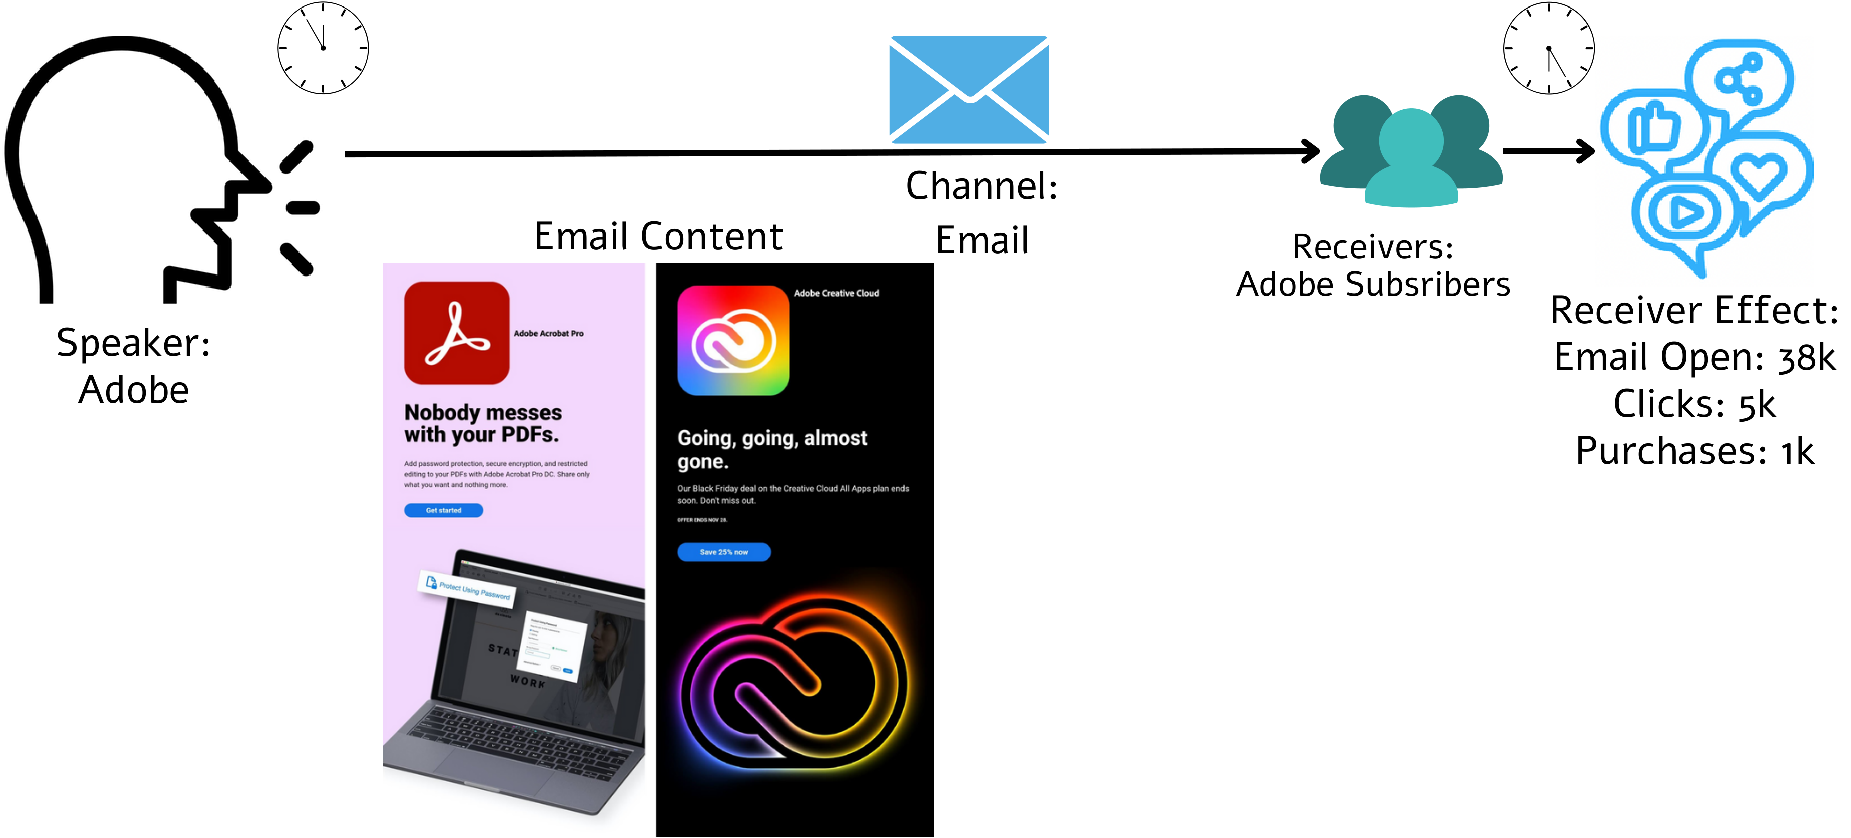
\includegraphics[width=1.0\textwidth]{images/factors of communication.pdf}
  \caption{Communication process can be defined by seven factors: Communicator, Message, Time of message, Channel, Receiver, Time of effect, and Effect. Any message is created to serve an end goal. For marketers, the end goal is to bring in the desired receiver effect (behavior) (like clicks, purchases, likes, and customer retention). The figure presents the key elements in the communication pipeline - the marketer, message, channel, receivers, and finally, the receiver effect.   \label{fig:factors-of-communication}}
\end{figure*}

Historically, behavioral social scientists have sought explanations of human behavior that can provide interpretable causal mechanisms behind human functioning. A few prominent examples are Milgram's \cite{milgram1978obedience} and Asch's \cite{asch1948doctrine} experiments on persuasion, explaining the causal mechanism of obedience to authority. The approach of theorizing has worked in physical sciences where the data is plentiful, and theories make unambiguous predictions but have not been too successful in \textit{predicting} social outcomes in behavioral sciences \cite{open2015estimating,tetlock2017expert,forecasting2023insights}. In fact, many studies have shown that expert human opinions fare similar to non-experts (\textit{e.g.}, predicting economic and political trends \cite{tetlock2017expert}, societal change: \cite{forecasting2023insights}, and advertising success: \cite{singh2024measuring}), and the opinion of non-expert population is roughly the same as a random coin toss in predicting behavior (\textit{e.g.}, predicting cascades \cite{tan2014effect} or image memorability \cite{isola2013makes}). At the same time, causal mechanisms have their own merits; most notably, they help decision-makers (often humans) to make intuitive sense of the situation and make their next decision based on it. 


In parallel, due to the availability of human behavior data at scale, researchers in machine learning are showing a growing interest in traditionally behavioral science topics, such as messaging strategies leading to persuasion \cite{habernal2016makes,kumar2023persuasion,luu2019measuring,bhattacharya2023video}, information diffusion \cite{cheng2014can,martin2016exploring}, and most importantly, prediction and predictability of human behavior \cite{choi2012predicting,song2010limits}. Machine learning approaches bring with them the culture of (training and) testing their models on large real-world datasets and pushing the state-of-the-art in terms of predictive accuracies; at the same time, often, ML approaches can only be operated as black boxes with no direct mechanism to explain predictions \cite{salganik2019bit,singla2022audio}.


In the prediction community, different subfields have emerged dealing with the different parts of the problem of optimization of human behavior. For instance, advertisement personalization studies how to optimize (choose) \textit{receiver} for a given message \cite{chandra2022personalization}, and recommendation systems study how to \textit{choose content} from a set of pre-decided contents for a given receiver to elicit a certain effect \cite{herlocker2004evaluating}. A popular problem within the prediction community is the effect prediction problems, for example, clickthrough (CTR) prediction \cite{mcmahan2013ad}, Twitter cascade prediction \cite{cheng2014can,martin2016exploring}, sales prediction \cite{choi2012predicting,pryzant2017predicting}, content memorability prediction \cite{isola2011makes,khosla2015understanding,si2023long}, \textit{etc}. There are also works to optimize the time of the message to elicit certain effect \cite{newstead2010cost,si2023long}. Some of the major problems studied in behavioral sciences are given below. Through this list, one can observe that all the factors of communication are studied independently in their own light without relying on the underlying unity and continuity of the communication process. 


\begin{enumerate}
\item \textbf{Problems related to optimization in the sender space}:
    \begin{enumerate}
        \item \textbf{Source Optimization}: \textit{Who} should send a particular message over a channel to a specific audience to get the desired behavior? This includes selecting between different brand voices, influencers, spokespersons, or organizational entities based on authority, trustworthiness, and audience affinity.
    \end{enumerate}
    

\item Problems related to Receiver optimization:
    \begin{enumerate}
        \item \textbf{Personalization}: Identifying the optimal receiver for a specific content-channel-time combination to maximize engagement and conversion probability.
        \item \textbf{Customer Segmentation}: Strategic division of the customer base into distinct, actionable groups based on shared characteristics, behaviors, or value propositions to enable differentiated marketing approaches.
        \item \textbf{Social Network Analysis}: Modelling the interconnectedness of receivers (and senders) together in a graph to describe social phenomena like contagion and homophily.
        \item \textbf{Lookalike Modeling}:  Identifying and targeting prospective customers who share similar characteristics, behaviors, and propensities with existing high-value customers or target audiences.
        \item \textbf{Market surveys}: Systematic collection and analysis of primary data about target markets, customer preferences, and competitive landscape to inform marketing decisions.
        \item \textbf{Identity stitching}: Probabilistic and deterministic matching of cross-channel, cross-device customer actions to create unified customer profiles and journey maps.
        \item \textbf{Behavior Explanation}: Discovering causal mechanisms behind a receiver action.
    \end{enumerate}
    
\item \textbf{Problems related to optimization in the content space}:
    \begin{enumerate}
        \item \textbf{Recommender Systems}: Identifying the optimal content that should be delivered next to a certain receiver given a fixed channel, time, and a repository of contents (and their corresponding senders).
        \item \textbf{A/B Testing}: A randomized experiment involving two or more variants with the goal of discovering which variant of a message performs better with a certain audience.
        \item \textbf{Customer Targeting}: Determining what message should be delivered to a target audience segment, targeted based on multi-dimensional attributes (geographic, demographic, behavioral, and psychographic) through particular channels.

        \item \textbf{Propensity Modelling or Engagement Modelling}: Modeling probability of engagement in terms of actions like Clickthrough, social media actions such as likes and shares for a certain audience, sender, and campaign.
        \item \textbf{Transsuasion}: Conversion of a content from low-performing to high-performing for a given audience, sender, and time, while maintaining the content's intent, style, and emotional impact.
        \item \textbf{Transcreation}: Conversion of a content designed for one audience (like a particular culture) to another audience, while maintaining the content's intent, style, and emotional impact.
        \item \textbf{Search Engine Optimization}: Improving the quality and quantity of website traffic to a website from search engines by doing content optimization (like adding keywords, backlinks, \textit{etc}).
        \item \textbf{Performant Content Generation}: Generate content that can perform better for a given audience, sender, time, and goal.
        \item \textbf{Argument Mining}: Automatic extraction and identification of argumentative structures from natural language text.
        \item \textbf{Persuasion Strategies}: Use of rhetorical devices (such as emotion, social identity, and scarcity) to optimize the effect of a message on a certain audience.
    \end{enumerate}

\item \textbf{Problems related to optimization in the channel space}:
    \begin{enumerate}
        \item \textbf{Channel Optimization}: Optimizing channels for a particular audience, sender, time, and goal.
        \item \textbf{Marketing Mix Modeling}: Measuring and attributing the impact of various decisions like channel investments, discounts, promotional campaigns in their contribution to engagement and sales. 
        \item \textbf{Auction Design} and \textbf{Bidding}: Mechanisms to discover the cost of attention of a certain receiver to a particular sender, time, and campaign goal.
    \end{enumerate}
    
\item \textbf{Problem related to optimization in the time space}:
    \begin{enumerate}
        \item \textbf{Send Time Optimization}: Determining the optimal timing for message delivery for a certain receiver, sender, content combination.

        \item \textbf{Trend Forecasting}: Projecting marketing and social trends in the future.
    \end{enumerate}
        
\end{enumerate}







A common theme that runs through both research cultures in behavioral sciences is the intent to control behavior. Explanation and prediction are intermediate steps to control and hence optimize behavior. Optimizing behavior means to fulfill the communicator's objectives by controlling the other six parts of the communication process (Fig.~\ref{fig:factors-of-communication}). Due to the problem space being large, the solution needs a general understanding of human behavior as opposed to being domain-specific. In this thesis, our aim is to make such models that can develop this general understanding.


The characteristic that marks the digital age is the prevalence of human behavioral data in huge repositories. This data is \textit{big} (allowing to model heterogeneity), \textit{always-on} (allowing to look in the past as well as live measurements), observational (as opposed to reactive), but also \textit{incomplete} (does not capture all that is happening everywhere everytime in a single repository) and \textit{algorithmically confounded} (generated as a byproduct of an engineering process with a goal) \cite{salganik2019bit}. While the predictive culture has tried to make use of some of this data in the form of social media datasets like Twitter \cite{tumasjan2010predicting,asur2010predicting} and Instagram \cite{kim2020multimodal}, Google trends \cite{choi2012predicting,carriere2013nowcasting}, Wikipedia \cite{generous2014global,de2021general,mestyan2013early}, shopping websites \cite{krumme2013predictability,de2015unique} and other data sources \cite{brockmann2006scaling,song2010limits,miritello2013limited}, these efforts are limited, in the sense of being dependent on one or a few chosen platforms, able to answer a limited set of questions, and restricted by access to private data. We want a model that can understand (predict and explain) \textit{human behavior in general} as opposed to modeling a particular effect (retweet prediction) on a particular platform (\textit{e.g.} Twitter) for a certain type of users.
This problem carries parallels with the problem being solved in the natural language processing (NLP) community, where supervised models in NLP are limited by the amount of supervision available and being able to answer one question (for which the supervised model was trained). The problem was solved by developing Large Language Models (LLMs), which are general purpose models capable of \textit{understanding language}, and hence can solve natural language tasks like sentiment analysis, question answering, email generation, and language translation in zero-shot (\textit{i.e.} without needing any explicit training for that task) \cite{devlin2018bert,brown2020language,radford2018improving,raffel2020exploring,radford2019language}.




\begin{figure*}[h]
  \centering
  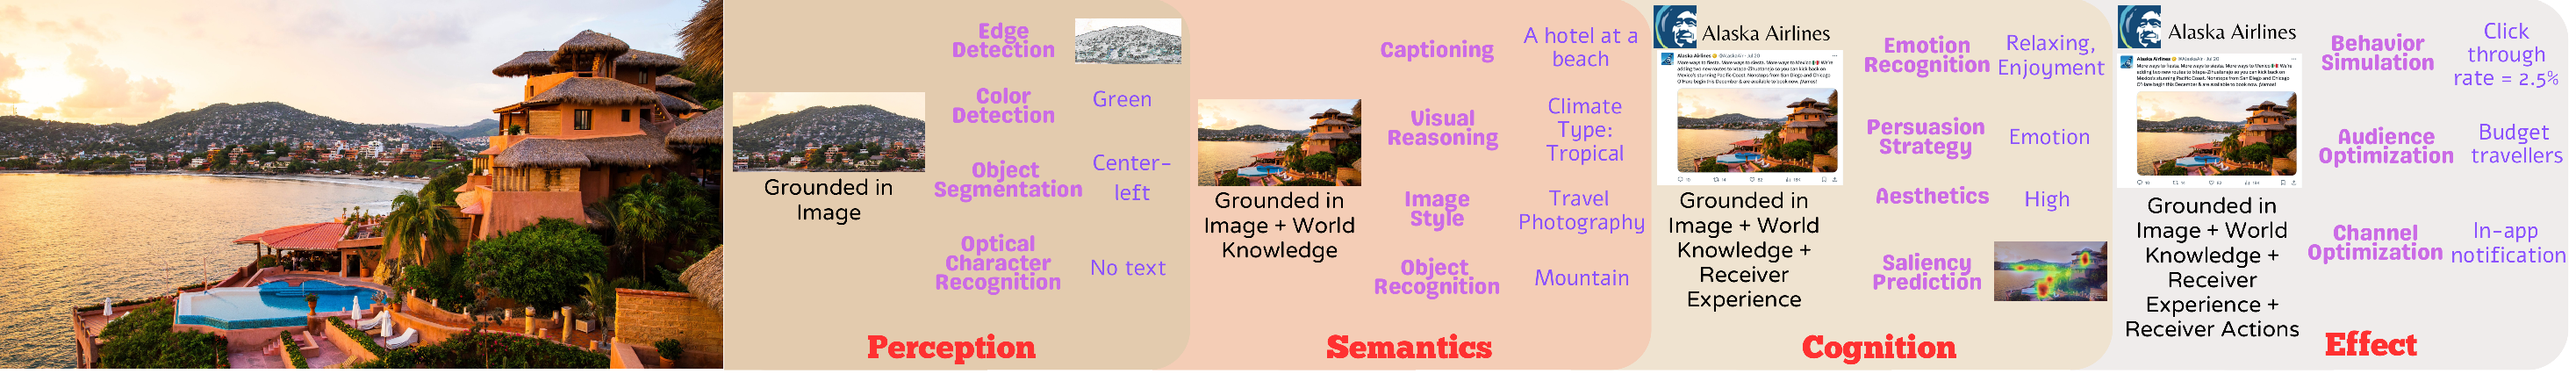
\includegraphics[width=1.0\textwidth]{images/levels of analysis.pdf}
  \caption{Levels of content analysis. The figure lists tasks and their sample outputs arranged in a hierarchy \cite{shannon-weaver-1949}. This is roughly based on levels of language. Notably, humans are good at predicting the first three levels but not the last level \cite{tetlock2017expert,forecasting2023insights,tan2014effect,isola2013makes}. 
  \label{fig:levels of content analysis}
  }
\end{figure*}



Similarly, how do we develop a model capable of understanding behavior \textit{in general}? With the intent to answer this question, we take motivation from LLMs, where the idea is to train a model on a data-rich task. The task chosen to train LLMs is the next-word prediction, and the dataset is the text collected from the entire internet. The next-word prediction task is a data-rich task that can be trained on the huge text repositories from the internet. The intuition is that two approaches have always worked for neural networks: larger model sizes and more data for training \cite{mikolov2013efficient,devlin2018bert,radford2018improving,raffel2020exploring}. Going from a few million tokens of text \cite{mikolov2013efficient,radford2018improving} to a trillion tokens \cite{touvron2023llama,brown2020language} leads to an increase in the transfer learning capability leading to performance improvements over a wide variety of natural language tasks. 


The digital revolution has provided us with huge repositories of data. We leverage the human behavior repositories available on the internet for this general-purpose human behavior model. The format of this data is the general communication model shown in Fig.~\ref{fig:factors-of-communication} consisting of communicator, message, time of message, channel, receiver, time of effect, and effect. Due to the incomplete nature of behavioral repositories, all the factors are usually not always available. However, a subset is always available, and we show that the data scale, along with a large model, helps make a general behavior understanding model \cite{khandelwal2023large}. We call this model, Large Content and Behavior Model (LCBM). We show that LCBM can predict behavior, explain it, and generate a message to bring about certain behavior \cite{si2023long,khandelwal2023large,khurana2023behavior}. 



\textit{Are general LLMs unable to solve behavioral problems?} A question that arises is whether LLMs, which already learn trillions of text tokens, are able to understand and predict behavior. We investigate that question over several large models, including GPT-3.5 \cite{brown2020language}, GPT-4 \cite{openai2023gpt4}, Llama-13 B and LLama-7B \cite{touvron2023llama}, and find that they are unable to solve the behavioral problems listed before. The reason for this is that large language models only include one factor (message) out of the 7-factor communication model (Fig.~\ref{fig:factors-of-communication}) while considering other parts as ``noise'' (for instance, see \cite{biderman2022datasheet,penedo2023refinedweb}). This systematic purge of communicator, receiver, channel, time, and, most importantly, behavior causes the models not to develop any behavioral capabilities (Level-C of Shannon and Weaver \cite{shannon-weaver-1949}). As an example, Llava \cite{liu2023visual}, a recent large language and vision model (VLM) trained by connecting a vision encoder with a language model, shows that after training on a few hundred thousand instructions, the language model can now ``see'', and is able to answer questions on the images. However, the questions all lie in the first two levels of content analysis shown in Fig.~\ref{fig:levels of content analysis}. The reason is that the instructions used to align the image encoder with the downstream LLM all lie in the first two levels (sender and message) while ignoring the last two (receiver and behavior). In the upcoming chapters, we explore how we can train a general behavior model and how including the other factors of communication back in training data helps in understanding human behavior.


%Notably, this is the forward path of communication in which, as time progresses, a message originates, travels in a channel, is received by the subscribers, and finally generates an effect. 
%Effect (or behavior) over a content can also enable us to understand about the content, the communicator, the receiver, or the time. Therefore, efforts have also been made to extract information about the content itself from the behavior it generates. 



% XXX: to be improved In social science and computational social science cultures, research is carried out to discover causal effects and model them. For instance, propaganda and mass communication studies \cite{mcquail1987mass,krippendorff2018content,lasswell1948structure,lasswell1971propaganda} try to understand the culture, time, authors, recipients in a non-invasive manner using the messages exchanged, and persuasion studies \cite{petty1981effects,chaiken1980heuristic} where the persuasion strategy present in the content is identified and correlated with (un)successful efforts of persuasion. 



\begin{figure*}[!t]
  \centering
  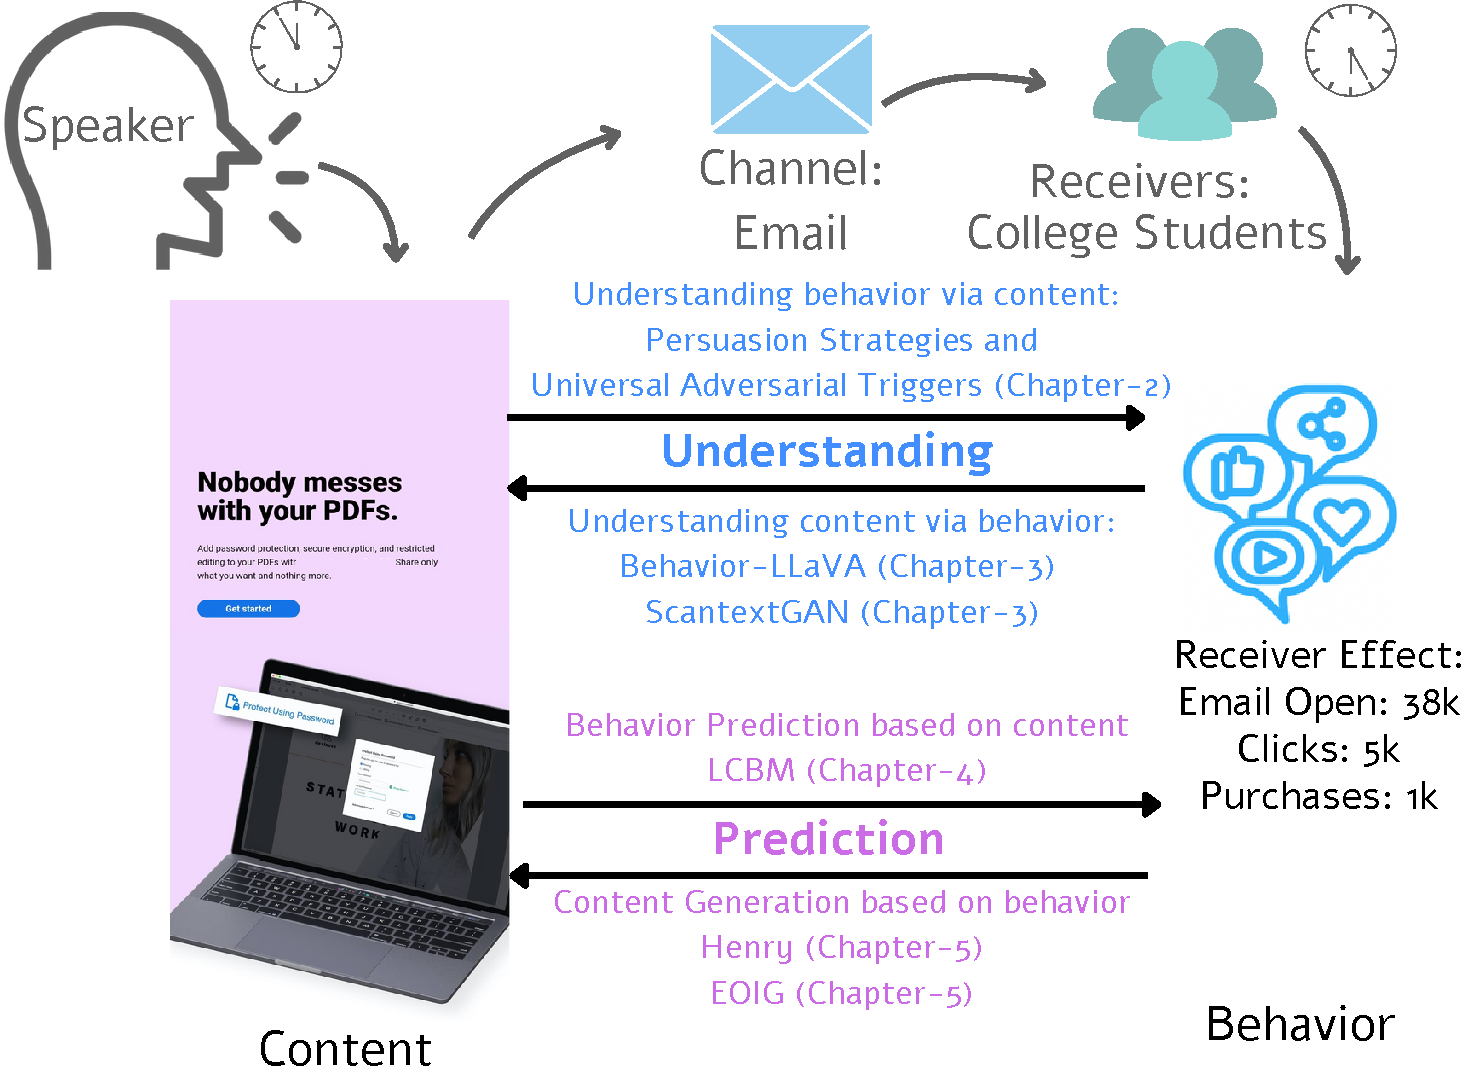
\includegraphics[width=0.7\textwidth]{images/thesis-link.pdf}
  \caption{Communication process can be defined by seven factors: Communicator, Message, Time of message, Channel, Receiver, Time of effect, and Effect. Any message is created to serve an end goal. In this thesis, we explore the two main concerns of behavioral sciences: understanding (or explanation) and prediction. The figure shows the links between the different chapters and how they link together to form the two core pillars of understanding and explanation. \label{fig:factors-of-communication-thesis-links}}
\end{figure*}



\textit{Outline for the upcoming chapters}: Following the two traditions of behavioral sciences, we delve into both explanation and prediction. Figure~\ref{fig:factors-of-communication-thesis-links} gives a visual description of the various chapters and how they link with each other. In Chapter-\ref{chatper:Explaining Behavior: Persuasion Strategies}, we start with a more traditional approach to behavior explanation, where we cover the first works on extracting persuasion strategies in advertisements (both images and videos) \cite{kumar2023persuasion,bhattacharya2023video}. The contributions of these works include constructing the largest set of generic persuasion strategies based on theoretical and empirical studies in marketing, social psychology, and machine learning literature and releasing the first datasets to enable the study and model development for the same. These works have been deployed to understand the correlation between the kinds of marketing campaigns and customer behavior measured by clicks, views, and other marketing key performance indicators (KPIs). Further, we also introduce methods called universal adversarial triggers (UATs) to mine behavioral models to understand what they learn. This approach provides a converse approach for human behavior understanding. While persuasion strategies help a human correlate and understand content (message) and behavior, universal adversarial triggers help understand what models learn, which makes them successful in predicting behavior.



Following this, in Chapter-\ref{chatper:Content and Behavior Models}, we delve into the question of modeling behavior. The key insight behind this chapter is that behavior is always produced by a receiver in response to a content sent by a sender at a time. We model behavior together with the pieces of sender, receiver, time, and content. We show that while large language models already model content, they do not model the other pieces of sender, receiver, and time. We model these factors together and show emergent abilities in understanding behavior. We observe that teaching the Large Content and Behavior Models (LCBM) behavior and content simulation improves its capabilities on them (expected), but the model also shows signs of domain-adaptation in behavior modality (few-shot capability, unexpected) and improvements in behavior understanding (zero-shot capability, unexpected). To spur research on the topic of large content and behavior models, we release our generated behavior instruction fine-tuning data from over 40,000 public domain YouTube videos and 168 million Twitter posts. The data contains: 1) YouTube video links, automatically extracted key scenes, scene verbalizations, replay graph data, video views, likes, comments, channel name, and subscriber count at the time of collection, and 2) Twitter extracted account names, tweet text, associated media (image and video) verbalizations (including image captions, keywords, colors, and tones), tweet timestamps, and like counts. We also release a benchmark to test performance on the joint content behavior space introducing two types of tasks in this space: predictive and descriptive. In the predictive benchmark, we test the model’s ability to predict behavior given the content and predict content given the behavior. In the descriptive benchmark, we validate its explanation of human behavior by comparing it with ground-truth annotations we obtain from human annotators that try to explain human behavior.



Next, in Chapter~\ref{chapter:Encoding Behavior To Improve Content Understanding}, we analyze the communication process in more detail. As behavior is the signal a receiver emits when a sender sends a content; similarly, one can see this behavior emitted as a content in the next cycle, where the receiver becomes the sender, and the sender becomes the receiver. Therefore, we ask if we can understand the content better by modeling behavior. For example, a person's heightened state of emotional response, like dilated pupils and sweat, while watching an action scene from the movie Jurassic Park gives us much information about the scene itself. Today's models are built only on content (the Jurassic Park movie itself) while ignoring the human behavioral responses over the content. Behavioral responses like likes, shares, comments, replay graphs, and upvotes are freely available and waiting to be integrated into the workflow to understand content better. We show evidence for this hypothesis by improving LLMs across 46 different tasks over 23 benchmark datasets across all four modalities of language, audio, text, and video. The hypothesis of extracting and using signals from behavior is lately getting attention in the fields of human alignment and reinforcement learning with human feedback (RLHF) where researchers try to use human behavioral signals of likes, upvotes, and annotations of a response's helpfulness to improve content generation \cite{kreutzer2018can,stiennon2020learning,ziegler2019fine,nakano2021webgpt,si2023long,lee2023aligning,wu2023better,khurana2023behavior,khurana-etal-2023-synthesizing}. In our work, we propose a scalable approach to increase the content understanding abilities of VLMs, requiring minimal cost and no architectural changes. 

%the more modern approach of behavior prediction and leveraging the huge repositories of behavior data available. First, we propose models to integrate behavior with relatively smaller language models like BERT \cite{devlin2018bert}, and show that the resultant models can understand content better than the base models \cite{khurana-etal-2023-synthesizing}. Then, we propose an approach to integrate behavior and content together as part of a single model. We call these models Large Content and Behavior Models (LCBM) \cite{khandelwal2023large}. We show that these models can predict and explain behavior. 

%Diagram for chapters 



Communication serves as a fundamental mechanism for achieving shared goals between senders and receivers \cite{smith2003animal}. Humans possess a remarkable capacity to cooperate with strangers, enabled by language that has allowed our ancestors to exchange information, resolve conflicts, and create shared constructs like fictions, social structures, and cultural frameworks \cite{misyak2016instantaneous,mccroskey2015introduction,smith1997major}. This ability emerges early in human development, with children demonstrating communication and persuasion skills from a young age \cite{perner1985john}. Notably, strategic communication extends beyond human species, manifesting in both conspecific \cite{hare2000chimpanzees,smith2003animal} and interspecific \cite{krebs1984animal,fouts200235} interactions. A compelling example is the "broken wing display" observed across various bird genera, where adults feign injury to appear vulnerable, strategically luring predators away from their offspring \cite{griffin2001animal}.
Building on this foundation of strategic communication, the final chapter of this thesis (Chapter-\ref{chatper:Generating Content Leading to Optimal Behavior}) demonstrates how modeling the complete communication workflow enables the generation of messages designed to elicit specific behavioral outcomes. We explore this concept across two modalities:

\begin{enumerate}
    \item Text Domain: Through the illustrative case of memorability, we develop methods to generate content that demonstrates enhanced long-term retention \cite{si2023long}.

    \item Visual Domain: We advance techniques for generating images that achieve higher performance metrics, specifically focusing on engagement through social media likes \cite{khurana2023behavior}.

\end{enumerate}


In addressing these challenges, we make several key contributions:
First, we introduce UltraLAMBDA, the first large-scale advertisement dataset, comprising 5 million ads with automatically extracted content labels, including ASR transcriptions, captions, OCR text, emotion indicators, and memorability scores assigned by our model. Our analysis reveals that current large language models (LLMs) like GPT-3.5 and GPT-4 struggle to generate inherently memorable content. In response, we developed Henry, which demonstrates a 44\% average improvement in memorability scores through progressive generation techniques. This work represents the first successful application of synthetic data to a domain previously lacking large-scale training resources.


Second, we address the critical need for engagement-optimized image generation, particularly relevant to industries such as advertising, fashion, and e-commerce, where user engagement metrics (clicks, likes, purchases) directly measure success. We present EngagingImageNet, a comprehensive dataset containing 168 million tweets collected from 10,135 enterprise accounts (2007-2023). This dataset includes rich metadata: account information, tweet text, media content, image captions, keywords, color analysis, posting timestamps, and engagement metrics. 

Our analysis reveals that traditional image generation metrics (fidelity, aesthetics) show no correlation with actual engagement. To bridge this gap, we developed EngageNet, an engagement-aware vision language model (VLM) capable of predicting user engagement levels for images. Building on EngageNet's capabilities, we release Engagement Arena, the first automated benchmark for assessing the engagement potential of text-to-image models. This platform not only enables systematic comparison of existing models but also provides an open framework for the research community to evaluate and improve engagement-oriented image generation techniques.







%We release the first large scale ad dataset, UltraLAMBDA, consisting of 5 million ads with their automatically extracted content labels like ASR, captions, OCR, emotions, and memorability scores assigned by Henry. Using Ultra-LAMBDA, we first show that large LLMs like GPT-3.5 and 4 are unable to generate memorable content. Then, we train Henry to progressively generate more memorable ads resulting an average improvement of 44\% in memorability scores. Through this, for the first time in literature, we also show the use of synthetic data on a task for which no large scale data exists.


%Images, especially in industries like advertising, fashion, and e-commerce, are created to achieve user engagement in the form of clicks, likes, and purchases. Therefore, the image generation process needs to be biased on the image’s eventual utility, in addition to the common goals of high aesthetics and fidelity. We curate EngagingImageNet, a large-scale, high-quality dataset consisting of user engagement over images. EngagingImageNet consists of 168 million tweets collected from 10,135 enterprise Twitter accounts from the time period 2007 to 2023. It consists of the account name, tweet text, media posted with the tweet, image captions, keywords, colors and tones, the time of posting, and the number of likes the image received. The dataset is instrumental in our study of image engagement as the utility in real-world marketing scenarios. We show that existing image generation metrics like fidelity, aesthetic scores and such are not correlated with engagement. Therefore, we train an engagement-aware vision language model (VLM), called EngageNet, to predict user engagement over images. EngageNet exhibits strong performance in estimating user engagement. Using EngageNet’s predicted engagement scores as a reward, we introduce Engagement Arena, the first automated arena to benchmark the engagement of text-to-image models. We rank several popular text-to-image models on their ability to generate engaging images and further encourage the community to submit their models to the arena. We demonstrate introducing the goal of engagement in the text-to-image generation process. 



Therefore, we will cover explanation, analysis, prediction, and generation aspects of behavior. We will cover the following works in this thesis:
\begin{enumerate}
    \item MINIMAL: Mining models for data-free universal adversarial triggers. AAAI, 2022, (covered in Chapter-\ref{chatper:Explaining Behavior: Persuasion Strategies})

    \item Persuasion Strategies in Advertisements, AAAI, 2023, (covered in Chapter-\ref{chatper:Explaining Behavior: Persuasion Strategies})

    \item A Video Is Worth 4096 Tokens: Verbalize Videos To Understand Them In Zero Shot, EMNLP, 2023, \textbf{Nominated for best paper award} (covered in Chapter-\ref{chatper:Explaining Behavior: Persuasion Strategies})

    \item Large Content And Behavior Models To Understand, Simulate, And Optimize Content And Behavior, ICLR, 2024, \textbf{Nominated for best paper award} (covered in Chapter-\ref{chatper:Content and Behavior Models})
    
    \item Synthesizing Human Gaze Feedback for Improved NLP Performance, EACL, 2023 (covered in Chapter-\ref{chapter:Encoding Behavior To Improve Content Understanding})

    \item Teaching Human Behavior Improves Content Understanding Abilities Of VLMs, Arxiv preprint (under review), 2024 (covered in Chapter-\ref{chapter:Encoding Behavior To Improve Content Understanding})

    \item Long-Term Ad Memorability: Understanding and Generating Memorable Ads, WACV, 2025 (covered in Chapter-\ref{chatper:Generating Content Leading to Optimal Behavior})

    \item Measuring And Improving Engagement of Text-to-Image Generation Models, Arxiv preprint (under review), 2024 (covered in Chapter-\ref{chatper:Generating Content Leading to Optimal Behavior})
\end{enumerate}



\begin{comment}
    They mentioned that the broad problem of communication can be studied at three levels: technical, semantic, and effectiveness. 
    \textbf{Level A: Technical.} How accurately can the symbols of communication be transmitted?
    
    \textbf{Level B: Semantic.} How precisely do the transmitted symbols convey the desired meaning?
    
    \textbf{Level C: Effectiveness.} How well does the received meaning induce the desired conduct in the receiver?
    
    These three levels build on top of each other. Thus, solving the problem at Level C necessarily requires solving the corresponding problems at Levels A and B.
    
    Since the publication of this seminal paper, the tremendous growth in the field of telecommunications, particularly the advent of the Internet and mobile devices, has led to affordable, wide-scale solutions for Level A.
    With the recent advances in large language models (LLMs) such as BERT \citep{devlin2018bert}, GPT-3 and 4 \citep{brown2020language,openai2023gpt4}, T5 \citep{raffel2020exploring}, and many more, we have witnessed a significant improvement in the performance of various Natural Language Processing (NLP) tasks. LLMs in zero- or few-shot settings can easily handle tasks such as question answering, summarization, translation, and many more. This has helped us progress towards solving Level B to a large extent. However, there has been limited progress in Level C, the effectiveness problem. 
    
    
    
    Effectiveness refers to communicating to fulfill the communicator's objectives.
\end{comment}


\chapter{Explaining Behavior: Persuasion Strategies and Universal Adversarial Triggers}
\label{chatper:Explaining Behavior: Persuasion Strategies}


\begin{figure}[t]
    % \vspace{-38mm}
    \centering
    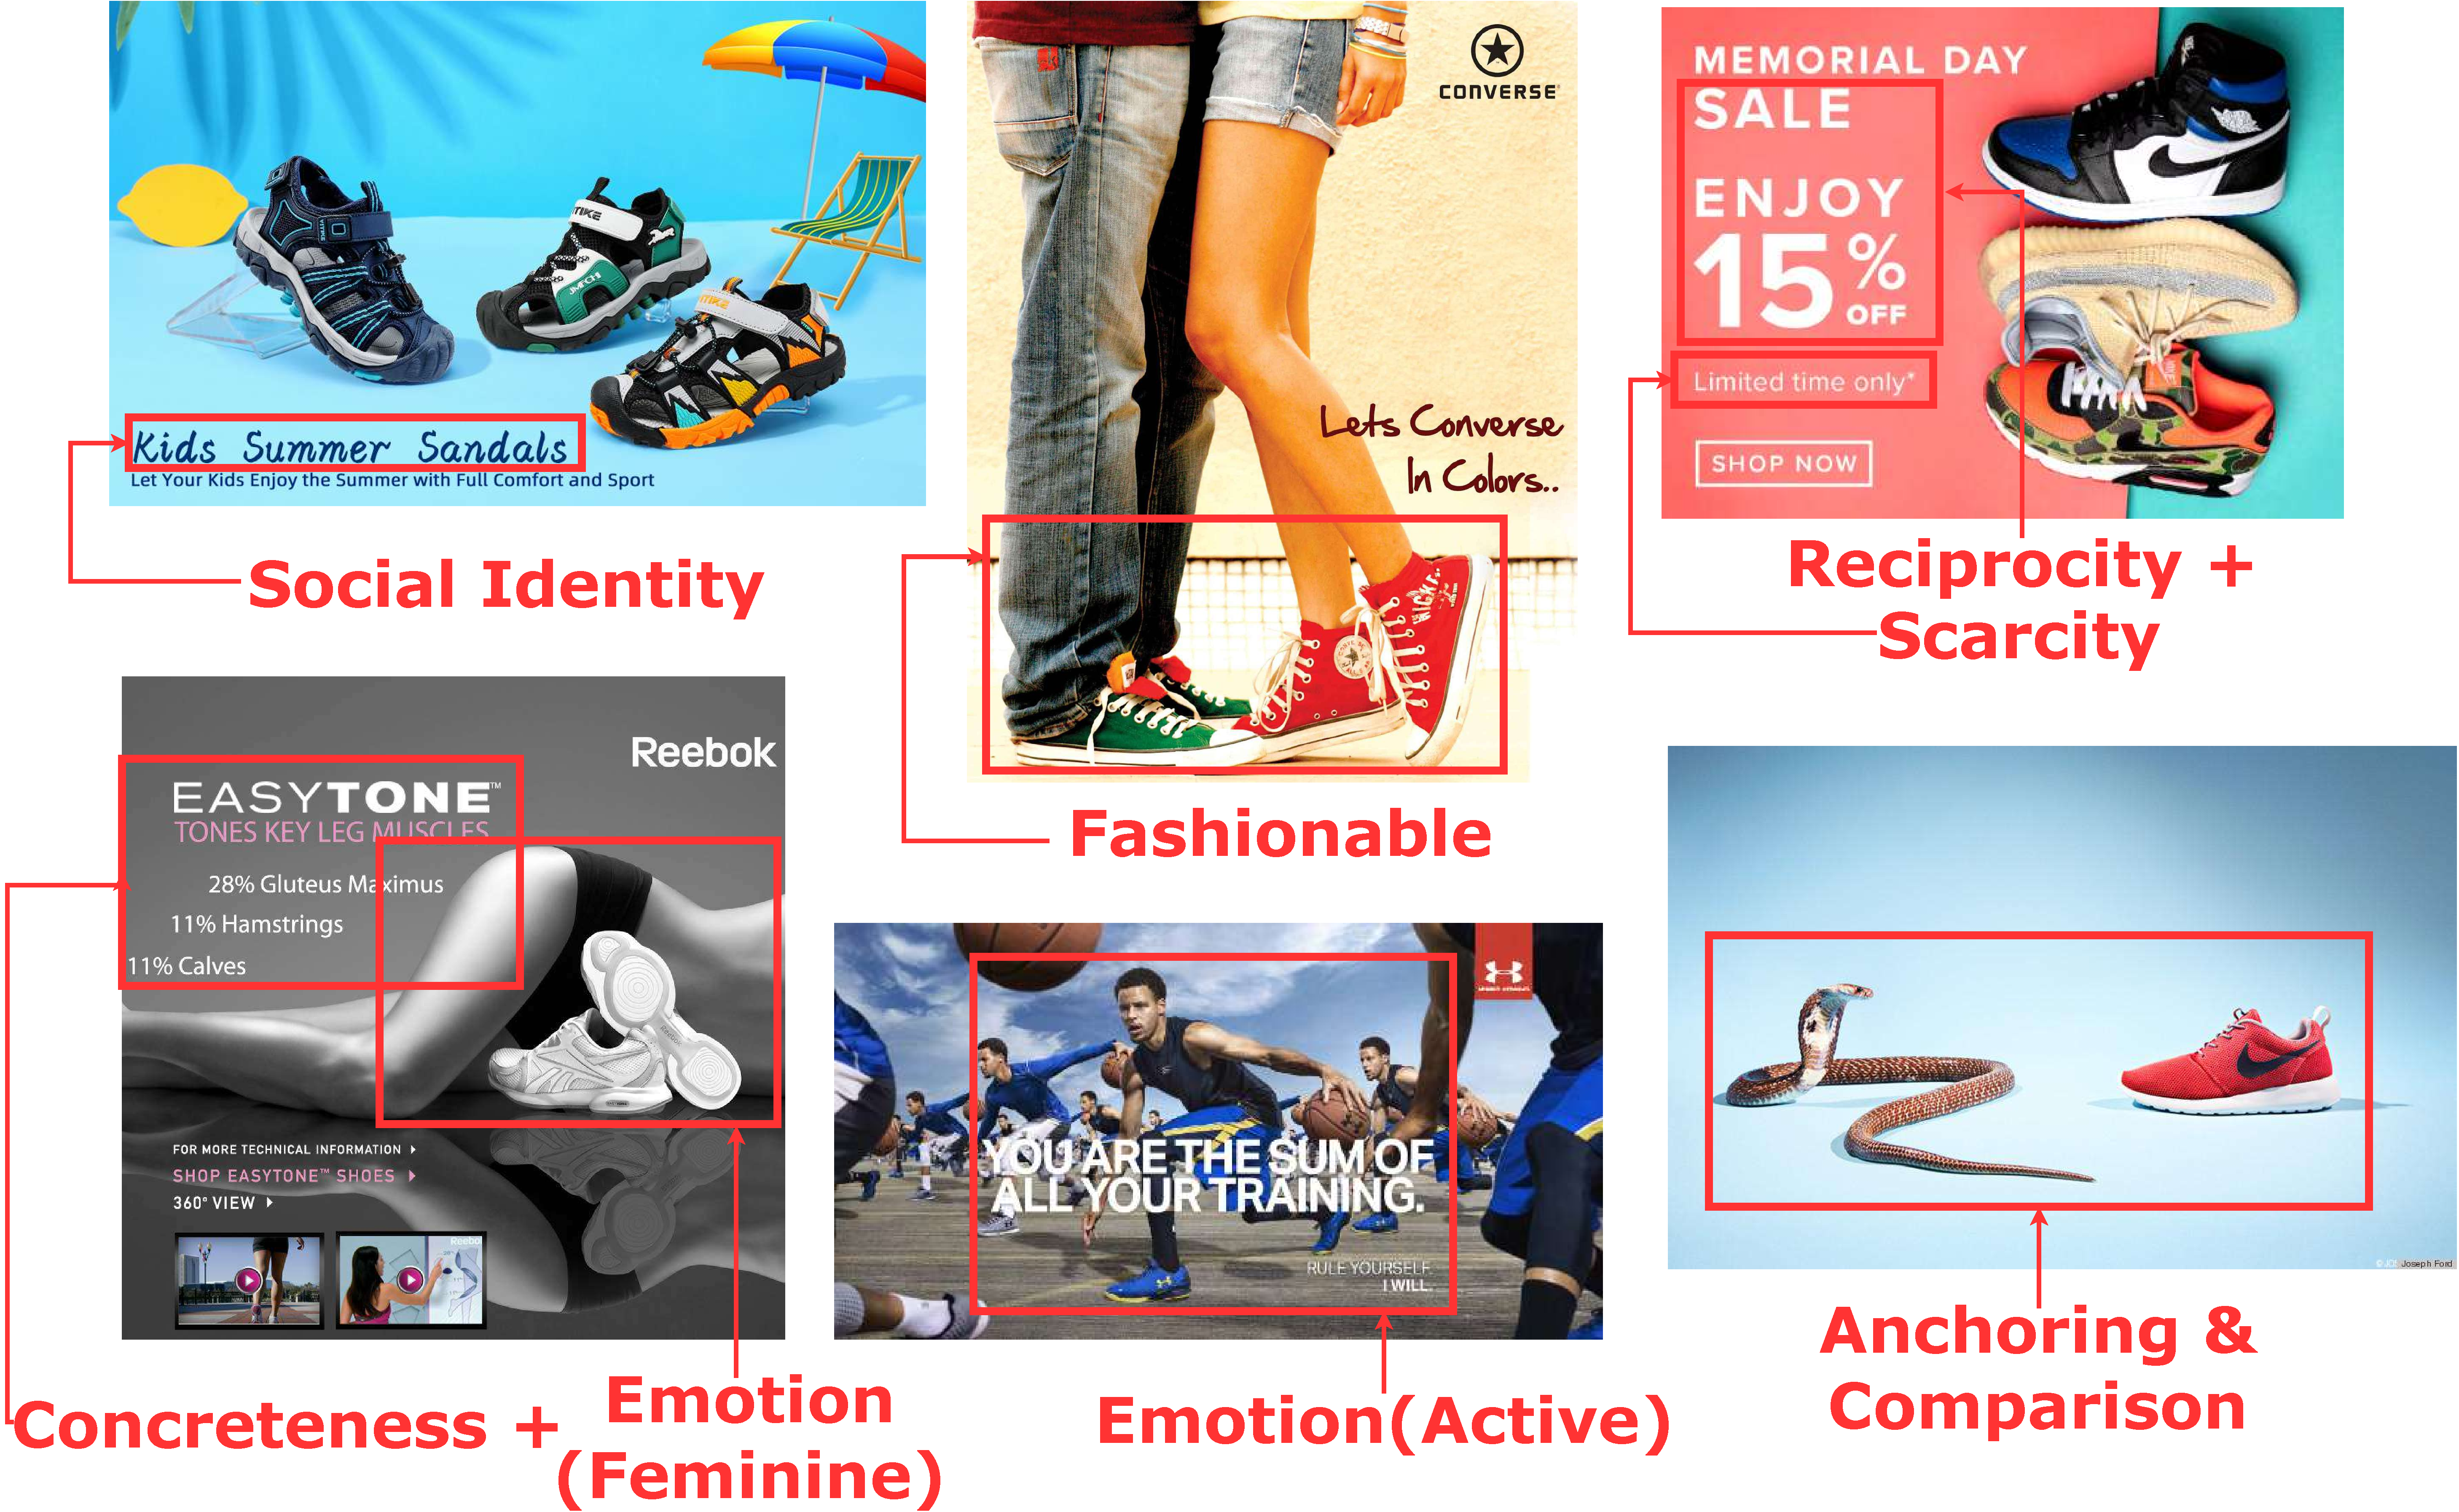
\includegraphics[width=0.8\textwidth]{images/footwear-strategies.pdf}
    \caption{Different persuasion strategies are used for marketing the same product (footwear in this example). The strategies are in red words and to be defined by us in the paper.}
    \label{fig:footwear-strategies}
    % \vspace*{-4mm}
\end{figure}


\begin{figure*}[!ht]
    \centering
    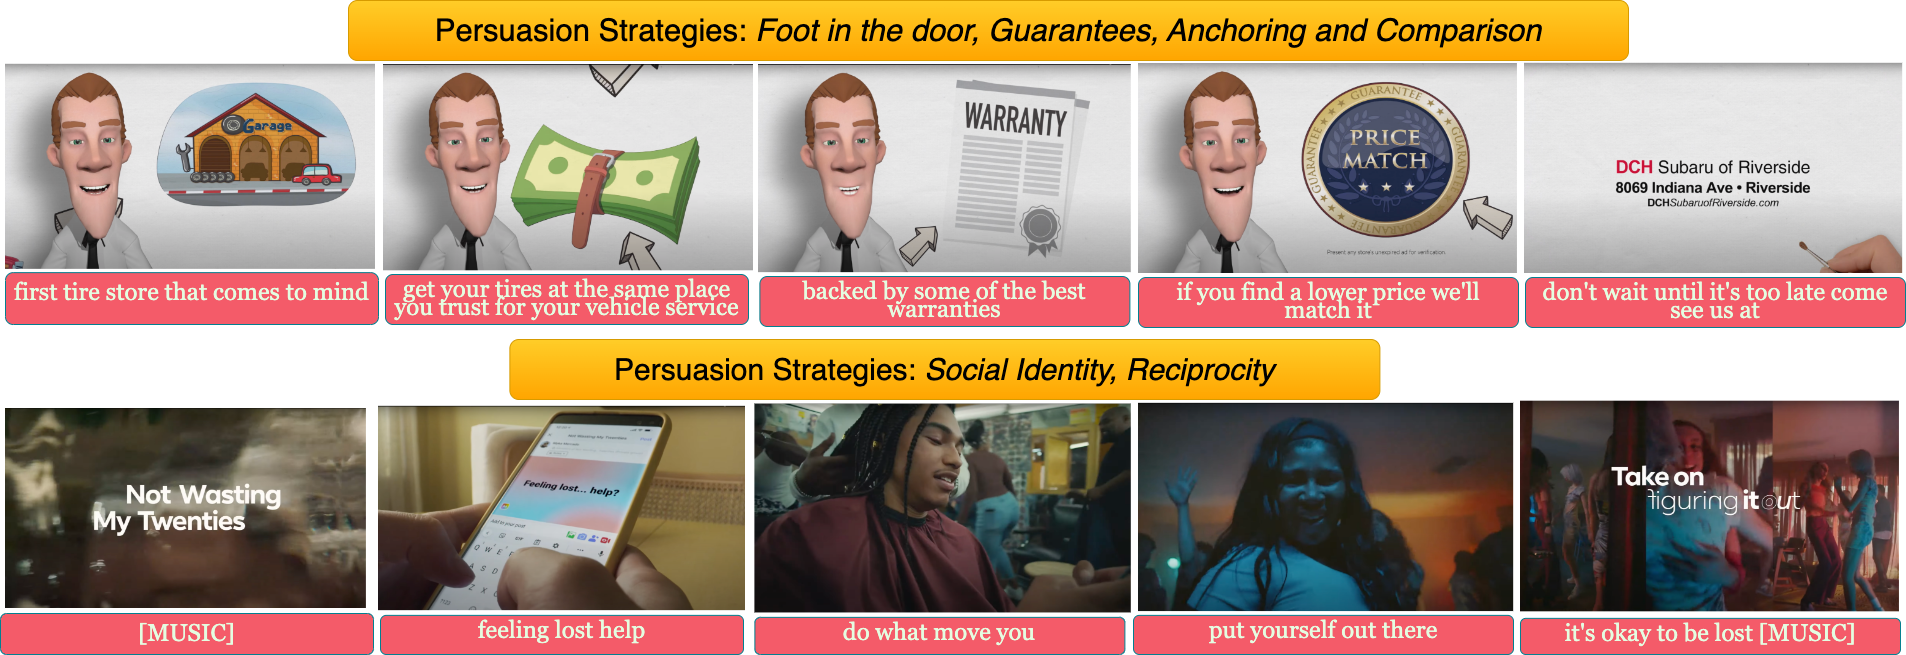
\includegraphics[width=\textwidth]{images/persuasion-strategies-videos.png}
    \caption{Examples of videos with their annotated persuasion strategies. Relevant keyframes and ASR captions are shown in the figure, along with the annotated strategies. These two videos can be watched at 
    \url{https://bit.ly/3Ie3JG0}, \url{https://bit.ly/3OgtLwj}
    .}
    \label{fig:persuasion-strategy-dataset-examples}
\end{figure*}



Modeling what makes an advertisement persuasive, \textit{i.e.}, eliciting the desired response from consumer, is critical to the study of propaganda, social psychology, and marketing. Despite its importance, computational modeling of persuasion in computer vision is still in its infancy, primarily due to the lack of benchmark datasets that can provide persuasion-strategy labels associated with ads. Motivated by persuasion literature in social psychology and marketing, as the first contribution, we introduce an extensive vocabulary of persuasion strategies and build the first ad corpus (both image and video) annotated with persuasion strategies (Section~\ref{sec:chapter-2 Persuasion Strategies In Advertisements}). We then formulate the task of persuasion strategy prediction with multi-modal learning. The image dataset also provides image segmentation masks, which labels persuasion strategies in the corresponding ad images on the test split. We publicly release our code and dataset at \url{https://midas-research.github.io/persuasion-advertisements/}. This section is based on two papers \cite{kumar2023persuasion,bhattacharya2023video}.


Persuasion strategies offer a human-interpretable framework for understanding persuasion and its influence on behavior. Another focus of my work is to uncover what models trained to predict behavior actually learn. Advances in deep learning and large language models have significantly improved the accuracy of behavior prediction \cite{khandelwal2023large}, but they have also increased the models' opacity, making them more like black boxes. Investigating what these \textit{behavior prediction models understand about behavior} can provide insights that may be challenging to derive from first principles. This motivation underpins our other work \cite{singla2022minimal}, discussed in Section~\ref{MINIMAL: Mining models for universal adversarial triggers}. In this work, we mine behavioral prediction models to understand what they learn about behavior which makes them so successful at behavior prediction. This approach is complementary to the approach afforded by persuasion strategies. While persuasion strategies help humans summarize all messages to predict and understand behavior, our method, called universal adversarial triggers (UATs) help us understand a model's global behavior. We observe that content words with the lowest entropy appear as UATs. We explain this idea with the help of several models and datasets.



\section{Persuasion Strategies In Advertisements}
\label{sec:chapter-2 Persuasion Strategies In Advertisements}


Marketing communications is the mode by which companies and governments inform, remind, and persuade their consumers about the products they sell. They are the primary means of connecting brands with consumers through which the consumer can know what the product is about, what it stands for, who makes it, and can be motivated to try it out. To introduce meaning into their communication, marketers use various rhetorical devices in the form of persuasion strategies such as \textbf{emotions} ({\it e.g.}, Oreo's ``Celebrate the Kid Inside'', humor by showing Ronald McDonald sneaking into the competitor Burger King's store to buy a burger), \textbf{reasoning} ({\it e.g.}, ``One glass of Florida orange juice contains 75\% of your daily vitamin C needs''), \textbf{social identity} ({\it e.g.}, Old Spice's ``Smell like a Man''), and \textbf{impact} ({\it e.g.}, Airbnb showing a mother with her child with the headline ``My home is funding her future'') (Refer to Fig.~\ref{fig:rhetoric-strategies-ads} to see these ads). Similarly, even for marketing the same product, marketers use different persuasion strategies to target different demographies (see Fig.~\ref{fig:footwear-strategies}). Therefore, recognizing and understanding persuasion strategies in ad campaigns is vitally important to decipher viral marketing campaigns, propaganda, and enable ad-recommendation. 




\begin{figure*}
    \centering
    \begin{subfigure}[b]{0.4\textwidth}
         \centering
         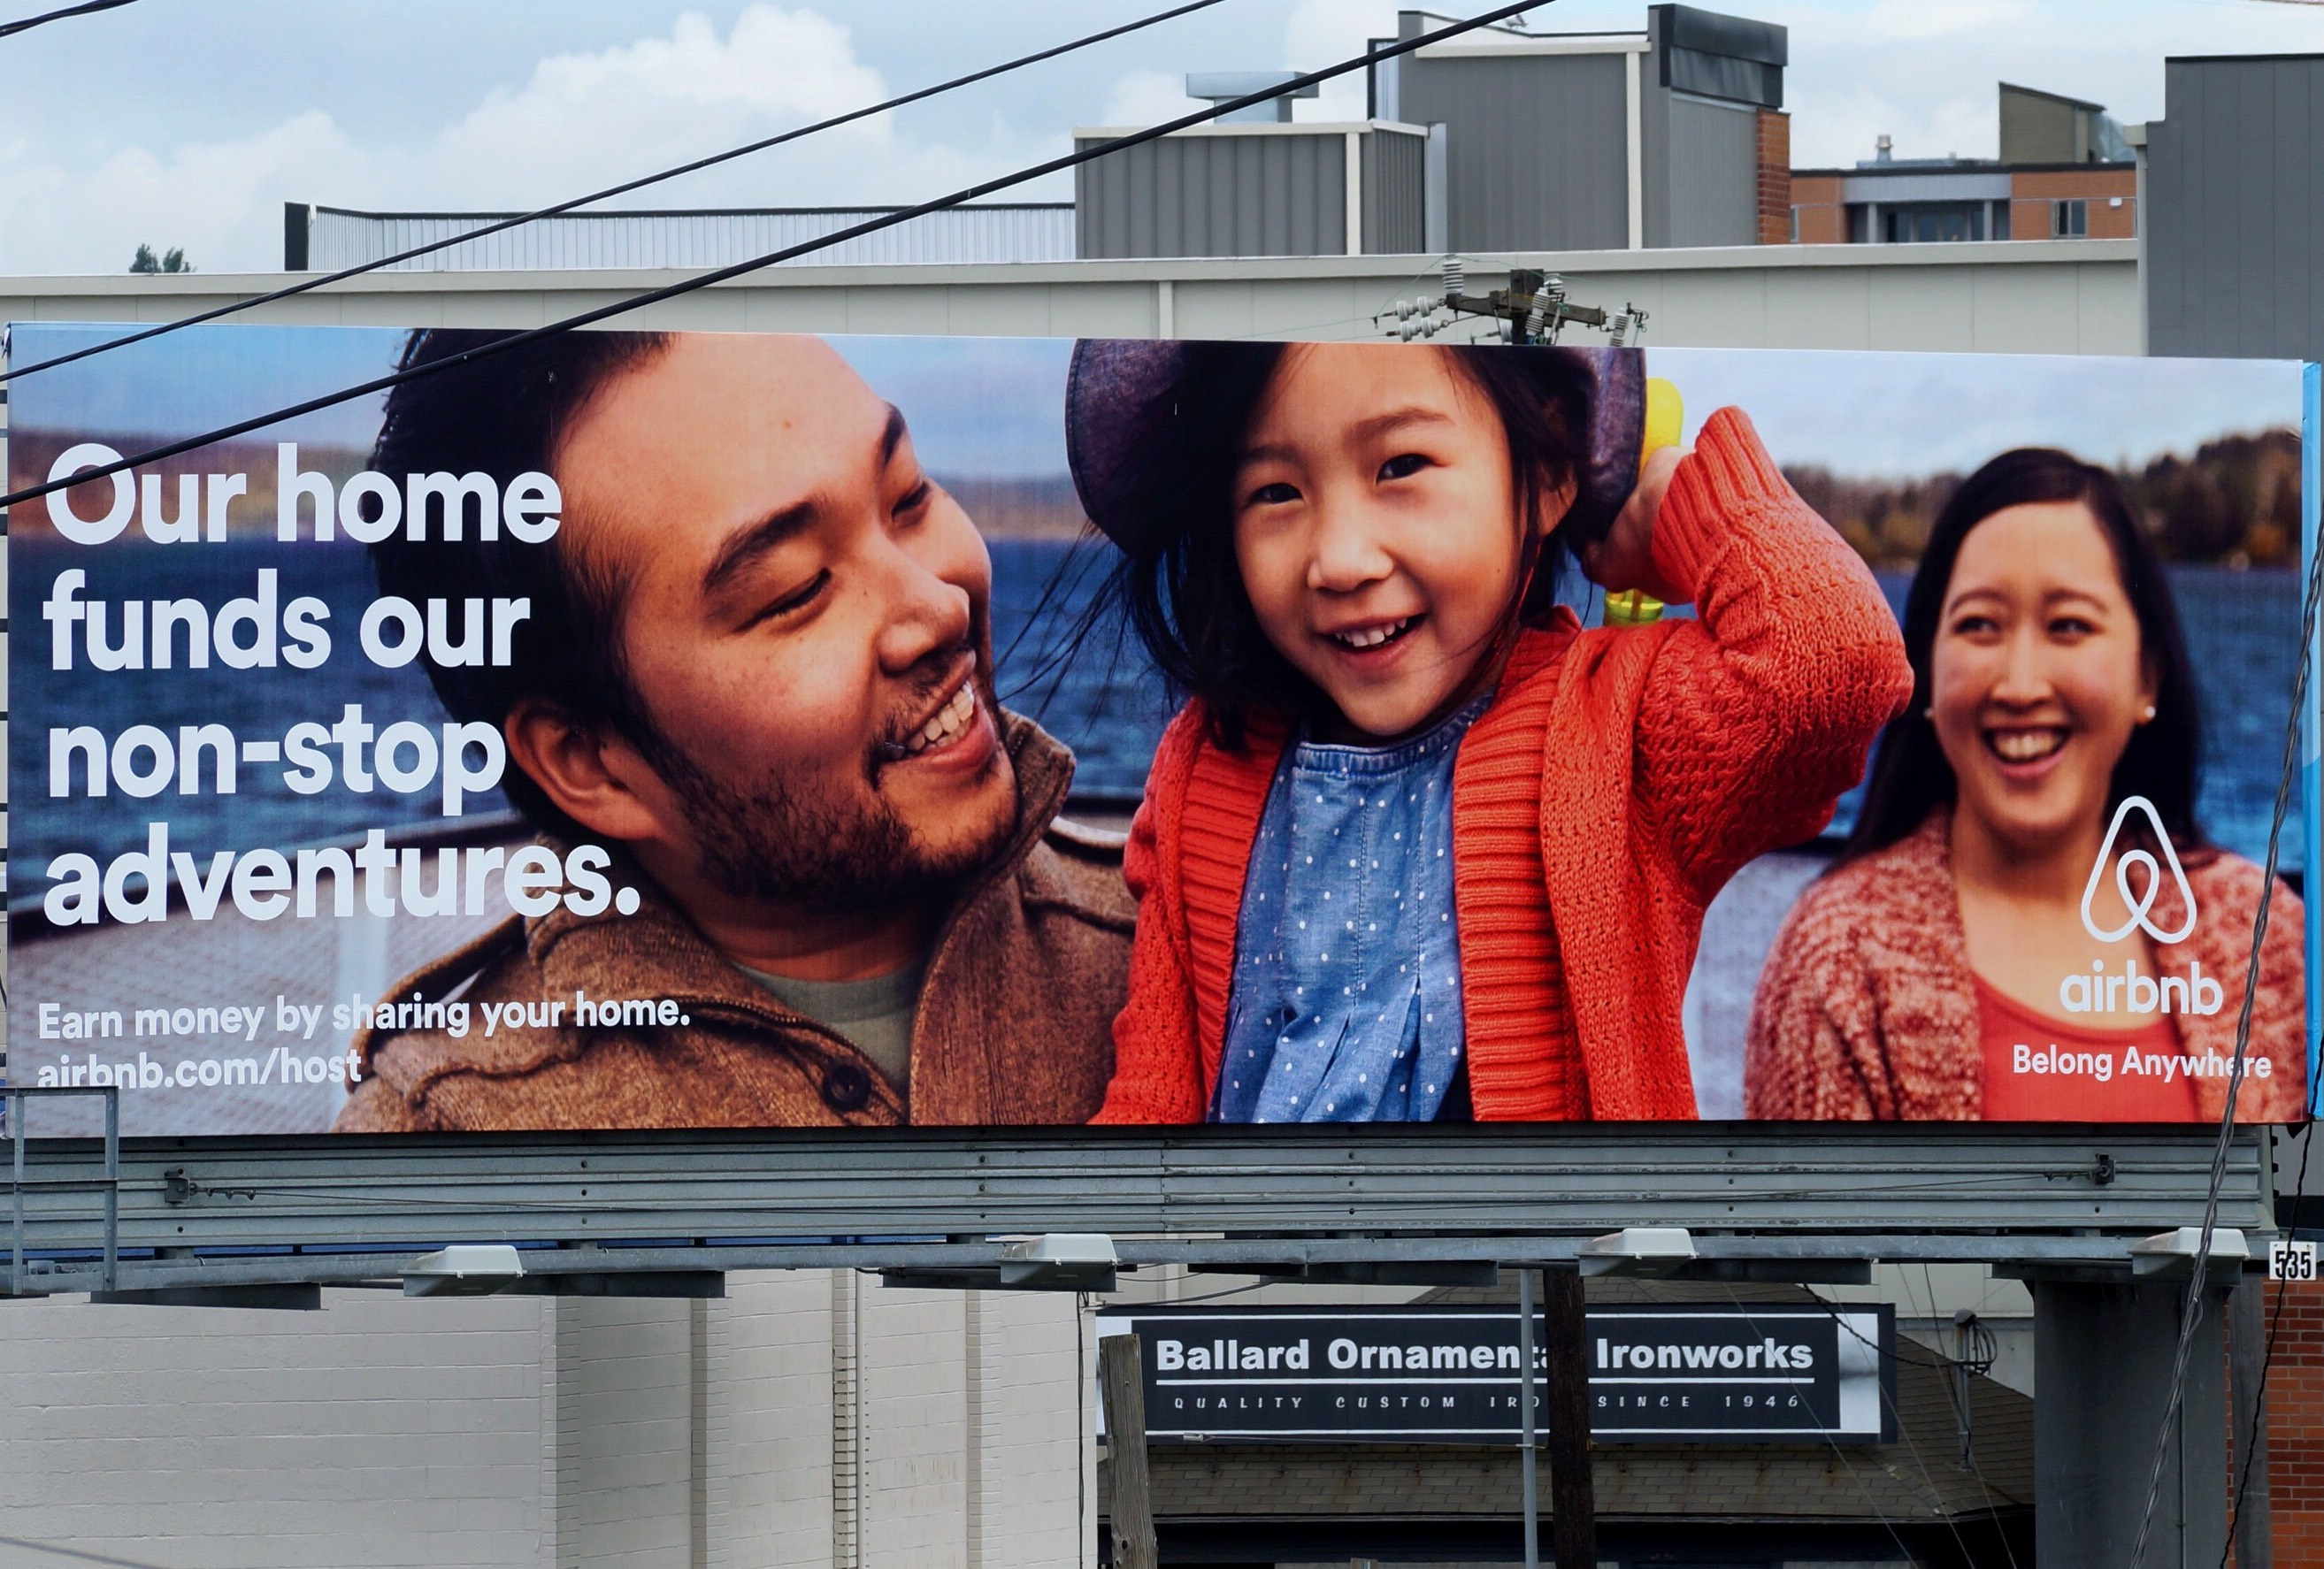
\includegraphics[width=\textwidth,scale=0.6]{images/airbnb.jpeg}
         \caption{}
         \label{fig:Airbib}
     \end{subfigure}
     \begin{subfigure}[b]{0.4\textwidth}
         \centering
         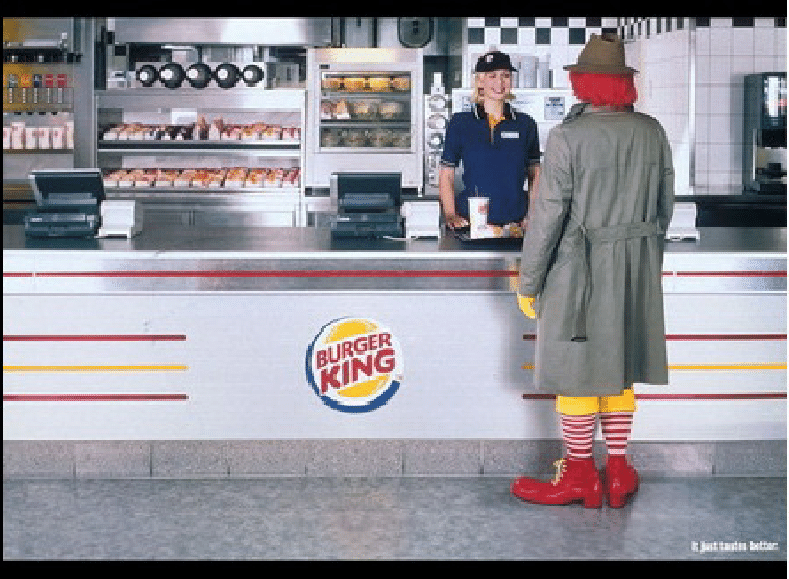
\includegraphics[width=\textwidth,scale=0.5]{images/Burger-King-vs-McDonalds-comparative-ad.png}
         \label{fig:mcdonald}
     \end{subfigure}
     \begin{subfigure}[b]{0.3\textwidth}
         \centering
         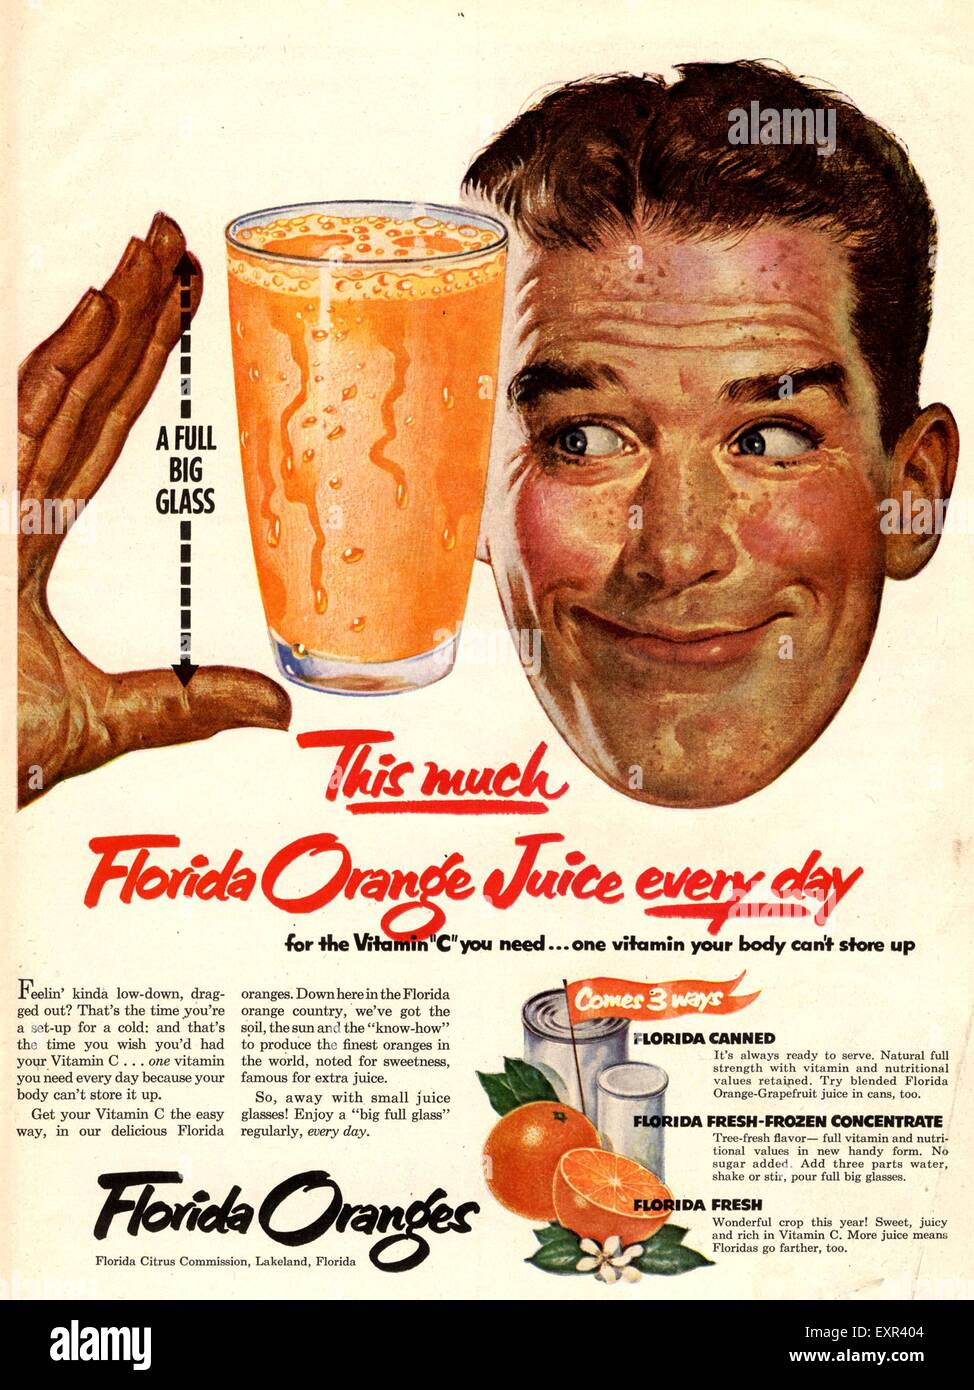
\includegraphics[width=\textwidth,scale=0.68]{images/1950s-usa-florida-orange-juice-magazine-advert-EXR404.jpeg}
         \label{fig:florida-juice}
     \end{subfigure}
     \begin{subfigure}[b]{0.3\textwidth}
         \centering
         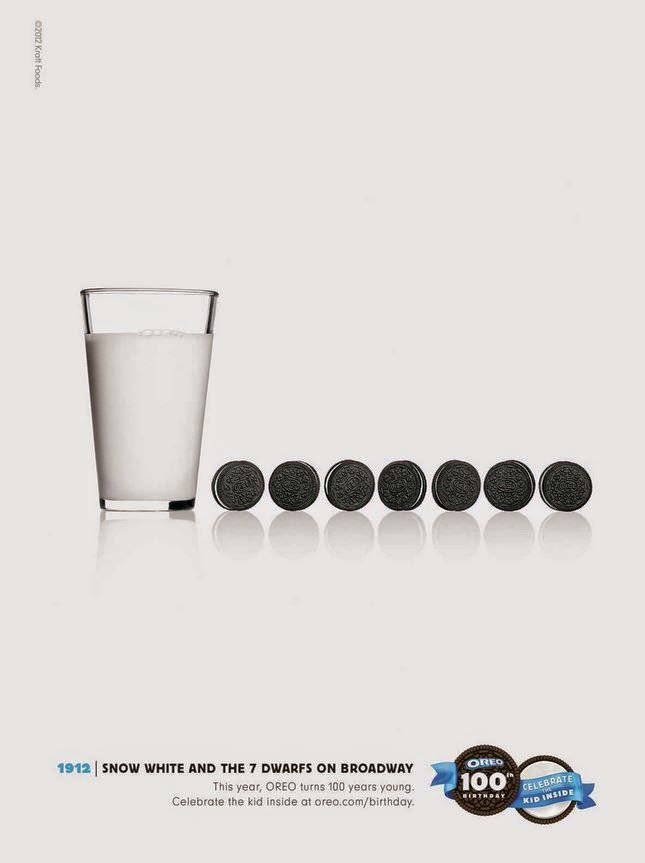
\includegraphics[width=\textwidth,scale=0.68]{images/Oreo_SnowWhite.jpeg}
         \label{fig:oreo}
     \end{subfigure}
     \begin{subfigure}[b]{0.6\textwidth}
         \centering
         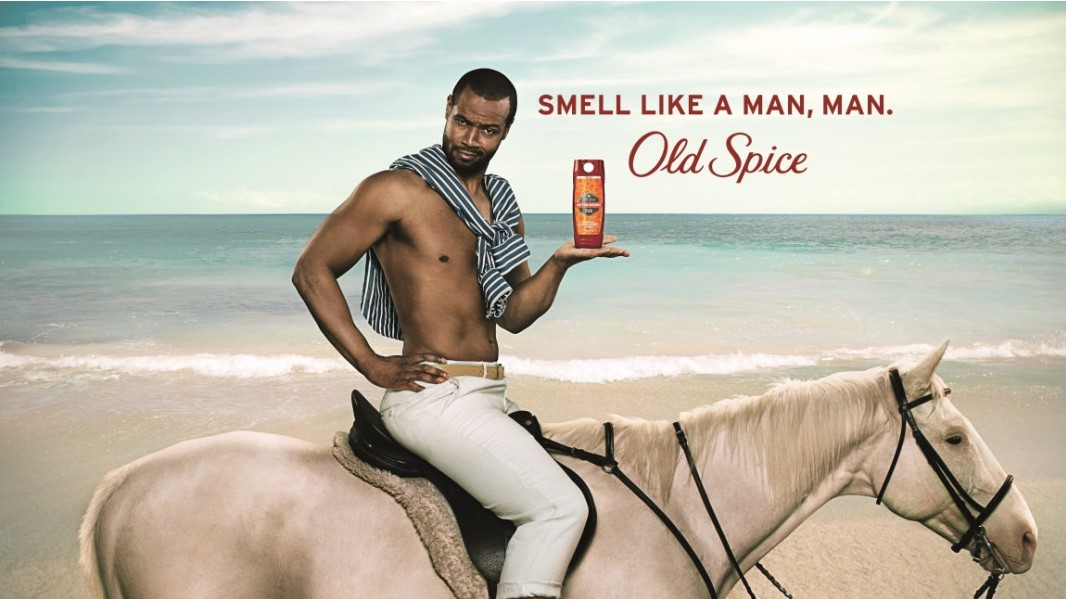
\includegraphics[width=\textwidth,scale=1.0]{images/old-spice.jpeg}
         \label{fig:old-spice}
     \end{subfigure}
     
    \caption{Example of various rhetoric strategies used in advertisements}
    \label{fig:rhetoric-strategies-ads}
\end{figure*}




Studying rhetorics of this form of communication is an essential part of understanding visual communication in marketing. Aristotle, in his seminal work on rhetoric, underlining the importance of persuasion, equated studying rhetorics with the study of persuasion\footnote{``Rhetoric may be defined as the faculty of discovering in any particular case all of the available means of \textit{persuasion}'' \cite{rapp2002aristotle}} \cite{rapp2002aristotle}. While persuasion is studied extensively in behavioral sciences, such as marketing \cite{meyers1999consumers,keller2003affect} and psychology \cite{hovland1953communication,petty1986elaboration}, computational modeling of persuasion in computer vision is still in its infancy, primarily due to the lack of benchmark datasets that can provide representative corpus to facilitate this line of research. In the limited work that has happened on persuasion in computer vision, researchers have tried to address the question of which image is more persuasive \cite{bai2021m2p2} or extracted low-level features (such as emotion, gestures, and facial displays), which indirectly help in identifying persuasion strategies without explicitly extracting the strategies themselves \cite{joo2014visual}. On the other hand, decoding persuasion in textual content has been extensively studied in natural language processing from both extractive, and generative contexts \cite{habernal2016makes,ChenYang2021,luu2019measuring}. This forms the motivation of our work, where we aim to identify the persuasion strategies used in visual content such as advertisements.




%In the limited work which has happened in computer vision domain for studying advertisements, researchers have investigated topics, sentiments, action-reason (containing \textit{what} the viewer should do and \textit{why} they should do it, according to the ad) statements \cite{hussain2017automatic,ye2018advise,ye2019interpreting}, or other features such as emotion, gestures, and facial display types in ads \cite{huang2016inferring,joo2014visual,DBLPconfbmvc0004K18}. While the prior computer vision work was important for finding the lower-level content properties of advertisements, studying advertisement rhetoric involves integrating the above lower-level elements to form \textit{persuasive message appeals}. %atkinson2019gets,carlile2018give,stab2014annotating,althoff2014ask,iyer2019unsupervised,rosenthal2017detecting,yang2019let,stab2017parsing,tan2016winning,wang-etal-2019-persuasion,zhang2016inferring,duerr2021persuasive,anand2011believe,chen2021weakly,hidey2017analyzing,he2018decoupling,durmus-cardie-2018-exploring,wachsmuth2017computational,longpre2019persuasion,shaikh-etal-2020-examining} use cases, and in  %




The systematic study of persuasion began in the 1920s with the media-effects research by Lasswell \cite{lasswell1971propaganda}, which was used as the basis for developing popular models of persuasion, like the Elaboration Likelihood Model (ELM) \cite{petty1986elaboration}, Heuristic Systematic Model (HSM) \cite{chaiken1980heuristic}, and Hovland's attitude change approach \cite{hovland1953communication}. %Amongst these, the most widely accepted model of persuasion theory is the Elaboration Likelihood Model (ELM). 
Laswell in this research broke down communication into five factors by defining communication as an act of \textit{who} said it, \textit{what} was said, in \textit{what} channel it was said, to \textit{whom} it was said, and with what \textit{effect} it was said. Later, this model was used as the basis for developing popular models of persuasion, like Elaboration Likelihood Model \cite{petty1986elaboration}, Heuristic Systematic Model \cite{chaiken1980heuristic}, and Hovland's attitude change approach \cite{hovland1953communication}. Amongst these, the most widely accepted model of persuasion theory is the Elaboration Likelihood Model (ELM). 

These models of persuasion posit a dual process theory that explains attitude and behavior change (persuasion) in terms of the following major factors: stimuli (messages), personal motivation (the desire to process the message), capability of critical evaluation, and cognitive busyness. These factors could be divided into cognitive, behavioral, and affective processes of attitude change. 
Thus, a person may begin liking a new political candidate because she just donated \$100 to the campaign (behavior-initiated change), because the theme music in a recently heard commercial induced a general pleasantness (affect-initiated change), or because the person was impressed with the candidate’s issue positions (cognitive initiated change). Similarly, if a person already likes a political candidate he may agree to donate money to the campaign (behavioral influence), may feel happiness upon meeting the candidate (affective influence), and may selectively encode the candidate’s issue positions (cognitive influence) \cite{petty1986elaboration}.

ELM posits that when facing a message from a persuader, the persuadee reacts by using the two information processing channels: central processing or peripheral processing. When the persuadee processes information centrally, the cognitive responses, or elaborations, will be much more relevant to the information, whereas when processing peripherally, the individual may rely on heuristics and other rules of thumb when elaborating on a message. The factors which influence how and how much one will elaborate the persuasive message is given by the message type, personal motivation, and other factors presented in the ELM. Being at the high end of the elaboration continuum, people assess object-relevant information in relation to schemas that they already possess, and arrive at a reasoned attitude that is supported by information \cite{van2011handbook}. 

In this chapter, we build on these psychological insights from persuasion models in sociology and marketing and study the message strategies that lead to persuasion. We codify, extend, and unify persuasion strategies studied in the psychology and marketing literature into a set of 20 strategies divided into 9 groups (see Fig.~\ref{fig:persuasion-strategies-headline-image}, Table~\ref{tab:persuasive-strategies-list}): \textit{Authority and Credibility}, \textit{Social Identity and Proof}, where cognitive indirection in the form of group decisioning and expert authority is used for decisions, \textit{Value and Impact Formulation} where logic is used to explain details and comparisons are made, \textit{Reciprocity}, \textit{Foot in the door}, \textit{Overcoming Resistance} where social and cognitive consistency norms are harnessed to aid decision-making, \textit{Scarcity}, \textit{Anthropomorphism} and \textit{Emotion} where information is evaluated from the lenses of feelings and emotions. In addition to introducing the most extensive vocabulary for persuasion strategies, we make a superset of persuasion strategies presented in the prior NLP works, which introduced text and domain-specific
persuasion tactics, thus making large-scale understanding of persuasion across multiple contexts comparable and replicable.


Constructing a large-scale dataset containing persuasion strategies labels is time-consuming and expensive. We leverage active learning to mitigate the cost of labeling fine-grained persuasion strategies in advertisements. We first introduce an attention-fusion model trained in a multi-task fashion over modalities such as text, image, and symbolism. We use the action-reason task from the Pitts Ads dataset \cite{hussain2017automatic} to train the model and then annotate the raw ad images from the same dataset for persuasion strategies based on an entropy based active learning technique.


%As an interesting use case, we extract 1600 raw ad images of Fortune-500 companies using the Facebook Ads API\footnote{\url{https://www.facebook.com/ads/library/api/}}. Then, using the model trained for persuasion strategies, we labelled and analyzed the advertisement campaigns on different companies and industry segments. We find that (\S\ref{sec:Case Study}).


To sum up, our contributions include:\\
1. We construct the largest set of generic persuasion strategies based on theoretical and empirical studies in marketing, social psychology, and machine learning literature. \\
2. We introduce the first dataset for studying persuasion strategies in advertisements. This enables initial progress on the challenging task of automatically understanding the messaging strategies conveyed through visual advertisements. We also construct a prototypical dataset containing image segmentation masks annotating persuasion strategies in different segments of an image.\\
3. We formulate the task of predicting persuasion strategies with a multi-task attention fusion model.\\
4. We conduct extensive experiments on the released corpus,
showing the effect of different modalities on identifying persuasion
strategies, correlation between strategies and topics
and objects with different strategies.\\

\subsection{Related Work}
\label{sec:related work-persuasion}


\textit{How do messages change people's beliefs and actions?} The systematic study of persuasion has captured researchers’ interest since the advent of mass influence mechanisms such as radio, television, and advertising. Work in persuasion spans across multiple fields, including psychology, marketing, and machine learning. 


\textbf{Persuasion in Marketing and Social Psychology:} Sociology and communication science has studied persuasion for centuries now starting from the seminal work of Aristotle on rhetoric. Researchers have tried to construct and validate models of persuasion. Due to space constraints, while we cannot cover a complete list of literature, in Section~\ref{tab:persuasive-strategies-list}, we list the primary studies which originally identified the presence and effect of various persuasion tactics on persuadees. We build on almost a century of this research and crystallize them into the persuasion strategies we use for annotation and modeling. %Using both expenditure and income calculations, \citet{mccloskey1995one} calculate that roughly one quarter of the US GDP in 1994 was due to persuasion. 
Any instance of (successful) persuasion is composed of two events: (a) an attempt by the persuader, which we term as the persuasion strategies, and (b) subsequent uptake and response by the persuadee \cite{anand2011believe,vakratsas1999advertising}. In this work, we study (a) only while leaving (b) for future work. Throughout the rest of the paper, when we say persuasion strategy, we mean the former without considering whether the persuasion was successful or not. 




\begin{landscape}
    \pagestyle{landscapeStyle}
\begin{figure*}[t]
% \vspace*{-12mm}
        \centering
        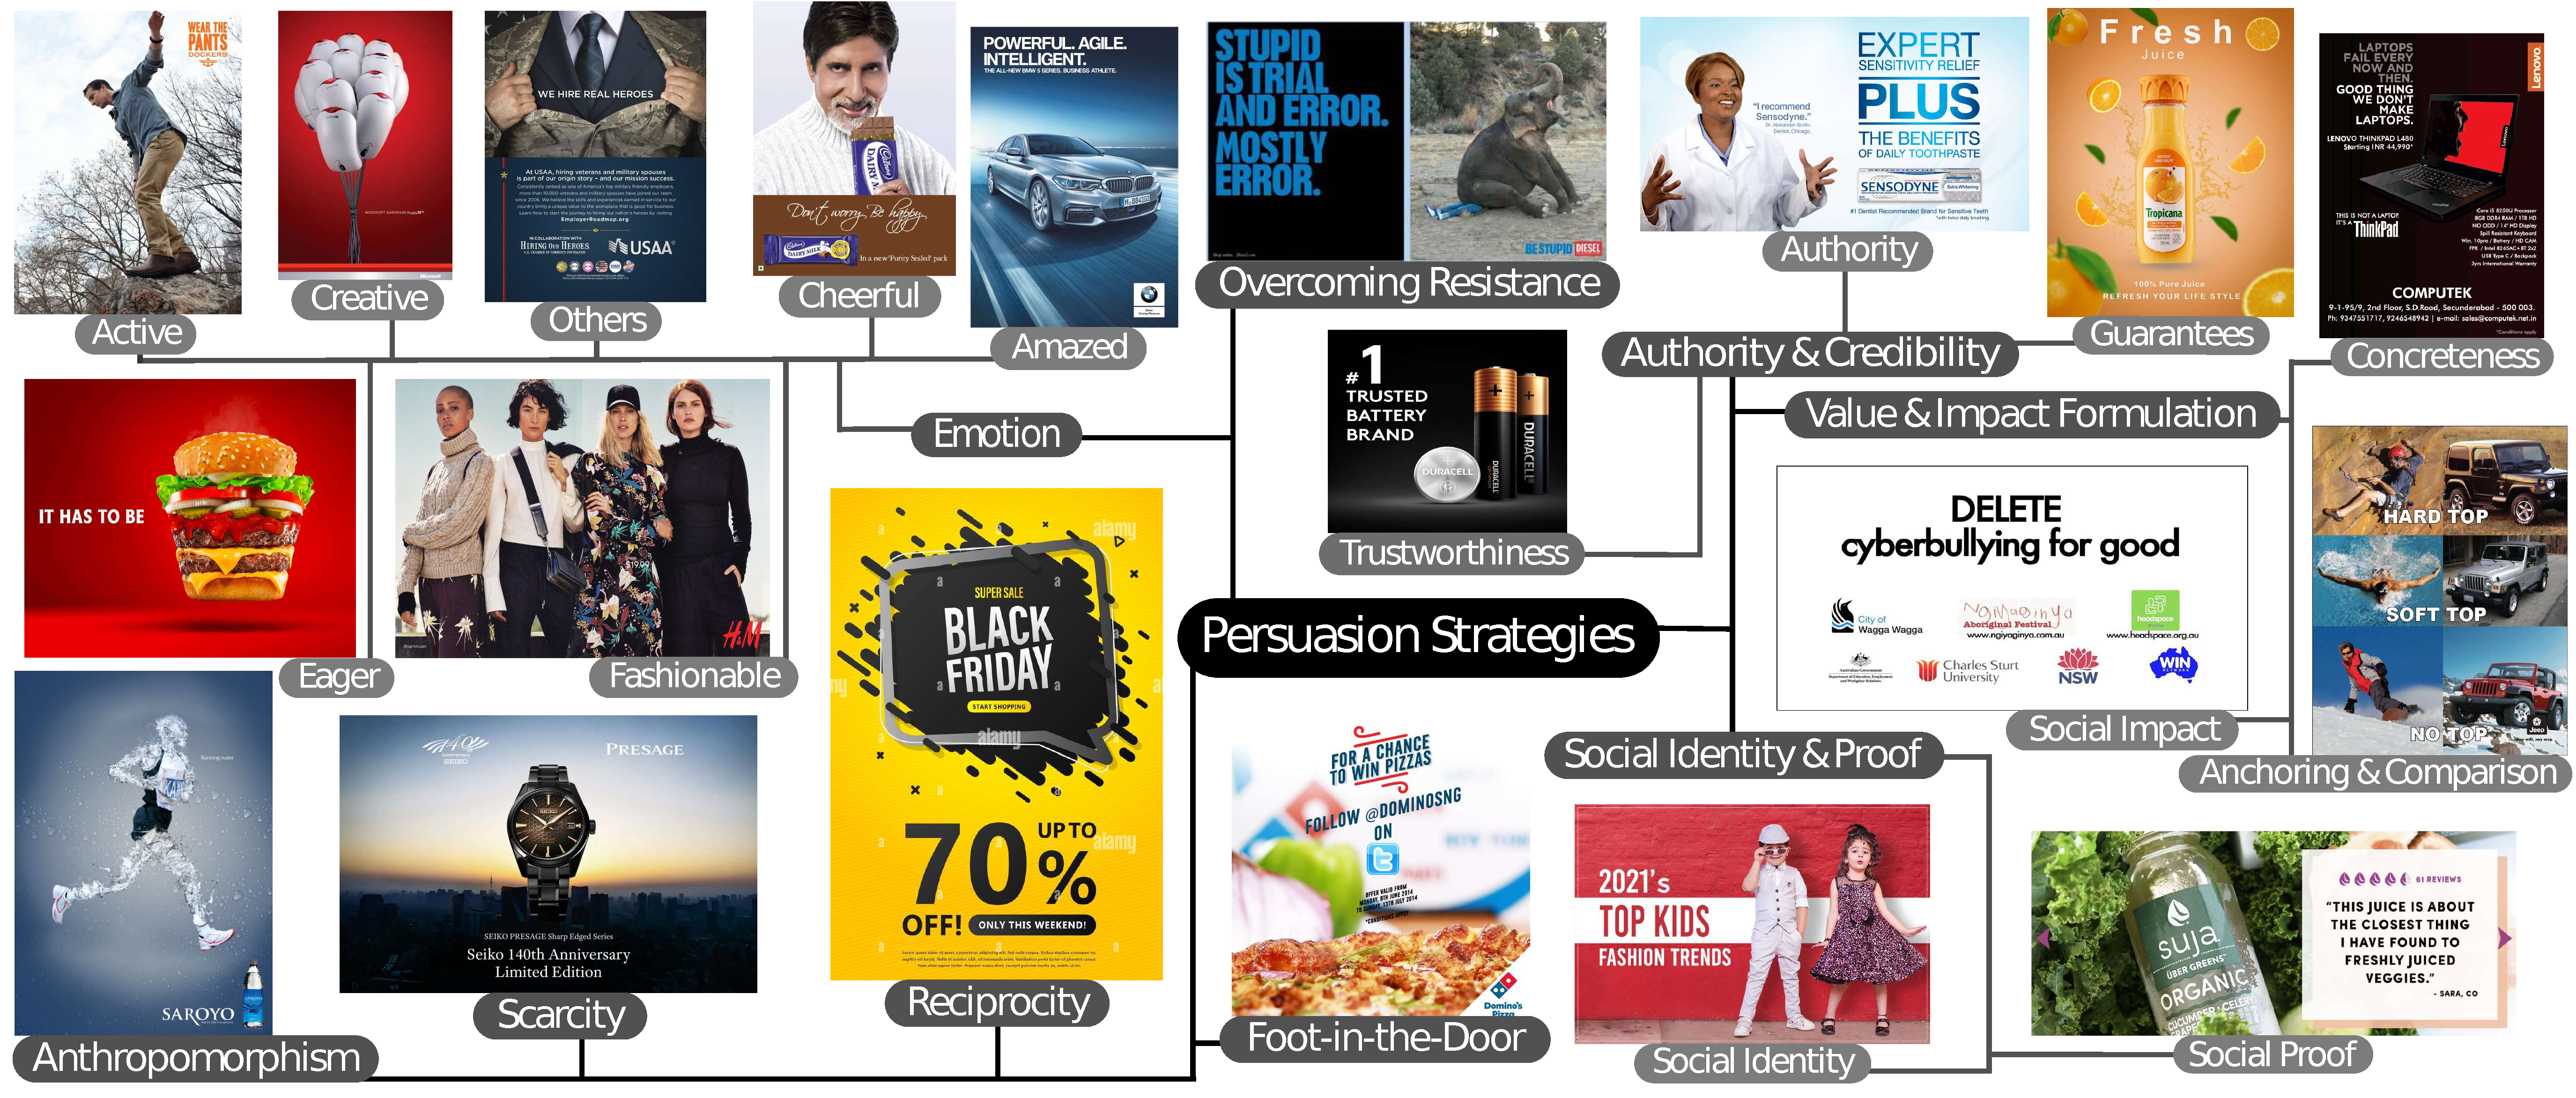
\includegraphics[width=1.5\textwidth]{images/flowchart.pdf}
        \caption{\small \looseness=-1 Persuasion strategies in advertisements. Marketers use both text and vision modalities to create ads containing different messaging strategies. Different persuasion strategies are constituted by using various rhetorical devices such as slogans, symbolism, colors, emotions, allusion.}
        \label{fig:persuasion-strategies-headline-image}
% \vspace*{-4mm}
\end{figure*}
\end{landscape}





\textbf{Persuasion in Machine Learning:} Despite extensive work in social psychology and marketing on persuasion, most of the work is qualitative, where researchers have looked at a small set of messages with various persuasion strategies to determine their effect on participants. Computational modeling of persuasion is still largely lacking. In the limited work in computational modeling of persuasion, almost all of it is concentrated in the NLP literature, with only very few works in computer vision.
Research on persuasion in NLP under the umbrella of argumentation mining is broadly carried out from three perspectives: extracting persuasion tactics, studying the effect of constituent factors on persuasion, and measurement of persuasiveness nature of content. A few examples of research studies that annotate persuasive strategies in various forms of persuader-persuadee interactions like discussion forums, social media, blogs, academic essays, and debates are \cite{anand2011believe,tan2016winning,chen2021weakly}. We use these and other studies listed in Section~\ref{tab:persuasive-strategies-list} to construct our vocabulary of persuasion strategies in advertisements. 

Other studies focus on factors such as argument ordering \cite{shaikh-etal-2020-examining,li-etal-2020-exploring-role}, target audience \cite{lukin-etal-2017-argument}, and prior beliefs \cite{el-baff-etal-2020-analyzing} for their effect in bringing about persuasion. Studies such as \cite{althoff2014ask,wei2016post} also try to measure persuasiveness and generate persuasive content. The generation of persuasive (textual) messages has been studied \cite{donadello2020explaining} and, in particular, a novel ML method for learning user model tailored persuasion strategy has also been proposed \cite{hadoux2021strategic, donadello2022machine}.



As one of the first works in the limited work in the computer vision domain, Joo \textit{et al.} \cite{joo2014visual} introduced syntactical and intent features such as facial displays, gestures, emotion, and personality, which result in persuasive images. Their analysis was done on human images, particularly politicians, during their campaigns. %\citet{huang2016inferring} built on top of their dataset to improve their results by using finetuned CNNs. 
Their work on political campaigners is more restrictive than general product and public-service advertisements. Moreover, they deal with low-level features such as gestures and personality traits depicted through the face, which are important for detecting persuasion strategies but are not persuasion strategies themselves. Recently, Bai \textit{et al.} \cite{bai2021m2p2} studied persuasion in debate videos where they proposed two tasks: debate outcome prediction and intensity of persuasion prediction. Through these tasks, they predict the persuasiveness of a debate speech, which is orthogonal to the task of predicting the strategy used by the debater. Other similar works which discuss persuasiveness of images and videos are \cite{joo2015automated,siddiquie2015exploiting}.


%\noindent \textbf{Active Learning} tackles the problem of selecting samples from unlabeled sets to be annotated by an oracle. In the last decade, several active learning strategies have been proposed and applied to several research fields, including speech recognition \cite{hakkani2002active}, natural language processing \cite{thompson1999active}, chemistry \cite{duros2017human}. We refer the reader to the survey of \citet{settles2009active} for an extensive review of active learning methods. Many studies including \citet{collins2008towards,miller_linder_mebane_2020,mullapudi2021learning} have practically applied active learning to annotate datasets and shown substantial improvement in labelling budget and time. 




\subsection{Generic Taxonomy of Persuasion Strategies}
\label{tab:persuasive-strategies-list}
This section introduces the generic taxonomy of persuasive strategies, their definitions, examples, and connections with prior work. Representative literature from a)~\texttt{SPM}: Social Psychology and Marketing, b)~\texttt{ML}: Machine Learning

\begin{enumerate}
    \item Authority and Credibility: \texttt{SPM}:\cite{aronson1963communicator,milgram1978obedience,cialdini2007influence,milgram1963behavioral,mcginnies1980better,giffin1967contribution,petty1986elaboration} \texttt{ML}:\cite{anand2011believe,iyer2019unsupervised,wachsmuth2017computational,ChenYang2021,durmus-cardie-2018-exploring}
    \begin{enumerate}
        \item \textbf{Guarantees}: Guarantees reduce risk and people try out such products more often. 

        \item \textbf{Authority}: Authority indicated through expertise, source of power, third-party approval, credentials, and awards
    
        \item \textbf{Trustworthiness}: Trustworthiness indicated honesty and integrity of the source through tropes like years of experience, ``trusted brand'', numbers and statistics
    \end{enumerate}

    \item Social Identity and Proof: \texttt{SPM}:\cite{deutsch1955study,petty1997attitudes,wood2000attitude,cialdini2004social,levesque2020human} \texttt{ML}: \cite{anand2011believe,iyer2019unsupervised,rosenthal2017detecting,yang2019let,zhang2016inferring,stab2017parsing,althoff2014ask,hidey2017analyzing,durmus-cardie-2018-exploring}

    \begin{enumerate}
        \item \textbf{Social Identity}: \textit{Normative} influence, which involves conformity with the positive expectations of ``another'', who could be ``another person, a group, or one's self'' (includes self-persuasion, fleeting attraction, alter-casting, and exclusivity)

        \item \textbf{Social Proof}: \textit{Informational influence} by accepting information obtained from others as evidence about reality, \textit{e.g.}, customer reviews and ratings 
    \end{enumerate}

    \item  Reciprocity: \texttt{SPM}:\cite{regan1971effects,cialdini2007influence,clark1984record,clark1979interpersonal,clark1986keeping} \texttt{ML}:\cite{anand2011believe,iyer2019unsupervised,althoff2014ask,ChenYang2021,shaikh-etal-2020-examining}
    \begin{enumerate}
        \item \textbf{Reciprocity}: By \textit{obligating} the recipient of an act to repayment in the future, the rule for reciprocation begets a sense of future obligation, often unequal in nature
    \end{enumerate}

    \item Foot in the door: \texttt{SPM}: \cite{freedman1966compliance,burger1999foot,cialdini2007influence} \texttt{ML}:\cite{chen2021weakly,wang-etal-2019-persuasion,vargheese2020exploring}
    \begin{enumerate}
        \item \textbf{Foot in the door}: Starting with small requests followed by larger requests to facilitate compliance while maintaining \textit{cognitive coherence}.
    \end{enumerate}

    \item  Overcoming Resistance: \texttt{SPM}:\cite{mcguire1961relative,knowles2004resistance,mcguire1964inducing} \texttt{ML}:\{None\}
    \begin{enumerate}
        \item \textbf{Overcoming Resistance}: Overcoming resistance (reactance) by postponing consequences to the future, by focusing resistance on realistic concerns, by forewarning that a message will be coming, by acknowledging resistance, by raising self-esteem and a sense of efficacy. 
    \end{enumerate}


    \item  Value and Impact Formulation: \texttt{SPM}:\cite{lee2010value,furnham2011literature,wegener2001implications,tversky1974judgment,strack1997explaining,bhattacharya2003consumer} \texttt{ML}:\cite{zhang2017characterizing,longpre2019persuasion}
    \begin{enumerate}
        \item \textbf{Concreteness}: Using concrete facts, evidence, and statistics to appeal to the logic of consumers 

        \item \textbf{Anchoring and Comparison}: A product's value is strongly influenced by what it is compared to.

        \item \textbf{Social Impact}: Emphasizes the importance or bigger (societal) impact of a product 
    \end{enumerate}

    \item Scarcity: \texttt{SPM}: \cite{brehm1966theory,lynn1991scarcity,rothman1999systematic,tversky1985framing} \texttt{ML}:\cite{yang2019let,ChenYang2021,shaikh-etal-2020-examining}
    \begin{enumerate}
        \item \textbf{Scarcity}: People assign more value to opportunities when they are less available. This happens due to psychological reactance of losing freedom of choice when things are less available or they use availability as a cognitive shortcut for gauging quality. 
    \end{enumerate}

    \item Anthropomorphism: \texttt{SPM}:\cite{fournier1998consumers,levesque2020human,epley2007seeing} \texttt{ML}:\{None\}
    \begin{enumerate}
        \item \textbf{Anthropomorphism}: When a brand or product is seen as human-like, people will like it more and feel closer to it.
    \end{enumerate}

    \item Emotion: Aesthetics, feeling and other non-cognitively demanding features used for persuading consumers \texttt{SPM}:\cite{hibbert2007guilt,petty1986elaboration,petty1983central}\\\texttt{ML}:\cite{yang2019let,tan2016winning,hidey2017analyzing,he2018decoupling,durmus-cardie-2018-exploring,zhang2017characterizing,wachsmuth2017computational}
    \begin{enumerate}
        \item \textbf{Amazed}
        \item \textbf{Fashionable}
        \item \textbf{Active, Eager}
        \item \textbf{Feminine}
        \item \textbf{Creative}
        \item \textbf{Cheerful}
        \item \textbf{Further Minor}
    \end{enumerate}

    \item \textbf{Unclear}: If the ad strategy is unclear     
\end{enumerate}

%%%%%%%%%%%%%%%%%%%%%%%%%%%%%%%%%%%%%%%%%%%%%%%%%%%%
%%%%%%%%%%%%%%%%%%%%%%%%%%%%%%%%%%%%%%%%%%%%%%%%%%%%
%%%%%%%%%%%%%%%%%%%%%%%%%%%%%%%%%%%%%%%%%%%%%%
%%%%%%%%%%%%%%%%%%%%%%%%%%%%%%%%%%%%%%%%%%%%%%


% \vspace{-2mm}
\subsection{Persuasion Strategy Corpus Creation}
\label{sec:Persuasion Strategy Corpus Creation}

\begin{figure}[t]
% \vspace{-10mm}
        \centering
        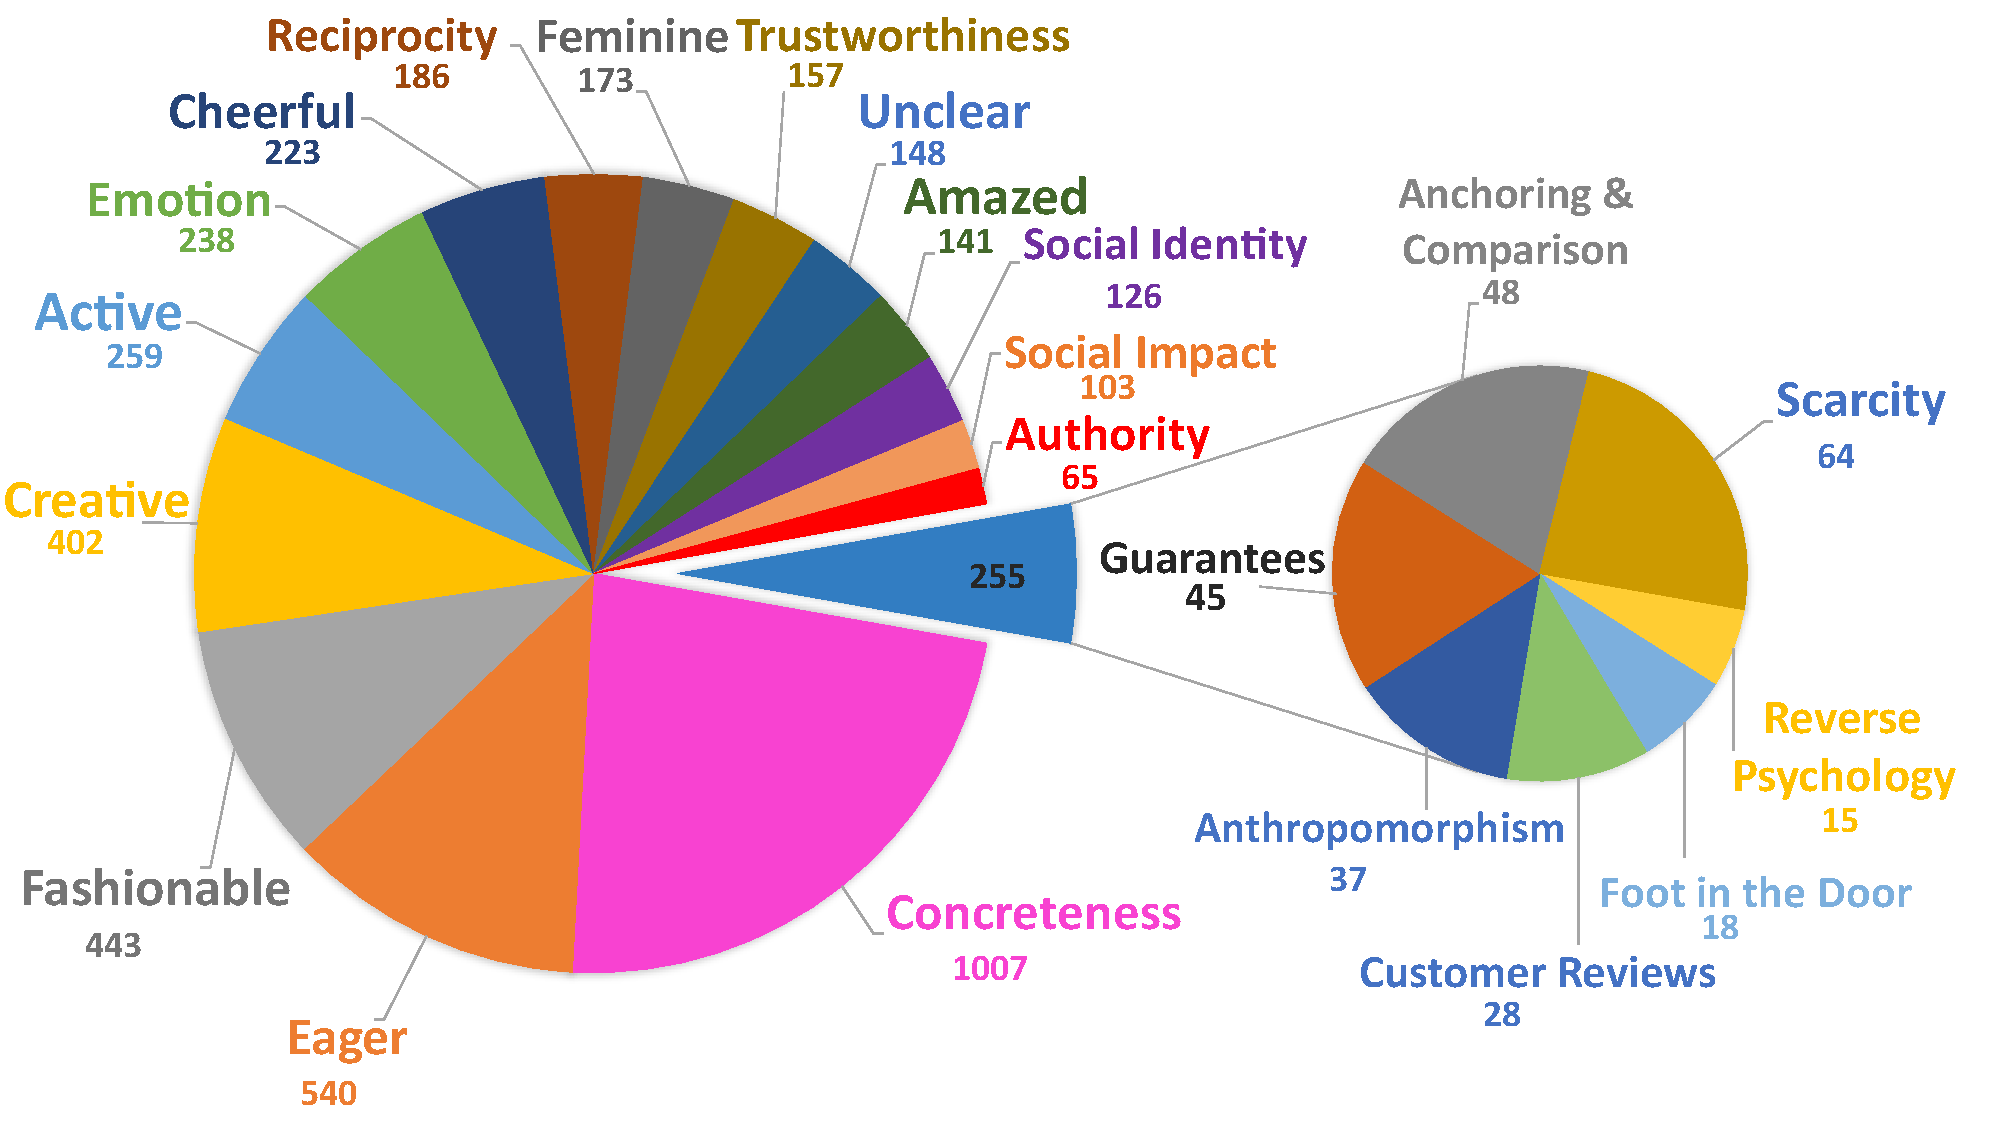
\includegraphics[scale=0.3]{images/pie_chart.pdf}
        \caption{Distribution of Persuasion Strategies in the image persuasion strategy dataset. The top-3 strategies are Concreteness, Eager, and Fashionable. \small}
        \label{fig:persuasion-strategies-distribution}
        % \vspace{-4mm}
    \end{figure}


\subsubsection{Persuasion Strategy Dataset For Image Advertisements}

To annotate persuasion strategies on image advertisements, we leverage raw images from the Pitts Ads dataset. It contains 64,832 image ads with labels of topics, sentiments, symbolic references (\textit{e.g.} dove symbolizing peace), and reasoning the ad provides to its viewers (see Fig~\ref{fig:preds-sup} for a few examples). The dataset had ads spanning multiple industries, products, services, and also contained public service announcements. Through this, they presented an initial work for the task of understanding visual rhetoric in ads. Since the dataset already had a few types of labels associated with the ad images, we used active learning on a model trained in a multi-task learning fashion over the reasoning task introduced in their paper. We explain the model and then the annotation strategy followed in \S\ref{sec:Persuasion Strategy Prediction Model}. 







To commence training, we initially annotated a batch of $250$ randomly selected ad images with persuasion strategies defined in Section~\ref{tab:persuasive-strategies-list}. We recruited four research assistants to label persuasion strategies for each advertisement. Definitions and examples of different persuasion strategies were provided, together with a training session where we asked annotators to annotate a number of example images and walked them through any disagreed annotations. To assess the reliability of the annotated labels, we then asked them to annotate the same 500 images and computed Cohen's Kappa statistic to measure inter-rater reliability. We obtained an average score of 0.55. The theoretical maximum of Kappa, given the unequal distribution, is 0.76. In such cases, Cohen \cite{cohen1960coefficient} suggested that one should divide kappa by its maximum value $\mathbf{k}/\mathbf{k_{max}}$, which comes out to be 0.72. This is a \textit{substantial} agreement. Further, to maintain labeling consistency, each image was double annotated, with all discrepancies resolved by an intervention of the third annotator using a majority vote. 


The assistants were asked to label each image with no more than 3 strategies. If an image had more than 3 strategies, they were asked to list the top 3 strategies according to the area covered by the pixels depicting that strategy. In total, we label 3000 ad-images with their persuasion strategies; and the number of samples in train, val, and test split are 2500, 250, and 250, respectively\footnote{Table~\ref{table:strategy-train-test-val-stats} shows the detailed distribution of the number of strategies in ads}. Fig.~\ref{fig:persuasion-strategies-distribution} presents the distribution of persuasion strategies in the dataset. It is observed that concreteness is the most used strategy in the dataset, followed by eagerness and fashion. The average number of strategies in an ad is 1.49, and the standard deviation is 0.592. We find that scarcity (92.2\%), guarantees (91.1\%), reciprocity (84.4\%), social identity (83.3\%), and cheerful (83\%), %and anchoring and comparison (77.1\%), trustworthiness (75.8\%), social proof (75\%),  amazed (73.1\%) and concreteness (70.3\%) 
are the top 5 strategies, which occur in groups of 2 or 3. We observe that the co-occurrence of these strategies is due to the fact that many of them cover only a single modality (\textit{i.e.}, text or visual), leaving the other modality free for a different strategy. For example, concreteness is often indicated by illustrating points in text, while the visual modality is free for depicting, say, emotion. See Fig.~\ref{fig:segmented image} for an example, where the image depicting \textit{Authority} also has concreteness strategy in it. Similarly, feminine emotion is also depicted in Fig.~\ref{fig:footwear-strategies}, along with concreteness.


\begin{figure*}[!h]
    % \vspace{-4mm}
    \centering
    \begin{subfigure}[b]{0.4\textwidth}
        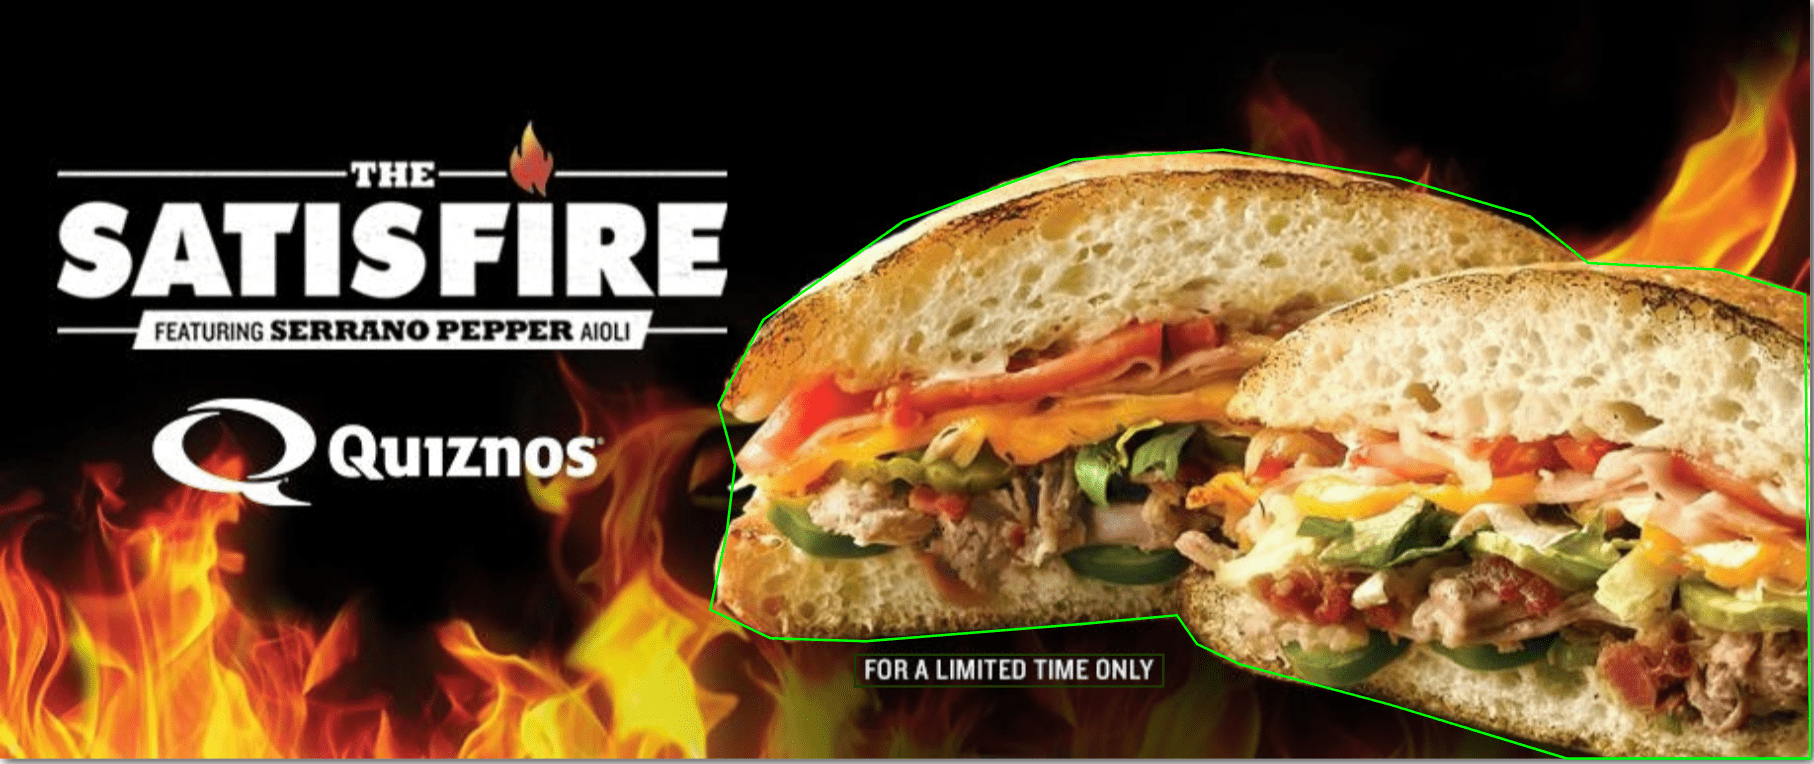
\includegraphics[scale=0.2]{images/Image1.png}
    \end{subfigure}
    \begin{subfigure}[b]{0.4\textwidth}
        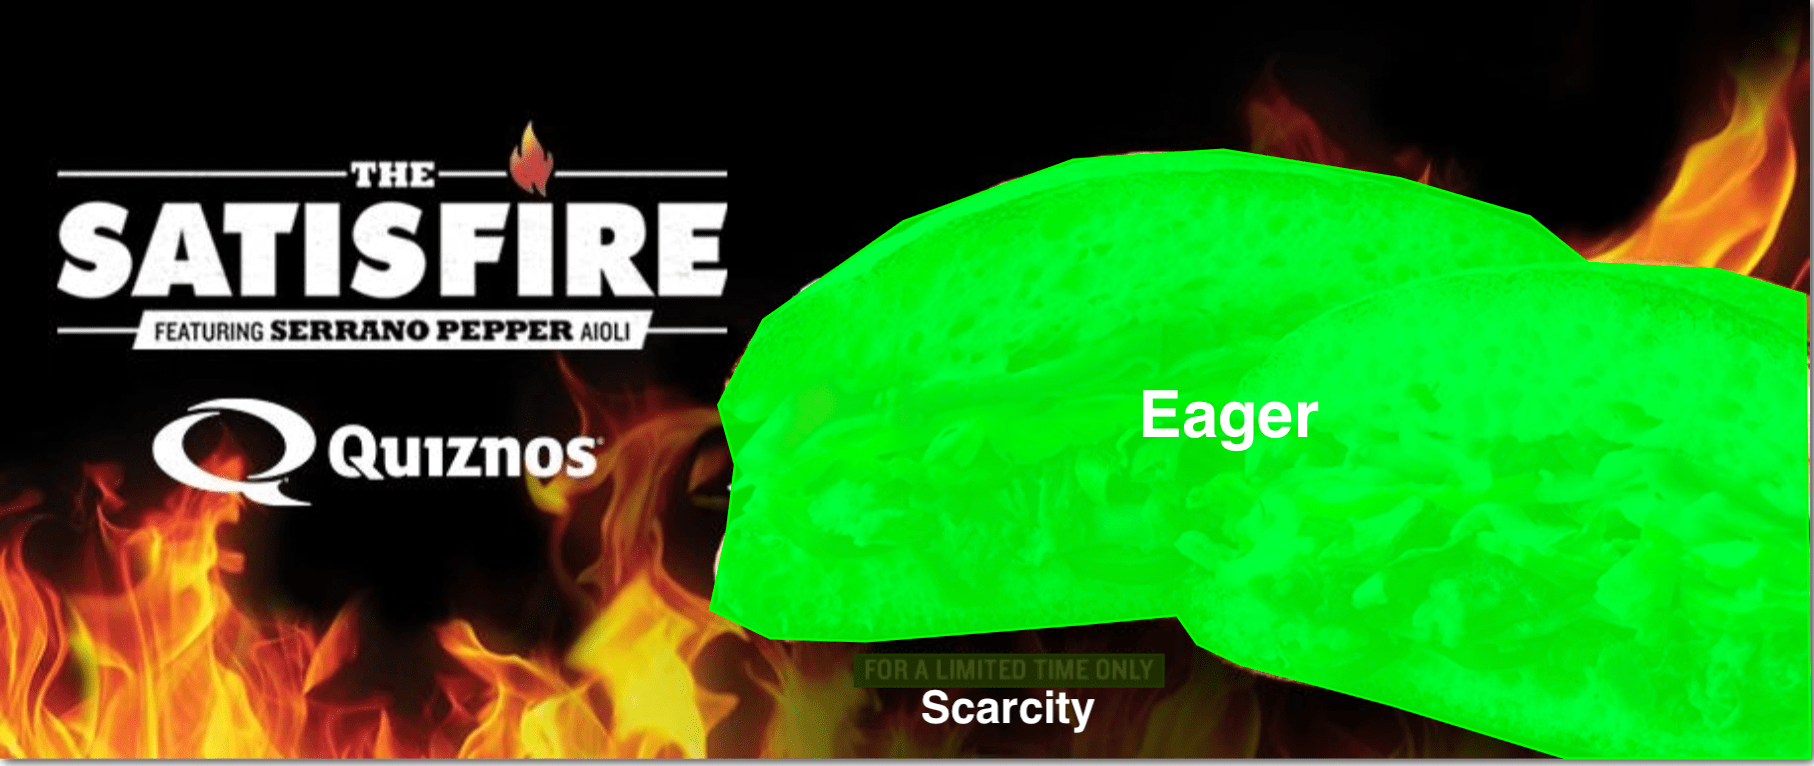
\includegraphics[scale=0.2]{images/Image1_Segment.png}



    \end{subfigure}
     \begin{subfigure}[b]{0.245\textwidth}
         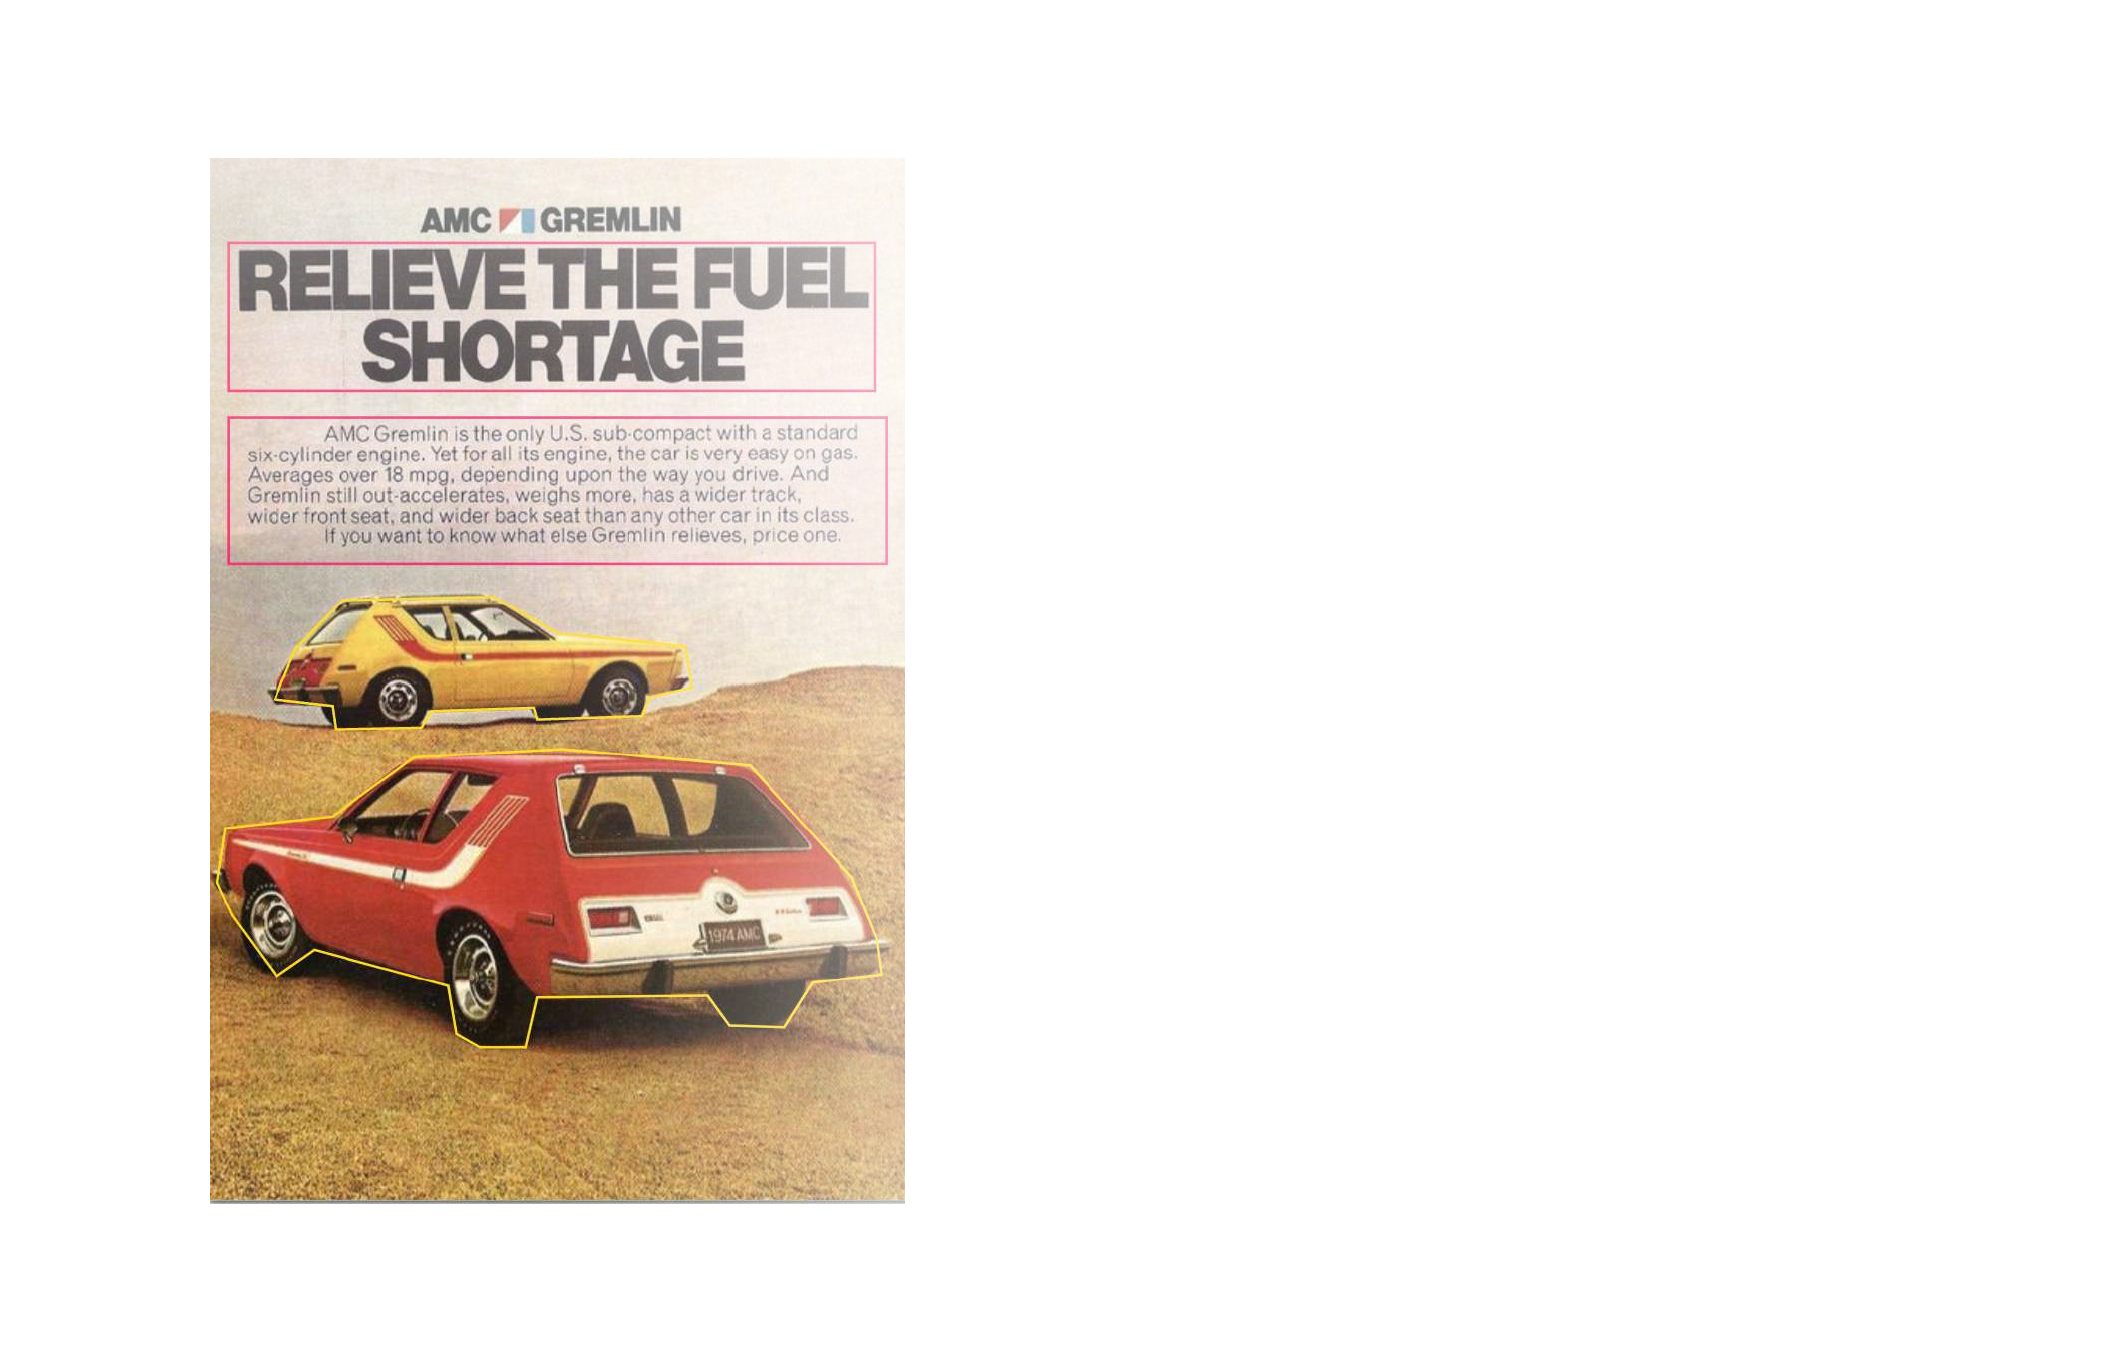
\includegraphics[scale=0.22]{images/fuel-shortage-original.pdf}
     \end{subfigure}
     \begin{subfigure}[b]{0.245\textwidth}
         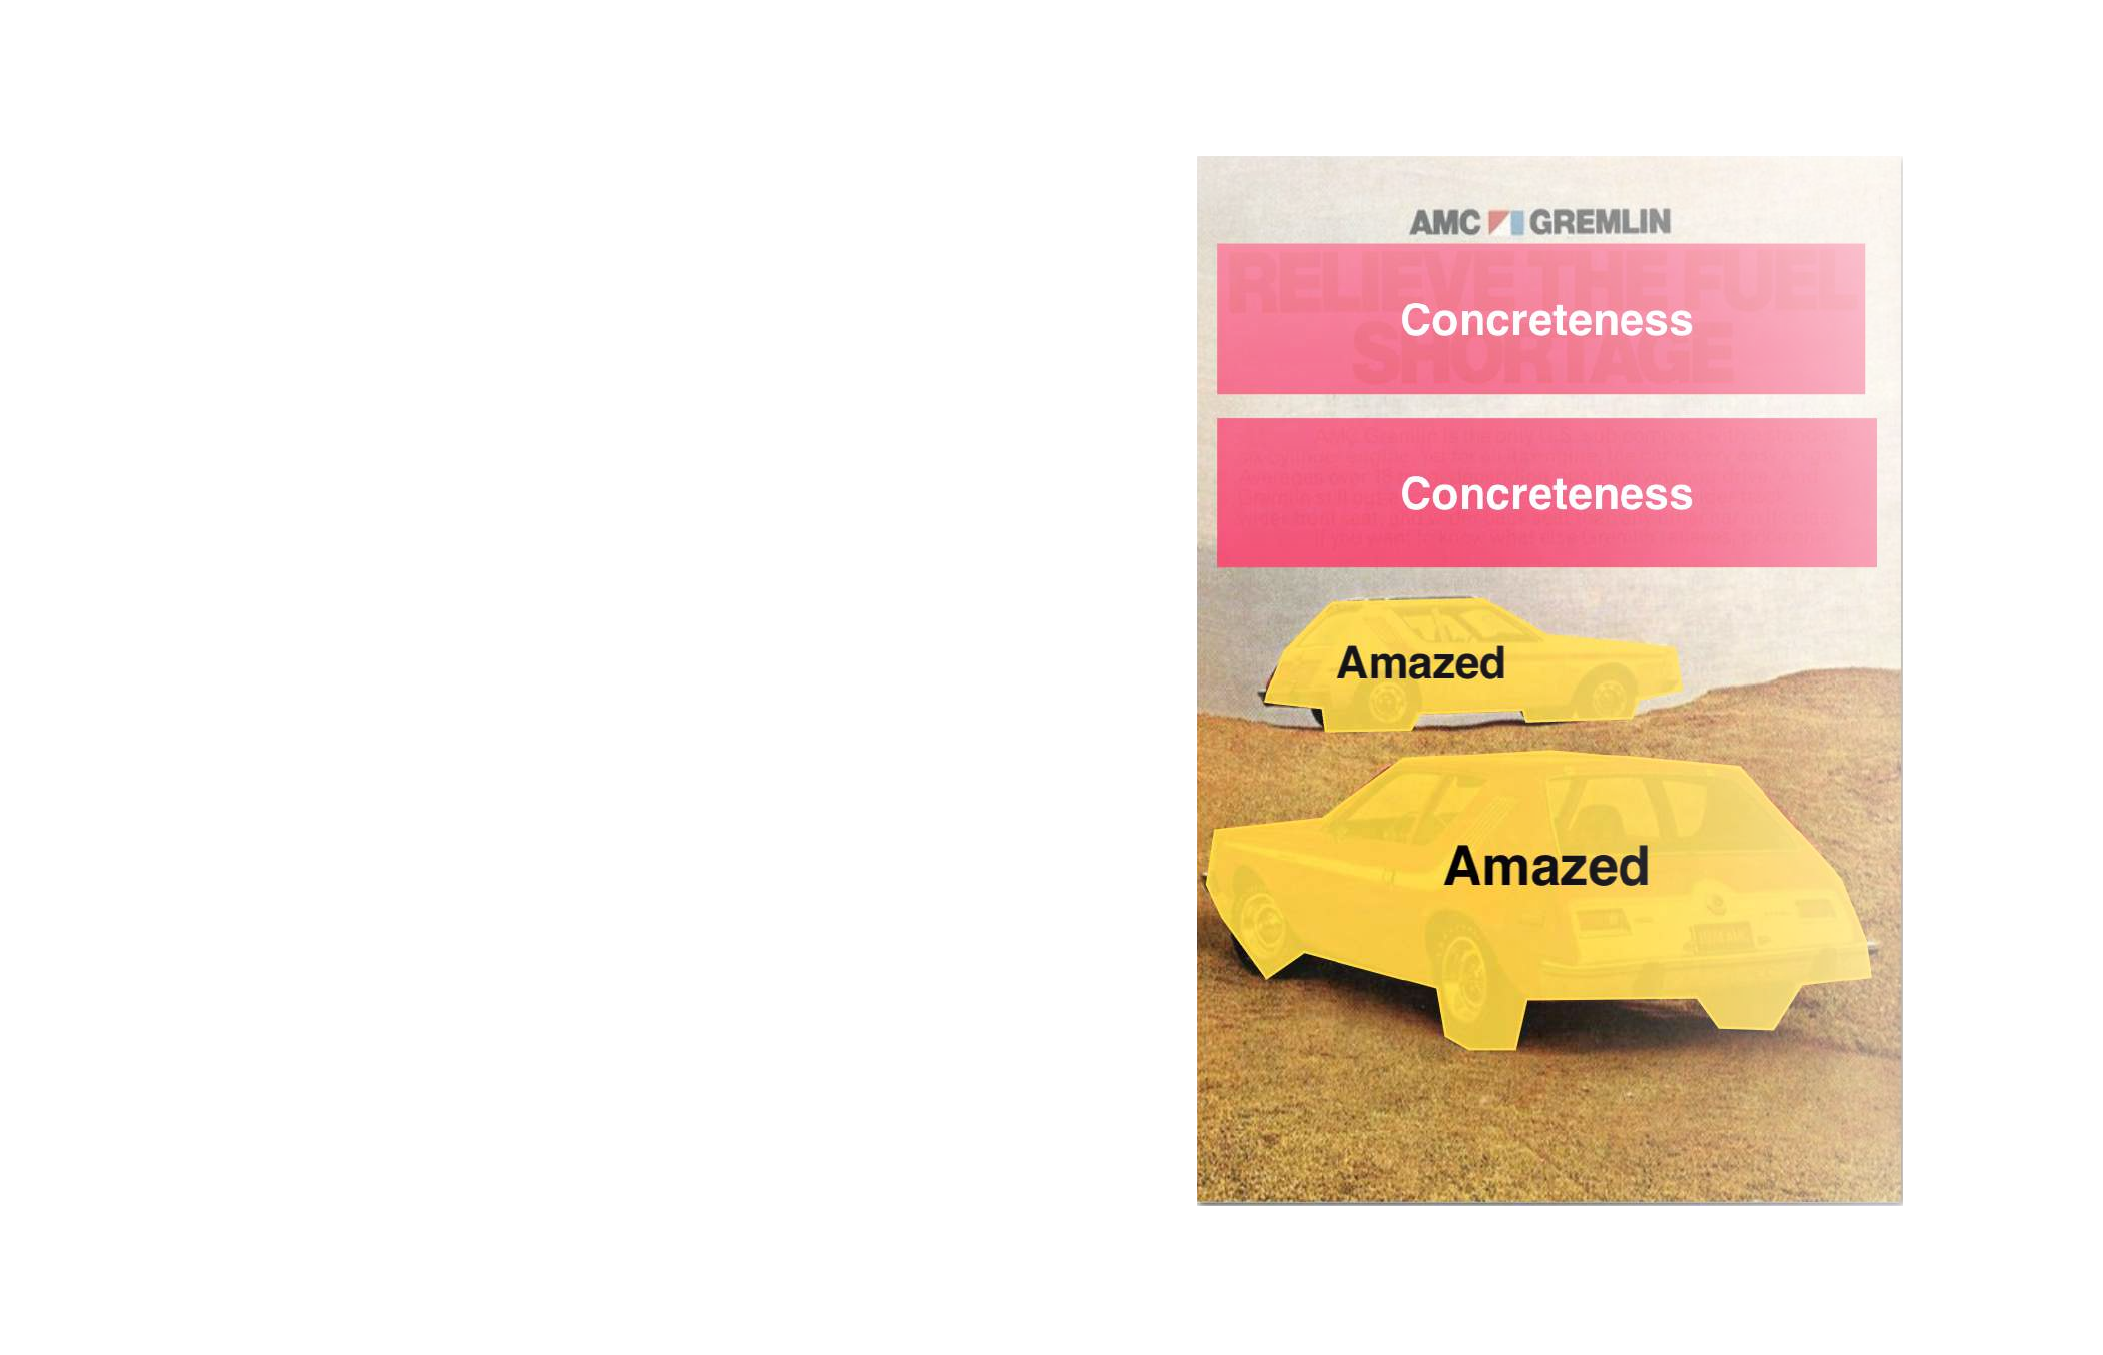
\includegraphics[scale=0.22]{images/fuel-shortage-segmented.pdf}
     \end{subfigure}
     \begin{subfigure}[b]{0.24\textwidth}
         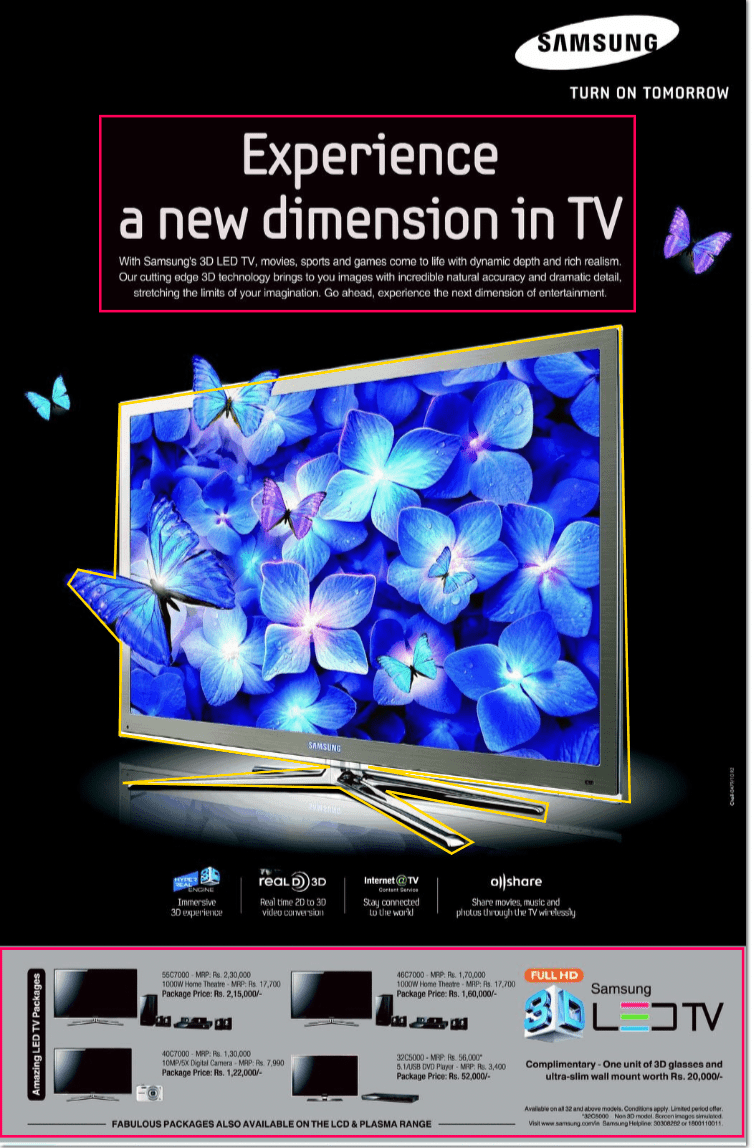
\includegraphics[scale=0.22]{images/Image2.png}
     \end{subfigure}
     \begin{subfigure}[b]{0.24\textwidth}
         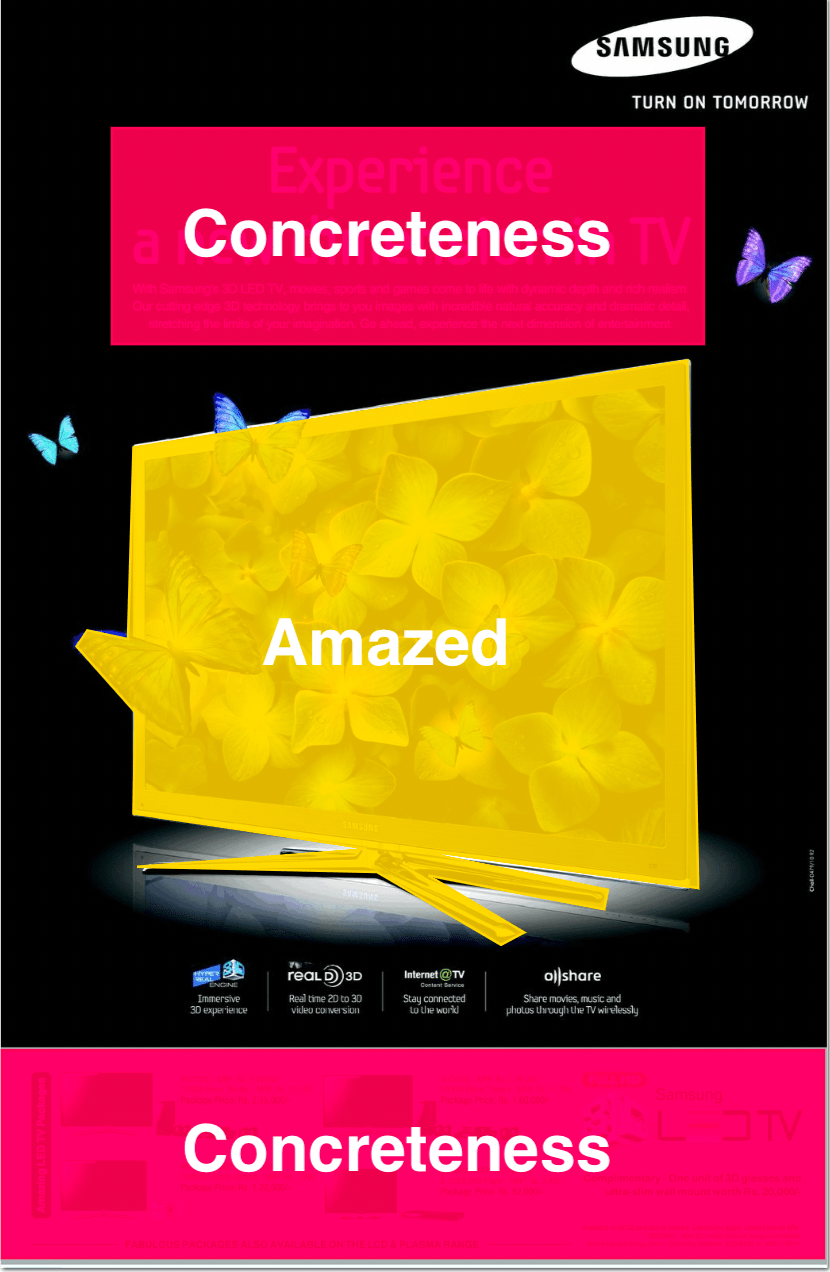
\includegraphics[scale=0.22]{images/Image2_Segment.png}
     \end{subfigure}


    \begin{subfigure}[b]{0.24\textwidth}
        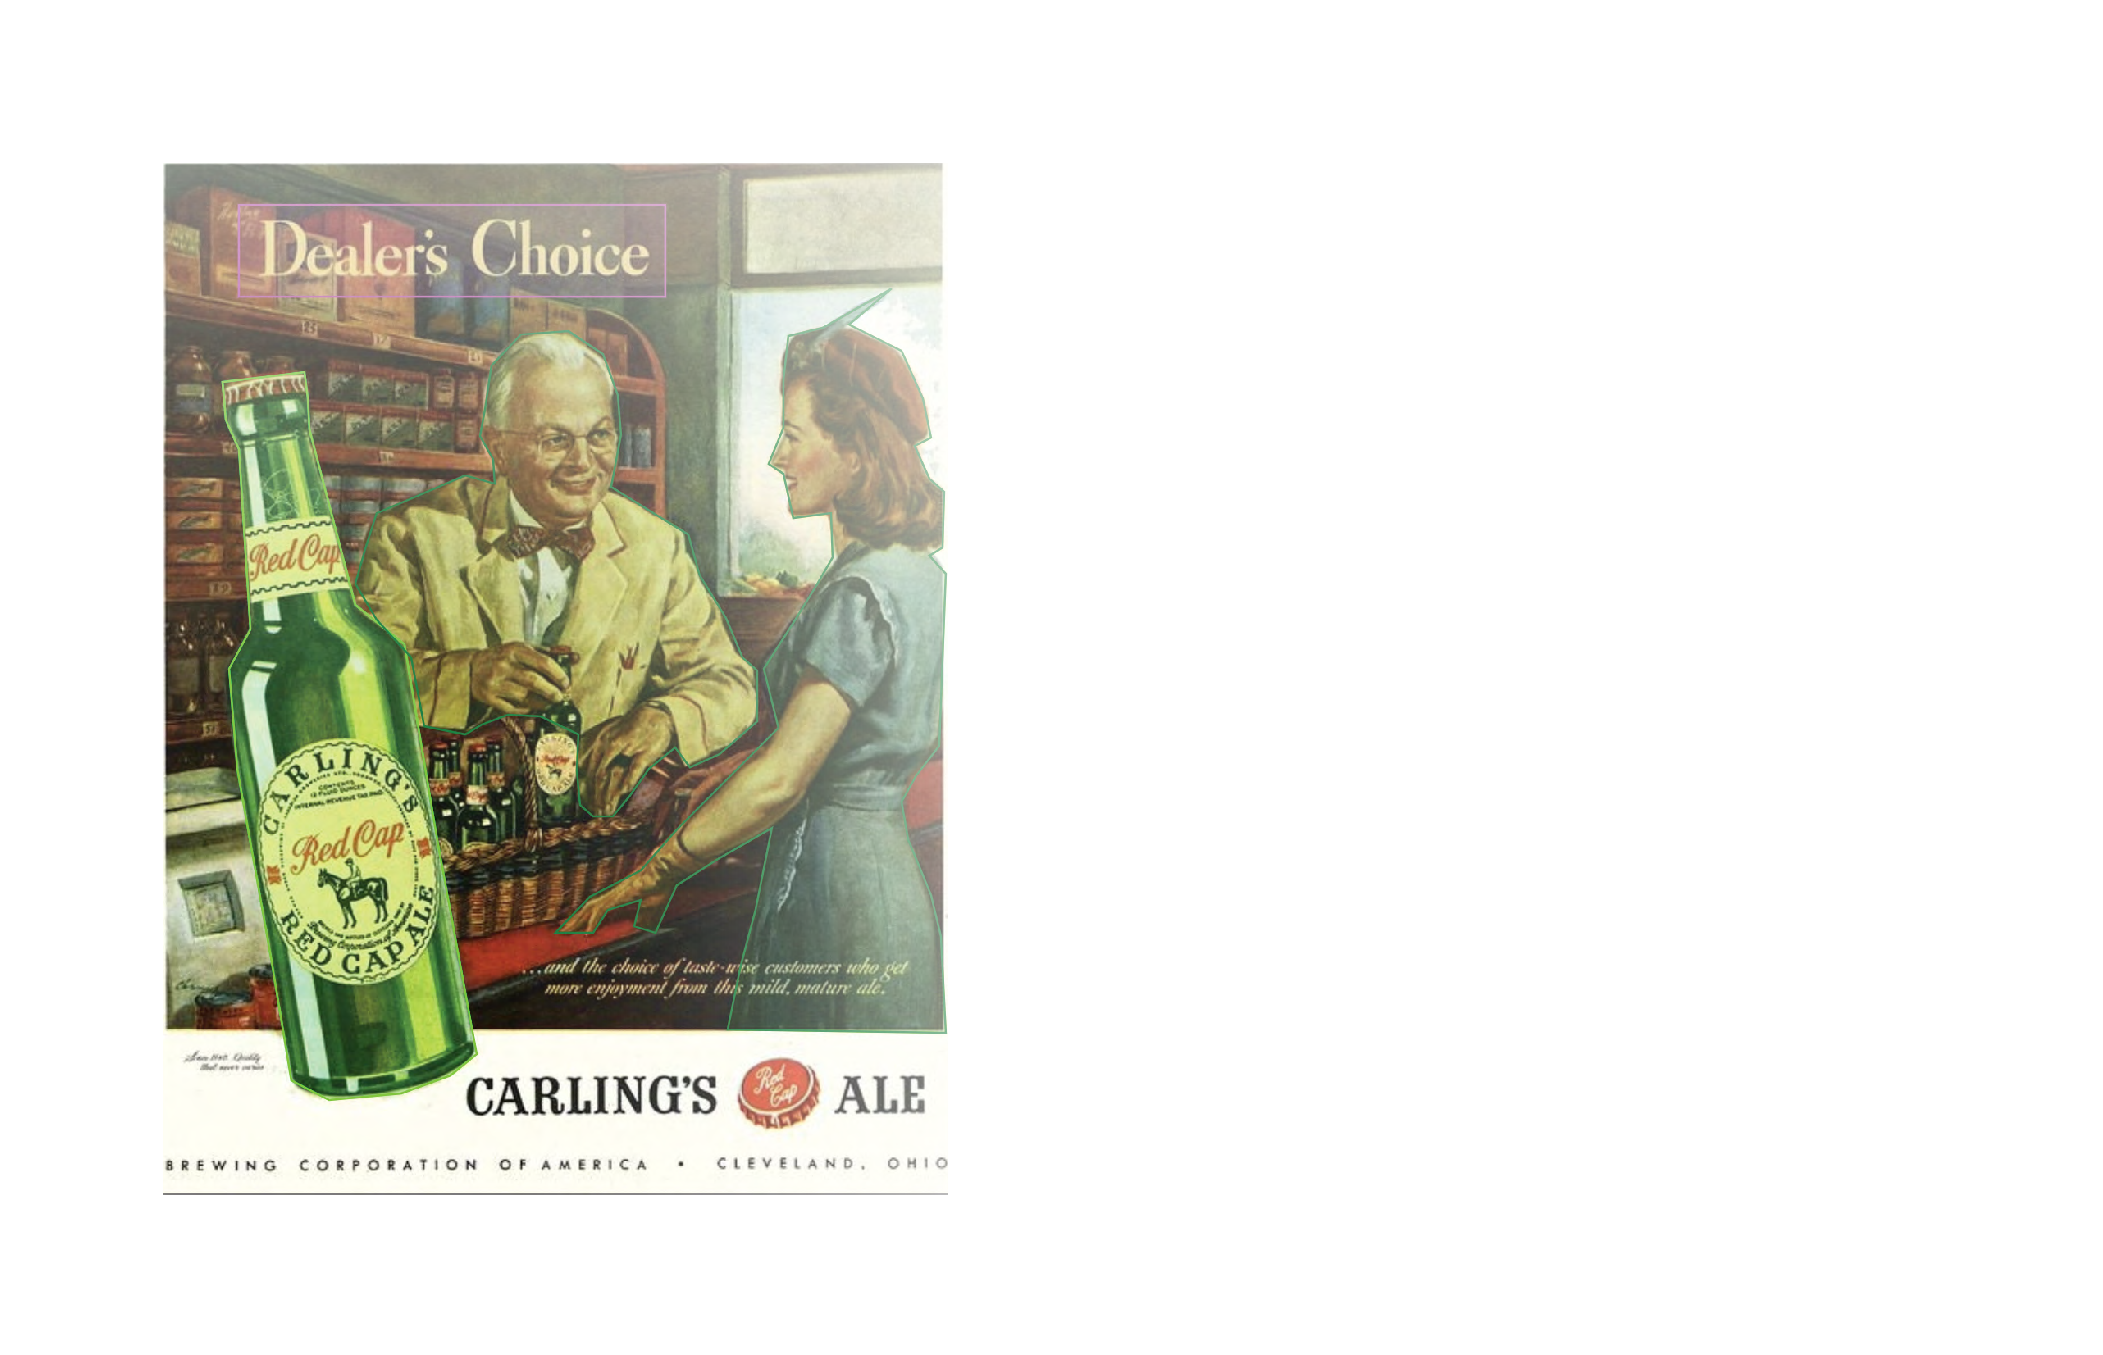
\includegraphics[scale=0.22]{images/dealer-choice-original.pdf}
    \end{subfigure}
    \begin{subfigure}[b]{0.24\textwidth}
        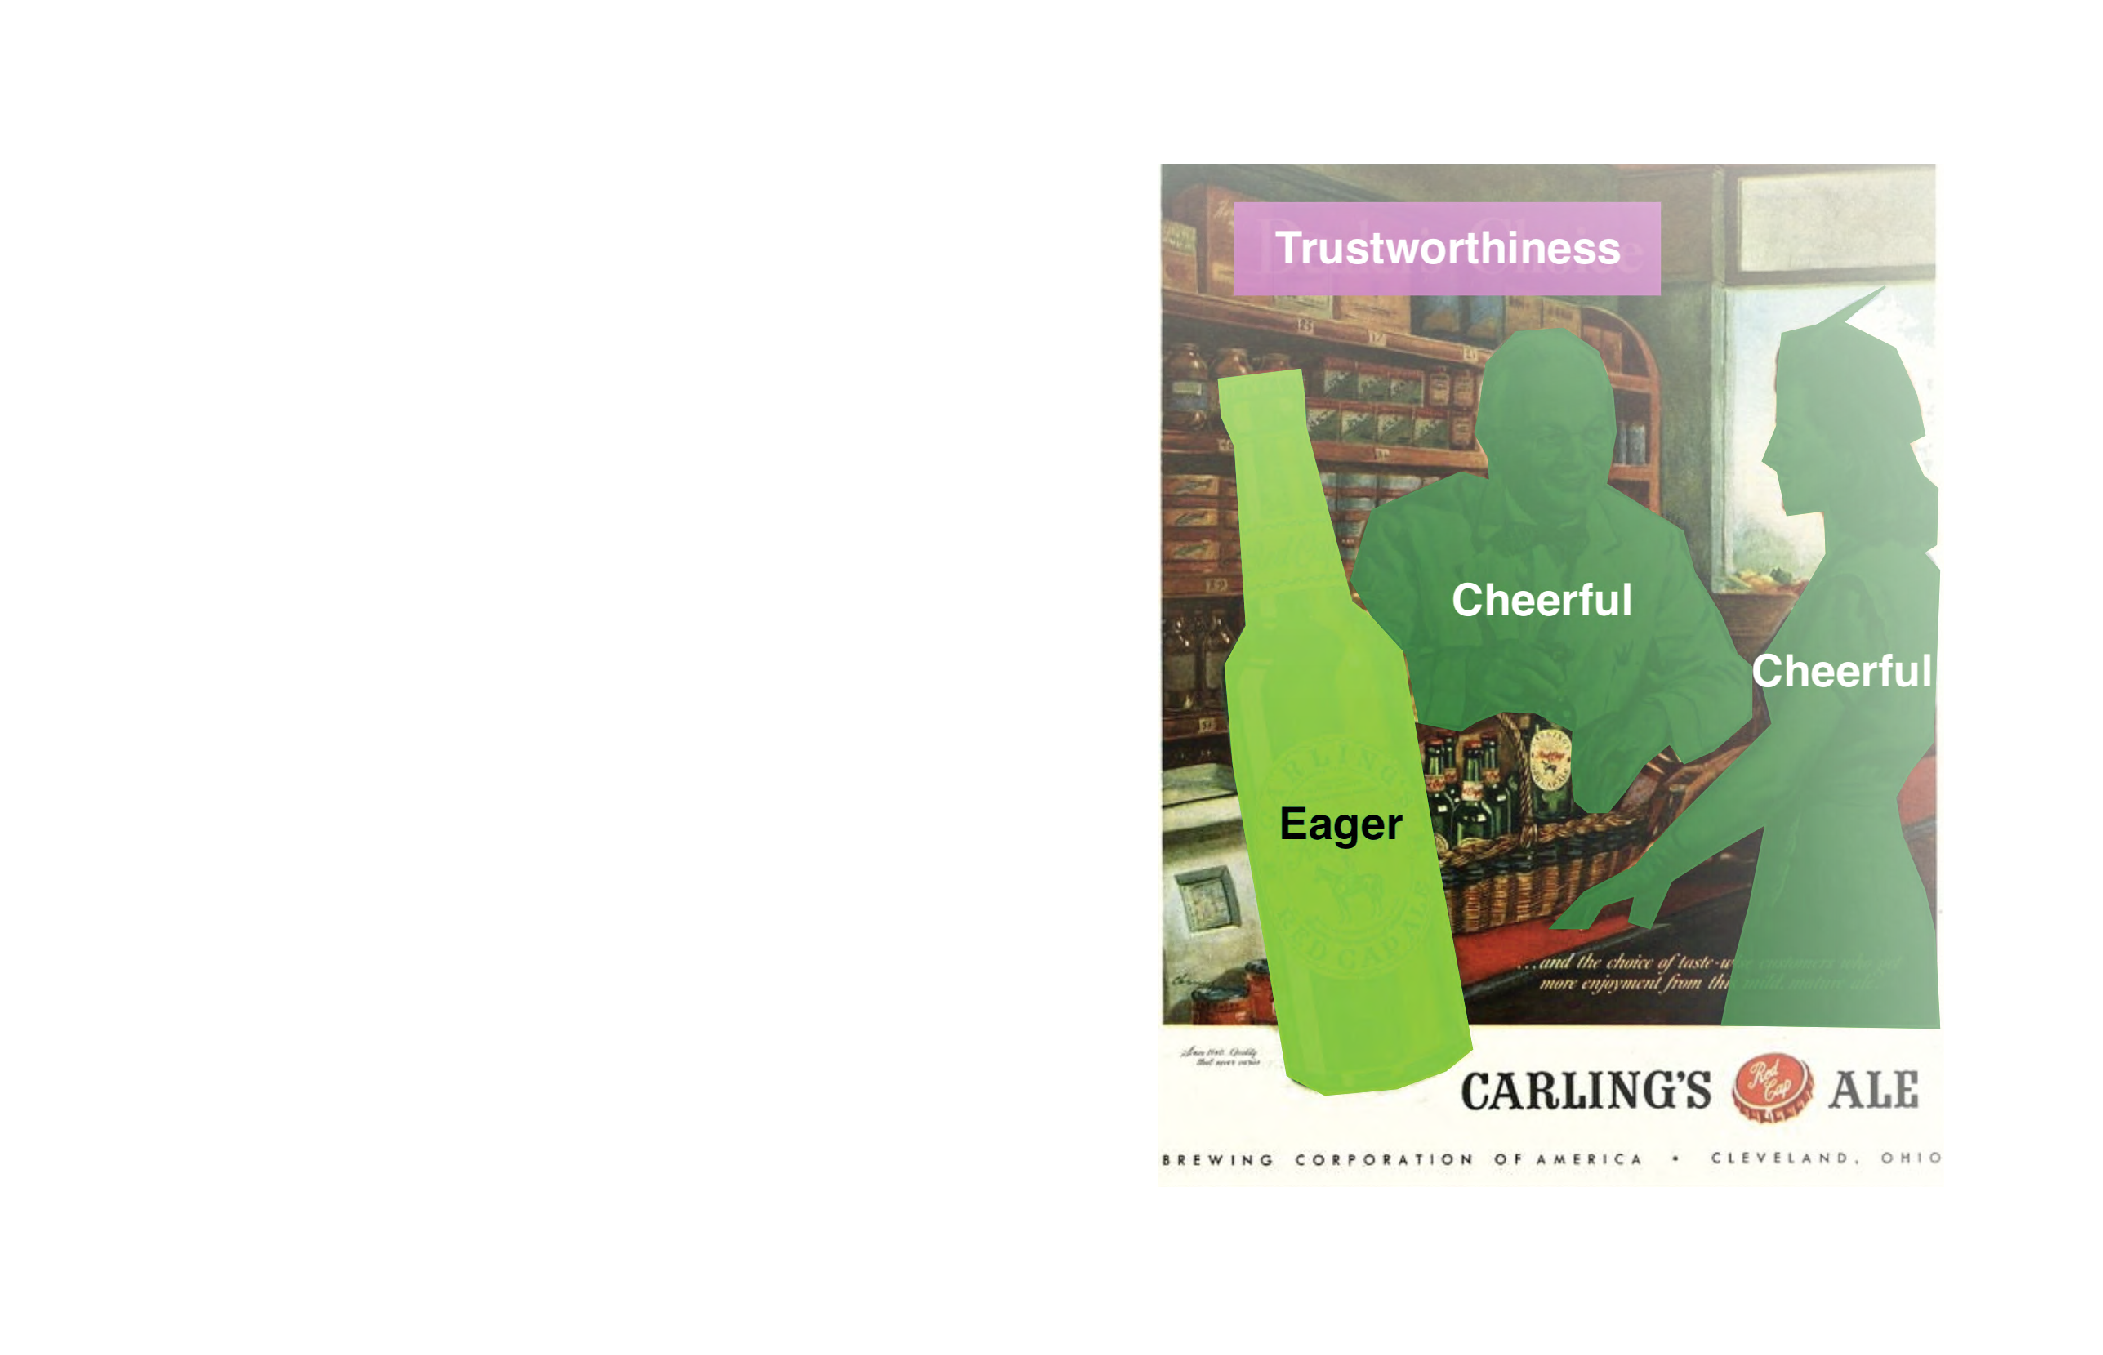
\includegraphics[scale=0.22]{images/dealer-choice-segmented.pdf}
    \end{subfigure}
     \begin{subfigure}[b]{0.24\textwidth}
         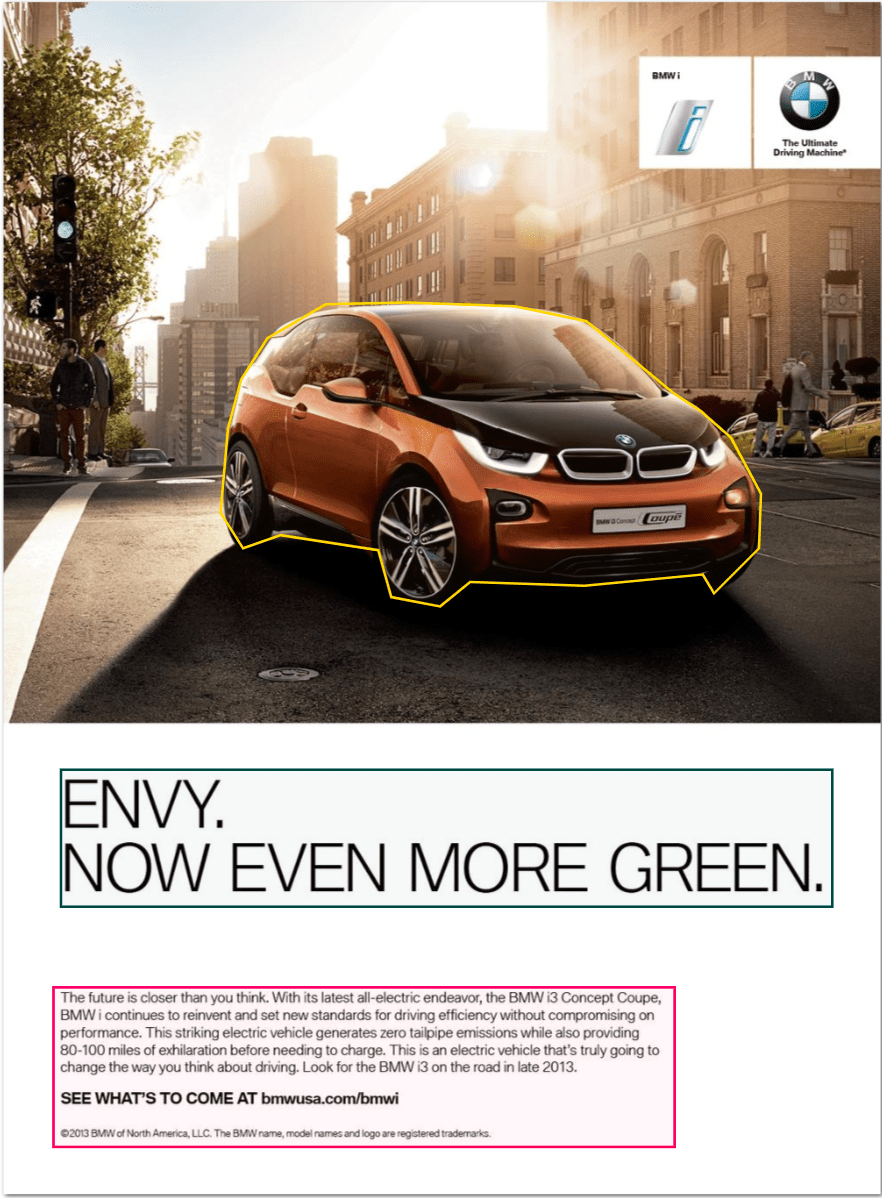
\includegraphics[scale=0.22]{images/Image3.png}
     \end{subfigure}
     \begin{subfigure}[b]{0.24\textwidth}
         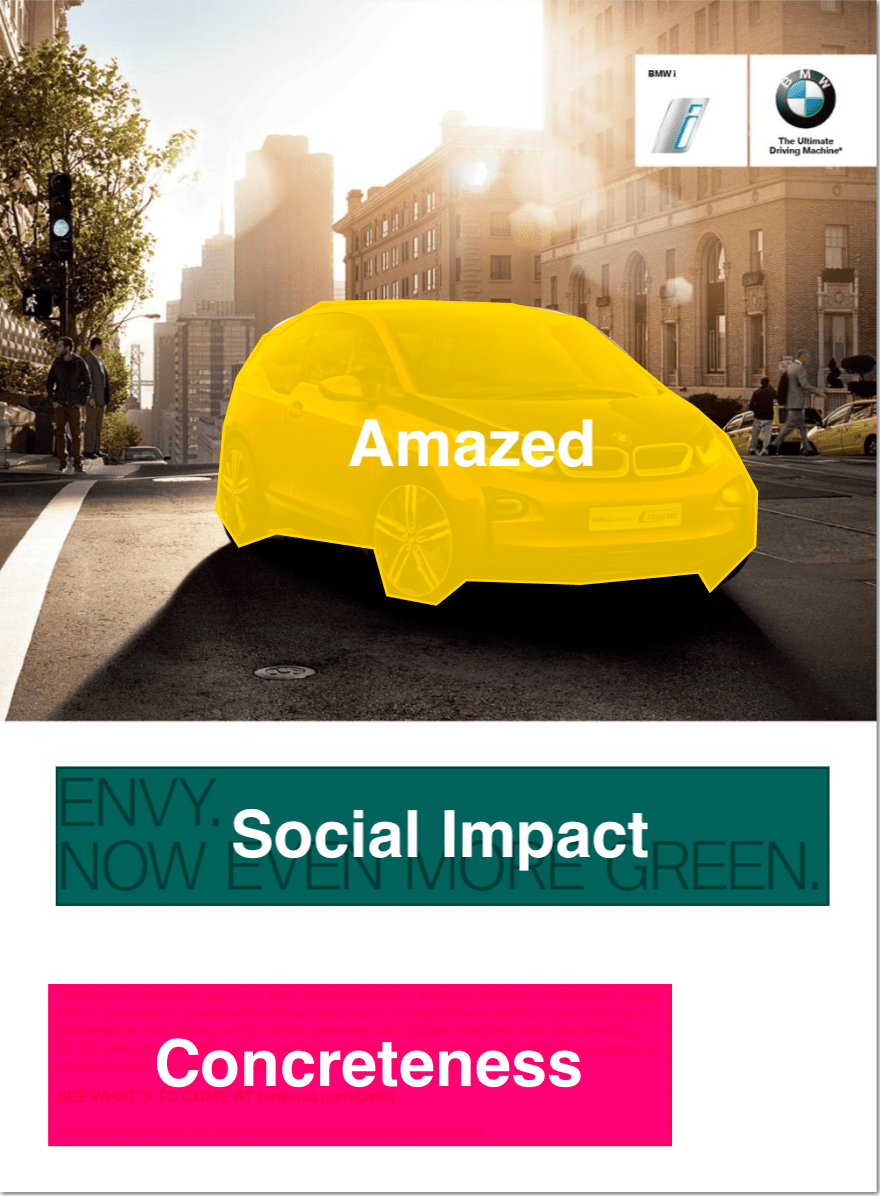
\includegraphics[scale=0.22]{images/Image3_Segment.png}
     \end{subfigure}
     
     \begin{subfigure}[b]{0.4\textwidth}
         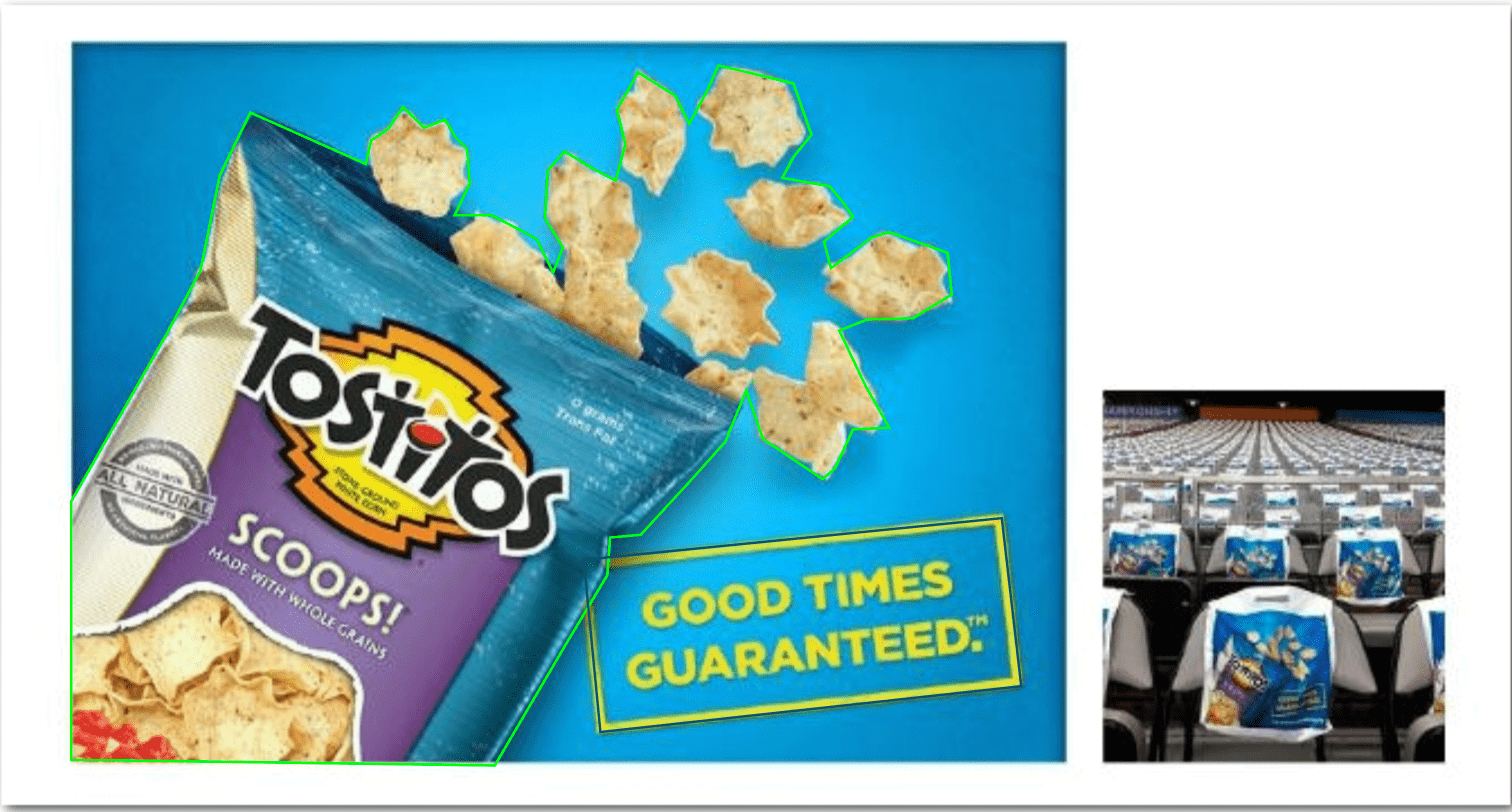
\includegraphics[scale=0.22]{images/Image4.png}
     \end{subfigure}
     \begin{subfigure}[b]{0.4\textwidth}
         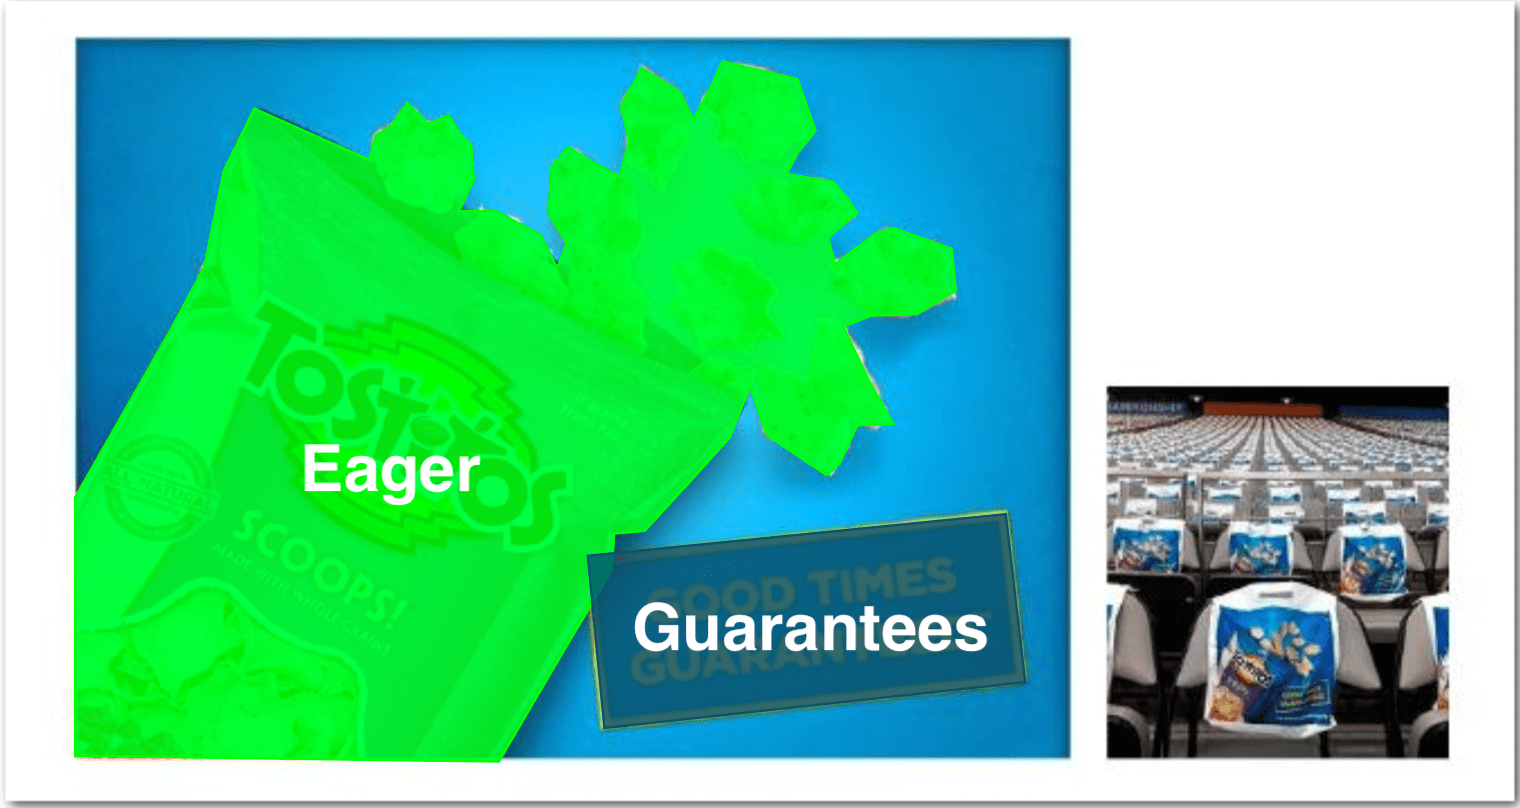
\includegraphics[scale=0.22]{images/Image4_Segment.png}
     \end{subfigure}
     
    \caption{\small \label{fig:segmented image} Image with a segmentation mask depicting the strategies \textit{Emotion:Cheerful}, \textit{Emotion:Eager} and \textit{Trustworthiness}.}
    % \vspace{-4mm}
\end{figure*}







Next, we calculate the Dice correlation coefficient\footnote{The Dice Coefficient is defined as: \; \(2*|X \cap Y|\: / \:(|X|+|Y|)\), where X and Y are two sets; a set with vertical bars on either side refers to the cardinality of the set, i.e. the number of elements in that set; and \(\cap\)  refers to the intersection of two sets.} statistics for pairs of co-occurring persuasion strategies. The top-5 pairs are eager-concreteness (0.27), scarcity-reciprocity (0.25), eager-cheerful (0.19), amazed-concreteness (0.17), and eager-reciprocity (0.17). We find that these correlation values are not particularly high since marketers seldom use \textit{common pairings} of messaging strategies to market their products. The visual part mostly shows eager strategy in ads; therefore, we find that the text modality becomes free to show other strategies. That is why primarily text-based concreteness, cheerfulness, and reciprocity strategies are present with the visual-based eager strategy in the text modality. Also, primarily vision-based amazement, eagerness, and scarcity (short-text) strategies co-occur with text-based reciprocity and concreteness (\textit{e.g.}, Fig.~\ref{fig:footwear-strategies}).


\begin{figure*}
    \centering
    \begin{subfigure}[b]{0.3\textwidth}
         \centering
         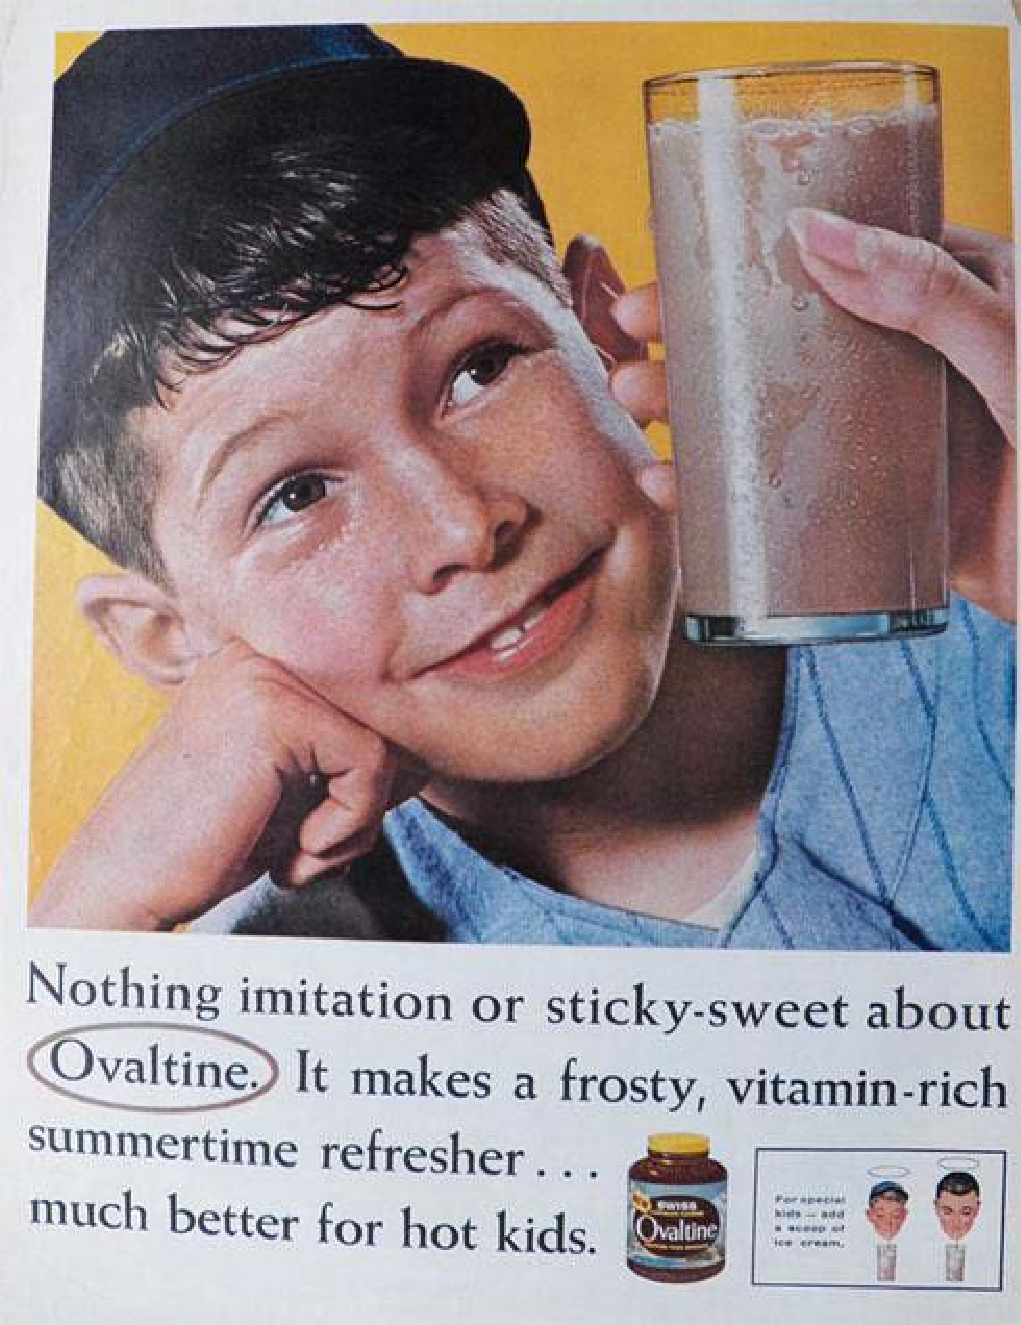
\includegraphics[width=\textwidth,scale=0.6]{images/humans_concreteness_img1.pdf}
         \caption{}
         
     \end{subfigure}
     \begin{subfigure}[b]{0.3\textwidth}
         \centering
         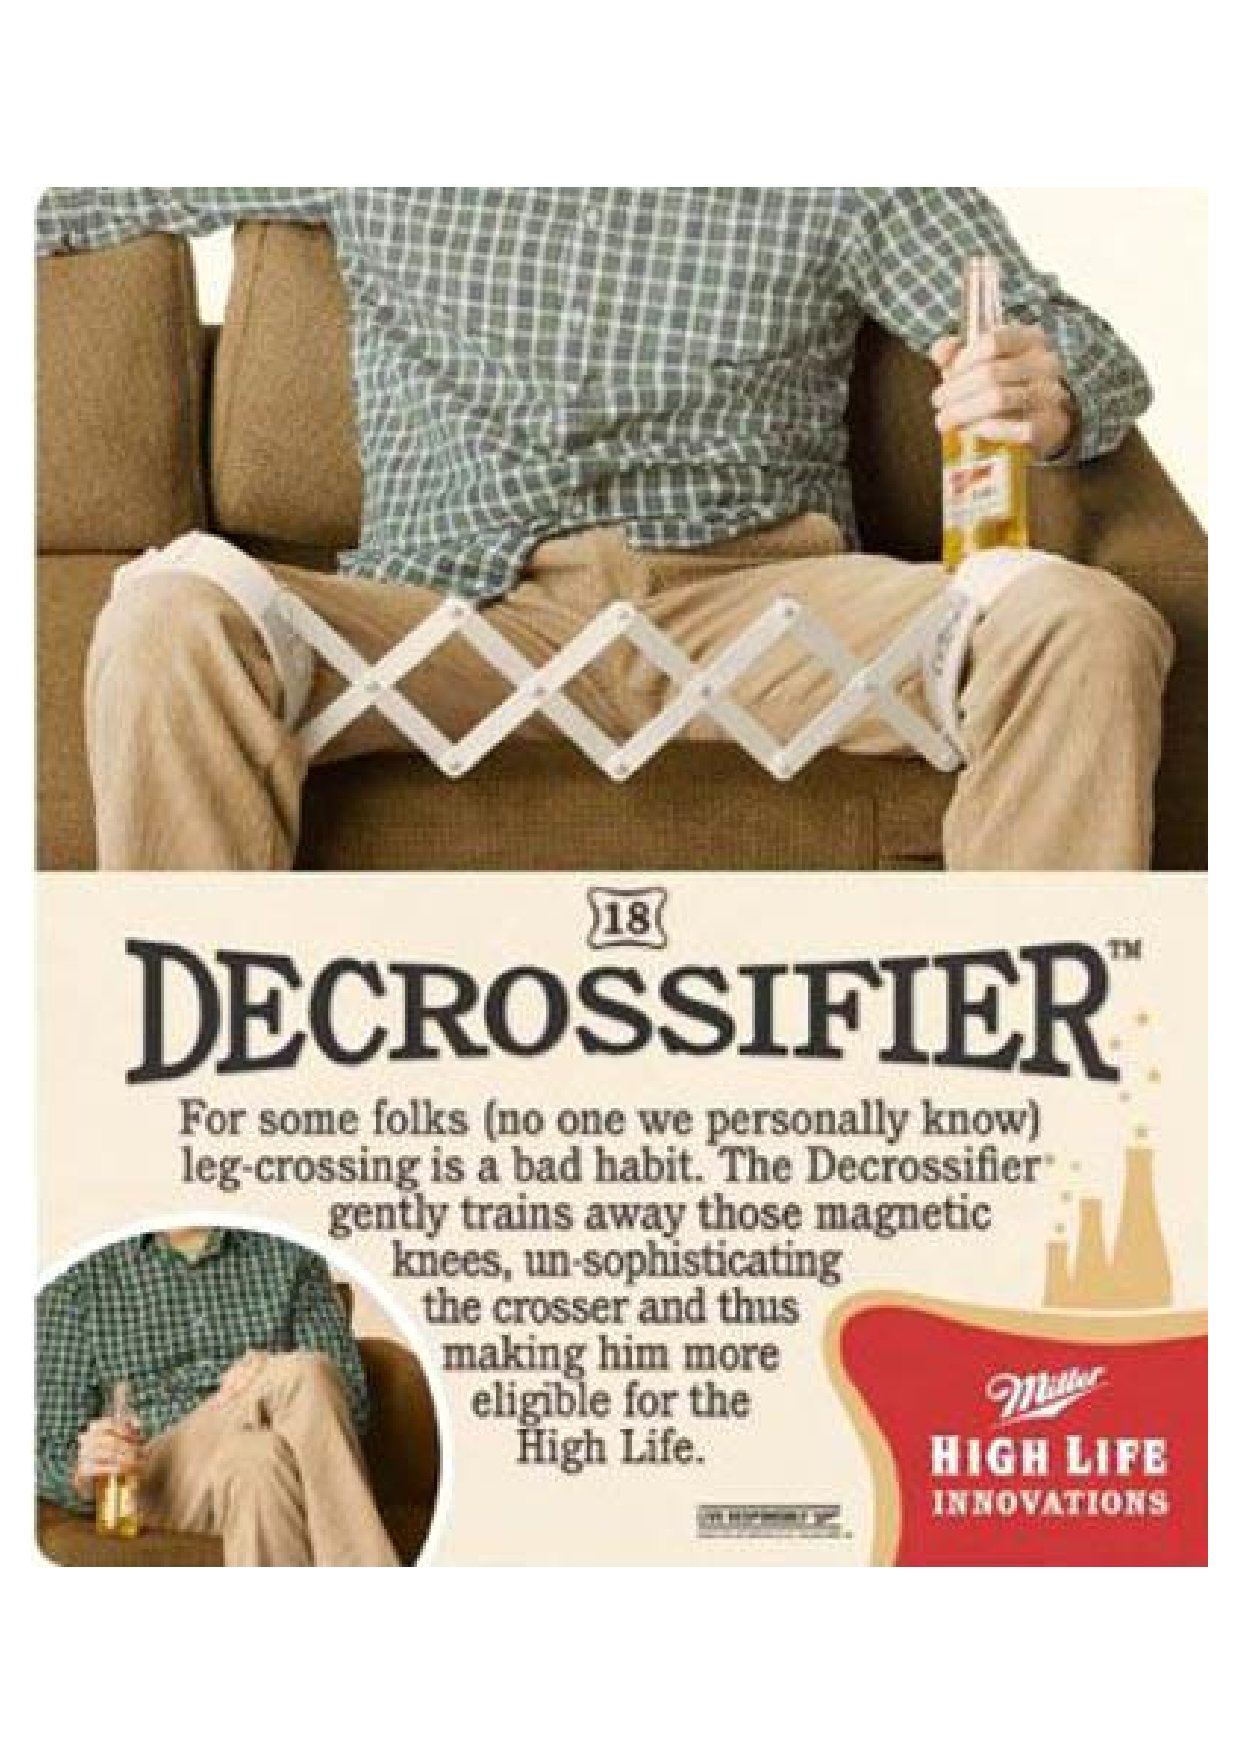
\includegraphics[width=\textwidth,scale=0.5]{images/humans_concreteness_img2.pdf}
         \caption{}
         
     \end{subfigure}
     \begin{subfigure}[b]{0.3\textwidth}
         \centering
         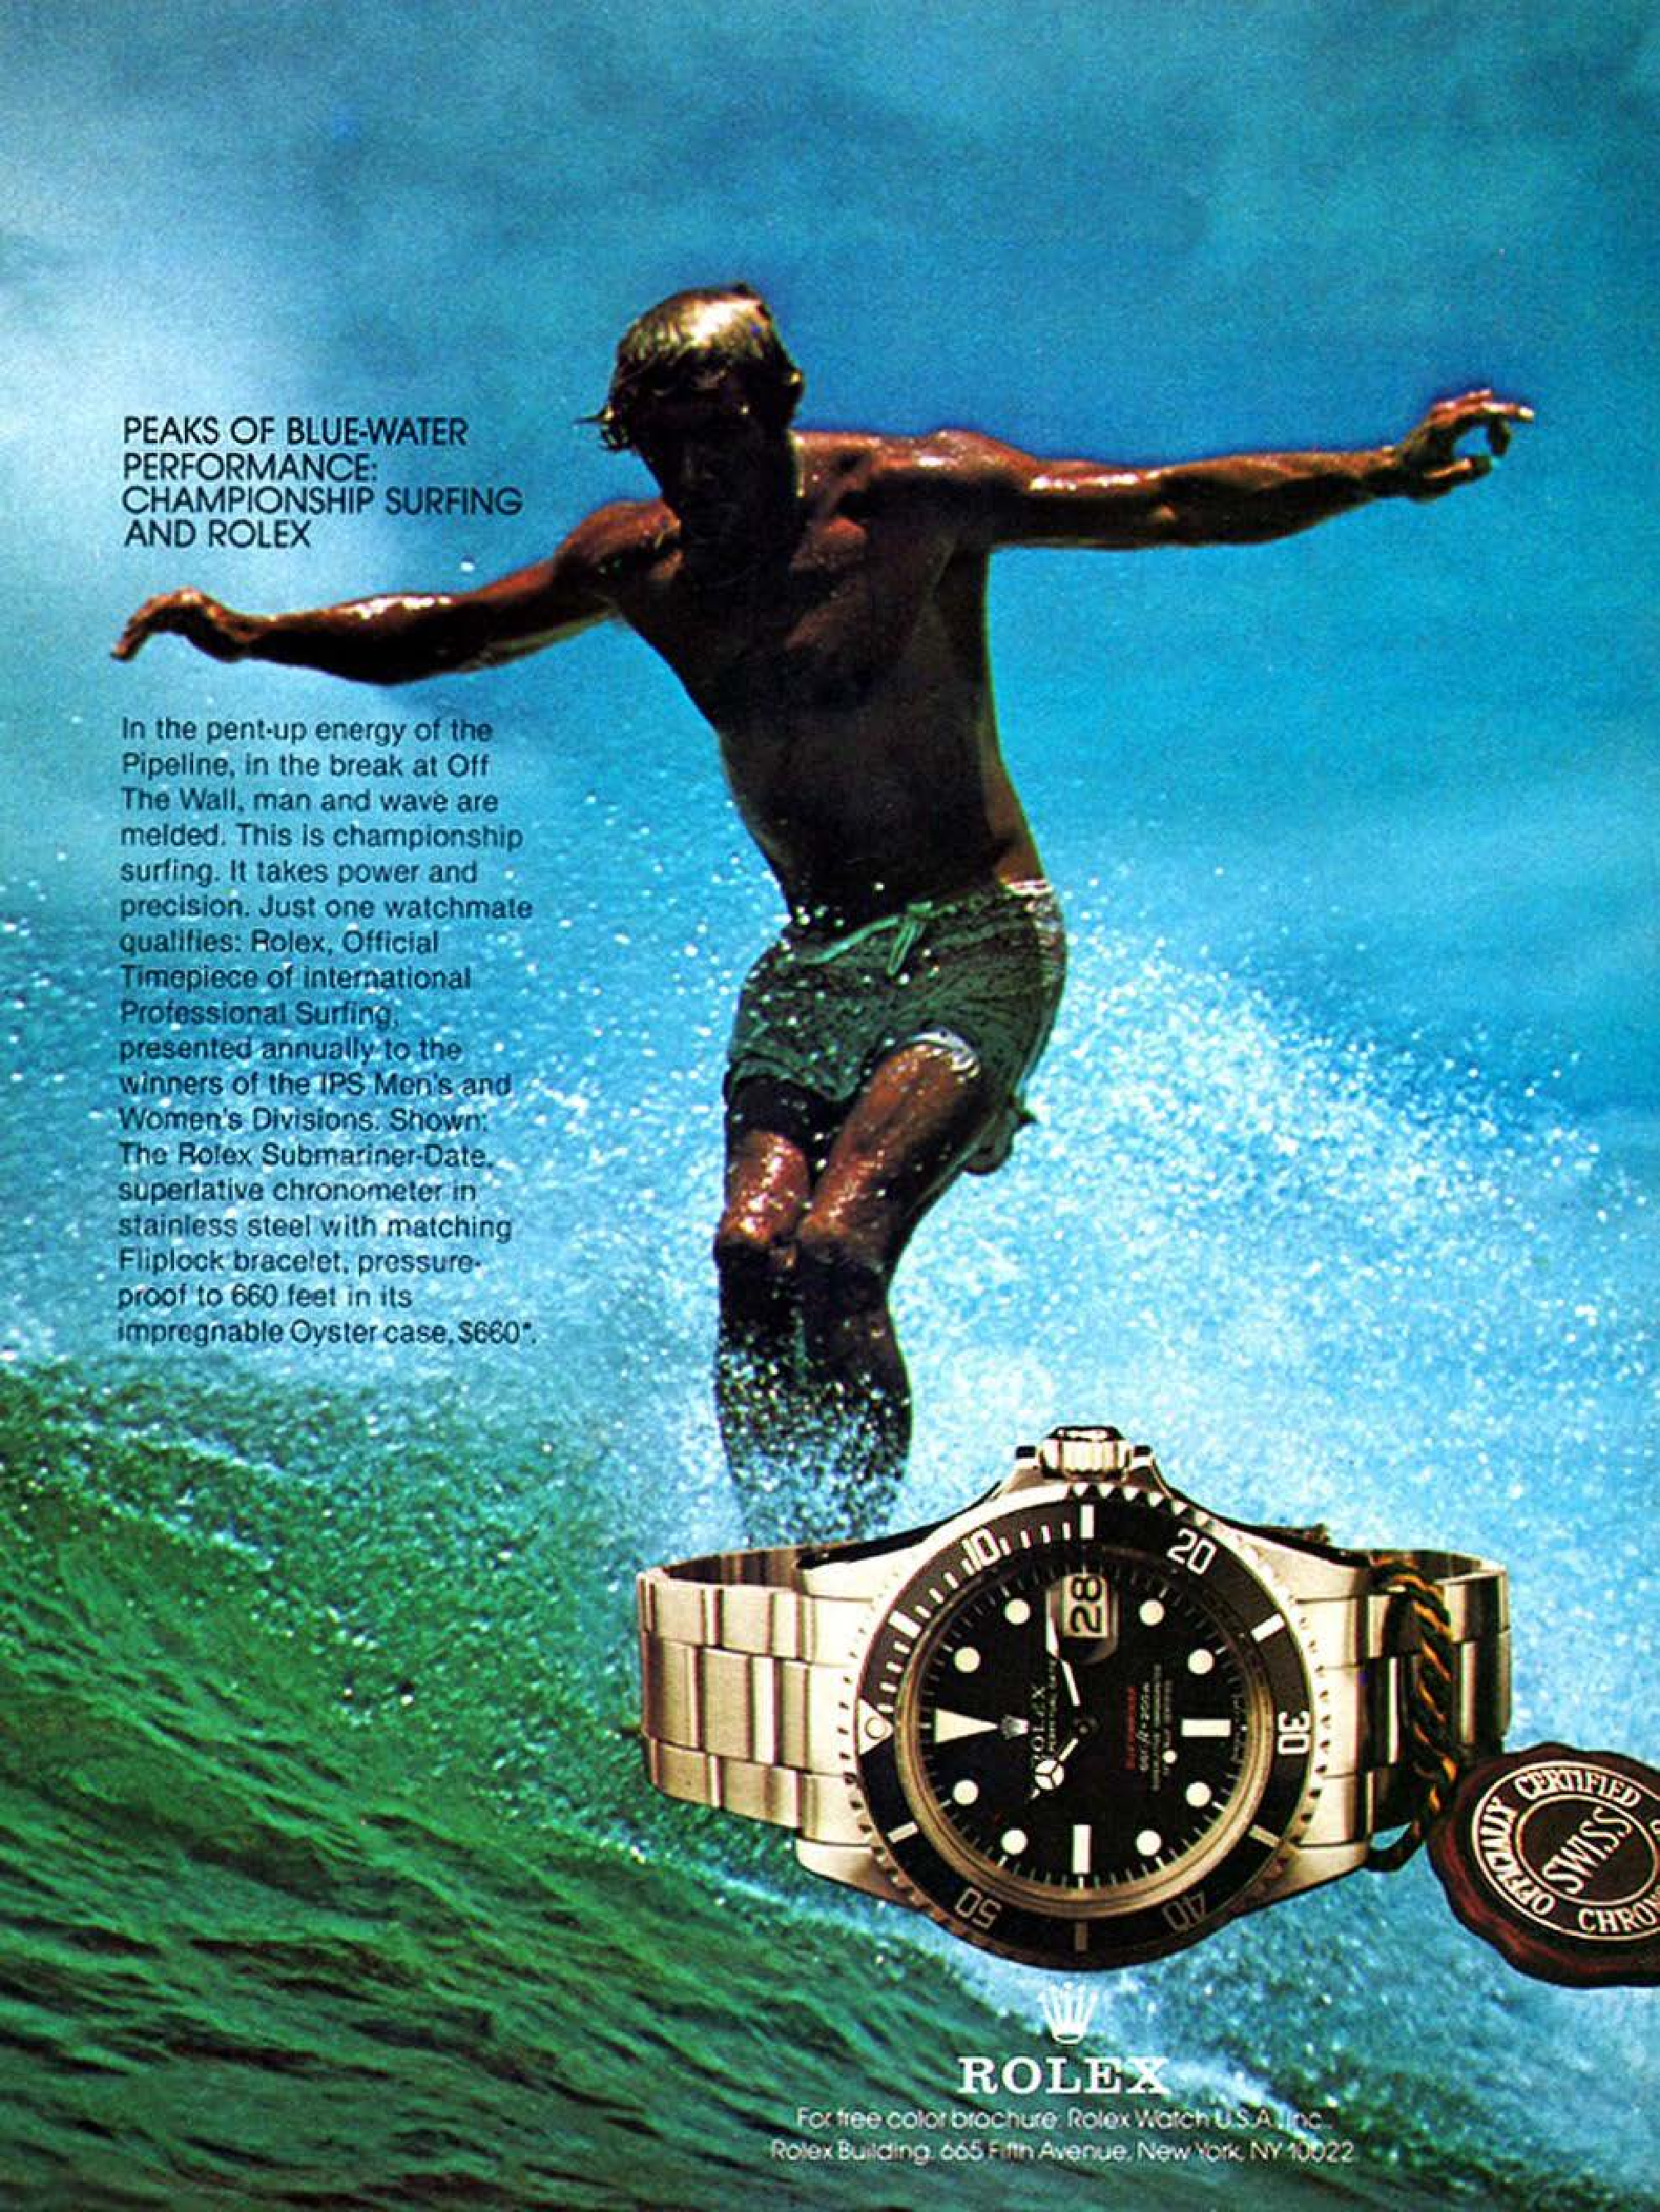
\includegraphics[width=\textwidth,scale=1.0]{images/humans_concreteness_img3.pdf}
         \caption{}
         
     \end{subfigure}
    \caption{Advertisements containing humans and concreteness}
    \label{fig:humans_concreteness-ads}
\end{figure*}




\begin{figure}[h]
        \centering
        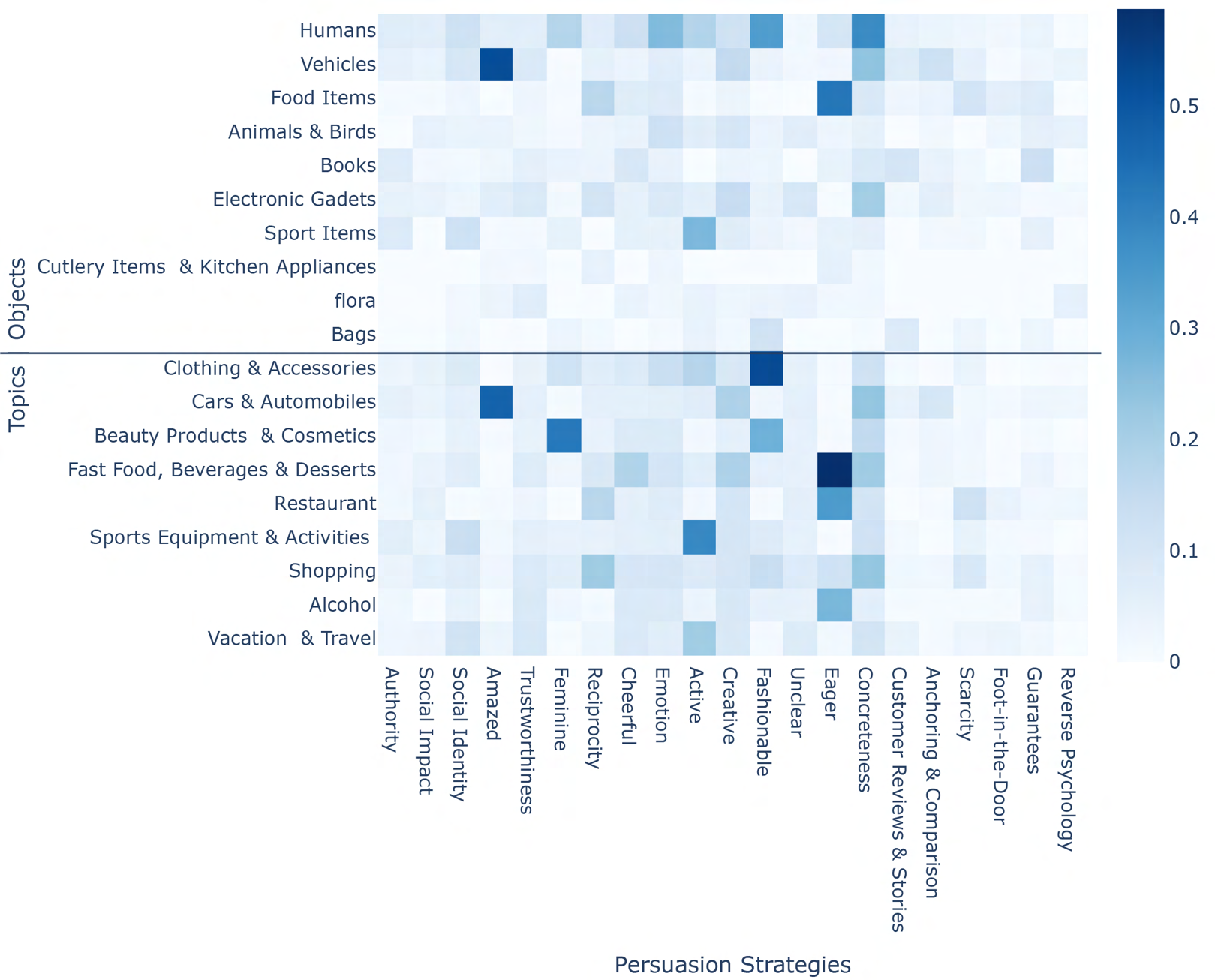
\includegraphics[scale=0.55]{images/objects_topics.pdf}
        \caption{Dice correlation between topics and strategies. Topics are taken from the Pitts Ad dataset and further similar topics are combined to get these values.}
        \label{fig:correlation-between-topics-and-strategies}
        % \vspace*{-3mm}
    \end{figure}

Next, we calculate the correlation between image topics and objects present with persuasion strategies. We see that the emotion:feminine and emotion:fashionable strategies are most often associated with beauty products and cosmetics (corr=0.4256, 0.2891). This is understandable since most beauty products are aimed at women. We see that the fast-food and restaurant industries often use eagerness as their messaging strategy (corr = 0.5877,0.3470). We find that the presence of humans in ads is correlated with the concreteness strategy (see Fig~\ref{fig:humans_concreteness-ads} for a few examples) (corr=0.3831). On the other hand, vehicle ads use emotion:amazed and concreteness (corr=0.5211,0.2412) (see Fig:\ref{fig:correlation-between-topics-and-strategies} for detailed correlations). 

Similar to a low correlation in co-occurring strategies, we find that product segments and their strategies are not highly correlated. This is because marketers use different strategies to market their products even within a product segment. Fig.~\ref{fig:footwear-strategies} shows an example in which the footwear industry (which is a subsegment of the apparel industry) uses different strategies to market its products. Further, for a batch of $250$ images, we also label segmented image regions corresponding to the strategies present in the image. These segment masks were also double-annotated. Fig.~\ref{fig:segmented image} presents an example of masks depicting parts of the image masked with different persuasion strategies in a drink advertisement.





\subsubsection{Persuasion Strategy Dataset For Video Advertisements}
For this task, we collected 2203 video advertisements from popular brands publicly available on the web. We use the following 12 strategies as our target persuasion strategy set: \textit{Social Identity, Concreteness, Anchoring and Comparison, Overcoming Reactance, Reciprocity, Foot-in-the-Door, Authority, Social Impact, Anthropomorphism, Scarcity, Social Proof,} and \textit{Unclear}. We use non-experts human annotators to label this dataset (as compared to expert humans for the image ads dataset). In order to make the class labels easier to understand for non-expert human annotators, we make a list of 15 yes/no type-questions containing questions like ``\textit{Was there any expert (person or company) (not celebrity) encouraging to use the product/brand? Was the company showcasing any awards (e.g., industrial or government)? Did the video show any customer reviews or testimonials?}'' (complete list in Table~\ref{table:persuasion strategy questions}). 

Each human annotator watches 15 videos such that each video gets viewed by at least two annotators and answers these questions for each video. Based on all the responses for a video, we assign labels to that video. We remove videos with an inter-annotator score of less than 60\%. After removing those, we get a dataset with 1002 videos, with an average length of 33 secs and a distribution as shown in Fig.~\ref{fig:persuasion-strategy-dataset-distribution}. This dataset is then used for the persuasion strategy identification task. 


\begin{figure}[!h]
    \centering
    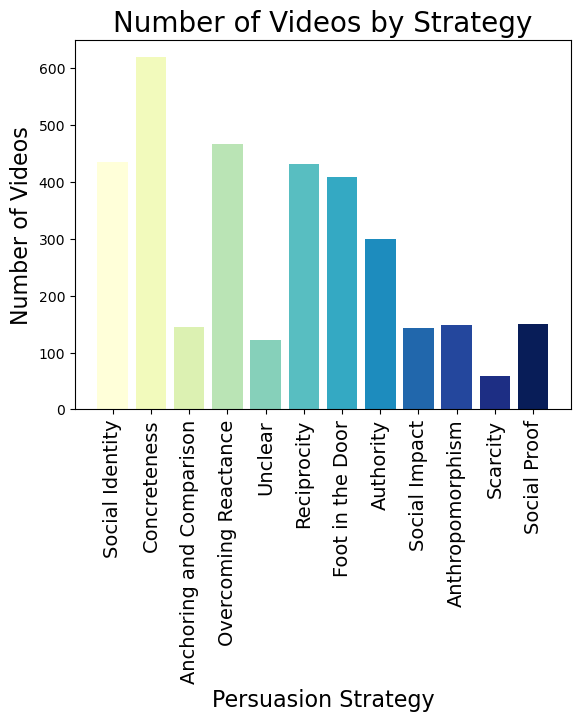
\includegraphics[width=0.5\textwidth]{images/video_strategies.png}
    \caption{Distribution of persuasion strategies in our video persuasion strategy dataset}
    \label{fig:persuasion-strategy-dataset-distribution}
\end{figure}


\begin{table*}[!hp]
  \centering
  \begin{tabular}{|p{3.5cm}|p{2.3cm}|p{3.5cm}|p{2.3cm}|}
    \hline
    \textbf{Question} & \textbf{Strategy} & \textbf{Question} & \textbf{Strategy} \\
    \hline
    Was there any expert (person or company) (not celebrity) encouraging to use the product/brand? & Authority & Did the video show any normal customers (non-expert, non-celebrity) using the product? & Social Identity \\
    \hline
    Did the video showcase any awards or long usage history of the product/brand? & Authority & Did the video show any customer reviews or testimonials? & Social Proof \\
    \hline
    Was the product/brand comparing itself with other competitors or existing solutions? & Anchoring and Comparison & Were any number/statistics mentioned? & Concreteness \\
    \hline
    Did the video talk about any specific features or provide information about the product/brand? & Concreteness & Were there any mention of any offers on the brand/product? & Reciprocity \\
    \hline
    Were the offers limited or available for a short period of time? & Scarcity & Was the product/brand told to be free or available on a discount? & Foot in the Door, Reciprocity \\
    \hline
    Was the brand/product described as simple, easy to use, or can start using with minimal resistance? & Overcoming Reactance, Foot in the Door & Was the brand/product talking about bigger societal impact? & Social Impact \\
    \hline
    Did the brand provide any guarantees that might help reduce the risk of people trying out the product? & Overcoming Reactance & Did the video provide any resources, tips, guides, or tools related to the product? & Reciprocity \\
    \hline
    Is the brand or product portrayed as human-like? & \makecell{Anthropo-\\morphism} & & \\
    \hline
  \end{tabular}
  \caption{The questions we asked to the non-expert annotators to help them identify persuasion strategy contained in the video advertisement. \label{table:persuasion strategy questions}}
\end{table*}





% \vspace{-2mm}
\subsection{Modeling: Persuasion Strategy Prediction}
\label{sec:Persuasion Strategy Prediction Model}


\begin{figure}[!h]
    \centering
    \begin{subfigure}[b]{0.49\textwidth}
         \centering
         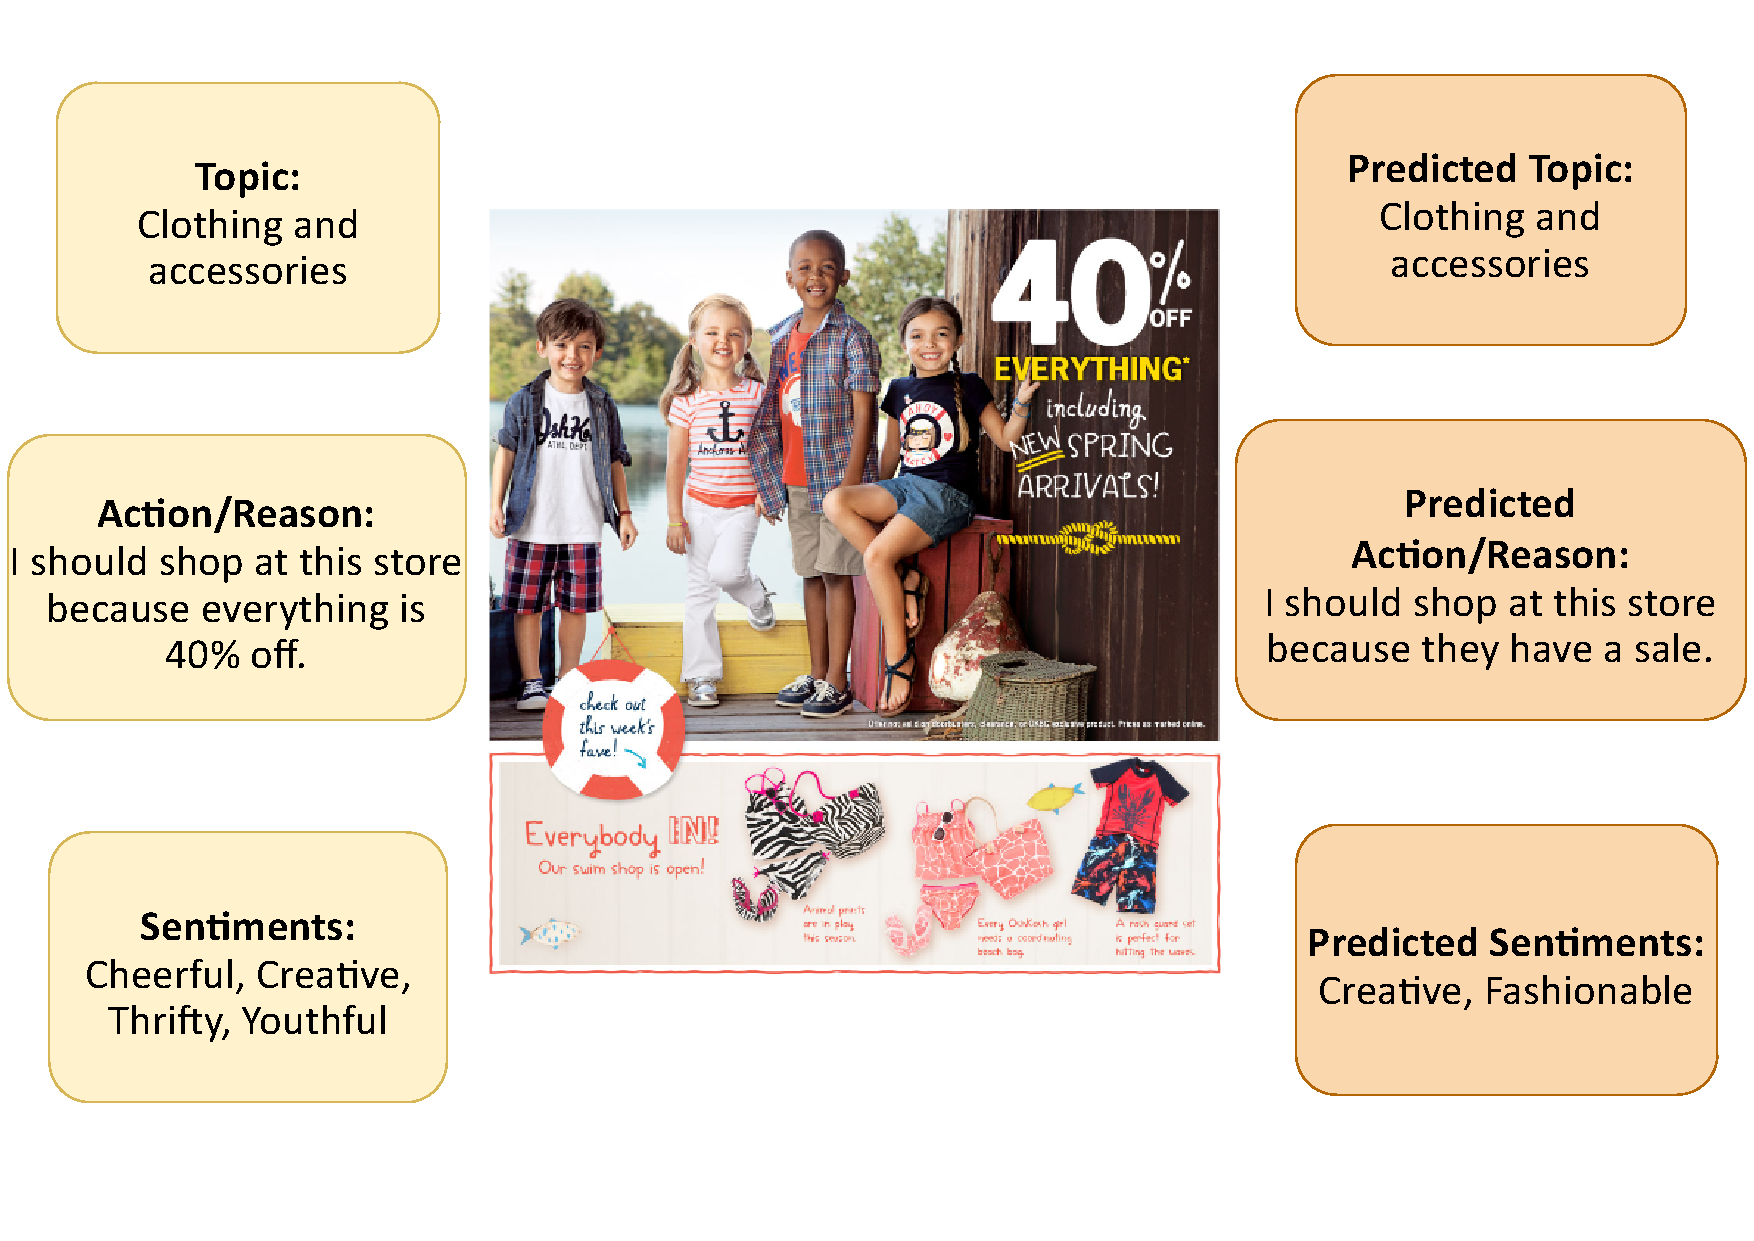
\includegraphics[width=\textwidth,scale=0.68]{images/preds_sup_1.pdf}
         \caption{}
         \label{fig:preds-sup-1}
        %  \vspace{-3pt}
     \end{subfigure}
     \begin{subfigure}[b]{0.49\textwidth}
         \centering
         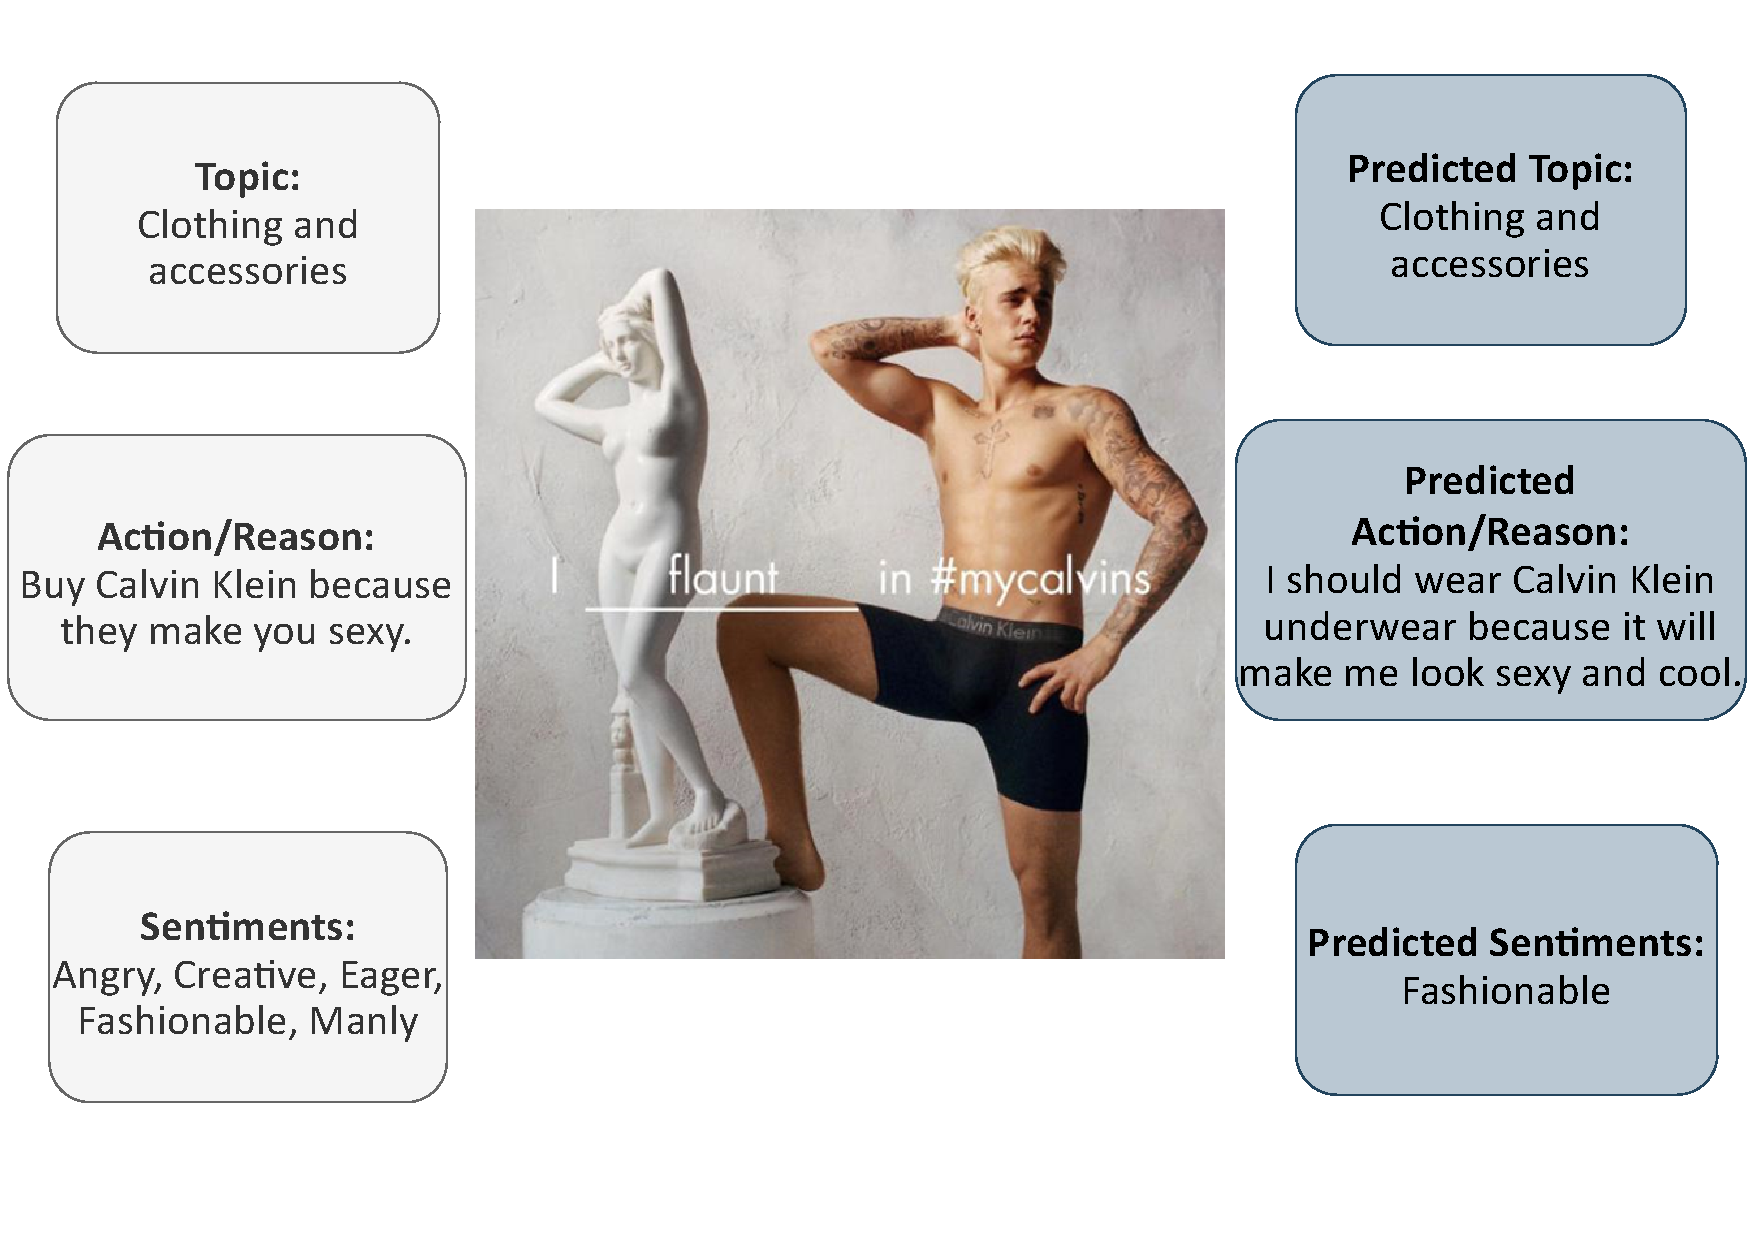
\includegraphics[width=\textwidth,scale=0.68]{images/preds_sup_2.pdf}
         \caption{}
         \label{fig:preds-sup-2}
        %  \vspace{-3pt}
     \end{subfigure}
    %  \begin{subfigure}[b]{0.49\textwidth}
    %      \centering
    %      \includegraphics[width=0.8\textwidth,scale=0.68]{LaTeX/images/preds_sup_5.pdf}
    %      \caption{}
    %      \label{fig:preds-sup-5}
    %      \vspace{-10pt}
    %  \end{subfigure}
     \begin{subfigure}[b]{0.49\textwidth}
         \centering
         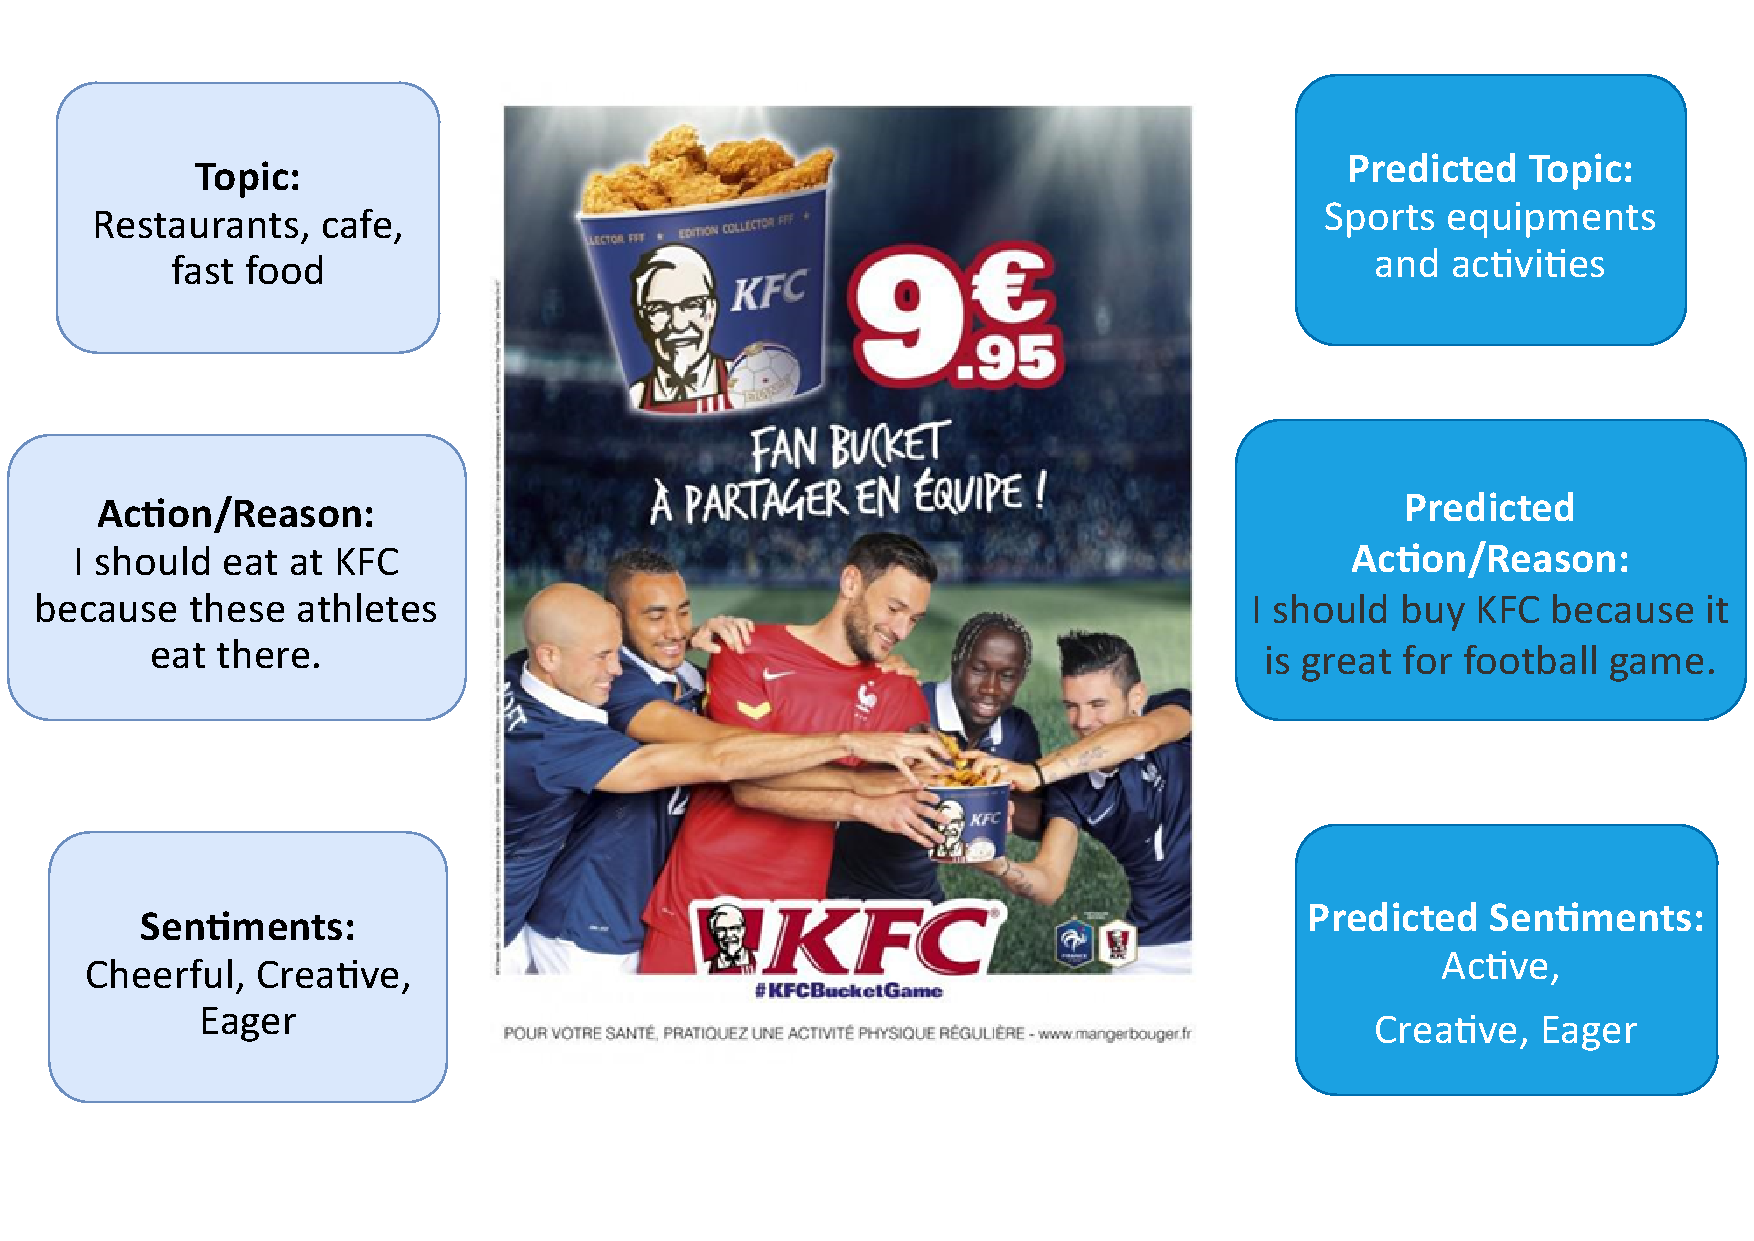
\includegraphics[width=\textwidth,scale=0.68]{images/preds_sup_8.pdf}
         \caption{}
         \label{fig:preds-sup-8}
            % \vspace{-10pt}
     \end{subfigure}
    \caption{Some samples from the Pitts Ads dataset along with the ground truth and predicted action-reason statement, topic and sentiments.}
    \label{fig:preds-sup}
\end{figure}


\subsubsection{Modelling Persuasion Strategy For Image Advertisements}
The proposed Ads dataset $\mathcal{D}$ annotated with the persuasion strategies comprises of samples where each sample advertisement $a_i$ is annotated with a set of annotation strategies $S_i$ such that $1\le|{S_i}|\le3$. The unique set of the proposed persuasion strategies $\mathcal{P}$ is defined in Table~\ref{tab:persuasive-strategies-list}. Given $a_i$, the task of the modeling is to predict the persuasion strategies present in the input ad. As we observe from Fig.~\ref{fig:persuasion-strategies-headline-image}, advertisements use various rhetoric devices to form their messaging strategy. The strategies thus are in the form of multi-modalities, including images, text and symbolism. To jointly model the modalities, we design an attention fusion multi-modal framework, which fuses multimodal features extracted from the ad, {\it e.g.}, the ad image, text present in the ad extracted through the OCR (Optical Character Recognition), regions of interest (ROIs) extracted using an object detector, and embeddings of captions obtained through an image captioning model (see Fig.~\ref{fig:arch_diag}). The information obtained through these modalities are firstly embedded independently through their modality specific encoders followed by a transformer-based cross-attention module to fuse the extracted features from different modalities. The fused embeddings from the attention module are then used as input for a classifier that predicts a probability score for each strategy $p \in \mathcal{P}$. The overall architecture of the proposed model is illustrated in Fig.\ref{fig:arch_diag}. In the following, we describe each step in the prediction pipeline in detail.


\paragraph{Feature Extractors} 

In order to capture different rhetoric devices, we extract features from the image, text, and symbolism modalities.

\textbf{Image Feature:} We use the Vision Transformer \cite{dosovitskiy2020image} (ViT) model for extracting image features from the entire input image. The model resizes the input image to size $224 \times 224$ and divides it into patches of size $16 \times 16$. The model used has been pre-trained on the ImageNet 21k dataset. We only use the first output embedding, which is the CLS token embedding, a $768$ dimension tensor, as we only need a representation of the entire image. Then, a fully connected layer is used to reduce the size of the embedding, resulting in a tensor of dimension $256$.




\textbf{Regions of Interest (RoIs) from Detected Objects and Captions:} %The major difference between creative and natural images is the presence of composing elements \cite{zitnick2013bringing,zitnick2014adopting}. 
Ad images contain elements that the creator deliberately chooses to create \textit{intentional impact} and deliver some \textit{message} in addition to the ones that occur \textit{naturally} in the environment. Therefore, it is important to identify the composing elements of an advertisement to understand the creator's intention and the ad's message to the viewer. We detect and extract objects as regions of interest (RoIs) from the advertisement images. We get the RoIs by training the single-shot object detector model \cite{liu2016ssd} on the COCO dataset \cite{lin2014microsoft}. We compare it with the recent YOLOv5 model \cite{redmon2016you}. We also extract caption embeddings to detect the most important activity from the image using a caption generation mode. We compare DenseCap \cite{yang2017dense} and the more recent BLIP \cite{li2022blip} for caption generation.




\textbf{OCR Text:} The text present in an ad presents valuable information about the brand, such as product details, statistics, reasons to buy the product, and creative information in the form of slogans and jingles that the company wants its customers to remember and thus making it helpful in decoding various persuasion strategies. Therefore, we extract the text from the ads and use it as a feature in our model. We use the Google Cloud Vision API for this purpose. All the extracted text is concatenated, and the size is restricted to $100$ words. We pass the text through a BERT model and concatenate the embeddings for those 100 words. Similar to image embeddings, an FC layer is used to convert embeddings to 256 dimensions. The final embedding of the OCR is a tensor of dimension $100 \times 256$. 


\textbf{Symbolism:} While the names of the detected objects convey the names or literal meaning of the objects, creative images often also use objects for their symbolic and figurative meanings. For example, an upward-going arrow represents growth or the north direction or movement towards the upward direction depending on the context; similarly, a person with both hands pointing upward could mean danger (\textit{e.g.}, when a gun is pointed) or joy (\textit{e.g.}, during dancing). In Fig.~\ref{fig:persuasion-strategies-headline-image}, in the creative Microsoft ad, a symbol of a balloon is created by grouping multiple mice together. Therefore, we generate symbol embeddings to capture the symbolism behind the most prominent visual objects present in an ad. We use the symbol classifier by Hussain \textit{et al.} \cite{hussain2017automatic} on ad images to find the distribution of the symbolic elements present and then convert this to a $256$ dimension tensor. %Finally we get a $2 \times 256$ dimension tensor.





\iffalse
{\small%
\begin{table}[]
\small
      \resizebox{0.8\columnwidth}{!}{%
      \begin{tabular}{ll}
            \toprule
             \textbf{Strategies} & \textbf{Corr}\\ \midrule
              Eager-Concreteness & 0.268 \\\midrule
             Scarcity-Reciprocity & 0.253 \\\midrule
             Eager-Cheerful  & 0.187 \\\midrule
             Amazed-Concreteness & 0.174 \\\midrule
             Eager-Reciprocity & 0.165 \\\bottomrule
        \end{tabular}}
        \caption{\looseness=-1 Top-5 Dice Correlated Persuasion Strategies. In general, we observe that persuasion strategies are not heavily correlated with each other. This means that the marketers are using unique combinations of messaging strategies to market their products.}
        \label{tab:top-5-correlated strategies}
    \end{table}}
\fi







\paragraph{Cross-Modal Attention} 
To capture the inter-dependency of multiple modalities for richer embeddings, we apply a cross-modal attention (CMA) layer~\cite{frank2021vision} to the features extracted in the previous steps. Cross-modal attention is a fusion mechanism where the attention masks from one modality (\textit{e.g.} text) are used to highlight the extracted features in another modality (\textit{e.g.} symbolism). It helps to link and extract common features in two or more modalities since common elements exist across multiple modalities, which complete and reinforce the message conveyed in the ad. For example, the pictures of the silver cup, stadium, and ball, words like ``Australian'', ``Pakistani'', and ``World Cup'' present in the chips ad shown in Fig.~\ref{fig:arch_diag} link the idea of buying \textit{Lays} with supporting one's country's team in the World Cup. Cross attention can also generate effective representations in the case of missing or noisy data or annotations in one or more modalities \cite{frank2021vision}. This is helpful in our case since marketing data often uses implicit associations and relations to convey meaning. 

The input to the cross-modal attention layer is constructed by concatenating the image, RoI, OCR, caption, and symbol embeddings. This results in a $114 \times 256$ dimension input to our attention layer. The cross-modal attention consists of two layers of transformer encoders with a hidden dimension size of $256$. %The rest of the hyper-parameters are similar to the ones given in the original paper \cite{vaswani2017attention}. 
The output of the attention layer gives us the final combined embedding of our input ad. 
Given image embeddings $E_i$, RoI embeddings $E_r$, OCR embeddings $E_o$, caption embeddings $E_c$ and symbol embeddings $E_s$, the output of the cross-attention layer $E_{att}$ is formulated as:
\begin{align}
        \text{Enc}(X) &= \text{CMA}(\left[E_i(X),E_r(X), E_o(X),E_c(X),E_s(X)\right])\,, \nonumber
\end{align}
where $[\ldots,\ldots]$ is the concatenation operation. For the advertisement in Fig.~\ref{fig:arch_diag}, we observed that the caption ``grey cup on the field'' attends to OCR text (containing words like ``win'') and ViT features of the RoI (of ``cup'' and ``field'').

%We propose solving the following tasks for understanding advertisements: action-reason generation, topic classification, and sentiment detection. For solving these, we consider a multi-task learning framework where each task has a task-specific network built upon a common, shared multi-modal encoder. We learn the shared parameters $\thetav_s$ and a set of task-specific parameters $\{\thetav_i\}^{T}_{i=1}$ for $T$ tasks. Our goal is to learn parameters $\thetav_s \cup \{\thetav_i\}^{T}_{i=1}$ that minimize loss across all tasks. Details on different tasks and loss designs are introduced next. In our specific setting, we have $T=3$.



\begin{landscape}
    
\begin{figure*}
% \vspace*{-11mm}
        \centering
        % \includegraphics[scale=0.28]{images/Model_Architecture.pdf}
        % \includegraphics[scale=0.185]{images/Persuasion Arch Diag - Copy of Model_Architecture-Page-2.drawio.png}
        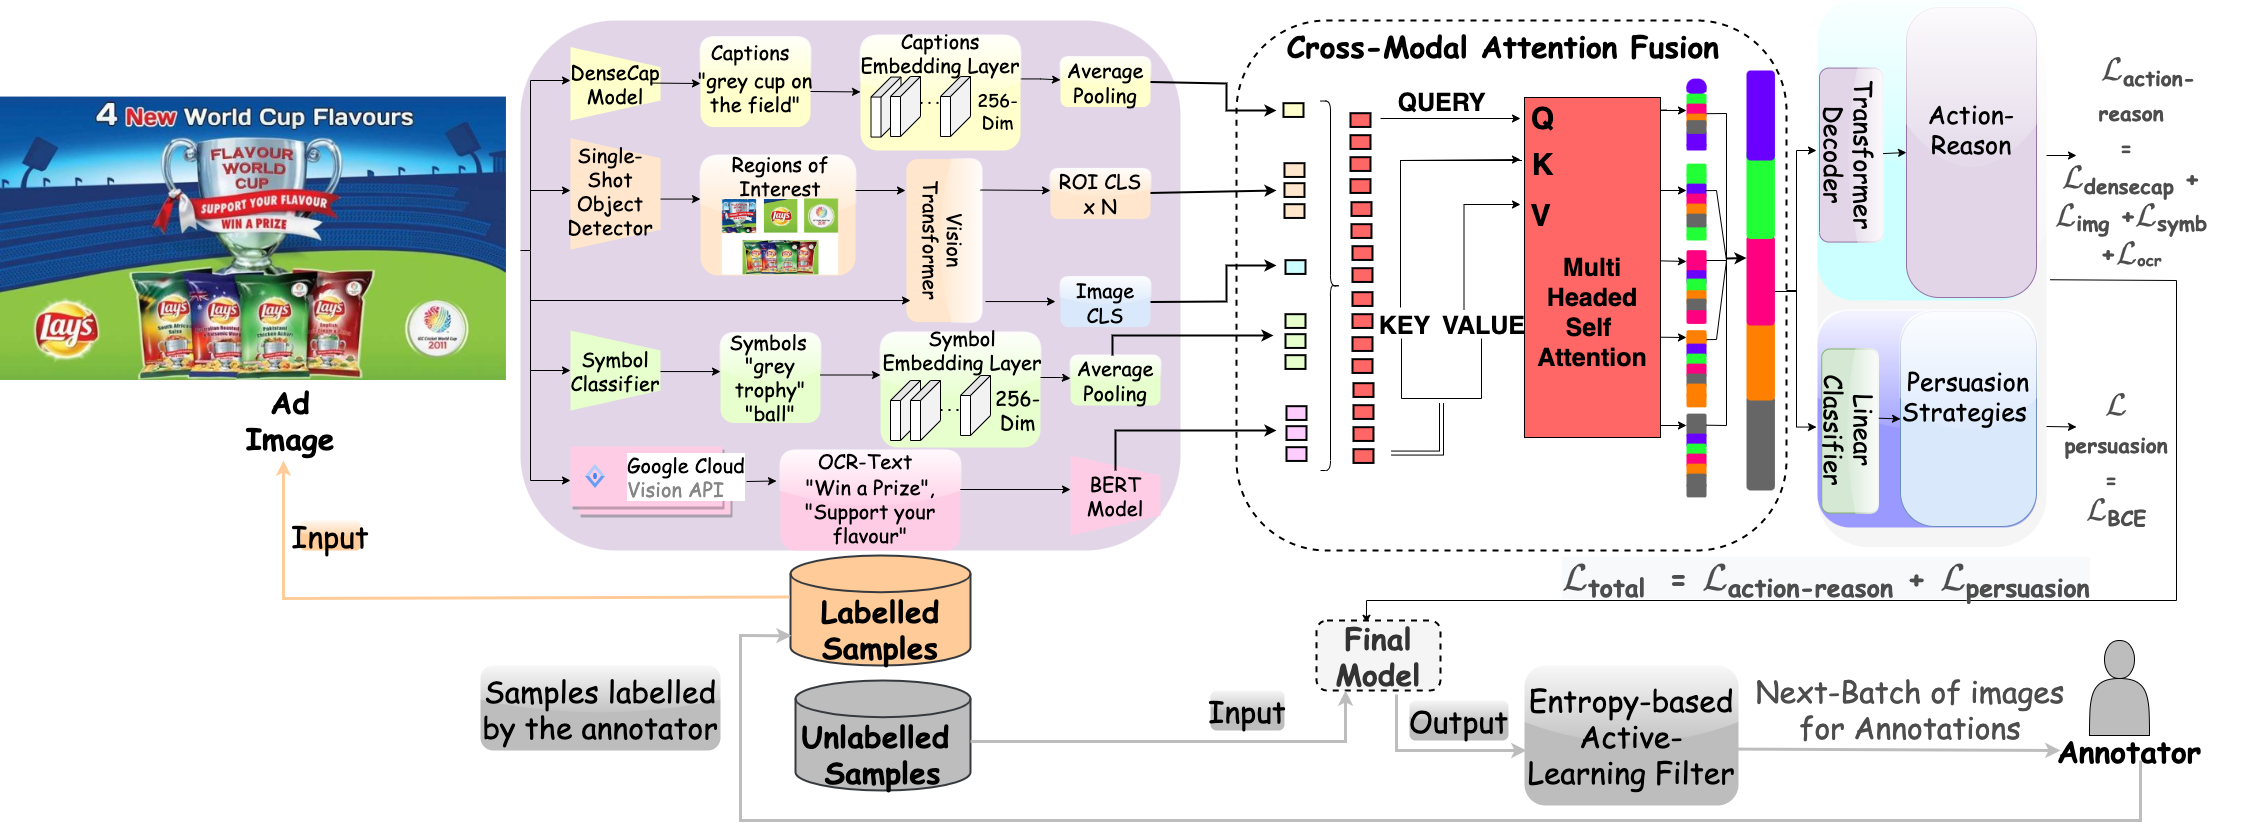
\includegraphics[width=1.5\textwidth]{images/Persuasion-Arch-Diag-Copy-of-Model_Architecture-Page-2.drawio.png}
        % \vspace*{-2mm}
        \caption{\small Architecture of the Persuasion Strategy Prediction model. To capture the different rhetoric devices, we extract features for the image, text, and symbolism modalities and then apply cross-modal attention fusion to leverage the interdependence of the different devices. Further, the model trains over two tasks: persuasion strategies and the reasoning task of action-reason prediction.}
        % \label{fig:persuasion-strategies-headline-image}
% \vspace*{-4mm}
\label{fig:arch_diag}
\end{figure*}
\end{landscape}


\paragraph{Persuasion Strategy Predictor} 
This module is a persuasion strategy predictor, which processes the set of feature embedding \text{Enc}(X) obtained through cross-modality fusion. Specifically, \text{Enc}(X) is passed through a self-attention layer as:
\begin{align}
o_{1} = softmax(\text{Enc}(X) \otimes W_{self-attn})^\intercal \otimes \text{Enc}(X)
\end{align}
where \text{Enc}(X) is of the dimension $114\times256$,  $W_{self-attn} \in \mathcal{R}^{256 \times 1}$, $\otimes$ denote tensor multiplication and $o_1$ denotes the output of self attention layer, which is further processed through a linear layer to obtain $o_{|\mathcal{P}|}$ to represent the logits for each persuasion strategy. We apply sigmoid over each output logit such that the $i^{th}$ index of the vector after applying sigmoid denotes $p_i$ - the probability with which $i^{th}$ persuasion strategy is present in the ad image. Our choice of using sigmoid over softmax is motivated by the fact that multiple persuasion strategies can be present simultaneously in an ad image. Consequently, the entire model is trained in an end-to-end manner using binary cross-entropy loss $\mathcal{L}_{s}$ over logit for each strategy:
\begin{align}
        \mathcal{L}_{s} = \left[-y_i \log(p_i) - (1-y_i) \log(1 - p_i) \right]
\end{align}
where, $y_i$ is 1 if $i^{th}$ persuasion strategy is present in the ad and 0 otherwise. It can be observed in Table~\ref{tab:modalities} that our model achieves an accuracy of $59.2\%$, where a correct match is considered if the strategy predicted by the model is present in the set of annotated strategies for a given ad. Further, we perform several ablations where we exclude each modality while retaining all the other modalities. We note that for each modality, excluding the modality results in a noticeable decrease in accuracy, with significant decreases observed when excluding DenseCap ($\sim3.6\%$) and OCR ($\sim4.4\%$). Further, we observe that using DenseCap for obtaining caption embeddings, and SSD for object detection works better than BLIP and YOLOv5, respectively (see Table~\ref{tab:varying_cap_obj}). We also explore using focal loss~\cite{lin2017focal} in place of cross-entropy loss to handle class imbalance but observed that it led to degradation instead of improvements (top-1 acc.\footnote{\textit{Top-1 Accuracy}: It is defined as the fraction of images, where the highest predicted strategy is present in the ground-truth strategies. \textit{Top-3 Accuracy} : It is defined as the fraction of images, where any of the top-3 highest predicted strategies is present in the ground-truth strategies.} of $56.4\%$ \textit{vs} $59.2\%$ using cross-entropy). We also train the model of Hussain \textit{et al.} \cite{hussain2017automatic} for strategy prediction through a similar configuration as ours (along with action-reason generation using an LSTM branch). We find that their top-1 and top-3 accuracy is 52.4\% (vs. 59.2\% ours) and 75.7\% (vs. 84.8\% ours), which is lesser compared to our model.

\begin{table}[t]
% \vspace{-8mm}
    \small
        \centering
        %\begin{adjustbox}{width=\columnwidth,center}
        \resizebox{0.5\columnwidth}{!}{%
       \begin{tabular}{lll}%[tab1,tabularx={XYYYYY}]
             \textbf{\thead{Models}} & \textbf{\thead{Top-1  Acc.}} & \textbf{\thead{Top-3 Acc.}}\\ \midrule
             Our Model & \textbf{59.2} & \textbf{84.8} \\ \midrule
             w/o DenseCap & 55.6 & 80.8 \\ \midrule
             w/o Symbol   & 58.8 & 81.6 \\ \midrule
           w/o DenseCap \& Symbol & 55.2 & 80.8 \\ \midrule
            w/o OCR & 54.8 & 82 \\ \midrule
            w/o Symbol,\\OCR \& DenseCap & 58 & 78.8 \\ \midrule
                %  With Topic & 43.2 & 67.2 \\ \bottomrule
            w/o Action-Reason Task & 56.4 & 80.4\\ \midrule
            Random Guess & 6.25 &  18.75\\\bottomrule
        \end{tabular}}
        \caption{\small Effect of different Modalities and Tasks on the accuracy and performance of the strategy prediction task.}
        % \vspace{-3mm}
        %\end{adjustbox}
        \label{tab:modalities}
    \end{table}

\paragraph{Multi Task Learning}
One of the key opportunities for our persuasion strategies data labeling and modeling task was the presence of additional labels already given in the base Pitts Ads dataset. In that, authors had given labels about the reasoning task. For the reasoning task, the annotators were asked to provide answers in the form ``I should [Action] because [Reason]." for each ad. In other words, they asked the annotators to describe \textit{what the viewer should do and why}, according to
the ad. Similar to the reasoning task, persuasion strategies provide various cognitive, behavioral, and affective reasons to try to elicit the motivation of the ad viewers towards their products or services. Therefore, we hypothesize that these natural language descriptions of \textit{why the viewers should follow} the ad will be informative in inferring the ad's persuasion strategy.

We formulate obtaining action-reason statement as a sequence generation task where the model learns to generate a sentence $Y^g=(y^g_1, \ldots, y^g_T)$ of length $T$ conditioned on advertisement $X$ by generating the sequence of tokens present in the action-reason statement. To achieve this, we use a transformer decoder module that attends on the features $\text{Enc}(X)$ as shown in Fig.~\ref{fig:arch_diag}. The annotated action-reason statement is used to train the transformer decoder as an auxiliary task to strategy prediction through the standard teacher forcing technique used in Seq2Seq framework. Please refer to the Supplementary for more architectural details about the action-reason generation branch. As shown in Table~\ref{tab:modalities}, generating action-reason as an auxiliary task improves the strategy prediction accuracy by $2.8\%$. We evaluate the performance on action-reason generation on following metrics: BLEU-1, BLEU-2, BLEU-3, BLEU-4, METEOR, ROUGE, CIDER, SPICE and observed a score of 53.6, 42.0, 33.1, 25.7, 26.3, 48.4, 42.8, 8.9 respectively.


% task Ti dataset Di consisting  of ni training  samples,  i.e.,Di={xij,yij}nij=1,  where xij∈Rdi is the jth training instance in Ti and yi ji s its label. We denote byXithe  training  data  matrix  forTi,  i.e.,Xi= (xi1,...,xini)

% \vspace{-1mm}

\begin{table}[!t]
        \small
        \centering
        % \vspace{-8mm}

        %\begin{adjustbox}{width=\columnwidth,center}
        \resizebox{0.55\columnwidth}{!}{%
       \begin{tabular}{llllll}%[tab1,tabularx={XYYYYY}]
                \textbf{\thead{Model Used}} & \textbf{\thead{Top-1 \\Accuracy}} & \textbf{\thead{Top-3 \\Accuracy}} &  \textbf{Recall} \\ \midrule
                 Model with \\DenseCap \& SSD & 59.2 & 84.8 & 74.59\\ \midrule
                 Model with \\BLIP \& YOLOv5 & 58.4 &  83.8 & 71.58 \\ \midrule
        \end{tabular}}
        \caption{\small Comparison of caption and object detection models. We noticed that BLIP while being more recent and trained on a larger dataset, generates more informatory captions for background objects which DenseCap successfully ignores.}
        % \vspace{-3mm}
        %\end{adjustbox}
        \label{tab:varying_cap_obj}
    \end{table}
        \begin{figure}[h]
        \centering
        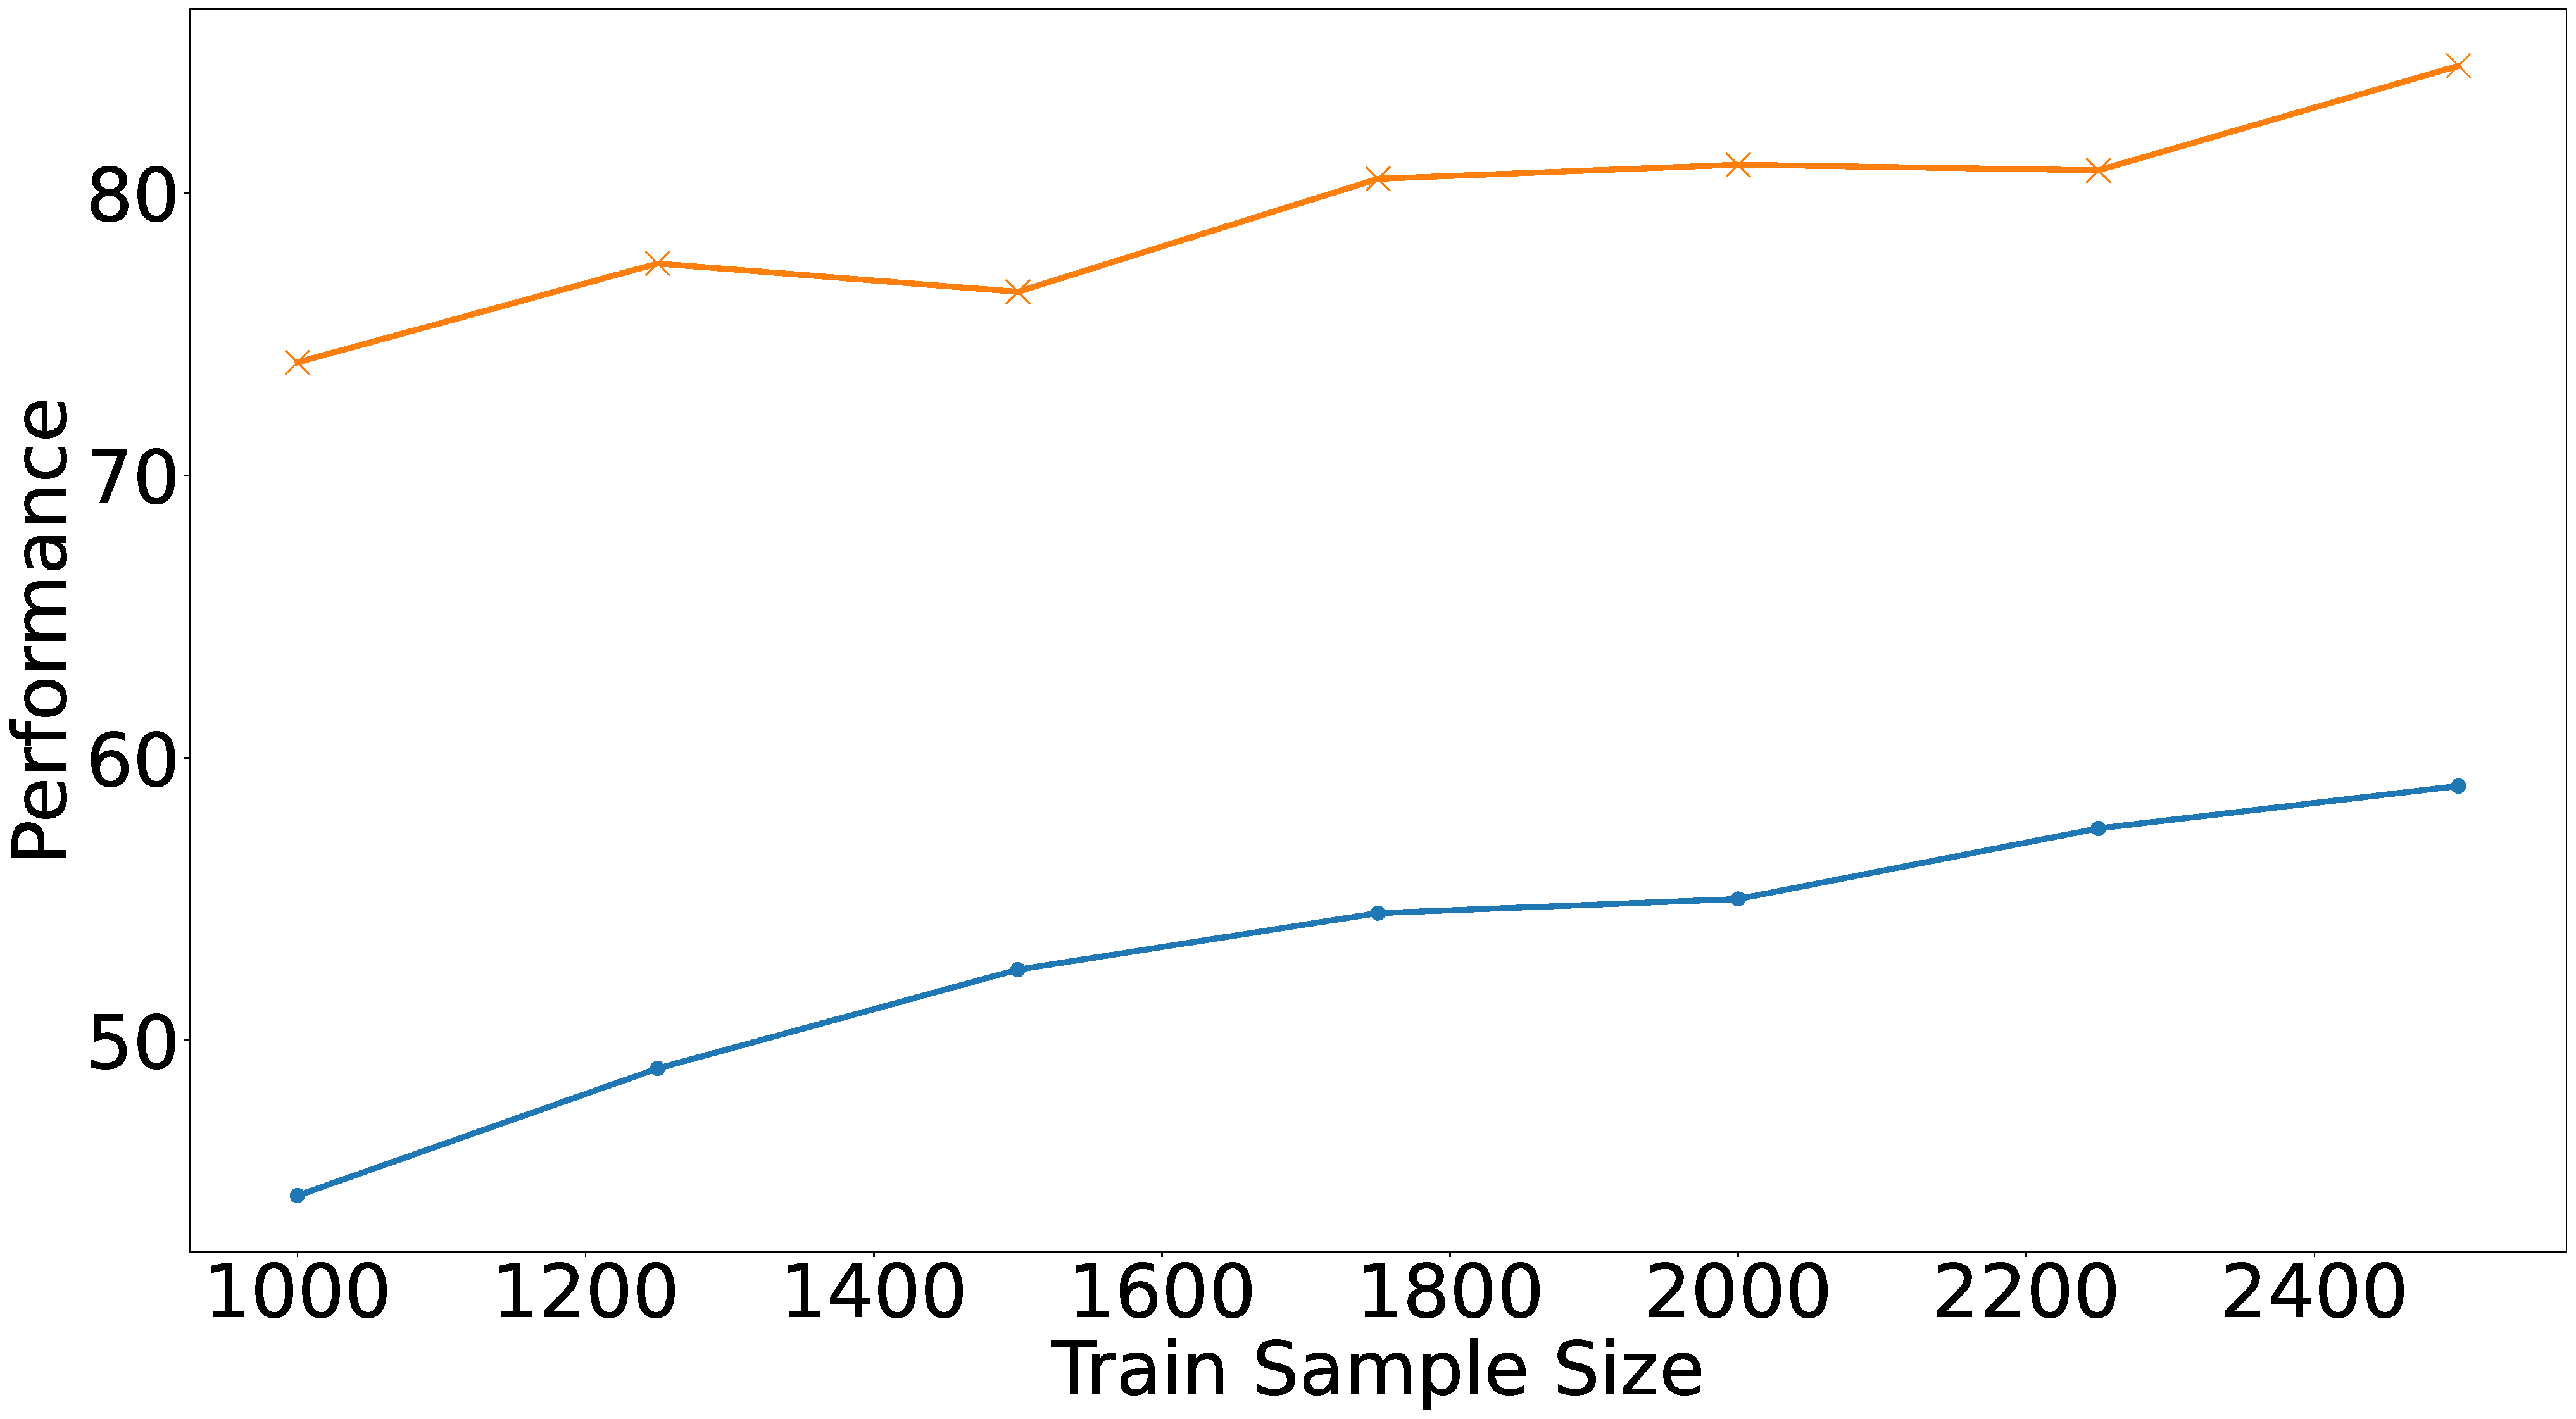
\includegraphics[scale=0.12]{images/active_learning.pdf}
        \caption{\small Incremental effect of introducing new data through active learning; Results for prediction of persuasion strategies on the test set}
        % \vspace{-4mm}
        \label{fig:AL_batch_test}
    \end{figure}


\begin{table}[]
    \small
        \centering
        %\begin{adjustbox}{width=\columnwidth,center}
        \resizebox{0.8\textwidth}{!}{%
       \begin{tabular}{llllll}%[tab1,tabularx={XYYYYY}]
             & \textbf{\thead{\#ads with \\1 strategy}} & \textbf{\thead{\#ads with \\2 strategies}} & \textbf{\thead{\#ads with \\3 strategies}} & \textbf{\thead{Avg.\\strategies}} & \textbf{\thead{Std.\\Dev.}}\\ \midrule
             Train-Set & 1440 & 905 & 155 & 1.486 & 0.612 \\\midrule
             Val-Set & 132 & 98 & 20 & 1.552  & 0.639 \\\midrule
             Test-Set & 147 & 93 & 10 & 1.452 &0.574\\\midrule\midrule
             Total & 1719 & 1096 & 185 & 1.49 & 0.592 \\\bottomrule
        \end{tabular}}
        \caption{\small Distribution of test, train, validation, and the total dataset}
        \label{table:strategy-train-test-val-stats}
        % \vspace*{-3mm}
        %\end{adjustbox}
    \end{table}



\paragraph{Active Learning}
We use an active learning method to ease the large-scale label dependence when constructing the dataset. As in every active learning setting, our goal is to develop a learner that selects samples from unlabeled sets to be annotated by an oracle. Similar to traditional active learners \cite{gilad2005query,lewis1994heterogeneous}, we use uncertainty sampling to perform the sample selection. In doing so, such function learns to score the unlabeled samples based on the expected performance gain they are likely to produce and used to update the current version of the localization model being trained. To evaluate each learner, we measure the performance improvements, assessed on a labeled test set at different training dataset sizes.


At every learning step $t$, a set of labeled samples $L_t$ is first used to train a model
$f_t$. Then, from an unlabeled pool $U_t=D-L_t$, an image instance $a$ is chosen by a selection function $g$. Afterwards, an oracle provides temporal ground-truth for the selected instance, and the labeled set $L_t$ is augmented with this new annotation. This process repeats until the desired performance is reached or the set $U_t$ is empty.

In our implementation, we instantiate the active learning selection function as the entropy of the probability distribution predicted by the model over the set of persuasion strategies for a given ad image instance $a$. Formally, $g = -\sum_{i=1}^{|\mathcal{P}|}p^{n}_{i}*\log(p^{n}_i)$, where $p^{n}_i$ denotes the normalized probability with which $i^{th}$ persuasion strategy is present in $a$ as per the model prediction. The normalized probability $p^{n}_{i}$ is estimated as $p_i/\sum_{j=1}^{|\mathcal{P}|}p_j$. Intuitively, ad samples with high entropy selection values indicate that the model trained on limited data has a higher degree of confusion while predicting the persuasion strategy since it is not decisively confident about predicting few strategies. Hence, we rank the unlabeled ad images in the decreasing order of difficulty according to the corresponding values of the entropy selection function and select the top-k ads in the subsequent batch for annotation followed by training. As shown in Fig.~\ref{fig:AL_batch_test}, we set k to be 250 and analyze the effect of incrementally introducing new samples selected through active learning. It can be seen that both top-1 and top-3 accuracy increases with the addition of new training data. We stop at the point when 2500 training samples are used since the model performs reasonably well with a top-1 and top-3 strategy prediction accuracy of 59.2\% and 84.8\% (see Fig.~\ref{fig:AL_batch_test}). 


For sample selection, we rank the ads using the model's entropy as the ranking function. We choose samples with the highest entropy, indicating the model's confusing in predicting strategies. The ad samples with top-k entropy (where k=250) are selected for annotation in each batch (with the entropy thresholds for each batch being determined by the entropy of the kth sample). The active learning process stops when the model achieves reasonable performance (thus determining the convergence criterion), with a top-1 accuracy of 59.2\% and top-3 accuracy of 84.8\% after training on 2,500 samples. Incremental improvements in accuracy are observed as new data is introduced through active learning.





%%%%%%%%%%%%%%%%%%%%%%%%%%%%%%%%%%%%%%%%%%%%%%%%%%%%%%%%%%%%%%%%%%%%
%%%%%%%%%%%%%%%%%%%%%%%%%%%%%%%%%%%%%%%%%%%%%%%%%%%%%%%%%%%%%%%%%%%%



\subsubsection{Modelling Persuasion Strategy For Video Advertisements}
Large Language Models (LLMs) have been demonstrated to perform well for downstream classification tasks in the text domain. This powerful ability has been widely verified on natural language tasks, including text classification, semantic parsing, mathematical reasoning, \textit{etc}. Inspired by these advances of LLMs, we aim to explore whether they could tackle reasoning tasks on multimodal data (\textit{i.e.} videos). Therefore, we propose a storytelling framework, which leverages the power of LLMs to verbalize videos in terms of a text-based story and then performs downstream video understanding tasks on the generated story instead of the original video. Our pipeline can be used to verbalize videos and understand videos to perform complex downstream tasks such as emotion, topic, and persuasion strategy detection. 


We show the performance of our framework on fifteen distinct tasks across five datasets. Firstly, we employ a video story dataset to evaluate the story generation task. Secondly, we utilize a video advertisements dataset to assess topic and emotion classification, as well as action and reason generation. Then, the persuasion strategy dataset to evaluate the task of understanding persuasion strategies within stories, and finally, HVU and LVU for concept, user engagement, and attribute prediction. These diverse datasets allow us to evaluate the performance and capabilities of our framework thoroughly.


\textbf{1.~The Video story dataset} \cite{Li_2020} contains 105 videos, from four types of common and complex events (\textit{i.e.} birthday, camping, Christmas, and wedding) and corresponding stories written by annotators. It has longer videos (average length 12.4 mins) and longer descriptions (162.6 words on average).
Moreover, the sentences in the dataset are more sparsely distributed across the video (55.77 sec per sentence).
\textit{Metrics}: Following \cite{Li_2020}, we use several NLP metrics, \textit{viz.}, BLEU-N, ROUGE-L, METEOR and CIDEr to measure the similarity between the story generated by the model and ground truth.


\textbf{2.~The Image and Video Advertisements} \cite{hussain2017automatic} contains 3,477 video advertisements and the corresponding annotations for emotion and topic tags and action-reason statements for each video. There are a total of 38 topics and 30 unique emotion tags per video. Further, we have 5 action-reason statements for each video for the action-reason generation task. For our experiment, we use 1785 videos, due to other videos being unavailable/privated from Youtube.

\textit{Metrics}: Following \cite{hussain2017automatic}, for the topic and emotion classification task, we evaluate our pipeline using top-1 accuracy as the evaluation metric. Further, since \cite{hussain2017automatic} did not use any fixed set of vocabulary for annotations, rather they relied on annotator-provided labels, the labels are often very close (like cheerful, excited, and happy). Therefore, based on nearness in Plutchik's \cite{PLUTCHIK19803} wheel of emotions, we club nearby emotions and use these seven main categories: joy, trust, fear, anger, disgust, anticipation, and unclear. For the action-reason task, following \cite{hussain2017automatic}, we evaluate our accuracy on the action and reason retrieval tasks where 29 random options along with 1 ground truth are provided to the model to find which one is the ground truth. Further, we also generate action and reason statements and evaluate the generation's faithfulness with the ground truth using metrics like ROUGE, BLEU, CIDEr, and METEOR.


\textbf{3.~Persuasion strategy dataset}: This is the dataset we contribute for understanding persuasion strategies.

\textit{Metrics}: We evaluate the performance using top-1 accuracy metric. Videos have a varied number of strategies, therefore, we consider a response to be correct if the predicted strategy is present among the list of ground-truth strategies.


\textbf{4.~Long-Form Video Understanding (LVU)}: We \textit{et al.} \cite{wu2021towards} released a benchmark comprising of 9 diverse tasks for long video understanding and consisting of over 1000 hours of video. The various tasks consist of content understanding (`relationship', `speaking style', `scene/place'), user engagement prediction (`YouTube like ratio', `YouTube popularity'), and movie metadata prediction (`director', `genre', `writer', `movie release year'). We \textit{et al.} \cite{wu2021towards} use top-1 classification accuracy for content understanding and metadata prediction tasks and MSE for user engagement prediction tasks.


\textbf{5.~Holistic Video Understanding (HVU)}: 
HVU \cite{diba2020large} is the largest long video understanding dataset consisting of 476k, 31k, and 65k samples in train, val, and test sets, respectively. A comprehensive spectrum includes the identification of various semantic elements within videos, consisting of classifications of scenes, objects, actions, events, attributes, and concepts. To measure performance on HVU tasks, similar to the original paper, we use the mean average precision (mAP) metric on the validation set.



Next, we explain our pipeline to solve these tasks.

\paragraph{Video Verbalization} 
To obtain a verbal representation of a video, we employ a series of modules that extract unimodal information from the multimodal video. This information is then used to prompt a generative language model (such as GPT-3.5 \cite{brown2020language} and Flan-t5 \cite{chung2022scaling}) to generate a coherent narrative from the video. The overall pipeline is depicted in Fig.~\ref{fig:story-generation-pipeline}. In the following, we delve into each component of the framework in details.

\noindent \textbf{1. Video Metadata:} Understanding the context of a story is crucial, and we achieve this by gathering information about the communicator (brand). We leverage the publicly available video title and channel name from the web. Additionally, we utilize Wikidata \cite{10.1145/2629489}, a collaborative knowledge base that provides comprehensive data for Wikipedia, to obtain further details such as the company name, product line, and description. This information helps us comprehend the story elements and establish connections with the brand's business context. For non-advertisement videos, we skip this step and retrieve only the video title.

\noindent \textbf{2. Text Representation of Video Frames:} We extract two types of textual information from video frames. Firstly, we capture the literal text present on the frames. Secondly, we analyze the scene depicted in each frame to gain a deeper understanding. In the upcoming sections, we will elaborate on both of these aspects.


\begin{table*}[!h]\centering
% \scriptsize
\begin{adjustbox}{width =\textwidth}
\begin{tabular}{llccccccc}\toprule[1.5pt]
\textbf{Method} &\textbf{Frame Extraction} &\textbf{METEOR} & \textbf{CIDEr} &\textbf{Rougle-l} &\textbf{BLEU-1}&\textbf{BLEU-2}&\textbf{BLEU-3}&\textbf{BLEU-4}\\\toprule[0.5pt]
GPT-3.5 & Uniform Sampling & 24.8 & 102.4 & 24.3 & 63.8 & 56.4 & 47.2 & 38.6 \\
GPT-3.5 & Pyscenedetect & 24.17 & 67.8 & 21.17 & 54.59 & 49.05 & 41.54 & 33.88 \\\bottomrule[1.5pt]
\end{tabular}
\end{adjustbox}
\caption{Comparison of Pyscenedetect \cite{breakthrough-pyscenedetect} with uniform sampling of choosing video frames. Based on downstream performance, we can see that uniform sampling works better than Pyscenedetect  \label{tab:ablation-sampling}}
\end{table*}

\textit{a. Visual and Scenic Elements in Frames:} For videos with a duration shorter than 120 seconds, we employ an optical flow-based heuristic using the GMFlow model \cite{xu2022gmflow} to extract keyframes. In shorter advertisement videos, scene changes often indicate transitions in the story, resulting in keyframes with higher optical flow values. The GMFlow model effectively captures these story transitions. We select frames with an optical flow greater than 50 and prioritize frames with maximum pixel velocity. However, for longer videos, this approach yields a large number of frames that are difficult to accommodate within a limited context. To address this, we sample frames at a uniform rate based on the native frames-per-second (fps) of the video (see Table~\ref{tab:ablation-sampling} for a comparison between uniform sampling and Pyscenedetect). Additionally, we discard frames that are completely dark or white, as they may have high optical flow but lack informative content.

Using either of these methods, we obtain a set of frames that represent the events in the video. These frames are then processed by a pretrained BLIP-2 model \cite{li2023blip2}. The BLIP model facilitates scene understanding and verbalizes the scene by capturing its most salient aspects. We utilize two different prompts to extract salient information from the frames. The first prompt, ``\textit{Caption this image}", is used to generate a caption that describes what is happening in the image, providing an understanding of the scene. The second prompt, ``\textit{Can you tell the objects that are present in the image?}", helps identify and gather information about the objects depicted in each frame.



\begin{figure*}[!t]
    \centering
    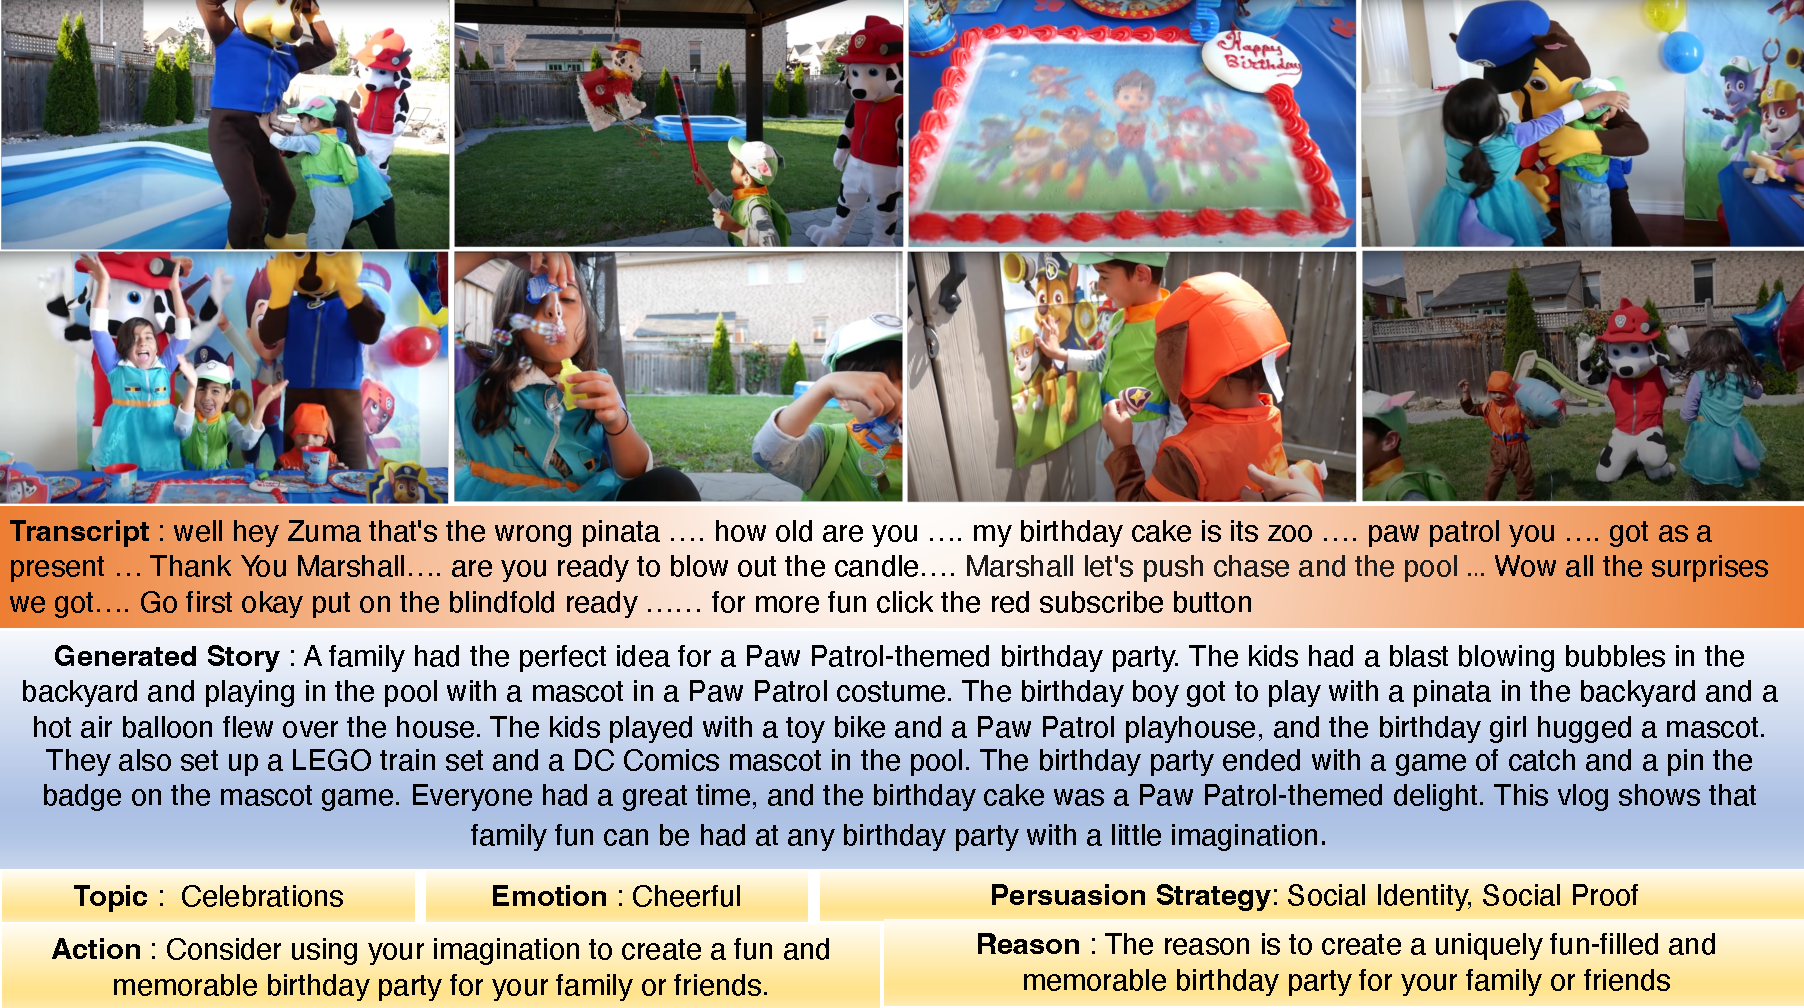
\includegraphics[width=\textwidth]{images/example-stories.pdf}
    \caption{An example of a story generated by the proposed pipeline along with the predicted outputs of the video-understanding tasks on the generated story. The generated story captures information across scenes, characters, event sequences, dialogues, emotions, and the environment. This helps the downstream models to get adequate information about the video to reason about it correctly. The original video can be watched at \url{https://youtu.be/_amwPjAcoC8}.}
    \label{fig:example-story}
\end{figure*}


\textit{b. Textual elements in frames:} We also extract the textual information present in the frames, as text often reinforces the message present in a scene and can also inform viewers on what to expect next \cite{9578608}. 
For the OCR module, we sample every 10th frame extracted at the native frames-per-second of the video, and these frames are sent to PP-OCR \cite{10.1145/2629489}. We filter the OCR text and use only the unique words for further processing.

\noindent \textbf{3. Text Representation of Audio:} The next modality we utilize from the video is the audio content extracted from it. We employ an Automatic Speech Recognition (ASR) module to extract transcripts from the audio. Since the datasets we worked with involved YouTube videos, we utilized the YouTube API to extract the closed caption transcripts associated with those videos.

\noindent \textbf{4. Prompting:} We employ the aforementioned modules to extract textual representations of various modalities present in a video. This ensures that we capture the audio, visual, text, and outside knowledge aspects of the video. Once the raw text is collected and processed, we utilize it to prompt a generative language model in order to generate a coherent story that represents the video. To optimize the prompting process and enable the generation of more detailed stories, we remove similar frame captions and optical character recognition (OCR) outputs, thereby reducing the overall prompt size. %\cy{Do we simply concantenate all the text as the prompt? in what order?}


\begin{landscape}
\begin{figure*}
  \includegraphics[width=1.5\textwidth]{images/verbalizing-marketing-graphics.pdf}
  \caption{The overview of our framework to generate a story from a video and perform downstream video-understanding tasks. First, we sample keyframes from the video which are verbalized using BLIP-2. We also extract OCR from all the frames. Next, using the channel name and ID, we query Wikidata to get company and product information. Next, we obtain automatically generated captions from Youtube videos using the Youtube API. All of these are concatenated as a single prompt and given as input to an LLM and ask it to generate the story of the advertisement. Using the generated story, we then perform the downstream tasks of emotion and topic classification and persuasion strategy identification. This video can be watched at \url{https://youtu.be/ZBLkTALi1CI}.
  %\url{https://github.com/Aanisha/persuasion-advertisements/blob/main/videos/ZBLkTALi1CI.mp4}.
  }
  \label{fig:story-generation-pipeline}
\end{figure*}
\end{landscape}








The prompt template is given in Section~\ref{sec:prompt-format}. Through experimentation, we discovered that using concise, succinct instructions and appending the text input signals (such as frame captions, OCR, and automatic speech recognition) at the end significantly enhances the quality of video story generation. For shorter videos (up to 120 seconds), we utilize all available information to prompt the LLM for story generation. However, for longer videos, we limit the prompts to closed captions and sampled frame captions. The entire prompting pipeline is zero-shot and relies on pre-trained LLMs. In our story generation experiments, we employ GPT-3.5 \cite{brown2020language}, Flan-t5 \cite{chung2022scaling}, and Vicuna \cite{vicuna2023}. A temperature of 0.75 is used for LLM generation. The average length of the generated stories is 231.67 words. Subsequently, these generated stories are utilized for performing video understanding tasks.



\paragraph{Prompt format} 
\label{sec:prompt-format}
 For verbalization, a template prompt format has been used, including all the data components as objects, captions, asr, ocr, meta-data. 

\textit{``Please write a coherent story based on the following video advertisement. Use only the information provided and make sure the story feels like a continuous narrative and at the end include one sentence about what product the advertisement was about. Do not include any details not mentioned in the prompt.Use the elements given below to create a coherent narrative,but don't use them as it is.The advertisement for the company \{company\_name\} The video is titled \{title\}, with captions that include \{caption\}, voice-over : \{transcripts\}, and object recognition descriptions : \{ocr\}. The following objects are present in the advertisement and should be used to help create the story: \{objects\} Please exclude any empty or stop words from the final text.''}

For downstream tasks, a template prompt format with an instruction about the specific task,the previous generated verbalization and vocabulary for the downstream task is prompted to the LLM. Here is the example for the topic detection task, for other tasks context and vocab were changed accordingly.

\textit{``Given \{topics\} identify the most relevant topic from the dictionary keys from topic\_vocab related to the story of the video advertisement given below.Consider the definitions given with topics in the topic\_vocab dictionary, to identify which topic is most relevant, don't add any extra topics that are not given in dictionary keys and answer with just the most relevant topic. Story : \{verbalization\}''}


\begin{table*}[!h]\centering
% \scriptsize
\begin{adjustbox}{width=\textwidth}
\begin{tabular}{llccccccc}\toprule[1.5pt]
\multirow{2}{*}{\textbf{Training}} & \multirow{2}{*}{\textbf{Model}} &\textbf{Topic} &\multicolumn{2}{c}{\textbf{Emotion}} & \textbf{Persuasion} &\textbf{Action} &\textbf{Reason}\\\cmidrule{4-5}
& & & \textbf{All labels} & \textbf{Clubbed} \\ \midrule[0.5pt]
Random & Random & 2.63 & 3.37 & 14.3 & 8.37 & 3.34 & 3.34 \\\hline
Finetuned & VideoMAE \cite{tong2022videomae} & 24.72 & 29.72 & \valgood{85.55}  & 11.17  & - & - \\
& Hussain \textit{et al.} \cite{hussain2017automatic} & 35.1 & 32.8 & -  & - & - & 48.45 \\
\ & Intern-Video \cite{wang2022internvideo} & 57.47 & \valbest{36.08} & \valbest{86.59} & 5.47 & 6.8 & 7.1 \\\hline
Zero-shot & VideoChat \cite{li2023videochat} & 9.07 & 3.09 & 5.1 &  10.28 & - & - \\

\hline
\textbf{Our Framework} & \makecell{GPT-3.5 Generated Story +\\GPT-3.5 Classifier} & 51.6 & 11.68 & 79.69 &  35.02 &  66.27 & 59.59 \\
Zero-shot & \makecell{GPT-3.5 Generated Story +\\Flan-t5-xxl Classifier} & \valgood{60.5} & 10.8 & 79.10 &  \valgood{33.41} &  \valbest{79.22} & \valbest{81.72} \\
& \makecell{GPT-3.5 Generated Story +\\Vicuna Classifier} & 22.92 & 10.8 & 67.35 & 29.6 & 21.39 & 20.89 \\
& \makecell{Vicuna Generated Story +\\GPT-3.5 Classifier} & 46.7 & 5.9 & 80.33 & 27.54 & 61.88 & 55.44 \\
& \makecell{Vicuna Generated Story +\\Flan-t5-xxl Classifier} & 57.38 & 9.8 & 76.60 & 30.11 & \valgood{77.38} & \valgood{80.66}  \\
& \makecell{Vicuna Generated Story +\\Vicuna Classifier} & 11.75 & 10.5 & 68.13 & 26.59 & 20.72 & 21.00  \\\cmidrule{2-8}
Finetuned & \makecell{Generated Story +\\Roberta Classifier} & \valbest{71.3} & \valgood{33.02} & 84.20 & \valbest{64.67} & 42.96\footnotemark[1] & 39.09\footnotemark[1] \\
% & BLIP-2 Captions + Flant-t5-xl & 32.2 & 7.4 & 43.11 &  32.1 & 52.98 & 76.26 \\
% & BLIP-2 Captions + GPT-3.5 & 32.7 & 7.9 & 76.3 & 30.1 & 49.91 & 58.71 \\

\bottomrule[1.5pt]
\end{tabular}
\end{adjustbox}
\caption{Comparison of all the models across topic, emotion, and persuasion strategy detection tasks. We see that our framework, despite being zero-shot, outperforms finetuned video-based models on the topic classification, persuasion strategy detection and action and reason classification tasks and comes close on the emotion classification task. Further, the Roberta classifier trained on generated stories outperforms both finetuned and zero-shot models on most tasks. Best models are denoted in \valbest{green} and runner-ups in \valgood{blue}.\label{tab:topic-sentiment}}
\end{table*}



\begin{table*}[!th]
  \centering
  % \begin{tabular}{cccccccccc}
  \begin{adjustbox}{width=\textwidth}
  \begin{tabular}{cccccccccc}
    \toprule
    & Method & Model Type & METEOR & CIDEr & ROUGE-L & BLEU-1 & BLEU-2 & BLEU-3 & BLEU-4 \\
    \midrule
    
    Random & Random  & Retrieval  & 13.1 & 30.2 & 21.4 & 43.1 & 23.1 & 10.0 & 4.8 \\\hline
    %\textbf{Finetuned} & CCA \cite{5540112} & Retrieval & 16.5 & 71.8 & 26.7 & 60.1 & 34.7 & 11.8 & 10.1 \\
    %& Uniform \cite{Li_2020}  & Retrieval & 18.3 &  89.9 & 28.0 & 65.7 & 40.6 & 23.2 & 13.2 \\
    %& SeqDPP \cite{NIPS2014_0eec27c4}  & Retrieval & 18.3 & 91.6 & 28.3 & 66.3 & 41.0 & 23.6 & 13.1 \\
    %& Submodular \cite{7298928} & Retrieval & 18.4 & 92.0 & 28.1 & 66.4 & 41.0 & 23.8 & 13.3 \\
    %& vsLSTM \cite{zhang2016video} & Retrieval & 18.2 & 92.4 & 28.2 & 66.6 & 41.5 & 24.1 & 13.6 \\
    %\textbf{Finetuned} & Narrator IoU \cite{Li_2020} & Retrieval & 18.6 & 93.7 & 28.2 & 67.9 & 42.1 & 24.7 & 14.1 \\
    %& Narrator w/o x \cite{Li_2020} & Retrieval & 18.5 & 93.4 & 28.3 & 67.3 & 41.6 & 24.5 & 14.2 \\
    %\textbf{Finetuned} & Narrator w/o f\_(l) \cite{Li_2020} & Retrieval & 19.0 & 96.1 & 29.1 & 68.6 & 42.9 & 25.2 & 14.5 \\
    \textbf{Finetuned} & Narrator \cite{Li_2020} & Retrieval & 19.6 & 98.4 & 29.5 & 69.1 & 43.0 & 25.3 & 15.0 \\
    %& \citet{xu2015show} & Retrieval & 17.7 & 79.5 & 28.0 & 61.7 & 36.4 & 20.2 & 11.5 \\
    %& m-RNN \cite{10.5555/2886521.2886647} & Retrieval & 18.0 & 81.3 & 28.5 & 61.9 & 37.0 & 21.1 & 11.8 \\
    & EMB \cite{Li_2020} & Retrieval & 19.1 & 88.8 & 28.9 & 64.5 & 39.3 & 22.7 & 13.4 \\
    & BRNN \cite{Li_2020} & Retrieval & 18.1 & 81.0 & 28.3 & 61.4 & 36.6 & 20.3 & 11.3 \\
    & ResBRNN \cite{Li_2020} & Retrieval & 19.6 & 94.3 & 29.7 & 66.0 & 41.7 & 24.3 & 14.7 \\
    & \makecell{Pseudo-GT+\\ResBRNN-kNN \cite{Li_2020}} & Retrieval & 20.1 & 103.6 & 29.9 & 69.1 & 43.5 & 26.1 & 15.6 \\
    & GVMF \cite{https://doi.org/10.1049/ell2.12525} & Retrieval & 20.7 & \valgood{107.7} & \valbest{30.8} & \valbest{70.5} & 44.3 & 26.9 & 15.9 \\    \hline
    %& S2VT \cite{venugopalan2015sequence}  & Generative & 14.3 & 64.0 & 28.6 & 63.3 & 40.6 & 24.6 & 15.4 \\
    %& H-RNN \cite{yu2017hierarchicallyattentive} & Generative & 15.5 & 64.6 & \valgood{28.8} & 61.6 & 41.4 & 26.3 & 16.1 \\
    \textbf{Zero-shot} & VideoChat \cite{li2023videochat} & Generative & 15.49 & 42.9 & 17.88 & 50.00 & 43.30 & 34.76 & 27.21 \\\hline
    
   \textbf{\makecell{Zero-shot}} & GPT-3.5 & Generative & \valbest{24.8} & 102.4 & 24.3 & \valgood{63.8} & \valgood{56.4} & \valgood{47.2} & \valbest{38.6} \\
    Our Framework & Vicuna & Generative & 17.4 & 73.9 & 20.9 & \valbest{70.49 }& \valbest{60.0} & \valbest{48.25} & \valgood{38.20} \\
    & Flant-t5-xxl & Generative & 4.8 & 34.6 & 10.58 & 7.9 & 6.8 & 5.4 & 4.3 \\
    & \makecell{Uniformly Sampled\\BLIP-2 Captions} & Generative & \valgood{21.7} & \valbest{108.9} & 24.04 & 55.19 & 48.5 & 40.7 & 33.76 \\%\cline{2-10}

    \bottomrule
  \end{tabular}
  \end{adjustbox}
  \caption{Comparison on story generation task on the video-story dataset. We see that our framework despite being zero-shot outperforms all the fine-tuned generative prior art on all metrics. Further, it also outperforms fine-tuned retrieval models, which choose from a fixed set of frame descriptions on most metrics. Best models are denoted in \valbest{green} and runner-ups in \valgood{blue}. \label{tab:story-generation}}
\end{table*}




\begin{table*}[!h]
\centering
% \begin{tabular}{cccccccccc}
\begin{adjustbox}{max width=\textwidth}
\begin{tabular}{ccccccccc}
\toprule
Task & Model & METEOR & CIDEr & ROUGE-L & BLEU-1 & BLEU-2 & BLEU-3 & BLEU-4 \\
\midrule
Action & GPT-3.5  & \valbest{20.46} & 41.7 & 9.5 & 18.7 & 14.8 & 11.8 & 9.4 \\
Action & Flan-t5-xxl & 15.75 & \valbest{61.5} & \valbest{13.6} & \valbest{50.0} & \valbest{34.8} & \valbest{26.9} & \valbest{21.8} \\
Action & Vicuna & 21.20 & 42.6 & 7.6 & 16.8 & 13.08 & 10.08 & 7.7 \\
\hline
Reason & GPT-3.5 & 13.34 & 16.7 & \valbest{7.8} & 27.1 & 20.8 & 14.7 & 10.4 \\
Reason & Flan-t5-xxl & 8.35 & 24.9 & 5.9 & \valbest{39.4} & \valbest{24.7} & \valbest{16.7} & \valbest{12.0 }\\
Reason & Vicuna & \valbest{15.82} & \valbest{27.9} & 7.75 & 24.6 & 19.3 & 14.1 & 10.3 \\
\hline
Reason given action & GPT-3.5 & \valbest{13.77} & \valbest{29.4} & \valbest{8.7} & \valbest{33.5} & \valbest{24.9} & \valbest{17.9} & \valbest{13.2} \\
Reason given action & Flan-t5-xxl & 4.29 & 19.0 & 7.6 & 23.2 & 15.0 & 10.2 & 7.5 \\
Reason given action & Vicuna & 13.62 & 24.4 & 7.61 & 22.6 & 17.7 & 12.8 & 9.2 \\

\bottomrule
\end{tabular}
\end{adjustbox}
\caption{Comparison of the different zero-shot models on the action and reason generation tasks. Note that there are no fine-tuned generative models in the literature for this task and the number of annotated videos is too small to train a generative model. Best models are denoted in \valbest{green}. \label{tab:action-reason-generation}}
\end{table*}




\begin{table*}[!tp]
\centering
\begin{adjustbox}{max width=1.0\textwidth}
\begin{tabular}{llccccccccc}
\toprule[1.5pt]
\textbf{Training} & \textbf{Model} & \textbf{relationship} & \textbf{way\_speaking} & \textbf{scene} & \textbf{like\_ratio} & \textbf{view\_count} & \textbf{director} & \textbf{genre} & \textbf{writer} & \textbf{year} \\
\midrule[0.5pt]
Trained & R101-slowfast+NL \cite{wu2021towards} & 52.4 & 35.8 & 54.7 & 0.386 & \valgood{3.77} & 44.9 & 53.0 & 36.3 & 52.5 \\
Trained & VideoBert \cite{sun2019videobert} & 52.8 & 37.9 & 54.9 & 0.320 & 4.46 & 47.3 & 51.9 & 38.5 & 36.1 \\
Trained & Xiao \textit{et al.} \cite{xiao2022hierarchical} & 50.95 & 34.07 & 44.19 & 0.353 & 4.886 & 40.19 & 48.11 & 31.43 & 29.65 \\
Trained & Qian \textit{et al.} \cite{qian2021spatiotemporal} & 50.95 & 32.86 & 32.56 & 0.444 & 4.600 & 37.76 & 48.17 & 27.26 & 25.31 \\
Trained & Object Transformers \citep{wu2021towards} & 53.1 & \valbest{39.4} & 56.9 & 0.230 & \valbest{3.55} & 51.2 & \valgood{54.6} & 34.5 & 39.1 \\ 
\hline
\makecell{Zero-shot\\(Ours)} & \makecell{GPT-3.5 generated\\story + Flan-t5-xxl} & \valgood{64.1} & \valgood{39.07} & \valgood{60.2} & 0.061 & 12.84 & \valgood{69.9} & \valbest{58.1} & \valbest{52.4} & \valgood{75.6} \\
\makecell{Zero-shot\\(Ours)} & \makecell{GPT-3.5 generated\\story + GPT-3.5 classifier} & \valbest{68.42} & 32.95 & 54.54 & \valbest{0.031} & 12.69 & \valbest{75.26} & 50.84 & 32.16 & \valbest{75.96} \\
\hline
\makecell{Trained\\(Ours)} & \makecell{GPT-3.5 generated\\story + Roberta} & 62.16 &  38.41 &  \valbest{68.65} &\valgood{0.054} & 11.84 & 45.34 & 39.27 & \valgood{35.93} & 7.826 \\
\bottomrule[1.5pt]
\end{tabular}
\end{adjustbox}
\caption{Comparison of various models on the LVU benchmark. We see that our framework, despite being zero-shot, outperforms fine-tuned video-based models on 8/9 tasks. Best models are denoted in \valbest{green} and runner-ups in \valgood{blue}.}
\label{table:lvu-results}
\end{table*}
\begin{table*}[!tp]
\centering
\begin{adjustbox}{max width=1.0\textwidth}
\begin{tabular}{llcccccccc}
\toprule[1.5pt]
\textbf{Training} & \textbf{Model} & \textbf{Scene} & \textbf{Object} & \textbf{Action} & \textbf{Event} & \textbf{Attribute} & \textbf{Concept} & \textbf{Overall} \\
\midrule[0.5pt]
Trained & 3D-Resnet & 50.6 & 28.6 & 48.2 & 35.9 & 29 & 22.5 & 35.8 \\
Trained & 3D-STCNet & 51.9 & 30.1 & 50.3 & 35.8 & 29.9 & 22.7 & 36.7 \\
Trained & HATNet & 55.8 & 34.2 & 51.8 & 38.5 & 33.6 & 26.1 & 40 \\
Trained & 3D-Resnet (Multitask) & 51.7 & 29.6 & 48.9 & 36.6 & 31.1 & 24.1 & 37 \\
Trained & HATNet (Multitask) & 57.2 & 35.1 & 53.5 & \valgood{39.8} & 34.9 & 27.3 & 41.3 \\
\hline
\makecell{Zero-shot\\(Ours)} & \makecell{GPT-3.5 generated story\\ + Flan-t5-xxl classifier}  & \valgood{59.66} & \valgood{98.89} & \valbest{98.96} & 38.42 & \valbest{67.76} & \valgood{86.99} & \valgood{75.12} \\
\makecell{Zero-shot\\(Ours)} & \makecell{GPT-3.5 generated story\\ + GPT-3.5 classifier} & \valbest{60.2} & \valbest{99.16} & \valgood{98.72} & \valbest{40.79} & \valgood{67.17} & \valbest{88.6} & \valbest{75.77} \\
\bottomrule[1.5pt]
\end{tabular}
\end{adjustbox}
\caption{Comparison of various models on the HVU benchmark \cite{diba2020large}. The models scores are as reported in \cite{diba2020large}. We see that our framework, despite being zero-shot, outperforms fine-tuned video-based models on all the tasks. Best models are denoted in \valbest{green} and runner-ups in \valgood{blue}.}
\label{table:hvu-benchmark-llava}
\end{table*}


\paragraph{Results}


\textbf{Video Storytelling:} The performance comparison between our pipeline and existing methods is presented in Table~\ref{tab:story-generation}. We evaluate multiple generative and retrieval-based approaches and find that our pipeline achieves state-of-the-art results. It is important to note that as our method is entirely generative, the ROUGE-L score is lower compared to retrieval-based methods due to less overlap with ground truth reference video stories. However, overall metrics indicate that our generated stories exhibit a higher level of similarity to the reference stories and effectively capture the meaning of the source video.


\textbf{Video Understanding:} The performance comparison between our pipeline and other existing methods across six tasks (topic, emotion, and persuasion strategy classification, as well as action and reason retrieval and generation) is presented in Tables~\ref{tab:topic-sentiment} and \ref{tab:action-reason-generation}. Notably, our zero-shot model outperforms finetuned video-based baselines in all tasks except emotion classification. Further, our text-based finetuned model outperforms all other baselines on most of the tasks.

Unlike the story generation task, there are limited baselines available for video understanding tasks. Moreover, insufficient samples hinder training models from scratch. To address this, we utilize state-of-the-art video understanding models, VideoMAE and InternVideo. InternVideo shows strong performance on many downstream tasks. 
%We enhance them by adding two linear classification layers and a pooling layer on top and train it with a sampling rate of 2 frames per second.
Analyzing the results, we observe that while GPT-3.5 and Vicuna perform similarly for story generation (Table~\ref{tab:story-generation}), GPT-3.5 and Flan-t5 excel in downstream tasks (Table~\ref{tab:topic-sentiment}). Interestingly, although GPT-3.5 and Vicuna-generated stories yield comparable results, GPT-3.5 exhibits higher performance across most tasks. Vicuna-generated stories closely follow GPT-3.5 in terms of downstream task performance.


Next, we compare the best models (as in Table~\ref{tab:topic-sentiment}) on the LVU and HVU benchmarks with respect to the state-of-the-art models reported in the literature. Tables~\ref{table:lvu-results} and \ref{table:hvu-benchmark-llava} report the results for the comparisons. As can be noted, the zero-shot models outperform most other baselines. For LVU, the zero-shot models work better than the trained Roberta-based classifier model. For HVU, we convert the classification task to a retrieval task, where in a zero-shot way, we input the verbalization of a video along with 30 randomly chosen tags containing an equal number of tags for each category (scene, object, action, event, attribute, and concept). The model is then prompted to pick the top 5 tags that seem most relevant to the video. These tags are mapped back to the main category tags, which are treated as the predicted labels. 


Furthermore, as a comparative and ablation study of our approach, we evaluate the performance using only the BLIP-2 captions and audio transcriptions (Table~\ref{tab:ablation-topic-sentiment}). Our findings highlight that generated stories leveraging both audio and visual signals outperform those using vision or audio inputs alone. This emphasizes the significance of verbalizing a video in enhancing video understanding.



\paragraph{Ablation}
Among the different components of information input present in the prompt, the LLM utilizes them differently while constructing the verbalization for the videos.For this experiement we use a subset of \cite{hussain2017automatic} dataset, considering videos that have spoken audio present.

We use ROUGE-l to get the longest common subsequence (LCS) between the generated verbalization and the individual components,which captures the overlapping content, providing an indication of their semantic similarity.

As generated verbalizations are abstractive as compared to extractive, we also use cosine similarity between the Roberta embeddings of the generated verbalization and the individual components.

We find that despite the order of the components in the prompt, the LLMs tend to utilize the audio components in the videos, in an extractive way. 



\begin{table*}[!tp]\centering
% \scriptsize
\begin{adjustbox}{max width =\textwidth}
\begin{tabular}{llcccccc}\toprule[1.5pt]
\multirow{2}{*} & \multirow{2}{*}{\textbf{Model}} &\textbf{Topic} &\multicolumn{2}{c}{\textbf{Emotion}} & \textbf{Persuasion} &\textbf{Action} &\textbf{Reason}\\\cmidrule{4-5}
& & & \textbf{All labels} & \textbf{Clubbed} \\ \midrule[0.5pt]
& BLIP-2 Captions + Flant-t5-xxl & 32.2 & 7.4 & 43.11 &  32.1 & 52.98 & 76.26 \\
& BLIP-2 Captions + GPT-3.5 & 32.7 & 7.9 & 76.69 & 30.1 & 49.91 & 58.71 \\
& Audio Transcription + Flant-t5-xxl &  49.37 & 10.1 & 63.56 &  21.9 & 66.17 & 79.68 \\
& Audio Transcription + GPT-3.5 & 32.88 & 6.4 & 75.97 & 32.25 & 64.98 & 61.78 \\

\bottomrule[1.5pt]
\end{tabular}
\end{adjustbox}
\caption{Ablation study of using only visual (caption) or audio (transcripts) and LLMs for downstream tasks. It can be noted that the overall model does not perform as well (compared to Table~\ref{tab:topic-sentiment}) when using only audio or scene description without generating story. \label{tab:ablation-topic-sentiment}}
\end{table*}


\begin{table*}[!h]
\centering
\begin{adjustbox}{max width=0.8\textwidth}
\begin{tabular}{ccc}
\toprule
Model & Top-5 Accuracy & mAP \\
\midrule
VideoMAE & 25.57 & 24.79 \\
InternVideo & 7.477 & 15.62 \\
GPT-3.5 Generated Story + GPT-3.5 & 34.2 & 27.53 \\
Vicuna Generated Story + GPT-3.5 & 31.54 & 27.24 \\
GPT-3.5 Generated Story + Flant5 & 37 & 27.96 \\
Vicuna Generated Story + Flant5 & 31.13 & 27.32 \\
\bottomrule
\end{tabular}
\end{adjustbox}
\caption{Top-5 accuracy, and mAP for persuasion strategy detection task}
\end{table*}





\paragraph{A few examples of the stories generated using our method}
\label{sec:examples-stories-generated}
    \noindent1.~``Cathy 30 Master'' by Grand Canyon University (\url{https://www.youtube.com/watch?v=lPdD8NvVfw0}): 
    Kathy Ames had always wanted to pursue a doctoral degree but was unsure about the time commitment. When she discovered Grand Canyon University, she knew she had found the perfect fit. Grand Canyon University offered a flexible schedule that would allow her to balance her personal and family life with her studies. She - along with other students - gathered in the classroom, excitedly listening to their coach, Scott Saunders, explain the program. Afterward, Kathy made her way to the library and settled into a chair with her laptop. 
    
    She studied diligently, surrounded by her peers and classmates. In the evenings, she met with her peers around the table to discuss the topics of the day. Everyone was always eager to help and support each other. After a long day, Kathy made her way back to her living room where she relaxed on the couch with a glass of water and a lamp providing a soothing light. 
    
    Kathy was grateful for the opportunity to pursue her dream at Grand Canyon University. She was able to learn from experienced faculty and gain real-world experience that would prepare her for success after graduation. 
    
    The advertisement for Grand Canyon University was about offering a private, Christian education at an affordable price.


    \noindent2.~``Today is the Day for Doing | The Home Depot'' by Home Depot (\url{https://www.youtube.com/watch?v=f_6QQ6IVa6E}): The woman holding the book stepped onto the patio and looked up to the sky. She was ready to take on the day. Taking out her phone, she opened the furniture catalog app, scrolling through the various designs. She quickly decided on the perfect pieces to brighten up her home. Next, she headed to The Home Depot for the supplies she needed. As she entered the store, the woman was delighted to find all the tools and materials she needed, from the Ryobi Cordless Vacuum to the Leaf Blower. She was even more excited when she spotted the Splatter an object recognition tool that allowed her to easily find the perfect paint color for her project. With her shopping done, the woman made her way to the checkout line with a cup of coffee in hand. She couldn't wait to get to work and make her home more beautiful. She knew that with the help of The Home Depot, Today was the Day for Doing. This advertisement was for The Home Depot - the one-stop-shop for all your home improvement needs. \\


    

    \noindent3.~``October 2018 Color of the Month: Shell White - Sherwin-Williams'' by Sherwin-Williams (\url{https://www.youtube.com/watch?v=PJlHiQJBDMw}): The advertisement for the company Sherwin-Williams opens on a kitchen table strewn with shells and wicker baskets, with two glasses of iced water beside them. A vase with a blue pattern sits in the foreground, and a person holds up a phone with the Sherwin-Williams logo on the screen. A girl appears from behind a white sheet, peeking out of a white tent as if to signify the timelessness and neutrality of this color. The voice-over begins, as the camera pans to a living room with a staircase, and then to a dining room with a white table, chairs, and a white vase. The words ``Color of the Month: Shell White, Sherwin-Williams" appear on the screen, as the camera zooms in on the vase. The words are followed by \"Our app makes it a snap,\" referring to Color Snap, the company's new way of painting a home. The advertisement ends with the Sherwin-Williams logo, emphasizing the company's commitment to excellence in home painting. This advertisement was promoting the company's color of the month, Shell White. \\

    \noindent4.~``Side-by-side comparison of SolidWorks w/NVIDIA Quadro FX 1700 vs. Quadro 2000'' by NVIDIA (\url{https://www.youtube.com/watch?v=CDjBIt70fp4}): The story began with a green light glowing in the dark, symbolizing the presence of a powerful technology that can change the way we work. This technology was an advanced graphics card, the NVIDIA Quadro FX 1700. It was compared side-by-side with its successor, the Quadro 2000, and it was clear that the Quadro 2000 was far more powerful. The Quadro FX 1700 had a qt - x700 vs qt - x700 capacity, while the Quadro 2000 had a green light that shone brighter and further than before. As the comparison was being made, the results were clear: the Quadro 2000 was the superior product. This advertisement for the company NVIDIA showcased the power of the Quadro 2000, and the improved performance it could bring to an organization. The advertisement concluded with a green light, signaling that NVIDIA had the answer to improving workflows. The product the advertisement was about was the NVIDIA Quadro 2000." \\

    

    \noindent5.~``Training sessions in the nature - Mary Kom | Priyanka Chopra | In Cinemas NOW'' by Viacom 18 Studios (\url{https://www.youtube.com/watch?v=SXTSJC5NrLs}): Mary Kom was training hard to make her mark as a boxer, and she had nothing but her focus and determination to help her succeed. She was a force to be reckoned with in the boxing ring and her hard work was soon paying off.But she knew that she had to take her training to the next level if she wanted to win the boxing championship. That's when she decided to take her own advice and step out of her comfort zone. She headed out to the woods, determined to make the most of her time in nature.The woods were a perfect place for Mary to challenge herself physically. She was soon standing on the rocks of a river, pushing her body to its limits with every movement. She was standing tall, her black top glinting in the sunlight, and her energy was palpable. The sun was setting, and it was the perfect time to relax and unwind.Finally, she ended her day with a yoga routine, her body twisting and turning in a beautiful display of strength and grace. It was a day of hard work and fun, and it left Mary feeling inspired and ready to take on anything. The video was an advertisement for the movie Mary Kom, released by Viacom18 Studios." \\


\paragraph{Hallucinations Present In the Automatically Generated Stories}

The current large language models , do hallucinate or produce imaginary outputs. However, they are able to capture the gist of the videos, helping improve on downstream tasks. Some examples are shown below:

\begin{enumerate}
    \item ``The Fundamentals Of Caring | Clip: "Perverts" | Netflix'' by Netflix (\url{https://youtu.be/_Usyxm9S_Jg})
    \begin{enumerate}
        \item Story: The woman in the advertisement is standing in front of a red background, smiling brightly. She and a man sitting at a table look content, as if they've just come from a conversation. The Netflix logo is visible, indicating that the advertisement is for the company and its products. The voice-over for the advertisement introduces Selena Gomez as the star of the trailer for the popular Twilight Saga. Her popularity has made her a perfect choice to promote Netflix's products. The voice-over then informs viewers that the company's streaming service is not available. The man and woman in the advertisement seem to have a strong connection, and we can infer that they are friends. Perhaps they share an understanding of each other's struggles, since they both seem to be comfortable and happy with each other. The advertisement ends with the Netflix logo, leaving viewers with the knowledge that they can find solace and understanding in the company's products, no matter what they are going through. The advertisement was for Netflix."

        \item Hallucinations: The story falsely attributes ``Selena Gomez'' to ``Twilight Saga". The LLMs often confuse named entity linkages.
    \end{enumerate}

    \item ``Back-to-School 2016'' by Academy Sports + Outdoors (\url{https://youtu.be/SZwWT5lnHf8}) 
    \begin{enumerate}
        \item Story: A young girl is walking through her bedroom when she notices a man running up the stairs in his sneakers. She is intrigued and follows him, curious to see where he is going. Arriving at the top of the stairs, she finds a young man standing with his backpack. Across the room, she sees a girl in a dress standing in front of a mirror. The girl smiles and looks content. At that moment, the voice-over of the Academy Sports + Outdoors ad can be heard: "Academy Sports and Outdoors is the place to get all the best brands in thousands of combinations for back to school. Right stuff, low price, every day." Suddenly, a black cat can be seen flying in the sky and the girl in the tank top is now standing in front of the mirror. The man is wearing blue pants and sneakers, and the shoes, rug, and sneakers of the apartment are visible. The girl smiles and looks content. The scene shifts to the bedroom where the bed, dresser, and mirror are present, along with a sign for Academy Sportswear. This advertisement for Academy Sports + Outdoors was about the company's back-to-school collection of products. It showcased how Academy Sports + Outdoors provides the right stuff, at a low price, every day, for students to get ready for school.

        \item The scene with a black cat is hallucinated though not mentioned in the prompt

    \end{enumerate}
    
    \item ``Many Worlds, One Home l Anime 2019 l NX'' By Netflix (\url{https://youtu.be/B63ubKGNqos}) 
    \begin{enumerate}
        \item Story: The advertisement by Netflix, titled "Many Worlds, One Home", is a stunning vision of many different universes. We see a man standing on a red moon, a desert landscape, and a live performance by Adam Sandler. Purple backgrounds with the word "worlds" convey the idea of many possibilities, while a boy playing with a ball in front of a statue shows a more peaceful and homely side to this. As the night falls, a man is standing on a car, and the Ultraman. There are also glimpses of Tse Seeds, Devilman Crybaby, Saint Seiya: Knights of the Zodiac, Eden Vs. Eden, Carole and Tuesday, Aggretsuko, Seis Manos, Godzilla, Castlevania, B: The Beginning, Baki, Cannon Busters, Rilakkuma and Kaoru, Beastars, and Ultramarine Magmell. We see a teddy bear, knights of the zodiac, a character walking in the water, a man in a snowy area, a pair of shoes, a man running away from the fire, the moon, a man wearing a suit with a green light, eyes being the only thing that can be seen, birds flying in the sky, a red and black background with a red light, bats and castles, the eyes, a man holding a gun, a man flying in the air, a face, a girl with long hair, and two hands. All of this culminates to signify the many different worlds that one can find "home", and the advertisement concludes with the Netflix logo. This advertisement for Netflix captures the idea of many possibilities and of being at home in a single place.
        
        \item Hallucination: Blip2 hallucinates entities such as ``Adam Sandler'' who is not associated with the advertisement. But it causes the generated story to have the same association.
    \end{enumerate}
    
    

    \item ``African Cats: Herding Cats - Clip'' by Walt Disney Studios (\url{https://youtu.be/WCIEmrN8ot4}) 
    \begin{enumerate}
        \item Story: The sun shone brightly in the savanna as the cheetah cub frolicked in the grass. Suddenly, a cheetah emerged from the shadows. The cheetah and it's cub plan to chase the gazzeles. Despite the presence of death, life in the wild continued on, just as it had for centuries. This story is featured in the advertisement for Walt Disney Studios, which captures the beauty and unpredictable nature of life in the African savanna. This advertisement ultimately serves to promote the film African Cats, which tells the story of a cheetah family as they strive to protect their respective prides against a variety of obstacles in the wild.
        
        \item Hallucination: The generated caption ``a fox cub is playing in the grass cheetah eats in the wild" was insufficient to capture the overall information of the video, however, due to the presence of ASR and world knowledge of the LLM. The LLM is able to generate a coherent story. 
    \end{enumerate}

        \item ``Bright \& Dreamy: Pastel Tint| Ulta Beauty'' by ultabeauty (\url{https://youtu.be/Lh5n4HcLvCU}) 
        \begin{enumerate}
            \item Story: The woman in the Ulta Beauty advertisement skillfully applied makeup to her face, creating a beautiful pastel tint. With each brush stroke, her look became brighter and more dreamy. She beamed with confidence and joy, her face glowing with beauty. As the advertisement continued, she highlighted her eyes and cheeks with subtle pastel shades, adding to the stunning effect. With each addition, her face lit up with a vibrant luminosity. When she was finished, her face was a work of art, the perfect combination of bright and dreamy. The Ulta Beauty advertisement showcased the power of a perfect pastel tint, and how it can enhance any look. This advertisement was for Ulta Beauty.

            \item Hallucination: The video contains only music. However, the generated verbalization can pick the advertisement's gist. 
        \end{enumerate}
        
        \item ``Round Brilliant Diamond Hoop Earrings 14kt White Gold'' by Costco \url{https://youtu.be/VdhRmVnbqQo} 
        \begin{enumerate}
            \item Story: Jackie had been wanting diamond hoop earrings for what seemed like forever. She had been dreaming of the perfect pair that she could wear on special occasions and that would bring out the best in her. One day Jackie happened to come across an advertisement for Costco, which featured a pair of Round Brilliant Diamond Hoop Earrings in 14kt White Gold. She immediately knew this was the perfect pair for her. The advertisement had a voice-over that said, “These earrings sparkle with glamour and sophistication." Jackie was mesmerized by the sparkle of the diamonds, and she was sure anyone who saw them would also be taken in by their beauty. Jackie quickly decided to purchase the earrings. She was sure they would make the perfect accessory for any special occasion. From date nights to family gatherings, she knew these earrings would make her look simply stunning. The advertisement for the Costco Round Brilliant Diamond Hoop Earrings in 14kt White Gold proved to be the perfect choice for Jackie. They not only added a touch of glamour and sophistication to her wardrobe, but made her feel extra special when she wore them. The advertisement for the company Costco was for a pair of Round Brilliant Diamond Hoop Earrings in 14kt White Gold.
            
            \item Hallucination: The video has no audio transcription, and minimal visual information. However the LLM hallucinates a story, maintaining the essence of the advertisement. It also attributes a false voice-over which is not present in the video.
        \end{enumerate}


    
\end{enumerate}



        
       




% \begin{figure}[t]
%         \centering
%         \includegraphics[scale =0.4]{images/company_sector-strategies.pdf}
%         \caption{Dice correlation between company sectors and strategies. Companies are taken from the Meta advertisement data and further these companies are labeled according to which sector they belong.}
%         \label{fig:correlation-between-company-sector-and-strategies}
%         % \vspace*{-3mm}
%     \end{figure}
    

% \begin{figure}[t]
%         \centering
%         \includegraphics[scale =0.5
%         ]{images/strategies-age_group.pdf}
%         \caption{correlation between age-group and top 6 strategies on the basis of frequency. Age-groups are taken from the Meta advertisement data.}
%         \label{fig:correlation-between-age-strategies}
%         % \vspace*{-3mm}
%     \end{figure}
    

% \begin{figure}[t]
%         \centering
%         \includegraphics[scale =0.55]{images/strategies-gender.pdf}
%         \caption{correlation between Gender and strategies.}
%         \label{fig:correlation-between-gender-and-strategies}
%         % \vspace*{-3mm}
%     \end{figure}

\begin{comment}
    \begin{figure}[t]
            \centering
            \includegraphics[scale =0.5]{images/correlation_sector_strategies.pdf}
            \caption{Dice correlation between company sectors and strategies.}
            \label{fig:correlation-between-company-sector-and-strategies}
            % \vspace*{-3mm}
    \end{figure}
\end{comment}

    
% \begin{figure*}
%         \centering
%         \begin{subfigure}[b]{0.75\textwidth}\centering
%         \includegraphics[scale=0.8]{images/us_heatmap_1.pdf}
%         \caption{US Heat Maps}
%         \end{subfigure}
%         % \vspace*{-3mm}
%     \end{figure*}
%     \begin{figure*}\ContinuedFloat
%         \centering
%         \begin{subfigure}[b]{0.75\textwidth}\centering
%         \includegraphics[scale=0.8]{images/us_heatmap_2.pdf}
%         \caption{US Heat-Maps}
%         \end{subfigure}
%         % \vspace*{-3mm}
%         \label{fig:us-heatmaps}
%     \end{figure*}

% \begin{table}[]
%         \centering
%         \begin{tcolorbox}[tab1,tabularx={YYYYY}]
%                 \toprule
%                 \textbf{\thead{Train \\Sample\\size}} & \textbf{\thead{Top-1 \\Accuracy}} & \textbf{\thead{Top-3 \\Accuracy}} &  \textbf{Recall} & \textbf{Precision} \\ \midrule
%                  1000 & 49.6 & 70.4 & 57.42 & \\ \midrule
%                  1250 & 50 &  73.2 & 59.07 & \\ \midrule
%                  1500 & 50.8 & 74.4 & 60.71 & \\ \midrule
%                  1750 & 50.8 & 76.4 & 62.36 & \\ \midrule
%                  2000 & 50 & 78 & 63.74 & \\ \midrule
%                  2250 & 50 & 75.6 & 63.74 & \\ \midrule
%                  2500 & 50.9 & 73.6 & 61.54 & \\\midrule
%         \end{tcolorbox}
%         \caption{Strategy prediction results on validation set}
%         \label{tab:my_label}
%     \end{table}
    
% \begin{table}[]
%         \centering
%         \begin{tcolorbox}[tab1,tabularx={YYYYY}]
%                 \toprule
%                  \textbf{\thead{Train \\Sample\\size}} & \textbf{\thead{Top-1 \\Accuracy}} & \textbf{\thead{Top-3 \\Accuracy}} &  \textbf{Recall} & \textbf{Precision} \\ \midrule
%                  1000 & 44 & 74.4 & 61.69 & 35.6 \\ \midrule
%                  1250 & 48.8 & 77.6 & 62.35 & 34.9\\ \midrule
%                  1500 & 52 & 76.4 & 62.00& 36.7 \\ \midrule
%                  1750 & 54.4 & 80.4 & 65.32 & 38.08 \\ \midrule
%                  2000 & 55.2 & 80.8 & 69.88 & 38.7\\ \midrule
%                  2250 & 58 & 80.8 & 72.06&40.00 \\ \midrule
%                  2500 & 59.2 & 84.8 & 74.59 &40.88 \\\bottomrule
%         \end{tcolorbox}
%         \caption{Strategy prediction results on test set}
%         \label{tab:my_label}
%     \end{table}
    


% \begin{table}[]
%     \small
%         \centering
%         \toprule
%         %\begin{adjustbox}{width=\columnwidth,center}
%         \resizebox{\columnwidth}{!}{%
%       \begin{tabular}{lll}%[tab1,tabularx={XYYYYY}]
%              \textbf{\thead{Models}} & \textbf{\thead{Top-1  Accuracy}} & \textbf{\thead{Top-3 Accuracy}}\\ \midrule
%              Our Model & 59.2 & 84.8 \\ \midrule
%              Without DenseCap & 55.6 & 80.8 \\ \midrule
%              Without Symbol   & 58.8 & 81.6 \\ \midrule
%           Without DenseCap\\\& Symbol & 55.2 & 80.8 \\ \midrule
%             Without OCR & 54.8 & 82 \\ \midrule
%             Without Symbol,\\OCR \& DenseCap & 58 & 78.8 \\ \midrule
%                  With Topic & 43.2 & 67.2 \\ \bottomrule
%         \end{tabular}}
%         \caption{\small  Effect of excluding different Modalities}
%         \vspace*{-3mm}
%         %\end{adjustbox}
%     \end{table}

%\begin{figure}[t]
%        \centering
%        \includegraphics[scale =0.2]{images/RandomSelection_vs_ActiveLearning.pdf}
%        \caption{Active Learning vs Random Selection}        \label{fig:AL_batch_test_discard}
%    \end{figure}





%%%%%%%%%%%%%%%%%%%%%%%%%%%%%%%%%%%%%%%%
%%%%%%%%%%%%%%%%%%%%%%%%%%%%%%%%%%%%%%%%
%%%%%%%%%%%%%%%%%%%%%%%%%%%%%%%%%%%%%%%%
%%%%%%%%%%%%%%%%%%%%%%%%%%%%%%%%%%%%%%%%
%%%%%%%%%%%%%%%%%%%%%%%%%%%%%%%%%%%%%%%%
%%%%%%%%%%%%%%%%%%%%%%%%%%%%%%%%%%%%%%%%
%%%%%%%%%%%%%%%%%%%%%%%%%%%%%%%%%%%%%%%%
%%%%%%%%%%%%%%%%%%%%%%%%%%%%%%%%%%%%%%%%
%%%%%%%%%%%%%%%%%%%%%%%%%%%%%%%%%%%%%%%%
%%%%%%%%%%%%%%%%%%%%%%%%%%%%%%%%%%%%%%%%
%%%%%%%%%%%%%%%%%%%%%%%%%%%%%%%%%%%%%%%%
%%%%%%%%%%%%%%%%%%%%%%%%%%%%%%%%%%%%%%%%
%%%%%%%%%%%%%%%%%%%%%%%%%%%%%%%%%%%%%%%%
%%%%%%%%%%%%%%%%%%%%%%%%%%%%%%%%%%%%%%%%
%%%%%%%%%%%%%%%%%%%%%%%%%%%%%%%%%%%%%%%%
%%%%%%%%%%%%%%%%%%%%%%%%%%%%%%%%%%%%%%%%
%%%%%%%%%%%%%%%%%%%%%%%%%%%%%%%%%%%%%%%%
%%%%%%%%%%%%%%%%%%%%%%%%%%%%%%%%%%%%%%%%




\section{MINIMAL: Mining models for universal adversarial triggers}
\label{MINIMAL: Mining models for universal adversarial triggers}
\subsection{Abstract}
It is well known that natural language models are vulnerable to adversarial attacks, which are mostly input-specific in nature. Recently, it has been shown that there also exist input-agnostic attacks in NLP models, special text sequences called universal adversarial triggers. However, existing methods to craft universal triggers are data intensive. They require large amounts of data samples to generate adversarial triggers, which are typically inaccessible by attackers. For instance, previous works take 3000 data samples per class for the SNLI dataset to generate adversarial triggers. In this paper, we present a novel data-free approach, \textit{MINIMAL}, to mine input-agnostic adversarial triggers from models. Using the triggers produced with our data-free algorithm, we reduce the accuracy of Stanford Sentiment Treebank's positive class from 93.6\% to 9.6\%. Similarly, for the Stanford Natural Language Inference (SNLI), our single-word trigger reduces the accuracy of the entailment class from 90.95\% to less than 0.6\%. Despite being completely data-free, we get equivalent accuracy drops as data-dependent methods. %Further, we find that the words selected as class impressions are low-entropy features. They form distinct clusters in the data manifold. We also observe that these class impression words form 





\subsection{Introduction}
\label{sec:introduction-UAT}
%\cy{The title is non-standard, I would use ``MINIMAL: Mining Models without Data for Universal Adversarial Triggers''}
In the past two decades, deep learning models have shown impressive performance over many natural language tasks, including sentiment analysis \cite{zhang2018deep}, natural language inference \cite{parikh2016decomposable}, automatic essay scoring \cite{kumar2019get}, question-answering \cite{xiong2016dynamic}, keyphrase extraction \cite{meng2017deep}, \textit{etc}. At the same time, it has also been shown that these models are highly vulnerable to adversarial perturbations \cite{behjati2019universal}. The adversaries change the inputs to cause the models to make errors. Adversarial examples pose a significant challenge to the rising deployment of deep learning based systems\footnote{The code and reproducibility steps are given in \url{https://github.com/midas-research/data-free-uats}}.


Commonly, adversarial examples are found on a per-sample basis, \textit{i.e.}, a separate optimization needs to be performed for each sample to generate an adversarially perturbed sample. Since the optimization needs to be performed for each sample, it is computationally expensive and requires deep learning expertise for generation and testing. Lately, several research studies have shown the existence of input-agnostic universal adversarial trigger (UATs) \cite{moosavi2017universal,wallace2019universal}. These are a sequence of tokens, which, when added to any example, cause a targeted change in the prediction of a neural network. The existence of such word sequences poses a considerable security challenge since the word sequences can be easily distributed and can cause a model to predict incorrectly for all of its inputs. Moreover, unlike input-dependent adversarial examples, no model access is required at the run time for generating UATs. At the same time, the analysis of universal adversaries is interesting from the point of view of model, dataset analysis and interpretability (\S\ref{sec:Analysing the Class Impressions}). They tell us about the global model behaviour and the general input-output patterns learnt by a model \cite{wallace2019universal}.


Existing approaches to generate UATs assume that an attacker can obtain the training data on which a targeted model is trained \cite{wallace2019universal,behjati2019universal}. While generating an adversarial trigger, an attacker firstly \textit{trains} a proxy model on the training data and then generates adversarial examples by using gradient information. Table~\ref{table:NSamples} presents the data requirements during training for the current approaches. For instance, to find universal adversaries on the natural language inference task, one needs 9000 training examples. Also, the adversarial ability of a perturbation has been shown to depend on the amount of data available \cite{mopuri2017fast,mopuri2018generalizable}. However, in practice, an attacker rarely has access to the training data. Training data are usually private and hidden inside a company's data storage facility, while only the trained model is publicly accessible. For instance, Google Cloud Natural Language (GCNL) API only outputs the scores for the sentiment classes \cite{gcnlAPI} while the data on which the GCNL model was trained is kept private. In this real-world setting, most of the adversarial attacks fail.

\begin{figure}

 \centering
 \begin{tabular}{c}
%   \includegraphics[scale=0.28]{Figures/skipflow/adding-lies-skipflow-1-24-25.png} \\
\hspace{-0.3cm}\includegraphics[width=\textwidth]{images/2-stage-ci-uat-2.pdf}
 %\textbf{MSE}:  0.0093898 \;% MSE: \; 0.01086 \\
 %\textbf{PSNR}:  20.273426 \;% PSNR: \; 19.64074 \\
 \end{tabular}

 \caption{\small 
 Two step process to generate universal adversarial triggers. First, we generate multiple class impressions for each class $c$. For this, we take multiple initialization sequences differing in starting word and length. After generating class impressions, we use them as our dataset for generating universal adversarial triggers.}

 \label{fig:2 stage ci uat}

\end{figure}



In this paper, we present a novel data-free approach for crafting universal adversarial triggers to address the above issues. Our method is to mine a trained \textit{model} (but not data) for perturbations that can fool the target model without any knowledge about the data
distribution (\textit{e.g.}, type of data, length and vocabulary of samples, \textit{etc}.). We only need access to the embedding layer and model outputs. Our method achieves this by solving first-order Taylor approximation of two tasks: first, we generate ``class-impressions'' (\S\ref{sec:Class-Impressions Generation Algorithm}), which are reconstructed text sentences from a model's memory representing the learned parameters for a certain data class; and second, we mine universal adversarial triggers over these generated class impressions (\S\ref{sec:Trigger Generation Algorithm}). Class-impression can be considered as the general representation of samples belonging to a particular class (Fig~\ref{fig:t-SNE plots}) and are used to emulate samples belonging to that class in our method. The concept of data leaving its impression on a trained model has also been observed in prior work in model inversion attacks in computer vision \cite{micaelli2019zero,nayak2019zero}. We build on that concept to mine universal adversarial triggers. We propose a combination of general model inversion attacks methodology with trigger generation to mine data-free adversarial triggers and show our results for several NLP models \cite{fredrikson2015model,tramer2016stealing}.

%To generate the class impressions, we start with an initial input token sequence of \textit{``the the .... the''} and minimize the first-order Taylor approximation of loss around the input embedding for the target class (\S\ref{sec:Class-Impressions Generation Algorithm}). After getting the class impressions, we find universal triggers with respect to the generated impressions by minimizing the adversarial loss function (\S\ref{sec:Trigger Generation Algorithm}). 
\noindent The major contributions of our work are summarized as:

\noindent- For the first time in the literature, we propose a novel data-free approach, MINIMAL (MINIng Models for AdversariaL triggers), to craft universal adversarial triggers for natural language processing models and achieve state-of-the-art success (adversarial) rates (\S\ref{sec:experiments}). We show the efficacy of the triggers generated using our method on three well-known datasets and tasks, \textit{viz.}, sentiment analysis (\S\ref{sec:sentiment analysis}) on Stanford Sentiment Treebank (SST) \cite{socher2013recursive}, natural language inference (\S\ref{sec:Natural Language Inference}) on the SNLI dataset \cite{bowman2015large}, and paraphrase detection (\S\ref{sec:Paraphrase Identification}) on the MRPC dataset \cite{dolan2005automatically}. 


\noindent- We use both class impressions and universal adversarial triggers generated by our models to try to understand the models' global behaviour (\S\ref{sec:Analysing the Class Impressions}). We observe that the words with the lowest entropy (\textit{i.e.}, the most informative features) appear in the class impressions (Fig.~\ref{fig:entropy-all-3-datasets}). We find that these low entropy word-level features can also act as universal adversarial triggers (Table~\ref{table:snli-uat-ci-word-transfer}). The class-impression words are good representations of a class since they form distinct clusters in the manifold representations of each class.

%%%%%%%%%%%%%%%%%%%%%%%%%%%%%%%%%%%%%%%%%%%%%%%%%%%%%%%%
%%%%%%%%%%%%%%%%%%%%%%%%%%%%%%%%%%%%%%%%%%%%%%%%%%%%%%%%

\subsection{Related Work}
\label{sec:related work}

\textbf{Universal Adversarial Attacks:} \citet{moosavi2017universal} showed the existence of universal adversarial perturbations. They showed that a \textit{single perturbation} could fool DNNs most of the times when added to all images. Since then, many universal adversarial attacks have been designed for vision systems \cite{khrulkov2018art,li2019universal,zhang2021survey}. To the best of our knowledge, there are only three recent papers for NLP based universal adversarial attacks, and all of them require data for generating universal adversarial triggers \cite{wallace2019universal,song2020universal,behjati2019universal}. In simultaneous works, \cite{wallace2019universal,behjati2019universal} show universal adversarial triggers for NLP. \citet{song2020universal} extend it to generate natural (data-distribution like) triggers. We compare our work with \cite{wallace2019universal} since they show improved adversarial success rates over \cite{behjati2019universal}. We leave mining natural triggers from models as a future study. Our results demonstrate comparable performance as \cite{wallace2019universal} but without using any data. Table~\ref{table:NSamples} mentions the data requirement of \cite{wallace2019universal}.


\begin{figure}[htbp]
 \centering
 \begin{tabular}{c}
%   \includegraphics[scale=0.28]{Figures/skipflow/adding-lies-skipflow-1-24-25.png} \\
\includegraphics[width=\textwidth]{images/Class-Impressions.pdf}
 %\textbf{MSE}:  0.0093898 \;% MSE: \; 0.01086 \\
 %\textbf{PSNR}:  20.273426 \;% PSNR: \; 19.64074 \\
 \end{tabular}

 \caption{
 Class Impression Generation (CIG) Algorithm. We start with an initial sequence of \textit{``the the ... the''} and continuously update it based on its gradient with respect to output probabilities (Eq.~\ref{eq:class impressions taylor}). The final sequence we get represents the class impression $CI^c$ for the class $c$.%\cy{Did you show results of randomly initializing class impressions instead of setting them to ``the the ...''?}
 }

 \label{fig:Class Impression Generation Algorithm}
\end{figure}






While there are many proposed classifications of adversarial attacks, from the point of view of our work, they can be seen in two ways: (a)~data-based attacks; (b)~data-free attacks. Data-based computer vision attacks depend on training and validation dataset to craft adversaries, while data-free attacks rely on other signals. There are some data-free approaches in computer vision, for example, by maximizing activations at each layer \cite{mopuri2017fast,mopuri2018generalizable}, class activations \cite{mopuri2018ask}, and pretrained models and proxy dataset \cite{huan2020data}. However, there has been no work in NLP systems for data-free attacks.


%\textbf{Model Inversion Attacks:} Model inversion (MI) attacks in the white box setting aim at reconstructing training data from model parameters \cite{correia2018copycat,fredrikson2015model,tramer2016stealing,carlini2018secret}. In these attacks, the adversary issues a large number of queries and uses the collected (input, output) pairs to train a local copy of the model. Most of the previous work shows its success against image classification APIs \cite{orekondy2019knockoff,juuti2019prada}. Lately, there have been a few recent works on NLP systems for the same \cite{pal2019framework,krishna2019thieves}. These attacks have also been shown to leak sensitive information about the training data and have been used to generate adversarial examples that evade the model served by the API \cite{tramer2016stealing,krishna2019thieves,mopuri2018ask}. Lately, a few papers have shown that model distillation is also possible using similar algorithms as for the MI attacks \cite{micaelli2019zero,nayak2019zero}. 

%We extend this line of work by showing that using the general model inversion attack methodology, we can generate class-impressions that can then help us mine universal adversarial triggers for NLP models. Concretely, we develop an algorithm to mine for class-impressions using only a few queries per class. We use the class impressions obtained to further mine universal adversarial triggers. We show that the triggers obtained perform comparably to triggers extracted by optimizing on data.
%%%%%%%%%%%%%%%%%%%%%%%%%%%%%%%%%%%%%%%%%%%%%%%%%%%%%%%%
%%%%%%%%%%%%%%%%%%%%%%%%%%%%%%%%%%%%%%%%%%%%%%%%%%%%%%%%

\subsection{The Proposed Approach}
\label{sec:proposed approach}
In summary, our algorithm of crafting data-free universal adversarial triggers is divided into two steps, as shown in Fig~\ref{fig:2 stage ci uat}. First, we generate a set of class-impressions (\S\ref{sec:Class-Impressions Generation Algorithm}) (Fig~\ref{fig:Class Impression Generation Algorithm}) for each class. These natural language examples represent the entire class of samples and are generated solely from the weights learnt by the model. Second, we use the set of class impressions generated in the first step to craft universal adversarial triggers corresponding to those impressions (\S\ref{sec:Trigger Generation Algorithm}) (Fig~\ref{fig:UAT Generation Algorithm}).% We explain each step in details.

%%%%%%%%%%%%%%%%%%%%%%%%%%%%%%%%%%%%%%%%%%%%%%%%%%%%%%%%

\subsubsection{Class-Impressions Generation (CIG) Algorithm}
\label{sec:Class-Impressions Generation Algorithm}

To generate the class impression $CI^c$ for a class $c$, we propose to maximize the confidence of the model $f(x)$ for an input text sequence $\mb{t}_c$. Formally, we maximize:
\begin{equation}
\label{eq:class impression optimization}
CI^c = \argmax_{\mb{t}_{c}} \mathbb{E}_{\mb{t}_{c} \sim \mathcal{V}}\left[\loss(c, f(\mb{t}_c)) \right],
\end{equation}
\noindent where $\mb{t}_c$ is sampled from a vocabulary $\mathcal{V}$. The input $\mb{t}_c$ in NLP is not continuous, but is made up of discrete tokens. Therefore, we use the first-order Taylor approximation of Eq.~\ref{eq:class impression optimization} \cite{michel2019evaluation,ebrahimi2017hotflip,wallace2019universal}. Formally, for every token $\mb{e}_{ci_i}$ in a class impression $CI^c$, we solve the following equation: 
\begin{equation}\label{eq:class impressions taylor}
 \mb{e}_{ci_i} = \argmin_{\mb{e}_i^\prime \in \mathcal V}\left[\mb{e}_i^\prime-{\mb{e}_{ci_i}}\right]^\intercal\nabla_{\mb{e}_{ci_i}}\loss,
\end{equation}
\noindent where $\mathcal{V}$ represents the set of all words in the vocabulary, and $\nabla_{\mb{e}_{ci_i}}\loss$ is the gradient of the task loss. We model the Eq.~\ref{eq:class impressions taylor} as an iterative procedure by starting out with an initialisation value of $\mb{e}_{ci_i}$ as \textit{`the'}. We then continually optimize it until convergence. For computing the optimal $\mb{e}_i^\prime$, we take $\vert \mathcal V \vert$ $d$-dimensional dot products where $d$ is the dimensionality of the token embedding. We use beam-search for finding the optimal sequence of tokens $\mb{e}_i^\prime$ to get the minimum loss in Eq.~\ref{eq:class impressions taylor}. We score each beam using the loss on the batch in each iteration of the optimization schedule.

Finally, we convert the optimal $\mb{e}_{ci_i}$ back to their associated word tokens. Fig.~\ref{fig:Class Impression Generation Algorithm} presents an overview of the process. It shows the case where we initialized $\mb{e}_{ci_i}$ with a sequence of \textit{``the the .... the''} and then follow the optimization procedure for finding the optimal $CI^c$ for the class $c$\footnote{We vary the initialization sequence and sequence length to generate multiple class impressions for the same class}.


To generate class impressions for the models that use contextualized embeddings like BERT \cite{devlin2018bert}, we perform the above optimization over character and sub-word level. We also replace the context-independent embeddings in Eq.~\ref{eq:class impressions taylor} with contextual embeddings as obtained from BERT after passing the complete sentence to it.


We generate multiple class impressions for each class for all models by varying the number of tokens and the starting sequence. This gives us a number of class impressions for the next step where we generate triggers over these class impressions.

\begin{table}
{\begin{tabular}{|l||l||l|l|l|}
\hline
\textbf{Dataset} & \textbf{\makecell{Validation Size\\(Real samples)}} & \textbf{\makecell{Impressions Size\\(Generated samples)}} \\ \hline
  SST & 900 & 300 \\ \hline
  SNLI & 9000 & 400 \\ \hline
  MRPC & 800 & 300 \\ \hline
  
\end{tabular}}
\caption{\label{table:NSamples}
Number of Samples required to generate Universal Adversarial Triggers for each Dataset. In a data-based approach like \cite{wallace2019universal}, validation set (column 2) is used to generate the UATs. The third column lists the number of queries we make to generate artificial samples. These artificial samples are then used to craft UATs. Note that no real samples are required for our method.}
\end{table}


%%%%%%%%%%%%%%%%%%%%%%%%%%%%%%%%%%%%%%%%%%%%%%%%%%%%%%%%
%%%%%%%%%%%%%%%%%%%%%%%%%%%%%%%%%%%%%%%%%%%%%%%%%%%%%%%%

\subsubsection{The Universal Trigger Generation (UTG) Algorithm}
\label{sec:Trigger Generation Algorithm}


\begin{table*}[!htbp]
{
\begin{adjustbox}{width=\textwidth}

\begin{tabular}{|l||l|}
\hline
\textbf{Class} & \textbf{Class Impression} \\ \hline
  {\bf Positive} & \makecell{energizes energizes captivated energizes\\enthrall eye-catching captivating aptitude artistry passion}\\ \hline
  {\bf Positive} & \makecell{captures soul-stirring captivates mesmerizing soar amaze\\excite amaze enthrall thrill captivating impress artistry accomplishments}\\ \hline
  {\bf Negative} & \makecell{spiritless ill-constructed ill-conceived ill-fitting\\aborted fearing bottom-rung woe-is-me uncharismatically pileup}\\ \hline
  {\bf Negative} & \makecell{laziest third-rate insignificance stultifyingly untalented\\hat-in-hand rot leanest blame direct-to-video wounds urinates}\\ \hline
 
\end{tabular}
\end{adjustbox}

}
\caption{\label{table:SST-GLOVE-CI} \small Class Impressions for BiLSTM-Word2Vec Sentiment Analysis  Model. Note that the words in the class impression examples highly correspond to the respective sentiment classes.}
\end{table*}

After generating class impressions in the previous step, we generate adversarial triggers as follows. From the last algorithm, we get a batch of class impressions $CI^c$ for the class $c$. The task of crafting universal adversarial triggers is defined as minimizing the following loss function:
\begin{equation}\label{eq:uat}
\argmin_{\mb{t}_{adv}} \mathbb{E}_{\mb{t} \sim \mathcal CI^c}\left[\loss(\tilde{c}, f(\mb{t}_{adv}; \mb{t})) \right],
\end{equation}

\noindent where $\tilde{c}$ denotes target class (distinct from the class $c$), $f(\mb{t}_{adv}; \mb{t})$ denotes the evaluation of $f(x)$ on the input containing concatenation of adversarial trigger tokens at the start of the text $t$. The text $t$ is sampled from the set of all class impressions $CI^c$. Again, we use the Taylor approximation of the above equation. Therefore, we get:
\begin{equation}\label{eq:uat taylor}
 \mb{e}_{adv_i} = \argmin_{\mb{e}_i^\prime \in \mathcal V}\left[\mb{e}_i^\prime-{\mb{e}_{adv_i}}\right]^\intercal\nabla_{\mb{e}_{adv_i}}\loss,
\end{equation}

\noindent where $\mathcal{V}$ represents the set of all words in the vocabulary, and $\nabla_{\mb{e}_{adv_i}}\loss$ is the average gradient of the task loss over a batch. We model Eq.~\ref{eq:uat taylor} as an iterative procedure where we initialize $\mb{e}_{adv_i}$ with an initialisation value of `the'. For computing the optimal $\mb{e}_i^\prime$, similar to the previous step, we take $\vert \mathcal V \vert$ $d$-dimensional dot products where $d$ is the dimensionality of the token embedding. We use beam-search for finding the optimal sequence of tokens $\mb{e}_i^\prime$ to get the minimum loss in Eq.~\ref{eq:uat taylor}. We score each beam using the loss on the batch in each iteration of the optimization schedule.
Additionally, to generate impressions of varying difficulty, we randomly select the token from a N-sized beam of possible minimal candidates, instead of the least scoring candidate.
\begin{table}[!h]
{
\begin{adjustbox}{max width=\columnwidth}
%\setlength{\tabcolsep}{2pt}
\begin{tabular}{|l||l||l|l|l|}
\hline
\textbf{Type} & \textbf{Direction} & \textbf{Trigger} & \textbf{\makecell{Acc.\\Before}} &\textbf{\makecell{Acc.\\After}} \\ \hline
  Data-based & P $\rightarrow$ N & \makecell{worthless\\endurance useless} & 93.6 & 9.6 \\ \hline
  Data-free & P $\rightarrow$ N  & \makecell{useless\\endurance useless} & 93.6 & 9.6 \\ \hline
  Data-based & N $\rightarrow$ P & \makecell{kid-empowerment\\hickenlooper enjoyable} & 80.3 & 7.9 \\ \hline
  Data-free & N $\rightarrow$ P  & \makecell{compassionately\\hickenlooper gaghan} & 80.3 & 8.1 \\ \hline
  
\end{tabular}
\end{adjustbox}
}
\caption{\label{table:SST-GLOVE}
The table reports the accuracy drop for the BiLSTM-Word2Vec sentiment analysis model after prepending 3-word adversarial triggers generated using MINIMAL and data-based methods.}
\end{table}



\begin{table}[!h]
{
\begin{adjustbox}{max width=\columnwidth}
%\setlength{\tabcolsep}{2pt}
\begin{tabular}{|l||l||l|l|l|}
\hline
\textbf{Type} & \textbf{Direction} & \textbf{Trigger} & \textbf{\makecell{Acc.\\Before}} &\textbf{\makecell{Acc.\\After}} \\ \hline
  Data-free & P $\rightarrow$ N  & \makecell{useless\\endurance useless} & 86.2 & 32 \\ \hline
  \hline
  Data-free & N $\rightarrow$ P  & \makecell{compassionately\\hickenlooper gaghan} & 86.9 & 35 \\ \hline
 
\end{tabular}
\end{adjustbox}
}

\caption{\label{table:SST-transfer-ELMO} Accuracy drop for transfer attack with data-free UAT generated by our method. We prepend 3-word adversarial triggers to the SST BiLSTM-ELMo model.}

\end{table}


\begin{table}
\scalebox{0.98}{
%\setlength{\tabcolsep}{2pt}
\begin{adjustbox}{width=0.9\columnwidth}

\begin{tabular}{|c||c|}
\hline
\textbf{Class} & \textbf{Class Impressions} \\ \hline

{\bf Contradiction} & \makecell{\textbf{Hypothesis}: lynched cardinals giraffes lynched\\lynched a mown extremist natgeo illustration\\\textbf{Premise}: zucchini restrooms swimming golds\\weekday rock 4 seven named dart} \\ \hline
 
{\bf Entailment} & \makecell{\textbf{Hypothesis}: civilization va physical supersonic\\prohibits biathlon body land muffler mobility\\\textbf{Premise}: gecko robed abroad teetotalers blonds\\pluggling sprinter speeds corks dogtrack} \\ \hline

{\bf Neutral} & \makecell{\textbf{Hypothesis}: porters festivals fluent a playgrounds\\ratatouille buttercups horseback popularity waist\\\textbf{Premise}: bowler teaspoons group tourism tourism\\spiritual physical physical  person} \\ \hline
\end{tabular}
\end{adjustbox}
}
\caption{\label{table:SNLI-GLOVE-CI} Class Impressions for ESIM model trained for the Natural Language Inference Task}
\end{table}


\begin{table}

%\setlength{\tabcolsep}{2pt}
%\centering
\footnotesize{
\begin{adjustbox}{max width=\columnwidth}
\centering
\begin{tabular}{|c|c|c|c||c|}
\hline

\multicolumn{5}{|c|}{\makecell{\textbf{Class Type: Entailment}$\rightarrow${\textbf{Neutral}}\\Original Accuracy: (ESIM: 91\%, DA: 90.3\%)}}\\\hline
\makecell{\textbf{Data-Inputs}} & \textbf{Data-Type} & \textbf{Trigger} & \textbf{ESIM} & \textbf{DA} \\ \hline

\multirow{2}{*}{\makecell{\\\textbf{Hypothesis and}\\\textbf{Premise}}}
& Data-Based & \makecell{nobody\\whatsoever\\cats} & \makecell{0.06\\0.6\\0.69} &  \makecell{0.18\\43\\0.7}\\\cline{2-5}
 & Data-Free& \makecell{nobody\\no\\mars} &  \makecell{0.06\\0.1\\0.1} &  \makecell{0.18\\2\\0.3}\\ \hline

\textbf{Hypothesis-Only} & Data-Free & \makecell{monkeys\\zebras\\cats} & \makecell{0.7\\0.5\\0.69} &  \makecell{0.54\\0.39\\0.7}\\ \hline
\hline

\multicolumn{5}{|c|}{\makecell{\textbf{Class Type: Neutral}$\rightarrow${\textbf{Contradiction}}\\Original Accuracy: (ESIM: 88\%, DA: 80\%)}}\\\hline
\makecell{\textbf{Data-Inputs}} & \textbf{Data-Type} & \textbf{Trigger} & \textbf{ESIM} & \textbf{DA} \\ \hline

\multirow{2}{*}{\makecell{\\\textbf{Hypothesis and}\\\textbf{Premise}}}& Data-Based &\makecell{shark\\moon\\spacecraft} & \makecell{18\\17\\12} &  \makecell{28\\13\\8.4}\\ \cline{2-5}

&Data-Free &\makecell{skydiving\\orangutan\\spacecraft} & \makecell{14\\12\\12} &  \makecell{20\\75\\8.4} \\ \cline{1-5}

\textbf{Hypothesis-Only}&Data-Free &\makecell{sleep \\drowning\\spacecraft } & \makecell{11\\15\\12} &  \makecell{19\\29\\8.4} \\ \hline
\hline

\multicolumn{5}{|c|}{\makecell{\textbf{Class Type: Contradiction}$\rightarrow${\textbf{Entailment}}\\Original Accuracy: (ESIM: 79\%, DA: 85\%)}}\\\hline
\makecell{\textbf{Data-Inputs}} & \textbf{Data-Type} & \textbf{Trigger} & \textbf{ESIM} & \textbf{DA} \\ \hline

\multirow{2}{*}{\makecell{\\\textbf{Hypothesis and}\\\textbf{Premise}}}&Data-Based & \makecell{expert\\siblings\\championship} & \makecell{64\\66\\65} &  \makecell{73\\68\\74}\\
\cline{2-5}
& Data-Free&\makecell{inanimate\\final\\championships} & \makecell{67\\66\\68} &  \makecell{82\\68\\85} \\ 
\hline

\textbf{Hypothesis-Only}& Data-Free &\makecell{humans\\semifinals\\championship} & \makecell{70\\68\\65} &  \makecell{79\\74\\74} \\ \hline
\hline

\end{tabular}
\end{adjustbox}
}
\caption{We prepend a single word (Trigger) to SNLI hypotheses. We display the top 3 triggers created using both Validation set and Class Impressions for ESIM and show their performance on the DA. The original accuracies are mentioned in brackets. \cy{Hard to compare. Why not add another row of average accuracy?}}
\label{table:snli-uat}
\end{table}




\begin{table}[!htbp]
%\setlength{\tabcolsep}{2pt}
\scalebox{0.98}{
\begin{adjustbox}{width=0.9\columnwidth}
\begin{tabular}{|c||c|}
\hline
\textbf{Class} & \textbf{Class Impressions} \\ \hline

{\bf \makecell{Paraphase\\Detected}}     & \makecell{\textbf{Sentence 1}:nintendo daredevil bamba bamba the\\the lakers dodgers weekend rhapsody seahawks\\\textbf{Sentence 2}:  nintendo multiplayer shawnee dodgers \\  anthem netball the olympics soundtrack\\overture martial} \\ \hline
 \hline
{\bf \makecell{Paraphase\\Detected}}     & \makecell{\textbf{Sentence 1}: mon submitted icus submit arboretum\\templar desires them requirements kum \\\textbf{Sentence 2}: lection rahul organizers postgraduate \\ qualifying your exercises signifies its them} \\ \hline
\hline
{\bf \makecell{No Paraphase\\Detected}} & \makecell{\textbf{Sentence 1}: b 617 matrices dhabi ein wm spelt\\rox a proportional alamo swap \\\textbf{Sentence 2}:  drilled traced 03 02 said\\mattered million 0\% 50\% corporations a a}\\ \hline
 \hline
{\bf \makecell{No Paraphase\\Detected}} & \makecell{\textbf{Sentence 1}: cw an hung kanda singapore\\tribu chun mid 199798 nies bula latvia\\\textbf{Sentence 2}: came tempered paced times than\\an saying say shone say s copp}\\\hline
\hline
\end{tabular}
\end{adjustbox}
}
\caption{\label{table:MRPC-ALBERT-CI} Class Impressions for ALBERT model trained for the Microsoft Research Paraphrase Corpus}
\end{table}



Finally, we convert the optimal $\mb{e}_{adv_i}$ back to their associated word tokens. Fig.~\ref{fig:UAT Generation Algorithm} presents an overview of the process. Similar to Sec.~\ref{sec:Class-Impressions Generation Algorithm}, we initialize the iterative algorithm with a sequence ($\mb{e}_{adv}$) of \textit{``the the .... the''}\footnote{We vary the initialisation sequence and sequence length to generate multiple adversarial triggers} and then follow the optimization procedure to find the optimal $\mb{e}_{adv}$. We handle contextual embeddings in a similar manner as in Sec.~\ref{sec:Class-Impressions Generation Algorithm}. Next, we show the application of the algorithms developed on several downstream tasks.
%%%%%%%%%%%%%%%%%%%%%%%%%%%%%%%%%%%%%%%%%%%%%%%%%%%%%%%%
%%%%%%%%%%%%%%%%%%%%%%%%%%%%%%%%%%%%%%%%%%%%%%%%%%%%%%%%

\subsection{Experiments}
\label{sec:experiments}
We present our experimental setup and the effectiveness of the proposed method in terms of the success rates achieved by the crafted UATs. We test our method on several tasks including sentiment analysis, natural language inference, and paraphrase detection.

%%%%%%%%%%%%%%%%%%%%%%%%%%%%%%%%%%%%%%%%%%%%%%%%%%%%%%%

\subsubsection{Sentiment Analysis}
\label{sec:sentiment analysis}
We use the Stanford Sentiment Treebank (SST) dataset \cite{socher2013recursive}. Previous studies have extensively used this dataset for studying sentiment analysis \cite{devlin2018bert,cambria2013new}. We use two models on this dataset: Bi-LSTM model \cite{graves2005framewise} with word2vec emebddings \cite{mikolov2017advances}, Bi-LSTM model with ELMo embeddings \cite{peters2018deep}. The same models have been used in previous work \cite{wallace2019universal} for generating data-dependent universal adversarial triggers. The models achieve an accuracy of 84.4\% and 86.6\% over the dataset, respectively. We compare our algorithm with \cite{wallace2019universal} since it is demonstrated to work better than other works \cite{behjati2019universal}.
%%%%%%%%%%%%%%%%%%%%%%%%%%%%%%%%%%%%%%%%%%%%%%%%%%%%%%%

\noindent\textbf{Class Impressions:} First, we generate class impressions for the model. Table~\ref{table:SST-GLOVE-CI} presents 2 class impressions per class. As can be seen from the table, the words selected by the CIG algorithm highly correspond to the class sentiment. For instance, the algorithm selects positive words such as {\em energizes, enthrall} for the positive class, and negative words such as {\em spiritless, ill-conceived, laziest} for the negative class. We posit that the class impressions generated through our algorithm can be used to interpret what a model has learnt.


%%%%%%%%%%%%%%%%%%%%%%%%%%%%%%%%%%%%%%%%%%%%%%%%%%%%%%%



\noindent\textbf{UAT:} Next, using the class impressions generated for the models, we generate universal adversarial triggers with the UTG algorithm (Sec~\ref{sec:Trigger Generation Algorithm}). In order to avoid selecting construct-relevant words, we remove such words\footnote{\url{https://www.cs.uic.edu/\~liub/FBS/sentiment-analysis.html\#lexicon}} from our vocabulary for this task. Table~\ref{table:SST-GLOVE} shows the results for the performance of adversarial triggers generated using our method and those by the data-based approach of \cite{wallace2019universal}. Despite being completely independent of data, we achieve comparable accuracy drops as \cite{wallace2019universal}. We are able to reduce the sentiment prediction accuracy by more than 70\% for both the classes.




%%%%%%%%%%%%%%%%%%%%%%%%%%%%%%%%%%%%%%%%%%%%%%%%%%%%%%%

\textbf{Transfer of Mined UATs:} We check whether the triggers mined from one model also work on other models. For this, we test the triggers mined from BiLSTM-Word2Vec model on the BiLSTM-ELMo model. Table~\ref{table:SST-transfer-ELMO} notes the results for the same. The triggers reduce the accuracy for both the classes by more than 50\%. This is significant since they are completely mined from the model without any information of the underlying distribution. We also compare the attack success rate as a function of trigger length (Fig.~\ref{fig:attack-success-trigger-length}).



%%%%%%%%%%%%%%%%%%%%%%%%%%%%%%%%%%%%%%%%%%%%%%%%%%%%%%%

\subsubsection{Natural Language Inference}
\label{sec:Natural Language Inference}
For natural language inference, we use the well-known Stanford Natural Language Inference (SNLI) Corpus \cite{bowman2015large}. We use two models for our analysis on this task: Enhanced Sequential Inference Model (ESIM) \cite{chen2016enhanced} and Decomposable Attention (DA) \cite{parikh2016decomposable} with GloVe embeddings \cite{pennington2014glove}. The accuracies reported by ESIM is 86.2\%, and DA is 85\%.

%%%%%%%%%%%%%%%%%%%%%%%%%%%%%%%%%%%%%%%%%%%%%%%%%%%%%%%

\noindent\textbf{Class Impressions:} Modelling natural language inference involves taking in two inputs: premise and hypothesis and deciding the relation between them. The relation can be one amongst entailment, contradiction, and neutral. Following the algorithm in Sec.~\ref{sec:Class-Impressions Generation Algorithm}, we find both premise and hypothesis together after starting out from a common initial word sequence. Through this, we get a \emph{typical} premise and its corresponding hypothesis for the three output classes (entailment, contradiction, and neutral). 

One example per class for the ESIM model is given in Table~\ref{table:SNLI-GLOVE-CI}. Unlike sentiment analysis, class impressions for SNLI are not readily interpretable. This is because that while a sentence from the SST corpus can be considered a combination of latent sentiments, the same cannot be assumed of a hypothesis sentence from the SNLI corpus. A statement by itself is not a characteristic hypothesis (or premise). For instance, the SST sentence ``You'll probably love it.'' is a characteristic positive polarity sentence and can be understood to be so by the word `love'. The same cannot be said for the SNLI premise sentence ``An older and younger man smiling.'' SNLI class impressions give us a glance into a model's learnt deep manifold representation of premise-hypothesis pair. They are generally far away from the training data. Strong priors about the natural training distribution might be needed to make them closer to the training data, . We leave this task for future investigation. 





%%%%%%%%%%%%%%%%%%%%%%%%%%%%%%%%%%%%%%%%%%%%%%%%%%%%%%%

\textbf{UAT:} After obtaining a batch of class impressions from the previous step, we craft the universal adversarial triggers. A comparison of the results for UATs generated using our method, and those of \cite{wallace2019universal} are given in Table~\ref{table:snli-uat}. As can be seen, we achieve comparable results as \cite{wallace2019universal}. A single word trigger is able to reduce the accuracy of the entailment class from 90.3\% to 0.06\%.

\textbf{Hypothesis Only UATs:} Several recent research studies have indicated that the annotation protocol for SNLI leaves artefacts in the dataset such that by giving just hypothesis, one can obtain 67\% accuracy \cite{gururangan2018annotation,poliak2018hypothesis}. Following that line of study, we generate only the hypothesis class impressions using the CIG algorithm. Then, we generate triggers over the hypothesis-only generated class impressions. Table~\ref{table:snli-uat} notes the results for the hypothesis-only attacks. We find that hypothesis-only triggers perform equivalently to hypothesis and premise attacks. This provides further proof that there are many biases in the SNLI dataset and more importantly, the models are using those biases as class representations and adversarial triggers actively exploit these (\S\ref{sec:Analysing the Class Impressions}).

%%%%%%%%%%%%%%%%%%%%%%%%%%%%%%%%%%%%%%%%%%%%%%%%%%%%%%%




% %%%%%%%%%%%%%%%%%%%%%%%%%%%%%%%%%%%%%%%%%%%%%%%%%%%%%%%


\textbf{Transfer of Mined UATs to Other Models:} To determine how the triggers mined from one model transfer to another, we test both data-based and our data-free triggers generated using the ESIM model on the DA model. Table~\ref{table:snli-uat} shows the results. We check the transfer attack performance in two cases: where both hypothesis and premise are given and where only the hypothesis is given. It can be seen that even though both the models are architecturally very different, the triggers transfer remarkably well for both cases. For instance, for the entailment class, the original and transfer attack accuracy drops are comparable. It is also noteworthy that our results are equivalent to \cite{wallace2019universal} even for transfer attacks.




%%%%%%%%%%%%%%%%%%%%%%%%%%%%%%%%%%%%%%%%%%%%%%%%%%%%%%%

\subsubsection{Paraphrase Identification}
\label{sec:Paraphrase Identification}
For paraphrase identification, we use the Microsoft Research Paraphrase Corpus (MRPC) \cite{dolan2005automatically}. Paraphrase identification is the task of identifying whether two sentences are semantically equivalent. We use the ALBERT model \cite{lan2019albert} for the task. It reports an accuracy of 89.9\% over this.

\noindent \textbf{Class Impressions:} Similar to natural language inference, here, the models require two input sentences. The task of the model is to identify whether the two sentences are semantically the same. The class impressions generated on the ALBERT model are given in Table~\ref{table:MRPC-ALBERT-CI}. We find that similar to the SNLI corpus, the MRPC class impressions are not readily interpretable. For specific examples like the first example in the table, we find that sometimes words related to one topic occur as class impressions. Words like `nintendo' and 'daredevil' in sentence one and `multiplayer' and `anthem' often occur in the context of multiplayer digital games. We should have got similar class impressions in an ideal scenario for sentences 1 and 2 for actual paraphrases. However, we find that the model considers even those sentence pairs (example 2) as paraphrases that have zero vocabulary or topic overlap. This indicates that the model is performing a similarity match in the high dimensional data manifold. We do some analysis for this in Sec.~\ref{sec:Analysing the Class Impressions}. We leave the further investigation of this for future work.

\textbf{UAT:} Table~\ref{table:MRPC-Albert} notes the performance of 3 word data-free adversarial triggers generated using MINIMAL. As can be seen, the mined artefacts reduce the accuracy for both classes by more than 70\%. 

\begin{figure}[htbp]
 \centering
 \begin{tabular}{c}
\includegraphics[width=\textwidth]{images/UAT.pdf}
 \end{tabular}

 \caption{Iterative Universal Trigger Generation (UTG) Algorithm.
 }
 \label{fig:UAT Generation Algorithm}

\end{figure}




%%%%%%%%%%%%%%%%%%%%%%%%%%%%%%%%%%%%%%%%%%%%%%%%%%%%%%%
%%%%%%%%%%%%%%%%%%%%%%%%%%%%%%%%%%%%%%%%%%%%%%%%%%%%%%%

\subsection{Analyzing the Class Impressions}
\label{sec:Analysing the Class Impressions}
We futher analyze class impressions and their relationship with universal adversarial triggers. Specifically, we try to answer these questions: which words get selected as class impressions, why are we able to find universal adversarial triggers from a batch of class impressions and no train data distribution is required? We also try to relate it to the observation made by \cite{gururangan2018annotation,poliak2018hypothesis}, which ranked the dataset artefact words by calculating their pointwise-mutual information (PMI) values for each class. We further show that the trigger words align very well with dataset artefacts.


\begin{table}[!htbp]
{
\setlength{\tabcolsep}{2pt}
\begin{adjustbox}{max width=\columnwidth}

\begin{tabular}{|l||l||l|l|l|}
\hline
\textbf{Type} & \textbf{Direction} & \textbf{Trigger} & \textbf{\makecell{Acc.\\Before}} &\textbf{\makecell{Acc.\\After}} \\ \hline
  Data-free & P $\rightarrow$ N  & \makecell{insisting sacrificing either} & 95 & 45\\ \hline
  Data-free & N $\rightarrow$ P  & \makecell{waistband interests stomped} & 80.9 & 61.6\\ \hline
\end{tabular}
\end{adjustbox}
}
\caption{\label{table:MRPC-Albert} Accuracy drop for the ALBERT paraphrase identification model after prepending 3-word adversarial triggers generated using MINIMAL.}

\end{table}

\begin{table}[]
\begin{adjustbox}{max width=\columnwidth}

\begin{tabular}{|c|c|c|c|}
\hline
\multicolumn{4}{|c|}{\textbf{Stanford Sentiment Treebank}}          \\ \hline
\textbf{Positive}  & \textbf{\%} & \textbf{Negative}  & \textbf{\%} \\ \hline
beautifully        & 99.97       & dull               & 99.99       \\ \hline
wonderful          & 99.95     & worst              & 99.99       \\ \hline
enjoyable          & 99.94       & suffers            & 99.98       \\ \hline
engrossing         & 99.94       & stupid             & 99.98       \\ \hline
charming           & 99.89       & unfunny            & 99.97       \\ \hline \hline
Impression Average & 73.89       & Impression Average & 77.97       \\ \hline
\end{tabular}
\end{adjustbox}
\caption{ PMI percentiles for sample class impression words and their average}
\label{table:sst-pmi-percentile}
\end{table}



\begin{table}[]
\begin{adjustbox}{max width=\columnwidth}

\begin{tabular}{|c|c|c|c|}
\hline
\multicolumn{4}{|c|}{\textbf{Microsoft Research Paraphrase Corpus}}               \\ \hline
\textbf{Paraphrase}         & \textbf{\%} & \textbf{Non-Paraphrase} & \textbf{\%} \\ \hline
experts                     & 99.89       & biological              & 99.91       \\ \hline
{\color[HTML]{000000} such} & 99.84       & important               & 99.39       \\ \hline
only                        & 99.67       & drug                    & 99.92       \\ \hline
due                         & 99.65       & case                    & 98.91       \\ \hline
said                        & 99.57       & among                   & 98.73       \\ \hline
Impression Average          & 77.23       & Impression Average      & 81.89       \\ \hline
\end{tabular}
\end{adjustbox}
\caption{PMI percentiles for sample class impression words and their average}
\label{table:mrpc-pmi-percentile}
\end{table}


\begin{table}[]
\begin{adjustbox}{max width=\columnwidth}
\begin{tabular}{|lc|lc|lc|}
\hline
\multicolumn{6}{|c|}{\textbf{Stanford Natural language Inference}}                                          \\ \hline
\textbf{Contradiction} & \textbf{\%} & \textbf{Entailment} & \textbf{\%} & \textbf{Neutral}   & \textbf{\%} \\ \hline
naked                  & 99.99       & human               & 99.91       & about              & 99.73       \\ \hline
sleeping               & 99.97       & athletic            & 99.73       & treasure           & 99.06       \\ \hline
tv                     & 99.96       & martial             & 99.71       & headed             & 99.05       \\ \hline
asleep                 & 99.96       & clothes             & 99.53       & school             & 98.87       \\ \hline
eats                   & 99.93       & aquatic             & 99.38       & league             & 98.83       \\ \hline \hline
Average     & 67.89       & Average  & 70.89       & Average & 68.97       \\ \hline
\end{tabular}
\end{adjustbox}
\caption{ PMI percentiles for sample class impression words and their average}
\label{table:snli-pmi-percentile}
\end{table}



\begin{table}[!htbp]
%\setlength{\tabcolsep}{2pt}
\centering
\footnotesize{
\begin{adjustbox}{max width=\columnwidth}
\scalebox{0.95}{
\begin{tabular}{|c|c|c|}
\hline
\textbf{Ground Truth$\rightarrow$Attacked Target} & \textbf{Trigger} & \textbf{ESIM} \\ \hline

\vtop{\hbox{\strut {\textbf{Entailment}}$\rightarrow${\textbf{Neutral}}}\hbox{\strut Accuracy:88\% }}
& \makecell{beatboxing\\insects\\reclining} & \makecell{77\\68\\83}\\ \hline

\vtop{\hbox{\strut {\textbf{Entailment}}$\rightarrow${\textbf{Contradiction}}}\hbox{\strut Accuracy:79\%}}
& \makecell{qualities\\coexist\\stressful} & \makecell{70\\71\\70}\\ \hline

\vtop{\hbox{\strut {\textbf{Neutral}}$\rightarrow${\textbf{Contradiction}}}\hbox{\strut Accuracy:   79\%}}
& \makecell{disoriented\\arousing\\championship} & \makecell{69\\67\\65} \\ \hline

\vtop{\hbox{\strut {\textbf{Neutral}}$\rightarrow${\textbf{Entailment}}}\hbox{\strut Accuracy:   91\%}}
& \makecell{championship\\semifinals\\aunts} & \makecell{0.1\\0.9\\0.5} \\ \hline

\vtop{\hbox{\strut {\textbf{Contradiction}}$\rightarrow${\textbf{Entailment}}}\hbox{\strut Accuracy: 91\% }}
&\makecell{ballet\\nap\\olives} & \makecell{5\\2\\9}\\ \hline

\vtop{\hbox{\strut {\textbf{Contradiction}}$\rightarrow${\textbf{Neutral}}}\hbox{\strut Accuracy:   88\% }}
& \makecell{nap\\hubble\\snakes} & \makecell{14\\21\\9} \\ \hline


\hline

\end{tabular}}
\end{adjustbox}
}
\caption{ We prepend a single word trigger to SNLI hypotheses. We take the first word from all ground truth class impressions and evaluate them on class impressions of the target class.% We then choose the top 4 and show their validation performance for the target class.
\label{table:snli-uat-ci-word-transfer}}
\end{table}

\begin{figure*}[!htbp]
 \centering
 \includegraphics[scale=0.4]{images/boxplot_entropy.pdf}

 \caption{
 Mean Entropy of class impression words and 350 words randomly selected from the SST, SNLI, and MRPC dataset vocabularies. \label{fig:entropy-all-3-datasets}}

\end{figure*}

\begin{comment} 
    \begin{figure*}[!h]
     \begin{tabular}{ccc}
     \centering
    %   \includegraphics[scale=0.28]{Figures/skipflow/adding-lies-skipflow-1-24-25.png} \\
    \includegraphics[scale=0.36]{images/SST_TSNE_PERPLEXITY_100.pdf}&\includegraphics[scale=0.36]{images/SNLI_TSNE_PERPLEXITY_120.pdf}&\includegraphics[scale=0.36]{images/MRPC_TSNE_PERPLEXITY_30.pdf}\\
     %\textbf{MSE}:  0.0093898 \;% MSE: \; 0.01086 \\
     %\textbf{PSNR}:  20.273426 \;% PSNR: \; 19.64074 \\
     \end{tabular}
     \caption{
     t-SNE plots for SST, SNLI, and MRPC class impression words. The words from the different class impressions form different distinct clusters depending on its class for all three datasets. The clusters are shown in different colors based on their classes. \label{fig:t-SNE plots}}
    \end{figure*}
\end{comment}

\begin{figure*}[!h]
    \centering
    \subfloat[]{
        \includegraphics[scale=0.36]{images/SST_TSNE_PERPLEXITY_100.pdf}
        \label{fig:sst_tsne}
    }
    \hfill
    \subfloat[]{
        \includegraphics[scale=0.36]{images/SNLI_TSNE_PERPLEXITY_120.pdf}
        \label{fig:snli_tsne}
    }
    \hfill
    \subfloat[]{
        \includegraphics[scale=0.36]{images/MRPC_TSNE_PERPLEXITY_30.pdf}
        \label{fig:mrpc_tsne}
    }
    \caption{
        t-SNE plots for SST, SNLI, and MRPC class impression words. The words from the different class impressions form distinct clusters based on their classes for all three datasets. The clusters are shown in different colors based on their classes.
    }
    \label{fig:t-SNE plots}
\end{figure*}




\begin{figure}
 \centering
 \begin{tabular}{c}
%   \includegraphics[scale=0.28]{Figures/skipflow/adding-lies-skipflow-1-24-25.png} \\
\includegraphics[scale=0.5]{images/success_rate_vs_token_length.png}
 %\textbf{MSE}:  0.0093898 \;% MSE: \; 0.01086 \\
 %\textbf{PSNR}:  20.273426 \;% PSNR: \; 19.64074 \\
 \end{tabular}

 \caption{Attack success rate as a function of trigger length \label{fig:attack-success-trigger-length}
 }

 \label{fig:Length}
\end{figure}


\textbf{Class Impression Words:} For analyzing why certain words are selected as representatives of a particular class, we find the discriminative power of each word by calculating its entropy. Concretely, we calculate entropy of the random variable $Y|X$ where $Y$ denotes a model class and $X$ denotes the word level feature. Formally, we compute:
\begin{equation}
    \mathbb{H}(Y|X) = -\sum_{k=1}^{K}p(Y=k|X)\log_2p(Y=k|X)
\end{equation}
for the class impression words and we compare them with randomly chosen words from the model vocabulary.
Fig.~\ref{fig:entropy-all-3-datasets} shows the results for SST, SNLI, and MRPC datasets. Interestingly, we find that the words which form class impressions are low entropy features. These words are much more discriminative than other randomly sampled words for all three datasets. This is further reinforced by Fig.~\ref{fig:t-SNE plots} where we show t-SNE plots for all the datasets \cy{do you use word-embedding feature?}. They show that words from different class impressions form distinct clusters. 









Fig.~\ref{fig:entropy-all-3-datasets} shows that CIG algorithm selects low entropy features as representatives of different classes. However, it does not show the class-preference of these low entropy word-features. We hypothesize that those words become representatives of a particular class with a higher PMIs with respect to that class. In order to show this, we calculate PMI values of class representatives for each class and note that class representatives have a higher PMI for their own class than other classes. Formally, we compute:
\begin{equation}
    PMI(word, class) = log \frac{p(word,class)}{p(word,.)p(.,class)}
\end{equation}
We use add-10 smoothing for calculating this. We then group each class impression word based on its target class and report their PMI percentile. We show the results %for sentiment analysis, paraphrase identification, and natural language inference tasks 
in Tables~\ref{table:sst-pmi-percentile}-\ref{table:snli-pmi-percentile}. It can be seen that class representatives have very high PMI percentiles. Previous studies have characterized high PMI words as \textit{dataset artefacts} \cite{gururangan2018annotation,poliak2018hypothesis}. \citet{wallace2019universal} have also shown that universal adversarial triggers have a high overlap with these dataset artefacts and consequently have high PMI values. Since we observe that class representatives too have high PMI values, we hypothesize that they could act as good adversarial triggers.


Following this, we postulate that adding class impression words of one class to a real example of another class should change the prediction of that example. For validating this, we conduct an experiment where we take words from class impressions of class $c_i$ and prepend them to real examples of class $c_j$. Table~\ref{table:snli-uat-ci-word-transfer} shows the results of the experiment over SNLI dataset. As can be seen, the results are very promising. 

We observe that the class which was more adversarially unsecure (\textit{Entailment}$\textgreater_{adv-unsecure}$\textit{Contradiction}) has better class impression words. These words, when added to examples of other classes, produce more successful perturbations. For e.g., when entailment words are added to contradiction examples, they reduce the accuracy from 91\% to less than 10\%. On the other hand, contradiction was adversarially more secure, and hence there is no appreciable reduction in the accuracy of any other class upon adding the contradiction class impression words\footnote{We find similar results on the MRPC dataset. We did not do these experiments for the SST dataset since SST class impression words are construct-relevant words and hence are bound to change sentiment scores while the same is not true for the other two datasets.}. This result can potentially help dataset designers design more secure datasets on which the model-makers can train adversarially robust models. 





The above analysis shows that we can get class-impressions and adversarial triggers from dataset itself by computing entropy and PMI values. Moreover, our experiments in Sec.~\ref{sec:experiments} show that one can equivalently mine models to get class impressions and adversarial triggers. Therefore,
we conclude that we can craft both class impressions and adversarial triggers given either dataset or a well-trained model (\textit{i.e.}, the one which can model training data distribution well). Further, the models represent their classes with dataset artefacts. These artefacts are also responsible for making them adversarially unsecure. The lesser the dataset artefacts in a class, the lesser is a trained model's representative capacity for that class, and the more is the model's adversarial robustness for that class. We would like to further develop on these initial results to better dataset design protocols in future work.




%%%%%%%%%%%%%%%%%%%%%%%%%%%%%%%%%%%%%%%%%%%%%%%%%%%%%%%
%%%%%%%%%%%%%%%%%%%%%%%%%%%%%%%%%%%%%%%%%%%%%%%%%%%%%%%

\subsection{Conclusion and Future Work}
\label{sec:conclusion}
This paper presents a novel data-free approach, MINIMAL to mine natural language processing models for input-agnostic (universal) adversarial triggers. Our setting is more natural, which assumes an attacker does not have access to training data but only the trained model. Therefore, existing data-dependent adversarial trigger generation techniques are unrealistic in practice. On the other hand, our method is data-free and achieves comparable performance to data-based adversarial trigger generation methods. We also show that the triggers generated by our algorithm transfer remarkably well to different models and word embeddings. We achieve this by developing a combination of model inversion and adversarial trigger generation attacks. Finally, we show that low entropy word-level features occur as adversarial triggers and hence one can equivalently mine either a model or a dataset for these triggers.


We conduct our analysis on word-level triggers and class impressions based model inversion. While this analysis leads to crucial insights into dataset design and adversarial trigger crafting techniques, it can be extended to multi-word contextual analysis. %Ultimately, NLP aims not to build bag-of-word-based models but to build such modeling techniques that can take context and other information into account while processing human language. Therefore, one line of future work is to extend the current analysis to take into account multi-word context. 
This will also potentially lead to better dataset design protocols. We are actively engaged in this line of research. Further, another research focus can be to generate natural-looking class impressions and, consequently adversarial triggers.







\section{Chapter Conclusion}
\textit{What does an advertisement say that makes people change their beliefs and actions?} With limited works, the computational study of rhetoric of this all-pervasive form of marketing communication is still in its infancy. In this chapter, based on the well-developed social psychology and marketing literature, we develop and release the largest vocabulary of persuasion strategies and labeled dataset. We develop several models for predicting persuasion strategies for video and image based ads. Further, we show the performance of these models on several other advertisement-understanding related tasks, including topic, emotion, and question-answering.


\newcommand{\companyName}{in-house~}

\chapter{Modeling Behavior: A Case For Large Content and Behavior Models}
\label{chatper:Content and Behavior Models}


\begin{comment}
    Communication has 7 parts
    
    Language models were trained on the message part
    
    How can behavior data help?
    
    What kind of behaviors can help?
     - Explicit behavior
     - Implicit behavior
    
     - Real vs synthetic
    
    
    How to integrate?
     - encoder
     - text to text framework
    
\end{comment}



In the previous chapter, we dealt with the first culture of social science, explanation, and how to enable it at scale by using machine learning techniques of computer vision and NLP. Marketers make many decisions on a regular basis: what marketing campaign to launch, who to target, what the message should be, which channel it should be sent on, when it should be sent, and how frequently. Extraction of information about advertisements (for example, emotion, persuasion strategy, topic, and question answering) and correlating them with key performance indicators (KPIs) helps decision-makers (in this case, human marketers) to understand and execute campaigns better. Now, in this chapter, we turn to the question of how to encode the complete communication pipeline to enable better and possibly completely automated decision-making. 


Thanks to the digitization of various aspects of life, humanity has been collecting a lot of data over the last two decades. For example, let's take the case of email marketing, one of the first marketing tools leveraging Internet technology. Say a Walmart marketer sends a Black Friday offer about a price drop on Apple devices to John, a 27-year-old male grad student living in Buffalo. The email was received at 09:57 AM and opened at 02:00 PM. Upon opening the email, email content consisting of a carousel of four images and three lines is dynamically fetched from the backend. John takes 5 seconds to scan the email quickly, scrolling halfway through, before deciding to click on a photo. During this single macro-transaction, a series of micro-transactions are recorded and a host of machine learning and software systems are required to function together to make a sequence of decisions. 

Amongst all the recorded transactions and algorithms, let's discuss the most prominent ones that are important for our use case. Much before sending the email, depending on business needs, the marketer decides to launch a particular campaign. The business need, for example, in this case, could be precipitated by an upcoming event or festival (Black Friday) or a rising inventory of Apple products. The next step is the creative process, where the marketer designs the email pods consisting of text and images by herself or with a team of creatives. The marketer has to decide the target segments (of which John will be a part). Next, an algorithm has to decide when to send the email and the subject line. Post this, a series of software technologies helps to send the email to the right people on time. When John decides to open the email, an event gets recorded in the backend recording \texttt{(customer ID, transaction ID, email ID, time of opening the email, device, email client, [other metadata])}. A personalization system then dynamically selects the email content and sends it to John's device. Those get recorded with the transaction ID. Scrolling on the email also generates transactions recording which images and text were sent to John's device. Further, when John decides to click on one link, another transaction gets recorded of the type \texttt{(transaction ID, customer ID, link, time of click, email client, device, [other metadata])}. On an abstract level, all of these transactions can be represented by the seven factors of communication: \texttt{(communicator, message, time of message, channel, receiver, time of effect, effect)}. 

If this email were sent to a million subscribers, one email message would result in several hundred thousand transactions getting recorded (assuming single digit click through rate, which is typical of most campaigns). These transactions capture behavior data of the subscribers in response to a single email sent by the communicator, Walmart. This example illustrates the size and nature of behavioral data that gets captured. Notice that for a message, it is always the case that there is one sender and multiple receivers (an invariance noticed as early as 1950s \cite{meier1959measurement}). Therefore, the scale of behavioral transactions generated is several orders higher than the number of unique pieces of content. 


Given the magnitude of behavioral data collected, the natural question is can all that data be used to answer questions related to human behavior prediction, explanation, and optimization. Therefore, the research questions that we investigate in this chapter follow this natural line of inquiry:
\begin{enumerate}
    \item How can behavior data help? Can behavior data help us to achieve the following goals:
        \begin{enumerate}
            \item Behavior Prediction
            \item Behavior Explanation
            \item Behavior Optimization?
        \end{enumerate}
    
    \item How should we encode behavior data? 

    \item What kind of behavior can help?
    \begin{enumerate}
        \item How can implicit (like eye movements) and explicit (like clicks, likes, and views) behaviors help? 
        \item Can synthetically generated behavior data help?
    \end{enumerate}
    
\end{enumerate}


To solve the behavior problems listed before, we can take inspiration from how the problem of learning natural language is being solved in the domain of large language models (LLMs). Raffel \textit{et al.} \cite{raffel2020exploring}, in their seminal work on T5, mention that the basic idea underlying large language models is to treat every text processing problem as a ``text-to-text'' problem, \textit{i.e.}, taking the text as input and producing new text as output. This framework allows for a direct application of the same model, objective, training procedure, and decoding process to every task we consider. Further, this allows us to pre-train a model on a data-rich task like the next-word prediction, which can then be transferred to downstream tasks. Notably, thanks to the Internet, the next-word prediction task has huge amounts of available data. Consider the Common Crawl project (https://commoncrawl.org), one common source of data included in most language models. It produces more than 20TB of text per month sampled from random web pages across the internet. 



T5 and other language models like GPT-3, Pythia \cite{biderman2023pythia}, and LLama \cite{touvron2023llama} can solve a wide variety of tasks, including the ones for which they were not explicitly trained. For instance, language models trained on the next word prediction task showed generalization capabilities across a wide variety of tasks like question-answering, summarization, natural language inference, and translation \cite{brown2020language}. Recently, a series of papers have shown that this generalized ``world understanding'' captured in LLMs can be leveraged to enable them to ``see'' \cite{liu2023visual,li2023videochat,li2023blip2,zhu2023minigpt,ge2023planting,zhang2023video,bhattacharya2023video}. This is a significant capability enhancement since a model trained in language only settings can be made to reason about images and videos. These papers follow the same transfer learning approach advocated by T5, where they convert visual information to language space to leverage the ``text-to-text'' framework. They show that it is possible to teach a large language model, the new modality of vision, without needing to pre-train the model from scratch. Rather, using only a few million tokens, it is possible to scale LLMs' abilities to vision as well. Following this chain of thought, it could be possible to solve the effectiveness problem by posing it as a ``text-to-text'' problem. This is one of the paradigms we explore in this work. We show behavior generalization using several different types of behaviors.





\begin{figure*}[!t]
  \centering
  \includegraphics[width=1.0\textwidth]{images/factors of communication.pdf}
  \caption{Communication process can be defined by seven factors: Communicator, Message, Time of message, Channel, Receiver, Time of effect, and Effect. Any message is created to serve an end goal. For marketers, the end goal is to bring in the desired receiver effect (behavior) (like clicks, purchases, likes, and customer retention). The figure presents the key elements in the communication pipeline - the marketer, message, channel, receivers, and finally, the receiver effect. \label{fig:factors-of-communication-chapter-lcbm}}
\end{figure*}



Another possible way to integrate behavior with text is an encoder approach, which we will detail next. While behavior is a downstream effect of content, behavior contains signals about the content sent to the receiver and can help improve content-understanding and natural language processing. For instance,  integration of human gaze data into neural network architectures has been explored for a range of computer vision tasks such as image captioning, visual question answering, and tagging \cite{karessli2017gaze,yu2017supervising,he2019human,boyd2022human}. In language processing, tracking a reader's eye movements provides information about the cognitive processes of text comprehension \cite{RaynerReadingComp, Just1980}. Hence, recent research has utilized features gleaned from readers' eye movement to improve the performance of complex NLP tasks such as sentiment analysis \cite{long-etal-2017-cognition, mishra-etal-2016-leveraging}, sarcasm detection \cite{mishra-etal-2016-harnessing}, part-of-speech tagging \cite{barrett-etal-2016-cross}, NER \cite{hollenstein-zhang-2019-entity}, and text difficulty \cite{ScanPathApp1}. While these studies show promise that behavior can be used to extract information about content, these are done in relatively small-scale lab settings needing real-time behavior to infer about content. Given these limitations, these approaches are not possible to scale. Scale helped LLMs to learn language. We therefore explore the paradigm of synthetic behavior generated over content and then scale it over to fine-tune a large language model to understand the possibilities of this paradigm better. We cover both the approaches next.




A notable advantage of both ``text-to-text'' and encoder paradigms is their inherent ability to handle missing modalities. Despite LLMs being trained on trillions of tokens, they exclude image pixels yet can reason about visual content through text conversion \cite{bhattacharya2023video} or via image encoders that map visual information to LLM-compatible representations. As demonstrated by \citet{li2023blip,liu2023visual}, teaching vision capabilities requires only a few million image-text pairs. Similarly for behavior data, we demonstrate two effective approaches: (1) converting behavioral signals directly to text (Sec~\ref{sec:content behavior corpus}), or (2) employing a behavior encoder that transforms behavioral data into dense representations compatible with LLMs (Sec~\ref{sec:introduction-scantextgan}). Importantly, these methods function robustly with incomplete datasets through implicit data imputation—neither approach requires simultaneous presence of all modalities (content, behavior, sender, receiver, time, channel) during training. This partial supervision framework allows models to learn cross-modal relationships even when faced with missing or sparse behavioral signals.



%%%%%%%%%%%%%%%%%%%%%%%%%%%%%%%%%%%
%%%%%%%%%%%%%%%%%%%%%%%%%%%%%%%%%%%

\section{Introduction}
\label{ref:Introduction}

\begin{figure*}[!ht]
    \centering
    \includegraphics[width=\textwidth]{images/fig1-lcbm.pdf}
    \caption{Encoding and predicting content (images, videos, and text) and behavior in the language space. Large Content Behavior Models (LCBMs), once trained, can enable a host of different applications, including behavior simulation, content understanding, content-behavior optimization, and content-behavior understanding.}
    \label{fig:figure-1-lcbm}
\end{figure*}

\begin{figure*}[!t]
% \vspace*{-3mm}
\centering
\makebox[\textwidth]{%
\resizebox{1.0\textwidth}{!}{%
% \begin{subfigure}[b]{0.25\textwidth}
% \includegraphics[width=1.15\textwidth]{images/r2_score.png}\caption{}    
% \end{subfigure}
% \begin{subfigure}[b]{0.25\textwidth}
% \includegraphics[width=1.15\textwidth]{images/accuracy_2.png}\caption{}    
% \end{subfigure}
% %\includegraphics[width=0.25\textwidth]{images/behavior-simulation-2-radar-plot.pdf}\caption{}
% \begin{subfigure}[b]{0.25\textwidth}
%     \includegraphics[width=1.15\textwidth]{images/content_simulation_2.png}
%     \caption{}
% \end{subfigure}
% \begin{subfigure}[b]{0.24\textwidth}
%     \includegraphics[width=1.15\textwidth]{images/understanding_2.png}
%     \caption{}
% \end{subfigure}
% \iffalse
\begin{subfigure}[b]{0.25\textwidth}
\includegraphics[width=1\textwidth]{images/accuracy_scores_final.pdf}\caption{}    
\end{subfigure}
%\includegraphics[width=0.25\textwidth]{images/behavior-simulation-2-radar-plot.pdf}\caption{}
\begin{subfigure}[b]{0.25\textwidth}
    \includegraphics[width=1\textwidth]{images/content_simulation_scores.pdf}
    \caption{}
\end{subfigure}
\begin{subfigure}[b]{0.24\textwidth}
    \includegraphics[width=1\textwidth]{images/content_understanding_scores.pdf}
    \caption{}
\end{subfigure}
\begin{subfigure}[b]{0.25\textwidth}
\includegraphics[width=1\textwidth]{images/domain-adaptation_1.pdf}\caption{}    
\end{subfigure}
% \fi
}}
    \caption{
    \label{fig:capabilities-radarplot}
    Comparison of GPT-3.5, GPT-4, Vicuna-13B, and LCBM-13B on: (a)~Behavior Simulation accuracy on two types of behaviors: replay value prediction and likes/views prediction. The task is, given the video content and channel information, to predict replay values corresponding to each scene and the ratio of likes to views.
    (b)~Content simulation and behavior understanding tasks. The task for content simulation is, given the channel information and scene-level behavior, to predict the scene content. Given information on the video platform and the video content, the task of behavior understanding is to predict and explain the sentiments of the viewers and the commenters. %The predicted sentiment is compared with the average ground truth sentiment of all the YouTube comments. 
    Six evaluators scored the models' explanations between 0-5 to get the predicted sentiment and explanation scores by comparing the ratings and reasons with the user comments. The annotators did not know which model gave the reasoning.
    (c)~Content understanding tasks. We evaluate four tasks: emotion, topic, and persuasion strategy prediction, and action-and-reason understanding.
    (d)~Behavior Simulation on in-house Email Marketing Data ($R^2$ score) and Twitter likes (accuracy), and Content Simulation on Twitter tweet prediction (BLEU/ROUGE scores).
    It can be noted that on the behavior simulation, content simulation, and behavior understanding tasks, LCBM performs better than 3-shot GPT-3.5 and 10-shot GPT-4 (covering a larger area. On the content understanding tasks, while LCBM outperforms similar-sized Vicuna models, GPT-3.5 performs better. However, we also note that GPT-3.5 and GPT-4 are at least 12 times larger than LCBM-13B. Further, we show the behavior domain adaptation results in Table~\ref{table:behavior-domain-adaptation}, ~\ref{table:behavior-simulation-like-simulation-twitter}, ~\ref{table:content-simulation-twitter}.
    %Keeping a cutoff R2 Score of -1.25, GPT-3.5 was excluded due to its, poor performance, (c)
    }
\end{figure*}




%\textit{``The human brain \textcolor{red}{and an LLM are} the only object in the known universe that can predict its own (a human's) future and tell its own (a human's) fortune.''} - Dan Brown\\
%\cy{Better to remove the red part} 
%{\small We plan to build models which can make the red part true!}




% In this paper, we use communication in the same sense that
\citet{shannon-weaver-1949}, in their seminal paper on communication, includes all of the procedures by which one mind may affect another. This includes all forms of expression, such as words, gestures, speech, pictures, and musical sounds. They mentioned that the broad problem of communication can be studied at three levels: technical, semantic, and effectiveness.

\textbf{Level A: Technical.} How accurately can the symbols of communication be transmitted?

\textbf{Level B: Semantic.} How precisely do the transmitted symbols convey the desired meaning?

\textbf{Level C: Effectiveness.} How well does the received meaning induce the desired conduct in the receiver?

% The technical level is concerned with the \textit{accuracy} of transference. The semantic level deals with conveying the meaning to the receiver. the interpretation of meaning by the receiver, and the effectiveness problem deals with the receivers' conduct given their p meaning understood by them. The effectiveness problem is concerned with influencing the conduct of the receiver.
These three levels build on top of each other. Thus, solving the problem at Level C necessarily requires solving the corresponding problems at Levels A and B.

Since the publication of this seminal paper, the tremendous growth in the field of telecommunications, particularly the advent of the Internet and mobile devices, has led to affordable, wide-scale solutions for Level A.
% since this seminal paper This work was published in 1949, and since then, the field of communication has progressed to a great extent. In the last 70 years, due to contributions from Shannon and other scientists, we have progressed much on the problem proposed in Level A. This has resulted in the development of various communication tools such as telephones, mobile phones, internet, and many more, making communication so much more accurate that today we can think about video calls across continents. 
With the recent advances in large language models (LLMs) such as BERT \citep{devlin2018bert}, GPT-3 and 4 \citep{brown2020language,openai2023gpt4}, T5 \citep{raffel2020exploring}, and many more, we have witnessed a significant improvement in the performance of various Natural Language Processing (NLP) tasks. LLMs in zero- or few-shot settings can easily handle tasks such as question answering, summarization, translation, and many more. This has helped us progress towards solving Level B to a large extent. However, the Level C problem of effectiveness remains largely unsolved. Effectiveness refers to designing messages that can fulfill the communicators' underlying objectives, such as explaining complex concepts to the receivers and informing the receivers' choices (\textit{e.g.}, when making purchase decisions).


\textbf{How do we solve the effectiveness problem while retaining the other two levels?} To solve the effectiveness problem, we can take inspiration from how the semantic problem is being solved. \citet{raffel2020exploring}, in their seminal work on T5, mention that the basic idea underlying large language models is to treat every text processing problem as a ``text-to-text'' problem, \textit{i.e.}, taking the text as input and producing new text as output. This framework allows for a direct application of the same model, objective, training procedure, and decoding process to every task we consider. Further, this allows us to pre-train a model on a data-rich task like the next-word prediction, which can then be transferred to downstream tasks. Notably, thanks to the Internet, the next-word prediction task has huge amounts of available data. Consider the Common Crawl project (https://commoncrawl.org), one common source of data included in most language models. It produces more than 20TB of text per month sampled from random web pages across the internet. 






T5 and other language models like GPT-3, Pythia \citep{biderman2023pythia}, and Llama \citep{touvron2023llama} can solve a wide variety of tasks, including the ones for which they were not explicitly trained. For instance, language models trained on the next word prediction task showed generalization capabilities across a wide variety of tasks like question-answering, summarization, natural language inference, and translation \citep{brown2020language}. Recently, a series of papers have shown that this generalized ``world understanding'' captured in LLMs can be leveraged to enable them to ``see'' \citep{liu2023visual,li2023videochat,li2023blip2,zhu2023minigpt,ge2023planting,zhang2023video,bhattacharya2023video}. This is a significant capability enhancement since a model trained in language only settings can be made to reason about images and videos. These papers follow the same transfer learning approach advocated by T5, where they convert visual information to language space to leverage the ``text-to-text'' framework. They show that it is possible to teach a large language model, the new modality of vision, without needing to pre-train the model from scratch. Rather, using only a few million tokens, it is possible to scale LLMs' abilities to vision as well. Following this chain of thought, it could be possible to solve the effectiveness problem by posing it as a ``text-to-text'' problem. This is the paradigm we explore in this work. 


\begin{figure*}[!t]
% \vspace*{-3mm}
    \centering
    \includegraphics[width=\textwidth]{images/content-behavior-five-factors.pdf}
    \caption{Five factors of communication: Communicator, Message, Channel, Receiver, and Effect.}
    \label{fig:five-factors-communication}
% \vspace*{-2mm}
\end{figure*}


\textbf{How can we pose the effectiveness problem as a text-to-text problem?} The problem of effect is to know what the receiver does after receiving the message \citep{shannon-weaver-1949}. In general, for a piece of content, other than the content itself, we often have information about \textit{who} consumes the content and what his \textit{action} is on consuming the content. The latter is the effect described in Shannon's three levels of communication. For instance, an email, as a message from the communicator to the receiver, elicits certain actions from the receiver like link-clicks, replies, and read-time. While LLMs are trained on trillions of tokens of content, the training does not include the receiver effect. For instance, Enron Email \citep{klimt2004enron} is a popular corpus that is included in the training of LLMs like Pythia \citep{biderman2023pythia}. It contains 600K email content sourced from the Enron corporation, which LLMs use to learn how to write emails. However, it does not contain data about the receivers' activities, such as whether they opened the email, how long they kept it open (read-time), and what their reply was. Similarly, while major text corpora include a large number of public blogs and user forums to train LLMs like CommonCrawl, they are stripped of receiver behavior on forum messages, such as the number of likes, shares, and replies, before including them in LLM training (for instance, see \citep{biderman2022datasheet,penedo2023refinedweb}). 
To pose the effectiveness problem as a text-to-text problem, we can include these \textit{behavior tokens} in the text along with content tokens and train the LLM to model both of those in the same space. This might help the LLM simulate the receiver effect, optimize for it, and reason about it. 

%This makes LLM unable to simulate behavior and optimize content for a particular audience effect. Therefore, the natural next step is to include behavior tokens in LLM training to teach it the behavior modality\footnote{Here, we take the view of modality as defined as by \citet{lahat2015multimodal}, where they define it as phenomena captured using multiple independent sensors and each sensor output can be termed as a modality \citep{ramachandram2017deep}.}. However, training an LLM from scratch is expensive. 

%Communication as defined by the communication theorist, Harold Lasswell, is  by five factors: who (\textit{i.e.}, communicator) says what (\textit{i.e.}, message) through which medium to whom (\textit{i.e.}, the receiver) and with what effect (\textit{i.e.}, behavior) \citep{}. Therefore, to capture communication in its entirety, we need to model all five factors of communication. However, large language models are trained only on (at most) three factors among the five factors: communicator, message, and receiver. The behavior modality additionally defines how the receiver will act while interacting with the content, and what attitude and action changes are observed in the receiver after that. 

%Recently, a few studies have shown that instruction fine-tuning makes it possible to teach LLMs a new modality. They rely on the assumption that language semantics can play a wider role: a universal interface representing all modalities in the language space. Examples like GPT-4 \citep{openai2023gpt4}, BLIP \citep{li2023blip}, Llava \citep{liu2023visual}, and Video4096 \citep{bhattacharya2023video} demonstrate this power of LLMs. Therefore, following them, we teach an LLM the behavior modality using instruction fine-tuning, thus helping it learn to solve the Level C proposed by \citet{shannon-weaver-1949}. We call this instruction fine-tuning, behavior tuning of the model.

%As per Laswell's model of communication, these modalities represent the message and aspects of the channel, but miss out on a crucial modality, the behavior modality. A model trained on all the five factors will be able to simulate a receiver's behavior, would be able to help the communicator optimize its message to elicit certain receiver behavior, and also explain the reason for receiver's behavior. 



In this paper, we show initial experiments to integrate behavior as a new modality to increase the scope of multimodal LLMs from only content to both content and behavior. We call this new type of model a Large Content Behavior Model (LCBM). This class of models shows promise in enabling the LLMs to not only reason about content but also reason about and predict human behavior over that content. Further, LCBMs have the potential for behavior domain adaptation where models trained on one type of behavior can generalize on another behavior type (Fig.~\ref{fig:capabilities-radarplot}). Behavior simulation can enable many real-world applications, such as content recommendation, customer journey optimization, and A/B testing. To build LCBM, we introduce behavior instruction tuning (\S\ref{sec:behavior-instruction-tuning}), an attempt to extend the instruction tuning paradigm to behavior space, bringing all five communication factors (communicator, message, channel, receiver, and effect) into the same space (Fig.~\ref{fig:five-factors-communication}). Similar to \citet{brown2020language,raffel2020exploring,liu2023visual,ge2023planting}, we do not design best-in-class predictors for any of the downstream tasks. Rather, we show a model which shows generalization capabilities across a wide variety of content- and behavior-related tasks. To summarize, our paper makes the following two contributions:


\begin{figure*}[!htbp]
    \centering
    \includegraphics[width=\textwidth]{images/replay-explains.jpeg}
    \caption{A few examples showing LCBM's ability to understand and explain human behavior of scene replayability. We compare it against human-provided explanations of the same.    \label{fig:replay-explains}}
\end{figure*}



\begin{figure*}[!htbp]
    \centering
    \includegraphics[width=\textwidth]{images/comment-explains-compressed.pdf}
    \caption{A few examples showing LCBM's ability to understand and explain human behavior of audience sentiment. We also compare it against other models like Vicuna and GPT-3.5. \label{fig:comment-explains}}
\end{figure*}




\begin{itemize}[leftmargin=*]
    \item\textbf{Large Content Behavior Model (LCBM).} We develop a large multimodal model that shows capabilities of behavior simulation (given content), content simulation (given behavior), content understanding, and behavior understanding (Fig.~\ref{fig:figure-1-lcbm}). Following the text-to-text framework, we connect the Vicuna LLM \citep{touvron2023llama,vicuna2023} with an open-set visual encoder of EVA-CLIP \citep{sun2023eva} and instruction fine-tune it end-to-end on behavior instruction data. EVA-CLIP and QFormer \citep{li2023blip2} help the model to understand visual content in the language space, making it a Vision Language Model (VLM). During behavior instruction tuning, we teach the model to predict behavior given content and content given behavior using various instruction tasks (\S\ref{sec:behavior-instruction-tuning}). This helps us teach behavior modality to the VLM while grounding it in the natural language space. We use three datasets to show the performance of LCBM: a dataset consisting of YouTube videos as the content and the corresponding retention graph, likes, the number of views, and comment sentiment as receiver behavior; a dataset consisting of Twitter posts (text, images, and videos) and corresponding human behavior (like counts) extracted from 168 million tweets across 10135 enterprise Twitter accounts from 2007 to 2023 \cite{khurana2023behavior}; and an internal dataset of \companyName Marketing Emails\footnote[6]{We obtain \companyName Marketing Emails dataset by collaborating with the \companyName team.} (content) and the click-through rate corresponding to each segment they were sent to (behavior). We observe that teaching the LCBM behavior and content simulation improves its capabilities on them (expected), but the model also shows signs of domain-adaptation in behavior modality (few-shot capability, \textit{unexpected}) (Tables~\ref{table:behavior-domain-adaptation},\ref{table:behavior-simulation-like-simulation-twitter},\ref{table:content-simulation-twitter}) and improvements in behavior understanding (Figs.~\ref{fig:comment-explains},\ref{fig:replay-explains},\S\ref{sec:results}) (zero-shot capability, \textit{unexpected}) \citep{brown2020language}. See Fig.~\ref{fig:capabilities-radarplot} for a radar plot of all the capabilities and comparisons of performances across LCBM and state-of-the-art LLMs: GPT-3.5 and GPT-4.

    \item\textbf{Dataset and Test Benchmark.} To spur research on the topic of large content and behavior models, we release our generated behavior instruction fine-tuning data from over 40,000 public-domain YouTube videos and 168 million Twitter posts. The data contains: 1)~YouTube video links, automatically extracted key scenes, scene verbalizations, replay graph data, video views, likes, comments, channel name, and subscriber count at the time of collection, and 2)~Twitter extracted account names, tweet text, associated media (image and video) verbalizations (including image captions, keywords, colors, and tones), tweet timestamps, and like counts \cite{khurana2023behavior}. We also release a benchmark to test performance on the joint content behavior space (\S\ref{sec:test benchmark}), introducing two types of tasks in this space: predictive and descriptive. In the predictive benchmark, we test the model's ability to predict behavior given the content and predict content given the behavior. In the descriptive benchmark, we validate its explanation of human behavior by comparing it with ground-truth annotations we obtain from human annotators that try to explain human behavior. See Figs.~\ref{fig:comment-explains},\ref{fig:replay-explains} for a few examples.
\end{itemize}



%To the best of our knowledge, ours is the first effort in the LLM space to bring content and behavior into the same space. 
%Our empirical results validate the effectiveness of using content-behavior data for LLM instruction tuning and suggest practical tips for building a model which can model both content and human behavior in the same space. Concretely, we model content and behavior modalities together for image and video datasets across four different types of behavior metrics across four tasks in the benchmark tested across three LLMs.
%Teaching an LLM to use its world knowledge to reason about content and simulate behavior can enable many applications, including content optimization (for \textit{e.g.}, forecasting the number of clicks for marketing emails before they are released), A/B testing (for \textit{e.g.}, and testing which variant of a video will get more likes and views).


%\item 

%\end{itemize}








\subsection{Related Work}

\textbf{Models of Human Communication:}
Communication is the situation in which a source transmits a message to a receiver with conscious intent to affect the latter’s behaviors \citep{osgood1957measurement,miller1966defining}. Thus, in the most general terms, communication implies a sender, a channel, a message, a receiver, a relationship between sender and receiver, an effect, a context in which communication occurs and a range of things to which 'messages' refer \citep{mcquail2015communication,lasswell1948structure}. As per this, all of the content produced by humanity is essentially communication from a sender to a receiver over some channel and with some effect. Despite much research on communication in social sciences since the 1900s, there has been little adoption of it in machine learning modeling. A prime artefact of this is that the biggest models in machine learning (LLMs) are trained only on content (messages) and ignore other factors in communication (the intended receiver, channel, and behavior) even when they are available.


\textbf{Prior Efforts To Model Behavior:} While there has been much research in ML to model human behavior, it has been disconnected from language and, sometimes, real-world data. For instance, Agent-based modeling (ABMs), a popular paradigm in Reinforcement Learning, has been employed to model behavior \citep{bankes2002agent,romero2023two,park2023generative}. Nevertheless, ABMs tend to view humans as rational economic agents who communicate primarily through their actions, neglecting the significance of content in communication. In ABMs, agents strive to maximize their rewards, whereas communication does not always aim to optimize specific, well-defined reward signals. Moreover, the scarcity of large repositories containing extensive records of human actions poses a challenge when training ABMs to learn human behavior. Consequently, existing large models trained on human behavior, such as the ABMs and decision transformer and its variants, often rely on simulated data, such as game environments, rather than real human behavior \citep{chen2021decision}. This reliance on artificially generated data introduces biases inherent to the creators of the training data, making it difficult to capture authentic human behavior. However, recent advancements have demonstrated the potential of large models trained on real-world tokens encompassing various modalities, like images, videos, audio, and text, as the basis for diverse tasks \citep{ge2023planting,li2023blip2}. Notably, LLMs, as exemplars of foundation models, have exhibited impressive performance across a range of tasks, including those they were not explicitly trained for, such as emotion recognition, named entity recognition, and complex tasks like table understanding \citep{ye2023large, bhattacharya2023video}.



Further, there has also been much work in modeling behavior using conventional modeling techniques, such as regression, bagging and boosting \citep{mazloom2016multimodal,villarroel2019cutting}, neural networks \citep{ding2019social,wang2018retweet,khosla2014makes}, and transformers \citep{wu2021towards,xiao2022hierarchical}. While these models can certainly model behavior, LLMs show generalization powers which extend to capabilities much beyond just behavior simulation. For instance, once trained on behavior tokens, other than behavior simulation, LLMs can now generate behavior optimized content (Table~\ref{table:content-simulation}), explain behavior (Table~\ref{table:behavior-understanding}), and domain-adapt to other behaviors (Table~\ref{table:behavior-domain-adaptation}), none of which are shown by other models. The other concurrent works which model behavior using LLMs \citep{kang2023llms} model just behavior (for example, by CTR prediction) by attaching classification or regression heads to LLMs and thereby lose out on the text-to-text paradigm where LLMs show their best performance and generalization capabilities. In addition, similar to non LLM paradigm, this method loses out on other capabilities like generating behavior optimized content and explaining behavior. 








\section{Setup}
\label{sec:Setup}
In this section, we introduce our approach to model content and behavior together as a text-to-text problem. Since most publicly available corpora strip off receiver behavior from content, we first introduce our dataset, ``The Content Behavior Corpus (CBC)'', a dataset consisting of content and the corresponding receiver behavior. Next, we introduce our methodology to convert the content and behavior into text and our approach to model it using an LLM. Then, we cover the tasks through which we test various capabilities of LCBM (Fig.~\ref{fig:figure-1-lcbm}): content-understanding, behavior understanding, content simulation, behavior simulation, and behavior domain adaptation. 

\subsection{The Content Behavior Corpus (CBC)}
\label{sec:content behavior corpus}
The availability of large-scale unlabeled text data for unsupervised learning has fueled much of the progress of LLMs. In this paper, we are interested in modeling content and the corresponding receiver behavior in the same space. While available datasets contain trillions of content tokens (text, images, audio, and videos), they unfortunately do not contain the receiver effect. To address this, we utilize YouTube and Twitter, two large publicly available sources of content-behavior data, consisting of (a)~account name, account description, and number of subscribers and followers (\textit{communicator data}) \cy{Does this belong to content or behavior?}, (b)~rich content in the form of videos, images, creator-provided captions, titles, and descriptions (\textit{message}), (c)~behavior in the form of likes, views, user comments, and replay graph (\textit{receiver effect}). This covers all the five factors of communication (Fig.~\ref{fig:five-factors-communication}), with the channel being fixed (as YouTube or Twitter) and receivers being average channel followers and viewers of the communicator. Since content data is multimodal in the form of a combination of images, videos, and text, and behavior data is in the form of numbers, to model it using a text-to-text paradigm, we \textit{verbalize} both of them following the methodology we detail next.



\begin{landscape}
\begin{figure*}
% \vspace*{-4mm}
\centering
    \includegraphics[width=1.5\textwidth]{images/content-behavior-arch.pdf}
    \caption{Encoding and predicting content (images, videos, and text) and behavior in the language space. Strategy to behavior instruction fine-tune (BFT) LLMs to create LCBMs. We capture visual concepts through the visual encoder (EVA-CLIP), and world knowledge is through an LLM (Llama). To leverage the rich knowledge of LLMs, we use GMHRA and QFormer to convert visual tokens of ViT to language tokens that Llama can understand. Further, we find that verbalizing the visual stimulus helps Llama to gather information more explicitly than what is provided by ViT+QFormer. We fine-tune the combined model end-to-end to predict 1)~behavior given content and 2)~content given behavior. Snowflake and fire symbols denote the frozen and unfrozen parts of the architecture. \cy{What is the frozen value of the query input to QFormer?}}
    \label{fig:lcbm-architecture}
% \vspace*{-2mm}
\end{figure*}
\end{landscape}




\textit{Verbalization:} For the video $V$, YouTube provides us with 100 average viewer retention values $r_i \text{ for } i\in[0..100)$, corresponding to the entire video. The sampling rate of 100 is constant and independent of video length ($T$). Replay value $r_i$ corresponds to video frames between the timestamps $(T/100\times i, T/100\times(i+1))$, which denotes how often these frames were replayed compared to the most replayed frames. The metric has a value between 0 and 1 that identifies the video's relative retention performance at a given point in the video. To accommodate longer video lengths, we merge replay values until $T/100\times(i+j)-T/100\times i > 1 \text{ second with } j\in\{i+1,100\}$. We choose the replay value for this merged group of scenes as $max(r_i,..., r_j)$. Using this logic, we get replay values $R_i$ for $i \in[0..m]$, where $m=\lfloor 100/(\lceil 100/T \rceil) \rfloor$.
Next, we sample two frames randomly corresponding to each $i \in [0..m]$. We caption the frames using BLIP \citep{li2023blip2}. We also obtain the automatic speech recognition for the speech for the video between the timestamps corresponding to replay value $R_i$ using Whisper \citep{radford2023robust}. The ASR and BLIP captions are content for scenes, and replay values are the behavior corresponding to them. We include the scene content and behavior in the video verbalization (Listing~\ref{lcbm:verbalization}) with the sampling for both scene content and behavior as described above. %\cy{How many scene is that for each video and how to decide that?}
%Let's define a scene $S_i$, consisting of video frames from time $t_i^s,t_i^e$.
%For the scene $S_i$, therefore, the corresponding retention values are $R_i$.  We extract automatic speech recognition (ASR) from the video and BLIP \citep{li2023blip2} generated captions for scenes $S$. Therefore, for a scene $S_i$ spanning time $t_i^s,t_i^e$, we have the following content: scene's ASR, BLIP generated caption, and replay value.

We also include video content by encoding video frames through EVA-CLIP \citep{sun2023eva} (explained in \S\ref{sec:model}). Other than video embeddings, we include the video title and description as part of the video content. Corresponding to the overall video content, we verbalize overall video behavior metrics like video views and the ratio of likes and views. Finally, we append it with communicator information on the video channel and the subscriber count. The Listing~\ref{lcbm:verbalization} presents the overall verbalization for video and frame level content and behavior. The verbalization for Twitter posts is similar and is given in Listing~\ref{listing-twitter-behavior-simulation}.

\begin{lstlisting}[caption={Verbalization pattern for inputting content and behavior in the same space},frame=single,label={lcbm:verbalization},basicstyle=\scriptsize]
Input: <video> ..[Video Tokens] .. </video> 
The video has the following scenes:
Scene 1: {ASR: Welcome to a quick tutorial, OCR: Adobe Premiere Pro, Captions: A desktop interface, Replays: 60}, 
Scene 2: {ASR: on using Premiere Pro to edit, Captions: A computer interface, with an image of a white horse. Objects - Horse, Grass, Fence., Replays: 53}, 
... 
It was posted on Adobe's YouTube channel with the title 'Using Premiere Pro like a Pro' on Aug 15 2022. Adobe's YouTube channel has 100k subscribers. This video was viewed by 346 thousand people and liked (as a percentage of likes/views) by 2.3% people.
\end{lstlisting}

\subsection{Model}
\label{sec:model}
To understand both visual and textual contents, we follow a similar approach as was taken by recent models like BLIP, Llava, VideoLlama, and others \citep{liu2023visual,ge2023planting,li2023blip2,zhu2023minigpt}, we use visual encoders to encode visual knowledge and an LLM to encode text and world knowledge. Fig.~\ref{fig:lcbm-architecture} shows our architecture to encode visual content into the language space. We include video content by encoding video frames through EVA-CLIP \citep{sun2023eva} and Global Multi-Head Relation Aggregator (GMHRA) from Uniformer \citep{li2021uniformer}. GMHRA helps aggregate the information better across the time dimension. The combination of ViT and GMHRA gives us a good representation of the visual content. Next, to effectively leverage the LLM’s rich language representations, we use Q-Former from BLIP-2 \citep{li2023blip2} with an extra linear layer and additional query tokens to convert from visual tokens to language tokens. Further, similar to \citet{bhattacharya2023video}, we find that while encoding visual tokens is powerful, converting visual content to text adds to the downstream performance. Therefore, we include the BLIP caption for each scene along with the scene replay graph. 


We use the Llama-based Vicuna-13B LLM \citep{touvron2023llama,vicuna2023} as our base LLM. Similar to prior works \citep{liu2023visual,ge2023planting,li2023blip2,zhu2023minigpt}, we follow a two-stage training paradigm where in the first stage, we utilize the WebVid \citep{bain2021frozen}, COCO caption \citep{chen2015microsoft}, Visual Genome \citep{krishna2017dense}, CC3M \citep{sharma2018conceptual}, and CC12M \citep{changpinyo2021conceptual} datasets to align the visual encoder embeddings with LLM. In the second stage, we train the model with behavior instructions prepared by following the approach described in \S\ref{sec:behavior-instruction-tuning}. In summary, LCBM takes concatenated inputs of visual tokens, scene ASR, caption, scene behavior of replays, channel information, and video title and behavior metrics of views and a ratio of likes to views. Based on the instruction, we test LCBM's abilities on various tasks we cover in the next paragraphs.

\textbf{Computational Requirements:} We employed a distributed training setup using 32 NVIDIA A100 GPUs (80GB each), providing a total of 2.56TB of GPU memory across the cluster. The distributed training was implemented using PyTorch's DistributedDataParallel (DDP) framework with gradient synchronization across all GPUs to ensure consistent model updates. We used gradient accumulation with micro-batch sizes of 4 samples per GPU, accumulating gradients over 8 steps before performing parameter updates, effectively achieving a global batch size of 1,024 samples. Additionally, we employed gradient checkpointing to trade computation for memory during backpropagation through the vision encoder components. The two-stage training paradigm required approximately 180 hours of total compute time per run. We used adaptive learning rate scheduling with warmup periods and cosine annealing to ensure stable convergence across the large parameter space of the 13B model. Data loading and preprocessing were optimized through asynchronous data pipelines with prefetching, allowing continuous GPU utilization while handling the multimodal nature of our datasets. Video frame extraction and encoding were performed on-the-fly during training to minimize storage requirements, while maintaining training throughput through parallelized preprocessing workers. This infrastructure enabled us to efficiently process the behavioral tokens alongside traditional content tokens, making the behavior instruction fine-tuning paradigm computationally feasible at scale.


\textbf{Technical Training Pipeline Description:} The training pipeline employs a similar optimization setup as LLaVA \citep{liu2023visual} using AdamW optimizer with a 2e-5 learning rate and cosine annealing schedule with 3\% warmup ratio. The system utilizes DeepSpeed ZeRO Stage 2 optimization with CPU offloading for memory efficiency, enabling distributed training across multiple GPUs. Training uses micro-batches of 4 samples per device with gradient accumulation disabled (steps=1), while bfloat16 mixed precision and TensorFloat-32 (TF32) acceleration optimize computational efficiency. Weight decay is disabled (0.0), but the pipeline incorporates gradient checkpointing for memory conservation and LoRA (Low-Rank Adaptation) fine-tuning with 5\% dropout for parameter-efficient training. The custom LLaVATrainer implements sophisticated parameter grouping, applying different weight decay policies to layer normalization and bias parameters versus other weights, with optional learning rate multipliers for specific parameter groups. Additional regularization comes through quantization support (4-bit/8-bit with double quantization) and length-grouped sampling that batches samples of similar sequence lengths to improve training stability and efficiency.



%%%%%%%%%%%%%%%%%%%%%%%%%%%%%%%%%%%%%%%%%%%%%%%%%%%%%%%%%%%%%%%%%%%%%%
%%%%%%%%%%%%%%%%%%%%%%%%%%%%%%%%%%%%%%%%%%%%%%%%%%%%%%%%%%%%%%%%%%%%%%


\begin{landscape}
\begin{table*}[tbp]
% \vspace*{-4mm}
\centering
\scriptsize
\begin{adjustbox}{width=1.6\textwidth}\begin{tabular}{lcccccccccccc}\toprule[1.5pt]
\textbf{Model} & \textbf{\#Params} & \textbf{Training} & \multicolumn{2}{c}{\textbf{Past}} & \multicolumn{2}{c}{\textbf{Future}} & \multicolumn{4}{c}{\textbf{Random}} & \multicolumn{2}{c}{\textbf{All Masked}}\\
 &  & & & & & & \multicolumn{4}{c}{\textbf{Window Size}} & &\\\cmidrule{8-11}
 & & & & & & & \multicolumn{2}{c}{\textbf{5}} & \multicolumn{2}{c}{\textbf{7}}\\
 & & & \textbf{RMSE} & \textbf{Accuracy} & \textbf{RMSE} & \textbf{Accuracy} & \textbf{RMSE} & \textbf{Accuracy} & \textbf{RMSE} & \textbf{Accuracy} & \textbf{RMSE} & \textbf{Accuracy} \\ \hline
\textbf{LCBM} & \multirow{4}{*}{13B} & 3-BFT & \valbest{8.12} & \valbest{55.10} & \valgood{15.05} & 42.42 & \valgood{8.55} & \valgood{61.41} & \valgood{9.91} & \valgood{55.10} & - & -\\
\textbf{LCBM} & & 5-BFT & \valgood{11.53} & \valgood{52.06} & \valbest{12.02} & \valbest{53.06}  & \valbest{8.13} & \valbest{64.83} & \valbest{9.22} & \valbest{60.26} & \valbest{31.34} & \valbest{17.16}\\
\textbf{LCBM} & & 7-BFT & 16.17 & 35.61 & 15.14 & \valgood{44.11} & 9.02 & 59.22 & 10.47 & 53.84 & - & -\\
\textbf{LCBM} & & 11-BFT & 18.25 & 30.95 & \valgood{15.05} & 41.44 & 10.01 & 55.15 & 10.49 & 52.61& - & -\\ \hline
\textbf{GPT-4} & \multirow{2}{*}{$>$100B\footnotemark[2]} &  10-shot-ICL & 34.45 & 20.55 & 19.51 & 36.08 & 22.99 & 26.99 & 27.25 & 17.27 & 38.52 & 14.26\\
\textbf{GPT-4} & & 2-shot-ICL & 35.05 & 19.34 & 18.07 & 39.33 & 17.42 & 38.10 & 21.26 & 28.05 & 37.60 & 13.73 \\\hline
% GPT-4 & 0-shot & 81.50 & 12.36 & 246.87 & 25.88 & 165.59 & 23.60 & & \\\hline
\textbf{GPT-3.5} & \multirow{2}{*}{175B} & 3-shot-ICL & 34.10 & 19.06 & 24.71 & 27.14 & 24.52 & 24.81 & 26.30 & 18.74 & 38.77 & 13.47\\
\textbf{GPT-3.5} & &  2-shot-ICL & 33.36 & 18.02 & 26.44 & 25.42 & 23.35 & 25.35 & 24.68 & 21.24 & 37.16 & 13.39 \\\hline
% GPT-3.5 & 1-shot & 37.06 & 15.49 & 18.22 & 31.85 & 22.03 & 25.00 & 22.46 & 22.09\\\hline
% GPT-3.5 & 0-shot & 40.80 & 15.44 & 38.45 & 14.40 & 32.22 & 18.31 & & \\\hline
\textbf{Random} & - & - & 34.10 & 10.00 & 34.10 & 10.00 & 34.10 & 10.00 & 34.10 & 10.00 & 34.10 & 10.00\\\hline
\bottomrule[1.5pt]

\end{tabular}
\end{adjustbox}
\caption{\textbf{Behavior Simulation.} Mean RMSE and accuracy scores for scene-by-scene predictions of video replay values. Replay values are the normalized replay scores of each scene as provided by YouTube. The normalized scores are considered to 2 decimal places and multiplied by hundred to convert the score to an integer score in the range 0-100. RMSE is calculated for each video in the test set and the mean is calculated for this score and reported. The model is said to classify correctly if the absolute error between the predicted and ground truth value is less than or equal to 5. The scores are calculated in four regimes: past, future, random, and all-masked. In the past (future) regimes, first (last) 5-20\% scenes are masked; in the random setting, 5-20\% scenes are masked randomly, and in all masked setting, everything is masked. LCBM was behavior-fine-tuned (BFT) with 3,5,7,11 context window masking strategy, while GPT was compared with an in-context learning (ICL) setting.  We note that behavior fine-tuned LCBM, while being at least 10x smaller than other models, performs the best. Best models are denoted in \valbest{green} and runner-ups in \valgood{blue}. \label{table:behavior-simulation-replay-values}}
\end{table*}
\end{landscape}


\footnotetext[4]{\tiny Note that we cannot compare this model with GPT-3 due to the private nature of data.}


%\vspace*{-3mm}
\subsection{Content Behavior Test Benchmark}
\label{sec:downstream tasks}
\label{sec:test benchmark}
We test the capabilities of large content-behavior models on predictive and descriptive abilities on content and behavior, as illustrated in Fig:~\ref{fig:figure-1-lcbm}. We design the following five tasks to test these capabilities: behavior simulation, content simulation, content understanding, behavior understanding, and behavior domain adaptation.
We cover each of these tasks next.


\begin{enumerate}[leftmargin=*]
    \item\textbf{Behavior Simulation.} We test simulation capability on four behaviors across two datasets: YouTube replay values, the ratio of YouTube likes to views, Twitter likes, and the number of views of the YouTube video. The common task amongst all of them is to predict the behavior given the content and content attributes like captions, scene-by-scene descriptions for videos, and sender characteristics like account and subscriber count and date of posting. The behavior to be predicted is masked and asked as a question to the LLM. Listings~\ref{listing:behavior-simulation-video-verbalization} and \ref{listing-twitter-behavior-simulation} lists the verbalization pattern for this task. For replay value prediction, we test the masked behavior in three settings: \textit{Masked Past} (all replay values of the first 5-20\% scenes are masked), \textit{Masked Future} (all replay values of last 5-20\% scenes are masked), and \textit{Random Masks} (random masking of replay values for 5-20\% scenes). \textbf{Metrics:} For replay value prediction (Table~\ref{table:behavior-simulation-replay-values}), we use RMSE and accuracy, where a prediction is considered correct if the absolute error between predicted and ground truth is $\leq 5$. For Twitter like prediction (Table~\ref{table:behavior-simulation-like-simulation-twitter}), we use classification accuracy in a binary high/low prediction task. For like/view ratio prediction (Table~\ref{table:behavior-simulation-like-simulation}), we use RMSE, R² score, and accuracy (correct if error ≤ 10\% of ground truth).

    \item\textbf{Content Simulation.} Here, the task is to predict content given receiver behavior (Listing~\ref{listing-video-content-simulation}, \ref{table:content-simulation-twitter}). For YouTube, given the video content in terms of scene-by-scene descriptions with the content of one group of five consecutive scenes content being masked, behavior values of all scenes, and channel information, the task is to choose the masked scene speech from a list of 25 options, chosen randomly from the entire test set. For YouTube, we chose to model this task as a discriminative task instead of a generative one since videos are generally long, and there could be multiple possible contents for a given behavior, whereas the ground truth is available only for one specific characterization of the content for a given behavior. For Twitter, we model this task as content generation. The Listing~\ref{listing-twitter-content-simulation} presents the format for this task. \textbf{Metrics:} For Twitter content simulation (Table~\ref{table:content-simulation-twitter}), we use BLEU-1/2/3/4 and ROUGE-L to evaluate the quality of generated tweet text. For YouTube content simulation (Table~\ref{table:content-simulation}), due to the open-endedness of videos, we turn content prediction to a classification task, where the task is to select speech segments out of a given number of choices; we use accuracy as the performance metric (percentage of correctly selected speech segments). 
    
    \item\textbf{Behavior Understanding.} The goal of this task is to check if the model can reason about observed or unobserved receiver behavior. For this task, we could ask the model to explain any behaviors given the content. However, only the YouTube receiver comments have ground truth available with the video. Without ground truth, we found that other behaviors, such as replay values, likes, and views, are difficult to explain by non-experts. Therefore, we ask the model to simulate the sentiment of the receivers' comments and describe its reasoning. To evaluate, we asked six annotators to annotate the reasons provided by the model on a scale of 0-5, with 0 implying the LLMs provided no sentiment or reasoning and 5 implying perfect reasoning. The annotators were free to rate the LLMs as they seemed fit. The annotators were asked to review the video content and the comments to help them evaluate the reasons. We average the ratings of three annotators to get an average rating for every video. Similarly, to review the sentiment correctness, we asked the annotators to judge the predicted sentiment rating with respect to user comments. \textbf{Metrics:} We use sentiment accuracy (percentage of correct sentiment predictions compared to ground truth) (Table~\ref{table:behavior-understanding}) and reasoning score (average human-assigned rating from 0-5).
    
    \item\textbf{Content Understanding.} To check if a model trained on both content and behavior tokens does not forget its original content understanding capabilities, we test the content understanding tasks on YouTube videos, following \citet{bhattacharya2023video}. They use the following tasks for video-understanding: topic, emotion, persuasion, and action-reason classification. For topic, emotion, and action-reason classification tasks, they use the advertisements dataset by \citet{hussain2017automatic}, which contains 3,477 video advertisements and the corresponding annotations for emotion and topic tags and action-reason statements for each video. There are a total of 38 topics and 30 unique emotion tags per video. Further, we have 5 action-reason statements for each video for the action-reason generation task. For our experiment, we use the subset of 1,785 public videos.  Following \citet{bhattacharya2023video}, for the topic and emotion classification task, we evaluate our pipeline using top-1 accuracy as the evaluation metric. Further, we evaluate emotion classification on clubbed emotion labels as well. For action and reason prediction, we evaluate our accuracy on the action and reason retrieval tasks where 29 random options along with 1 ground truth are provided to the model to find which one is the ground truth.
    In the persuasion strategy classification, we use the 1002 persuasion strategy videos and corresponding labels released by \citet{bhattacharya2023video}. Given the video, the model has to predict which persuasion strategy the video conveys. Persuasion strategy classification could be an important task for evaluating LCBM since the concept of persuasion in psychology views human communication as the means to change the receiver's beliefs and actions (\textit{i.e.}, to persuade) \citep{kumar2023persuasion}, and understanding the different strategies present in communication may help understand human behavior better. \textbf{Metrics:} Following previous works \cite{bhattacharya2023video,kumar2023persuasion}, we evaluate using top-1 accuracy across all content understanding tasks (topic, emotion, persuasion strategy, action, and reason).
    
    \item\textbf{Behavior Domain Adaptation.} In the past work, we have observed strong generalization capabilities from LLMs \citep{openai2023gpt4,ouyang2022training,raffel2020exploring}. While training on next token prediction, LLMs show generalization across tasks, including question answering, natural language inference, and sentiment analysis. Given this, the natural question is, does LCBM, too, show this kind of generalization, where a model trained on one kind of behavior, can show performance on another behavior? To understand this, we test the model on a different dataset and task than what it was originally trained for. We do this over three datasets, LVU \citep{wu2021towards}, \companyName Email Marketing\footnotemark[6], and generalization between Twitter and YouTube likes.
    
    \begin{itemize}
        \item\textbf{LVU Benchmark.} \citet{wu2021towards} released a benchmark for long video understanding with over 1000 hours of video. In the benchmark, they have two behavior related tasks: ratio of likes to likes+dislikes and view prediction. YouTube has discontinued the dislike count, therefore, our corpus does not contain the dislike count. We use the LVU test benchmark to check if a model trained on other available behaviors (views, likes, and replay graphs) is able to predict the like ratio. \textbf{Metrics:} Following previous works \cite{bhattacharya2023video} (Table~\ref{table:behavior-domain-adaptation}), we use MSE (Mean Squared Error) for evaluating performance on the LVU benchmark.
        
        \item\textbf{\companyName Email Marketing.} In this task, we ask the model to predict the click-through rate for a given target segment of an email, given the email content, subject, and verbalized descriptions of the images in the email. We use the emails sent by \companyName marketing team to its subscribers. The emails were sent from April 1, 2022 to June 12, 2023 and covered many of the premiere products. The emails were sent to many customer segments (as defined by the marketing team) across 225 countries (Table~\ref{table:email dataset}). Listing~\ref{listing-email-content-behavior-simulation} lists the verbalization format to verbalize emails to input to the LCBM. \textbf{Metrics:} We use RMSE and R² score to evaluate click-through rate prediction performance (Table~\ref{table:behavior-domain-adaptation}).
    \end{itemize}
\end{enumerate}




\begin{table}[!t]
% \vspace*{-0.5cm}
% \vspace*{-4mm}
% \begin{minipage}{0.3\textwidth}
%     \centering
%     \includegraphics[width=0.7\textwidth]{images/email-ex-logo-redacted.pdf}
%     \caption{The \companyName marketing emails used in the Email dataset look similar to the ones shown here.}
%     
% \end{minipage}
% \hfill
\begin{minipage}{1.0\textwidth}\hspace{4pt}
\centering
\begin{adjustbox}{max width = 1.0\textwidth}\scriptsize
%\begin{tabular}{ll}\toprule[1.5pt]
\begin{tabularx}{0.7\textwidth}{XX}\toprule[1.5pt]
\textbf{Date Range} & April 1, 2022 to June 12, 2023 \\
\textbf{Number of Countries} & 225 \\
\textbf{Target Products} & Top Products used by millions of users\\ %Photoshop, Premiere Pro, Acrobat Professional, InDesign, XD, After Effects, Express, Creative Cloud, ... \\
\textbf{Customers Segmented on the basis of} & Type of use, user expertise, frequency of use, and others\\
\bottomrule[1.5pt]
\end{tabularx}
\end{adjustbox}
\caption{Details of the \companyName Marketing Email dataset used to evaluate behavior generalization capabilities of the LCBM
\label{table:email dataset}}
%\end{table*}
\end{minipage}
% \vspace{-1em}
\end{table}   






\begin{center}
\begin{table}[!htbp]
\begin{minipage}{1.0\linewidth}
\begin{center}
\begin{adjustbox}{max width=\textwidth}\footnotesize\begin{tabular}{lccccc}\toprule[1.5pt]
\textbf{Model} & \textbf{\#Params} & \textbf{\makecell{Training\\type}} & \textbf{Training} & \textbf{\makecell{Time\\Separated}} & \textbf{\makecell{Brand\\Separated}} \\\hline
GPT-3.5 & 175B & ICL &	Few-shot &	58.84 &	64.19\\
LCBM & 13B & BFT & 	Twitter	& \valgood{74.3}	& \valbest{97.69}\\
LCBM & 13B & BFT & \makecell{Twitter and\\YouTube data}	& \valbest{76.87} & \valgood{92.19}\\
\bottomrule[1.5pt]
\end{tabular}
\end{adjustbox}
\end{center}
\caption{\textbf{Behavior Simulation and Behavior Domain Adaptation}\protect\footnotemark[3]. Two-way classification accuracies for like prediction on Twitter. Given content, channel, and time, predict behavior (High, Low). We note that LCBM trained on Twitter and YouTube performs better than the one trained only on Twitter, showing signs of performance improvement by domain adaptation. \label{table:behavior-simulation-like-simulation-twitter}}
\vspace{1em}
\end{minipage}
\hspace{4pt}\begin{minipage}{1.0\linewidth}
\begin{center}
\begin{adjustbox}{max width=\textwidth}\footnotesize\begin{tabular}{lccccccc}\toprule[1.5pt]
\textbf{Model} & \textbf{Training}  & \textbf{Test} & \textbf{BLEU-1} & \textbf{BLEU-2} & \textbf{BLEU-3} & \textbf{BLEU-4} & \textbf{ROUGE-l}\\\hline
\multirow{2}{*}{GPT-3.5} & \multirow{2}{*}{ICL} & Brand Separated & 53.95	& 42.36 &	31.84	& 24.28 & 	15.24\\
& &	Time Separated	& 57.69 &	45.11 &	33.67 &	25.52 &	15.27\\\hline
\multirow{2}{*}{LCBM} & \multirow{2}{*}{\makecell{BFT on\\Twitter}} &	Brand Separated &	\valgood{62.29} &	\valgood{46.59} &	\valgood{33.98} &	\valgood{25.64} &	\valgood{14.44}\\
&  &	Time Separated &	\valgood{70} &	\valgood{54.4} &	\valgood{41.43} &	\valgood{32.48} &	\valgood{17.38}\\\hline
\multirow{2}{*}{LCBM} &	\multirow{2}{*}{\makecell{BFT on Twitter\\ + Youtube}} &	Brand Separated &	\valbest{64.28} &	\valbest{48.1} &	\valbest{35.17} &	\valbest{26.63} &	\valbest{14.83}\\
& &	Time Separated &	\valbest{70.23} &	\valbest{54.54} &	\valbest{41.52} &	\valbest{32.54} &	\valbest{17.45}\\\bottomrule[1.5pt]
\end{tabular}
\end{adjustbox}
\end{center}
\caption{\textbf{Content Simulation and Behavior Domain Adaptation}\protect\footnotemark[3]. Given behavior, channel, time, tweet media caption as prompt, predict content (tweet text). We note that LCBM trained on Twitter and YouTube performs better than the one trained only on Twitter, showing signs of performance improvement by domain adaptation. \label{table:content-simulation-twitter}}
\end{minipage}
\end{table}
\end{center}
\footnotetext[3]{Brand Separated means that the train and test set don't have any overlap in terms of brands, Time Separated means that the test set starts after the last tweet in the train set. BFT denotes behavior fine-tuning, and ICL stands for in-context learning. The best results over four runs are reported for all models. Best models are denoted in \valbest{green} and runner-ups in \valgood{blue}.}






%%%%%%%%%%%%%%%%%%%%%%%%%%%%%%%%%%%%%%%%%%%%%%%%%%%%%%%%%%%%%%%%%%%%%%
%%%%%%%%%%%%%%%%%%%%%%%%%%%%%%%%%%%%%%%%%%%%%%%%%%%%%%%%%%%%%%%%%%%%%%

\subsection{Behavior Instruction Fine-Tuning (BFT)}
\label{sec:behavior-instruction-tuning}
To teach an LLM the behavior modality over multimodal content, we convert both the visual tokens and behavior modality in the text format and instruction fine-tune the LLM end to end. This follows a two-stage approach: first, we teach the LLM the visual modality (\S\ref{sec:model}), and next, we teach the LLM the behavior modality. We call the latter ``Behavior Instruction Fine-Tuning (BFT)'' inspired by instruction fine-tuning (IFT) and its variants like visual instruction tuning \citep{liu2023visual}.


%We use the instruction fine-tuned LLM, VideoChat, to teach it the behavior modality. VideoChat is a vision language model (VLM) that combines video and image foundation models and large language models (LLMs) through a learnable neural interface. VideoChat follows a two-stage training: one where it aligns a video- and image-encoder embedding space with the text encoder embedding space and a second step where it instruction-tunes the LLM using a video- and image-language instruction dataset. This results in a VLM, which now understands spatiotemporal perception and reasoning on vision and language data. We base our content-behavior model on VideoChat. We further instruction-fine-tune VideoChat on content aligned behavior data to teach it the behavior modality. We expand on that next.


We prepare the content-behavior instruction datasets as explained next.\\
\textbf{Teaching behavior in the forward direction} (predict behavior given content): In this instruction tuning task, we teach the model to predict behavior given the message sent by the communicator. Essentially, this teaches the model to predict behavior in the forward direction (as in Fig.~\ref{fig:five-factors-communication}). Concretely, we include the following information as part of verbalization - image and video embedding converted to the text space (using EvaCLiP \citep{sun2023eva}), scene-by-scene verbalization covering automatic speech recognition, scene captions, video/post caption and description, receiver behavior covering replay rates, views, and likes, and communicator information covering account name and follower count. The verbalisation pattern for this task is the same as given in the Listing~\ref{listing:behavior-simulation-video-verbalization}.
%We observed that VideoChat's hallucinations increase substantially when the video length increases. Therefore, we choose videos with a length between 10 and 100 seconds.

\textbf{Teaching behavior in the reverse direction} (predict content given behavior): This task teaches the model to learn about behavior in the reverse direction (Fig.~\ref{fig:five-factors-communication}). Here, the model learns to simulate content given behavior. The instruction for this task is given in Listing~\ref{listing-content-simulation-verbalization}.


% 2. Adobe Stock Images: For an image $I$ from Adobe Stock, we have the following receiver behavior: downloads and all-time licenses. Further, we verbalize images by including objects detected using recognize anything model \citep{zhang2023recognize,huang2023tag2text}, object positions using segment anything model \citep{liu2023grounding,kirillov2023segany}, visual complexity using \citet{feng2023ic9600}, ground truth user-provided image captions, and date of posting the image online\footnote{Notably, we do not have information about the receiver in either YouTube or Adobe Stock. Correspondingly, we have average receiver behavior for both datasets.}. 



Using the prepared content and behavior instruction datasets consisting of pairs of content and behavior tokens, we treat the content tokens ($\mathbf{X}_C$) as input and behavior tokens ($\mathbf{X}_B, x_i\in\mathbf{X}_B$) as output of the language model. We then perform instruction-tuning of the LLM on the prediction tokens, using its original auto-regressive training objective. Specifically, for a sequence of length L, we compute the probability of generating target answers ($\mathbf{X}_B$) by:
\begin{equation}
    p(\mathbf{X}_B | \mathbf{X}_C) = \prod_{i=1}^{L} p_{\theta}(x_i | \mathbf{X}_C, \mathbf{X}_{B, <i})
\end{equation}
For the behavior instruction tuning, we keep the visual encoder weights frozen and continue to update the pre-trained weights of the LLM in LCBM. 




%%%%%%%%%%%%%%%%%%%%%%%%%%%%%%%%%%%%%%
%%%%%%%%%%%%%%%%%%%%%%%%%%%%%%%%%%%%%%


\begin{center}
\begin{table}[tbp]
% \vspace*{-3mm}
\begin{minipage}{0.45\linewidth}
\begin{center}
\begin{adjustbox}{max width=1.0\columnwidth}\footnotesize\begin{tabular}{lcc}\toprule[1.5pt]
\textbf{Model} & \textbf{\#Params} & \textbf{Accuracy} \\\hline
Vicuna & 13B & 19.30\% \\
LCBM & 13B& \valbest{48.68\%} \\
GPT-3.5 & 175B & \valgood{34.98\%}  \\
Random & - & 4\%\\
\bottomrule[1.5pt]
\end{tabular}
\end{adjustbox}
\end{center}
\caption{\textbf{Content Simulation.} In this task, the models have to choose the speech segment from a list of 25 options given the video description, non-masked scenes. and replay behavior. We see that despite being similar to masked language modeling (which is a content-only task), LCBM performs better than both Vicuna and GPT-3.5. Best models are denoted in \valbest{green} and runner-ups in \valgood{blue}. \label{table:content-simulation}}
\end{minipage}
\hspace{4pt}
\begin{minipage}{0.52\linewidth}
\begin{center}
\begin{adjustbox}{max width=1.0\columnwidth}
\scriptsize\begin{tabular}{lccc}\toprule[1.5pt]
\textbf{Model} & \textbf{\#Params} & \textbf{Sentiment Accuracy} & \textbf{Reasoning Score} \\\hline
\textbf{Vicuna} & 13B & \valgood{65.66\%} & \valgood{2.23} \\
\textbf{LCBM} & 13B & \valbest{72.73\%} & \valbest{4.00} \\
\textbf{GPT-3.5} & 175B & 61.62\% & 1.67 \\
\bottomrule[1.5pt]
\end{tabular}
\end{adjustbox}
\end{center}
\caption{\textbf{Behavior Understanding.} In this task, the models have to simulate the sentiment of comments that a video would get by looking at only the video. Further, they also have to explain the reason for such sentiment. The responses were annotated by humans on a scale of 0-5 for the reason, with 0 being no response provided and 5 being the response matches exactly with the (ground truth) comments received on the video. Best models are denoted in \valbest{green} and runner-ups in \valgood{blue}. \label{table:behavior-understanding}}
\end{minipage}
% \vspace*{-4mm}
\end{table}
\end{center}


%%%%%%%%%%%%%%%%%%%%%%%%%%%%%%%%%%%%%%
%%%%%%%%%%%%%%%%%%%%%%%%%%%%%%%%%%%%%%
\section{Results and Discussion}
\label{sec:results}
\cy{The description here needs improvement. It is better to describe results for each task individually}
Here, we discuss the results for the five tasks we discuss in Section~\ref{sec:test benchmark}, namely, behavior simulation, content simulation, behavior understanding, content understanding, and behavior domain adaptation. We compare the behavior fine-tuned model discussed in \S\ref{sec:behavior-instruction-tuning} with state-of-the-art content-only models like GPT-3.5, GPT-4, and Vicuna-13B. This allows us to compare how much including behavior tokens in the training of an LLM helps in improving the LLM's understanding of behavior and joint content and behavior spaces while retaining its understanding of the content space. 

The results for the five tasks are presented in Tables~\ref{table:behavior-simulation-replay-values},\ref{table:behavior-simulation-like-simulation},\ref{table:content-simulation},\ref{table:behavior-understanding},\ref{tab:content-understanding}, \ref{table:behavior-domain-adaptation},\ref{table:behavior-simulation-like-simulation-twitter}, and \ref{table:content-simulation-twitter}. We note a few general trends. LCBM, while being 10x smaller than GPT-3.5 and 4, performs better than them on all behavior-related tasks. Further, we see that there is no significant difference between 10-shot and 2-shot GPT-4 or between GPT-3.5 and GPT-4, indicating that unlike other tasks, it is harder to achieve good performance through in-context-learning on the behavior modality. It can be observed that often GPT-3.5 and 4 achieve performance comparable to (or worse than) random baselines. Interestingly, the performance of GPTs on the content simulation task is also substantially behind LCBM. The way we formulate the content simulation task (Listing~\ref{listing-video-content-simulation}), it can be seen that a substantial performance could be achieved by strong content knowledge, and behavior brings in little variance. We still see a substantial performance gap between the two models. All of this indicates that large models like GPT-3.5 and 4 are not trained on behavior tokens. 


For the content understanding tasks (Table~\ref{tab:content-understanding}), predictably GPT-3.5, being the largest model, achieves the best results. However, we see that BFT helps the LLM to learn most content understanding tasks better than the base LLM. LCBM gets better results than both Vicuna and VideoChat. This indicates that behavior modality might carry additional information about the content, which might help an LLM understand content better \citep{khurana-etal-2023-synthesizing,klerke-etal-2016-improving,plank2016keystroke}. 
Next, we see that LCBM also shows signs of domain adaptation in the behavior modality. We see that on five tasks: comment sentiment prediction, comment sentiment reasoning (Table~\ref{table:behavior-understanding}), email behavior simulation (Table~\ref{table:behavior-domain-adaptation}), and Twitter behavior (Table~\ref{table:behavior-simulation-like-simulation-twitter}) and content simulation (Table~\ref{table:content-simulation-twitter}). We note that if the LCBM is trained on only email behavior simulation samples, it underperforms the model trained on both YouTube data and a few samples to make the model learn email format. Similarly, LCBM trained on both Twitter and YouTube performs better than the one just trained on Twitter, showing performance improvement by domain adaptation. Finally, Figs.~\ref{fig:comment-explains},\ref{fig:replay-explains} show a few samples where we query LCBM to explain replay and comment behavior and compare it with human explanations. We see that LCBM while verbose, can explain behavior well.




\begin{center}
\begin{table*}[!htbp]
% \vspace*{-4mm}
\begin{center}
\begin{adjustbox}{max width=\textwidth}\footnotesize\begin{tabular}{lcccccc}\toprule[1.5pt]
\textbf{Model} & \textbf{\#Params} & \textbf{Training type} & \textbf{Training} & \textbf{RMSE} & \textbf{R$^2$} & \textbf{Accuracy} \\\hline
%\multicolumn{3}{c}{\textbf{Past}} & \multicolumn{3}{c}{\textbf{Future}} & \multicolumn{6}{c}{\textbf{Random}}\\
% & & & & & & & & \multicolumn{6}{c}{\textbf{Window Size}}\\\cmidrule{9-14}
% & & & & & & & & \multicolumn{3}{c}{\textbf{5}} & \multicolumn{3}{c}{\textbf{7}} \\
% & & \textbf{RMSE} & \textbf{R$^2$} & \textbf{Accuracy} \\\hline% & \textbf{RMSE} & \textbf{R$^2$} & \textbf{Accuracy} & \textbf{RMS}E & \textbf{R$^2$} & \textbf{Accuracy} & \textbf{RMSE} & \textbf{R$^2$} & \textbf{Accuracy} \\\hline
\textbf{LCBM}& \multirow{4}{*}{13B} & BFT & Replay values 3-masked & \valbest{1.31} & \valbest{0.87} & \valgood{15.89} \\
%\valgood{1.36} & \valbest{0.86} & \valgood{14.04} & 1.45 & \valgood{0.84} & \valgood{15.30} & \valbest{1.31} & \valbest{0.87} & \valgood{15.89} & \valgood{1.39} & \valgood{0.86} & \valgood{15.60}\\ 
\textbf{LCBM} & & BFT & Replay values 5-masked & \valgood{1.48} & \valgood{0.82} & \valbest{19.93}\\
%1.48 & 0.82 & \valbest{19.93} & \valgood{1.44} & \valgood{0.84} & \valbest{18.69} & \valgood{1.38} & \valgood{0.85} & \valbest{18.13} & 1.47 & 0.83 & \valbest{19.02}\\
\textbf{LCBM} & & BFT & Replay values 7-masked & 1.71 & 0.78 & 15.20\\
%1.53 & \valgood{0.82} & 11.21 & 1.71 & 0.78 & 15.20 & 1.61 & 0.81 & 12.38 & \valbest{1.36} & \valbest{0.87} & 13.94\\
\textbf{LCBM} & & BFT & Replay values 11-masked & 1.55 & \valgood{0.82} & 13.94\\\hline
%\valbest{1.35} & \valbest{0.86} & 12.38 & \valbest{1.43} & \valbest{0.85} & 13.26 & 1.55 & 0.82 & 13.94 & 1.51 & 0.83 & 13.74 \\ \hline
% GPT-4 & 10-shot & 1.97 & 0.76 & 1.69 & 3.46 & 0.11 & 7.66 & 4.00 & 0.07 & 2.59 & 2.53 & 0.62 & 3.27 & 2.06 & 0.75 & 0.62\\\hline
\textbf{GPT-4} &\multirow{2}{*}{$>$100B\footnotemark[2]} & ICL & 10-shot & 3.50 & -0.01 & 7.84\\
%& 3.61 & 0.09 & 5.66 & 3.50 & -0.01 & 7.84 & 5.75 & -1.20 & 5.37 & 3.88 & -0.01 & 7.69\\
% GPT-4 & 2-shot & 5.29 & -1.26 & 3.06 & 5.73 & -1.46 & 4.86 & 16.12 & -19.38 & 3.86 & 3.41 & 0.16 & 4.89 & 11.49 & -9.10 & 4.66\\\hline
\textbf{GPT-4}& & ICL & 2-shot & 3.58 & -0.03 & 5.39\\\hline
%5.97 & -2.22 & 3.91 & 5.78 & -1.77 & 4.95 & 16.95 & -24.00 & 4.27 & 3.58 & -0.03 & 5.39\\\hline
% GPT-4 & 0-shot & 3.51 & -0.05 & 5.26 & 5.82 & -1.84 & 5.48 & 4.72 & -0.90 & 4.89 & & &\\\hline
% GPT-3.5 & 3-shot & 26.06 & -55.92 & 0.10 & 73.11 & -473.69 & 0.60 & 25.78 & -34.81 & 0.40 & 18.49 & -15.13 & 0.01 & 4.76 & -3.88 & 4.05\\\hline
\textbf{GPT-3.5}& \multirow{2}{*}{175B} & ICL & 3-shot & 64.40 & -256.96 & 2.48\\
%64.58 & -385.57 & 0.62 & 77.13 & -583.33 & 0.67 & 64.40 & -256.96 & 2.48 & 70.03 & -251.73 & 0.0\\
% GPT-3.5 & 2-shot & 34.55 & -105.97 & 0.40 & 71.36 & -362.56 & 0.01 & 27.12 & -92.21 & 0.00 & 15.98 & -14.17 & 0.00 & 4.76 & -3.88 & 4.05\\\hline
\textbf{GPT-3.5} & & ICL & 2-shot & 64.88 & -375.83 & 1.27\\\hline
%64.88 & -375.83 & 1.27 & 78.12 & -487.44 & 0.12 & 76.52 & -839.52 & 0.00 & 67.39 & -303.53 & 0.00\\\hline
% GPT-3.5 & 1-shot & 13.07 & -15.74 & 0.09 & 17.86 & -21.58 & 0.60 & 13.69 & -9.33 & 3.53 & 1.99 & 0.60 & 0.91 & 4.76 & -3.88 & 4.05\\\hline
% GPT-3.5 & 0-shot & 4.64 & -0.52 & 3.87 & 5.45 & -1.28 & 2.36 & 3.87 & -0.29 & 1.87 & & & \\\hline
\textbf{Random} & - & - & - & 4.67 & 0 & 3.94 \\\hline
%& 4.67 & 0 & 3.94 & 4.67 & 0 & 3.94 & 4.67 & 0 & 3.94\\\hline
\bottomrule[1.5pt]
\end{tabular}
\end{adjustbox}
\end{center}
\caption{\textbf{Behavior Simulation.} RMSE, R$^2$, and accuracy scores for like/view ratio prediction task. To calculate accuracy, the model is said to classify correctly if the absolute error between the predicted and ground truth likes/views is less than or equal to 10\%. BFT denotes behavior fine-tuning, and ICL stands for in-context learning. Replay values $k$-masked means a model which is trained by masking $k$ consecutive values of the replay graph while doing BFT. We note that LCBM while being at least 10x smaller than the other models, performs the best. The best results over four runs are reported for all models. Best models are denoted in \valbest{green} and runner-ups in \valgood{blue}. \label{table:behavior-simulation-like-simulation}}
\end{table*}
\end{center}
\footnotetext[2]{The exact size of GPT-4 is unknown.}








\begin{table*}[!htbp]
% \vspace*{-2mm}
\centering
\scriptsize
\begin{minipage}
{1.0\linewidth}
\centering
\begin{adjustbox}{max width = 1.0\textwidth}
\begin{tabular}{llcccccccc}\toprule[1.5pt]
\multirow{2}{*}{\textbf{Training}} & \multirow{2}{*}{\textbf{Model}} & \textbf{\#Params} &\textbf{Topic} &\multicolumn{2}{c}{\textbf{Emotion}} & \textbf{Persuasion} &\textbf{Action} &\textbf{Reason}\\\cmidrule{4-5}
& & & \textbf{All labels} & \textbf{Clubbed} \\ \midrule[0.5pt]
\textbf{Random} & \textbf{Random} &- & 2.63 & 3.37 & 14.3 & 8.37 & 3.34 & 3.34 \\\hline
% Fine-Tuned & VideoMAE \citep{tong2022videomae} & 24.72 & 29.72 & \valgood{85.55}  & 11.17  & - & - \\
% & \citet{hussain2017automatic} & 35.1 & 32.8 & -  & - & - & 48.45 \\
% \ & Intern-Video \citep{wang2022internvideo} & 57.47 & \valbest{36.08} & \valbest{86.59} & 5.47 & 6.8 & 7.1 \\\hline
\textbf{Zero-shot} & \textbf{GPT-3.5} & 175B & \valbest{51.6} & \valbest{11.68} & \valbest{79.69} & \valbest{35.02} & \valbest{66.27} & \valbest{59.59} \\
% Zero-shot & GPT-3.5 Generated Story + Flan-t5-xxl Classifier & \valgood{60.5} & 10.8 & 79.10 &  \valgood{33.41} &  \valbest{79.22} & \valbest{81.72} \\
% & GPT-3.5 Generated Story + Vicuna Classifier & 22.92 & 10.8 & 67.35 & 29.6 & 21.39 & 20.89 \\
% & Vicuna Generated Story + GPT-3.5 Classifier & 46.7 & 5.9 & 80.33 & 27.54 & 61.88 & 55.44 \\
% & Vicuna Generated Story + Flan-t5-xxl Classifier & 57.38 & 9.8 & 76.60 & 30.11 & \valgood{77.38} & \valgood{80.66}  \\
& \textbf{Vicuna} & 13B & 11.75 & \valgood{10.5} & \valgood{68.13} & 26.59 & 20.72 & 21.00  \\
& \makecell[l]{\textbf{VideoChat}\\\citep{li2023videochat}} & 13B & 9.07 & 3.09 & 5.1 &  10.28 & - & - \\
& \textbf{LCBM} & 13B & \valgood{42.17} & 7.08 & 58.83 & \valgood{32.83} & \valgood{39.55} & \valgood{27.91}  \\\hline
% & Content-Behavior instruction fine-tuned VideoChat model + Flan-t5-xxl classifier & 58.38 & 8.52 & 78.94 & 26.22 &  &   \\\hline
\bottomrule[1.5pt]

\end{tabular}
\end{adjustbox}
\caption{\textbf{Content Understanding.} Comparison of several models, including behavior instruction tuned models before and after BFT. We compare the models across topic, emotion, and persuasion strategy detection tasks as per the framework given by \citet{bhattacharya2023video}. We see that our model outperforms similarly sized models (Vicuna, VideoChat) in most tasks. Best models are denoted in \valbest{green} and runner-ups in \valgood{blue}.\label{tab:content-understanding}}\end{minipage}
\end{table*}








% \begin{center}
% \begin{table}[tbp]
% \begin{center}
% \begin{adjustbox}{max width=1.0\columnwidth}\begin{tabular}{|c|c|c|c|c|c|}
% \hline
% LLM & Task & Past & Future & \multicolumn{2}{|c|}{Random} \\
% \hline
%  & &  &  & \multicolumn{2}{|c|}{Window Size} \\
% \hline
%  & & & & 5 & 7 \\
% \hline
% Vicuna & 3 secs & 1.0 & 0.94 & 0.96 & 0.96 \\
% \hline
% Vicuna & 5 secs & 0.95 & 0.96 & 0.95 & 0.97 \\
% \hline
% Vicuna & 7 secs & 0.90 & 0.96 & 0.97 & 0.94 \\
% \hline
% Vicuna & 11 secs & 0.95 & 0.96 & 0.94 & 0.95 \\ \hline

% GPT-3.5 & few-shot & & & &  \\\hline
% GPT-4 & few-shot  & & & & \\\hline
% \end{tabular}\end{adjustbox}
% \end{center}
% \caption{Behavior-Simulation: Comparison on generation metrics. Best models are denoted in \valbest{green} and runner-ups in \valgood{blue}.}
% \end{table}
% \end{center}


% \begin{center}
% \begin{table*}[tbp]
% \begin{center}
% \begin{adjustbox}{max width=2.0\columnwidth}\begin{tabular}{|c|c|c|c|c|c|c|c|c|c|c|c|c|}\hline
% LLM & Training & \multicolumn{2}{|c|}{Past} & \multicolumn{2}{|c|}{Future} & \multicolumn{4}{|c|}{Random} & \multicolumn{2}{|c|}{All Masked} \\\hline
%  & &  &  &  & & \multicolumn{4}{|c|}{Window Size} & & \\\hline 
%  & & & & & & \multicolumn{2}{|c|}{5} & \multicolumn{2}{|c|}{7} & & \\ \hline
%  & & RMSE & Accuracy & RMSE & Accuracy & RMSE & Accuracy & RMSE & Accuracy & RMSE & Accuracy\\ \hline
% Vicuna & 3 & \valbest{7023518.62} & 4.00 & 11435377.05 & 3.70 & 10258208.91 & \valbest{4.78} & 11003562.06 & 7.41 & &\\ \hline
% Vicuna & 5 & 7879834.78 & \valbest{4.19} & 7938421.01 & \valbest{4.58} & \valgood{7145507.29} & \valgood{4.00} & 7112106.52 & 7.12 & &\\\hline
% Vicuna & 7 & 7136886.01 & 2.53 & \valbest{6955264.71} & \valgood{3.70} & 10518561.41 & 3.90 & 9339564.62 & 6.82 & &\\ \hline
% Vicuna & 11 & \valgood{7075517.42} & \valgood{4.09} & \valgood{7156476.51} & 3.02 & \valbest{7418892.39} & 3.80 & 7199697.76 & 7.02 & &  \\ \hline
% GPT-4 & 10-shot & 6489777.78 & 0.49 & 11996421.88 & 3.38 & 3286420.91 & 1.48 & 3253187.63 & 1.88 & 2413008.11 & 0.72 \\\hline
% GPT-4 & 2-shot & 6946539.13 & 2.77 & 7268828.31 & 2.88 & 6822557.00 & 2.67 & 8465614.89 & 3.39 & 10972452.02 & 3.67 \\\hline
% % GPT-4 & 0-shot & 7517653.57 & 1.29 & 7504674.31 & 3.23 & 7356172.88 & 1.91 & & & &\\\hline
% GPT-3.5 & 3-shot & 8513852.70 & 0.40 & 17909013.63 & 2.41 & 4912201.38 & .30 & 5821090.71 & 0.10 & 22552893.06 & 2.01 \\\hline
% GPT-3.5 & 2-shot & 7653262.07 & 0.80 & 13233895.01 & 2.19 & 20398391.11 & 0.30 & 3014288.88 & 0.10 & 7264192.45 & 1.71 \\\hline
% % GPT-3.5 & 1-shot & 6600450.34 & 0.69 & 7060779.97 & 1.99 & 6458306.12 & 1.31 & 6608044.67 & 0.91 & 3300625.80 & 0.85 \\\hline
% % GPT-3.5 & 0-shot & 37474454.21 & 1.07 & 88836098.13 & 1.29 & 38292314.58 & 0.94 & & & & \\\hline
% Random & - & 12023009.22 & 5.20 & 12023009.22 & 5.20 & 12023009.22 & 5.20 & 12023009.22 & 5.20 & 12023009.22 & 5.20\\\hline

% \end{tabular}
% \end{adjustbox}
% \end{center}
% \caption{Behavior Simulation: Mean RMSE and Accuracy of the views received by a video. The views are verbalised such that the tens place is given in words. For example, 40000 is provided as '40 thousand'. RMSE is calculated for each video in the test set and the mean is calculated for this score and reported. The model is said to classify correctly if the absolute error between the predicted and ground truth value is less than or equal to 10\% of the ground truth views. Best models are denoted in \valbest{green} and runner-ups in \valgood{blue}. \cy{So it is doing quite bad at predicting video views? Kind of unacceptable, maybe need to use some other metrics?}}
% \end{table*}
% \end{center}






% \begin{center}
% \begin{table}[tbp]
% \begin{center}
% \begin{adjustbox}{max width=1.0\columnwidth}\begin{tabular}{|c|c|c|c|c|c|}\hline
% LLM & Training & Topic & Emotion & Persuasion Strategy \\\hline
% Vicuna & 3 &  &  &  &  \\ \hline
% Vicuna & 5 &  &  &  &  \\ \hline
% Vicuna & 7 &  &  &  &  \\ \hline
% Vicuna & 11 &  &  &  &  \\\hline
% GPT-3.5 & few-shot &  &  &  &  \\\hline
% GPT-4 & few-shot &  &  & &  \\\hline

% \end{tabular}
% \end{adjustbox}
% \end{center}
% \caption{Content Understanding: Comparison of all the models across topic, emotion, and persuasion strategy detection tasks. Best models are denoted in \valbest{green} and runner-ups in \valgood{blue}.\label{tab:content-understanding}}
% \end{table}
% \end{center}


% \begin{table*}[tbp]
% \begin{center}
% \begin{adjustbox}{max width=2.0\columnwidth}\begin{tabular}{|c|c|c|c|c|c|c|c|c|c|c|c|c|c|c|c|}\hline
% LLM & Training & \multicolumn{3}{|c|}{Past} & \multicolumn{3}{|c|}{Future} & \multicolumn{6}{|c|}{Random}\\\hline
%  & & & & & & & & \multicolumn{6}{|c|}{Window Size} \\\hline 
%  & & & & & & & & \multicolumn{3}{|c|}{5} & \multicolumn{3}{|c|}{7} \\ \hline
%  & & BLEU1 & BLEU2 & BLEU3 & BLEU1 & BLEU2 & BLEU3 & BLEU1 & BLEU2 & BLEU3 & BLEU1 & BLEU2 & BLEU3 \\ \hline
% Vicuna & 5 & 0.18 & 0.13 & 0.09 & 0.23 & 0.18 & 0.15 & 0.32 & 0.26 & 0.23 & 0.31 & 0.24 & 0.20 \\\hline
% GPT-4 & 10-shot & 0.02 & 0.006 & 0.002 & 0.05 & 0.03 & 0.02 & 0.03 & 0.02 & 0.02 & 0.04 & 0.02 & 0.01 \\\hline
% GPT-4 & 2-shot & 0.02 & 0.004 & 0.001 & 0.04 & 0.03 & 0.02 & 0.04 & 0.02 & 0.01 & 0.03 & 0.02 & 0.008 \\\hline
% % GPT-4 & 0-shot & 0.05 & 0.02 & 0.01 & 0.04 & 0.02 & 0.02 & 0.05 & 0.03 & 0.01 & & &\\\hline
% GPT-3.5 & 3-shot & 0.03 & 0.007 & 0.003 & 0.02 & 0.016 & 0.01 & 0.04 & 0.018 & 0.01 & 0.04 & 0.016 & 0.01 \\\hline
% GPT-3.5 & 2-shot & 0.01 & 0.005 & 0.003 & 0.03 & 0.02 & 0.012 & 0.04 & 0.02 & 0.01 & 0.02 & 0.02 & 0.009 \\\hline
% % GPT-3.5 & 1-shot & 0.01 & 0.006 & 0.003 & 0.03 & 0.02 & 0.01 & 0.03 & 0.02 & 0.01 & 0.04 & 0.001 & 0.00 \\\hline
% % GPT-3.5 & 0-shot & 0.04 & 0.02 & 0.01 & 0.07 & 0.04 & 0.03 & 0.03 & 0.01 & 0.01 & & & \\\hline

% \end{tabular}
% \end{adjustbox}
% \end{center}
%\caption{Content-Behavior Simulation BLEU Scores: Given behavior, simulate what content could be present to generate that behavior. Vicuna is trained on a window-size of 5, and GPT-3.5/GPT-4 are run few-shot. Best models are denoted in \valbest{green} and runner-ups in \valgood{blue}.\label{tab:content-behavior-simulation}}

%\begin{center}
%\begin{table*}[tbp]
% \begin{center}
% \begin{adjustbox}{max width=2.0\columnwidth}\begin{tabular}{|c|c|c|c|c|c|c|c|c|c|c|c|c|c|c|c|}\hline
% LLM & Training & \multicolumn{3}{|c|}{Past} & \multicolumn{3}{|c|}{Future} & \multicolumn{6}{|c|}{Random}\\\hline
%  & & & & & & & & \multicolumn{6}{|c|}{Window Size} \\\hline 
%  & & & & & & & & \multicolumn{3}{|c|}{5} & \multicolumn{3}{|c|}{7} \\ \hline
%  & & ROUGE1 & ROUGE2 & ROUGE3 & ROUGE1 & ROUGE2 & ROUGE3 & ROUGE1 & ROUGE2 & ROUGE3 & ROUGE1 & ROUGE2 & ROUGE3 \\ \hline
% Vicuna & 5 & 0.26 & 0.13 & 0.07 & 0.33 & 0.19 & 0.13 & 0.32 & 0.19 & 0.13 & 0.31 & 0.17 & 0.12 \\\hline
% GPT-4 & 10-shot & 0.10 & 0.03 & 0.01 & 0.28 & 0.15 & 0.10 & 0.15 & 0.06 & 0.04 & 0.14 & 0.05 & 0.03\\\hline
% GPT-4 & 2-shot & 0.17 & 0.08 & 0.04 & 0.25 & 0.14 & 0.09 & 0.19 & 0.09 & 0.05 & 0.16 & 0.06 & 0.03\\\hline
% % GPT-4 & 0-shot & 0.17 & 0.07 & 0.03 & 0.21 & 0.10 & 0.05 & 0.15 & 0.04 & 0.02 & & &\\\hline
% GPT-3.5 & 3-shot & 0.10 & 0.045 & 0.021 & 0.21 & 0.097 & 0.055 & 0.11 & 0.054 & 0.035 & 0.13 & 0.063 & 0.036 \\\hline
% GPT-3.5 & 2-shot & 0.14 & 0.057 & 0.025 & 0.19 & 0.092 & 0.053 & 0.14 & 0.067 & 0.041 & 0.08 & 0.032 & 0.017 \\\hline
% GPT-3.5 & 1-shot & 0.12 & 0.05 & 0.03 & 0.20 & 0.11 & 0.07 & 0.13 & 0.06 & 0.03 & 0.005 & 0.00 & 0.00 \\\hline
% GPT-3.5 & 0-shot & 0.14 & 0.06 & 0.03 & 0.20 & 0.09 & 0.05 & 0.13 & 0.05 & 0.02 & & & \\\hline

% \end{tabular}
% \end{adjustbox}
% \end{center}
% \caption{Content-Behavior Simulation ROUGE Measure Scores: Given behavior, simulate what content could be present to generate that behavior. Vicuna is trained on a window-size of 5, and GPT-3.5/GPT-4 are run few-shot. Best models are denoted in \valbest{green} and runner-ups in \valgood{blue}.\label{tab:content-behavior-simulation}}
% \end{table*}

% \begin{table*}[tbp]
% \begin{center}
% \begin{adjustbox}{max width=2.0\columnwidth}\begin{tabular}{|c|c|c|c|c|c|c|c|c|c|}\hline
% LLM & Training & \multicolumn{2}{|c|}{Past} & \multicolumn{2}{|c|}{Future} & \multicolumn{4}{|c|}{Random}\\\hline
%  & & & & & & \multicolumn{4}{|c|}{Window Size} \\\hline 
%  & & & & & & \multicolumn{2}{|c|}{5} & \multicolumn{2}{|c|}{7} \\ \hline
%  & & CIDEr & CIDErD & CIDEr & CIDErD & CIDEr & CIDErD & CIDEr & CIDErD \\ \hline
% Vicuna & 5 & 5.336 & 2.548 & 5.412 & 2.465 & 6.104 & 2.878 & 0.32 & 0.26 \\\hline
% GPT-4 & 10-shot & 0.02 & 0.006 & 0.002 & 0.05 & 0.03 & 0.02 & 0.03 & 0.02 \\\hline
% GPT-4 & 2-shot & 0.02 & 0.004 & 0.001 & 0.04 & 0.03 & 0.02 & 0.04 & 0.02  \\\hline
% % GPT-4 & 0-shot & 0.05 & 0.02 & 0.01 & 0.04 & 0.02 & 0.02 & 0.05 & 0.03 & 0.01 & & &\\\hline
% GPT-3.5 & 1-shot & 0.01 & 0.006 & 0.003 & 0.03 & 0.02 & 0.01 & 0.03 & 0.02  \\\hline
% % GPT-3.5 & 0-shot & 0.04 & 0.02 & 0.01 & 0.07 & 0.04 & 0.03 & 0.03 & 0.01 & 0.01 & & & \\\hline

% \end{tabular}
% \end{adjustbox}
% \end{center}
% \caption{Content-Behavior Simulation CIDEr Scores: Given behavior, simulate what content could be present to generate that behavior. Vicuna is trained on a window-size of 5, and GPT-3.5/GPT-4 are run few-shot. Best models are denoted in \valbest{green} and runner-ups in \valgood{blue}.\label{tab:content-behavior-simulation}}
% \end{table*}

% \begin{center}
% \begin{table}[tbp]
% \begin{center}
% \begin{adjustbox}{max width=1.0\columnwidth}\begin{tabular}{|c|c|c|c|c|c|}\hline
% LLM & Training & RMSE & Accuracy \\\hline
%  & &  &  & \multicolumn{2}{|c|}{Window Size} \\\hline 
%  & & & & 5 & 7 \\ \hline
% Vicuna & 3 &  &  &  &  \\ \hline
% Vicuna & 5 &  &  &  &  \\ \hline
% Vicuna & 7 &  &  &  &  \\ \hline
% Vicuna & 11 &  &  &  &  \\\hline
% GPT-3.5 & few-shot &  &  &  & \\\hline
% GPT-4 & few-shot &  &  & &  \\\hline

% \end{tabular}
% \end{adjustbox}
% \end{center}
% \caption{Content-Behavior Understanding: We showed 200 videos to 50 humans and asked why certain scenes are more or less replayed and which demographics the video targets. We measure the text overlap between human and model generated reasons. Best models are denoted in \valbest{green} and runner-ups in \valgood{blue}.}
% \end{table}
% \end{center}







%\footnotetext[1]{For this setting, we model it as a retrieval problem where five random options along with one ground truth are provided to the model.}


%%%%%%%%%%%%%%%%%%%%%%%%%%%%%%%%%%%%%%%%%%%%%%%%%%
%%%%%%%%%%%%%%%%%%%%%%%%%%%%%%%%%%%%%%%%%%%%%%%%%%

%%%%%%%%%%%%%%%%%%%%


\begin{table*}[!htbp]
% \vspace*{-5mm}
\begin{center}
\begin{minipage}{1.0\linewidth}
\begin{adjustbox}{width=1.0\textwidth}%
\scriptsize \begin{tabular}{lccccccc}\toprule[1.5pt]
%\begin{tabularx}{1.0\textwidth}{XXXXXXXX}%\toprule[1.5pt]
\multicolumn{8}{c}{\textbf{\companyName Email Marketing}}\\\midrule[0.05pt]
\textbf{LCBM Type} & \textbf{\makecell{Fine-tuned}} & \multicolumn{3}{c}{\textbf{Trained On}} & \textbf{Tested On} & \textbf{RMSE} & \textbf{R$^2$} \\\cmidrule[0.01pt]{3-5}
 & \textbf{\makecell{on\\YouTube?}} & \textbf{\makecell{Unique\\Emails}} & \textbf{\makecell{Unique\\Segments}} & \textbf{\makecell{Email-Segment\\Pairs}} & &  & \\\hline
\makecell{Domain-\\Adapted} & Yes & 100 & 10 & 1k & \multirow{2}{*}{\makecell{Different Segment\\(emails could\\be same)}} & \valbest{14.47} & \valbest{0.64} \\
\makecell{In-\\Domain} & No & 600 & 560k & 350k &  & \valgood{25.28} & \valgood{0.55}  \\ \hline
\makecell{Domain-\\Adapted} & Yes & 100 & 10 & 1k & \multirow{2}{*}{\makecell{Different Segments\\\& Different Emails}} & \valbest{27.28} & \valbest{0.54}  \\
\makecell{In-\\Domain} & No & 600 & 560k & 350k & & \valgood{29.28} & \valgood{0.5}  \\ \hline
\bottomrule[1.5pt]
\vspace{0.3em}
\end{tabular}
\end{adjustbox}
\end{minipage}\hspace{5pt}
\begin{minipage}{1.0\linewidth}
\begin{center}
\scriptsize
\begin{adjustbox}{max width = 1.0\textwidth}
\begin{tabular}{lccc}\toprule[1.5pt]
\multicolumn{4}{c}{\textbf{LVU Benchmark}} \\\midrule[0.05pt]
\textbf{Training} & \textbf{Model}& \textbf{Testing} & \textbf{MSE} \\ \midrule[0.5pt]
Trained & \makecell[l]{R101-slowfast+NL\\\citep{wu2021towards}} & Test set & 0.386 \\
Trained & \makecell[l]{VideoBERT\\\citep{sun2019videobert}} & Test set  & 0.32 \\
Trained & \makecell[l]{\citet{qian2021spatiotemporal}} & Test set  & 0.353 \\
Trained & \makecell[l]{\citet{xiao2022hierarchical}} & Test set  & 0.444 \\
Trained & \makecell[l]{Object Transformers\\\citep{wu2021towards}} & Test set  & 0.23 \\
Zero-shot & \makecell[l]{LCBM (Ours)} & Test set  & \valgood{0.14} \\
Zero-shot & \makecell[l]{GPT-3.5} & Test set  & \valbest{0.03} \\\midrule[0.05pt]
Zero-shot & \makecell[l]{Vicuna} & Complete dataset  & 0.44 \\
Zero-shot & \makecell[l]{LCBM (Ours)} & Complete dataset  & \valgood{0.30} \\
Zero-shot & \makecell[l]{GPT-3.5} & Complete dataset  & \valbest{0.02} \\
\bottomrule[1.5pt]
\end{tabular}
\end{adjustbox}
\end{center}
\end{minipage}

\caption{\textbf{Behavior Domain Adaptation.} We test the generalization capability of LCBM on two tasks: (1)~Behavior simulation on \companyName Email Marketing Data, (2)~Behavior simulation on the LVU benchmark. For (1), we train two versions of LCBM with the \companyName Email Marketing data: one was trained on YouTube videos and further BFT on a few email samples (\textit{domain-adapted}), and the other was BFT on a larger set of emails, but not including YouTube data (\textit{in-domain})\protect\footnotemark[4]. We report the RMSE and R$^2$ scores for this task. For (2), we compare LCBM with other state-of-the-art results and GPT-3. In (1), we note that the domain-adapted LCBM performs better than the in-domain LCBM in both settings. We posit that YouTube data helps LCBM understand how a company's viewers like to hear from it, giving LCBM an edge over a model trained on a small amount of the same data (600 unique emails). In (2), LCBM performs better than the existing state-of-the-art. Surprisingly, GPT-3.5 does better than LCBM on this task. From both (1) and (2), we gather that a model trained on certain YouTube behaviors performs better on other behaviors, thus showing promise of domain-adaptation in the behavior modality. Best models are denoted in \valbest{green} and runner-ups in \valgood{blue}. \label{table:behavior-domain-adaptation}}
\end{center}
% \vspace*{-3mm}
\end{table*}







\subsection{Verbalization Listings}


\begin{lstlisting}[caption={Verbalization pattern of videos for the behavior understanding task:},frame=single,label={listing-behavior-understanding},basicstyle=\scriptsize]
Input: <video> .. </video>
The video has the following scenes:
Scene 1: {ASR: Welcome to a quick tutorial, OCR: Adobe Premiere Pro, Captions: A desktop interface, Replays: 60},
Scene 2: {ASR: on using Premiere Pro to edit, Captions: A computer interface, with an image of a white horse. Objects - Horse, Grass, Fence., Replays: 53},
...
It was posted on Adobe's YouTube channel with the title 'Using Premiere Pro like a Pro' on Aug 15 2022. Adobe's YouTube channel has 100k subscribers. This video was viewed by 346 thousand people and liked (as a percentage of likes/views) by 2.3% people. Why is the scene 23 one of the most replayed scenes?

Output: The scene shows the transformation of the image after the changes.
\end{lstlisting}


\begin{lstlisting}[caption={Verbalization pattern of emails for the behavior domain adapation task. The email content and CTR is for demonstration purposes only.},frame=single,label={listing-email-content-behavior-simulation},basicstyle=\scriptsize]
Input: Email with Subject: Lock it down before you send it out. 
Header: Nobody messes with your PDFs. 
Body text: Add password protection, secure encryption, and restricted editing to your PDFs with Adobe Acrobat Pro DC. Share only what you want and nothing more. A button that says 'Get started'. An image of a laptop, with window open on it. Image text: "Protect using password". 
Foreground colors: grey, blue. Background colors: lavender, white. Image Emotions: security, serious. Image keywords: laptop, protect, password, lock. Aesthetic value: low. Clutter level: medium. The email is created by a Creative Professional, for the product Adobe Acrobat Pro. It is sent to users in the United States, in the commercial market. Specifically, it is sent to Power users with the intent of Active Use.
The email was sent 109 times between 25 August, 2022 and 26 August, 2022, and had a click through rate of [MASK]%.

Output: 0.037%.
\end{lstlisting}



\begin{lstlisting}[caption={Verbalization pattern to teach behavior in the reverse direction (predicting content given behavior):},frame=single,label={listing-content-simulation-verbalization},basicstyle=\scriptsize]
Input: <video> .. </video> The video has the following scenes: Scene 1: {ASR: [MASK], Replays: 60%}, Scene 2: {ASR: with Premiere, Captions: Woman looking at screen, Replays: 34%},
...
Scene 5: {ASR: has never been, Captions: Colour Pallete, Replays: 47%},
Scene 6: {ASR: been easier, Captions: Colour Pallete, Replays: 54%},
...
It was posted on Adobe's YouTube channel with the title 'Using Premiere Pro like a Pro' on Aug 15 2022. It is viewed 203k times and liked 1.2%. Adobe's YouTube channel has 100k subscribers. Predict the masked ASR value for the masked scenes.

Output: Scene 1:{ASR: Welcome to a quick tutorial.}
\end{lstlisting}



\begin{lstlisting}[caption={Verbalization pattern of videos for the content simulation task:},frame=single,label={listing-video-content-simulation},basicstyle=\scriptsize]
Input: <video> .. </video> The video has the following scenes: Scene 1: {ASR: [MASK], Replays: 60%}, Scene 2: {ASR: with Premiere, Captions: Woman looking at screen, Replays: 34%},
...
Scene 5: {ASR: has never been, Captions: Colour Pallete, Replays: 47%},
Scene 6: {ASR: been easier, Captions: Colour Pallete, Replays: 54%},
...
It was posted on Adobe's YouTube channel with the title 'Using Premiere Pro like a Pro' on Aug 15 2022. It is viewed 203k times and liked 1.2%. Adobe's YouTube channel has 100k subscribers. Predict the masked ASR value for scene 1. Choose from the given options.
Option-1: Welcome to a quick tutorial, 
Option-2: Samsung Galaxy A20 smartphone,
...
Option-25: regulations. We haven't had.
\end{lstlisting}

\begin{lstlisting}[caption={Verbalization pattern of videos for the behavior simulation task:},frame=single,label={listing:behavior-simulation-video-verbalization},basicstyle=\scriptsize]
Input: <video> .. </video> The video has the following scenes: 
Scene 1: {ASR: Welcome to a quick tutorial, OCR: Adobe Premiere Pro, Captions: A desktop interface, Replays: [MASK]}, 
Scene 2: {ASR: on using Premiere Pro to edit, Captions: A computer interface, with an image of a white horse. Objects - Horse, Grass, Fence., Replays: [MASK] }, ... 
It was posted on Adobe's YouTube channel with the title 'Using Premiere Pro like a Pro' on Aug 15 2022. Adobe's YouTube channel has 100k subscribers.  Can you tell the replay values for scenes 2 to 5. How many times will this video be viewed and liked as a percentage of likes/views? 

Output: Scene 1: {Replay: 60%}, Scene 2: {Replay: 85%}, ..., Views: 2.1 Million, Likes-per-View: 2.5%
\end{lstlisting}



\begin{lstlisting}[caption={Verbalization pattern of Twitter posts for the behavior simulation task:},frame=single,label={listing-twitter-behavior-simulation},basicstyle=\scriptsize]
Input: Given a tweet of pfizer posted by the account PfizerMed on 2023-01-12. Tweet : Announcing a new ASGCT-Pfizer grant to support independent medical education initiatives on genetic medicines. For details, click Request for Proposals. <hyperlink>. Apply by January 30, 2022 #raredisease #ASGCT #GeneTherapy <hyperlink>.  Verbalisation of media content: \"caption\": \"A close-up of a DNA double helix, showcasing its structure and blue color\",\"keywords\": \"DNA, double helix, structure, blue, close-up, molecular biology, genetics, biology, scientific illustration\"}. Predict whether it will recieve high or low likes?", 

Output: This tweet has low likes.
\end{lstlisting}


\begin{lstlisting}[caption={Verbalization pattern of Twitter posts for the content simulation task:},frame=single,label={listing-twitter-content-simulation},basicstyle=\scriptsize]
Input: Generate a tweet given the media verbalization and the likes it got. Tweet is for pfizer to be posted by the account PfizerMed on 2023-01-12. Verbalisation of media content: \"caption\": \"A close-up of a DNA double helix, showcasing its structure and blue color\",\"keywords\": \"DNA, double helix, structure, blue, close-up, molecular biology, genetics, biology, scientific illustration\"}. This tweet has low likes." 

Output: "Tweet : Announcing a new ASGCT-Pfizer grant to support independent medical education initiatives on genetic medicines. For details, click Request for Proposals. <hyperlink>. Apply by January 30, 2022 #raredisease #ASGCT #GeneTherapy <hyperlink>"}
\end{lstlisting}








\iffalse

\subsection{Ablation}
Having a model with strong behavior predictions, we want to analyse the most important factors responsible for the performance.
We ablate over the different features provided, namely:
\begin{itemize}
    \item Description
    \item ASR
    \item OCR
    \item Channel Name
    \item Video Embeddings
    \item Complete Verbalization
\end{itemize}
From the Results, we can say that ASR is one of the most important factors in determining the behavior. This is also supported by intuition, as the ASR provides additional information about the audio present necessary for understanding both, the content and user behavior.
Ablation over hooks provided (asr,ocr,caption,date)


Ablation over channel (test and train with no overlap)

\begin{center}
\begin{table}[tbp]
\begin{center}
\begin{adjustbox}{max width=1.0\columnwidth}\begin{tabular}{|c|c|c|c|c|c|c|c|c|c|c|}\hline
LLM & Without & \multicolumn{2}{|c|}{Past} & \multicolumn{2}{|c|}{Future} & \multicolumn{4}{|c|}{Random}\\\hline
 & &  &  &  & & \multicolumn{4}{|c|}{Window Size}\\\hline 
 & & & & & & \multicolumn{2}{|c|}{5} & \multicolumn{2}{|c|}{7}\\ \hline
 & & RMSE & Accuracy & RMSE & Accuracy & RMSE & Accuracy & RMSE & Accuracy \\ \hline
Vicuna & Description & 12.44 & 49.78 & 12.49 & 51.78 & 7.65 & 65.57 & 8.85 & 60.21 \\ \hline
Vicuna & ASR & 12.48 & 50.25 & 11.69 & 53.24 & 7.96 & 65.74 & 8.96 & 60.35 \\ \hline
Vicuna & OCR & 12.58 & 49.83 & 11.51 & 54.18 & 7.30 & 68.43 & 8.42 & 61.78 \\ \hline
Vicuna & OCR, Description & 12.38 & 50.04 & 13.32 & 49.12 & 7.48 & 66.07 & 8.43 & 61.83  \\\hline
Vicuna & Post-2021 & 13.81 & 47.93 & 12.77 & 50.73 & 8.11 & 64.58 & 9.58 & 58.58 \\ \hline
Vicuna & Channel & 12.43 & 45.97 & 11.07 & 53.97 & 7.71 & 64.84 & 9.24 & 58.26 \\ \hline
Vicuna & Video Embeddings & 12.21 & 49.77 & 11.08 & 52.51 & 7.66 & 65.42 & 9.44 & 58.00 \\ \hline
\textbf{LCBM (Ours)} & None & \valgood{11.53} & \valgood{52.06} & \valbest{12.02} & \valbest{53.06}  & \valbest{8.13} & \valbest{64.83} & \valbest{9.22} & \valbest{60.26}\\\hline

\end{tabular}
\end{adjustbox}
\end{center}
\caption{Ablations on the Vicuna 5 model. Best models are denoted in \valbest{green} and runner-ups in \valgood{blue}.}
\end{table}
\end{center}

\fi







\begin{figure}[!htbp]
    \centering
    \includegraphics[width=\textwidth]{images/email-ex-logo-redacted.pdf}
    \caption{The \companyName marketing emails used in the Email dataset look similar to the ones shown here.}
    \label{fig:figure-email-example-expanded}
\end{figure}




\subsection{Cross Domain Generalization}
\label{sec:cross-domain-generalization}

A key question for the practical use of Large Content Behavior Models (LCBM) is whether the improvements seen in advertising contexts can be applied to other domains like education, healthcare, and entertainment. Our experiments provide strong evidence supporting this cross-domain generalization.

\textbf{Cross-Domain Performance.} The LVU benchmark results (Table~\ref{table:behavior-domain-adaptation}) clearly demonstrate LCBM's capability, achieving a zero-shot performance with an MSE of 0.14 on videos from documentaries, lectures, sports, and entertainment—none of which are related to advertising. Additionally, LCBM adapts well to various content types and behavioral patterns, such as temporal engagement dynamics and content complexity preferences, facilitating cross-domain transfer. Our domain adaptation experiments reveal that LCBM, when trained on diverse YouTube content, performs better on email marketing tasks (R² = 0.64) compared to models trained solely on email data (R² = 0.55), indicating effective bidirectional cross-domain transfer.

\textbf{Diverse Content Coverage.} Our Content Behavior Corpus (CBC) dataset, comprising over 40,000 videos, includes educational tutorials, health and wellness content, entertainment, technology reviews, and general informational content. This diversity shows that LCBM can learn behavioral patterns beyond just persuasive or commercial content. We present LCBM's performance on the CBC dataset in Tables~\ref{table:behavior-simulation-replay-values}, \ref{table:content-simulation-twitter}, \ref{table:content-simulation}, \ref{table:behavior-simulation-like-simulation}, and \ref{table:behavior-understanding}, highlighting its ability to handle behavioral patterns that differ significantly from those in advertising content.


%%%%%%%%%%%%%%%%%%%%
%%%%%%%%%%%%%%%%%%%%
\section{Failure Cases and Model Limitations}
\label{sec:failure-cases}

While LCBM demonstrates strong performance across behavior-related tasks, our empirical analysis reveals several systematic limitations and failure modes that merit detailed examination. Understanding these failure cases is crucial for both theoretical advancement and practical deployment of content-behavior models.

\subsection{Scale vs. Specialization Trade-offs}

The most prominent limitation of LCBM emerges in pure content understanding tasks, where scale advantages of larger models cannot be overcome by behavioral specialization. Table~\ref{tab:content-understanding} demonstrates this clearly: while LCBM (42.17\% topic accuracy) substantially outperforms similar-sized models like Vicuna (11.75\%) and VideoChat (9.07\%), it underperforms GPT-3.5 (51.6\%) despite being trained on both content and behavior tokens. This 9.43 percentage point gap indicates that \textit{parameter scale remains a fundamental limiting factor for content understanding capabilities}.

This trade-off manifests across multiple content tasks. In emotion classification, LCBM achieves 7.08\% accuracy compared to GPT-3.5's 11.68\%, and in action-reason understanding, LCBM reaches 39.55\% versus GPT-3.5's 66.27\%. These consistent performance gaps suggest that behavior fine-tuning, while beneficial for behavior-related tasks, may introduce interference patterns that degrade pure content processing capabilities when competing against substantially larger models.

\subsection{Behavior Domain Specificity and Transfer Limitations}

Our domain adaptation experiments reveal significant limitations in cross-domain behavior transfer. Table~\ref{table:behavior-domain-adaptation} shows that LCBM trained exclusively on email data achieves R² = 0.55, substantially underperforming the domain-adapted model (R² = 0.64) trained on YouTube + Email data. This 16.4\% relative improvement demonstrates that either behavior patterns exhibit strong domain-specific characteristics that limit naive transfer learning approaches or that models of certain (small) size need to be trained on more data to generalize better.

The failure of direct behavior transfer is particularly evident in the semantic gap between platforms. YouTube replay patterns, which capture temporal engagement dynamics in video content, do not directly transfer to email click-through behaviors, which reflect different cognitive and motivational processes. Similarly, Twitter engagement patterns (likes, retweets) operate under distinct social dynamics compared to YouTube's consumption-focused metrics. This suggests that behavior tokens encode platform-specific interaction modalities that require careful adaptation strategies rather than direct transfer. Future works should explore increasing the size of the model, training on diverse and more data to improve generalization, and also explore more sophisticated domain adaptation strategies.


\subsection{Context Length and Complexity Limitations}

LCBM exhibits performance degradation on longer content sequences and complex multimodal inputs. For videos exceeding certain length (typically 300 seconds or containing more than 50 distinct scenes), behavior prediction accuracy drops significantly. Similarly, when processing emails with extensive visual content or complex layout structures, click-through rate prediction becomes less reliable.

This limitation stems from the verbalization approach used to convert multimodal content into text tokens. Longer content requires proportionally more tokens for adequate representation, leading to context window constraints and attention dilution. The linear scaling of token requirements with content complexity creates a fundamental scalability challenge for the current architecture. Future works should explore more efficient content verbalization approaches that scale better with content complexity. Further, stronger integrations of the content and behavior modalities could help the model to better understand the content and behavior.

\subsection{Behavioral Signal Quality Dependencies}

LCBM's performance is highly sensitive to the quality and granularity of behavioral signals. For content with sparse engagement data (fewer than 100 interactions) or noisy behavioral metrics (e.g., bot-inflated engagement), prediction accuracy degrades substantially. This dependency on high-quality behavioral supervision limits the model's applicability to emerging content creators or niche domains with limited historical data. Future works should explore more robust behavioral signal collection and processing methods to improve the quality of the behavioral signals.

Furthermore, the model struggles with behavioral signals that exhibit high temporal variance or are influenced by external events (trending topics, viral phenomena). The static nature of the training data fails to capture the dynamic aspects of online engagement, leading to prediction failures during periods of unusual activity patterns. Future works should explore more dynamic behavioral modeling approaches to capture the dynamic aspects of online engagement.


Understanding these failure modes provides a foundation for developing more robust and capable content-behavior models while setting appropriate expectations for current deployment scenarios.

%%%%%%%%%%%%%%%%%%%%
%%%%%%%%%%%%%%%%%%%%
\section{Conclusion}
In this paper, we make initial strides towards solving the effectiveness problem proposed by Shannon in his seminal paper on communication. The effectiveness problem deals with predicting and optimizing communication to get the desired receiver behavior. This can be seen as consisting of a string of capabilities: behavior simulation, content simulation, and behavior domain adaptation. We show that while large language models have great generalization capabilities, are unable to perform well on the effectiveness problem. We posit that the reason for this could be a lack of ``behavior tokens'' in their training corpora. Next, we train LLMs on behavior tokens to show that other than content understanding tasks, the trained models are now able to have good performance across all the behavior-related tasks as well. We also introduce a new Content Behavior Corpus (CBC) to spur research on these large content and behavior models (LCBMs).






\section{Ethical Considerations: Bias Mitigation and Privacy-Preserving Strategies in Large-Scale Behavioral Modeling}
\label{sec:bias-privacy-appendix}
The integration of real-world behavioral data into large-scale content-behavior models offers unprecedented opportunities for understanding and simulating human communication. However, it also introduces critical challenges related to fairness, bias, and privacy. In this section, we detail the technical strategies adopted in this thesis to address these concerns, drawing on best practices from the machine learning literature and the specific protocols implemented in our work.

\subsection{Privacy-Preserving Data Collection and Processing}

\textbf{Anonymization and PII Removal.}
All datasets used in this thesis were curated with strict privacy safeguards. Data collection was restricted to enterprise or business accounts, as identified via the Wikidata Knowledge Graph, to avoid capturing individual-level behavioral traces. All references to usernames (e.g., "@username") and other personally identifiable information (PII) were systematically removed. Only aggregate engagement metrics (such as total likes or views) were retained, ensuring that no individual user’s actions could be reconstructed or re-identified. This approach aligns with established data minimization principles and complies with major data protection frameworks such as GDPR and CCPA.

\textbf{Aggregate-Only Behavioral Signals.}
To further reduce privacy risks, we collect and model only aggregate behavioral signals (e.g., overall tweet popularity, average video replay rates) rather than individual-level interaction logs. This aggregation ensures that the models learn from population-level trends without exposing or memorizing sensitive user-level data.


\textbf{Staged and Controlled Data Release.}
In line with responsible data governance, any public release of datasets or benchmarks is conducted in a staged manner. Initial access is provided within controlled environments (e.g., sandboxes or research arenas), allowing for close monitoring of usage and rapid response to emerging privacy or ethical concerns. Acceptable Use Policies explicitly prohibit applications that could lead to privacy violations or misuse of persuasive technologies.


\subsection{Bias Mitigation and Fairness-Aware Learning}
\textbf{Dataset Curation and Filtering.}
Recognizing the risk of demographic, temporal, and algorithmic biases inherent in behavioral data, we implemented multiple filtering and balancing steps:
\begin{itemize}

    \item \textit{Brand and Temporal Matching:} Behavioral comparisons (e.g., tweet pairs) are restricted to the same brand or sub-brand and to narrow time windows, minimizing confounding effects from external events or platform changes.
    
    \item \textit{Semantic and Lexical Similarity:} Pairs are selected to have high semantic and lexical similarity, reducing the risk that spurious content differences drive observed behavioral effects.

    \item \textit{Manual Verification:} Subsets of the data are manually reviewed to ensure that automated filters are effective in removing confounds and maintaining fairness.
\end{itemize}




\textbf{Bias Acknowledgment and Limitations.}
Despite rigorous filtering, we acknowledge that residual biases may persist due to demographic skews, self-selection effects, or platform-specific algorithms. These limitations are transparently discussed, and users of the models and datasets are cautioned to consider these factors when interpreting results or deploying models in sensitive contexts.


\textbf{Acceptable Use and Dual-Use Mitigation.}
Given the dual-use potential of persuasive models, we enforce Acceptable Use Policies that prohibit deployment in high-risk domains (e.g., political campaigning, spam, or deceptive advertising). Dataset releases are accompanied by explicit guidelines and, where feasible, technical controls to prevent misuse.


\subsection{Opportunities for Future Work}
While the current work implements privacy and fairness safeguards, further advances in this direction are possible, both from safeguards and from model training perspectives. Future research directions include:

\textbf{Differential Privacy.} Incorporating formal differential privacy (DP) mechanisms~\cite{dwork2014algorithmic} into model training pipelines would provide mathematically rigorous guarantees that individual user contributions cannot be reverse-engineered from model parameters or outputs. Techniques such as DP-SGD (differentially private stochastic gradient descent) can be adapted for large-scale behavioral modeling, but challenges remain in balancing privacy budgets with model utility, especially in high-dimensional, multimodal settings. Future work could explore scalable DP algorithms tailored for content-behavior corpora, as well as hybrid approaches that combine DP with aggregation and anonymization for layered protection.

\textbf{Fairness-Aware Learning Algorithms.} While current filtering and evaluation protocols mitigate some sources of bias, algorithmic interventions can further reduce disparate impact across demographic groups. Approaches such as adversarial de-biasing~\cite{zhang2018mitigating}, reweighting, or multi-objective optimization~\cite{hardt2016equality} can be integrated into training to explicitly penalize or correct for unfairness. For behavioral data, this may involve learning group-invariant representations or optimizing for fairness metrics (e.g., equalized odds, demographic parity) alongside predictive accuracy. A key challenge is the lack of explicit demographic labels in many behavioral datasets, motivating research into unsupervised or proxy-based fairness interventions.

\textbf{Federated and Decentralized Learning.} Federated learning~\cite{mcmahan2017communication} offers a promising paradigm for privacy-preserving behavioral modeling by keeping raw user data on-device and only sharing model updates. This approach can significantly reduce privacy risks and regulatory burdens, especially for sensitive behavioral signals. However, federated optimization introduces new challenges, such as handling non-IID (non-independent and identically distributed) data, communication efficiency, and robustness to adversarial clients. Future work could investigate federated architectures for multimodal content-behavior models, as well as secure aggregation and differential privacy at the edge.

\textbf{Bias Auditing and Transparency.} Systematic bias auditing and transparent reporting are essential for responsible deployment of behavioral models. Regular audits—using techniques such as subgroup performance analysis, counterfactual fairness testing, and adversarial probing—can reveal hidden disparities and inform mitigation strategies. The release of model cards and datasheets~\cite{mitchell2019model} for both datasets and models can further enhance transparency, enabling stakeholders to assess limitations, intended use cases, and known risks. Future research may also explore automated tools for continuous bias monitoring and explainability in large-scale, real-world deployments.

\chapter{Analyzing Behavior: Teaching Behavior Improves Content Understanding}
\label{chapter:Encoding Behavior To Improve Content Understanding}

In the last chapter, we discussed training a single model that learns about both content and behavior. We saw that a model trained on content and behavior together shows capabilities of behavior and content simulation, behavior domain adaptation, and improvements in behavior and content understanding. Behavior is produced by the receiver as a response to the message sent by the sender. Behavior, as an artifact of communication, is generated by a receiver in response to content (Fig.~\ref{fig:factors-of-communication-chapter-lcbm}) sent by a communicator. Therefore, it comes later than content in the time axis. Hence, behavior contains signals about content, which can help in \textit{understanding} content. However, since it comes after content, the signals are available post-hoc. 
These signals, if properly harnessed, should be able to increase performance on the message understanding tasks popular in NLP and CV, like question answering, sentiment analysis, topic classification, \textit{etc}. Despite this, behavior data is considered noise and is ignored while training large language models \cite{biderman2022datasheet,penedo2023refinedweb} and also large vision and language models \cite{liu2023visual,zhu2023minigpt}. In this paper, we explore this line of thought more.




% behavior data is available at a scale

% intersection with cognitive signals and difference wrt to it: same sample, scale
Humans produce two kinds of behavioral signals upon observing a message \cite{bertenthal1996origins,prinz1997perception}: perceptual signals and actions as behavior. Perceptual signals, like seeing, touching, and hearing, help a receiver primarily sense the world around her, ultimately guiding her actions. Actions are how a receiver acts on the outside world. 
%internal processing signals in the form of a stream of thoughts, beliefs, and affects \cite{ajzen1975bayesian,berkowitz2000causes,eagly1993psychology}, and behavior or overt actions \cite{anderson1981foundations}. Internal signals are latent and cannot be observed; only actions are observable\footnote{We also allude to the famous quip by Stanley Milgram ``Only in action can you fully realize the forces operative in social behavior'' \cite{milgram1978obedience}.} \cite{albarracin2014handbook,anderson1981foundations}. However, 
The signals produced by the human receiver upon receiving a message carry information about the message itself (Fig.~\ref{fig:synthetic-data-vs-generation-performance}). For instance, if a person's heartbeat rises upon watching a movie scene, it can help us infer that perhaps the scene was an exciting scene \cite{dzedzickis2020human}. Similarly, regressing while reading is indicative of important or confusing phrases \cite{bicknell2011readers}. In these cases, perception behavior helps us derive inferences about content. In a similar vein, the actions a person performs after watching a movie, such as comments and likes, carry signals about the movie (Fig.~\ref{fig:synthetic-data-vs-generation-performance}, \ref{fig:Behavior-LLaVA}). 


With this background, in this chapter, we show improvement in content understanding of LLMs and VLMs using the following types of behavior:

\begin{enumerate}
    \item \textbf{Perception as Behavior}: We first prove the hypothesis using the perception behavior of scanpaths. The choice of scanpaths as the target behavior is motivated by prior literature \cite{clifton2007eye,demberg2008data,karessli2017gaze,yu2017supervising,he2019human,boyd2022human,mishra-etal-2016-harnessing,long-etal-2017-cognition} where they show that eye movements of the receiver can help determine linguistic and perceptual factors in text and images. Therefore, in this section, we talk about how perception behavior can be used to improve content understanding of LLMs in a post-hoc manner. Next, we solve the problem of behavior being available post-hoc by generating synthetic scanpath behavior for a content, and showing that using the synthetic behavior also improves understanding content. 


    \item \textbf{Action as Behavior}: Further, we make initial efforts to collect and understand digital analytics at scale with the aim of integrating them with VLMs to improve their downstream content understanding capabilities. We introduce methods for filtering and cleaning behavioral data and then propose tasks for large language and vision models, leading to improvements in language and visual content understanding tasks. For this, we look to Reddit and YouTube as two major sources of visual content and human behavior in the form of viewer comments, likes, replay graphs, and upvotes.
\end{enumerate}






%%%%%%%%%%%%%%%%%%%%%%%%%%%%%%%%%%%%%
%%%%%%%%%%%%%%%%%%%%%%%%%%%%%%%%%%%%%
%%%%%%%%%%%%%%%%%%%%%%%%%%%%%%%%%%%%%
\section{Synthesizing Human Gaze Feedback for Improved NLP Performance}
\label{sec:Synthesizing Human Gaze Feedback for Improved NLP Performance}

\begin{figure}[!t]
    \includegraphics[width=1\columnwidth]{images/scanpath_sample_7.pdf}
    \caption{\small Generated scanpaths over text samples taken from various natural language processing (NLP) tasks. The green circles denote the important words characteristic of that task. The circles' size denotes the fixation duration, and the arrows depict the saccadic movements. As can be seen, linguistically important words often have a higher fixation duration and revisit. Regressions (word revisits) also appear in the examples. }
    \label{fig:scanpaths_for_NLP}
\end{figure}

Integrating human feedback in models can improve the performance of natural language processing (NLP) models. Feedback can be either explicit (\textit{e.g.} ranking used in training language models) or implicit (\textit{e.g.} using human cognitive signals in the form of eyetracking). Prior eye tracking and NLP research reveal that cognitive processes, such as human scanpaths, gleaned from human gaze patterns aid in the understanding and performance of NLP models. However, the collection of \textit{real} eyetracking data for NLP tasks is challenging due to the requirement of expensive and precise equipment coupled with privacy invasion issues. To address this challenge, we propose ScanTextGAN, a novel model for \textit{generating} human scanpaths over text. We show that ScanTextGAN-generated scanpaths can approximate meaningful cognitive signals in human gaze patterns. We include synthetically generated scanpaths in four popular NLP tasks spanning six different datasets as proof of concept and show that the models augmented with generated scanpaths improve the performance of all downstream NLP tasks.

\subsection{Introduction}

Integrating human signals with deep learning models has been beginning to catch up in the last few years. Digital traces of human cognitive processing can provide valuable signals for Natural Language Processing \cite{klerke2016improving,plank-2016-keystroke}. Various approaches for integrating human signals have been explored. For example, human feedback for better decisioning \citep{christiano2017deep}, NLP tasks \citep{stiennon2020learning,wu2021recursively}, and most recently language modeling using reinforcement learning with human feedback (RLHF) based reward \citep{bai2022training,ouyang2022training}. RLHF involves explicit human feedback and is expensive and hard to scale. On the other hand, previous studies have also tried to use implicit human feedback in the form of eyetracking signals.
%, human eye gaze for computer vision tasks like image captioning and visual question answering \citep{he2019human,boyd2022human}, and NLP tasks like sentiment analysis and NER \citep{NoraNEREyeTracking}.
It has proven to be a useful signal for inferring human cognitive processing \cite{sood2020improving, hollenstein-zhang-2019-entity, ijcaiSurveyGapIdentified}. NLP researchers have focused on assessing the value of gaze information extracted from large, mostly dis-jointly labeled gaze datasets in recurrent neural network models \cite{ren-xiong-2021-cogalign,strzyz-etal-2019-towards,barrett-etal-2018-sequence}. The proposed approaches under this paradigm include gaze as an auxiliary task in multi-task learning \cite{klerke-etal-2016-improving,hollenstein2019advancing}, as additional signals \cite{mishra-etal-2016-harnessing}, as word embeddings \cite{barrett-etal-2018-unsupervised}, as type dictionaries \cite{barrett-etal-2016-weakly,hollenstein-zhang-2019-entity}, and
as attention \cite{barrett-etal-2018-sequence}. 

Previous studies demonstrate that human scanpaths (temporal sequences of eye fixations, see Fig.~\ref{fig:scanpaths_for_NLP}) gleaned from eye tracking data improve the performance of NLP models. However, the real-world application of these methods remains limited primarily due to the cost of precise eye-tracking equipment, users' privacy concerns, and manual labor associated with such a setup. Therefore, generating scanpaths from existing eyetracking corpora would add great value to NLP research. To the best of our knowledge, this is the first work to propose a model that generates scanpaths for a given read text with good accuracy. We call the model, ScanTextGAN.

\iffalse
    \begin{figure}[!t]
        %\vspace{-35mm}
        \centering
        \includegraphics[width=.9\columnwidth]{images/scanpath_sample_5.pdf}
        %\vspace{-8mm}
        \caption{\small A sample human scanpath, i.e., a temporal sequence of eye fixations and saccades over words in a sentence. The size of the circles denotes the fixation durations, and the arrows depict the saccadic movements. Regressions (word revisits) can also be recognized.}
        \label{fig:scanpath_sample}
        %\vspace{-5mm}
    \end{figure}
\fi


\begin{figure}[!t]
    % \vspace{-3mm}
    \centering
    \includegraphics[width=0.7\columnwidth]{images/intent-scantextgan-scanpaths-3.pdf}
    %\vspace*{-2mm}
    \caption{\small (Intent-aware) Scanpath samples generated by conditioning scanpath generation on different downstream natural language tasks. Note that the conditioned scanpaths are heavily biased to words important for that downstream task.}
    \label{fig:intent-scanpaths-example} 
%\vspace{-3mm}
\end{figure}


We demonstrate the scanpath generation capability of ScanTextGAN over three eye-tracking datasets using multiple evaluation metrics. Further, we evaluate the utility of \textit{generated} scanpaths for improvements in the performance of multiple NLP tasks (see Figs.~\ref{fig:scanpaths_for_NLP},\ref{fig:intent-scanpaths-example}) including the ones in the GLUE benchmark \cite{wang-etal-2018-glue}. The generated scanpaths achieve similar performance gains as the models trained with real scanpaths for classic NLP tasks like sentiment classification, paraphrase detection, entailment, and sarcasm detection. 

Our contributions are threefold:

\noindent \textbf{1.} We propose ScanTextGAN, the first scanpath generator over text. \\
\textbf{2.} We compare ScanTextGAN with multiple baselines and conduct ablation experiments with varying models and configurations. The model performs well on the test sets and cross-domain generalization on two additional eyetracking datasets belonging to different text domains.\\
\textbf{3.} We tested the usefulness of generated scanpaths in downstream NLP tasks such as sentiment analysis, paraphrase detection, and sarcasm detection on six different datasets. The results show that the downstream NLP tasks benefited significantly from cognitive signals inherent in generated scanpaths. Further, we show how scanpaths change when finetuning with downstream natural language tasks (Figs.\ref{fig:intent-scanpaths-example},\ref{fig:intent-saliency-example}) and that they lead to further improvements in downstream task performance (\S\ref{sec:intent-scanpaths}) showing how they can act as additional controls beyond the task architecture.

% On six different datasets, we utilize the generated scanpaths to model downstream NLP tasks such as sentiment analysis, paraphrase detection, and sarcasm detection and show improved performance due to the cognitive signals contained in generated scanpaths. The results demonstrate that our model yields well-corroborated predictions with the human gaze on out-of-domain data.

%The rest of the paper is organized as follows. Section \ref{sec:RelatedWork} discusses the related work and identified research gap. Section \ref{sec:ProposedModel} illustrates the proposed model and datasets used for training, the training process, and loss functions, followed by Section \ref{sec:Performance Evaluation}, which summarizes the evaluation and discusses the results. Finally, Section \ref{sec:ConclusionFutureWork} concludes the paper considering possible future work.  




%%%%%%%%%%%%%%%%%%%%%%%%%%%%%%%%
\subsection{Related Work}
\label{sec:RelatedWork}

When reading a text, humans do not focus on every word and often do not read sequentially \cite{Just1980}. A series of studies in psycho-linguistics have shown that the number of fixations and the fixation duration on a word depend on several linguistic factors. The linguistic factors can also be determined given the cognitive features \cite{clifton2007eye, demberg2008data}.
Though advances in ML architecture have helped bring machine comprehension closer to human performance, humans are still superior for most NLP tasks \cite{blohm-etal-2018-comparing,xia-etal-2019-automatic}. 

It has been shown in the literature that integrating explicit \citep{bai2022training,ouyang2022training} and implicit (cognitive processing) human feedback signals in traditional ML models is expected to improve their performance \cite{Just1980}. However, the cost of explicit feedback (e.g., using MTurk) and implicit feedback (e.g., eye tracking) at scale is excessively high. Similarly, privacy-invasive eye-tracking processes limit the scope of this idea. One way to address this problem is to use generated eye movements to unfold the full potential of eye-tracking research. Hence, the idea is to architect ScanTextGAN, a scanpath generator for text reading, and test its usefulness in downstream NLP tasks. 

% Integrating human cognitive processing signals in traditional ML models is expected to improve performance \cite{Just1980}. However, the major hindrances is the unavailability and unacceptability of expensive and privacy-invasive eye-tracking process. One way to address this problem is to use generated eye movements to unfold the full potential of eye-tracking research. This motivated us to build the first scanpath generator for text, ScanTextGAN, and show its performance over both eye-tracking datasets and in downstream NLP tasks. Our work builds upon previous works on 1)~human attention modeling and 2)~gaze integration in neural network architectures.
More precisely, this work builds upon previous works on 1)~human attention modeling and 2)~gaze integration in neural network architectures, which are described as follows:

\textbf{Human Attention Modeling:} Predicting what people visually attend to in images (saliency prediction) is a long-standing challenge
in neuroscience and computer vision, the fields have seen many data-based models \cite{wang2021salient}. In contrast to images, most attention models for eye movement behaviors during reading are cognitive process models, \textit{i.e.}, models that do not involve machine learning but implement cognitive theories \cite{engbert2005swift,xia-etal-2019-automatic}. Key challenges for such models are a limited number of parameters and hand-crafted rules. Thus, it is difficult to adapt them to different tasks and domains and use them as part of end-to-end trained ML architectures \cite{kotseruba202040}. In contrast, learning-based attention models for text remain under-explored. Within that, all eye tracking models are saliency prediction models with non-existent work in predicting scanpaths. On the other hand, visual scanpaths generation for image-based eye tracking data has been recently explored for both traditional \cite{PathGANScanPathGen} and 360$^{\circ}$ images \cite{ScanGAN360}.

Matthies \textit{et al.} \cite{matthies-sogaard-2013-blinkers} presented the first fixation prediction work for text. They built a person-independent model using a linear Conditional Random Fields (CRF) model. %A separate line of work has instead tried incorporating assumptions about the human reading process into the model design. For \textit{e.g.}, 
Hahn and Keller \cite{hahn-keller-2016-modeling} designed the Neural Attention Trade-off (NEAT) language model, which was trained with hard attention and assigned a cost to each fixation. Other approaches include sentence representation learning using surprisal and part of speech tags as proxies to human attention \cite{10.5555/3171837.3171864}.%, attention as a way to improve time complexity for NLP tasks \cite{seo2018neural}, and learning saliency scores by training for sentence comparison \cite{samardzhiev-etal-2018-learning}.

Our work differs from previous studies as we combine cognitive theory and data-driven approaches to predict scanpaths and further show its application in downstream NLP tasks \cite{hollenstein-etal-2021-multilingual,hollenstein-etal-2021-cmcl}.




\textbf{Integrating Gaze in Network Architecture:} Integration of human gaze data into neural network architectures has been explored for a range of computer vision tasks such as image captioning, visual question answering, and tagging \cite{karessli2017gaze,yu2017supervising,he2019human,boyd2022human}. %In language processing, tracking a reader's eye movements provides information about the cognitive processes of text comprehension \cite{RaynerReadingComp, Just1980}. 
Hence, recent research has utilized features gleaned from readers' eye movement to improve the performance of complex NLP tasks such as sentiment analysis \cite{long-etal-2017-cognition, mishra-etal-2016-leveraging}, sarcasm detection \cite{mishra-etal-2016-harnessing}, part-of-speech tagging \cite{barrett-etal-2016-cross}, NER \cite{hollenstein-zhang-2019-entity}, and text difficulty \cite{ScanPathApp1}.

While in recent years, eye tracking data has been used to improve and evaluate NLP models, the scope of related studies remains limited due to the %one of the main limitations of these methods of cognitively-inspired NLP is the %limited availability of large datasets and the 
requirement of real-time gaze data at inference time. Mathias \textit{et al.} \cite{ijcaiSurveyGapIdentified} reported that there exists no automated way of generating scanpaths yet in the literature. With high-quality artificially generated scanpaths, the potential of leveraging eyetracking data for NLP can be unfolded. Additionally, generating scanpaths that mimic human reading behavior will help advance our understanding of the cognitive processes behind language understanding. Hence, we propose ScanTextGAN; researchers can use that to generate scanpaths over any text without worrying about collecting them from real users. 

%We show the utility of the generated scanpaths by achieving performance gains in downstream NLP tasks over six corpora.

\begin{landscape}
\begin{figure*}
%\vspace*{-12mm}
    \centering
    \includegraphics[width=1.2\textwidth]{images/scanpath_model_6.pdf}
    %\vspace*{-2mm}
    \caption{The architecture of the proposed \textbf{ScanTextGAN} model. The model consists of a conditional generator and a discriminator playing a zero-sum game. The generator is trained by two cognitively inspired losses: text content reconstruction and scanpath content reconstruction.}
    \label{fig:model} 
%\vspace*{-3mm}
\end{figure*}
\end{landscape}



\subsection{Proposed Model}
\label{sec:ProposedModel}
In this section, we define the scanpath generation task, describe the ScanTextGAN model architecture, and provide details on loss functions and model training.

\textbf{Task Definition:} The task of scanpath generation is to generate a sequence $\mathcal{S}(\mathcal{T})$ representing a scanpath over the text $\mathcal{T} = \{w_1,w_2,...,w_n\}$ composed of a sequence of words, can be defined as follows:
\begin{equation}
    \mathcal{S(T)} = \{..,(w_a^i,t^i),....,(w_b^j,t^j),....,(w_c^k,t^k)\}
\end{equation}
where $t^i$ represents the fixation duration over the word $w_a$ occurring at the position $i$.  Note that it is not necessary to have $a<b$ (words being read in linear order) or that $k=n$ (the number of fixations being equal to the number of words). Due to regressions, \textit{i.e.}, backward saccades to previous words, words are also revisited. Hence, the same word could appear multiple times in the sequence.

\subsubsection{ScanTextGAN Model Architecture}
Fig.~\ref{fig:model} illustrates the proposed conditional GAN architecture of the model. The ScanTextGAN model is composed of two competing agents. First, a conditional generator that generates scanpaths given text prompts. The second is a discriminator network, which distinguishes real human scanpaths from the generated ones. The ScanTextGAN model is trained by combining text content loss, scanpath content loss, and adversarial loss (Eq.~\ref{eq:Net Generator Loss}). The scanpath content loss measures the difference between the predicted scanpath and the corresponding ground truth scanpath. The text content loss reconstructs the input text, and the adversarial loss depends on the real/synthetic prediction of the discriminator over the generated scanpath. We describe the losses along with the generator and discriminator architectures next.

\looseness=-1 \textbf{Generator:} The ScanTextGAN generator constitutes a transformer-based encoder-decoder framework. The encoder is conditioned on BERT-based text embeddings \cite{devlin2018bert}, which are concatenated with noise to make the generator's output non-deterministic. The output of the transformer encoder is supplied to the decoder, which consists of task-specific feed-forward networks. One branch generates the scanpath (\textit{Task 1}), while the other reconstructs the $768$ dimensional CLS token embedding of the sentence (\textit{Task 2}). The scanpath is output as a temporal sequence of word ID (fixation points) $w_a^i$, fixation duration $t^i$, and end-of-sequence probability $EOS^i$. At inference time, the length $L(G)$ of generated scanpath $G$ is determined as follows:


\begin{equation}
L(G) = \begin{cases}
          \min_{1 \leq k \leq M} (k) \quad &\text{if} \, EOS^k > \tau \\
          M \quad &\text{otherwise} \, \\
     \end{cases}
\end{equation}
where $M$ is the maximum scanpath length as described in section \S\ref{sec:dataset} and $\tau \in (0,1)$ is a probability threshold. We use $\tau = 0.5$. The loss functions of the two branches are described below. 


\looseness=-1 \textbf{Scanpath Content Loss} tries to minimize the deviation of generated scanpaths $\mathcal{G}(\mathcal{T}, \mathcal{N})$ from the ground-truth scanpaths $\mathcal{R}(\mathcal{T}, h))$ over text $\mathcal{T}$ where ground-truth scanpaths are recorded from the human $h$ and $\mathcal{N}$ stands for Gaussian noise $\mathcal{N}(0, 1)$. The loss function $\mathbb{L}_s$ is given as:
\begin{equation}
    \label{eq:Scanpath Content Loss}
    \begin{aligned}
    \mathbb{L}_s(\mathcal{G}(\mathcal{T,}\mathcal{N}), \mathcal{R}(\mathcal{T},h)) = \frac{1}{k} \Sigma_{i=0}^{k}(&\alpha(id_g^i-id_r^i)^2 + \\ \beta(t_g^i-t_r^i)^2 + &\gamma (E_g^i-E_r^i)^2)
    % \\+ &\gamma P_g(E^i)*log(P_r(E^i)))
    \end{aligned}
\end{equation}
which is a weighted sum of three terms. The first term measures the error between real and predicted \textit{fixation points} given by the mean squared difference between generated and real word-ids $(id_g^i-id_r^i)$. It penalizes permutations of word ids and trains the model to approximate the real sequence of fixation points closely.

The second term measures the difference in \textit{fixation durations} given by the mean squared difference between generated and real duration $(t_g^i-t_r^i)$. Fixation durations simulate human attention over words in the input text. Thus, a word with a larger fixation duration is typically synonymous with greater importance than other words in the input text. This error term supplements the generator's ability to learn human attention patterns over the input text.

Finally, the third term measures the mean squared error between the prediction of end-of-sequence probability by real and generated distributions $(E_g^i-E_r^i)$. These are weighted by the hyperparameters $\alpha,\beta$, and $\gamma$. Preliminary experiments showed that optimizing the mean squared error leads to better performance over the cross-entropy loss for optimizing the EOS probability output.

\looseness=-1 \textbf{Text Content Loss:} Scanpaths depend heavily on the linguistic properties of the input text. Therefore, to guide the generator towards near the probable real data manifolds, we adopt reconstruction of the CLS token embedding of the input text (\textit{Task 2}) by the generator as an auxiliary task since the CLS token embedding encodes a global representation of the input text. 
This text content reconstruction loss $\mathbb{L}_r$ is given as: 
\begin{equation}
    \label{eq:Text Content Loss}
    \begin{aligned}
     \mathbb{L}_r(\mathcal{G}(\mathcal{T,}\mathcal{N}), \mathcal{R}(\mathcal{T},h)) = (&BERT(w_i^g,w_j^g,...,w_k^g\\-&BERT(w_a^r,w_b^r,...w_n^r))^2
    \end{aligned}
\end{equation}
where $BERT(w_a^r,w_b^r,...w_n^r)$ and $BERT(w_i^g,w_j^g,...w_k^g)$ stand for the \textit{CLS} vector representations of real and generated text respectively.

\textbf{Discriminator:} The goal of the discriminator is to distinguish between the real and synthetic scanpaths supplied to it. Similar to the generator, it requires text representations to distinguish between real and generated scanpaths. Specifically, the discriminator comprises two blocks of BiLSTMs that perform sequential modeling over the scanpaths and BERT embeddings. The outputs of the two branches are combined and passed to an attention fusion module with four heads, followed by another network of BiLSTMs. The hidden states of the last BiLSTM layer from both forward and backward directions are concatenated and supplied to a feed-forward network. A Sigmoid function activates the output of the feed-forward network. In this manner, the discriminator classifies the input scanpaths as either \textit{real} or \textit{fake}.

\textbf{Adversarial Loss:} The generator and discriminator networks are trained in a two-player zero-sum game fashion. The loss is given by:
\begin{equation}
    \label{eq:Adversarial Loss}
    \begin{aligned}
    \mathbb{L}_a = \min_{G}\max_{D}\mathbb{E}_{x\sim p_{\text{data}}(x)}[\log{D(x|\mathcal{T},h)}] + \\  \mathbb{E}_{z\sim p_{\text{z}}(z)}[1 - \log{D(G(z|\mathcal{T,N}))}]
    \end{aligned}
\end{equation}
Therefore, the net generator loss becomes:
\begin{equation}
    \label{eq:Net Generator Loss}
    \begin{aligned}
    \mathbb{L}_g = \mathbb{L}_s + \mathbb{L}_r + \mathbb{E}_{z\sim p_{\text{z}}(z)}[1 - \log{D(G(z|\mathcal{T,N}))}]
    \end{aligned}
\end{equation}

\subsubsection{Dataset} 
\label{sec:dataset}
\looseness=-1 For training the ScanTextGAN model, we use the CELER dataset \cite{berzak2022celer}. It contains eyetracking data of 365 participants for nearly 28.5 thousand newswire sentences, sourced from the Wall Street Journal Penn Treebank \cite{marcinkiewicz1994building}. Each participant in CELER reads 156 newswire sentences. Half of the sentences are shared across participants, and the rest is unique to each participant. The maximum sentence length was set to 100 characters. Participant eyetracking data were recorded using Eyelink 1000 tracker in a desktop mount configuration with a sampling rate of 1000 Hz. The ScanTextGAN model is trained to approximate the average eye movements of all the participants who read given sentences. The CELER dataset was envisioned to enable research on language processing and acquisition and to facilitate interactions between psycholinguistics and natural language processing. Furthering the goal, we use it to train our conditional GAN model through which we show human scanpath approximation capabilities (\S\ref{sec:Evaluation of Scanpath Generation}). Also, we use it to show improvements in the performance of NLP tasks (\S\ref{sec:Application to NLP Tasks}). 

\looseness=-1
The data consist of tuples of participant ID, sentence ID, and word ID corresponding to fixation point and fixation duration. We compute the 99th percentile of fixation durations and treat it as the largest value. Fixations of durations longer than this are treated as outliers and hence dropped from the dataset. To apply the scanpath reconstruction loss (Eq.~\ref{eq:Scanpath Content Loss}), we scale all fixation durations by the maximum value and then normalize them to [0,1]. Similarly, word IDs in each sentence are normalized to [0, 1] after scaling them by the length of that sentence. For the last fixation point in every scanpath, the binary EOS token is set to 1. The maximum scanpath length is set to 80 fixation points (99th percentile of the lengths). Thus shorter scanpaths are padded while longer scanpaths are trimmed. We use BERT to encode the sentences and obtain their $768$-dimensional embeddings, keeping the max length parameter as 80, thus resulting in an $80\times768$ dimensional tensor.

\subsubsection{Parameter Settings}
\looseness=-1
Sinusoidal positional encoding is applied over the input embeddings fed to the generator. We use a 3-layer transformer encoder with four head attention and a hidden dimension size of 776 in the generator. In the discriminator, we use bidirectional LSTMs over sentence embeddings and generated scanpaths with a hidden size of 64 and a dropout ratio of 0.3, followed by batch normalization for faster convergence. An attention module with four attention heads is applied after concatenating the outputs.
We employ the Adam and RMSProp optimizer to minimize generator and discriminator losses. The batch size is set to 128, the initial learning rate of the generator to 0.0001, and that of the discriminator to 0.00001. The model is trained for 300 epochs. Our implementation uses PyTorch, a popular deep-learning framework in Python. All experiments are run on an Intel Xeon CPU with Nvidia A100-SXM GPUs.



\subsection{Performance Evaluation}
\label{sec:Performance Evaluation}
We quantify the performance of ScanTextGAN in two regimes\footnote{All results are calculated with five random seeds and reported as the mean of those five runs}; first, scanpath generation with three datasets, and second, NLP tasks with six datasets. Similar to prior computer vision studies \cite{sun2019visual,de2022scanpathnet,kummerer2021state,jiang2016learning}, we evaluate the ScanTextGAN model over the scanpath generation task. For this, we use the test split of the CELER dataset, Mishra \textit{et al.} (2016) \cite{mishra2016predicting}, and Mishra \textit{et al.} (2017) \cite{Mishra_Kanojia_Nagar_Dey_Bhattacharyya_2017}. In addition, unlike the computer vision studies, we also evaluate the ScanTextGAN model for improvement in NLP tasks. The hypothesis is that the human eyes (and consequently the brain) process many language comprehension tasks unconsciously and without visible effort. The next logical step is to capture (or, in our case, generate) this mental representation of language understanding and use it to improve our machine-learning systems. For evaluation, we use four tasks from the GLUE benchmark and two from the tasks proposed by \cite{mishra2016predicting}. While the ScanTextGAN model is trained over news text from the CELER dataset, with the help of the other datasets, we expand our testing to other domains, including reviews, quotes, tweets, and Wikipedia text. 


\subsubsection{Evaluation Datasets}
\label{sec:eval_datasets}
\textbf{Mishra \textit{et al.} (2017) \cite{Mishra_Kanojia_Nagar_Dey_Bhattacharyya_2017}} comprises eye movements and reading difficulty data recorded for 32 paragraphs on 16 different topics, \textit{viz.} history, science, literature, \textit{etc}. For each topic, comparable paragraphs were extracted from Wikipedia\footnote{\url{https://en.wikipedia.org/}} and simple Wikipedia\footnote{\url{https://simple.wikipedia.org/}}. The participant's eye movements are tracked using an SR-Research Eyelink-1000 Plus eye tracker. Using the ground truth scanpaths over the text corpora, we evaluate the quality of generated scanpaths.


\textbf{Mishra \textit{et al.} (2016) \cite{mishra2016predicting}} contains eye fixation sequences of seven participants for 994 text snippets annotated for sentiment and sarcasm. These were taken from Amazon Movie Corpus %\cite{pang-lee-2004-sentimental}
, Twitter, and sarcastic quote websites. %They used an SR-Research Eyelink-1000 eye-tracker to collect the eye movements of the participants. 
The task assigned to the participants was to read one sentence at a time and annotate it with binary sentiment polarity labels (\textit{i.e.}, positive/negative). %Using feature engineering approaches, 
%They used the scanpath data to show improvements in sarcasm detection. 
The same datasets were used in several studies \cite{joshi-etal-2015-harnessing,mishra-etal-2016-harnessing,mishra-etal-2016-leveraging} to show improvements in sarcasm and sentiment analysis.
We use the datasets to evaluate both the generation quality and potential improvements in NLP tasks.% using generated scanpaths, thereby making it more aligned with real-world settings and solving the problem of the unavailability of human scanpath data at inference time.


\begin{table*}[!t]\centering
% \scriptsize
\resizebox{\textwidth}{!}{\begin{tabular}{lcccccc}\toprule
\multirow{2}{*}{\textbf{Generator Model}} &\multicolumn{4}{c}{\textbf{MultiMatch $\uparrow$}} &\multirow{2}{*}{\textbf{\makecell{Levenshtein\\Distance $\downarrow$}}} \\\cmidrule{2-5}
&\textbf{Vector$\uparrow$} &\textbf{Length$\uparrow$} &\textbf{Position$\uparrow$} &\textbf{Duration$\uparrow$} & \\\midrule
Inter-subject score\footnotemark & 0.973   & 0.958 &    0.830   & 0.698 & 0.691\\\midrule
%Transformer Encoder-Decoder &0.974 &0.958 &\textbf{0.819} &0.543 & \\
%Transformer Encoder &0.974 &0.957 &0.773 &0.703 & \\
\makecell[l]{LSTM Encoder-Decoder trained\\with scanpath content loss} & 0.975 & 0.956 &  0.765 & 0.344 & 0.865\\
\makecell[l]{ScanTextGAN -- Text \\Reconstruction -- GAN Loss}& 0.968 & 0.947 & 0.728 & 0.703 & 0.779\\
\textbf{ScanTextGAN} &\textbf{0.983} &\textbf{0.972} & \textbf{0.787} & 0.733 & \textbf{0.769}\\
ScanTextGAN -- Text Reconstruction &0.974 &0.957 &0.773 &0.703 & 0.798\\
ScanTextGAN -- GAN Loss &0.973 &0.955 &0.750 &\textbf{0.761} &0.786\\
% *ScanTextGAN + Dwell Time reconstruction & 0.960 & 0.932 & \textbf{0.805} & 0.711 \\
% *Dwell Time reconstruction w/o Adv. training & 0.966 &0.939	&0.786 &0.775 \\
ScanTextGAN + addition of noise &0.971 &0.952 &0.756 &0.736 &0.791\\
\makecell[l]{ScanTextGAN -- Text (CLS) \\Reconstruction + sentence reconstruction} &0.978 &0.963 &0.724 &0.721 &0.805 \\
% \midrule
% Inter-Subject Scanpath Topline & XXX & & & & 
% \\ 
\bottomrule
\end{tabular}}
\caption{In-domain Evaluation of Scanpath Generation on the CELER dataset \cite{berzak2022celer}.}\label{tab:celer}
\end{table*}


\footnotetext{In the CELER dataset, there are only 78 shared sentences amongst all the participants. Therefore, inter-subject scanpath evaluation is done only for these sentences. In contrast, the ScanTextGAN results are reported for the entire test set (including these 78 sentences).}


Furthermore, we explore the potential of including cognitive signals contained in scanpaths in NLP models for a range of GLUE tasks which include Sentiment Analysis using Stanford Sentiment Treebank (SST), Paraphrase Detection using Microsoft Research Paraphrase Corpus (MRPC) and Quora Question Pairs (QQP), Natural Language Inference using Recognizing Textual Entailment (RTE) dataset.
%- \textbf{SST}: The Stanford Sentiment Treebank includes fine-grained sentiment labels for 215154 phrases in the parse trees of 11855 sentences. The corpus consists of sentences from movie reviews and human sentiment annotations. The task is to predict the sentiment of a given sentence. We use the two-way (positive/negative) class split and only sentence-level labels.\\
%- \textbf{MRPC}: The Microsoft Research Paraphrase Corpus comprises a set of 5,801 sentence pairs collected from newswire articles. Each pair is annotated with a label indicating whether the sentences are paraphrased or not.\\
% Each pair is labeled whether human annotators paraphrase it. The dataset is divided into \textit{train} (4,076 sentence pairs, of which 2,753 are paraphrases) and \textit{test} (1725 pairs, of which 1,147 are paraphrases).\\
%- \textbf{QQP}: The Quora Question Pairs (QQP) dataset consists of over 400,000 question pairs. Each is annotated with a binary value indicating whether the two questions are paraphrases of each other. \\
%- \textbf{RTE}: The Recognizing Textual Entailment (RTE) dataset involves a generic Natural Language Inference task that recognizes, given a pair of texts, whether the meaning of one text can be inferred from the other. 

Next, we cover the results of scanpath generation and its application in NLP tasks.



\begin{figure}[]
    \centering
    \includegraphics[width=0.9\columnwidth]{images/scanpath_plot_combined_sent_5.png}
    \caption{Comparison of \textit{real} and \textit{synthesized} scanpaths corresponding to a few text samples. The proposed ScanTextGAN model generates the latter.}
    \label{fig:scanpath_comparison}
\end{figure}


\subsubsection{Evaluation of Scanpath Generation}
\label{sec:Evaluation of Scanpath Generation}
We evaluate the scanpath generation model on two most commonly used metrics in image scanpath generation studies \cite{sun2019visual,chen2018scanpath,de2022scanpathnet,kummerer2022deepgaze}: \textbf{MultiMatch} \cite{jarodzka2010vector} and \textbf{Levenshtein Distance} \cite{levenshtein1965leveinshtein}. Multimatch is a geometrical measure that compares scanpaths across a comprehensive set of dimensions composed of shape, lengths, position, and fixation duration. Levenshtein Distance between a pair of sequences measures the least number of edits (inserts, deletes, substitution) to transform one into the other.

\paragraph{Scanpath Evaluation Metrics}
\label{sec:appendix_scanpath_metrics}

\textbf{MultiMatch} is a geometrical measure that models scanpaths as vectors in 2-D space, wherein the vectors represent saccadic eye movements. Starting and ending coordinates of these saccades constitute the fixation positions. It compares scanpaths across multiple dimensions, \textit{viz.} shape, length, position, direction, and fixation duration. Shape measures the vector difference between aligned saccade pairs, which is then normalized by twice the diagonal screen size. Length measures the normalized difference between the endpoints of real and generated saccade vectors. Direction is the angular distance between the two vectors. The position is the Euclidean difference in position between aligned vectors, and duration measures the difference in fixation durations normalized against the maximum duration. Since our work deals with scanpaths over text, we use 1-D space to represent the saccade vectors where word IDs denote the fixation positions. Thus, it is easy to see that computing scanpath direction similarity is redundant here (it is subsumed within position); hence we drop it from our analysis. 


\textbf{Levenshtein Distance} between a pair of sequences measures the least number of character edits, i.e., insertion, deletion, and substitution needed to transform one sequence into the other.
Specifically, we use it to gauge the degree of dissimilarity between a pair of real $R$ and generated $G$ scanpaths. To account for the fixation durations of each word, $R$ and $G$ are temporally binned using a $50$ ms bin size, similar to the computation of ScanMatch metric \cite{cristino2010scanmatch}. The resulting sequences of word IDs, $R_W$ and $G_W$ are transformed into character strings, $R_S = \{r_1, r_2, ..., r_n\}$ and $G_S = \{g_1, g_2, ...,g_m\}$, where $R_S$ and $G_S$ are strings over the ASCII alphabet and $n = |R_S|$ and $m = |G_S|$.
Thus, a lower NLD score is indicative of greater scanpath similarity. 


Further, as a top-line comparison, we use \textbf{inter-subject scanpath similarity} \cite{sun2019visual}. It measures the degree of variation among real human scanpaths corresponding to each text input. To compute this, we first calculate each subject's performance by treating the scanpaths of other subjects as the ground truth. Then, the average value of all subjects is used as inter-subject performance.


\textbf{Baselines:} Since ScanTextGAN is the first text-based scanpath generation model, we conduct an ablation study to compare ScanTextGAN with its other variants. Specifically, we compare ScanTextGAN with the following six configurations: (1)~An LSTM-based network trained with scanpath content loss. Sentence embeddings obtained through BERT are concatenated with noise in this model. The resultant is fed to an attention module with four heads, then passed to a network of LSTMs and Batch Normalization layers applied in tandem. (2)~ScanTextGAN model trained with only the scanpath content loss. (3)~ScanTextGAN model without the text reconstruction loss (Task-2). (4)~ScanTextGAN model with BERT-based sentence embeddings reconstruction instead of CLS token reconstruction. (5)~ScanTextGAN model with the addition of noise instead of concatenation. (6)~ScanTextGAN model trained without GAN loss.



\begin{table*}[!t]\centering
% \scriptsize
\resizebox{\textwidth}{!}{\begin{tabular}{lcccccc}\toprule
\multirow{2}{*}{\textbf{Generator Model}} &\multicolumn{4}{c}{\textbf{MultiMatch $\uparrow$}} &\multirow{2}{*}{\textbf{\makecell{Levenshtein\\Distance $\downarrow$}}} \\\cmidrule{2-5}
&\textbf{Vector$\uparrow$} &\textbf{Length$\uparrow$} &\textbf{Position$\uparrow$} &\textbf{Duration$\uparrow$} & \\\midrule
Inter-subject score & 0.977   & 0.963 &    0.839   & 0.715 & 0.723\\\midrule
\makecell[l]{LSTM Encoder-Decoder trained\\with scanpath content loss}& \textbf{0.984}    & \textbf{0.973} &   0.714 &   0.379 & 0.918\\
\makecell[l]{ScanTextGAN -- Text\\Reconstruction -- GAN Loss}& 0.977   & 0.960 &    0.780   & 0.769 & 0.847\\
%Transformer Encoder-Decoder &0.977 &0.957 &0.821 &0.574 & \\
%Transformer Encoder &0.976 &0.961 &0.763 &0.757 & \\
\textbf{ScanTextGAN} &0.966 &0.945 &\textbf{0.791} &\textbf{0.771} & \textbf{0.836} \\
ScanTextGAN -- Text Reconstruction &0.976 &0.961 &0.763 &0.757 & 0.845\\
% *ScanTextGAN + Dwell Time reconstruction & 0.971 &0.952 & \textbf{0.797} &0.711 \\
% *Dwell Time reconstruction w/o Adv. training & 0.976 &0.959	&0.795 &0.765 \\
ScanTextGAN -- GAN Loss &0.976 &0.959 &0.774 &0.768 &0.839\\
ScanTextGAN + addition of noise &0.968 &0.947 &0.737 &0.743 & 0.838\\
\makecell[l]{ScanTextGAN -- Text (CLS) \\Reconstruction + sentence reconstruction}&0.964 &0.934 &0.747 &0.733 & 0.869\\
\bottomrule
\end{tabular}}
\caption{Cross-domain Evaluation of Scanpath Generation on the Dataset by \cite{mishra2016predicting}.}\label{tab:iitb_2016}
%\vspace*{-3mm}
\end{table*}

\begin{table*}[!t]\centering
% \vspace*{-10mm}
% \scriptsize
\resizebox{\textwidth}{!}{\begin{tabular}{lcccccc}\toprule
\multirow{2}{*}{\textbf{Generator Model}} &\multicolumn{4}{c}{\textbf{MultiMatch $\uparrow$}} &\multirow{2}{*}{\textbf{\makecell{Levenshtein\\Distance $\downarrow$}}} \\\cmidrule{2-5}
&\textbf{Vector$\uparrow$} &\textbf{Length$\uparrow$} &\textbf{Position$\uparrow$} &\textbf{Duration$\uparrow$} & \\\midrule
Inter-subject score & 0.994   & 0.991 &    0.834   & 0.620 & 0.845\\\midrule
\makecell[l]{LSTM Encoder-Decoder trained\\with scanpath content loss}& \textbf{0.992}  &  \textbf{0.987}   & 0.596 &    0.329 & 0.969\\
\makecell[l]{ScanTextGAN -- Text\\Reconstruction -- GAN Loss}&0.990 &0.984 &0.729 &0.705 & 0.951\\
%Transformer Encoder &0.986 &0.981 &0.776 &0.706 & \\
\textbf{ScanTextGAN} &0.984 &0.977 &\textbf{0.759} &0.693 & \textbf{0.931}\\
ScanTextGAN -- Text Reconstruction &0.986 &0.981 &0.756 &\textbf{0.706} & 0.939\\
% *ScanTextGAN + Dwell Time reconstruction & 0.985 &0.977	&\textbf{0.773}	&0.605 \\
% *Dwell Time reconstruction w/o Adv. training &0.990	&0.985 &0.686	&0.701 \\
ScanTextGAN -- GAN Loss &0.990 &0.984 &0.739 &\textbf{0.706} &0.945\\
ScanTextGAN + addition of noise &0.984 &0.976 &0.759 &0.703 & 0.943\\
\makecell[l]{ScanTextGAN -- Text (CLS) \\Reconstruction + sentence reconstruction} &0.983 &0.974 &0.667 &0.674 & 0.958\\
\bottomrule
\end{tabular}}
\caption{Cross-domain Evaluation of Scanpath Generation on the Dataset by \cite{Mishra_Kanojia_Nagar_Dey_Bhattacharyya_2017}.}\label{tab:iitb_2017}
%\vspace*{-3mm}
\end{table*}



\textbf{Results:} Table~\ref{tab:celer} presents the results of our scanpath prediction model on the CELER dataset. Further, we also compare ScanTextGAN with baselines on two other contemporary datasets of movie reviews, tweets, and sarcastic quotes \cite{mishra2016predicting},  Wikipedia and simple Wikipedia paragraphs  \cite{Mishra_Kanojia_Nagar_Dey_Bhattacharyya_2017}. Tables~\ref{tab:iitb_2016} and \ref{tab:iitb_2017} present the results of our model on those datasets. For obtaining results on these corpora, we use the model trained on the CELER dataset, thus helping us evaluate the cross-domain performance of the model. 

As can be seen in Table~\ref{tab:celer}, Table~\ref{tab:iitb_2016} and Table~\ref{tab:iitb_2017}, ScanTextGAN outperforms other models for scanpath prediction on most metrics. The performance of ScanTextGAN even surpasses inter-subject reference on Duration and comes very close to Vector, Length, and Position. 

We observe that adopting the reconstruction of the CLS token as an auxiliary task (Task - 2) boosts the model performance. Reconstructing the full sentence embeddings rather than the CLS tokens only as an auxiliary task does not always improve the results, despite adding a larger computational overhead. The results also reveal that concatenating noise with text embeddings is more rewarding than adding it.

Further, to compare the skipping behavior of ScanTextGAN with humans, we calculate the weighted F1 score of the words skipped and attended by both model types. We find the weighted F1 to be 64.6 between them. Fig.~\ref{fig:scanpath_comparison} presents a visual comparison between real scanpaths from the available eyetracking data and scanpaths generated by ScanTextGAN, corresponding to some randomly chosen text samples. We can observe that the generated scanpaths resemble the real ones to a great extent. Thus, the quantitative and qualitative results on in-domain and cross-domain settings lead us to believe that our proposed scanpath generation model can be deemed a good approximator of the human scanpaths. % and can be used for downstream NLP applications.


%%%%%%%%%%%%%%%%%%%%%%%%%%%%%%%%%%%%%%%%%%%%%%%%%%%%%%%%%%%%%%%%%%
%%%%%%%%%%%%%%%%%%%%%%%%%%%%%%%%%%%%%%%%%%%%%%%%%%%%%%%%%%%%%%%%%%
\subsubsection{Application to NLP Tasks}
\label{sec:Application to NLP Tasks}
% \begin{table}[t]\centering
% \caption{Sentiment analysis and sarcasm detection results on the dataset by \cite{mishra2016predicting}. Model configuration refers to the type of scanpath included in train and test data.}
% \label{tab:iitb_classifier_results}
% % \scriptsize
% \begin{tabular}{cc|ccc}\toprule
% \multicolumn{2}{c}{\textbf{Model Configuration}} &\multicolumn{2}{c}{\textbf{Weighted F1 score}} \\\cmidrule{1-4}
% \textbf{Train} & \textbf{Test} &\textbf{Sentiment} &\textbf{Sarcasm} \\\midrule
% None &None &0.7839 &0.9438 \\
% Real &Real &0.8334 &0.9501 \\
% Random &Generated &0.7773 &0.9313 \\
% Real &Generated &0.8319 &0.9378 \\
% Generated &Real &0.8402 &0.9452 \\
% Generated &Generated &0.8332 &0.9506 \\
% Real+Generated &Generated &\textbf{0.8404} &\textbf{0.9512} \\
% \bottomrule
% \end{tabular}
% \end{table}

% \usepackage{booktabs}

We use them to augment various NLP models and measure their performance to demonstrate the usefulness of cognitive signals hidden in the \textit{generated} scanpaths.

\textbf{Sentiment Classification and Sarcasm Detection:} For these tasks, we use a model consisting of a network of two branches of BiLSTMs and Batch Normalization layers that perform sequential modeling over text representations obtained through BERT and scanpaths fed as input to the model. The outputs of both branches are combined and passed to another layer of BiLSTMs, followed by a feed-forward network that predicts binary sentiment/sarcasm labels corresponding to the input after activating with the Sigmoid function. We follow a 10-fold cross-validation regime.

We compare the models with generated scanpaths, real scanpaths, and without scanpaths. Further, to investigate whether performance gains observed by adding scanpaths are due to scanpaths and not the increase in the number of parameters, we train a \textit{Random-Random} variant in which we send Random noise as scanpaths to the model with an increased number of parameters. We also simulate the real-world case where both real and generated scanpaths are available during train time, but only generated ones are available during test time, for example, during user deployment. 
%We also compare the results for all tasks with models fed with random noise as scanpaths. 
\begin{table}[!t]
\centering
% \vspace{-10mm}
\begin{tabular}{llcc} 
\toprule
\multicolumn{2}{c}{\textbf{Model Configuration}} & \multicolumn{2}{c}{\textbf{F1 score}}  \\ 
\midrule
\textbf{Train}   & \textbf{Test}                 & \textbf{Sentiment} & \textbf{Sarcasm}           \\ 
\midrule
w/o              & w/o                           & 0.7839             & 0.9438                     \\
Random           & Random                     & 0.7990             & 0.9397    \\
Random           & Generated                     & 0.7773             & 0.9313                     \\
Real             & Generated                     & 0.8319             & 0.9378                     \\
Real      & Real        & 0.8334        & 0.9501             \\
Generated        & Real                          & 0.8402             & 0.9452                     \\
Generated        & Generated                     & 0.8332             & 0.9506                     \\
Real + Generated & Generated                     & \textbf{0.8404}    & \textbf{0.9512}            \\ \midrule

Intent-Aware & Intent-Aware & \textbf{0.8477} & \textbf{0.9528} \\ \bottomrule
\end{tabular}
\caption{Sentiment analysis and sarcasm detection results on the dataset by \cite{mishra2016predicting}. Model configuration refers to the type of scanpath included in train and test data.\label{tab:iitb_classifier_results}
}
%\vspace{-3mm}
\end{table}

Table~\ref{tab:iitb_classifier_results} records the results of sentiment analysis and sarcasm detection tasks \cite{mishra2016predicting}. We note that generated scanpaths training and testing lead to similar gains for sentiment analysis and sarcasm detection as real scanpaths. The model with an increased number of parameters fed random noise in place of scanpaths performs similarly to the model trained without any scanpaths. Interestingly, the best results are obtained when model training uses both real and generated scanpaths. We believe this is due to ScanTextGAN bringing additional cognitive information from the news-reading CELER corpus, which is not present in the real scanpaths in \cite{mishra2016predicting}. In addition to the intrinsic evaluation presented in \S\ref{sec:Evaluation of Scanpath Generation}, this downstream evaluation demonstrates the high quality of the synthesized scanpaths, showing that they contain valuable cognitive processing signals for NLP tasks.


\textbf{GLUE Tasks}:
To validate further, we augment classification models (based on sequential modeling using LSTMs) with generated scanpaths to show performance improvement in downstream NLP tasks on four GLUE benchmark datasets – SST, MRPC, RTE, QQP as described in \S\ref{sec:eval_datasets}.
% (Since our goal is to establish the hypothesis that scanpaths lead to performance improvement in NLP models and do not necessarily achieve state-of-the-art results, we use simple classification models.)
Table~\ref{tab:glue_results} reports the accuracy and weighted-F1 scores of the models trained with and without scanpaths for these tasks. We observe that in all four tasks, the model trained with generated scanpaths outperforms the one without scanpaths. 


% \begin{table}[!htp]\centering
% %\vspace{-2mm}
% \caption{\small Results on GLUE benchmark tasks.}\label{tab:glue_results}
% % \scriptsize
% \begin{tabular}{lccc}\toprule
% \textbf{Model} &\textbf{Acc} &\textbf{F1} \\\midrule
% \textit{Dataset} &\multicolumn{2}{c}{\textbf{SST}} \\\midrule
% Without scanpaths &0.8090 &0.8089 \\
% With generated scanpaths &\textbf{0.8138} &\textbf{0.8138} \\\midrule
% \textit{Dataset} &\multicolumn{2}{c}{\textbf{MRPC}} \\\midrule
% Without scanpaths &0.6902 &0.6656 \\
% With generated scanpaths &\textbf{0.6969} &\textbf{0.6828} \\\midrule
% \textit{Dataset} &\multicolumn{2}{c}{\textbf{RTE}} \\\midrule
% Without scanpaths &0.6162 &0.6080 \\
% With generated scanpaths &\textbf{0.6211} &\textbf{0.6205} \\
% \bottomrule
% \end{tabular}
% %\vspace{-2mm}
% \end{table}

\begin{table}[!t]
\centering
% \vspace{-10mm}
\begin{tabular}{llcc} 
\toprule
\textbf{Dataset}      & \textbf{Model}         & \textbf{Acc}    & \textbf{F1 score}  \\ 
\midrule
\multirow{2}{*}{SST}  & w/o scanpaths           & 0.8090           & 0.8089             \\
                      & w/ random scanpaths & 0.8059 & 0.8061  \\
                      
                      & w/ generated scanpaths & \textbf{0.8138} & \textbf{0.8138}  \\\cmidrule{2-4}
                      & w/ intent-aware scanpaths & \textbf{0.8269} &	\textbf{0.8272}
                      \\\midrule
\multirow{2}{*}{MRPC} & w/o scanpaths           & 0.6902          & 0.6656             \\
                      & w/ random scanpaths & 0.6623 & 0.6680  \\
                      & w/ generated scanpaths & \textbf{0.6969} & \textbf{0.6828}   \\\cmidrule{2-4}
                      & w/ intent-aware scanpaths & \textbf{0.7009} &	\textbf{0.6911}
                      \\\midrule
\multirow{2}{*}{RTE}  & w/o scanpaths           & 0.6162          & 0.6080              \\
                      & w/ random scanpaths & 0.5802 & 0.5794  \\
                      & w/ generated scanpaths & \textbf{0.6211} & \textbf{0.6205}   \\\cmidrule{2-4}
                      & w/ intent-aware scanpaths & \textbf{0.6293} &	\textbf{0.6278}
                      \\\midrule
\multirow{2}{*}{QQP}  & w/o scanpaths           & 0.8499          & 0.8513              \\
                    & w/ random scanpaths & 0.8491 & 0.8503  \\
                    & w/ generated scanpaths & \textbf{0.8578} & \textbf{0.8596}    \\\cmidrule{2-4}
                      & w/ intent-aware scanpaths & \textbf{0.8648} &	\textbf{0.8658} \\
\bottomrule
\end{tabular}
\caption{Results of training NLP models with and without scanpaths on the GLUE benchmark tasks. Including scanpaths leads to consistent improvements across all the NLP tasks.\label{tab:glue_results}}
%\vspace{-3mm}
\end{table}

\iffalse
    \begin{table*}[!h]\centering
    \caption{Results of Sentiment Analysis and Sarcasm Detection tasks on \cite{mishra2016predicting}}
    \label{tab:iitb_classifier_results}
    % \scriptsize
    \begin{tabular}{cccccccc}\toprule
    \multicolumn{5}{c}{\textbf{Model Configuration}} &\multicolumn{2}{c}{\textbf{Weighted F1 score}} \\\cmidrule{1-7}
    \multicolumn{3}{c}{\textbf{Train}} &\multicolumn{2}{c}{\textbf{Test}} &\multirow{2}{*}{\textbf{Sentiment Analysis}} &\multirow{2}{*}{\textbf{Sarcasm Detection}} \\\cmidrule{1-5}
    Generated &Real &Random &Generated &Real & & \\\midrule
    \xmark &\xmark &\xmark &\xmark &\xmark &0.7839 &0.9438 \\
    \xmark &\xmark &\cmark &\cmark &\xmark &0.7773 &0.9313 \\
    \cmark &\xmark &\xmark &\cmark &\xmark &0.8332 &0.9506 \\
    \xmark &\cmark &\xmark &\xmark &\cmark &0.8334 &0.9501 \\
    \xmark &\cmark &\xmark &\cmark &\xmark &0.8319 &0.9378 \\
    \cmark &\cmark &\xmark &\cmark &\xmark &\textbf{0.8404} &\textbf{0.9512} \\
    \bottomrule
    \end{tabular}
    \end{table*}
    
\fi
 
\textbf{Intent-Aware Scanpaths:} \label{sec:intent-scanpaths} Finally, we try to condition scanpaths generation on the downstream natural language task. We back-propagate gradients from the downstream NLP task to the conditional generator. In this fashion, the model learns to generate \textit{intent-aware} scanpaths.
The hypothesis is that finetuning scanpath generation based on feedback from the natural language task will bias the generator towards words more pertinent to that task and thus could help further improve performance on the downstream task. The architecture is shown in Fig~\ref{fig:intent-model}. The results in Tables~\ref{tab:iitb_classifier_results} and \ref{tab:glue_results} validate the hypothesis that we observe consistent improvements in all downstream tasks. Fig~\ref{fig:intent-scanpaths-example} and Fig~\ref{fig:intent-saliency-example} show a few examples of scanpaths and saliency generated for three downstream natural language tasks. 

Together these results corroborate the hypothesis that leveraging the cognitive signals approximated by synthetic scanpaths in NLP models leads to performance gains.



\subsection{Intent-Aware Scanpaths}
\label{sec:appendix_intent_aware_scanpaths}
As described in section \S\ref{sec:Application to NLP Tasks}, the generator conditioned on the downstream natural language task yields \textit{intent-aware} scanpaths. Augmenting NLP models with these scanpaths leads to higher performance gains. Here, we provide more details on \textit{intent-aware} scanpath generation.
Please refer to figures \ref{fig:intent-model} and \ref{fig:intent-saliency-example} on the following page. Saliency corresponding to intent-aware scanpaths are shown in Fig.~\ref{fig:intent-saliency-example}.




\subsection{Conclusion}
\label{sec:ConclusionFutureWork}
In this work, we make two novel contributions toward integrating cognitive and natural language processing. (1) We introduce the first scanpath generation model over text, integrating a cognitive reading model with a data-driven approach to address the scarcity of human gaze data on text. (2)~We propose generated scanpaths that can be flexibly adapted to different NLP tasks without needing task-specific ground truth human gaze data. We show that both advances significantly improve performance across six NLP datasets over various baselines. Our findings demonstrate the feasibility and significant potential of combining cognitive and data-driven models for NLP tasks. Without the need for real-time gaze recordings, the potential research avenues for augmenting and understanding NLP models through the cognitive processing information encoded in synthesized scanpaths are multiplied.





\begin{landscape}
\begin{figure*}
%\vspace*{-1in}
    \centering
    \includegraphics[width=1.2\textwidth]{images/Intent_Scanpath_Figure.pdf}
    %\vspace*{-2mm}
    \caption{The architecture of the proposed Intent-Aware \textbf{ScanTextGAN} model. The model consists of a conditional generator and a discriminator playing a zero-sum game. Two cognitively inspired losses train the generator: scanpath (Task-1) and text (Task-2) reconstruction, a loss from the downstream intent of the natural language task (Task-3), and finally, the loss from the adversarial zero-sum game (Task-4). Variations of scanpaths are generated based on the downstream natural language task.}
    \label{fig:intent-model} 
%\vspace*{-5mm}
\end{figure*}
\end{landscape}


\begin{figure*}[]
%\vspace*{-2in}
    \centering
    \includegraphics[width=\textwidth]{images/intent-scantextgan-saliency.pdf}
    %\vspace*{-2mm}
    \caption{Saliency samples generated by conditioning scanpath generation on different downstream natural language tasks. It can be observed that the conditioned saliency pays much more attention to words important for that downstream task.}
    \label{fig:intent-saliency-example} 
%\vspace*{-5mm}
\end{figure*}








\subsection{Limitations}
\label{Limitations}
In this work, we demonstrated artificial scanpath generation over multiple eye-tracking datasets. Further, our experiments build a link between cognitive and natural language processing and show how one can inform the other. However, the proposed method has a few limitations, which we aim to address in the future. The field needs work on bigger and more diverse eye-tracking datasets, which can enable scanpath generation over longer text sequences and can model generating scanpaths conditioned on previously read context. Besides, a better understanding of the entire scanpath generation process can help model the intra and inter-sentence scanpath generation process. The understanding would enable the integration of scanpaths to generative modeling tasks, which we intend to take up in future work. Another parallel direction is to include both explicit (like using RLHF) and implicit signals (like using cognitive signals) to better NLP tasks like language modeling.





\FloatBarrier
%%%%%%%%%%%%%%%%%%%%%%%%%%%%%%%%%%%%%
%%%%%%%%%%%%%%%%%%%%%%%%%%%%%%%%%%%%%
%%%%%%%%%%%%%%%%%%%%%%%%%%%%%%%%%%%%%
Communication is defined as ``\textit{Who} says \textit{what} to \textit{whom} with \textit{\textbf{what} effect}.'' A message from a communicator generates downstream receiver effects, also known as behavior. Receiver behavior, being a downstream effect of the message, carries rich signals about it. Even after carrying signals about the message, the behavior signal is often ignored while training vision language models. We show that training VLMs on receiver behavior can actually help improve their content-understanding abilities. We demonstrate that training VLMs to predict receiver behaviors, such as likes, comments, and replay graphs, which are available at scale, enhances the VLM's performance across a broad range of downstream content understanding tasks. We show this performance increase over 6 types of behavior, 46 different tasks covering image, video, text and audio over 26 benchmark datasets across both 0-shot and fine-tuning settings, outperforming many supervised baselines on diverse tasks ranging from emotion recognition to captioning by upto 150\%. We note that since receiver behavior, such as likes, comments, and replay graphs, is collected by default on the internet and does not need any human annotations to be useful, the performance improvement we get after training on this data is essentially free-lunch. We also release BLIFT, our Behaviour-LLaVA IFT dataset comprising of 730k images and videos with their receiver behavior collected from multiple platforms on which we train our models to achieve this.


\section{Teaching Human Behavior Improves Content Understanding Abilities Of VLMs}

Communication is defined as ``\textit{Who} says \textit{what} to \textit{whom} with \textit{\textbf{what} effect}.'' A message from a communicator generates downstream receiver effects, also known as behavior. Receiver behavior, being a downstream effect of the message, carries rich signals about it. Even after carrying signals about the message, the behavior signal is often ignored while training vision language models. We show that training VLMs on receiver behavior can actually help improve their content-understanding abilities. We demonstrate that training VLMs to predict receiver behaviors, such as likes, comments, and replay graphs, which are available at scale, enhances the VLM's performance across a broad range of downstream content understanding tasks. We show this performance increase over 6 types of behavior, 46 different tasks covering image, video, text and audio over 26 benchmark datasets across both 0-shot and fine-tuning settings, outperforming many supervised baselines on diverse tasks ranging from emotion recognition to captioning by upto 150\%. We note that since receiver behavior, such as likes, comments, and replay graphs, is collected by default on the internet and does not need any human annotations to be useful, the performance improvement we get after training on this data is essentially free-lunch. We also release BLIFT, our Behaviour-LLaVA IFT dataset comprising of 730k images and videos with their receiver behavior collected from multiple platforms on which we train our models to achieve this.


\subsection{Introduction}
Communication is defined by five factors: sender, message, channel, receiver, and behavior \cite{shannon-weaver-1949,lasswell1948structure,lasswell1971propaganda}. \citet{lasswell1948structure} encoded these five factors in the phrase, ``\textit{Who} says \textit{what} to \textit{whom} with \textit{what effect}.'' Human behavior occurs as a downstream artifact in the process of communication. Behavior is produced by the receiver as a response to the message sent by the sender. Being a downstream effect, behavior can help us infer important signals about the message itself. These signals, if properly harnessed, should be able to increase performance on the message understanding tasks popular in NLP and CV, like question answering, sentiment analysis, topic classification, \textit{etc}. Despite this, behavior data is considered noise and is ignored while training large language models \cite{biderman2022datasheet,penedo2023refinedweb} and also large vision and language models \cite{liu2023visual,zhu2023minigpt}. In this paper, we explore this line of thought more.


\begin{figure*}[h]
    \centering
        \includegraphics[width=\textwidth]{images/bllava-fig_2.pdf}
    \caption{The diagram depicts the five factors of communication in the context of an example YouTube video \url{https://www.youtube.com/watch?v=eT8hO4e2iTM} and where lies the free lunch. The receiver effect is not used while training Large Vision and Language Models. However, it contains many important signals that can help in understanding the content. The figure shows several comments containing temporal, cognitive, character, context, and user opinion information useful for understanding the video. \label{fig:synthetic-data-vs-generation-performance} }
\end{figure*}



\begin{figure*}[]

\centering
        \includegraphics[width=\textwidth]{images/bllava-fig_1.pdf}
    \caption{Behavior-LLaVA is trained to answer behavioral questions like simulating user comments and likes on the video. The model, once trained, shows superior performance than LLaMA-Vid and other VLMs on content-related tasks like emotion recognition, action recognition, question answering, persuasion strategy classification, \textit{etc}. The original video was showcased in SuperBowl-2024 and is posted on YouTube on the URL \url{https://www.youtube.com/watch?v=OU7BJc96lI4}. The video is titled ``Perfect 10: The Kia big game commercial featuring the 2024 Kia EV9'' by Kia America. \label{fig:Behavior-LLaVA}}

\end{figure*}

% behavior data is available at a scale

% intersection with cognitive signals and difference wrt to it: same sample, scale
Humans produce two kinds of behavioral signals upon observing a message \cite{bertenthal1996origins,prinz1997perception}: perceptual signals and actions as behavior. Perceptual signals, like seeing, touching, and hearing, help a receiver primarily sense the world around her, ultimately guiding her actions. Actions are how a receiver acts on the outside world. 
%internal processing signals in the form of a stream of thoughts, beliefs, and affects \cite{ajzen1975bayesian,berkowitz2000causes,eagly1993psychology}, and behavior or overt actions \cite{anderson1981foundations}. Internal signals are latent and cannot be observed; only actions are observable\footnote{We also allude to the famous quip by Stanley Milgram ``Only in action can you fully realize the forces operative in social behavior'' \cite{milgram1978obedience}.} \cite{albarracin2014handbook,anderson1981foundations}. However, 
The signals produced by the human receiver upon receiving a message carry information about the message itself (Fig.~\ref{fig:synthetic-data-vs-generation-performance}). For instance, if a person's heartbeat rises upon watching a movie scene, it can help us infer that perhaps the scene was an exciting scene \cite{dzedzickis2020human}. Similarly, regressing while reading is indicative of important or confusing phrases \cite{bicknell2011readers}. In these cases, perception behavior helps us derive inferences about content. In a similar vein, the actions a person performs after watching a movie, such as comments and likes, carry signals about the movie (Fig.~\ref{fig:synthetic-data-vs-generation-performance}, \ref{fig:Behavior-LLaVA}). 

Expanding on these ideas, prior literature has shown that harnessing perceptual signals, like eye movements, saliency, keystrokes, mouse movements, and FMRI, by modeling them together with content understanding tasks can improve both NLP and CV tasks. For instance, integration with perception signals causes performance improvement in tasks like visual and natural language question answering \cite{patro2018differential,khurana-etal-2023-synthesizing,sood2020improving}, text and image sentiment analysis \cite{khurana-etal-2023-synthesizing,barrett-etal-2018-sequence,fan2018emotional}, natural language inference \cite{khurana-etal-2023-synthesizing}, part-of-speech identification \cite{barrett-etal-2016-weakly,barrett-etal-2016-cross}, named entity recognition \cite{hollenstein2019advancing,NoraNEREyeTracking}, syntactic parsing \cite{plank2016keystroke}, image captioning \cite{cornia2018paying}, and visual object detection \cite{wang2018salient,kruthiventi2016saliency}. % Similarly, digital analytics like comments and likes carry various types of information like. These 



While the initial studies show that perceptual signals have much promise for improving downstream content understanding, they have a few significant issues due to which integrating human perception has not seen wide adoption in training LLMs. These perceptual signals can only be collected in lab settings requiring specialized lab equipment and are thus expensive to collect and thus are also limited in number. For example, the largest datasets containing the human processing signals are SALICON \cite{jiang2015salicon} and \citet{cheng2014global} for visual saliency (10k images each), CELER \cite{berzak2022celer} and Dundee corpus \cite{kennedy2013frequency}  containing eye movements over 28k sentences and 20 news articles respectively, and \citet{dhakal2018observations} containing keystroke patterns over 1.5k sentences. Clearly, these datasets, while making important contributions, do not scale to the level at which today's large language models are trained (trillions of natural language and image tokens). %Further, being restricted to lab settings also limits the types of demographics reachable by the lab, thus limiting their representativeness of human diversity. Lab settings also lead to people changing their behavior in response to their awareness of being observed, an effect commonly called the Hawthorne effect \cite{mccarney2007hawthorne,roethlisberger2003management,malavolta2022awareness}. 


On the other hand, actions (the other type of behavioral signals produced by a human receiver) are collected at a large scale in the form of digital analytics. Examples of this kind of data are likes, views, shares, comments, and purchase histories on images, tweets, videos, webpages, and other kinds of media. Action data has a much broader representation than is possible in lab settings, is available on more diverse content, and is much cheaper to collect than using specialized lab equipment. At the same time, actions have not been much investigated in the literature for their potential to improve downstream content understanding. %Further, they are much more noisier than perceptual signals collected in the lab, owing to their collection in real-world settings. 
%Due to their nature, perceptual signals are primarily observed with lab equipment, like eye trackers, MRI, and heart monitors. On the other hand, behavior or overt actions are recorded in the real world in the form of big data or digital analytics.  These are widely (and cheaply) collected on a large scale. 


Therefore, in this paper, we make initial efforts to collect and understand digital analytics at scale with the aim of integrating them with VLMs to improve their downstream content understanding capabilities. We introduce methods for filtering and cleaning behavioral data and then propose tasks for large language and vision models, leading to improvements in language and visual content understanding tasks. For this, we look to Reddit and YouTube as two major sources of visual content and human behavior in the form of viewer comments, likes, replay graphs, and upvotes. From Reddit, we collect 5 million images and videos along with their upvotes and top-upvoted comments from two major subreddits (r/pics and r/videos). Similarly, from YouTube, we collect 2.2 million videos from 30000 channels along with their likes, views, replay graphs, and top user comments. After extensive filtering and cleaning, we are left with 730k samples of videos and images across the two platforms which we use for the next steps. 





After collecting user behavior over image and video content, we design tasks to teach large vision and language models (VLMs) to simulate user behavior. For this, we use an instruction fine-tuning format. Given a video or an image and the other metadata like time of post and channel, we ask the model to simulate user behavior of likes and comments. See Fig~\ref{fig:Behavior-LLaVA}, Listing~\ref{lst:blift-template} for examples. We choose LLaMA-Vid \cite{li2023llamavid} as our base model to teach it the user behavior. We call the resultant model Behavior-LLaVA (Large Language and Vision Assistant) \cite{liu2023visual}. We test Behavior-LLaVA on a diverse variety of tasks, evaluating its capabilities on image, video, text, and audio understanding tasks. We compare Behavior-LLaVA against its base model, LLaMA-Vid, and other supervised baselines. Further, to show the impact of behavior, we train another version of LLaMA-Vid, where we train it on the same set of videos and images as Behavior-LLaVA but do not include behavior information. We call this model Ad-LLaVA.

% XXX: gel it with previous paragraph
%Note that all the vision language models \cite{liu2023visual,zhu2023minigpt,huang2024language,li2023blip2,li2023llamavid} are trained on image-text instructions where text is some kind of human annotations \cite{lin2014microsoft,sharma2018conceptual} or generated by stronger LLMs like GPT-4. 

%Both these options require a significant amount of money. It is noteworthy that our model does not add any extra annotation or API cost to generate data. Rather, we rely on sampling data from digital analytics databases, which are anyway being collected for various reasons.%, and use them to improve VLM capabilities. Therefore, any potential improvements brought by integrating action data with VLMs do not require a significant capital investment.


\begin{figure}
    \centering
 \includegraphics[width=0.9\linewidth]{images/radar_chart.pdf}
\vspace*{-10pt}    
\caption{Behaviour-LLava achieves much higher zero-shot performance compared to Ad-LLaVA and the base model LLaMA-VID across a diverse suite of image, video, and audio benchmarks.}
    \label{fig:star-graph}

\end{figure}

We make the following contributions with this work:\vspace{0.1cm}\\
1)~\textbf{Behavior-LLaVA Instruction Fine-Tuning:} We explore the idea of learning human behavior, resulting in better content understanding. We test this for action-level behavior data such as receiver comments, likes, and replay graphs. We collect a dataset called \textbf{BLIFT}, consisting of 400k images and 330k videos, along with their receiver behavior. Then, LLaMA-Vid is trained for the task of predicting receiver comments and upvotes given a media (a video or an image) (Listing~\ref{lst:blift-template}). We show that using this simple task formulation over behavioral data collected in the wild, results in performance improvement over a hierarchy of tasks. We get improvements over the base LLaMA-Vid across 46 tasks over 26 benchmark datasets in both zero-shot and fine-tuned settings. We show this over low-level content understanding tasks like object and activity recognition and also over high-level tasks like topic and emotion detection. 
%Further, interestingly, none of the tasks tested show a significant decrease in performance by training LLaMA-Vid on this additional task. 
Through this, we propose a scalable approach to increase the content understanding abilities of VLMs, requiring minimal cost and no architectural changes. 


2)~\textbf{AdLLaVA: Disentangling the effect of content and behaviour:} To disentangle the effect of training LLaMA-Vid on additional image and video data from the effect of training on behavior data, we train LLaMA-Vid on BLIFT's videos and images without including behavior. We call this model Ad-LLaVA. We show that Ad-LLaVA shows equivalent performance as its base model LLaVA-Vid; however, Behavior-LLaVA  performs better than both Ad-LLaVA and LLaMA-Vid, thus highlighting the importance of behavior data and instruction fine-tuning on behavior data.

%3)~Further, to show the generalization of the hypothesis of modeling human behavior resulting in better content understanding, we show results on five human behaviors: likes, comments, replay graphs, video highlights, and memorability. 

3)~\textbf{Perception vs Action:}We also show an ablation of Behavior-LLaVA across different kinds of behavior. We try out the perception behavior of saliency prediction over images and five types of action-level behavior over images and videos. We find that perception-level behavior does not result in significant performance improvements; however, action-level behavior shows improvements across all the tasks. We posit that one reason for this could be due to the scale for which action-level data is available (Table~\ref{tab:salicon-ablation}). While perception behavior is mostly collected in lab settings, action-level behavior data is diverse, can be collected in a scalable manner automatically and cheaply.




%3)~Finally, we release the first large-scale video emotion, persuasion strategy, and topic dataset over 100k videos. We label the videos in the dataset automatically using Behavior-LLaVA. We show that learning a model on this automatically labeled dataset results in performance on the existing video and image benchmarks (Table~\ref{}) in 0-shot settings.

%Effect (or behavior) over a content can also enable us to understand about the content, the communicator, the receiver, or the time. Therefore, efforts have also been made to extract information about the content itself from the behavior it generates. For instance, using keystroke movements \cite{plank2016keystroke} and eye movements to improve natural language processing \cite{klerke2016improving,khurana-etal-2023-synthesizing}. Similarly, the fields of human alignment and reinforcement learning with human feedback (RLHF) try to use human behavioral signals of likes, upvotes, downloads, and annotations of a response's helpfulness to improve content generation - both text \cite{kreutzer2018can,stiennon2020learning,ziegler2019fine,nakano2021webgpt,si2023long} and images \cite{lee2023aligning,pressman2023simulacra,wu2023better,khurana-etal-2023-synthesizing}.







\begin{comment}
    \begin{enumerate}
        \item Hierarchy of tasks (object detection, QA, emotion and persuasion) across hierarchy of behaviors (saliency (perception stage) vs likes (reaction stage; with a lower cognitive effort) vs comments (reaction stage; with a higher cognitive effort))
        \item Scalable for approach of learning cognitive labels (CS) using receiver behavior (BS).
            \begin{enumerate}
                \item Emotion, Memorability, Persuasion, Atypicality, LVU, HVU (0-shot vs sft) | (sota and same model 0-shot/sft without comments) | (GPT)
                \item Train on Likes vs Comments (Ablation)
                %(Likes + comments)
            \end{enumerate}
        \item Scalable approach of 0-shot transferring affective (emotion, persuasion, Topic-Action-Reason) labels across Modalities
        \item SOTA Image and Video Emotion, Persuasion, TAR Model
        \item First large-scale video emotion, persuasion, topic, action-reason, atypicality datasets (160k).
            \begin{enumerate}
                \item Human Study on video affect dataset showing \% agreements with the pseudo-labeled datasets
            \end{enumerate}
        %\item We show downstream improvement in behaviour understanding by including comments and affective labels in training data.
    \end{enumerate}
    
    
    %``\textit{The question is not whether intelligent machines can have any emotions, but whether machines can be intelligent without emotions.}'' - Marvin Minsky, Turing award winner. 
    
    
    Contributions:
    %1. VideoAffect, First large-scale video emotion dataset.\\
    %2. Advancing the field of domain transfer in affective computing, we show that language can act as a gel between the image and the video modalities, allowing the transfer of a model trained on image emotions to work on emotion tagging for videos. \\
    %3. Affective labels for videos, other than being useful on their own, can also improve the performance in several downstream applications. To show the utility of VideoAffect, we show that emotion labels learned using VideoAffect improve performance on three real-world applications: behavior simulation, memorability prediction, and persuasion strategy classification.
    
    
    
    Domain transfer in affective computing - 
    
    Trends in affect datasets:
    1. Web scale - 
    
    downstream applications of affective computing - education \cite{yadegaridehkordi2019affective}, healthcare \cite{yannakakis2018enhancing}, advertising \cite{shukla2020recognition,sanchez2020opinion}, social media \cite{}
    
    
    \begin{enumerate}
        \item Adding cognitive tags helps on downstream performance (YT likes, Image and Twitter Likes, Image and Video Reddit Upvotes, Image and Video Memorability, Image and Video Persuasion Strategies, LVU/HVU tasks.
    \end{enumerate}
    
\end{comment}

\begin{comment}
    
    \section*{TODO}
    Add verbalization for evaluation benchmarks (Verbalization done, Story is left)
    
    Options rather than predicting labels in Kovashka Action Reason
    
    \begin{enumerate}
    \item Request eMOTIONS (Not available)
    \item Joint Training
    
        \item (r/pics r/videos Brands80k) Media+Verbalization -> Comments
        \item EmotionNet -> media + verbalization -> Image Emotions
        \item eMOTIONS -> verbalization + media -> emotions 
    \item Image Emotion Model EmotionNet -> media + verbalization -> Image Emotions. Do comments improve image emotion modelling
    \item How Do Video Comments scale for video emotions (0k, 5k, 50k, 160k)
    \item Did video emotion help?
    \item Video Emotion Benchmarks
    \item Behavior Benchmarks
    \item Ablate on Verbalization
    \item Video Dataset -> small model
    
        \item 0-shot LLaVA on benchmarks
        \item Fine-Tune +0 shot modality Transfer
        \item Create Labellled dataset (BLINK)
        \item FineTune on BLINK and test on Modalities
            \begin{enumerate}
                \item reddit images + comments -> videos/gifs + comments(emotion)
                \item adsofworld videos + story -> images (persuasion) [VideoLLM dataset (Video Persuasion)]
            \end{enumerate}
        \item BLINK Finetuned model on downstream tasks (tags or finetuned)
            \item Kovashka tasks
            \item Twitter Likes
            \item Memorability
            \item HVU
        \item Get YouTube Top Links for videos without comments @harini
        
    \end{enumerate}
    

\end{comment}


    % \item Image Emotion SOTA model using LLaVA + Verbalization on hierarchical emotions. (Derived from \cite{})
    % \begin{enumerate}
    %     \item Finetune LLaVA1.5 + verbalization on Stock Emotions dataset, and compare with existing.
    %     \item Use current hierarchial mapping for combining different datasets (Kovashka/WebEmo)
    % \end{enumerate}
    % \item Video Emotion Model by fine-tuning Image Emotions
    % \begin{enumerate}
    %     \item Mean Pool VIT embeddings, and video verbalization for finetuning on small dataset (2k videos) \cite{}
    % \end{enumerate}
    % \item Semi-supervised data collection and Pseudo Labeling model
    % \begin{enumerate}
    %     \item For Pairs of (Title, Comments, Image, Caption/Alt-Text from r/pics) get 0-shot Emotions
    %     \item Train BERT for (Title, Comments, Caption)->Emotions
    %     \item Make Pseudo-labels \cite{} for Video using (Title, Comments, Caption) on r/videos
    %     \item Filter Pseudo-labels \cite{}
    % \end{enumerate}
    % \item SSL for Image Emotion and Video Emotion
    % \begin{enumerate}
    %     \item Show improvement using SSL in terms of \% Supervised data seen and Accuracy on Images/Videos
    % \end{enumerate}
    % \item Evaluating the Language Gel by Calculating attention across 
    % scenes
    %     \begin{enumerate}
    %         \item Show with / without verbalization learning curves
    %         \item Show attention map while predicting an emotion on scene description to show qualitatively how language gels image-video
    %     \end{enumerate}

    % \item To show performance improvements on the following downstream applications:
    %     \begin{enumerate}
    %         \item Behavior simulation on twitter like prediction or Reddit upvotes
            
    %         \item Video emotions prediction on existing datasets - VideoEmotion-8 (\url{https://cdn.aaai.org/ojs/8724/8724-13-12252-1-2-20201228.pdf}), Kovashka Ads, Ekman-6 (\url{https://arxiv.org/abs/1908.05913}), CAER (\url{https://ieeexplore.ieee.org/document/7723914/})

    %         \item Persuasion strategy prediction on videos
            
    %     \end{enumerate}
    % \item Images (Images First)
    %     \begin{enumerate}
    %         \item Train Set: Emotion-Net (Verbalized)
    %         \item Webemo + Emotion6 + Kovashka [TRAIN-SET](Not Verbalized)
    %         \item Adsofworld (Verbalized)
    %         \item Reddit r\\images (verbalized)
    %     \end{enumerate}
    % \item Videos
    %     \begin{enumerate}
    %         \item Kovashka (Verbalized)
    %         \item Adsofworld (Verbalized mostly)
    %         \item  r\\videos (Not verbalized) @ tarun
    %         \item  r\\gifs (Not verbalized) frame extraction
    %         \item YouTube (Not verbalized) @tarun
    %         \item CAER [TEST-SET] (Not verbalized) 
    %     \end{enumerate}






%%%%%%%%%%%%%%%%%%%%%%%%%%%%%%%%%%%%%%%%%%%%%%%%%%%%%%%%
%%%%%%%%%%%%%%%%%%%%%%%%%%%%%%%%%%%%%%%%%%%%%%%%%%%%%%%%
\subsection{Methodology}
\label{sec:methodology}
In this section, we introduce our approach to train Behavior-LLaVA. Since no publicly available corpus consists of behavior together with image and video content, we first introduce our instruction fine-tuning dataset, ``Behavior-LLaVA Instruction Fine-Tuning dataset'' (BLIFT). Next, we introduce our methodology to train Behavior-LLaVA. Finally, we report the results of testing Behavior-LLaVA's capabilities on a hierarchy of tasks. The tasks cover low-level media understanding tasks like object and activity detection, high-level media understanding tasks like emotion, topic, and persuasion strategy classification. 


\subsubsection{BLIFT Dataset}
Given the abundance of media and behavioral data and its accessibility, our data collection relies on two primary sources: Reddit and YouTube. These platforms share similarities in terms of hosting media content (images and videos) and providing user engagement metrics in the form of Reddit upvotes and comments, and YouTube likes, views, comments, and replay graphs. Here, we delineate the process involved in constructing the instruction fine-tuning dataset, which we term as the Behavior-LLaVA Instruction Fine-Tuning (BLIFT) dataset.



\paragraph{Data from Reddit} To collect a substantial corpus of diverse images and videos, we targeted at two specific subreddits, namely r/pics and r/videos. Established over 15 years ago, these subreddits had a user base exceeding 20 million during the data collection period, with an average of over 5,000 online users concurrently. Notably, due to stringent content moderation guidelines \cite{reddit_content_policy,reddit_pics_rule8,reddit_pics_wiki_index,reddit_videos_rules} and the exclusive focus of these subreddits on media content, they offer a rich variety of content devoid of thematic biases. Our data collection spans until January 2022, during which the activity on these subreddits witnessed a notable decline following several policy adjustments and user protests \cite{guardian_reddit_protest,economist_reddit_protest}.


% r/pics added the rule for adding pics without digital/overlay text only in Feb 2015. Therefore we discard all further analysis before that. These count to a total of 3.1M images and 2M videos. Both of these subreddits ranked under 20 consistently since 2017, reached 20M members and 1000 comments per day consistently from Jan 2018 onwards, therefore we consider posts from Jan 2018. These total to 1.4M images and 1.1M videos 

To ensure data quality and relevance, we executed a series of filtering steps on the posts and comments from these subreddits. Initially, we excluded posts predating February 2015 from r/pics, coinciding with the implementation of a rule requiring images without digital/overlay text \cite{reddit_pics_rule8,reddit_pics_wiki_index}. This filtering step resulted in the exclusion of 3.1 million images and 2 million videos. Subsequently, considering the sustained popularity of both subreddits, with rankings within the top 20 since 2017 and consistent membership exceeding 20 million, we confined our dataset to posts from January 2018 onwards. This selection process yielded 1.4 million images and 1.1 million videos.

Further refinement of the dataset involved removing posts and comments marked as NSFW, BOT-generated, or [deleted], along with eliminating duplicate images and videos. This curation step reduced the dataset to 876,000 images and 983,000 videos. To address redundancy in comments, we excluded those comprising fewer than three words and employed TF-IDF-based deduplication with a similarity threshold of 0.6, determined through manual observations.

Following these steps, posts with fewer than two comments were filtered out, resulting in a dataset comprising 631,000 images and 397,000 videos. Additionally, videos exceeding a duration of 500 seconds were omitted, leaving 221,000 videos for analysis. Notably, images not directly hosted on Reddit were excluded due to scraping and copyright limitations. Similarly, for r/videos, only videos hosted on YouTube were considered. It is pertinent to mention that approximately 51\% of YouTube videos collected during this period were either made private/unlisted or removed, resulting in 400,000 images and 80,000 videos, accompanied by 1.5 million and 312,000 comments, respectively. These comprehensive filtering steps ensured the construction of a diverse and relevant dataset for fine-tuning instruction-based models. 

% write the inference and elaborate more 


\begin{comment}
    \subsubsection{Reddit}
    
    For getting a large corpus of images and videos we consider two subreddits, r/pics and r/videos. These subreddits were created at least 15 years ago and had more than 20 million users during the crawl period. Each of these had an average of 5k online users during the crawl period. We only consider data till Jan 2022; due to multiple policy changes and Reddit user's protests the activity on these three subreddits drastically reduced as seen in. Due to the content moderation rules and the topic of these subreddits being solely media, we get the most diverse content from these subreddits which are void of topic related artifacts.
    
    Following are the steps to filter the posts and comments for creating the dataset.
    
    \begin{enumerate}
        \item We remove all the NSFW,BOT, or [deleted] marked posts and comments. Further we remove all the repeated images and videos and combine their comments. These reduce to 876k images and 983k videos.
        \item We consider comments with atleast three words, to remove duplicate comments we deduplicate using TF-IDF on a similarity score of 0.6 which we decided by manual observations.
        \item After this, we remove all the posts with less than 2 comments. We are left with 631k images and 397k videos.
        \item We remove all videos with a duration greater than 500 seconds. We are left with 221k videos.
        \item We don't consider images that were not hosted on reddit due to their scraping and copyright limitations. Similarly for r/videos we only consider videos hosted on youtube. Further around 51\% of Youtube videos at the time of collection were made private/unlisted or removed. This totals to 400k images and 80k videos, with 1.5M and 312k comments respectively.
    \end{enumerate}
    
\end{comment}


\begin{figure}[!h]

    \begin{minipage}[c]{0.26\textwidth}
        \centering
        \includegraphics[width=\textwidth]{images/listing-video_compressed.pdf}
    \end{minipage}
    \hfill
    \begin{minipage}[c]{0.71\textwidth}
        \small
        \centering
        \begin{lstlisting}[caption={\scriptsize Behavior Instruction fine-tuning template for the video: \url{https://www.youtube.com/watch?v=BKPQkjRF4yY}}, 
                            frame=single, breaklines=true, basicstyle=\tiny\ttfamily, escapeinside={(*@}{@*)}, label={lst:blift-template}]
<SYSTEM>You are an AI visual assistant. You are given a detailed description of a media, followed by the actual media. Answer all questions as if you are seeing the media.</SYSTEM>

<USER>
The video advertisement is titled "Gatorade | Make Your Own Footsteps with Suni Lee" for the brand Gatorade. The audio in the ad says "[ASR HERE ...]". Analyze this video deeply, then write scene by scene description of the video and answer the following questions. What percentage of viewers would like this video, and what would be the top-5 popular comments on this video? What would the replay graph values for each scene be?
<video>...</video>
</USER>

<ASSISTANT> 
The scene-by-scene descriptions are: 

Scene 1: The scene shows a woman looking off into the distance with an orange line going around the outside of the screen. The foreground colors of the scene are black, mud green, gray, dark gray, and the background colors are dark brown, black, dark gray. The dominant tone of the scene is neutral. This scene is categorized by the tags: cosmetic, eyebrow, face, girl, ponytail, stand, string, woman.
Scene 2: The scene shows a woman balancing on a skateboard in a yard. The foreground colors of the scene are black, mud green, dark gray, olive, and the background colors are black, dark gray, gray, dark brown.The dominant tone of the scene is neutral. This scene is categorized by the tags: athletic, balance, beam, car, girl, house exterior, hurdle, jog, legging, plank, rail, seesaw, woman, yard.
Scene 3: The scene shows a girl jumping over a wooden ramp in the backyard. The foreground colors of the scene are black, dark gray, gray, dark blue, and the background colors are dark brown, dark blue, purple, dark pink, brown. 
...

>>> BEHAVIOR <<<

The video will be liked by 2.0% of viewers, and the popular comments could be:
1. "Wow. Love it. She's such an inspiration to the next generation as well as everyone."
2. "Inspiring and great story behind this commercial. Builds meaning and purpose in the hearts and minds of youth. It's been a while since good, meaningful ads have been made."
3. "She's an inspiration to the world. Thanks to her,my niece is learning gymnastics. Hopefully someday, she is an inspiration to others as Suni is an to everyone"
4. "Chills watching this. Such an inspiration."
5. "Yooooo, this is straight up!"

The replay values for each scene would be:
Scene 1: 0.06
Scene 2: 0.23
Scene 3: 0.38
...
</ASSISTANT>

\end{lstlisting}
    \end{minipage}
    \caption{Behavior Instruction fine-tuning template for the video: \url{https://www.youtube.com/watch?v=BKPQkjRF4yY}}
    \label{fig:listing-video-1}
\end{figure}

\paragraph{Data from YouTube} Our data collection from YouTube begins with querying Wikidata \cite{10.1145/2629489} for YouTube IDs to compile a list of channels. Wikidata, derived from Wikipedia, provides a curated selection of renowned channels, automatically filtering out noisy videos commonly found in datasets collected from diverse sources like user-generated videos. This initial step yielded a dataset of 2.2 million videos spanning the period from 2018 to 2023, sourced from approximately 6,000 channels collected from Wikidata.

To refine the dataset, manual filtering was employed to exclude certain categories deemed less relevant for our purposes. These categories included music and songs, gaming content, non-English videos, sports commentary, anime, memes, channels with disabled comments sections, and news-related content. Furthermore, and only videos with a substantial viewership, defined as greater than 10,000 views, were retained. We observed that these videos usually have less noisy comments and likes.

Subsequently, the top comments from each video, as ordered by YouTube (i.e., the most liked comments), were selected for inclusion in the dataset. To address redundancy in comments, a TF-IDF filter was applied with a threshold of 0.7, which proved effective in removing duplicate comments prevalent in YouTube data.

Comments were further filtered to include only those with a minimum of four words and a maximum of 100 words, ensuring a balance between relevance and conciseness. Additionally, to mitigate the presence of NSFW content, a vocabulary specific to NSFW terms \cite{ldnoobw} was employed to filter out inappropriate posts. On average, we finally get 3.1 comments per video, providing a substantial corpus of user-generated content for analysis. After applying these filtering steps, the dataset was reduced to 250,000 videos, ensuring a curated and relevant collection for subsequent analysis and model training.





\begin{figure}
    \centering
    \includegraphics[width=0.9\linewidth]{images/performance_vs_epoch.png}
    \caption{Percentage performance improvement over an untrained LLaMA-Vid model, compared across various sampling ratios at different checkpoints. The 1:1 sampling ratio shows the best empirical performance. Performance is averaged over 0-shot accuracy improvements on six tasks with 250 samples each from the evaluation set. These tasks include image emotion recognition, video emotion recognition, and persuasion strategy classification, MSRVTT, HVU and MSVD-QA. The figure also shows the benefit of our data filtering process. While training on unfiltered BLIFT also improves the result over baseline performance of Llama-Vid but data filtering adds more improvement on top of it.}
    \label{fig:eval-ablation}
\end{figure}


\subsubsection{Instruction Fine-Tuning LLaMA-Vid}
After collecting Reddit and YouTube media and user behavior, we formulate instruction fine-tuning tasks for training LLaMA-Vid. In the training instruction, given the media content and automatic speech recognition if available, we ask the model to simulate the scene-by-scene description and user likes/views and top-5 comments. This instruction training template is given in Listing~\ref{lst:blift-template}. 
To generate the instruction data, first, frames are sampled using the 30-degree rule \cite{si2023long,arev2014automatic,friedman2004knowledge}, then the scene-by-scene description are obtained by concatenating automatically generated captions and tags from LLaVA-13B \cite{liu2023visual}, colors and tone through \citet{qin2020u2}. This instruction format keeps the instructions similar to the instruction format for other VLMs like LLaVA \cite{liu2023visual}, MiniGPT-4 \cite{zhu2023minigpt}, BLIP \cite{li2022blip}, LLaMA-Vid \cite{li2023llamavid}, \textit{etc.}, while additionally teaching the model to learn behavior. We keep the instruction fine-tuning template similar for both YouTube and Reddit. The complete instruction is given in Listing~\ref{lst:blift-template}. 



We start with the trained LLaMA-Vid model. The LLaMA-Vid model uses two tokens to represent each frame in the video, which they call content and context tokens. While the context token encodes the overall image context based on user input, the content token encapsulates visual cues in each frame. For learning context tokens, the model uses attention queries that interact with previously generated image features in the designed attention module. To generate content tokens, the image features are average pooled.
This dual-token strategy significantly reduces the number of tokens needed to represent videos, thus enabling the model to scale to longer (hour-long) videos. To better support hour-long videos, LLaMA-Vid was trained on a 9k movie-level conversation instruction set containing plot reasoning and detail understanding questions. 


Taking the base LLaMA-Vid model, we finetune it further on behavioral data. % We teach the model that given a media file (image or a video), it has to simulate the likes and comments on the media (Listing~\ref{lst:blift-template}). We do this on a 730k instructions set created by us using Reddit and YouTube videos and images (\S\ref{sec:methodology}). 
In our experiments we observe that the sampling ratio of BLIFT and IFT datasets is an important hyperparameter. We track 4 zero-shot metrics, likes/views, comments perplexity, and empirically find the best results with 1:1 ratio for 2.2 epochs (see Fig~\ref{fig:eval-ablation} and Table~\ref{tab:eval-ablation}). For the best checkpoint, the perplexity on comments reduces from 6.22 to 3.05, and the R2
on likes/views goes from -5.1 to 0.45

 We combine 730k instruction pairs from BLIFT with the original instruction tuning dataset consisting of 40K text conversations from ShareGPT, 625K single or multi-turn visual QA pairs, and 98K video QA pairs; all the modules except the Visual Encoder are kept frozen. We ablate on multiple sampling ratios from BLIFT. We train the LLaMA-Vid checkpoints with their original SFT mix along with BLIFT. We ablate different sampling ratios and found 1:1 to be empirically performing the best. We train the model for 2.2 epochs, keeping track of the 0-shot evaluation metrics and perplexity on comments in the eval set %\cy{Did you do fully finetuning or adaptation such as LoRA? If former, did you try LoRA?}. 
 Fig~\ref{fig:eval-ablation} and Table~\ref{tab:eval-ablation} show the ablations on different sampling ratios and epochs of training. 
For the best checkpoint, the perplexity on comments reduces from 6.22 to 3.05, and the $R^2$ on likes/views goes from -5.1 to 0.45.




\begin{table}[]
\centering
\begin{adjustbox}{width=\textwidth}
\begin{tabular}{l|lllll}
\toprule[1.2pt]
\textbf{Task}  & \textbf{MSRVTT-QA} & \textbf{CAER} & \textbf{Emoset} & \textbf{Comments} & \textbf{likes/views}\\ \midrule[1.2pt]
Base & 58.9 & 75.6 & 45.23 & 6.22 & -0.1\\
Salicon [Region] & 55.6 & 75.8 & 47.25 & 6.25 & -0.07\\
Salicon [Object] & 57.9 & 76.4 & 48.0 & 6.12 & 0.05\\
BLIFT[Likes/Views] & 58.2 & 76.2 & 47.12 & 6.15 & 0.38\\
BLIFT[Titles] & 58.4 & 78.1 & 48.12 & 5.09 & 0.13\\
BLIFT[Comments] & 59.0 & 79.1 & 49.58 & 3.02 & 0.19\\
BLIFT & 59.2 & 79.3 &50.38 & 3.05 & 0.40\\
%Salicon [Region] + BLIFT & 59.1 & 50.05 & 4.75 & 0.31\\
%Salicon [Object] + BLIFT & 59.1 & 50.31 & 4.02 & 0.35\\

%\hline
%Social-Captioning & GPT4-V &  &  &  \\
%& LLaVA-1.6 (34B) &  &  &  \\
%& LLaMA-Vid (13B) &  &  & \\
%& Behavior-LLaVA (13B & &  &  \\
\bottomrule[1.2pt]
\end{tabular}
\end{adjustbox}
\caption{Ablation on using comments and/or perception signals from Salicon \label{tab:salicon-ablation}}
\end{table}

\begin{table}[]
\centering
\begin{adjustbox}{width=\textwidth}
\begin{tabular}{ll|cccc}
\toprule[1.2pt]
\textbf{Sampling Ratio}  & \textbf{Epoch} & \textbf{Likes/Views $R^2$} & \textbf{Comments Perplexity} & \textbf{Performance}\\ \midrule[1.2pt]
Base-Model & 0 & -0.1 & 6.22 & 0\\
\midrule
\multirow{6}{*}{1:1} & 0.5 & 0.11 & 4.71 & 5.49\\
& 1 & 0.22 & 3.95 & 8.23\\
& 1.25 & 0.33 & 3.19 & 10.97\\
& 1.5 & 0.35 & 3.13 & 11.79\\
& 2 & 0.38 & 3.08 & 12.31\\
& 2.2 & 0.4 & 3.05 & 12.57\\
\midrule
\multirow{3}{*}{1:2} & 0.5 & 0.14 & 4.33 & 3.04\\
& 1.05 & 0.28 & 3.66 & 7.08\\
& 1.45 & 0.42 & 2.99 & 8.12\\
\midrule
\multirow{4}{*}{1:10} & 0.5 & 0.15 & 3.43 & 1.38\\
& 0.8 & 0.31 & 2.78 & 3.44\\
& 1 & 0.38 & 2.46 & 4.48\\
& 1.2 & 0.46 & 2.13 & 5.51\\
\midrule
\multirow{3}{*}{2:1} & 0.5 & 0.1 & 5.3 & 3.52\\
& 1 & 0.21 & 4.6 & 7.45\\
& 1.5 & 0.31 & 3.9 & 9.13\\
\bottomrule[1.2pt]
\end{tabular}
\end{adjustbox}
\caption{Ablation on different sampling ratios and epochs of training. Sampling ratio is the ratio of behaviour data to multimodal instruct data. Performance is the average increase in 0-shot accuracy on 6 tasks with 250 samples each from the eval set. These tasks include image emotion recognition, video emotion recognition, persuasion strategy classification, MSRVTT, HVU and MSVD-QA \label{tab:eval-ablation}}
\end{table}




%Next, we test the resultant model which we call Behavior-LLaVA, on a hierarchy of tasks in both zero-shot and finetuned settings. We include tasks based on low-level content understanding, like object and activity detection, and also on high-level understanding, like topic, sentiment, emotion, and persuasion classification. We also test the model on even higher-level tasks like memorability simulation and YouTube dislike/like simulation. We compare Behavior-LLaVA against the base model LLaMA-Vid and other state-of-the-art approaches reported on each test task (Tables \ref{table:lvu-benchmark}-\ref{tab:memorability}). 





\textbf{AdLLaVA to show the impact of behavior data:} To disentangle the effect of training on additional data samples from the effect of training on behavioral data, we train LLaMA-Vid on BLIFT with the video and image verbalization and do not include receiver behavior. Then, the overall instruction template consists of scene-by-scene automatically generated verbalization similar to Listing~\ref{lst:blift-template} without the likes and comment simulation. We call the LLaMA-Vid fine-tuned on this data, Ad-LLaVA. We compare Behavior-LLaVA with Ad-LLaVA and LLaMA-Vid along with other state-of-the-art literature benchmarks on various tasks (Tables \ref{table:lvu-benchmark}-\ref{tab:memorability}).





% \begin{lstlisting}[caption={Behavior Instruction fine-tuning template for the video: \url{https://www.youtube.com/watch?v=BKPQkjRF4yY}},frame=single,breaklines=true,basicstyle=\scriptsize, label={lst:blift-template}]
% <SYSTEM>You are an AI visual assistant, you are given a detailed description of a media, followed by the actual media. Answer all questions as you are seeing the media<SYSTEM><USER>The video advertisement is titled "Gatorade | Make Your Own Footsteps with Suni Lee " for the brand Gatorade. The audio in the ad says "A role model isn't just someone who looks like you, or comes from your place. There's someone who feels what you do. Someone who shows what's possible when you believe within. Not because you need to follow someone else's footsteps. But as a reminder to make your own. www.circlelineartschool.com" The scene by scene descriptions are Scene 1: The scene shows a woman looking off into the distance with an orange line going around the outside of the screen. The foreground colors of the scene are Black,Mud_Green,Gray,Dark_Gray, and the background colors are Dark_Brown,Black,Dark_Gray. The dominant tone of the scene is neutral. This scene is categorized by the tags cosmetic, eyebrow, face, girl, ponytail, stand, string, woman.
% Scene 2: The scene shows a woman balancing on a skate board in a yard. The foreground colors of the scene are Black,Mud_Green,Dark_Gray,Olive, and the background colors are Black,Dark_Gray,Gray,Dark_Brown. The dominant tone of the scene is neutral. This scene is categorized by the tags athletic, balance, beam, car, girl, house exterior, hurdle, jog, legging, plank, rail, seesaw, woman, yard.
% Scene 3: The scene shows a girl jumping over a wooden ramp in the backyard. The foreground colors of the scene are Black,Dark_Gray,Gray,Dark_Blue, and the background colors are Dark_Brown,Dark_Blue,Purple,Dark_Pink,Brown. The dominant tone of the scene is neutral. This scene is categorized by the tags arm, backyard, balance, diving board, girl, house exterior, ledge, plank, purple, rail, shirt, short, stand, stretch, woman, yard.
% Scene 4: The scene shows the woman poses with her arms extended in front of her. The foreground colors of the scene are Gray, and the background colors are Black,Dark_Blue,Dark_Brown,White,Gray. The dominant tone of the scene is neutral. This scene is categorized by the tags athletic, crop top, hand, girl, gym, gymnast, legging, leotard, muscle, ponytail, stand, stretch, text, tight, woman. The text shown in the scene is '"WHAT'SINSIDE SUNIIS INSIDE YOU"'
% Scene 5: The scene shows a couple of people jumping in a swimming pool. The foreground colors of the scene are Black, and the background colors are Brown,Orange,Khaki,Dark_Brown,Dark_Green. The dominant tone of the scene is neutral. This scene is categorized by the tags athletic, swimwear, bikini, dive, diving board, flip, girl, jump, person, pool, swimmer, swimming pool, woman.
% Scene 6: The scene shows a man is hanging from a skateboard on top of a field. The foreground colors of the scene are Mud_Green,Olive, and the background colors are Black,Gray,Khaki. The dominant tone of the scene is neutral. This scene is categorized by the tags belly, athletic, floor, girl, grass, person, lay, pole, rail, stand, stomach, stretch, tree, woman.
% Scene 7: The scene shows a woman in black clothes doing a hand stand on top of a yellow skateboard. The foreground colors of the scene are Black,Dark_Gray,Gray,Cyan, and the background colors are Black,Dark_Brown. The dominant tone of the scene is neutral. This scene is categorized by the tags athletic, balance, bend, flip, floor, gymnast, handstand, jump, leotard, man, mat, ramp, skateboarder, stretch, trick, woman.
% Scene 8: The scene shows a woman wearing a black top stands in front of a building. The foreground colors of the scene are Black,Dark_Gray,Gray,Mud_Green, and the background colors are Black,Dark_Blue,Brown,White,Khaki. The dominant tone of the scene is neutral. This scene is categorized by the tags athletic, crop top, girl, hip, jog, muscle, ponytail, shirt, stand, tight, waist, woman. The text shown in the scene is 'MORE ROLEMODEL STORIES', 'FUEL', 'TOMORROW' 
% Scene 9: The scene shows a man with a bike and house with the words fuel tomorrow on it. The foreground colors of the scene are Black,Dark_Gray,Gray, and the background colors are Black,Gray,White,Dark_Gray,Dark_Brown. The dominant tone of the scene is neutral. This scene is categorized by the tags green, man, shirt, stand. The text shown in the scene is 'FUEL', 'TOMORROW', 'BOLTDes' 
% Scene 10: The scene shows a woman is posing with the text fuel tomorrow. The foreground colors of the scene are Gray,Dark_Gray,Dark_Brown, and the background colors are Dark_Green,Dark_Brown,White,Dark_Blue,Black. The dominant tone of the scene is neutral. This scene is categorized by the tags belly, athletic, girl, hip, muscle, pose, room, shirt, stand, vest, woman. The text shown in the scene is 'FUEL', 'TOMORROW'
% Analyze this video deeply and answer the following questions. What percentage of viewers would like this video, and what would be the top-5 popular comments on this video?.<USER><ASSISTANT>The video will be liked by 2.0% viewers and the popular comments could be:
% 1. "Wow. Love it. She's such an inspiration to the the next generation as well as everyone.:purple-heart:confetti"
% 2. "Inspiring and great story behind this commercial. Builds meaning and purpose in the hearts and mind of youth. It's been awhile since good meaningful ads have been made."
% 3. "She's an inspiration ️ to the world  ️ thanks to her my niece learning Gymnastics hopefully someday, she is an inspiration to other youngers as how suni is an inspiration to everyone "
% 4. "Chills watching this. Such an inspiration:heart"
% 5. "Yooooo, this is straight up :fire:fire:fire:fire!"
% \end{lstlisting}



\textbf{Impact of filtering steps on performance:} We use various filtering steps in our data pipeline, including NSFW filters, time filters, bot filters, and gaming and news video filters. To quantify the impact of our filtering steps on the final performance, we compare the performance from training on unfiltered data with filtered data (Figure \ref{fig:eval-ablation}).
The figure shows the benefit of our data filtering
process. While training on unfiltered BLIFT also improves the result over baseline performance of Llama-Vid
but data filtering adds more improvement on top of it

\textbf{Ablation with perceptual behavior:} As an ablation experiment, we also try teaching the Behavior-LLaVA perceptual signals. For this, we take the largest perception signal dataset in the literature - Salicon10k \cite{jiang2015salicon}. It consists of 10,000 MS COCO images \cite{chen2015microsoft} with free-viewing eye gaze data collected through a novel mouse-based interface. The dataset has been widely used in many studies. We formulate two tasks using this data, (1)~\textbf{Salicon [Object]}: estimating the saliency over the objects in the image and (2)~\textbf{Salicon [Region]}: estimating the saliency over a region, where the regions tiles formed by breaking the image into a 3x3 grid. For both tasks we try to model two objectives, ranking and predicting, we found ranking to be much more effective. The instruction are given in Listings~\ref{lst:blift-template-perceptual} and \ref{lst:blift-template-perceptual-region}.




\begin{figure}[!h]
\begin{minipage}[c]{0.3\textwidth}
        \centering
        \includegraphics[width=\textwidth]{images/listing-image_compressed.pdf}
    \end{minipage}
    \hfill
    \begin{minipage}[c]{0.67\textwidth}
\small
\centering
\scriptsize
\begin{lstlisting}[caption={Perceptual Signal Instruction fine-tuning template for the image: \url{http://farm6.staticflickr.com/5106/5670500150_e035dd2d30_z.jpg}},frame=single,breaklines=true,basicstyle=\scriptsize, label={lst:blift-template-perceptual}]
<SYSTEM>You are an AI visual assistant. Answer all questions as you are seeing the media<SYSTEM><USER>The objects in this image in no particular order are car, dog, frisbee. Give me the order of saliency of these objects, start with the most salient object and end with the least salient object, each in a separate line. Give me the objects only and nothing else.
<image>
<ASSISTANT>
dog
frisbee
car
<ASSISTANT>
\end{lstlisting}
\end{minipage}
\label{fig:listing-perception-image}
\end{figure}


\begin{figure}[!h]
\begin{minipage}[c]{0.3\textwidth}
        \centering
        \includegraphics[width=\textwidth]{images/listing-image-grid.jpg}
    \end{minipage}
    \hfill
    \begin{minipage}[c]{0.67\textwidth}
\small
\centering
\scriptsize
\begin{lstlisting}[caption={Perceptual Signal Instruction fine-tuning template for the image: \url{http://farm6.staticflickr.com/5106/5670500150_e035dd2d30_z.jpg}},frame=single,breaklines=true,basicstyle=\scriptsize, label={lst:blift-template-perceptual-region}]
<SYSTEM>You are an AI visual assistant. Answer all questions as you are seeing the media<SYSTEM><USER>Assume the given image is broken into a 3X3 grid the regions or tiles being named "upper-left" "upper-center", "upper-right", "middle-left", "middle-center", "middle-right", "bottom-left", "bottom-center", "bottom-right". Rank these regions or tiles based on their saliency, give me the line separated ranking of all regions in decreasing order.
<ASSISTANT>
middle-right
bottom-center
bottom-right
upper-center
upper-right
middle-center
upper-left
middle-left
bottom-left
\end{lstlisting}
\end{minipage}
\label{fig:listing-perception-image-region}
\end{figure}





% Apart from salient object we also tried salient region (by dividing the image into 3X3 grid namely top left, top middle, top right, .., and bottom right. From \ref{tab:salicon-ablation} we do not find conclusive evidence of performance improvements in the training / downstream tasks in 0-shot, the salient object detection tasks proves to be significantly better, improving the performance in image emotion recognition over the base model as well.

 

%ShareGPT original: 70k conversations from sharegpt

% ShareGPT multimodal: LLaVA instruction set (not including pretraining) : 556k multimodal conversations using GPT4

% VideoChatGPT: 130k Video Conversations uses GPT4




%We take the pretrained checkpoints of the LLaMA-VID 13B \cite{li2023llama} model after the modality-alignment stage.




\begin{landscape}
    
\begin{table*}[]
\centering
\begin{adjustbox}{max width=1.5\textwidth}
\begin{tabular}{llccccccccc}
\toprule[1.2pt]
\textbf{Model} & \textbf{scene} & \textbf{way\_speaking} & \textbf{relationship}   & \textbf{like\_ratio} & \textbf{view\_count} & \textbf{director} & \textbf{genre} & \textbf{writer} & \textbf{year} \\
\midrule[1.2pt]
%Trained & R101-slowfast+NL  & 52.4 & 35.8 & 54.7 & 0.386 & \valgood{3.77} & 44.9 & 53.0 & 36.3 & 52.5 \\
% Trained & VideoBert  & 52.8 & 37.9 & 54.9 & 0.320 & 4.46 & 47.3 & 51.9 & 38.5 & 36.1 \\
%Trained  & Xiao et. al (2022) & 50.95 & 34.07 & 44.19 & 0.353 & 4.886 & 40.19 & 48.11 & 31.43 & 29.65 \\
% Trained & Qian et. al (2021) & 50.95 & 32.86 & 32.56 & 0.444 & 4.600 & 37.76 & 48.17 & 27.26 & 25.31 \\
%Trained & Object Transformers & 53.1 & \valbest{39.4} & 56.9 & 0.230 & \valbest{3.55} & 51.2 & \valgood{54.6} & 34.5 & 39.1 \\ 
%Trained & Video4096- GPT-3.5 generated story + Roberta & 62.16 &  38.41 &  \valbest{68.65} &\valgood{0.054} & 11.84 & 45.34 & 39.27 & \valgood{35.93} & 7.826 \\
\makecell[l]{Video4096-GPT-3.5 generated story \\+ Flan-t5-xxl } & \valgood{60.2} & \valgood{39.07} & 64.1 &\valgood{0.061} & 12.84 & 69.9 & \valbest{58.1} & \valbest{52.4} & 75.6 \\
\makecell[l]{Video4096-GPT-3.5 generated story \\+ GPT-3.5 classifier } & 54.54 & 32.95 & \valbest{68.42} & \valbest{0.031} & 12.69 & \valbest{75.26} & 50.84 & 32.16 & \valgood{75.96} \\
LLaMA-Vid + GPT-3.5 Generated Story & 58.12 & 35.5  & 60.6 & 0.314 & \valgood{10.34} & 65.34 & 49.77 & 34.23 & 72.12\\
Ad-LLaVA & 59.05 & 37.07 & 61.2 & 0.319 & 10.37 & 66.84 & 55.13 & 35.33 & 77.34 \\
Behavior LLaVA + GPT-3.5 Generated Story & \valgood{66.43} & \valbest{41.03} & \valbest{64.21} & 0.17 & \valbest{5.12} & \valgood{71.12} & \valbest{63.45} & \valgood{39.4} & \valbest{79.3}\\\hline
\textbf{\makecell[l]{Improvement of Behavior LLaVA \\ over LLaMA-Vid}} & \textcolor{ForestGreen}{10.48\%} &  \textcolor{ForestGreen}{15.58\%}& \textcolor{ForestGreen}{9.62\%}&  \textcolor{ForestGreen}{45.86\%}&  \textcolor{ForestGreen}{50.48\%}&  \textcolor{ForestGreen}{8.85\%}&  \textcolor{ForestGreen}{27.49\%}& \textcolor{ForestGreen}{15.1\%}& \textcolor{ForestGreen}{9.96\%}\\
\bottomrule[1.2pt]
\end{tabular}
\end{adjustbox}
\caption{Comparison of various models on the Long Video Understanding benchmark \cite{wu2021towards} consisting of 9 VQA tasks. We see that Behavior-LLaVA improves on LLaMA-Vid on 9/9 tasks with an average improvement of 21.49\%. Further, it outperforms the state-of-the-art in 5/9 tasks.\label{table:lvu-benchmark} %\cy{The font is too small. The ``Model'' column takes up too much space, maybe each model description can use two rows. Same applies to other tables.}
}
\end{table*}

\end{landscape}







%%%%%%%%%%%%%%%%%%%%%%%%%%%%%%%%%%
%%%%%%%%%%%%%%%%%%%%%%%%%%%%%%%
%%%%%%%%%%%%%%%%%%%%%%%%%%%%%%%%%%%%%
%%%%%%%%%%%%%%%%%%%%%%%%%%%%%%%%%%
%%%%%%%%%%%%%%%%%%%%%%%%%%%%%%%%%%
%%%%%%%%%%%%%%%%%%%%%%%%%%%%%%%%%%
\subsection{Results and Discussion}
In the experimental results, we aim to showcase the diverse and emergent capabilities of our Behavior-LLaVA model through quantitative numbers on various tasks and qualitative examples. These abilities include generating detailed image and video descriptions, emotion and sentiment analysis, question answering, video understanding tasks like scene and action detection. Additionally, we present the ability of Behavior-LLaVA to transfer learn on other behaviors like memorability of a video - both short-term and long-term. 

\begin{comment}
    
With Behaviour Understanding (comments generation): Content Understanding (0-shot content tasks) :: 10:1

At 1 epoch: BU is bad (incoherent comments), but CU is good
At 1.5 epochs BU is good (coherent comments), but CU drops significantly (~5\% for memorability and emotions)

\begin{enumerate}
    \item 400k rpics verbalized + title comments + emotions
    \item 100k Emotion net verbalization + emotions
    \item setting up BLEU for evaluation
    \item LLM Training
    \item LLaVA Training
    \item Video-Emotion Tags (youtube80k, adsotw, rvideos) \~200k
    
    \item downstream benchmarks

    \item 
\end{enumerate}

\end{comment}





\subsubsection{Evaluation}

To test the effectiveness of Behavior-LLaVA, we conduct experiments involving 46 distinct tasks across 26 benchmark datasets. The diversity of tasks and datasets allows us to evaluate the performance and capabilities of Behavior-LLaVA thoroughly. Each of them is covered briefly next:










\begin{enumerate}[wide]
    \item \textbf{Visual Question Answering (VQA)}: We evaluate the performance of visual question answering on the following benchmark datasets:

    \begin{itemize}
         
        \item The Long-Video Understanding (LVU) benchmark by \citet{wu2021towards} comprises nine distinct tasks aimed at assessing long video comprehension, incorporating over 1000 hours of video content. These tasks encompass diverse aspects such as content understanding (including relationship, speaking style, scene/place), prediction of user engagement (YouTube like ratio, YouTube popularity), and movie metadata (director, genre, writer, movie release year). %Evaluation of LVU tasks by \citet{wu2021towards} utilizes top-1 classification accuracy for content understanding and metadata prediction tasks, while Mean Squared Error (MSE) is employed for user engagement prediction tasks.
    
        \item The Holistic Video Understanding (HVU) dataset by \citet{diba2020large} stands as the largest dataset for long video comprehension, comprising 572,000 samples. Encompassing a broad spectrum of semantic elements within videos, HVU tasks involve the classification of scenes, objects, actions, events, attributes, and concepts. Performance evaluation on HVU tasks is conducted using the mean average precision (mAP) metric on the validation set.

        \item We also use MSVD-QA, MSRVTT-QA \cite{chen2011collecting,xu2016msr}, and ActivityNet-QA \cite{caba2015activitynet} datasets. Their description is given in Appendix~\ref{sec:Dataset Descriptions}. 
        
    \end{itemize}
   

    \item \textbf{Video and Image Understanding Benchmarks}: We use a wide variety of tasks to evaluate video and image understanding: topic, emotion, and persuasion strategy classification, action and reason retrieval and generation, and emotions. We briefly introduce the benchmarks:
    
        \begin{itemize}
            \item The advertisements dataset by \citet{hussain2017automatic} contains 3,477 video advertisements and the corresponding annotations for emotion and topic tags and action-reason statements for each video. There are a total of 38 topics and 30 unique emotion tags per video. Further, we have 5 action-reason statements for each video for the action-reason generation task. %For our experiment, we use 1785 videos, due to other videos being unavailable/privated from Youtube.

            \item Persuasion strategy dataset \cite{bhattacharya2023video} is a dataset consisting of 1002 video advertisements from popular brands and their persuasion strategy labels like social identity, anchoring and comparison, reciprocity, foot-in-the-door, \textit{etc}.



        \item For emotion analysis, we use VideoEmotion-8 \cite{asur2010predicting}, Ekman-6 \cite{xu2016heterogeneous}, CAER \cite{lee2019context}, IAPSa \cite{mikels2005emotional}, Emotion6 \cite{peng2015mixed}, EmoSet \cite{yang2023emoset}, and Abstract \cite{machajdik2010affective} datasets. A brief description for each of them is given in Appendix~\ref{sec:Dataset Descriptions}.

    
        \end{itemize}

    \item \textbf{Image Dense Captioning}: Literature image captioning datasets such as MS-COCO \cite{chen2015microsoft} reduce the inherently rich information and fine-grained semantics to simplistic captions, with very brief statements focussing only on salient objects. Behavior data such as user comments help a model learn much more information such as object and material properties, world knowledge, emotion, character understanding, spatial relationships, aesthetics, \textit{etc.} (see Fig.~\ref{fig:synthetic-data-vs-generation-performance}), enhancing the model's captioning capability. Therefore, we design a captioning task to test this capability and compare it with respect to LLaMA-Vid and LLaVA-34B (a 2.5x larger model). Since we do not have ground truth for this task, following the LLM-as-a-judge paradigm, we use GPT-4V as the judge for all the models. GPT-4V is asked to evaluate the dense captions on three metrics: \textit{Correctness} (Listing~\ref{lst:dense-caption-correctness}) evaluating the factuality and model hallucinations, \textit{Detail} (Listing~\ref{lst:dense-caption-detail}) evaluating the number and depth of details captured by the generated captions, and \textit{Quality} (Listing~\ref{lst:dense-caption-quality}) measuring the subjective quality of the concepts chosen to be highlighted by the captioning model and the arrangement, coherence, and the linking of various concepts.



    \item \textbf{Image and Video Memorability Simulation}: Behavior-LLaVA is trained on behavior along with the media. To check if training on behavior helps in solving other behavior tasks \cite{khandelwal2023large}, we test it over image and video memorability simulation. For this, we select seven benchmark datasets covering long-term and short-term memorability over images and videos: LaMem \cite{khosla2015understanding},  SUN \cite{isola2011makes}, and MemCat \cite{goetschalckx2019memcat} for images and 
    Memento10k\cite{newman2020multimodal}, VideoMem \cite{cohendet2019videomem},  MediaEval \cite{Kiziltepe2021}, and LAMBDA \cite{si2023long} for videos. We briefly cover each of them in Appendix~\ref{sec:Dataset Descriptions}.




    \item \textbf{Modalities other than videos and images:} Behavior-LLaVA, built on top of LLaMA-Vid and fine-tuned using BLIFT, is pretrained and fine-tuned on image and video datasets. To test if behavior data can improve the results on other modalities as well, we test Behavior-LLaVA's performance on two tasks across audio and text modalities (Table \ref{tab:modality-ablation}). For audio, we evaluate on the audio summarization task \cite{han2023shot2story20k} and for text, we evaluate on the IMDB sentiment benchmark \cite{maas-EtAl:2011:ACL-HLT2011}.

\end{enumerate}

For Tables~\ref{table:lvu-benchmark}, \ref{table:hvu-benchmark}, and \ref{tab:ad-understanding-kovashka}, we follow the evaluation protocol of Video-4096 \cite{bhattacharya2023video}, for Table~\ref{tab:video-qa} we follow the evaluation protocol of LLaVA and LLaMA-VID. For Tables~\ref{tab:video-emotion}, \ref{tab:image-emotion}, and \ref{tab:memorability}, for 0-shot evaluation results, we use the logits of the next token from the given task vocabulary. For Table~\ref{tab:memorability}, we use the evaluation protocol by \cite{si2023long}.




\begin{table}
\centering
\begin{adjustbox}{width=\textwidth}
\begin{tabular}{ll|lll}
\toprule[1.2pt]
\textbf{Training} & \textbf{Dataset} & \textbf{Video Emotion-8} & \textbf{CAER}  &\textbf{Ekman-6}\\ \midrule[1.2pt]
Random & Random & 12.5 & 14.28 & 16.67 \\\hline
0-Shot& LLaMA-Vid & 29.7 & 27.2  & 37.33 \\ 
%& w likes &   & 31.2    &\\ 
%& w comments &   & 54.9      &\\
& Behavior-LLaVA & 41.35  & 51.0   & 49.33 \\ 
& Ad-LLaVA & 29.8  & 27.3 & 37.66 \\ 
\cline{2-5}
\multicolumn{2}{r|}{\textbf{Improvement of Behavior-LLaVA over LLaMA-Vid}} & \textcolor{ForestGreen}{39.22\%}& \textcolor{ForestGreen}{84.19\%}& \textcolor{ForestGreen}{32.14\%}\\
\hline
Finetuned & \citet{zhao2020end} & 54.5 & 78.3 & 55.3 \\
& \citet{zhang2023weakly}  & 57.3  & 80.1 & 58.2\\ 
& eMOTIONS \cite{wu2023emotions} &- &- & 53.12\\
& \citet{arevalo2017gated} &53.7 & 77.3 & 54.2\\
& \citet{qiu2020dual} & 53.3 & - & 57.3\\
& \citet{xu2016heterogeneous} & 52.6 & 77.9 & 55.6 \\
& LLaMA-Vid & 53.8  & 75.6 & 57.9 \\
& Ad-LLaVA & 54.1  & 76.1 & 57.8 \\
& Behavior-LLaVA & 56.9  & 79.3 & 58.4 \\\cline{2-5}
\multicolumn{2}{r|}{\textbf{Improvement of Behavior-LLaVA over LLaMA-Vid}} & \textcolor{ForestGreen}{5.76\%}& \textcolor{ForestGreen}{3.57\%}& \textcolor{ForestGreen}{0.86\%}\\
% 0-Shot & GPT-4V & & & \\
\bottomrule[1.2pt]
\end{tabular}
\end{adjustbox}
\caption{Comparison of various models on three video emotion understanding benchmarks (Video Emotion8 \cite{jiang2014predicting}, CAER \cite{lee2019context}, Ekman-6 \cite{xu2016heterogeneous}). The main goal of comparing on these benchmarks is to demonstrate Behavior-LLaVA's understanding of complex tasks like video emotions of long-form videos. We see that Behavior-LLaVA improves on LLaMA-Vid on 3/3 benchmarks with an average improvement score of \textcolor{ForestGreen}{51.85\%} in zero-shot and \textcolor{ForestGreen}{3.39\%} in fine-tuned settings. Further, it outperforms the current state-of-the-art on 3/3 benchmarks in zero-shot and 1/3 in fine-tuned settings.}
\label{tab:video-emotion}
\end{table}




\begin{table}[]
\centering
\begin{adjustbox}{max width=1.0\textwidth}
\begin{tabular}{l|ccccc}
\toprule[1.2pt]
\textbf{Model} & \multicolumn{3}{c}{\textbf{Audio Summarization (3 Shot)}} & 
\multicolumn{2}{c}{\textbf{IMDb Sentiment}}\\ 
& BLEU & ROUGE & METEOR & 0-shot & 1-shot \\
\midrule[1.2pt]
Behaviour-LLaVA & 19.0 & 25.1 & 39.3 & 84.1 & 90.2 \\
LLaMA-VID & 15.1 & 18.3 & 30.7 & 80.3 & 87.9\\
VALOR \cite{chen2023valorvisionaudiolanguageomniperceptionpretraining} & 6.6 & 10.0 & 23.9 & - & - \\\hline
\textbf{\makecell[l]{Improvement of Behavior-LLaVA\\over LLaMA-Vid}} & \textcolor{ForestGreen}{25\%} & \textcolor{ForestGreen}{37\%} & \textcolor{ForestGreen}{28.01\%} & \textcolor{ForestGreen}{4.73\%}&
\textcolor{ForestGreen}{2.61\%}\\

\bottomrule[1.2pt]
\end{tabular}
\end{adjustbox}
\caption{Evaluation on audio and text modalities. We evaluate on the audio summarization benchmark \cite{han2023shot2story20k} for audio and IMDB sentiment benchmark for text \cite{maas-EtAl:2011:ACL-HLT2011}.\label{tab:modality-ablation}}
\end{table}




\begin{landscape}


\begin{table*}
\centering
\begin{adjustbox}{max width=1.5\textwidth}
\begin{tabular}{llllllll}
\toprule[1.2pt]
\multirow{2}{*}{\textbf{Training}} & \multirow{2}{*}{\textbf{Model}} & \multirow{2}{*}{\textbf{Topic}} & \multicolumn{2}{c}{\textbf{Sentiment}} & \multirow{2}{*}{\textbf{Persuasion}} & \multirow{2}{*}{\textbf{Action}} & \multirow{2}{*}{\textbf{Reason}} \\
& & & \textbf{Clubbed} & \textbf{All labels} & & & \\
\midrule[1.2pt]

Random & Random & 2.63 & 3.37 & 14.3 & 8.37 & 3.34 & 3.33 \\
\hline

Zero-shot & VideoChat \cite{li2023videochat}  & 9.07 & 3.09 & 5.1 & 10.28 & - & - \\
 & Video4096 - GPT-3.5 Generated Story + GPT-3.5 Classifier  & 51.6 & 11.68 & 79.69 &  \valgood{35.02} &  66.27 & 59.59 \\
 %& Video4096 - GPT-3.5 Generated Story + Flan-t5-xxl Classifier \cite{bhattacharya2023video} & \valgood{60.5} & 10.8 & 79.10 &  33.41 &  \valbest{79.22} & \valbest{81.72} \\
%& Video4096 - GPT-3.5 Generated Story + Vicuna Classifier \cite{bhattacharya2023video} & 22.92 & 10.8 & 67.35 & 29.6 & 21.39 & 20.89 \\
%& Video4096 - Vicuna Generated Story + GPT-3.5 Classifier \cite{bhattacharya2023video} & 46.7 & 5.9 & \valbest{80.33} & 27.54 & 61.88 & 55.44 \\
%& Video4096 - Vicuna Generated Story + Flan-t5-xxl Classifier \cite{bhattacharya2023video} & 57.38 & 9.8 & 76.60 & 30.11 & \valgood{77.38} & \valgood{80.66}  \\
%& Video4096 - Vicuna Generated Story + Vicuna Classifier \cite{bhattacharya2023video} & 11.75 & 10.5 & 68.13 & 26.59 & 20.72 & 21.00  \\
& LCBM \cite{khandelwal2023large} & 42.17 & 7.08 & 58.83 & 32.83 & 39.55 & 27.91 \\
& LLaMA-VID w/ only video & 10.11 & 3.42 & 5.75 & 12.32 & 29.61 & 24.11 \\
& LLaMA-VID w/ video + GPT-3.5 Story & 42.72 & 11.05 & 64.02 & 32.07 & 37.76 & 42.33 \\\cline{2-8}
& Behavior-LLaVA w/ only video & 22.65 & 11.13 & 60.04 & 13.39 & 42.66 & 33.33\\
& Behavior-LLaVA w/ video + verbalization &46.34 & \valgood{11.7} & 64.13& 33.33&  52.06 & 52.03 \\
& Ad-LLaVA w/ video + GPT-3.5 story& 51.16 & 11.33 & 68.03 & 33.11 & 43.26 & 51.45 \\
& Behavior-LLaVA w/ video + GPT-3.5 story & \valbest{60.09} & \valbest{12.84} & \valbest{79.94} & \valbest{36.12} & 67.10 & 79.18 \\
\cline{2-8}
\multicolumn{2}{c}{\textbf{Improvement of Behavior-LLaVA over LLaMA-Vid}} & \textcolor{ForestGreen}{40.66\%} & \textcolor{ForestGreen}{16.2\%} & \textcolor{ForestGreen}{24.86\%} &  \textcolor{ForestGreen}{12.62\%} & \textcolor{ForestGreen}{77.7\%}& \textcolor{ForestGreen}{87.05\%}\\\hline


\multirow{1}{*}{Finetuned} & %VideoMAE \cite{tong2022videomae} & 24.72 & 29.72 & 85.55 & 11.17 & - & - \\
%& \citet{hussain2017automatic}  & 35.1 & 32.8 & - & - & 48.45 & - \\
%& Intern-Video \cite{wang2022internvideo} & 57.47 & \valgood{36.08} & \valbest{86.59} & 5.47 & 6.8 & - \\
 Video4096- Generated Story + Roberta Classifier  & \valbest{71.3} & 33.02 & 84.20 & 64.67 & 42.96 & 39.09 \\
& LLaMA-VID w/ video + verbalization & 59.13 & 32.11 & 79.15 & 50.93 & 50.32 & 30.13 \\
& LLaMA-VID w/ video + GPT-3.5 Story & 63.11 & 35.01 & 84.15 & 55.01 & 57.11 & 45.73 \\\cline{2-8}
& Behavior-LLaVA w/ only video  & 58.03 & 22.72 & 84.41 & 26.23 & 59.33 &51.45\\
& Behavior-LLaVA w/ video + verbalization  & 68.32 & 33.92 & 85.93 & \valgood{64.72} & \valgood{70.89} & \valgood{75.34} \\
& Ad-LLaVA w/ video + GPT-3.5 story & 66.34 & 36.24 & 84.09 & 58.31 & 68.15 & 78.15 \\
& Behavior-LLaVA w/ video + GPT-3.5 story & \valbest{71.2} & \valbest{39.55} & \valgood{86.17} & \valbest{65.03} & \valbest{80.44} & \valbest{81.67}\\

\cline{2-8}
\multicolumn{2}{c}{\textbf{Improvement of Behavior-LLaVA over LLaMA-Vid}} & \textcolor{ForestGreen}{12.82\%} & \textcolor{ForestGreen}{12.97\%} & \textcolor{ForestGreen}{2.4\%} &  \textcolor{ForestGreen}{18.21\%} & \textcolor{ForestGreen}{40.85\%}& \textcolor{ForestGreen}{78.59\%}\\
\bottomrule[1.2pt]
\end{tabular}
\end{adjustbox}
\caption{Comparison of various models on two video understanding benchmarks \cite{hussain2017automatic,singla2022persuasion} consisting of 5 tasks related to video advertisements understanding. The main goal of comparing on these benchmarks is to demonstrate Behavior-LLaVA's understanding of complex videos. We see that Behavior-LLaVA improves on LLaMA-Vid on 5/5 tasks with an average improvement score of \textcolor{ForestGreen}{43.18\%} in zero-shot and \textcolor{ForestGreen}{27.64\%} in fine-tuned settings. Further, it outperforms the current state-of-the-art on 3/5 tasks in zero-shot and 5/5 in fine-tuned settings. Full results are presented in the Table~\ref{tab:ad-understanding-kovashka-full-table}. \label{tab:ad-understanding-kovashka}}
\end{table*}








\begin{table*}
\centering
\begin{adjustbox}{max width=1.5\textwidth}
\begin{tabular}{llllllll}
\toprule[1.2pt]
\multirow{2}{*}{\textbf{Training}} & \multirow{2}{*}{\textbf{Model}} & \multirow{2}{*}{\textbf{Topic}} & \multicolumn{2}{c}{\textbf{Sentiment}} & \multirow{2}{*}{\textbf{Persuasion}} & \multirow{2}{*}{\textbf{Action}} & \multirow{2}{*}{\textbf{Reason}} \\
& & & \textbf{Clubbed} & \textbf{All labels} & & & \\
\midrule[1.2pt]

Random & Random & 2.63 & 3.37 & 14.3 & 8.37 & 3.34 & 3.33 \\
\hline

Zero-shot & VideoChat \cite{li2023videochat}  & 9.07 & 3.09 & 5.1 & 10.28 & - & - \\
 & Video4096 - GPT-3.5 Generated Story + GPT-3.5 Classifier \cite{bhattacharya2023video} & 51.6 & 11.68 & 79.69 &  \valgood{35.02} &  66.27 & 59.59 \\
 & Video4096 - GPT-3.5 Generated Story + Flan-t5-xxl Classifier \cite{bhattacharya2023video} & \valgood{60.5} & 10.8 & 79.10 &  33.41 &  \valbest{79.22} & \valbest{81.72} \\
& Video4096 - GPT-3.5 Generated Story + Vicuna Classifier \cite{bhattacharya2023video} & 22.92 & 10.8 & 67.35 & 29.6 & 21.39 & 20.89 \\
& Video4096 - Vicuna Generated Story + GPT-3.5 Classifier \cite{bhattacharya2023video} & 46.7 & 5.9 & \valbest{80.33} & 27.54 & 61.88 & 55.44 \\
& Video4096 - Vicuna Generated Story + Flan-t5-xxl Classifier \cite{bhattacharya2023video} & 57.38 & 9.8 & 76.60 & 30.11 & \valgood{77.38} & \valgood{80.66}  \\
& Video4096 - Vicuna Generated Story + Vicuna Classifier \cite{bhattacharya2023video} & 11.75 & 10.5 & 68.13 & 26.59 & 20.72 & 21.00  \\
& LCBM \cite{khandelwal2023large} & 42.17 & 7.08 & 58.83 & 32.83 & 39.55 & 27.91 \\
& LLaMA-VID w/ only video & 10.11 & 3.42 & 5.75 & 12.32 & 29.61 & 24.11 \\
& LLaMA-VID w/ video + GPT-3.5 Story & 42.72 & 11.05 & 64.02 & 32.07 & 37.76 & 42.33 \\\cline{2-8}
& Behavior-LLaVA w/ only video & 22.65 & 11.13 & 60.04 & 13.39 & 42.66 & 33.33\\
& Behavior-LLaVA w/ video + verbalization &46.34 & \valgood{11.7} & 64.13& 33.33&  52.06 & 52.03 \\
& Ad-LLaVA w/ video + GPT-3.5 story& 51.16 & 11.33 & 68.03 & 33.11 & 43.26 & 51.45 \\
& Behavior-LLaVA w/ video + GPT-3.5 story & \valbest{60.09} & \valbest{12.84} & \valbest{79.94} & \valbest{36.12} & 67.10 & 79.18 \\
\cline{2-8}
\multicolumn{2}{c}{\textbf{Improvement of Behavior-LLaVA over LLaMA-Vid}} & \textcolor{ForestGreen}{40.66\%} & \textcolor{ForestGreen}{16.2\%} & \textcolor{ForestGreen}{24.86\%} &  \textcolor{ForestGreen}{12.62\%} & \textcolor{ForestGreen}{77.7\%}& \textcolor{ForestGreen}{87.05\%}\\\hline


\multirow{1}{*}{Finetuned} & VideoMAE \cite{tong2022videomae} & 24.72 & 29.72 & 85.55 & 11.17 & - & - \\
& \citet{hussain2017automatic}  & 35.1 & 32.8 & - & - & 48.45 & - \\
& Intern-Video \cite{wang2022internvideo} & 57.47 & \valgood{36.08} & \valbest{86.59} & 5.47 & 6.8 & - \\
& Video4096- Generated Story + Roberta Classifier \cite{bhattacharya2023video} & \valbest{71.3} & 33.02 & 84.20 & 64.67 & 42.96 & 39.09 \\
& LLaMA-VID w/ video + verbalization & 59.13 & 32.11 & 79.15 & 50.93 & 50.32 & 30.13 \\
& LLaMA-VID w/ video + GPT-3.5 Story & 63.11 & 35.01 & 84.15 & 55.01 & 57.11 & 45.73 \\\cline{2-8}
& Behavior-LLaVA w/ only video  & 58.03 & 22.72 & 84.41 & 26.23 & 59.33 &51.45\\
& Behavior-LLaVA w/ video + verbalization  & 68.32 & 33.92 & 85.93 & \valgood{64.72} & \valgood{70.89} & \valgood{75.34} \\
& Ad-LLaVA w/ video + GPT-3.5 story & 66.34 & 36.24 & 84.09 & 58.31 & 68.15 & 78.15 \\
& Behavior-LLaVA w/ video + GPT-3.5 story & \valbest{71.2} & \valbest{39.55} & \valgood{86.17} & \valbest{65.03} & \valbest{80.44} & \valbest{81.67}\\

\cline{2-8}
\multicolumn{2}{c}{\textbf{Improvement of Behavior-LLaVA over LLaMA-Vid}} & \textcolor{ForestGreen}{12.82\%} & \textcolor{ForestGreen}{12.97\%} & \textcolor{ForestGreen}{2.4\%} &  \textcolor{ForestGreen}{18.21\%} & \textcolor{ForestGreen}{40.85\%}& \textcolor{ForestGreen}{78.59\%}\\
\bottomrule[1.2pt]
\end{tabular}
\end{adjustbox}
\caption{Comparison of various models on two video understanding benchmarks \cite{hussain2017automatic,singla2022persuasion} consisting of 5 tasks related to video advertisements understanding. The main goal of comparing on these benchmarks is to demonstrate Behavior-LLaVA's understanding of complex videos. We see that Behavior-LLaVA improves on LLaMA-Vid on 5/5 tasks with an average improvement score of \textcolor{ForestGreen}{43.18\%} in zero-shot and \textcolor{ForestGreen}{27.64\%} in fine-tuned settings. Further, it outperforms the current state-of-the-art on 3/5 tasks in zero-shot and 5/5 in fine-tuned settings. \label{tab:ad-understanding-kovashka-full-table}}
\end{table*}


\end{landscape}














% \begin{table*}[ht]
% \begin{tabular}{|l|l|l|l|l|l|l|l|}
% \hline
% Dataset         & VideoLLaVA-0 shot  & VideoLLaVA Trained on Images & SOTA   & Ours & GPT-4 & Comments-Model \\ \hline
% Video Emotion-8 &  &  & 57.3\% &      \\ \hline
% CAER            & 27\% & 46.3\%  & 80.1\% &     \\ \hline
% Kovashka &  &  & \% &      \\ \hline
% \end{tabular}
% \caption{Accuracy on video datasets}
% \label{tab:my-table}
% \end{table*}


% \begin{table}[h]
% \begin{tabular}{|l|l|l|l|l|l|}
% \hline
% Dataset  &  &  & SOTA   & LLaMA-Vid & + BS \\ \hline
% Webemo   &  &  & 38\%   &  42\%   & 33\% \\ \hline
% Emotion6 &  &  & 72.7\% &  71\%   & 71.7\% \\ \hline
% FI       &  &  & 80\%   &   &   \\ \hline
% Kovashka            &  &  & \% &      \\ \hline
% Our            &  &  & \% &      \\ \hline
% \end{tabular}
% \caption{Accuracy on image datasets}
% \label{tab:my-table}
% \end{table}


 









% \begin{table*}[]
% \centering
% \begin{adjustbox}{max width=\textwidth}
% \begin{tabular}{lllllllll}
% \toprule[1.2pt]
% \multirow{2}{*}{\textbf{Training}} & \multirow{2}{*}{\textbf{Model}} & \multirow{2}{*}{\textbf{Topic}} & \multicolumn{2}{c}{\textbf{Sentiment}} & \multirow{2}{*}{\textbf{Persuasion}} & \multirow{2}{*}{\textbf{Action}} & \multirow{2}{*}{\textbf{Reason}} & \multirow{2}{*}{\textbf{Strategy}}\\
% & & & \textbf{Clubbed} &\textbf{ All labels} & & & &\\
% \midrule[1.2pt]

% Random & Random &2.56 &3.33 &  &6.25 &3.33 &3.33  & 10 \\
% \hline
% 0-shot & GPT-4V & xx  & xx & xx & xx & xx & xx & xx\\
% & LLaMA-Vid & xx  & xx & xx & xx & xx & xx & xx\\
%  &Behavior-LLaVA & xx  & xx & xx & xx & xx & xx & xx\\
%  & Story + Classifier  & xx & xx & xx & xx & xx & xx\\
% \cline{2-9}
% & \textbf{Improvement of Behavior-LLaVA over LLaMA-Vid} & \textcolor{ForestGreen}{}  & \textcolor{ForestGreen}{} & \textcolor{ForestGreen}{} & \textcolor{ForestGreen}{} & \textcolor{ForestGreen}{} & \textcolor{ForestGreen}{} & \textcolor{ForestGreen}{}\\
% \hline
% Finetuned &\citet{panda2018contemplating} & xx  & - &  27.96 & xx & xx & xx & \\
%  & LLaMA-Vid &   &  &  & xx & xx & xx & \\
%  & Behavior-LLaVA & & &  & xx & xx & xx & \\\cline{2-9}
% & \textbf{Improvement of Behavior-LLaVA over LLaMA-Vid} & \textcolor{ForestGreen}{}  & \textcolor{ForestGreen}{} & \textcolor{ForestGreen}{} & \textcolor{ForestGreen}{} & \textcolor{ForestGreen}{} & \textcolor{ForestGreen}{} & \textcolor{ForestGreen}{}\\
% \bottomrule[1.2pt]
% \end{tabular}
% \end{adjustbox}
% \caption{Kovashka images}
% \end{table*}














\begin{landscape}
    
\begin{table}[]
\begin{adjustbox}{max width=1.5\textwidth}
\begin{tabular}{ll|lll|llll}
\toprule[1.2pt]
\multirow{2}{*}{\textbf{Training}}&\multirow{2}{*}{\textbf{Models}} & \multicolumn{3}{c|}{\textbf{Image Datasets}} & \multicolumn{4}{c}{\textbf{Video Datasets}}         \\
& & \textbf{Lamem}      & \textbf{Memcat}      & \textbf{SUN}      & \textbf{Memento10k} & \textbf{VideoMem} & \textbf{MediaEval} & \textbf{LAMBDA} \\ \midrule[1.2pt]
& Human Consistency       & 0.68       & 0.78        & 0.75     & 0.73       & 0.61     & -         & 0.61   \\\hline
Finetuned & 10-shot in-context learning GPT-3.5         & 0.29       & 0.18        & 0.15     & 0.07       & 0.06     & 0.06      & 0.06   \\
& ViTMem \cite{hagen2023image} & 0.71 & 0.65 & 0.63 & 0.56 & 0.51 & - & 0.08 \\
& {Henry trained with 25\% data} \cite{si2023long} & 0.56 & 0.64 & 0.59 & 0.62 & 0.49 & 0.32 & 0.28 \\
 & {Henry trained with 50\% data} \cite{si2023long} & 0.65 & 0.68 & 0.67 & 0.69 & 0.55 & 0.44 & 0.40 \\
 & {Henry trained with 75\% data} \cite{si2023long} & 0.71 & 0.75 & 0.73 & 0.74& 0.62 & 0.49 & 0.47 \\
%& {Henry trained on individual datasets} & \valbest{0.74} & \valbest{0.82}  & \valgood{0.73}    & \valbest{0.75}  & \valbest{0.64}  & \valbest{0.50}  & \valbest{0.55}  \\
& {Henry trained on all (combined) datasets} \cite{si2023long} & \valgood{0.72} & \valgood{0.79} & \valbest{0.76} & \valgood{0.72} & \valgood{0.60} & \valgood{0.48} & \valgood{0.52} \\\cline{2-9}
  & {Ad-LLaVA trained with 50\% data} & 0.67 & 0.65 & 0.61 & 0.69 & 0.56 & 0.43 & 0.47 \\
 & {Behaviour LLaVA trained with 25\% data} & 0.67 & 0.72 & 0.69 & 0.68 & 0.53 & 0.44 & 0.50 \\
 & {Behaviour LLaVA trained with 50\% data} & 0.72 & 0.77 & 0.73 & 0.71 & 0.59 & 0.46 & 0.51 \\
 & {Behaviour LLaVA trained with 75\% data} & 0.73 & 0.77 & 0.74 & 0.70 & 0.60& 0.47 & 0.50 \\
 & Behavior-LLaVA trained on all datasets & 0.73 & 0.78& 0.74& 0.71 & 0.60 & 0.47 & 0.52 \\\cline{2-9}
\multicolumn{2}{r|}{\textbf{\makecell[l]{Improvement of Behavior-LLaVA\\over LLaMA-Vid (25\% data)}}} & \textcolor{ForestGreen}{19.64\%} & \textcolor{ForestGreen}{12.5\%} & \textcolor{ForestGreen}{16.95\%}& \textcolor{ForestGreen}{9.68\%} & \textcolor{ForestGreen}{8.16\%} & \textcolor{ForestGreen}{37.5\%} & \textcolor{ForestGreen}{78.57\%}\\
 
\multicolumn{2}{r|}{\textbf{\makecell[l]{Improvement of Behavior-LLaVA\\over LLaMA-Vid (50\% data)}}} & \textcolor{ForestGreen}{10.77\%} & \textcolor{ForestGreen}{13.26\%} & \textcolor{ForestGreen}{8.96\%}& \textcolor{ForestGreen}{2.90\%} & \textcolor{ForestGreen}{7.27\%} & \textcolor{ForestGreen}{4.54\%} & \textcolor{ForestGreen}{27.5\%} \\
 %ICL & 2-shot GPT-3.5         &        &         &      &        &   &       &   \\
\hline
0-shot & LLaMA-Vid & 0.13       & 0.11        & 0.05     & 0.03       & 0.05     & 0.02      & 0.05   \\
& Ad-LLaVA  & 0.14       & 0.13        & 0.06     & 0.06       & 0.07     & 0.04      & 0.13   \\
 & Behavior-LLaVA  & 0.21       & 0.17        & 0.13     & 0.12       & 0.08     & 0.07      & 0.16   \\ \cline{2-9}
 \multicolumn{2}{r|}{\textbf{\makecell[l]{Improvement of Behavior-LLaVA\\ over LLaMA-Vid}}} & \textcolor{ForestGreen}{61.5\%} & \textcolor{ForestGreen}{54.5\%} & \textcolor{ForestGreen}{160\%}& \textcolor{ForestGreen}{300\%} & \textcolor{ForestGreen}{160\%} & \textcolor{ForestGreen}{350\%} & \textcolor{ForestGreen}{219\%} \\
 \bottomrule[1.2pt]
\end{tabular}    
\end{adjustbox}
\caption{Comparison of various models on seven video and image memorability benchmarks (Memento10k~\cite{newman2020multimodal}, VideoMem~\cite{cohendet2019videomem}, LaMem~\cite{khosla2015understanding}, SUN~\cite{isola2011makes}, MemCat~\cite{goetschalckx2019memcat}, MediaEval~\cite{Kiziltepe2021}, LAMBDA~\cite{si2023long}). The main goal of comparing on these benchmarks is to demonstrate Behavior-LLaVA's understanding of complex and high-level tasks like memorability simulation. We see that Behavior-LLaVA improves on LLaMA-Vid on 7/7 benchmarks with an average improvement score of \textcolor{ForestGreen}{186.4\%} in zero-shot and \textcolor{ForestGreen}{39\%} in fine-tuned settings after seeing 25\% train data. Further, it performs similarly to the current state-of-the-art on 7/7 benchmarks in the fine-tuned settings while still seeing only 25\% data.\label{tab:memorability}}
\end{table}
\end{landscape}






\begin{table}[]
\begin{adjustbox}{width=\textwidth}
\begin{tabular}{l|llll}
\toprule[1.2pt]
\textbf{Model}  & \textbf{Correctness}  & \textbf{Detail} & \textbf{Quality}& \textbf{Average} \\ \midrule[1.2pt]
GPT4-V & 8.4 & 8.5 & 8.4 & 8.43 \\
LLaVA-1.6 (34B) & 8.1 & 8.2 & 7.4 & 7.9\\
LLaMA-Vid (13B) & 7.4 & 7.6 & 7.2 & 7.4\\
Ad-LLaVA (13B) & 7.5 & 7.8 & 7.3 & 7.53\\
Behavior-LLaVA (13B)& 7.3 & 8.1 & 7.9 & 7.76\\\hline
\textbf{\makecell[l]{Improvement of Behavior-LLaVA\\over LLaMA-Vid}} & \textcolor{red}{-1.3\%} & \textcolor{ForestGreen}{6.57\%} & \textcolor{ForestGreen}{9.72\%} & \textcolor{ForestGreen}{4.8\%}\\
%\hline
%Social-Captioning & GPT4-V &  &  &  \\
%& LLaVA-1.6 (34B) &  &  &  \\
%& LLaMA-Vid (13B) &  &  & \\
%& Behavior-LLaVA (13B & &  &  \\
\bottomrule[1.2pt]
\end{tabular}
\end{adjustbox}
\caption{Comparison of various models on the image dense captioning task. The main goal of this task is to demonstrate Behavior-LLaVA's image captioning ability. Despite not being explicitly trained on this task, Behavior-LLaVA performs better than both Ad-LLaVA and LLaMA-Vid on Detail and Quality aspects while losing marginally on correctness. On the aspects of detail and quality, it even outperforms the much larger model of LLaVA-1.6 (34B). \label{tab:image-dense-captioning}}
\end{table}





\begin{table}[]
\begin{adjustbox}{width=\textwidth}
\begin{tabular}{ll|llll}
\toprule[1.2pt]
\textbf{Training} & \textbf{Models}  & \textbf{IAPSa-8}  & \textbf{Abstract} & \textbf{Emotion6}& \textbf{Emoset} \\ \midrule[1.2pt]
Random & Random & 12.5 & 12.5 & 16.67 & 12.5 \\\hline
0-shot & GPT4-V & 83.33 & 71.12 & 65.47 & 79.16 \\
& LLaMA-Vid & 43.41 & 43.24 & 40.37 & 45.23 \\
& Ad-LLaVA & 43.22 & 43.01 & 43.21 & 44.38 \\
& Behavior-LLaVA & 57.97 & 64.21 & 49.71 & 50.38 \\\cline{2-6}
\multicolumn{2}{r|}{\textbf{Improvement of Behavior-LLaVA over LLaMA-Vid}} & \textcolor{ForestGreen}{33.54\%} & \textcolor{ForestGreen}{48.5\%} & \textcolor{ForestGreen}{23.14\%} & \textcolor{ForestGreen}{11.39\%} \\
\hline
Finetuned & MIDAN \cite{xu2022mdan} & 85.96 & 78.34 & 61.66 & 75.75 \\
& Stimuli-aware \cite{yang2021stimuli} & - & - & 61.62 & 78.40 \\
& LLaMA-VID finetuned & 84.93 & 71.23 & 62.87 & 80.31 \\
& Ad-LLaVA finetuned & 85.13 & 71.16 & 62.66 & 79.88 \\
& Behavior-LLaVA finetuned & 87.36 & 81.41 & 72.31 & 83.21 \\\cline{2-6}
\multicolumn{2}{r|}{\textbf{Improvement of Behavior-LLaVA over LLaMA-Vid}} & \textcolor{ForestGreen}{2.86\%} & \textcolor{ForestGreen}{14.29\%} & \textcolor{ForestGreen}{15.02\%} & \textcolor{ForestGreen}{3.61\%} \\
\bottomrule[1.2pt]
\end{tabular}
\end{adjustbox}
\caption{Comparison of various models on four image emotion understanding benchmarks (IAPSa-8 \cite{mikels2005emotional} Abstract \cite{machajdik2010affective}, Emotion6 \cite{peng2015mixed}, Emoset \cite{yang2023emoset}). The main goal of comparing on these benchmarks is to demonstrate Behavior-LLaVA's understanding of complex tasks like image emotions. We see that Behavior-LLaVA improves on LLaMA-Vid on 4/4 benchmarks with an average improvement score of \textcolor{ForestGreen}{29.14\%} in zero-shot and \textcolor{ForestGreen}{8.95\%} in fine-tuned settings. Further, it outperforms the current state-of-the-art on 4/4 benchmarks in the fine-tuned settings.\label{tab:image-emotion}}
\end{table}






\begin{table*}[t!]

\begin{adjustbox}{max width=\textwidth} \centering
\begin{tabular}{ll|ccccccccc}
  \toprule
  \multirow{2}{*}{Method} & \multirow{2}{*}{LLM}& \multicolumn{2}{c}{\bf MSVD-QA} & \multicolumn{2}{c}{\bf MSRVTT-QA} & \multicolumn{2}{c}{\bf ActivityNet-QA} \\ \cline{3-8}
  & & Acc & Score & Acc & Score & Acc & Score \\
  \midrule
  FrozenBiLM~\cite{yang2022zero} & DeBERTa-V2  & 32.2 & -- & 16.8 & -- & 24.7 & -- \\
  VideoLLaMA~\cite{zhang2023video} & Vicuna-7B  & 51.6 & 2.5 & 29.6 & 1.8 & 12.4 & 1.1 \\
  LLaMA-Adapter~\cite{zhang2023LLaMA} & LLaMA-7B  & 54.9 & 3.1 & 43.8 & 2.7 & 34.2 & 2.7 \\
  VideoChat~\cite{li2023videochat} & Vicuna-7B  & 56.3 & 2.8 & 45.0 & 2.5 & 26.5 & 2.2 \\
  Video-ChatGPT~\cite{maaz2023video} & Vicuna-7B  & 64.9 & 3.3 & 49.3 & 2.8 & 35.2 & 2.7 \\
  BT-Adapter~\cite{liu2023one} & Vicuna-7B & 67.5 & {\bf 3.7} & 57.0 & 3.2 & 45.7 & 3.2 \\
  {LLaMA-VID} & Vicuna-7B  & 69.7 & {\bf 3.7} & {57.7} & {3.2} & {47.4} & { 3.3} \\
  {LLaMA-VID} & Vicuna-13B  & { 70.0} & {3.7} & {58.9} & {3.3} & {47.5} & {3.3} \\
  {Ad-LLaVA} & Vicuna-13B & 70.0 & 3.7 & 59.0 & 3.3 & 47.4 & 3.3\\
  {Behaviour-LLaVA} & Vicuna-13B  & 70.1 &  3.7 & 59.2 & 3.4 & 47.5 &3.3\\
  \hline
\multicolumn{2}{l|}{\textbf{\makecell[l]{Improvement of Behavior-LLaVA\\ over LLaMA-Vid}}} &\textcolor{ForestGreen}{0.14\%} & \textcolor{ForestGreen}{0\%} &\textcolor{ForestGreen}{0.5\%} &\textcolor{ForestGreen}{3\%} &\textcolor{ForestGreen}{0\%} &\textcolor{ForestGreen}{0\%} \\
  \bottomrule
\end{tabular}
 \end{adjustbox}
 \caption{Comparison of various models on three conventional video question answering benchmarks consisting of question answers related to action understanding. The main goal of comparing on this benchmark is to show that Behavior-LLaVA does not perform worse on low-level understanding tasks like action recognition. We see that Behavior-LLaVA marginally improves on LLaMA-Vid on 2/3 benchmarks. Further, it performs equivalent to the state-of-the-art in 3/3 benchmarks. \label{tab:video-qa}}

\end{table*}



\subsection{Discussion}
Tables~\ref{table:lvu-benchmark}, \ref{table:hvu-benchmark}, and \ref{tab:video-qa} contain the results for the visual question answering tasks, Tables~\ref{tab:ad-understanding-kovashka}, \ref{tab:video-emotion}, \ref{tab:image-emotion} contain the results for video and image understanding tasks, Tables~\ref{tab:image-dense-captioning} contains the results for dense-captioning, Table~\ref{tab:memorability} contains the results for image and video memorability benchmarks, and Table~\ref{tab:modality-ablation} contains the results for the audio and text tasks. A common trend we observe across all the results is that Behavior-LLaVA performs better than the base model LLaMA-Vid and the finetuned model Ad-LLaVA on all tasks, especially in zero-shot settings.  In fact, Ad-LLaVA performs very similar to LLaMA-Vid itself. This shows that BLIFT adds meaningful signals on an average rather than noise to the model. Interestingly, the performance gains remain even after fine-tuning on the task dataset (Tables~\ref{tab:ad-understanding-kovashka}, \ref{tab:video-emotion}, \ref{tab:image-emotion}). 

The performance gains are relatively smaller for low-level tasks of action and object recognition (Tables \ref{table:hvu-benchmark}, and \ref{tab:video-qa}), but much higher for the more high-level tasks of emotion understanding, sentiment analysis, persuasion strategy classification, and memorability simulation, longform-video understanding and other sub-tasks of Table \ref{table:hvu-benchmark}. This indicates that receiver behavior has richer signals for higher-level tasks, infact fine-tuned Behaviour-LLaVA models outperform GPT4-V on image emotion recognition. The gains are observed across both image and video benchmarks. We also observe that classification using a story generated by GPT-3.5 (following \citet{bhattacharya2023video}) results in better performance than only using the video (Tables~\ref{table:lvu-benchmark}, \ref{table:hvu-benchmark}, \ref{tab:ad-understanding-kovashka}). 
To evaluate the generalizability of behavior data across modalities, we extend our evaluation to audio summarization and text sentiment analysis and observe improvements of 19.5\% (Table \ref{tab:modality-ablation}). 




\begin{table*}[!tp]
\centering
\begin{adjustbox}{max width=1.0\textwidth}
\begin{tabular}{lllcccccccc}
\toprule[1.2pt]
 & \textbf{Model} & \textbf{Scene} & \textbf{Object} & \textbf{Action} & \textbf{Event} & \textbf{Attribute} & \textbf{Concept} & \textbf{Overall} \\
\midrule[1.2pt]
 0-shot& LLaMA-VID & 47.25 & 65.26 & 78.12 & 28.03 & 42.33 & 50.03 & 51.83\\
 &Ad-LLaVA & 49.10 & 65.35 & 77.45 & 31.45 & 43.33 & 50.70 &52.91\\
 &Behavior-LLaVA & 52.03 & 65.33 & 77.95 & 32.66 & 45.67 & 51.20 & 54.14\\
 \hline
 \multicolumn{2}{l}{\textbf{\makecell[l]{Improvement of Behavior-LLaVA\\ over LLaMA-Vid}}} & \textcolor{ForestGreen}{10.12\%} & \textcolor{ForestGreen}{0.11\%} & \textcolor{red}{-0.22\%} & \textcolor{ForestGreen}{16.52\%} & \textcolor{ForestGreen}{7.89\%} & \textcolor{ForestGreen}{2.34\%} & \textcolor{ForestGreen}{4.46\%}\\\hline
 0-shot w/ story & \makecell[l]{Video4096 - GPT-3.5 generated \\story + Flan-t5-xxl classifier} & \valgood{59.66} & \valgood{98.89} & \valbest{98.96} & 38.42 & \valbest{67.76} & \valgood{86.99} & \valgood{75.12} \\
 & \makecell[l]{Video4096 - GPT-3.5 generated \\story + GPT-3.5 classifier}  & \valbest{60.2} & \valbest{99.16} & \valgood{98.72} & \valbest{40.79} & \valgood{67.17} & \valbest{88.6} & \valbest{75.77} \\
 & LLaMA-VID + Generated Story & 60.3 & 99.92 & 99.01 & 39.33 & 66.66 & 87.33 & 75.425\\ %53.21 & 79.15 & 95.13 & 32.11 & 64.33 & 85.99 & 74.23\\
 & \makecell[l]{Behavior-LLaVA +\\GPT3.5 generated story} & 60.4 & 99.89 & 98.23 & 40.97 & 67.23 & 88.33 & 75.84 \\\hline
 \multicolumn{2}{l}{\textbf{\makecell[l]{Improvement of Behavior-LLaVA\\ over LLaMA-Vid}}} & \textcolor{ForestGreen}{0.16\%} & \textcolor{red}{-0.03\%} & \textcolor{red}{-0.78\%} & \textcolor{ForestGreen}{4.17\%} & \textcolor{ForestGreen}{0.85\%} & \textcolor{ForestGreen}{1.14\%} & \textcolor{ForestGreen}{0.55\%}\\
% Behavior-LLaVA + GPT3.5 generated story & 54.01 & 79.21 & 94.97 & 38.76 & 65.01 & 85.21 & 74.51\\
\bottomrule[1.2pt]
\end{tabular}
\end{adjustbox}
\caption{Comparison of various models on the Holistic Video Understanding benchmark \cite{diba2020large} consisting of 7 VQA tasks. We see that Behavior-LLaVA improves on LLaMA-Vid on 6/7 tasks with an average improvement of \textcolor{ForestGreen}{5.88\%}. Further, it performs equivalent to the state-of-the-art in 6/7 tasks. State of the art is achieved by generating a story and asking Behavior-LLaVA to answer questions based on the generated story.\label{table:hvu-benchmark}}
\end{table*}





\begin{figure}[!t]
\begin{minipage}[c]{0.33\textwidth}
        \centering
        \includegraphics[width=\textwidth]{images/tree-qualitative_compressed.pdf}
    \end{minipage}
    \begin{minipage}[c]{0.8\textwidth}
\centering
\scriptsize
\begin{tabular}{p{7cm}}
\scriptsize
In this captivating painting, \textcolor{red}{a majestic tree takes center stage against a stunning backdrop. The sky above is a poetic split between night and day}—a deep, starry blue on one side with a crescent moon, and a warm, radiant blend of yellows and pinks on the other, suggesting either a sunrise or sunset. \textcolor{red}{The tree itself embodies the essence of transition}, with one side adorned in lush green foliage and the other stripped bare, \textcolor{red}{symbolizing the timeless dance of seasons and life's perpetual transformations}.

This artwork not only captures the eye but also speaks to deeper truths. It invites us \textcolor{red}{to contemplate the delicate balance between light and darkness, growth and dormancy, woven into the fabric of existence}. The artist's brushstrokes, rendered with a serene palette and gentle abstraction, evoke \textcolor{red}{a sense of tranquility and introspection}. This painting beautifully \textcolor{red}{reminds us to embrace the fleeting beauty of each passing moment, whether bathed in daylight or cloaked in the quiet mystery of night}.
\end{tabular}
\end{minipage}
\caption{Dense caption generated by Behavior-LLaVA for an artistic drawing of a tree.}
\label{fig:qualitative-image-1}
\end{figure}




\begin{figure}[t]
\begin{minipage}[c]{0.3\textwidth}
        \centering
        \includegraphics[width=\textwidth]{images/nike-qualitative.jpeg}
    \end{minipage}
    \begin{minipage}[c]{0.72\textwidth}
\small
\centering
\scriptsize
\begin{tabular}{p{8.5cm}}\scriptsize
The image features a pair of Nike Air Force 1 sneakers, which are a classic and iconic design. The sneakers are positioned in the center of the image, with \textcolor{red}{the left shoe slightly in front of the right one, giving a sense of depth}. They are predominantly white with green accents, \textcolor{red}{including the Nike swoosh logo on the side and the outsole}. The laces are white, and \textcolor{red}{the midsole appears to be a light beige color}.

\textcolor{red}{The background is a plain, light color, which contrasts with the sneakers and makes them stand out}. Overlaid on the image is a stylized text that reads "JUST DO IT" in a cursive, flowing script. The text is in a light green color that matches the accents on the sneakers, creating a cohesive color scheme. Below the main text, there is a smaller line of text that says "New collection," indicating that these sneakers are part of a new line or series from Nike.

\textcolor{red}{The overall style of the image is clean and modern, with a focus on the product}. The use of the "JUST DO IT" slogan, which is a well-known tagline for Nike, adds a layer of branding and recognition to the image. The text is designed to be eye-catching and to \textcolor{red}{draw attention to the sneakers, which are the main subject of the image. The composition is balanced, with the sneakers centrally placed and the text evenly distributed around them}.
\end{tabular}
\end{minipage}
\caption{Dense caption generated by Behavior-LLaVA for a Nike ad. The red-colored text highlights the most important aspects of the video captured by Behavior-LLaVA, demonstrating an understanding of aesthetics, characters, world knowledge, emotion, and spatial relationships.}
\label{fig:qualitative-image-2}
\end{figure}







\begin{figure}[t]
\begin{minipage}[c]{0.32\textwidth}
        \centering
        \includegraphics[width=\textwidth]{images/soldier-qualitative_compressed.pdf}
    \end{minipage}
    \hfill
    \begin{minipage}[c]{0.67\textwidth}
\small
\centering
\scriptsize
\begin{tabular}{p{8cm}}
The composition of the image presents \textcolor{red}{a compelling narrative of a soldier immersed in a war-torn landscape}. Positioned amidst a backdrop of explosive chaos and dense foliage, the soldier, adorned in traditional military gear, \textcolor{red}{gazes directly at the viewer with a resolute demeanor}. The soldier's face is camouflaged, blending seamlessly with the olive-green helmet—a hallmark of battlefield attire.

Surrounding this central figure, a tableau of activity unfolds: a tank looms in the background, its barrel skyward, suggesting recent action. Other soldiers, alert and vigilant, navigate the dense jungle terrain, underscoring the high stakes of the conflict. \textcolor{red}{The foliage, lush yet foreboding, heightens the palpable tension of the scene}.

Foregrounded by the silhouette of another soldier's helmeted head, \textcolor{red}{the viewer is drawn into the heart of the action, evoking a sense of shared experience amid the perils of warfare. The realism of the depiction accentuates the emotional weight of the moment, capturing the essence of human resilience amidst the ravages of battle.}

Overall, the image transcends mere representation, offering \textcolor{red}{a poignant reflection on the individual's role in the broader narrative of war—imbued with suspense, authenticity, and a profound exploration of the human condition within conflict.}
\end{tabular}
\end{minipage}
\caption{Dense caption generated by Behavior-LLaVA for a painting of a soldier. The model captures many qualitative aspects that are usually missed in common captioning tasks.}
\label{fig:qualitative-image-3}
\end{figure}






\begin{landscape}


\begin{figure}[t]
\begin{minipage}[c]{0.5\textwidth}
        \centering
        \includegraphics[width=\textwidth]{images/volswagen-video-3_compressed.pdf}
    \end{minipage}
    \begin{minipage}[c]{0.73\textwidth}
\centering
\scriptsize
\begin{tabular}{p{14cm}}\scriptsize
The Volkswagen ad titled begins with a group of three women seated excitedly in a Volkswagen Jetta, the driver sporting a wide smile as she grips the steering wheel. \textcolor{red}{The voiceover sets a nostalgic tone, likening the Jetta to unforgettable first experiences like a first kiss or hearing indie rock for the first time—a symbol of newfound freedom and excitement}.

As the scenes unfold, the camera captures the trio cruising down winding roads, their \textcolor{red}{laughter blending with the music and the wind tousling their hair. The atmosphere inside the car is one of camaraderie and adventure, with the Jetta serving as the backdrop to their shared moments of joy and spontaneity.}

Transitioning to a wider shot of the Jetta gliding along a scenic highway, surrounded by lush greenery, \textcolor{red}{the ad evokes a sense of exploration and the open road. The visuals seamlessly blend modern-day cruising with vintage footage of classic Volkswagen vehicles, reflecting on the brand's 75-year history in America, starting with the beloved Beetle.}

The ad concludes with the Volkswagen logo and \textcolor{red}{the tagline  "An American Love Story", encapsulating the enduring relationship between Volkswagen and its drivers across generations}. This phrase serves as a tribute to Volkswagen's 75-year history in America, beginning with the iconic Type 1 vehicles fondly known as "The Beetle" Through its nostalgic narrative and captivating visuals, the teaser promises viewers an immersive journey into the essence of Volkswagen—a timeless icon that has been a part of \textcolor{red}{countless cherished memories on the American road.}
\end{tabular}
\end{minipage}
\caption{Dense caption generated by Behavior-LLaVA for the video of a Volkswagen ad. The original video is posted at URL: \url{https://www.youtube.com/watch?v=kyuGXPNr-T0}. The red-colored text highlights the most important aspects of the video captured by Behavior-LLaVA, demonstrating an understanding of aesthetics, characters, world knowledge, emotion, and spatial relationships. More such examples are given in Figs.~\ref{fig:qualitative-image-1}, \ref{fig:qualitative-image-2}, \ref{fig:qualitative-image-3}, and Figs.~\ref{fig:qualitative-video-1}, \ref{fig:qualitative-video-2} for images and videos respectively. \label{fig:qualitative-video-3}}
\end{figure}







    
\begin{figure}[!t]
\begin{minipage}[c]{0.8\textwidth}
        \centering
        \includegraphics[width=\textwidth]{images/red-dead-game-video-1_compressed.pdf}
\end{minipage}
\begin{minipage}[c]{0.9\textwidth}
\small
\centering
\scriptsize
\begin{tabular}{p{10cm}}
In a heart-pounding and visually stunning trailer for Red Dead Redemption, \textcolor{red}{we are thrust into the gritty world of the American frontier}. The trailer opens with a voiceover, a chilling warning delivered with calm certainty: "Listen to me, we don’t want to kill any of you... But trust me, we will."

Scenes flash by in quick succession, each more intense than the last. \textcolor{red}{We see a lone figure, silhouetted against a setting sun, riding a magnificent horse through a sprawling, golden field. The rugged beauty of the landscape contrasts sharply with the impending sense of danger.}

\textcolor{red}{Cut to a dimly lit saloon where a group of hardened men sit around a table, cards in hand, tension thick in the air}. The voiceover continues, "This whole thing is pretty much done. We're more ghosts than people."

A flurry of action unfolds: a quick draw in a darkened room, \textcolor{red}{bullets slicing through the air with deadly precision}. The voiceover reminisces, "Good old Dutch, my best friend... You know how we met? A pair of hucksters trying to rob each other... Back in '78 or thereabouts."

The visuals intensify as we witness a robbery in progress, \textcolor{red}{chaos erupting as masked figures burst into a bank}. "Ladies and gentlemen, this is a robbery," declares one of the outlaws, setting the stage for a clash between lawlessness and order.

Amidst the chaos, snippets of camaraderie emerge: "Sons of Dutch. Makes us brothers." But looming shadows of betrayal and regret cast doubt on these bonds. "Sometimes, brothers make mistakes," acknowledges the voiceover, acknowledging the complexities of loyalty and survival in this unforgiving world.

\textcolor{red}{The trailer crescendos with a crescendo of gunfights, horseback chases, and impassioned speeches}. "You'll never change. I know that," declares a voice, capturing the immutable nature of the human spirit amidst adversity.

Throughout, a thematic motif resonates: "You have to love yourself a fire." \textcolor{red}{The elemental symbolism underscores the primal nature of existence in a land where survival demands courage and cunning.}

As the trailer draws to a close, we're left with the haunting refrain: "Stay strong. Stay with me." The screen fades to black, leaving us hungry for more of this epic tale set against the backdrop of the untamed West.

With breathtaking visuals and evocative storytelling, \textcolor{red}{this Red Dead Redemption trailer promises an unforgettable journey through a world where danger lurks around every corner, and the line between hero and outlaw blurs in the dust and shadows of the frontier.}
\end{tabular}
\end{minipage}
\caption{Dense caption generated by Behavior-LLaVA for the video of the official trailer of the game Red Dead Redemption 2. The original video is posted at URL: \url{https://www.youtube.com/watch?v=eaW0tYpxyp0}.}
\label{fig:qualitative-video-1}
\end{figure}




  \begin{figure}[t]
    \begin{minipage}[c]{0.7\textwidth}
            \centering
            \includegraphics[width=\textwidth]{images/argentina-france-qualitative_compressed.pdf}
        \end{minipage}
        \begin{minipage}[c]{0.8\textwidth}
    \small
    \centering
    \scriptsize
    \begin{tabular}{p{12cm}}
        The scene is set at a packed stadium buzzing with excitement, the \textcolor{red}{air thick with anticipation as Argentina and France face off in what promises to be an epic World Cup final}. Lionel Messi steps up confidently to take a crucial penalty early in the match, the tension palpable as he eyes the goal. The commentator's voice echoes through the stadium, "He's got the ground, he's got a penalty! A heart beats... And Messi!" \textcolor{red}{The crowd holds its breath as Messi strikes the ball cleanly, sending it into the back of the net.} The stadium erupts with cheers as Argentina takes the lead, setting the stage for a thrilling encounter.
        
        As the game unfolds, both teams showcase their attacking prowess. Argentina's Angel Di Maria emerges as a standout, capitalizing on a swift counterattack to score a spectacular goal. "Alvarez, here's McAllister, Di Maria is the spare man, and how Di Maria! Glorious goal! Argentine gold!" The Argentine fans go wild, waving their flags and chanting passionately. However, \textcolor{red}{France fights back fiercely, earning a penalty of their own which they duly convert.}
        
        The drama intensifies in the second half as France\textcolor{red}{'s Kylian Mbappé dazzles with his speed and skill, scoring a breathtaking equalizer.} "Mbappé, to Lamp, Mbappé! Oh wow!" The match swings back and forth, with both teams pushing for victory. In the dying moments of extra time, the score is deadlocked at 3-3 when Argentina's goalkeeper makes a crucial save, denying France a late winner. \textcolor{red}{The match heads to a nail-biting penalty shootout. With nerves of steel, Argentina's players step up and convert their penalties flawlessly, culminating in a decisive save by the goalkeeper.} "Argentina, champions of the world!" The stadium erupts once more, as \textcolor{red}{Messi lifts the World Cup trophy amidst a sea of jubilant fans}, marking a historic and unforgettable victory for Argentina
    \end{tabular}
    \end{minipage}
    \caption{Dense caption generated by Behavior-LLaVA for the video of Argentina vs France FIFA World Cup Qatar 2022 Highlights. The original video is posted at URL: \url{https://www.youtube.com/watch?v=zhEWqfP6V_w}.}
    \label{fig:qualitative-video-2}
    \end{figure}

\end{landscape}









Figures~\ref{fig:qualitative-image-1}, \ref{fig:qualitative-image-2}, \ref{fig:qualitative-image-3}, and \ref{fig:qualitative-video-3}, \ref{fig:qualitative-video-1}, \ref{fig:qualitative-video-2}, show several randomly sampled qualitative examples for dense captions generated by Behavior-LLaVA over images and videos respectively. It can be noticed that despite not being explicitly trained for this task, the model performs quite well, picking up various artistic, cognitive, and object and material properties. From Table~\ref{tab:image-dense-captioning}, while Behavior-LLaVA shows a decrease in correctness over LLaMA-Vid, it shows significant improvement in other aspects, including detail and quality. On these aspects, it even comes close to 2.5X larger models (LLaVA-1.6 (34B)).

Next, in Table~\ref{tab:salicon-ablation} we compare the signals from behavioral data of perception and action. For this, we compare Behavior-LLaVA trained on BLIFT and Behaviour-LLaVA trained on Salicon salient regions and objects. Further, within BLIFT, we compare the performance from predicting singled out behaviours including likes/views, titles, comments. It can be noted that training on just Salicon results in a performance decrease for the lower-level task of action recognition (MSRVTT-QA) but improves on the higher-level task of Emotion recognition. However, the gains are smaller than those observed with training on BLIFT. 



\begin{table}[!t]
\centering
\begin{adjustbox}{max width=1.0\textwidth}
\begin{tabular}{l|ccccc}
\toprule[1.2pt]
\textbf{Model} & \multicolumn{3}{c}{\textbf{Summarization (3 Shot)}} & \textbf{Moment Retrieval} &
\textbf{Highlight Detection}\\ 
& BLEU & ROUGE & METEOR & mAP (avg) & mAP\\
\midrule[1.2pt]
Behavior-LLaVA[Replay-Graphs] & 11.2 & 19.1 & 25.3 & \textbf{35.2} & \textbf{34.9}\\
Behavior-LLaVA[Mem-Recalls] & \textbf{11.9} & \textbf{20.3} & \textbf{26.9} &34.9 & 33.1\\
Behavior-LLaVA & 10.6 & 18.3 & 22.7 & 33.1 & 32.7 \\ \midrule
LLaMA-VID & 9.1 & 16.5 & 20.3 & 30.3 & 32.4\\
Video-ChatGPT & 5.0 & 14.0 & 19.7 & - & - \\
\bottomrule[1.2pt]
\end{tabular}
\end{adjustbox}
\caption{Improvement on downstream content understanding tasks by introducing more behaviour signals. Brackets [] denote the new behaviour that we include. Replay graphs \cite{khandelwal2023large}. Mem-Recalls \cite{si2023long} Evaluation done on Multi-shot video summarization \cite{han2023shot2story20k} and MomentDETR \cite{lei2021qvhighlightsdetectingmomentshighlights}\label{tab:behavior-ablation}}
\end{table}


\subsection{Conclusion}
In this paper, we explore the idea of learning behavior leading to learning content \textit{better}. Humans produce behavior in response to content. Hence, logically, behavior should contain signals about content, which, if used as a training task, should help in learning content better. We follow this line of thought and show that training large vision and language models on user behavior data of comments and likes collected from Reddit and YouTube leads to performance improvements across a wide variety of tasks. The gains are higher on higher-level tasks such as emotion recognition, persuasion strategy classification, and question answering and smaller on lower-level tasks like action and object recognition. Further, the gains remain even after fine-tuning the VLMs on those benchmarks, thus demonstrating the importance of learning behavior in understanding content better.












%\bibliography{iclr2025_conference}
%\bibliographystyle{iclr2025_conference}















\subsection{Appendix}

\subsubsection{Listings}

\begin{lstlisting}[caption={GPT-4V Prompt to calculate correctness of a image dense caption},frame=single,breaklines=true,basicstyle=\scriptsize, label={lst:dense-caption-correctness}]
You are a great critique for analyzing images and captions.

Assess the performance of a dense image captioning model based on the correctness of the captions generated.

Please assess the correctness of the provided caption in relation to the image. Consider whether the caption accurately identifies and describes the main subjects or objects depicted in the image. Assess whether the caption correctly interprets the relationships between elements within the image, such as actions, interactions, or spatial arrangements. Focus on the precision and accuracy of the information presented in the caption. Provide a score reflecting the level of correctness, ranging from 1 (low correctness) to 10 (high correctness).
\end{lstlisting}


\begin{lstlisting}[caption={GPT-4V Prompt to calculate detail of a image dense caption},frame=single,breaklines=true,basicstyle=\scriptsize, label={lst:dense-caption-detail}]
You are a great critique for analyzing images and captions.

Assess the performance of a dense image captioning model based on the detail of the captions generated.

Evaluate the level of detail captured in the provided caption. Consider how well the caption describes specific attributes, features, or aspects of the image, including colors, shapes, textures, sizes, and any other relevant details. Assess whether the caption provides comprehensive information about the scene depicted in the image, covering both prominent and subtle elements. Pay attention to the depth and specificity of the details conveyed in the caption. Provide a score indicating the richness of detail, ranging from 1 (low detail) to 10 (high detail).
\end{lstlisting}

\begin{lstlisting}[caption={GPT-4V Prompt to calculate quality of a image dense caption},frame=single,breaklines=true,basicstyle=\scriptsize, label={lst:dense-caption-quality}]
You are a great critique for analyzing images and captions.

Assess the performance of a dense image captioning model based on the quality of the captions generated.

Assess whether the caption is concise yet descriptive, providing meaningful and engaging information about the image. Evaluate the caption's ability to evoke a clear mental image corresponding to the visual content. Additionally, consider if the caption is insightful or imaginative in its description. Provide a score reflecting the overall quality of the caption, ranging from 1 (low quality) to 10 (high quality).
\end{lstlisting}










\subsubsection{Dataset Descriptions}
\label{sec:Dataset Descriptions}
\begin{enumerate}
        \item MSVD-QA and MSRVTT-QA: These datasets are based on Microsoft Research Video Description \cite{chen2011collecting} and MSR-VTT corpora \cite{xu2016msr} and are extensively used in many video captioning and question-answering experiments. The MSVD-QA dataset has a total number of 1,970 video clips and 50,505 question-answer pairs. The MSRVTT-QA dataset contains 10K video clips and 243k question-answer pairs. 

        \item ActivityNet-QA \cite{caba2015activitynet} is a benchmark primarily for human activity understanding containing 849 hours of video, including 28,000 action instances.
        \item VideoEmotion-8 \cite{asur2010predicting} dataset comprises 1,101 user-generated videos sourced from YouTube and Flickr, each containing a minimum of 100 videos per emotional category, as per Plutchik Wheel's emotion model.
            
            \item Ekman-6 \cite{xu2016heterogeneous} dataset is compiled from social websites, with each of its 1,637 videos labeled with a single emotion category based on Ekman’s psychological research.
            
            \item CAER \cite{lee2019context} dataset, sourced from TV shows, consists of 13,201 clips with an average sequence length of 90, each manually labeled with six basic emotions, aligning with the Ekman-6 dataset. 

            \item IAPSa \cite{mikels2005emotional} is a subset of IAPS, following the Mikels model with eight emotion categories such as amusement, awe, contentment, excitement, anger, disgust, fear, and sadness. It consists of 395 affective images, marking the first visual emotion dataset with discrete categories.
            
            \item Emotion6 \cite{peng2015mixed} features 1,980 images sourced from Flickr, each labeled by 15 annotators according to the Ekman model, covering six emotion categories: happiness, anger, disgust, fear, sadness, and surprise.
            \item EmoSet \cite{yang2023emoset} encompasses a total of 3.3 million images, including 118,102 from social networks and artistic sources, evenly distributed across various emotion categories. Based on the Mikels model, EmoSet is categorized into eight emotion categories.
            \item Abstract \cite{machajdik2010affective} exclusively consists of color and texture combinations without recognizable objects. Differing from the IAPS dataset where emotions often stem from identifiable objects, the abstract paintings dataset was peer-rated via a web survey, with each image rated approximately 14 times. It comprises 228 images spanning eight categories similar to those in IAPS.


                     \item Memento10k\cite{newman2020multimodal} is a short-term video memorability dataset comprising 10,000 video clips,  with 900,000 human memory annotations recorded at various delay intervals. The video clips were, on average, 3s long.
            \item VideoMem \cite{cohendet2019videomem} is comprised of 10,000 soundless videos, each lasting 7 seconds, accompanied by memorability scores. Memorability was measured twice: first, shortly after viewing and again 24-72 hours later to capture both short-term and long-term memorability effects.
            \item LaMem \cite{khosla2015understanding} dataset is a short-term image memorability dataset comprising of 60000 images. The dataset contains scene-centric images, object-centric images and other types such as images
            of art, images evoking certain emotions, and other user-generated images.
            \item SUN \cite{isola2011makes} dataset is a short-term image memorability dataset comprising 2222 images that were sourced from the SUN database. 
   
         \item MemCat \cite{goetschalckx2019memcat} dataset is a short-term image memorability dataset comprising 10000 images. It consists of five broader memorability-relevant semantic categories (animal, sports, food, landscapes, vehicles), with 2K exemplars each, further divided into different subcategories (e.g., bear, pigeon, cat, etc. for animal). The images were sourced from existing image sets: ImageNet, COCO, Open Images Dataset, and SUN. 
            \item MediaEval \cite{Kiziltepe2021} utilized publicly available links to short-form video clips, each averaging 6 seconds in duration, with both short-term and long-term memorability scores. Short-term memorability evaluations were conducted on videos viewed within the preceding few minutes, while long-term memorability assessments were based on videos viewed within the previous 24 to 72 hours.
            \item LAMBDA \cite{si2023long} is a long-term memorability consisting of 2205 video ads collected over 1749 participants covering 276 brands. The average video length is 33 seconds and the videos are highly complex, consisting of audio, logos, fast-moving scenes, emotions, \textit{etc}.
\end{enumerate}


\subsubsection{Limitations}
In this paper, we try to show the hypothesis that training on the behavior modality improves learning of the content modality. We train the models on comments and likes to show this. We test our models on multiple benchmarks and obtain positive results. While we try to cover a wide variety of tasks and while results do conclusively show that the hypothesis is true, yet, we can test on more benchmarks covering even more tasks. Similarly, we can show it with multiple models, other than LLaMA-Vid.


\subsection{Broader Impacts}
Our paper talks about how behavioral training can positively impact content understanding of VLMs. We think this will be useful in various content understanding applications such as question answering, captioning, etc. 

\subsubsection{Ethical Implications}

This paper demonstrates that training on behavioral modalities enhances the learning of content modalities. Models trained on user interactions such as comments and likes were tested on multiple benchmarks and yielded positive results. While these findings present exciting opportunities for advancing content understanding in AI systems, they also raise important ethical considerations that must be carefully addressed.

1.~No personally identifiable information (PII) is used to improve content understanding. Instead, aggregated behavioral data, including replays, likes, and comments, is utilized, ensuring user privacy. We have implemented rigorous anonymization and aggregation techniques to protect individual user identities. 

2.~We explicitly acknowledge the inherent biases that may exist in data sourced from social media platforms such as Reddit and YouTube. Despite our rigorous data filtering and cleaning processes, we recognize that the dataset may still be subject to demographic skews, self-selection bias, and algorithmic influences. These biases could potentially lead to uneven model performance across different user groups or reinforce existing societal biases.
To mitigate these issues, we emphasize the importance of considering these broader implications when applying our model and interpreting its results. 


3.~We acknowledge the need for greater cultural diversity in our dataset. To address this, we plan to release our artifacts as open-source and encourage community contributions to incorporate multilingual and multicultural data. This could involve expanding the range of subreddits and YouTube channels included in our dataset, with the aim of capturing a more diverse and representative spectrum of receiver behavior across different cultural contexts.
By taking this approach, we hope to enhance the ethical considerations and societal impact of our work, providing a more holistic view of behavioral patterns in various cultural settings. However, we also recognize that this approach may introduce new challenges, such as ensuring the quality and reliability of community-contributed data.


\chapter{Optimizing Behavior: Generating Content to Optimize Behavior}
\label{chatper:Generating Content Leading to Optimal Behavior}


In the last chapters, we discussed large content and behavior models (LCBMs) with the ability to generate content conditioned on behavior, generate (simulate) behavior conditioned on content, and understanding of content and behavior. In this chapter, we focus specifically on the capability of generating content conditioned on behavior. LCBMs were built following the instruction fine-tuning paradigm. Using LCBMs, we showed that including behavior data as receiver tokens along with content data (communicator tokens) helps complete the entire communication flow and train the LLM to teach it both the receiver side and the communicator side of the flow. 


In this chapter, we take a deeper look into the common use case of generating content that can help get the behavior the communicator wants. For instance, a marketer wants to write emails or compose tweets that will bring her the maximum number of link clicks and likes. We propose several solutions to solve this problem and compare several paradigms to achieve this. We show this over both short-term key performance indicators (likes), and long-term indicators (brand memorability). 


%%%%%%%%%%%%%%%%%%%%%%%%%%%%%%%%%%%%%%%
%%%%%%%%%%%%%%%%%%%%%%%%%%%%%%%%%%%%%%%
%%%%%%%%%%%%%%%%%%%%%%%%%%%%%%%%%%%%%%%
\section{Long-Term Ad Memorability: Understanding And Generating Memorable Ads}

 Despite the importance of long-term memory in marketing and brand building, until now, there has been no large-scale study on the memorability of ads. All previous memorability studies have been conducted on short-term recall on specific content types like action videos. On the other hand, long-term memorability is crucial for advertising industry, and ads are almost always highly multimodal. Therefore, we release the first memorability dataset, LAMBDA, consisting of 1749 participants and 2205 ads covering 276 brands. Running statistical tests over different participant subpopulations and ad types, we find many interesting insights into what makes an ad memorable, \textit{e.g.}, fast-moving ads are more memorable than those with slower scenes; people who use ad-blockers remember a lower number of ads than those who don't. Next, we present a model, Henry, to predict the memorability of a content. Henry achieves state-of-the-art performance across \textit{all} prominent literature memorability datasets. It shows strong generalization performance with better results in 0-shot on unseen datasets. Finally, with the intent of memorable ad generation, we present a scalable method to build a high-quality memorable ad generation model by leveraging automatically annotated data. Our approach, SEED (Self rEwarding mEmorability Modeling), starts with a language model trained on LAMBDA as seed data and progressively trains an LLM to generate more memorable ads. We show that the generated advertisements have 44\% higher memorability scores than the original ads. We release this large-scale ad dataset, UltraLAMBDA, consisting of 5 million ads. Our code and the datasets, LAMBDA and UltraLAMBDA, are open-sourced. %\url{https://behavior-in-the-wild.github.io/memorability}. %We conduct extensive ablation studies across memory types, modality, brand, and architectural choices to find insights into what drives memory.
%memorability has been studied as a property of the image/video and restricted to specific semantic categories such as objects, scenes, actions,etc.
%Memorability is a function of content and personal factors.


%\blfootnote{$^*$Equal Contribution. Contact behavior-in-the-wild@googlegroups.com for questions and suggestions}


\begin{comment}
   The reviewers found the dataset to be dataset valuable 
   appreciated the proposed model for its strong performance on seen and unseen data. 
   The model's ability to generate memorable ad descriptions was also found to be a creative and useful application. 
   
   
    1. Memory Accuracy: The paper inaccurately describes short-term and long-term memory, which must be addressed in the revision.  
        1. The authors use of short and long term memory is not technically correct. Cognitive psychologists consider short-term memory to contain information on the order of seconds, with a maximum of perhaps 30 seconds. Long-term memory takes over beyond this time window, and rank memorability in long-term memory is generally stable over time [1]. As such, the claim on L144 should be corrected.
            Ans. Corrected


    2. Dataset Details: Missing information includes participants' average D-Prime, low recognition accuracy, and split-half reliability metric. More information on the geographic and demographic distribution of participants is needed.
        2. Some details for the dataset appear to be missing and should be included within the paper. 
        
        - What is the average D-Prime of the participants? 57% repeat-recognition accuracy for a video after only being shown 11 (presumably short - advert length) videos seems low. 
            Ans. Thanks for pointing it out, it was a typo, we rechecked our results. Repeat recognition accuracy is 85\%, The D-Prime of the participants is 1.848
        
        - Human consistency likewise seems low compared to the other video memorability datasets - could there be a reason for this? 
            Ans. The split-half accuracy is 0.77 which is comparable or better than all similar literature  0.68 for images in [34], 0.616 for videos in [14] and 0.73 in [47]).
        
        - Is the split-half reliability given for brand recognition, advert recall, or another metric?
            Ans. The split-half metric is calculated for brand recognition.

         - 1,700 participants were involved across four sessions conducted in 2 institutes. Are these institutes spread across different countries or locations? The study seems somewhat demographically restricted. Please give more details.
            Ans -> Given in Section-F "Annotation Protocol and Participant Details for the LTM Study"


    
    3. The paper lacks clarity on whether “memorable adverts” are scripts, images, text, or videos and whether Figure 4 is an example. 
        3. Does the generation of "memorable adverts" create a script, a set of images and text, or a video? This is unclear from the paper. Is Figure 4. a generated example? The exact output of the synthesis approach should be clear.
            -> Listings 1-10 show the input and output generated by the Henry-SEED approach. We have included more details of the synthesis approach in Appendix Section-A.
            

    4. Evaluation Concerns: 
        a. Memorability of generated samples is judged by a model rather than humans, 
                4. I may not be understanding this correctly. However, the memorability of the generated ad is judged by a model (which appears to be produced simultaneously by the generating model!), rather than by actual humans. 
                    -> Henry-SEED is trained on a much larger set of videos from UltraLAMBDA. (UltraLAMBDA and LAMBDA are disjoint.) The memorability labels for videos in UltraLAMBDA are extracted automatically using Henry. We train a LLaMA-13B model on UltraLAMBDA to generate ad verbalizations. We call this model, Henry-SEED. We compare the verbalizations generated by Henry-SEED with those generated by GPT-3.5, GPT-4, and another Henry-SEED model trained on the train subset of LAMBDA. 
                    
                    We evaluate the generated ads on four metrics capturing different aspects of generation:
                    1. Memorability as judged by Oracle-as-a-judge: The Oracle model is trained on the train and test set of LAMBDA (LAMBDA contains videos on which annotations were collected from participants.) The generated verbalizations are given to 
                    
                    2. Memorability as judged on ground truth videos: 
                    3. Ad-quality with LLM-as-a-judge: 
                    4. Ad-quality as judged by humans: 
                    We have explained these details in Section-4 (Evaluation). We have added more details to the subection.
                
                Additionally, comparing a synthesised storyboard to an actual video does not seem like a fair comparison. It is hence not possible to tell whether the "more memorable" adverts are, in reality, would be more memorable for humans.
                

        b. comparing storyboards to videos is unfair; 
        c. human evaluation needs further explanation. The rationale for using human annotators for memorability needs clarification despite claims that humans can’t judge it. 
        d. Additionally, comparing memorability scores from Henry and LAMBDA is problematic due to differences in content richness and annotations.

    5. Background Literature: Missing references on image memorability, scene semantics, and image synthesis methods should be included.
        Some background literature is missing when discussing the factors which contribute to image memorability and approaches to manipulating image memorability, such as [2] which shows how scene semantics contribute to memory, and [3], which proposes methods to synthesize memorable images.
            
            [1] Goetschalckx, Lore, Pieter Moors, and Johan Wagemans. "Image memorability across longer time intervals." Memory 26.5 (2018): 581-588.
            
            [2] Akagunduz, Erdem, Adrian G. Bors, and Karla K. Evans. "Defining image memorability using the visual memory schema." IEEE transactions on pattern analysis and machine intelligence 42.9 (2019): 2165-2178.
            
            [3] Kyle-Davidson, Cameron, Adrian G. Bors, and Karla K. Evans. "Modulating human memory for complex scenes with artificially generated images." Scientific Reports 12.1 (2022): 1583.
            
            

    6. Q-Former and Scores: There are no details on q-former pretraining in Line 592, and a lack of explanation on the final memorability score calculation.
        1. Line 592: No details or reference to q-former pertaining
        


    7. Motivation and Context: The motivation may not align with contexts like YouTube ads where memorability might be less critical.
    
    8. Memorability Comparison: Discuss how media and ad memorability differ and consider an ablation study comparing silent versus voice ads. 
            Error Rate in MediaEval, LAMBDA, Image datasets, Video Datasets....
            Only lambda has audio, error rate - 0.52 vs 0.56 (Table 6 add in main paper)

    9. Memorability annotation: Authors discuss short-term and long-term annotation questionnaire for memorability, but no discussion of how the final scores (0-99) are obtained.

    10. Lack of audio context: Music tone and other audio cues such as object and human sounds are relevant content factors which are not considered. Authors only use coarse information of audio content
        -> The correlation of presence of music (r=0.07, $\rho$=0.37) and music type (from chi-square test) were not found to be correlated with significance, therefore we did not consider them.


    11. Memorability on generated ads: These are derived using Henry with limited information of language-based scene descriptions, as opposed to the rich multimodal content and human annotations on LAMBDA. As such, the construct of “memorabiity” is distinct for these two. Direct comparison of memorability scores does not make sense.
        -> We assess the generated ads using four key metrics: (1) mem-
orability evaluated using perplexity of the generative mod-
els on ground-truth high/medium/low ads (which includes all the multi-modal context) (2) memorability, as determined by Henry-Oracle (3) ad quality as judged by GPT-4, and (4) ad quality as evaluated by humans.

    12. Memorability construct: Page 7 footnote- “It is noteworthy that humans can’t judge the memorability of a content [25]; therefore, we ask them to evaluate only the ad quality.”.
        - Need to explain why human annotators are used for memorability tests in Section 2.2?
        - Why is zeroshot GPT is a fair or competitive baseline?
            Ans. - 
            We have five-shot GPT-3.5 and GPT-4 in Table-3 and 10-shot GPT-3.5 in Table-2.
            Recent literature has shown LLM's In-context-learning abilities on multimodal tasks []
            Unlike other tasks, this task is difficult for LLMs even in 



    13. Please correct me if this is wrong: The generated ad is in the input space of the proposed Henry model (with text and frame data), while actual ads exist in the multi-modal space (projected into Henry's input space for evaluation). In this case, a comparison would require a disclaimer. If the actual ad data is not memorable, it can still be used. If that's not the case, please provide links to a few generated ad videos. This should be clearly mentioned in the claims. Do you generate complete ad videos or just the cues for creating them?


    14. In the data collection, participants were specifically asked to view the ads deliberately, ensuring that they focused, with intermittent tasks included. As a result, the memorability might differ from real-world memorability. This raises questions about the very premise of the work. Perhaps a small experiment demonstrating real-world memorability could add significant value to the paper (though this might be challenging).

        - The closeness of such experiments to real world is a continum, we aim to improve and be closer to real world scenario
        - Participants in prior experiments such as Memento, Lamem had a game-based protocol which impacts the results.
        - Further in previous experiments participants are aware of the memorability task, there is extensive literature in psychology indicating that, people behave differently when they are aware of the experiment. (XXX)
        - In fact, for free viewing, in some phases of the experiment we allow students to watch the videos outside the classroom, therefore use the attention check.
        - With these measures we see that the split-half metric of recall is 0.77 compared to 0.68 for images in SUN, 0.616 for videos in VideoMem and 0.73 in Memento
        - Videos are dynamic and have audio which is closer to real life phenomenon
        - Thanks for the feedback we will highlight these better in the main text



    15. The paper starts with the claim: "At purchase time... essentially wasted." This might not be true. Consider YouTube ads—once a user clicks on an ad and goes to the purchase page, memorizing the details of the ad becomes immaterial. In this context, one could argue that ad interestingness can convert into revenue even with low memorability. While the memorability of ads is important, the scope this paper needs to be well-defined in motivation. The paper uses YouTube ads, and the motivation doesn't seem to align exactly with this context.  
        -> Brand building requiring brand recall after some substantial time vs immediate clicks. Immediate clicks are important, but so is brand building.


    16. The claim on L319: "Through this, ... no data exists" is unclear to me. Clearly, the model uses data for training, so I don't understand this statement.

    17. Include a brief discussion on how media memorability differs from ad memorability (e.g., comparing the MediaEval dataset to the proposed dataset). Since evaluation is done on both a discussion can add value.     - xxx

    18. Ads were generated between 2008 and 2023. Please add this information to Figure 1 in the ablation study—it might be interesting. - xxx
    
    Also, consider including an ablation study comparing silent ads versus voice ads. 0.56 for silent ads 0.52 for ads with Audio.

    19. Please make the appendix more readable. It still contains text like: "# ACL Submission Data Appendix!"
        - L407 1-3 days. can u give more details on this, expand of fig 1(f)
        
        - The use of GPT-3.5 in Section 3 and GPT-4 in Section 4 could be better explained. If the choice was driven by different experimental requirements, this should be made explicit.
        
        - Line 555: Did you mean shot boundary detection? Wouldn't that be better for short-duration ads, like in media grammar?- Yes, we use shout boundary detection to segment our videos into scenes, this helps in fitting the verbalization of the videos in the model's context length.

        - The claim of visual features are more important for STM is not clear to me. May be add a figure to get this point across? - xxx
        
        - Henry vision only has much lower performnce. I am not sure if I missed it, but this calls for an eval of what part of the perfromacnce is coming from the LLM. As mentioned in the paper the 'world knowledge'. - xxx
            - 0-shot gpt/llm dont work
            - video 4096, features are representative of visual information as opposed to just the VIT
            

        - The table 2 has current literature SOTA. I assume it is the curresponding SOTAs for individual datasets? Which of them has an LLM in it? To the best of our knowledge, there is no work on measuring memorability with the help of LLMs. This work does it for the first time in literature.

        - If not the perfromance improvement despite having an LLM is not much higher for Lamam or mediaeval. Can you comment on this? - From table 2, you can see that all these values are close or beyond the human-consistency, which is a measure of how much do humans themselves agree together. The metric would be a theoretical maximum if an infinite number of participants were there. Therefore there is a very minimal scope of improvement in previous datasets.

        - line 686: is 65 giving best results, or the choice is ad-hoc ? - It is Percentile based, as observed from the histogram, top-20\%

        - In the light of recent work [1] the gap in human preference vs GPT preference needs to be studies further. GPT-4 prefers the generated story compared to the original story is not really surprising finding, even outside the context of this domain. Given that, it might be a good idea to have more human evaluation in the table (I understand this is difficult).

        - Section 4 evalution: who are the experts in this ? 

            [1] LLM Evaluators Recognize and Favor Their Own Generations
        
\end{comment}







%%%%%%%%% BODY TEXT
\subsection{Introduction}
\label{sec:introduction}
\textit{``The first lesson of branding: memorability. It is very difficult buying something you can't remember.''} - Sir John Hegarty, the creator of the iconic ads for Levi's, Nike, Microsoft, Tinder, and Coke.


The global advertising industry is \$700 billion+ industry \cite{forbes2021}. Three out of the ten largest companies by market capitalization are advertising companies with average revenues exceeding \$250 billion. The World Wide Web is mostly funded by advertising. Given that marketers are spending such large sums of money on advertisements, it is imperative to know if their brand would even be recalled at the customer's purchase time. This would help the marketers optimize their costs, content, delivery, and audience, ultimately helping in boosting sales. Most of the studies carried out in the machine learning literature have been on short-term memorability (memorability testing in less than 5 minutes) on action videos like walking and dancing (Table~\ref{tab:dataset_comparison}). On the other hand, customer purchase decisions are rarely carried out within five minutes of watching an ad. In fact, the marketing funnel model popular in the marketing literature says that customers pass through several stages of a funnel, like awareness and consideration, before the actual sale \cite{lavidge1961model}. Further, in the ML literature, there have been no memorability studies on advertisements. Advertisements are highly multimodal; they contain video, speech, music, text overlaid on scenes, jingles, specific brand colors, \textit{etc}. None of these elements are found in previous studies like VideoMem, Memento10k, LaMem, \textit{etc.} (refer to Table~\ref{tab:dataset_comparison} for a detailed comparison). 







%%%%%%%%%%%%%%%%%%%%%%%%%%%%%%%%%%%%%%%%%%%%%%%%%%%
%%%%%%%%%%%%%%%%%%%%%%%%%%%%%%%%%%%%%%%%%%%%%%%%%%%




\noindent \textbf{What drives memory?} Memory over content is determined by two factors: human factors and the content itself \cite{bylinskii2015intrinsic}. Human factors represent the viewer's thoughts, emotions, and actions, while the content factors are words and raw pixels of text, images, and videos. Foundational large-scale studies on memorability \cite{isola2011makes,khosla2015understanding,cohendet2019videomem,akagunduz2019defining} showed that there is sufficient consistency between humans in what they remember. Human-human memorability consistency scores are in the range of 0.6-0.8. This means that the memorability ranks of a content between two groups of humans are more than 60\% correlated. 




These initial studies also tried to answer the question of what makes a content memorable. They found that low-level image features like colors, aesthetics, number of objects, and such have very little correlation with whether the image was remembered. On the other hand, high-level features like object and scene semantics have significant correlation with memorability. For example, human images are more memorable than object images. %Similarly, outdoor scenes are less memorable than indoor scenes. 
Further, these initial studies contributed to protocols for conducting memorability studies. They proposed a competitive memorability game, where they asked participants to recognize as many images as they could remember. The game ended for those participants whose scores fell below certain success rate thresholds. However, this protocol limits the scope of these studies to short-term memorability (a few seconds to a few minutes), and the competitive nature makes the study unnatural and, thus, not applicable to real-world scenarios like marketing where the customers are not competing with each other to remember the brand. Therefore participants in all these studies are aware that they are being tested for memorability, this can create a deviation from their natural behaviour commonly known as the Hawthorne effect in psychology \cite{mccarney2007hawthorne,roethlisberger2003management,malavolta2022awareness} 


\noindent\textbf{What drives customer memory?} Customer purchase decision is a long process. Marketing theory formulates this as a funnel where customers pass through several stages like awareness, consideration, and evaluation before the actual sale \cite{lavidge1961model}. Due to the purchase funnel being a multi-stage lengthy process, long-term memorability (LTM) is the closest proxy to model customer memory \cite{norris2017short,waugh1965primary}. While the LTM store (as distinct from the STM store) has been studied for over five decades in psychology \cite{ebbinghaus1885gedachtnis,atkinson1968human}, there are no large-scale studies containing data over such time period that can help us model the long-term customer LTM spanning days or more \cite{norris2017short,waugh1965primary}. Unfortunately, STM datasets, typically measuring memorability of a few seconds to a few minutes, are not good proxies to model customer memory. Moreover, the competitive nature of the memorability games in the previous studies further disconnect the modeling from advertising use cases. 

To answer the question of what drives customer memory, there have been efforts in marketing literature where researchers have conducted many field experiments with the intent to prove certain hypotheses. For instance, Li \textit{et al.} \cite{li2010primacy} conducted a field experiment on advertisements shown during the 2006 Super Bowl Games where they asked the audience to recall the brands they saw in the game held (at least) a day earlier. They found a strong primacy effect, where viewers remembered brands more if they occurred earlier when controlling for the commercial length. Similarly, there have been studies to determine the effect of syntactic complexity \cite{atalay2023creating}, emotional content \cite{putrevu2004consumer,mai2009emotions}, repetition \cite{schmidt2015advertising}, spot length \cite{newstead2010cost,varan2020effects}, the position of brand logo and imagery \cite{newstead2010cost}, sound presence \cite{bellman2021can}, and on customer factors like involvement and relevance \cite{newstead2010cost,schmidt2015advertising}. 


\begin{landscape}
\begin{table*}
\centering
\resizebox{1.5\textwidth}{!}{%
\scriptsize
\begin{tabularx}{1.5\textwidth}{>{\hsize=0.4\hsize\bfseries}X>{\hsize=0.3\hsize}X>{\hsize=0.5\hsize}X>{\hsize=0.35\hsize}X>{\hsize=0.85\hsize}X>{\hsize=0.35\hsize}X>{\hsize=0.3\hsize}X>{\hsize=0.3\hsize}X>{\hsize=0.4\hsize}X}
\hline
\textbf{Dataset} & \textbf{\#Samples} & \textbf{Memory Type} & \textbf{Memory Retrieval Process} & \textbf{Content} & \textbf{Average Screen Duration} & \textbf{Audio Present} & \textbf{Human Consistency} & \textbf{Memorability Measurement Protocol} \\ \hline

\makecell{\textbf{Memento10k}} & 10,000 & ST ($<$ 10 mins) & Recognition & Videos of single type of action obtained from amateur videos & 3s & Yes & 0.73 & Competition \\

\makecell{\textbf{VideoMem}} & 10,000 & ST (few mins), LT (1-3 days) & Recognition & Videos of a single type of action obtained from professional (staged) footage & 7s & None & 0.48 (ST), 0.19 (LT) & Competition\\

\makecell{\textbf{LaMem}} & 60,000 & ST ($<$ 3.5 mins) & Recognition & General Images & 0.6s & None & 0.68 & Competition\\

\makecell{\textbf{SUN}} & 2,222 & ST ($<$ 4.4 mins) & Recognition & General Images & 1s & None & 0.75 & Competition \\

\makecell{\textbf{MemCat}} & 10,000 & ST ($<$ 3.5 mins) & Recognition & General Images & 0.6s & None & 0.78 & Competition \\

\makecell{\textbf{MediaEval}} & 1500 & ST (few mins) and LT ($<$ 3 days) & Recognition & Short video clips collected from Twitter and Flickr & 6s & None & - & Competition\\

\textbf{LAMBDA (Ours)} & 2,205 & LT (1-3 days) & \textbf{Recognition and Recall }& Videos of multimodal advertisements & \textbf{33s} & \textbf{Yes} & \textbf{0.61} & \textbf{Natural} \\ \hline
\end{tabularx}%
%\end{tabular}
}
\caption{\label{tab:dataset_comparison} Comparison of all the major (image and video) memorability datasets available in the literature along with LAMBDA (ours). The datasets are compared on the following axes: number of samples, type of memorability (short-term (ST) and long-term (LT)), memory retrieval process (recall or recognition), type of content (images/videos and their type), duration with which the sample was shown on the participants' screen, whether audio was present or not, human consistency achieved in the study, and the protocol followed in the study to collect the data.
\textbf{Memento10k} - \protect\cite{newman2020multimodal},
\textbf{VideoMem} - \protect\cite{cohendet2019videomem},
\textbf{LaMem} - \protect\cite{khosla2015understanding},
\textbf{SUN} - \protect\cite{isola2011makes},
\textbf{MemCat} - \protect\cite{goetschalckx2019memcat},
\textbf{MediaEval} - \protect\cite{Kiziltepe_2021}
}
\end{table*}
\end{landscape}
%%%%%%%%%%%%%%%%%%%%%%%%%%%%%%%%%%%%%%%%%%%%%%%%%%%
%%%%%%%%%%%%%%%%%%%%%%%%%%%%%%%%%%%%%%%%%%%%%%%%%%%

\begin{landscape}
    \begin{figure*}[]
    \centering
    %\vspace*{-0.2in}
    \begin{subfigure}{0.3\textwidth}
        \centering
        \includegraphics[width=\textwidth]{images/audio1.pdf}
        \caption{}
        \label{subfig:speech vs recall}
    \end{subfigure}
    %\hfill
    \begin{subfigure}{0.3\textwidth}
        \centering
        \includegraphics[width=\textwidth]{images/emotion_vs_recall_violin.pdf}
        \caption{}
        \label{subfig:emotion vs recall}
    \end{subfigure}
    %\hfill
    \begin{subfigure}{0.3\textwidth}
        \centering
        \includegraphics[width=\textwidth]{images/length_vs_mem.pdf}
        \caption{}
        \label{subfig:length vs mem}
    \end{subfigure}
    \begin{subfigure}{0.3\textwidth}
        \centering
        \includegraphics[width=\textwidth]{images/velocity_vs_recall.pdf}
        \caption{}
        \label{subfig:velocity vs recall}
    \end{subfigure}
    \begin{subfigure}{0.3\textwidth}
        \centering
        \includegraphics[width=\textwidth]{images/avg_recall_by_time.pdf}
        \caption{}
        \label{subfig:avg recall by time}
    \end{subfigure}
      \begin{subfigure}{0.3\textwidth}
        \centering
        \includegraphics[width=\textwidth]{images/delay_vs_recall.pdf}
        \caption{}
        \label{subfig:delay vs recall}
    \end{subfigure}
    \begin{subfigure}{0.3\textwidth}
        \centering
        \includegraphics[width=\textwidth]{images/avg_recall_by_position.pdf}
        \caption{}
        \label{subfig:avg recall by position}
    \end{subfigure}
    \begin{subfigure}{0.3\textwidth}
        \centering
        \includegraphics[width=\textwidth]{images/popularity_vs_recall.pdf}
        \caption{}
        \label{subfig:popularity vs recall}
    \end{subfigure}
    \begin{subfigure}{0.3\textwidth}
        \centering
        \includegraphics[width=\textwidth]{images/relevance_vs_recall.pdf}
        \caption{}
        \label{subfig:relevance vs recall}
    \end{subfigure}
    \begin{subfigure}{0.3\textwidth}
        \centering
        \includegraphics[width=\textwidth]{images/avg_recall_by_sector.pdf}
        \caption{}
        \label{subfig:recall by sector}
    \end{subfigure}
  %\vspace*{-3mm}    
    \caption{Correlations between \textit{content factors} (a-d), \textit{interaction factors} (e-g), and \textit{customer behavior factors} (h-j) with memorability on LAMBDA samples. While emotion has a high correlation with memory, other content factors do not have much correlation. Further, while there is little correlation between the order of videos seen and memorability; with time, participants' memory of the videos shows a forgetting trend. Video popularity, as measured by YouTube likes/views, shows a slight positive correlation with memory. Average brand relevance has a strong positive correlation with memory, with top sectors being remembered as food, entertainment, and tech. Speech, silence and music have little effect with silence having the highest positive correlation with recall. Silence ratio is measured as the percentage of silence in a video, similarly for music and speech.}
    \label{fig:correlation-graphs}
    %\vspace*{-2mm}
\end{figure*}
\end{landscape}










While these studies have contributed much towards understanding the factors that drive customer memory, they are limited in their scope. These field experiments evaluate the effect of a single content factor while controlling for others. Further, these are conducted on a small number of advertisements.% and are unsuitable for training ML models for LTM simulation. %While there have been many works in the ML literature itself to model STM \cite{isola2011makes,cohendet2019videomem}, due to this lack of large-scale datasets for LTM, there have been no works in the ML literature to model LTM. 
%Moreover, from the perspective of psychology as well, there are two stores of memory: short-term (STM) and long-term (LTM). The STM retains a limited amount of content (typically four ``chunks'' of information) in memory for a short period of time (typically less than a few minutes). LTM holds a large amount of content for long periods of time. Content gets transferred from STM to permanently get stored in LTM by processes like repetition, emotional experiences, selective attention, or involuntary processes like consolidation. While there have been many large-scale studies to find out content factors for effective STM storage \cite{isola2011makes,cohendet2019videomem}, there have been no parallel studies for LTM until now.
Therefore, to model LTM over advertisements, we conduct the first large-scale human study on long-term advertisement memorability\footnote{We obtained the Institutional Review Board Approval to conduct the study from our institute.}. We call it LAMBDA (Long-term Ad MemoraBility DAtaset). Over two years, we conducted an LTM study involving 1749 participants across four sessions across two institutes to collect LAMBDA. We collect memorability scores over 2205 ads from 276 brands, covering 113 industries. On day 1, participants saw ads, and after a lag time of at least one day, they answered questions testing their brand recall, ad recall and recognition, scene recall and recognition, and audio recall (\S\ref{sec:Annotation Protocol}). Next, we average the brand recall scores across participants and compute the average long-term ad memorability scores. Then, we use these scores to train machine learning models to predict long-term ad memorability.



 
\textbf{How can we model customer memory?} To model customer memory, we design a novel architecture, Henry\footnote{We name the model Henry in honor of the immense contributions by the patient Henry Molaison (H.M.) \cite{squire2009legacy}. An experimental surgery conducted on him resulted in the discovery of the distinct regions responsible for LTM and STM.} (Fig.~\ref{fig:memorability-model}), incorporating world-knowledge from large language models (Llama \cite{touvron2023llama}), visual knowledge from vision encoder (EVA-CLIP \cite{sun2023eva}) and specialized perception modules covering visual and cognitive knowledge about the ad. The world knowledge helps Henry to understand the semantics of the ad, the brand knowledge and consolidate them with the visual semantics from the ad. The visual encoder helps the model to ``see'' the ad. We convert the visual encoder embeddings to language space using QFormer \cite{li2023blip} and further augment them with specialized ``verbalizations'' involving visual scene descriptors like visual caption, optical character recognition (OCR), automatic speech recognition (ASR), and cognitive descriptors like emotion and scene complexity scores, which help the model ground the visual and cognitive knowledge in the LLM's world knowledge. We train the model on our LTM data samples and obtain higher than human consistency scores. Further, we train Henry on other short and long term image and video memorability datasets in the literature - LaMem, MemCat, SUN, Memento10k, MediaEval, and obtain state-of-the-art performance on all of them. We also show that Henry performs well on unseen datasets in zero-shot settings, performing better than models specifically trained on those datasets.


\textbf{How to generate memorable Ads?}\label{ref:Generation Task} One of the primary goals of modeling content memorability is to generate more memorable content. The task of generating more memorable ads is given the ad description containing the brand and campaign title to generate the ad scenes and dialogues. However, there is no data in the literature for this task. Therefore, we turn to synthetic data generation and LLM-as-a-judge paradigm \cite{khandelwal2023large,zheng2023judging}.
%Drawing inspiration from advancements in reinforcement learning from human feedback (RLHF) research \cite{ouyang2022training,stiennon2020learning}, which addresses the generation of less harmful content, we adopt a two-step process: instruction fine-tuning and preference alignment. To accomplish the generation of memorable ads, 
We first collect a large-scale advertisements dataset, collecting brand name, ad text, time, ad content, and channel. Then, we use Henry as a judge to simulate memorability on the collected ads. We ultimately get a dataset of 5 million advertisements with their automatic speech transcripts, OCR, automatically detected objects, colors, aesthetics, captions, emotions, logos, and memorability scores. We call this dataset UltraLAMBDA. We then select high memorability samples from UltraLAMBDA to train Llama-13B to generate memorable ads. Finetuning LLama for two iterations on this automatically constructed dataset yields an improvement of 44\% in memorable ad generation.

\begin{figure*}[!t]
%\vspace*{-0.2in}
    \centering
    \includegraphics[width=\textwidth]{images/architecture.pdf}
    \caption{Predicting memorability by encoding visual information (via visual encoder EVA-CLIP), cognitive concepts (via verbalization module), and world knowledge (through fine-tuned Llama). We instruction fine-tune the combined model end to end to predict user memorability. Snowflake and fire symbols denote the frozen and unfrozen parts of the architecture.}
    \label{fig:memorability-model}
%\vspace*{-2mm}
\end{figure*}



Our main contributions are summarized as follows:
\begin{itemize}[leftmargin=*]
    \item We release the first large-scale dataset, LAMBDA, on long-term advertisement memorability involving more than 1700 participants. We collect memorability scores over 2205 ads from 276 brands (157/276 brands are from SnP 500), covering 113 industries. Further, we introduce a new protocol to measure customer memory of brands (\S\ref{sec:Annotation Protocol}).
    \item We design a novel model, Henry, which can model both STM and LTM and can incorporate scene understanding, brand knowledge, and speech (\S\ref{sec:Predicting Ad Memorability}). Henry achieves state-of-the-art performance on eight literature image and video memorability datasets (\S\ref{sec:results and discussion}). Further, we show that Henry performs well on unseen datasets in zero-shot settings.
    \item We propose the task of memorable ad generation. We release the first large scale ad dataset, UltraLAMBDA, consisting of 5 million ads with their automatically extracted content labels like ASR, captions, OCR, emotions, and memorability scores assigned by Henry. Using UltraLAMBDA, we first show that large LLMs like GPT-3.5 and 4 are unable to generate memorable content. Then, we train Henry to progressively generate more memorable ads resulting an average improvement of 44\% in memorability scores (\S\ref{sec:Generating Memorable Ads}). Through this, for the first time in literature, we also show the use of synthetic data on a task for which no large scale data exists.
    \item We conduct an extensive set of experiments on memorability prediction, showing the effects of LTM on STM modeling and vice-versa, and the effects of changing world-knowledge with time, scene understanding, brand knowledge, and speech on memorability modeling (\S\ref{sec:results and discussion}).\\
\end{itemize}


%\section{Related Work}

%\textbf{Memory Research In Psychology:} 
%From the perspective of psychology, there are two stores of memory: short-term (STM) and long-term (LTM). The STM retains a limited amount of content (typically four ``chunks'' of information) in memory for a short period of time (typically less than a few minutes). LTM holds a large amount of content for long periods of time. Content gets transferred from STM to permanently get stored in LTM by processes like repetition, emotional experiences, selective attention, or involuntary processes like consolidation. While there have been many large-scale studies to find out content factors for effective STM storage \cite{isola2011makes,cohendet2019videomem}, there have been no parallel studies for LTM until now.

%In order to remember anything, it has to be \textit{encoded}, \textit{stored}, and \textit{retrieved}. \textit{Encoding} is the process of converting incoming information into a form which can be stored or compared with memory contents. \textit{Storage} is the next process where contents are stored in short-term memory (STM) or long-term memory (LTM). The STM retains a limited amount of content (typically four ``chunks'' of information) in memory for a short period of time (typically less than a few minutes). LTM holds a large amount of content for long periods of time. Content gets stored in LTM from STM due to processes like repetition, emotional experiences, selective attention, or involuntary processes like consolidation. Finally, to \textit{remember} stored content, if the content is not in STM, it is brought from LTM to STM and is then served from there. Remembering can be of two types: recall and recognition. Recall is the act of intentionally bringing content from LTM to STM. Recognition is matching an encoded stimulus to incoming stimulus. 








%\vspace{-2mm}
\subsection{LAMBDA Protocol, Study \& Insights}
\label{sec:Long-Term Advertisement Memorability Dataset}
We first give an overview of LAMBDA data collection process and the annotation protocol. We also present some interesting characteristics LAMBDA exhibits about LTM.

\subsubsection{Video Collection}
\label{sec:Video Collection}
In contrast to previous video memorability works where videos were soundless and only of action videos \cite{newman2020multimodal, cohendet2019videomem}, the videos in our dataset come from multimodal ads released on YouTube channels of 276 major brands covering 113 industries%\footnote{Industry information was collected from Wikidata entry of the brand.}
. We collect 2205 such ads spanning over the years 2008-2023. The videos have an average duration of 33 seconds. Out of all the videos, 2175 have audio in them. The collected advertisement videos have a variety of characteristics, including different scene velocities, human presence and animations, visual and audio branding, a variety of emotions, scene complexity, and audio types. 




\subsubsection{Annotation Protocol}
\label{sec:Annotation Protocol}
At the outset, participants are given a preliminary questionnaire aimed at establishing their brand-related interactions and media consumption habits. Participants are given a list of fifteen randomly chosen brand options and are asked to choose those they recall encountering advertisements for during the current year. Subsequently, participants are presented with another set of fifteen brands and are instructed to identify those for which they have personally utilized products within the same timeframe. 

In addition, participants are asked about their utilization of ad-blocking software and their Youtube subscription. The questionnaire further captures participants' digital media habits, including the division of their time spent on YouTube between mobile and web platforms and their preferred channels for acquiring information about new products and brands.

Following the initial questionnaire, participants proceed to the core segment of the study, where they are shown 11 advertisements in a sequential manner. Notably, the eleventh advertisement is deliberately repeated for half of the participants, while it is unique for the other half. To ensure participant engagement, attention-check questions are placed between every two to three advertisements. These questions are common sense questions like ``How many legs does a cow have?''. If the participant fails to answer the question within 10 secs, they are requested to rewatch the video. After the 11th video, participants are asked if they recollect watching the ad in the span of the study. Interestingly, 15\% participants were not able to recognize the repeated video correctly. 



The memorability test involved 1,749 participants: 971 in a take-home setting and 778 in an auditorium. Take-home participants received emailed questionnaires after 24 hours, with responses accepted for 72 hours. Auditorium participants completed questionnaires at 24, 36, or 72 hours, evenly split among these intervals. The questionnaire assessed two types of memory: brand recognition and ad recall. For recognition, participants identified encountered brands from a list of 20 randomly chosen brands. For recall, they described remembered ads for the brands recognized in the previous prompt\footnote{The complete questionnaire for participant one is given in Appendix:\S\ref{sec:Memorability Questionnaire}.}. 

The average memorability score was 67.5\% (SD of 13.6\%). 
To evaluate human consistency, we split our participant pool into two independent halves, and quantified how well memorability on the first half of the participants matched with the second half of the participants. Averaging over 25 random split half trials, we get a Spearman's rank correlation ($\rho$) of 0.77 for brand recall (compared to 0.68 for images in \cite{khosla2015understanding}, 0.616 for videos in \cite{cohendet2019videomem} and 0.73 in \cite{newman2020multimodal}). The estimated D prime for the participants comes out to be 1.848.\footnote{\url{https://en.wikipedia.org/wiki/Sensitivity_index}}


\subsubsection{What makes an Ad memorable?}
\label{sec:What makes an Ad memorable?}
Among the many reasons why an ad might be memorable, we investigate the following factors: \textbf{brand factors} (\textit{viz.,} brand popularity, industry), \textbf{content factors} (\textit{viz.,} video emotion, scene velocity, length, speech to silence ratio), \textbf{customer-content interaction factors} (\textit{viz.,} time of seeing the video, order in which the video was seen, time difference between watching the video and recalling the brand), and \textbf{customer behavior factors} (\textit{viz.,} average relevance of the brand and video popularity).


\begin{landscape}
    \begin{table*}
        \centering
        \resizebox{1.6\textwidth}{!}{%
        \centering \scriptsize
        \begin{tabularx}{1.6\textwidth}{>{\hsize=0.9\hsize}X|>{\hsize=0.3\hsize}X>{\hsize=0.3\hsize}X>{\hsize=0.3\hsize}X>{\hsize=0.3\hsize}X|>{\hsize=0.35\hsize}X>{\hsize=0.3\hsize}X>{\hsize=0.3\hsize}X>{\hsize=0.35\hsize}X}
        \hline
        \multirow{2}{*}{\textbf{Models}} & \multicolumn{4}{c|}{\textbf{Image Datasets}} & \multicolumn{4}{c}{\textbf{Video Datasets}} \\
        & \textbf{Lamem} & \textbf{Memcat} & \textbf{SUN} & \textbf{Merged} & \textbf{Memento10k} & \textbf{VideoMem} & \textbf{MediaEval} & \textbf{\makecell{LAMBDA}} \\
        \hline
        {Human Consistency} & 0.68 & 0.78 & 0.75 & - & 0.73 & 0.61 & - & 0.55 \\
        {10-shot GPT-3.5} & 0.29 & 0.18 & 0.15 & - & 0.07 & 0.06 & 0.06 & 0.06 \\
        {Regression 
        using ViT feats (ViTMem)} & 0.71 & 0.65 & 0.63 & \valgood{0.77} & 0.56 & 0.51 & - & 0.08 \\
        {Current Literature SOTA} & 0.71 & 0.65 & 0.68 & \valgood{0.77} & 0.67 & 0.56 & 0.46 & - \\
        {Henry trained on individual datasets} & \valbest{0.74} & \valbest{0.82}  & \valgood{0.73}  &-  & \valbest{0.75}  & \valbest{0.64}  & \valbest{0.50}  & \valbest{0.55}  \\
        {Henry trained on all (combined) datasets} & \valgood{0.72} & \valgood{0.79} & \valbest{0.76} & \valbest{0.79} & \valgood{0.72} & \valgood{0.60} & \valgood{0.48} & \valgood{0.52} \\
        \hline
        \end{tabularx}%
        }
        \caption{Results of Henry (our model) on eight datasets compared with the current best models reported in the literature and GPT-3.5. Human consistency values are also listed in the top row for reference. It can be observed that our model achieves state-of-the-art performance across all datasets. Best models are denoted in \valbest{green} and runner-ups in \valgood{blue}.
        References for the seven literature SOTA models in the format \{\texttt{dataset: SOTA model citation}\} are: LaMem: \cite{hagen2023image}, MemCat: \cite{hagen2023image}, SUN: \cite{fajtl2018amnet}, Merged Image datasets: \cite{hagen2023image}, Memento10k: \cite{Dumont_2023_CVPR}, VideoMem: \cite{Dumont_2023_CVPR}, MediaEval: \cite{DBLP:conf/mediaeval/LuW21}
        }
        \label{table:memorability-main-results}
    \end{table*}
\end{landscape}




\textbf{Content Factors}: %To answer the question of what is in the content which determines memory, 
Previous studies like \cite{isola2011makes,newman2020multimodal} have investigated the effect of pixel statistics like color and hue, saturation, and value, scene semantics like the number of objects, the area occupied by objects on memorability. In general, low-level semantic features have no correlation with memorability, but higher-level features like the type of scenery has some correlation. For instance, Newman \textit{et al.} \cite{newman2020multimodal} found that videos with
people, faces, hands, man-made spaces, and moving objects are, in general, more memorable than those with outdoor landscapes or dark and cluttered content. Since only our dataset has videos with cognitive features like emotions and are also non-silent, we extend the previous analysis to find the effect of speech and emotion on memory. Fig.~\ref{subfig:speech vs recall} shows the effect of speech. We observe that percentage of speech in a video, presence of music, and type of music have a very little correlation with long term memory. On the other hand, emotions primarily depicted through speech in ads can explain memorability. We see in Fig.~\ref{subfig:emotion vs recall} that negative emotions are more memorable than positive emotions. Further, %in line with other studies \cite{newstead2010cost,varan2020effects}, 
we find that video length has little effect on memorability (Fig.~\ref{subfig:length vs mem}), but scene velocity has a slightly positive correlation with memory (Fig.~\ref{subfig:velocity vs recall}).



\textbf{Interaction Factors:} Memorability may also depend on the time of the day the ad was seen. However, we find that the time of day of watching has almost no effect on the memorability of the ad (Fig.~\ref{subfig:avg recall by time}). It may be expected that memorability decays as time passes. We plot the forgetting curve for ads in Fig.~\ref{subfig:delay vs recall} measuring brand recognition against time elapsed between video viewing and memory assessment. The forgetting coefficient of ads is 0.18, notably than action videos \cite{cohendet2019videomem}. The difference likely arises due to differences in protocols. Cohendet \textit{et al.} (2019) \cite{cohendet2019videomem} used a two-stage memory protocol in which participants did both short-term and long-term recall, thus enhancing their long-term recall. 
Next, we investigate the effect of the order in which the video was watched with its memorability (Fig.~\ref{subfig:avg recall by position}). We see that order of videos seen has little impact on video memorability, with a slight bias in favor of the initial and last ads. %This is in line with other results on ad memorability \cite{terry2005serial}.





%\textbf{Brand Factors}: To understand what kind of brands are remembered more than others, in Fig.~\ref{subfig:recall by sector}, we plot the memory correlations with industry extracted from Wikidata.  This could be explained by the fact that we conducted this experiment on a student population. 


\textbf{Customer Behavior Factors}: It might be possible that the videos which are liked more are remembered more. To investigate this, we test the correlation of popularity as measured by the ratio of Youtube video likes to views with memorability. We see that there is a positive correlation between video popularity and memorability (Fig.~\ref{subfig:popularity vs recall}). Further, in the study, we asked the participants to select the brands they have personally used from a set of 15 randomly chosen brands and similarly choose brands they have seen ads for. To prevent any systematic bias, the brands asked in this question are independent of the brands shown the next day. We plot thus collected brand relevance values with brand recall in Fig.~\ref{subfig:relevance vs recall}. We see that average brand relevance is strongly correlated with average recall (coeff= 0.53), where entertainment, corporate, and food and beverage sectors, which are quite popular brands in a student population are the most remembered, while the others are less remembered (Fig.~\ref{subfig:recall by sector}).


%%%%%%%%%%%%%%%%%%%%%%%%%%%%%%%%%%%%%%%%%%%%%%%%%%%%%%
%%%%%%%%%%%%%%%%%%%%%%%%%%%%%%%%%%%%%%%%%%%%%%%%%%%%%%
%\vspace{-2mm}
\subsection{Predicting Ad Memorability}
\label{sec:Predicting Ad Memorability}


In this section, we focus on predicting memorability - both long-term and short-term for both videos and images. We pose memorability prediction as a problem that needs (a)~\textit{visual knowledge} to identify and understand visual concepts across images and videos like shapes, colors, objects, and scenes, (b)~\textit{cognitive knowledge} relevant to marketing, for example, ad emotions, scene complexity, scene aesthetics, and (c)~\textit{world knowledge} to relate the captured visual and marketing concepts to real-world concepts capturing their function, use, and interaction patterns. %Recently, models like BLIP \cite{li2023blip}, Llava \cite{liu2023visual}, and Video4096 \cite{bhattacharya2023video} have shown that visual signals can be successfully mapped to language semantics, allowing us to leverage visual knowledge from visual embedding models like ViT \cite{dosovitskiy2020image} and world knowledge from LLMs. 
For instance, when Airbnb\footnote{See Fig.~\ref{fig:airbnb-ad}) for the ad} shows an adult female and a male with the text, ``Our guest room is paying for our wedding''; it denotes a couple saying that renting out their space on Airbnb helps them sponsor their wedding \cite{kumar2023persuasion}. World knowledge captured in LLMs, together with the visual knowledge of ViT and marketing knowledge through specialized cognitive models, helps to (i)~identify the two adults as a couple, (ii)~AirBnb as a housing company, (iii)~recognize the warm emotional tone of the text, and make sense of all three concepts together. Fig.~\ref{fig:memorability-model} shows the proposed architecture of Henry. %The overall process involves passing visual content in the form of video or image through a visual embedder, which maps the visual content into a language space with the help of QFormer \cite{li2023blip}. We find that describing the visual content in language and combining it with the video/image tokens helps for better prediction. The resulting content tokens, along with experiment descriptions, are fed into the Henry to predict memorability scores between 00 to 99. We discuss each part of the architecture and training next.







\begin{landscape}
    \begin{figure*}
%\vspace*{-0.2in}
    \centering
    \includegraphics[width=1.6\textwidth]{images/seed-2.jpg}
    \caption{Overview of our SEED method for memorable ad generation. Our self-alignment consists of three steps: (i)~\textbf{Self-instruction creation}: We first collect 5 million high-quality ads from YouTube, Facebook, and other mediums. Henry (trained on the complete train+test sets of LAMBDA) is then used to rate this curated set in an LLM-as-a-Judge fashion. (ii)~\textbf{Self-curation}: We select marketing-like and high-memorability samples from the UltraLAMBDA and LAMBDA datasets. (iii)~Instruction fine-tuning: Henry-SEED is trained on the self-curated set using two tasks: Behavior Simulation and Content Simulation. 
    %\vspace*{-2mm}
    \label{fig:Henry-SEED}}    
\end{figure*}
\end{landscape}


\iffalse
**Give the p-values for each of these as well.**
Following graphs:
1. Mem vs popularity as measured by likes/subscriber count
2. Mem vs emotions
3. Mem vs scene velocity?
4.. Mem vs Industry
5. Mem vs relevance
6. Mem vs time between watch and QA
7. Mem vs time of seeing
8. Mem vs order of video
9. Mem vs length
10. mem vs speech ratio




Images:

1. Least memorable & most memorable videos collage
2. least & most memorable brands collage
3. Study protocol in appendix



Metrics:
1. Average and std deviation of all memorability scores
2. Repeat detection accuracy
3. 


Variables for the video study:
  1. Video
  2. User responses:
      a. Brand Recall
      b. User comments about the video
  3. Video features:
      a. Title
      b. Description
      c. ASR
      d. OCR
      e. Scene recognition
      f. Length



The average memorability score was 67.5\% (SD of 13.6\%). 
To evaluate human consistency, we split our participant pool into two independent halves, and quantified how well image scores measured on the first half of the participants matched image scores measured on the second half of the participants.Averaging over 25 random split half trials, we calculated a Spearman's rank correlation (ρ) of 0.83 between these two sets of scores. 

Verbalization Formats:
Video + Video Features + User responses + Aggregate User features

\fi






\subsubsection{Encoding Multimodal Content}
\label{sec:Encoding Visual Content}
The primary goal of this step is to effectively leverage the ``world-knowledge'' capabilities of the pre-trained LLM. We choose Llama \cite{touvron2023llama} as our base LLM. We employ two techniques to convert visual data into language: encoding visual frames into the LLM space and verbalizing cognitive concepts into language space. We detail the two steps next.

\textbf{Sampling Frames:} %To handle videos, we sample their most important frames. %We explore three different video sampling techniques: uniform sampling, intensity based scene change sampling, and cinematographic sampling. In uniform sampling, frames are sampled at a fixed rate. Since scene duration in advertisements has a very high variance (fast single shots to show action and adventure and slow shots used for telling a story), choosing a uniform threshold leads to a lot of duplicate frames for slower ads or frames getting skipped for faster ads. In the intensity based scene change sampling approach, scene changes in the video are detected by measuring the change in RGB intensity and cosine similarity from VGG across consecutive frames \cite. This gives reasonably better scene changes. However, in the RGB space, visually dissimilar scenes are still not detected, \textit{e.g.} Red and Orange scenes \cite{XYX}. To select a dominant frame in a scene, we select the frame with the highest pixel velocity \cite{XYX}. 
%Finally, 
We detect scene changes by analyzing changes in HSV intensity and edges in the scene, with a 0.3 threshold. We choose the threshold value from the 30-degree rule inspired by the concept of jump-cut avoidance in cinematography \cite{arev2014automatic,friedman2004knowledge}. The 30-degree rule can be formulated as follows: after a ``cut'' (camera stops and re-starts shooting), the camera angle must change by at least 30 degrees.
For dominant frame selection common blur/sharpness heuristics fail in presence of text in image. So we extract the frame with the least changes using \cite{xu2022gmflow}.



\textbf{Encoding Into Language Embedding Space:} To give visual knowledge to Henry, we use EVA-CLIP visual embedder \cite{sun2023eva}. We find that Global Multi-Head Relation Aggregator (GMHRA) \cite{li2021uniformer} helps aggregate the ViT's information better across the time dimension. Next, to effectively leverage the LLM's rich language representations, we use a pretrained Q-Former from BLIP-2 \cite{li2023blip} with an extra linear layer and additional query tokens to convert from visual tokens to language tokens.






\textbf{Verbalizing Cognitive, Experimental, Visual Concepts}
\label{sec:Verbalizing Visual Content}
While visual content encodings are a good representation of the visual characteristics of the image, we find that they are still unable to capture rich cognitive and semantic information present in images. Therefore, to augment the cognitive understanding of the LLM, we verbalize the frame semantic information using the set of features that came out important in our memorability analysis (Fig.~\ref{fig:correlation-graphs}) \cite{bhattacharya2023video,singh2024llava}. The cognitive and visual features are given in Table~\ref{table:scene-verbalization-format} and Listing~\ref{listing:memorability-prediction-verbalization-format}. We find that our cognitive verbalization helps ground the visual perception of LLM in the marketing concepts of the image, helping in downstream prediction performance (Table~\ref{table:architecture-ablation}). %For videos, we use the following additional information: YouTube provided title and description, video duration, and brand information. We pass the video story, described by the concatenation of scene descriptions similar to images, along with their corresponding timestamps and flow based scene velocity to the LLM.





%\vspace{-2mm}
%\subsection{Verbalizing Experiment Conditions} 
%\label{sec:Verbalizing Experiment Conditions}
%We find that verbalizing experimental conditions help give context to the LLM about the task. Details like task type (long-term, short-term), data distribution (for eg: video advertisements, images of natural scenes), subject descriptions (for eg: college students from X college) are given to the LLM. For example, the subjects are students from MIT, and they are shown images of faces and their short term memorability is recorded. We find that this also helps us in solving another challenge: a few samples in datasets like Lamem and Memcat are repeated, but since the experiments were conducted in different settings, the model gets confused if we don't explain the experimental context.

%\vspace{-2mm}
\subsection{Two-Stage Training}
\label{sec:Two-Stage Training}
%Following prior works like \cite{liu2023visual,li2023videochat,li2023blip,zhu2023minigpt,ge2023planting,zhang2023video}, 
We do two-stage training where in the first stage, we utilize the Webvid \cite{bain2021frozen}, COCO caption \cite{chen2015microsoft}, Visual Genome \cite{krishna2017visual}, CC3M \cite{sharma2018conceptual}, and CC12M \cite{changpinyo2021conceptual} datasets to align the visual encoder embeddings with LLM via a large-scale pretraining approach. In the second stage, we train the model with high-quality memorability instructions prepared by following the approach described in the last paragraphs. Henry takes the concatenated inputs, representing the contextual information, and is trained to predict the memorability score of the given image or video within the range of 00 to 99 (see Listing~\ref{listing:memorability-prediction-verbalization-format}). The memorability score of a video, is the percentage of times the participants recall the video correctly (we normalise it to an integer value between 00 and 99 to facilitate the LLM training). During training, the LLM predicts from the complete vocabulary, while during inference, we use the softmax function over numeric tokens only to obtain a number.




\subsubsection{Results and Discussion}
\label{sec:results and discussion}
We conduct extensive experiments on all literature datasets, covering both videos and images, STM and LTM. We compare Henry\footnote{Computing infrastructure used to conduct the experiments along with hyperparameters are given in Appendix:\S\ref{sec:experimental-details}. All experiments are conducted with three random seeds and averages are reported.} with the current state-of-the-art models in the literature across eight datasets, including 10-shot GPT-3.5 (text-davinci-003) \cite{ouyang2022training} where we provide GPT with the same verbalization (for 10 examples), as we provided to Henry, as well as with prior regression based methods using features extracted from ViT L-14 \cite{hagen2023image}. Results are shown in Table~\ref{table:memorability-main-results}, which demonstrate that Henry outperforms all the seven models in the literature across all the seven datasets.



\begin{comment}
    59.43\% - Henry vs Original
    61.36\% - Henry vs GPT-4
    38.63\% - GPT4 vs Henry
\end{comment}





We also conduct extensive ablations to understand the effect of different kinds of data and architectural choices. Tables~\ref{table:memorability-main-results} and Table~\ref{table:data-ablation} show the data ablations. We see that combining datasets actually worsens the performance across all the datasets except the SUN dataset. Further, we find that in zero-shot settings, STM helps in predicting LTM relatively much better than vice versa. This corroborates with the studies in psychology which show that for a content to get committed to LTM, it has to pass through STM \cite{norris2017short}. Therefore, content memorable, according to STM, has an effect on LTM but, interestingly, not vice versa. %We find that if the model is trained on videos, it generalizes well for images as well. The same fact remains true when the model is trained for images and tested on videos except for our dataset. The image memory models generalizing for videos has also been observed by \citet{newman2020multimodal,cohendet2019videomem}. However, this does not scale to our dataset. We posit this might be due to the nature of the prior datasets, which contain videos with just actions while our content is more semantic. 
Further, we observe that Henry loses performance for unseen brands. This underscores the importance of scaling the study across more brands. Next, we evaluate the impact of various architectural choices  (Table~\ref{table:architecture-ablation}). We find that Henry's vision branch is not strong enough by itself to produce good results. Cognitive features that were found important in our study also improve prediction performance. Low-level features like objects and colors have the maximum impact on STM, but higher-level features like emotion, ASR, and aesthetics have a higher impact on LTM.
%We find that the choice of GMHRA for global aggregation of visual features and Qformer to convert visual tokens to language tokens results in improvements across all datasets. Further, interestingly, we observe that despite the task being a computer vision task, the vision tokenization branch of the network contributes less than the language and verbalization branches of the network. However, finally combining both the branches together results in the best performance across all the datasets.


%%%%%%%%%%%%%%%%%%%%%%%%%%%%%%%%%%%%%%%%%%%%
%%%%%%%%%%%%%%%%%%%%%%%%%%%%%%%%%%%%%%%%%%%%
\subsection{Generating Memorable Ads}
\label{sec:Generating Memorable Ads}






We introduce the new task of memorable ad generation. Given inputs like a brand name, a brief campaign description, and the desired ad duration, the goal is to generate a memorable ad featuring scene descriptions, characters, and dialogues. While most memorability research focuses on assessing how memorable content is, little attention has been given to generating memorable content \cite{danescu-niculescu-mizil-etal-2012-hello,khosla2013modifying,siarohin2017make,goetschalckx2019ganalyze,kyle2022modulating}. This gap exists primarily due to the lack of a sufficiently large dataset for training models to generate memorable ads. To address this, we release a large-scale dataset of raw ads and propose the Self-rEwarding mEmorability moDeling (SEED) method, which leverages raw ads to create memorable ones.

\textbf{SEED method} (Fig.~\ref{fig:Henry-SEED}):  \textit{Step 1: Self-Instruction Creation:} We gather a dataset of 5 million raw ads sourced from social media platforms, including Facebook, Twitter, Snapchat, and YouTube. For each ad, we collect the brand name, ad title, links, captions, dates, and ad assets (videos and images).


\textit{Step 2: Self-Curation:} Since these ads are publicly sourced, we employ few-shot Mistral-7B \cite{jiang2023mistral} to clean and filter the ads, ensuring they are marketing-focused, semantically relevant, and use proper language (Listing~\ref{listing:Mistral Prompt for Ad Filtering}). We then automatically label the ads with cognitive features critical for modeling memorability (Table~\ref{table:scene-verbalization-format}). %Leveraging  synthetic labels from expert LLMs \cite{zhou2023customization,li2023self,khandelwal2023large,zheng2023judging}, 
Subsequently, we use Henry to label the ads for memorability scores. This results in a dataset we call \textit{UltraLAMBDA}, from which we select high-memorability ads with scores above 65.


\textit{Step 3: Instruction Fine-Tuning:} We then train LLaMA-13B to perform two tasks simultaneously: behavior simulation (predicting ad memorability based on ad content; Listing~\ref{listing:memorability-prediction-verbalization-format}) and content simulation (generating ad scenes and dialogues from a brand name, ad title, and required duration; Listing~\ref{listing:advertisement-generation-prompt-Henry-SEED}). We refer to the model trained using the SEED process as Henry-SEED (Fig.~\ref{fig:Henry-SEED}).


\subsubsection{Evaluation} 
We assess the generated ads using four key metrics: (1)~memorability, as determined by Henry-Oracle\footnote{The Henry model trained on the complete (test+train sets) LAMBDA.}, (2)~memorability evaluated using perplexity of the generative models on ground-truth high/medium/low ads, (3)~ad quality as judged by GPT-4, and (4)~ad quality as evaluated by humans. Although content memorability is assessed by average human recall, it is important to note that humans cannot accurately predict how memorable content will be for others \cite{isola2013makes}. A true test of memorability for generated ads would require a memorability study akin to LAMBDA, which is costly and unscalable due to the number of models and generated ads. Therefore, we measure the memorability of generated ads using two approaches: Henry-Oracle and perplexity on ground truth memorable ads in LAMDA. 

In evaluation using \textit{Henry-Oracle}, the expectation is that the generated ad's memorability should be at par with high-memorable samples (score$>$65) and better than the low (score$<$44) and medium memorability samples (44$<$score$<$65). Perplexity on ground truth low and high memorable ads evaluates the generative model's propensity to generate more memorable content. A stronger model should have a lower perplexity on more memorable content than less memorable content (refer \S\ref{sec:Perplexity evaluation} for details on perplexity evaluation). 



\begin{landscape}
    \begin{table*}[]
    %\vspace*{-0.2in}
    \centering
    \resizebox{1.58\textwidth}{!}{%
    \begin{tabular}{lllllllll|lll}
    \hline
    \textbf{Model} & \textbf{\# Params} & \textbf{Training} & \textbf{Dataset} & \makecell{\textbf{High Quality}\\\textbf{Mem Samples}} & \multicolumn{4}{c}{\textbf{$\Delta$ Memorability}} & \multicolumn{3}{c}{\textbf{Ad-Quality}} \\
    && & & & \makecell{Low} & \makecell{Med} & \makecell{High} & Avg & \makecell{GPT-4\\Consistency} & \makecell{GPT-4\\Preference} & \makecell{Human-\\Preference}\\\hline
    GPT-4 5-shot &$>$175B & ICL & $LAMBDA_{High}$ & 5 & +48 & \valgood{+18} & -13 & +17.6& \valbest{7.73}  & \valbest{91.3\%}  & \valgood{41.8\%}\\
    GPT-3.5 5-shot&175B & ICL & $LAMBDA_{High}$ & 5 & +35 & +5 & -31 & +3 & 7.17 & 84.2\% & - \\
    GPT-3.5 3-shot&175B & ICL & $LAMBDA_{High}$ & 3 & +34 & +6 & -32 & +2.6 & 6.98  & 83.1\% & - \\
    Henry-SEED &13B& SEED & $UltraLAMBDA$ & 800k & +41 & \valgood{+18} & +1 & +20 & 7.34 & 74.7\% &   -\\
    \midrule
    Henry-SEED & 13B& SEED & $UltraLAMBDA$ + $LAMBDA_{High}$ & 820k & \valbest{+89} & \valbest{+31} & \valbest{+12} & \valbest{+44} & \valgood{7.44} & \valgood{85.6\%} & \valbest{60.48\%}\\
    Henry-SEED & 13B&SEED & $LAMBDA_{High}$ & 650 & +78 & +13 & \valgood{+1} &  \valgood{+30.6} & 5.03 & 63.9\% & - \\
    Henry-SEED & 13B&SEED & $UltraLAMBDA$ & 50k & +12 & +9 & -6 & +5 & 6.01 & 66.1\% & - \\
    Henry-SEED & 13B& SEED & $UltraLAMBDA$ (w/o high-mem filtering) & 2M & +19 & +5 & -45 & -7 & 6.73  & 71.1\% & - \\\hline
    \end{tabular}}
    \caption{\textbf{Ad Generation}: Results of Henry-SEED compared with in-context-learning (ICL) GPT-3.5, 4 on Ad-Memorability and Ad generation quality. See \S\ref{sec:Generating Memorable Ads} for details of the metrics computed. We see that Henry-SEED generated ads are more memorable than ads generated using 15x larger GPT-3.5 and GPT-4. We test ad quality using GPT-4 as judge and then test the top-two models using human annotators. GPT-4 as a judge rates GPT-4 and Henry-SEED as the top two models. Subsequently, we ask humans to select between the original and generated ad stories. We observed that human annotators preferred Henry-SEED ads more than the original ads 3/5 times, while GPT-4 generated ads are preferred 2/5 times over the original ads. Further, we note that an increase in the amount of training data for Henry-SEED increases its performance across all metrics. Figs.~\ref{fig:brainly-generated-ad}-\ref{fig:maytag-generated-ad} and Listings~\ref{lst:maytag}-\ref{lst:publix} contain some qualitative samples generated using Henry-SEED. \label{tab:Henry-SEED-generating-memorable-ads}}
    %\vspace*{-3mm}
    \end{table*}
\end{landscape}








%First, to teach Henry to generate ads given the brand name and marketing brief, we finetune it on the UltraLAMBDA samples (Fig.~\ref{fig:Henry for memorable ad generation}). We define two dataset splits for this task Supervised-Fine-Tuning (SFT): fine-tuning on all (potentially noisy) samples of UltraLambda, Preference-Fine-Tuning (PFT): SFT combined with oversampling of (cleaner) most memorable ads from LAMBDA. Since we only generate the verbalization, not the actual video rendition, we consider offline learning RLHF algorithm, ILQL \cite{snell2022offline}. We compare generations of PFT, SFT, PFT+RLHF, and SFT+RLHF models with in-context-learning based Henry, GPT-3.5, 4 generated ads. \cy{Not clear what model you used for finetuning..}






\begin{comment}
    \begin{table}[!t]
    \vspace{-5mm}
    \centering
    \resizebox{0.45\textwidth}{!}{%
    \begin{tabular}{lllll}
    \hline
    \textbf{Model} & \textbf{Training} & \multicolumn{2}{c}{\textbf{Memorability Reward}} & \makecell{\textbf{Preference}}\\
    & & \makecell{LM} & \makecell{HM} & \\ \hline
    GPT 3.5 & 5-shot   & 0.38 & 0.82 & -          \\
    GPT 4 & 5-shot   & 0.39 & 0.81 & -          \\
    GPT 3.5 & 3-shot   & 0.34 & 0.75 & -          \\
    Henry & 3-shot   & 0.29 & 0.62 & 12\%       \\ \hline
    Henry & SFT      & 0.34 & 0.6  & \valgood{41\%}       \\
    Henry & PFT      & 0.40 & 0.77 & 34\%       \\
    Henry & SFT+RLHF & \valgood{0.48} & 0.83 & 39\%       \\
    Henry & PFT+RLHF & \valbest{0.54} & \valgood{0.88} & 35\%\\\hline
    Test Data & - & 0.41 & \valbest{0.89} & \valbest{84\%}\\ \hline
    \end{tabular}
    }
    \caption{Results of Henry compared with in-context-learning GPT-3.5, 4 on Memorability Reward and Preference. Memorability reward is computed on ground-truth LAMBDA samples (LM = samples with memorability $<0.75$, HM = samples with memorability $>0.75$). Preference denotes how much \% times GPT-3.5 prefers the generated scenes and dialogues. Henry is able to improve memorability on LM samples by 25\%. Interestingly, the content generated by GPT-3.5 and 4 has low memorability.}
    \vspace{-3mm}
    \end{table}
\end{comment}


\begin{figure}[]
    \centering
    \includegraphics[width=\textwidth]{images/henry/Henry-Brainly.drawio_compressed.pdf}
    \caption{Henry-SEED Prompt: \textit{Generate the detailed description of a 30-second memorable advertisement titled "Brainly Keep Learning 30sec Final 16x9" for the brand Brainly}. Link to the original ad: \url{https://www.youtube.com/watch?v=kytRXyWXivU} Original Memorability score: 85. Memorability score of Generated Ad: 99.}
    \label{fig:brainly-generated-ad}

\end{figure}






\begin{comment}\somesh{I think we should specify that we use a language only LLM here, because visual tokens for generated ads are unavailable right now. I trained one more epoch the same model removing the image from the MLLM. The performance drop is 10.3\% (0.58 -> 0.52)}\end{comment}


Using \textit{GPT-4 as judge}, we test two ad-quality metrics: \textit{consistency} and \textit{preference}. 
Consistency assesses how coherent the generated story is—both internally (e.g., between dialogues) and in relation to the provided brand information and title (Listing~\ref{lst:ad-quality-consistency-prompt}). 
Preference measures how often GPT-4 favors the generated story over the original (Listing~\ref{lst:ad-quality-preference-prompt}). In \textit{human evaluation}, we ask human annotators to select between the generated and the original ad stories without revealing which is which (\S\ref{sec:Questionnaire to Gather Human Preferences over Generated Ads}). This evaluation is conducted with 20 non-expert annotators and 3 ad industry experts with over 5 years of experience in the creative industry. The expectation is that the quality of synthetic ads should be comparable to that of the original ads.

%To generate ads, the brand names and titles are sourced from the test split of the LAMBDA dataset, and then models like GPT-4 and Henry-SEED are asked to generate ads given the brand and title. Then the generated ads are evaluated using Henry-Oracle, Perplexity, GPT-4, and humans. 












\subsubsection{Results}  
We compare the following models to generate memorable ads: LLaVA model trained on UltraLAMBDA (we refer to this model as Henry-SEED), GPT-3.5, and GPT-4. GPT-3.5 and 4 are LLMs with strong generative capabilities with high performance across many benchmarks \cite{brown2020language}. 


\textbf{Evaluation of memorability of the generated ads:} 
Table~\ref{tab:Henry-SEED-generating-memorable-ads} compares models based on the average increase in memorability, as evaluated by the Oracle model trained on both the train and test sets. Table~\ref{table:perplexity-scores-ultralamda} shows the perplexity of LLaVA before and after training on UltraLAMBDA. Notably, Henry-SEED, trained on UltraLAMBDA, significantly improves memorability scores across all bins (Low, Medium, and High). Although GPT-4 and GPT-3.5—despite being 15x larger—improve the memorability of ads with initially low ratings, they decrease the memorability of ads with high ratings. Table~\ref{table:perplexity-scores-ultralamda} further contrasts untrained and SEED-trained LLaVA, revealing that the SEED method greatly reduces perplexity on high-memorability samples. While LLaVA originally had higher perplexity for high-memorable samples, training on UltraLAMBDA shifts this trend: perplexity increases for low-memorability samples and decreases for high-memorability ones. This suggests the SEED approach enhances the likelihood of generating high-memorable ads while reducing the likelihood of producing low-memorable ones.


Importantly, UltraLAMBDA contains no overlap with LAMBDA. Neither Henry (used to label memorability for UltraLAMBDA) nor Henry-SEED (trained on UltraLAMBDA) was trained on LAMBDA’s test-set ads. Despite this, Henry-SEED demonstrates significant improvement in performance compared to GPT-3.5 and GPT-4.


\textbf{Evaluation of the quality of the generated ads:}
When comparing ad quality, we find that while GPT-4 favors its own generated ads 91.3\% of the time, Henry-SEED follows closely with an 85.6\% preference score. In human evaluations, where annotators were asked to choose between original and generated ads based on quality, Henry-SEED's ads were preferred around 60\% of the time—approximately 20\% more than GPT-4's ads.


\textbf{Qualitative Results:} Figs.~\ref{fig:brainly-generated-ad}-\ref{fig:maytag-generated-ad} and Listings~\ref{lst:maytag}-\ref{lst:publix} show some randomly sampled ad storyboards generated by Henry-SEED and Sec.~\ref{sec:Expert Feedback Collected For Generated Ads} contains some expert comments over the generated ad storyboards. These qualitative examples are generated by prompting Adobe Firefly \cite{adobefirefly} with the scene descriptions provided by Henry-SEED\footnote{Note: We do not make any changes to Henry-SEED's generation for the voice-over or the scene descriptions before passing it to Firefly.}, followed by pasting OCR from the Henry-SEED generated verbalization on top of the generated images. %Finally, we segment the voice-over for each scene manually, since the current methodology provides the voice-over and scene description separately. 
We provide visualizations for easier understanding (Figs.~\ref{fig:brainly-generated-ad}-\ref{fig:maytag-generated-ad}), along with the raw generations (Listings~\ref{lst:maytag}-\ref{lst:publix}). 

We also run some ablation studies to find the impact of the amount of data (Fig.~\ref{fig:synthetic-data-vs-generation-performance-1}) and the impact of behavior simulation and content simulation tasks (Table~\ref{table:behaviour+content simulation}) on ad quality and memorability. A few trends are noticeable. Performance increases as the amount of data increases. Interestingly, the performance converges very slowly with the amount of increase in data. We test the performance in three conditions: brand-split, time-split, and random-split. In the brand-split testing, we leave some randomly chosen brands out of training and only test on them. For the time-split testing, we put a cutoff time; we train our model before that cutoff time and test on ads after that time. For the random-split testing, we test on randomly selected advertisements. Brand-split performs worse than time-split testing, indicating that brands have a higher contribution to determining memorability. This trend is observed only in ad memorability but not in ad quality. 

\textbf{Ablation:} We also test the impact of various subsets of UltraLAMBDA on the memorability of the ads generated by Henry-SEED. Table~\ref{tab:Henry-SEED-generating-memorable-ads} shows the results. It can be seen that adding the high memorable samples from LAMBDA train set, increases the memorability of generated ads substantially. We also train LLaVA on the complete set of 2 million UltraLAMBDA ads without filtering it via Henry assigned memory labels. Interestingly, this model, while trained on 2.5 times more data than UltraLAMBDA filtered via Henry, has lesser average memorability than it.

%The closest model is Henry-SEED trained only on $LAMBDA_{High}$. 



\begin{table}[!h]
%\vspace*{-0.38in}
\resizebox{0.9\textwidth}{!}{%
\begin{tabular}{cc|ccc}
    \hline
    \textbf{Model} & \textbf{Training} & \textbf{Low}($\uparrow$) & \textbf{Medium} & \textbf{High}($\downarrow$) \\ \toprule
    LLaVA & 0-shot & 5.08 & 5.11 & 5.39 \\ \hline
    Henry-SEED & LAMBDA$_{HIGH}$ & 6.07 & 3.01 & 2.17 \\ \hline
    Henry-SEED & UltraLAMBDA & 7.09 & 4.51 & 2.35\\ \bottomrule
    \end{tabular}}
    \caption{\textbf{Ad Generation}: Perplexity comparison (refer \S\ref{sec:Perplexity evaluation}) of LLaVA and Henry-SEED on low/medium/high memorable ads from LAMBDA test set. We see that untrained LLaVA does not favor memorable ads. Further, we note that when synthetic data is included during training, the ratio of perplexity on low and high ads grows from 2.79 to 3.01.}
    \label{table:perplexity-scores-ultralamda}
\end{table}

\begin{comment}
        
    \begin{table}[!t]
    \vspace{-5mm}
    \centering
    \resizebox{0.45\textwidth}{!}{%
    \begin{tabular}{lllll}
    \hline
    \textbf{Model} & Size & \textbf{Training} & Samples utilized & \multicolumn{3}{c}{\textbf{$\Delta$ Memorability}} & \multicolumn{2}{c}{Ad-Quality}& \\
    & & \makecell{LM} & \makecell{HM} & \makecell{HM} & \makecell{\textbf{Consistency}} & Correctness\\ \hline
    GPT 3.5 & 175B & 5-shot   & 5 samples & 0.38 & 0.82 & -          \\
    GPT 4 & 5-shot   & 5 samples & 0.39 & 0.81 & -          \\
    GPT 3.5 & 3-shot   & 3 samples & 0.34 & 0.75 & -          \\
    Henry & SFT on complete UltraLAMBDA & 2 mi & 0.40 & 0.77 & 34\%       \\
    Henry & SFT on filtered-LAMBDA & 600 samples \valbest{0.54} & \valgood{0.88} & 35\%\\\hline
    Henry & SFT on Henry-curated UltraLAMBDA & 800k & \valgood{0.48} & 0.83 & 39\%       \\
    Henry & SFT on filtered LAMBDA + Henry-curated UltraLAMBDA & 800k & \valgood{0.48} & 0.83 & 39\%       \\\hline\hline
    Henry & SFT on Henry-curated UltraLAMBDA & 50k & \valgood{0.48} & 0.83 & 39\%       \\ % showing the importance of amount of synthetic data
    Henry & SFT (content-simulation only) on Henry-curated UltraLAMBDA & 800k & \valgood{0.48} & 0.83 & 39\% \\ % showing the importance of behavior simulation in content simulation task
    \end{tabular}
    }
    \caption{Ad Generation: Results of Henry compared with in-context-learning GPT-3.5, 4 on Memorability Reward and Preference. Memorability reward is computed on ground-truth LAMBDA samples (LM = samples with memorability $<0.75$, HM = samples with memorability $>0.75$). Preference denotes how much \% times GPT-3.5 prefers the generated scenes and dialogues. Henry is able to improve memorability on LM samples by 25\%. Interestingly, the content generated by GPT-3.5 and 4 has low memorability.}
    \vspace{-3mm}
    \end{table}
    
\end{comment}





%%%%%%%%%%%%%%%%%%%%%%%%%%%%%%%%%%%%%%%%%%%%%%%%%%%%%%%%%%%%%%%%%%%
\subsection{Conclusion}
\label{sec:Conclusion}
In this work, we presented the first large-scale ad memorability study and dataset, LAMBDA, measuring long-term memorability. Despite the importance that advertising plays in day-to-day, no large-scale works have tried to model long-term memorability on this multimodal content type. We then presented our model, Henry, which incorporates world and cognitive knowledge to understand the semantics of the ad content, brand, and experimental protocol, ultimately consolidating them together to predict memorability. Henry, when tested on eight datasets across the literature, spanning both short-term and long-term memorability, gets state-of-the-art performance on all of them. Next, we propose the task of generating memorable ads and release a large scale dataset UltraLAMBDA, consisting of 5 million ads for this task. We propose a new method based on self-rewarding language model to generate more memorable ads, which we call, SEED. Finetuning Henry using SEED results in an improvement of over 44\% in content memorability.


%%%%%%%%%%%%%%%%%%%%%%%%%%%%%%%%%%%%%%%%%%%%%%%%%%%
%%%%%%%%%%%%%%%%%%%%%%%%%%%%%%%%%%%%%%%%%%%%%%%%%%%
\begin{figure*}[]
    \centering
    \includegraphics[width=0.95\textwidth]{images/henry/Henry-NYT.drawio_compressed.pdf}
    \caption{Henry-SEED Prompt: \textit{Generate the detailed description of a 50 second memorable advertisement titled "Shining a Light on Women’s Rights | The Truth Has a Voice | The New York Times" for the brand The New York Times} Link to the original ad: \url{https://www.youtube.com/watch?v=bPblzhUzTeg} Original memorability score: 65. Memorability score of Generated Ad: 91.}
    \label{fig:adgen-NYT}
\end{figure*}

%%%%%%%%%%%%%%%%%%%%%%%%%%%%%%%%%%%%%%%%%%


\subsection{Generation of Ads using Henry-SEED}
\label{sec:Generated Ad Samples}


Henry-SEED takes as input a prompt consisting of the title of the ad to be generated and the brand name and generates the scene-by-scene verbalization of cognitive and visual concepts and voiceover. Listings~\ref{lst:maytag}-\ref{lst:publix} gives the input and output of a few randomly chosen examples of advertisements generated by Henry-SEED are shown below. Using the output script generated by Henry-SEED, we next prompt Adobe Firefly \cite{adobefirefly} with Henry-SEED's output to generate the visualization. Next, OCR from the Henry-SEED generated verbalization is put on top of the generated images manually. We provide visualizations for easier understanding (Figs.~\ref{fig:brainly-generated-ad}-\ref{fig:maytag-generated-ad}), along with the raw generations (Listings~\ref{lst:maytag}-\ref{lst:publix}). 



\begin{figure*}[]
    \centering
    \includegraphics[width=0.95\textwidth]{images/henry/Henry-Maytag.drawio.pdf}
    \caption{Henry-SEED Prompt: \textit{Generate the detailed description of a 18 second memorable advertisement titled "Maytag Overnight Wash and Dry" for the brand Costco}. Link to the original ad: \url{https://www.youtube.com/watch?v=uT72lJhUUS0} Original memorability score: 76. Memorability score of the generated Ad: 83}
    \label{fig:maytag-generated-ad}
\end{figure*}



\begin{lstlisting}[caption={Advertisement generated by Henry-SEED for the Costco Ad. Original Ad: \url{https://www.youtube.com/watch?v=uT72lJhUUS0}},frame=single,breaklines=true,basicstyle=\tiny, label={lst:maytag}]
Input Title: "Maytag Overnight Wash and Dry" for the brand Costco


Generated Ad: "The ad is shot in landscape orientation, at a medium pace. 

Scene 1: The scene shows a person standing in front of a washer and dryer
Emotions: comforting, comfortable
Tags: appliance, laundry, laundry room, man
Voiceover: "Maytag has taken the laundry room by storm with their overnight wash and dry."
Colors: Gray, Off_White, Silver, White, Black, Dark_Gray

Scene 2: The scene shows a person lying on a bed pressing a button on a cell phone
Emotions: gift, birthday, holiday
Tags: button, catch, smartphone, hand
Voiceover: "Imagine going to bed with dirty clothes and waking up to a fresh, clean load. All without leaving the house. It's like having your own personal laundry assistant." 
Colors: Gray, Silver, Black, Dark_Gray, Dark_Brown

Scene 3: The scene shows a man and woman embracing while a washer and dryer are in the background
Emotions: love, happiness, togetherness
Tags: couple, hug, laundry, laundry room
Voiceover: "Never fight over the laundry room again."
Colors: Gray, Off_White, Silver, White,Black, Dark_Gray

Scene 4: The scene shows a logo of Maytag
Emotions: trust, confidence
Tags: logo, Maytag
Voiceover: "Get a Maytag and enjoy the luxury of time."
Colors: Off_White, Silver, White, Black, Dark_Gray, Gray
"
\end{lstlisting}



\begin{lstlisting}[caption={Advertisement generated by Henry-SEED for the Pruduential Financial Ad. Original Ad: \url{https://www.youtube.com/watch?v=JPfi0P-0nwU}},frame=single,breaklines=true,basicstyle=\tiny, label={lst:Prudential-financial-ad}]
Input Title:   "Financial Professional Tips: Planning for Your Own Care" for the brand Prudential Financial

Generated Ad: "The ad is shot in landscape orientation, at a low pace. 

Scene 1: The scene shows a woman looking thoughtfully at a laptop on her desk
Emotions: concern and contemplation
Tags: computer, laptop, office, woman
Colors: Gray, Dark_Blue

Scene 2: The scene shows the same woman now with a slight frown as she examines papers that appear to be medical bills
Emotions: worry and realization
Tags: bills, healthcare, paperwork, desk
Voiceover: "Long-Term Care is one of the most important issues in financial planning, but it's not always easy to talk about."
Colors: Gray, Dark_Blue

Scene 3: The scene shows the woman engaging in a conversation with a financial professional
Emotions: engagement and interest
Tags: consultation, financial advisor, discussion, office
Voiceover: "As a Financial Professional, I can help you evaluate your options and determine how much you may need to set aside each month."
Colors: Olive, Gray

Scene 4: The scene shows the woman in deep thought, looking out of a window while holding a pen and notepad, suggesting planning and reflection
Emotions: contemplation and seriousness
Tags: planning, reflection, window, notepad
Colors: Sky_Blue, Light_Gray

Scene 5: The scene transitions back to show the woman nodding in understanding as she listens to the financial professional, visibly gaining confidence
Emotions: comprehension and confidence
Tags: financial professional, office, learning, agreement
Voiceover: "Most people believe that they can rely on Medicare to pay for their long-term care expenses. But the truth is, Medicare typically only covers about 65% of the cost of a nursing home stay and only about 32% of the cost of an assisted living stay."
Colors: Gray, Dark_Blue

Scene 6: The scene shows the woman now jotting down notes actively, with a look of determination on her face
Emotions: determination and proactivity
Tags: planning, notetaking, strategy, office
Voiceover: "So if you're a typical American, you'll need about $100,000 to cover the remaining costs of long-term care."
Colors: Gray, Dark_Blue

Scene 7: The scene shifts to the woman shaking hands with the financial professional, symbolizing a plan set in motion
Emotions: satisfaction and trust
Tags: handshake, agreement, financial planning, commitment
Colors: Gray, Dark_Blue

Scene 8: The scene cuts to the woman now at home, relaxed and smiling, speaking on the phone, perhaps sharing her relief and positive steps taken with a loved one
Emotions: relief and happiness
Tags: home, communication, personal life, reassurance
Voiceover: "Let's talk about a plan for your own care."
Colors: Cream, Soft_Green

Scene 9: The final scene zooms out to a serene image of the woman walking in a park, symbolizing peace of mind about her future
Emotions: contentment and peace
Tags: park, walking, future, peace of mind"
Colors: Sky_Blue, Green
\end{lstlisting}





\begin{lstlisting}[caption={Advertisement generated by Henry-SEED for an Adidas Ad. Original Ad: \url{https://www.youtube.com/watch?v=fujboh-W7Sk}},frame=single,breaklines=true,basicstyle=\tiny, label={lst:adidas}]
Input Title:  "I'M POSSIBLE | IMPOSSIBLE IS NOTHING | Adidas" for the brand Adidas


Generated Ad: "The ad is shot in landscape orientation, at a medium pace.

Scene 1: The scene shows a man facing a rock climbing wall, poised to start his ascent
Emotions: anticipation and focus
Tags: athletic, climb, climber, rock
Voiceover: "What is possible is up to you."
Colors: Gray, Dark_Brown

Scene 2: The scene shows a man as he begins to climb, gripping the rock tightly
Emotions: determination and strain
Tags: athletic, climb, climber, hand
Voiceover: "Don't let anyone tell you otherwise."
Colors: Dark_Gray, Dark_Brown

Scene 3: The scene shows the man midway up the rock wall, reaching for a distant handhold
Emotions: perseverance and challenge
Tags: athletic, climb, climber, hand
Colors: Black, Dark_Gray

Scene 4: The scene captures a moment where the man slips but regains his grip on the rock face, muscles tensing
Emotions: tension and danger
Tags: athletic, climb, climber, hand
Colors: Dark_Gray, Dark_Brown

Scene 5: The scene shows the man pausing to chalk his hands, his breath visible in the cool air
Emotions: calm and preparation
Tags: athletic, chalk, climb, climber
Colors: Gray, Dark_Brown

Scene 6: The scene shows the man navigating a particularly difficult part of the climb, his movements precise and deliberate
Emotions: concentration and determination
Tags: athletic, climb, climber, hand
Colors: Black, Dark_Gray

Scene 7: The scene shows the climber's face, sweat beading on his forehead, reflecting the intensity of his effort
Emotions: grit and resolve
Tags: athletic, climb, climber, determination
Colors: Dark_Gray, Dark_Brown

Scene 8: The scene shows the man reaching for the final ledge, the clear sky behind him signaling the nearing end of his ascent
Emotions: anticipation and effort
Tags: athletic, climb, climber, hand
Voiceover: "Impossible is not an obstacle."
Colors: Dark_Gray, Gray, Dark_Brown, Blue

Scene 9: The scene shows the man pulling himself onto the summit, his body silhouetted against the sky
Emotions: triumph and exhilaration
Tags: athletic, climb, climber, hand
Voiceover: "It's a chance to prove them wrong."
Colors: Dark_Gray, Dark_Brown, Blue

Scene 10: The scene shows the man standing on top of the rock with his arms raised in victory, overlooking the landscape below
Emotions: achievement and elation
Tags: athletic, arms up, climb, climber"
Colors: Dark_Gray, Dark_Brown
\end{lstlisting}






\begin{lstlisting}[caption={Advertisement generated by Henry-SEED for an Amazon ad. Original Ad: \url{https://www.youtube.com/watch?v=rcFTqs-zSH4}},frame=single,breaklines=true,basicstyle=\tiny,label={lst:amazon}]

Input Title:  "Alexa Auto, Listening to Audiobooks" for the brand Amazon

Generated Ad: "The ad is shot in landscape orientation, at a low pace.

Scene 1: The scene shows a car driving down a country road near a mountain house
Emotions: anticipation, freedom
Tags: blue, car, drive, house
Colors: White, Lavender, Dark_Blue,Turquoise, Black

Scene 2: The scene shows an image of a car approaching a large sign above the road, signaling the start of the highway
Emotions: curiosity, readiness
Tags: car, drive, road sign, highway
Voiceover: "You just pulled onto the highway"
Colors: White, Lavender,Turquoise, Gray

Scene 3: The scene shows an in-car view with a driver's hands on the steering wheel, a smartphone mounted on the dashboard displaying the Amazon Music app
Emotions: concentration, engagement
Tags: car interior, hands, smartphone, technology
Voiceover: " but you can't remember the name of that band that's been stuck in your head all morning."
Colors: White, Dark_Blue,Black, Gray

Scene 4: The scene shows the driver speaking to Alexa through the car's infotainment system, the display lighting up in response
Emotions: interaction, ease
Tags: car interior, voice command, infotainment system
Voiceover: "With Alexa and Amazon Music, you don't have to remember.Just ask, "Alexa, play the Beatles."
Colors: White, Lavender, Dark_Blue, Black

Scene 5: The scene shows the car passing through a landscape with rolling hills and the sun beginning to set in the background
Emotions: satisfaction, serenity
Tags: car, drive, hills, sunset
Colors: White, Lavender, Turquoise, Dark_Blue

Scene 6: The final scene shows the vehicle driving into the horizon, as the iconic music of the Beatles fills the car's interior
Emotions: fulfillment, joy
Tags: car, drive, horizon, music"
Colors: White, Lavender, Orange, Dark_Blue
\end{lstlisting}




\begin{lstlisting}[caption={Advertisement generated by Henry-SEED for an Gatorade ad. Original Ad: \url{https://www.youtube.com/watch?v=BKPQkjRF4yY}},frame=single,breaklines=true,basicstyle=\tiny, label={lst:gatorade}]
Input Title:  "Gatorade | Make Your Own Footsteps with Suni Lee" for the brand Gatorade

Generated Ad: "The ad is shot in landscape orientation, at a medium pace.

Scene 1: The scene shows Sunisa Manado standing in front of her house
Emotions: determination, brave, confident, persistence, courage
Tags: athletic, face, girl, muscle
Voiceover: "I'm Sunisa Manado, but you can call me Sunisa. And I'm going to show you how I stay motivated. Let's go! This is my neighborhood. I'm going to take you through my favorite spots. There's my house right there."
Colors: Dark_Brown, Black, Brown, Tan

Scene 2: The scene shows Sunisa Manado performing a handstand in the park
Emotions: achievement, determination, persistence, commitment, success
Tags: balance, gymnast, handstand, girl
Voiceover: "And this is the park where I get so much done. This is the park where I train."
Colors: Dark_Brown, Dark_Blue, Purple, Gray

Scene 3: The scene shows Sunisa Manado doing a flip on the balance beam
Emotions: brave, courage, determination, persistence, inspiration
Tags: gymnast, flip, beam, girl
Voiceover: "Being an athlete takes a lot of hard work and determination."
Colors: Dark_Brown, Dark_Blue, Purple, Gray

Scene 4: The scene shows Sunisa Manado in a powerful pose in her pink sports bra and leotard
Emotions: determination, brave, courage, persistence, inspiration
Tags: athletic, face, girl, gymnast
Colors: Dark_Brown, Dark_Blue, Purple, Gray

Scene 5: The scene shows Sunisa Manado lifting herself on the parallel bars
Emotions: achievement, persistence, determination, courage, commitment
Tags: gymnast, lift, bars, girl
Voiceover: "And being an athlete also means that you have to have good nutrition."
Colors: Dark_Brown, Dark_Blue, Purple, Gray

Scene 6: The scene shows Sunisa Manado practicing her routine on the floor of the park
Emotions: determination, persistence, inspiration, commitment, discipline
Tags: floor, gymnast, routine, girl
Colors: Dark_Brown, Dark_Blue, Purple, Gray

Scene 7: The scene shows Sunisa Manado spinning on the balance beam
Emotions: success, brave, determination, precision, focus
Tags: beam, spin, gymnast, girl
Colors: Dark_Brown, Dark_Blue, Purple, Gray

Scene 8: The scene shows Sunisa Manado holding a bottle of Gatorade, rehydrating after her practice
Emotions: refreshed, healthy, satisfaction, wellbeing, recovery
Tags: athlete, drink, Gatorade, health
Voiceover: "That's why I choose to fuel up with Gatorade. You need to have that energy, especially during my toughest training."
Colors: Black, Dark_Green, Dark_Gray, Gray

Scene 9: The scene shows Sunisa Manado smiling towards the camera with a sense of pride and accomplishment
Emotions: joy, confidence, pride, optimism, accomplishment
Tags: face, smile, girl, gymnast
Voiceover: "Gatorade helps replenish what I've lost and helps keep me going."
Colors: Black, Dark_Green, Dark_Gray, Gray

Scene 10: The scene shows Sunisa Manado walking away from the park, as the sun sets, symbolizing the end of a day's hard work
Emotions: contemplation, fulfillment, anticipation, resilience, hope
Tags: sunset, walk, reflection, girl
Voiceover: "I'm going to make my own footsteps. Follow your dreams, but don't forget to chase your greatness."
Colors: Black, Dark_Green, Dark_Gray, Gray"
\end{lstlisting}


\begin{lstlisting}[caption={Advertisement generated by Henry-SEED for a Rolex ad. Original Ad: \url{https://www.youtube.com/watch?v=vA-Lxmh1MdQ}},frame=single,breaklines=true,basicstyle=\tiny, label={lst:rolex}]
Input Title: "Rolesor A Meeting of Metals" for the brand Rolex

Generated Ad: "The ad is shot in landscape orientation, at a low pace."

Scene 1: The scene shows a close up of a watch that is on a wrist
Emotions: anticipation, luxury, elegance
Tags: dial, gold, watch
Colors: Dark_Brown, Brown, Black, Khaki

Scene 2: The scene shows a gold and silver watch sitting on a table, reflecting soft light
Emotions: sophistication, status, success
Tags: dial, gold, watch
Colors: Brown, Dark_Brown, Khaki, Black

Scene 3: The scene shows a person's hands elegantly wrapping the gold and silver watch in delicate gift paper
Emotions: care, generosity, surprise
Tags: wrapping, gift, luxury
Colors: Brown, Khaki, Gold, White

Scene 4: The scene shows a recipient's joyous reaction as they receive the watch as a gift at a celebratory gathering
Emotions: happiness, gratitude, celebration
Tags: emotion, celebration, gift
Colors: Gold, Silver, Cream, Warm hues, Soft lighting

Scene 5: The scene shows the watch being worn at an elegant event, the gold and silver glinting under ambient lighting
Emotions: pride, accomplishment, refinement
Tags: elegance, luxury, watch
Colors: Gold, Silver, Black, Soft lighting, Dark hues
\end{lstlisting}

\begin{lstlisting}[caption={Advertisement generated by Henry-SEED for an NVIDIA ad. Original Ad: \url{https://www.youtube.com/watch?v=HnaOhOJ6AcM}},frame=single,breaklines=true,basicstyle=\tiny,label={lst:nvidia}]
Input Title: "Pac Man 256 on NVIDIA SHIELD" for the brand Nvidia

Generated Ad: "The ad is shot in landscape orientation, at a medium pace. "

Scene 1: The scene shows a black and white logo.
Emotions: danger, tough
Tags: brand, logo
The text shown in the scene is 'SHIELD'
Colors: Black, White, Gray

Scene 2: The scene shows a black screen with a red light on it
Emotions: danger, tough
Tags: brand, logo, text
The text shown in the scene is 'SHIELD'
Colors: Black, White, Red

Scene 3: The scene shows a computer screen showing a game of Pac-Man
Emotions: nostalgia, fun
Tags: arcade, arcade machine, game, Pac-Man
The text shown in the scene is 'HIGH SCORE'
Colors: Cyan, Yellow, Gray, Dark Green, Red

Scene 4: The scene shows a video game character navigating a maze filled with obstacles
Emotions: excitement, challenge
Tags: arcade, character, game, maze
The text shown in the scene is 'LEVEL UP'
Colors: Cyan, Red, Pink, Orange, Gray

Scene 5: The scene shows a video game with a racing theme, cars zooming on the track
Emotions: thrill, speed
Tags: racing, cars, game, screenshot
The text shown in the scene is 'NEW RECORD'
Colors: Red, Yellow, Blue, Gray, Black

Scene 6: The scene shows a strategy video game with a detailed world map
Emotions: focus, strategy
Tags: strategy game, world map, empire, video game
The text shown in the scene is 'EXPAND YOUR EMPIRE'
Colors: Green, Brown, Blue, White, Tan

Scene 7: The scene shows a futuristic virtual reality game with immersive graphics
Emotions: amazement, innovation
Tags: VR, virtual reality, future, game
The text shown in the scene is 'ENTER NEW WORLDS'
Colors: Neon Blue, Neon Green, Black, Dark Blue

Scene 8: The scene shows a family gathered around playing a multiplayer video game, laughing and enjoying
Emotions: joy, togetherness
Tags: family, multiplayer, game, living room
The text shown in the scene is 'PLAY TOGETHER'
Colors: Multi-colored, Warm Hues

Scene 9: The scene transitions to a player wearing headphones, deeply concentrated in an esports competition
Emotions: determination, competition
Tags: esports, competition, gamer, video game
The text shown in the scene is 'RISE TO THE CHALLENGE'
Colors: Black, Neon, Dark, Spotlights

Scene 10: The scene closes with the NVIDIA SHIELD logo emerging brightly on the screen
Emotions: empowerment, assurance
Tags: brand, logo, closing
The text shown in the scene is 'NVIDIA. SHIELD - Game Your Way'
Colors: Red, White, Black
\end{lstlisting}

\begin{lstlisting}[caption={Advertisement generated by Henry-SEED for a Zillow ad. Original Ad: \url{https://www.youtube.com/watch?v=P6gydrvTkaA}},frame=single,breaklines=true,basicstyle=\tiny, label={lst:zillow}]
Input Title: "Find It, Tour It and Own It With Zillow (:06)" for the brand Zillow

Generated Ad: "The ad is shot in landscape orientation, at a medium pace.

Scene 1: The scene shows a person holding a cell phone with their hand.
Emotions: achievement, ambition
Tags: catch, smartphone, hand, person, phone, screen, text message, woman
Colors: Gray, Dark_Blue, Dark_Brown, Dark_Pink, Off_White

Scene 2: The scene shows a woman in a sweater looking at a cell phone.
Emotions: happy, smile
Tags: smartphone, earphone, girl, person, smile, woman
Colors: Gray, Dark_Brown, Dark_Pink, Dark_Blue

Scene 3: The scene shows a woman looking at a phone with a map on it.
Emotions: confident, smiling
Tags: catch, smartphone, earphone, girl, person, phone, stand, talk, woman
Colors: Gray, Dark_Brown, Dark_Pink, Dark_Blue

Scene 4: The scene shows a woman looking at a cell phone with a real estate app on it.
Emotions: togetherness, happiness
Tags: smartphone, earphone, girl, person, woman
Colors: Gray, Dark_Brown, Dark_Pink, Dark_Blue

Scene 5: The scene shows a woman looking at a cell phone with a real estate app displayed.
Emotions: happy, smiling
Tags: smartphone, earphone, girl, person, woman
Colors: Gray, Dark_Brown, Dark_Pink, Dark_Blue

Scene 6: The scene shows a woman using a cell phone to speak with an agent.
Emotions: confident, happy
Tags: smartphone, earphone, girl, person, talk, woman
Colors: Gray, Dark_Brown, Dark_Pink, Dark_Blue
Voiceover: "Getting the perfect home is a journey, so we help you find it, tour it, and own it."

Scene 7: The scene shows a woman completing a transaction on a cell phone.
Emotions: achievement, satisfied
Tags: smartphone, earphone, girl, person, woman
Colors: Gray, Dark_Brown, Dark_Pink, Dark_Blue"
Voiceover:  "For moving made simple, there's no place like Zillow"
\end{lstlisting}

\begin{lstlisting}[caption={Advertisement generated by Henry-SEED for a Kroger ad. Original Ad: \url{https://www.youtube.com/watch?v=SqwqI01q3fA}},frame=single,breaklines=true,basicstyle=\tiny, label={lst:kroger}]
Input Title: "How to Make Taco Seasoning | Kroger Recipes | Kroger" for the brand Kroger

Generated Ad: "The ad is shot in landscape orientation, at a low pace.  

Scene 1: The scene shows a person pouring chipotle adobo sauce into a glass jar.
Emotions: care, comfort
Tags: bottle, can, container, hand, food, person, jar, liquid, pepper, pour, red, sauce, tomato sauce, tin, tray, woman
Colors: Black, Gray, Dark_Brown, Maroon, Dark_Red
Voiceover: "The audio in the ad says Taco seasoning is one of those spices that everyone loves on their food. It's so delicious and it's so easy to make."

Scene 2: The scene shows a woman in a red sweater adding ground cumin to the mix.
Emotions: anticipation, focus
Tags: blender, container, food, hand, person, ingredient, measuring cup, spice, woman
Voiceover: "All you have to do is get your chopstick and add some of the garlic and some of the onion and some of the cumin"
Colors: Black, Gray, Dark_Brown, Maroon, Dark_Red

Scene 3: The scene shows the addition of chili powder to the seasoning mix.
Emotions: precision, satisfaction
Tags: blender, container, food, food processor, hand, person, ingredient, mixture, spice, woman
Voiceover: " and some of the dried chilies and some of the oregano and some of the salt"
Colors: Black, Gray, Dark_Brown, Dark_Pink, Maroon

Scene 4: The scene shows the woman sprinkling crushed red pepper into the mix.
Emotions: excitement, zeal
Tags: blender, container, food, food processor, hand, person, ingredient, measuring cup, mixture, spice, woman
Voiceover: "and some of the paprika and some of the pepper and just give it a little bit of a squeeze"
Colors: Black, Gray, Dark_Brown, Maroon, Dark_Red

Scene 5: The scene shows the woman measuring and adding ground oregano to the seasoning mix.
Emotions: happiness, creativity
Tags: blender, container, food, food processor, hand, person, ingredient, measuring cup, mixture, spice, woman
Colors: Black, Gray, Dark_Brown, Maroon, Dark_Red

Scene 6: The scene shows the final steps of making the taco seasoning mix, with the woman adding garlic powder and onion powder.
Emotions: accomplishment, pride
Tags: blender, container, food, food processor, hand, person, ingredient, mixture, spice, woman
Voiceover: "You're going to taste it, so don't be afraid to add more or less of any of these ingredients, depending on how spicy or how flavorful you want your taco seasoning to be."
Colors: Black, Gray, Dark_Brown, Maroon, Dark_Red"

\end{lstlisting}


\begin{lstlisting}[caption={Advertisement generated by Henry-SEED for a Publix ad. Original Ad: \url{https://www.youtube.com/watch?v=HH0VWvs-cFg}},frame=single,breaklines=true,basicstyle=\tiny, label={lst:publix}]
Input Title: "GreenWise Ice Cream Scoop from Publix" for the brand Publix Supermarkets

Generated Ad: "The ad is shot in landscape orientation, at a low pace. 

Scene 1: The scene shows a woman standing in front of a refrigerator.
Emotions: anticipation, satisfaction
Tags: beverage, bottle, catch, doorway, drink, fill, girl, home appliance, juice, laugh, pour, refrigerator, shirt, stand, woman
Voiceover: "Greenwise, the better energy choice from Publix."
Colors: Black, Gray, Dark_Gray, Dark_Brown, Silver

Scene 2: The scene shows a woman holding a roll of Greenwise ice cream in her hand.
Emotions: curiosity, interest
Tags: bottle, catch, hand, woman
Voiceover: " All the deliciousness of ice cream, a fraction of the calories. And now it comes in a roll."
Colors: Black, Gray, Dark_Gray, Dark_Brown

Scene 3: The scene shows the woman as she easily scoops the ice cream onto a plate, displaying the convenience of the new roll format.
Emotions: ease, delight
Tags: plate, roll, scoop, serve, woman
Voiceover: " So you can easily scoop and serve exactly what you need."
Colors: Black, Gray, Dark_Gray, Dark_Brown

Scene 4: The scene shows the woman enjoying a bite of the Greenwise ice cream, her expression reflecting the product's deliciousness.
Emotions: enjoyment, satisfaction
Tags: bite, enjoyment, ice cream, satisfaction, taste, woman
Voiceover: "It's a win-win. Learn more at publix.com."
Colors: Black, Gray, Dark_Gray, Dark_Brown"

\end{lstlisting}

\begin{comment}
        
    \begin{adjustbox}{width=\textwidth, frame}
    \begin{lstlisting}[caption={Voiceover generated by Henry for an Ulta Beauty Ad}, label={lst:ulta}]
    Original Link to the video ad: https://memorability.blob.core.windows.net/videos/2506_lgJRPZy4ytY.mp4
    Input Title: How to Avoid Lice with Rosemary Repel by Fairy Tales | Ulta Beauty
    
    Generated Ad: "Unveil the secret to lice-free bliss with Rosemary Repel by Fairy Tales. 
    Immerse yourself in a tub of serenity, surrounded by products that promise a worry-free 
    experience. Feel the joy as smiles are exchanged, sharing the magic of Fairy Tales in 
    your home. Witness happiness in every jar, as the woman smiles, holding the key to a 
    carefree life. Embrace the enchantment of Ulta Beauty, where beauty meets wellness, 
    and worry fades away."
    \end{lstlisting}
    \end{adjustbox}
    
    
    
    \begin{adjustbox}{width=\textwidth, frame}
    \begin{lstlisting}[caption={Voiceover generated by Henry for a Home Depot Ad}, label={lst:homedepot}]
    Original link to the video ad: https://memorability.blob.core.windows.net/videos/1926_6V7nBPul4wE.mp4
    Input Title: Husky Folding Workbench | Garage Storage Ideas
    
    
    Generated Ad: "Transform your garage into more than just a parking space with the Husky 
    Folding Workbench. Crafted with durable steel and a sleek wood top, this workbench is 
    not only sturdy but stylish too. Whether you prefer working sitting or standing, its 
    adjustable height caters to your needs. And when the job is done, it folds flat, 
    saving precious floor space. With a lifetime warranty, it's time to take charge of 
    your workspace. Get smart and tough storage solutions from Home Depot, quality that lasts 
    since 1924."
    \end{lstlisting}
    \end{adjustbox}
\end{comment}

\begin{comment}    
    \begin{figure}[h]
    %\vspace{-0.8in}
        \centering
        \includegraphics[width=0.99\textwidth]{images/RLHF_1.pdf}
        \label{fig:Generation Architecture}
        \caption{Architecture of Henry for Memorable Ads Generation, this diagram shows three parts 1.UltraLAMBDA Reward Dataset Curation, We use Henry for Memorability simulation to curate a large scale reward dataset. 2. Preference Finetuning, These samples are combined with Filtered high memorability samples for Preference Fine Tuning 3. ILQL for Memorable ad generation using UltraLAMBDA \vspace{-2mm}\label{fig:Henry for memorable ad generation}}
        
    \end{figure}
\end{comment}



\begin{figure}
    \centering
    \includegraphics[width=0.5\textwidth]{images/henry/wordcloud_henry_win.pdf}
    \caption{Word Cloud (resembling Henry) for the GPT-4 reasoning on the 75/88 generations where it rates Henry-SEED Generated Ads to be better than the Original.}
    \label{fig:gpt4-henry-win-wordcloud}
\end{figure}

%%%%%%%%%%%%%%%%%%%%%%%%%%%%%%%%%%%%%%%%%%
%%%%%%%%%%%%%%%%%%%%%%%%%%%%%%%%%%%%%%%%%%

\FloatBarrier
\subsection{Extraction And Use Of Cognitive And Perceptual Signals In Advertisements}


\begin{landscape}
    
\begin{table*}[h]
%\vspace*{-1cm}
\begin{center}\small
\resizebox{1.5\textwidth}{!}{%
 \begin{tabular}{cp{1.8cm}p{5.5cm}p{1.5cm}p{5.5cm}}
     \toprule
     \small
      Image & Semantic Category & Verbalization & Semantic Category & Verbalization\\ 
    \cmidrule(r){1-1}\cmidrule(lr){2-2}\cmidrule(l){3-3}\cmidrule(l){4-4}\cmidrule(l){5-5}
     \multirow{10}{*}{\raisebox{-\totalheight}{\includegraphics[width=0.25\columnwidth]{images/adidas-picture.jpg}}} & \textbf{OCR} & The text shown in the scene is ``\textcolor{red}{Adidas}''. & \textbf{Clutter} & The clutter in the scene is \textcolor{red}{low}.\\
    & \textbf{ASR} & The audio in the scene is ``\textcolor{red}{To take hold of the world’s spotlight overnight}''.& \textbf{Photo Style} & The photography style of the scene is \textcolor{red}{commercial photography}.\\
    & \textbf{Human Presence} & The scene has \textcolor{red}{1 person with prominent face}.& \textbf{Emotion} & The emotion of the scene is \textcolor{red}{ambitious, determined}.\\

    & \textbf{Caption} & The scene shows \textcolor{red}{a young woman sitting in a glass door looking out}.    & \textbf{Aesthetics} & The image has \textcolor{red}{medium} aesthetic value.\\
    & \textbf{Colors} & The foreground colors of the scene are \textcolor{red}{Black, Dark Brown, Dark Blue, Dark Gray, Mud Green} and the background colors are \textcolor{red}{Dark Blue, Black, Dark Brown}. The dominant tone of the scene is \textcolor{red}{neutral}.
    & \textbf{Object Tags} & This scene is categorized by the tags: \textcolor{red}{person, woman,  blazer, facing, template, fashion, street fashion, cold, client, cardigan, sweat}.\\
    & \textbf{Audio Type} & The scene has \textcolor{red}{music and speech}. & \textbf{Logo Presence} & There is \textcolor{red}{a logo} in the scene.\\\hline
  \end{tabular}}
  \caption{To augment the scene understanding of LLM, we verbalize video scenes and images using a diverse set of cognitive and perception tools and pass it to the LLM in the format shown in the table. For image memorability datasets, we use the following semantic categories: caption, color, photo style, emotion, clutter, human presence, object tags, OCR, and aesthetics. For video scene memorability datasets, we use the following semantic categories: caption, color, emotion, human presence, object tags, ASR, OCR, Audio-type, Logo-presence. We use the following models to extract the features: OCR \protect\cite{du2020pp}, clutter \protect\cite{khurana-etal-2023-synthesizing}, ASR \protect\cite{radford2022robust}, Photo style \protect\cite{li2023blip}, human presence \protect\cite{liu2023grounding}, emotion \protect\cite{singh2024llava}, caption \protect\cite{li2023blip}, aesthetics \protect\cite{ke2023vila}, colors \protect\cite{Qin_2020_PR}, object tags \protect\cite{zhang2023recognize}, audio-type \protect\cite{giannakopoulos2015pyaudioanalysis}, and logo presence \protect\cite{zhang2023recognize}. Black colored text is the verbalization template, and \textcolor{red}{red} text indicates the model outputs.
  \label{table:scene-verbalization-format}}
\end{center}
\end{table*}


\end{landscape}



\begin{figure}[]
    \centering
    \includegraphics[width=0.48\textwidth]{images/airbnb.png}
    \caption{Airbnb advertisement showing the visual concepts of two adults, and the text ``Our guest room is paying for our wedding''. ``World knowledge'' captured by LLMs helps identify the two adults as partners, and helps relate the text with the two adults and the Airbnb logo to infer what the ad is talking about.}
    \label{fig:airbnb-ad}
\end{figure}

% : add analysis about embeddings of LM, HM, MM from Henry-SEED

\begin{figure*}[]
%\vspace{-0.8in}
    \centering
    \includegraphics[width=0.99\textwidth]{images/collage.jpg}
%\end{figure}
%\begin{figure}[!t]
    \centering
    \includegraphics[width=0.99\textwidth]{images/brands.jpg}
    \caption{The top three rows show the keyframes from videos in our dataset, LAMBDA, arranged from most to least memorable. The bottom two rows show brands arranged from the most memorable brands to the least. 
    %\vspace{-2mm}
    }
    \label{fig:Memorable brands}
\end{figure*}


\FloatBarrier
\subsection{Ablation Experiments}
\begin{figure*}[]
%\vspace{-0.8in}
    \centering
    \includegraphics[width=0.8\textwidth]{images/year.pdf}
    \label{fig:memorabilityvides}

    \caption{The graph shows the relationship of the year the ad is uploaded on youtube vs the recall. 
    }
    \label{fig:Year}
\end{figure*}


\begin{table*}[!h]
%\vspace*{-1cm}
\centering
\resizebox{1.0\textwidth}{!}{%
\begin{tabular}{l|ll|llllllll}
\hline
\textbf{\makecell[l]{Generalization\\Type}} &  \textbf{Train on} & \textbf{\makecell[l]{Zero-shot\\Testing}} & \textbf{Lamem} & \textbf{Memcat} & \textbf{SUN} & \textbf{VideoMem} & \textbf{Memento10k} & \textbf{LAMBDA} \\ \hline
Memory-type & Short-term & Long-term & - &-        &-     & 0.31         & - & 0.18          \\
Memory-type & Long-term & Short-term &0.06       &0.08        &0.07     &0.15          &0.1         &-           \\
Modality & Videos  & Images &0.55     &0.65        &0.55     &-          &-         &-           \\
Modality & Images & Videos              &-       &-        &-     &0.44          &0.54         &0.09           \\
Brands & \makecell[l]{All except\\20 brands} & \makecell[l]{Left-out\\20 brands} &-       &-        &-     &-          &-           &0.42           \\
Dataset & \makecell[l]{All except\\Memento} & Memento &-      &-        &-     &-         & 0.59           &-           \\
Dataset & \makecell[l]{All except\\Memcat} & Memcat   &-       &0.68        &-     & -         &-         & -          \\\hline
\end{tabular}%
}
\caption{Ablation across data to understand how memorability prediction generalizes across the type of memory, datasets, modality (image/video), and brands. The reported values are correlations between model and human memorability scores. A few trends can be observed from the table: (i)~STM generalizes better on LTM in zero-shot than vice versa (rows 1 and 2), (ii)~Henry trained on either videos or images generalizes to both (rows 3 and 4), (iii)~There is a significant performance loss in modeling memorability for brands not seen during training (row 5), (iv)~Zero-shot generalization to Memento (video) and Memcat (image) is near to the current trained state of the art literature models on Memento \cite{Dumont_2023_CVPR} and Memcat \cite{hagen2023image} (rows 6 and 7).}
\label{table:data-ablation}
\end{table*}





\begin{table*}[!h]
\centering
\resizebox{0.99\textwidth}{!}{%
\begin{tabular}{lllllll}
\hline

& \textbf{Lamem} & \textbf{Memcat} & \textbf{VideoMem(ST)} & \textbf{Memento10k}  & \textbf{VideoMem(LT)}  & \textbf{LAMBDA} 
\\ \hline
\makecell[l]{Henry on\\individual datasets} & 0.74 & 0.82   &0.64 & 0.75  & 0.48   & 0.55  \\
Henry vision only &0.20       & 0.17       &0.17       &0.21        &0.15         &0.11  \\
Henry language only &0.51       & 0.53       &0.42       &0.54        &0.37         &0.44  \\
Henry -object tags &0.67       &0.71        &0.57       &0.69       &0.46         &0.52         \\
Henry -colors &0.65       &0.74        &0.55      &0.67       &0.45         &0.51         \\
Henry -emotion &0.71       &0.78        &0.61      & 0.73       &0.42         & 0.46         \\
Henry -aesthetics &0.72       &0.79        &0.61       &0.71       &0.46         &0.53         \\
Henry -clutter &0.73       &0.81        &0.60       &0.74       &0.45         &0.53     \\
Henry -asr &-       &-        &-       & -       &-         & 0.46         \\
Henry -asr-emotion &-       &-        &-       & -       &-         &0.42         \\
Henry on Silent Ads&-       &-        &-       & -       &-         &0.56        \\
\makecell[l]{Henry on Ads\\with audio}&-       &-        &-       & -       &-         &0.52        \\

\hline%\vspace{-3mm}
\end{tabular}%
}
\caption{Ablation across architectural choices. ``-'' denotes non-speech dataset. A few trends are visible from the table: (i)~Despite having a vision branch, object tags and colors have a net positive impact on the overall performance (rows 2,3,4), (ii)~For LTM (LAMBDA, VideoMem (LT)), dropping cognitive features such as emotion, aesthetics, and clutter cause a larger performance drop than dropping visual features such as objects and colors. The trend is the opposite for STM (Lamem, Memcat, VideoMem (ST), Memento10k).}
\label{table:architecture-ablation}
\end{table*}





\begin{figure*}[t]
    \centering
    \begin{subfigure}{0.75\textwidth}
        \centering
        \includegraphics[width=\textwidth]{images/henry/memorability.pdf}
        \label{subfig:mem vs synthetic data}
        \caption{}
    \end{subfigure}
    \\
    \begin{subfigure}{0.75\textwidth}
        \centering
        \includegraphics[width=\textwidth]{images/henry/adquality.pdf}
        \label{subfig:ad-quality vs synthetic data}
        \caption{}
    \end{subfigure}
    \caption{Graphs showing the importance of the amount of synthetic data on (a)~Ad memorability score and (b)~Ad quality for the generated ads. As we can see from the graphs, both the ad memorability and quality increase with the increase in the amount of synthetic data. \label{fig:synthetic-data-vs-generation-performance-1}}
\end{figure*}



\begin{table}
\centering
\begin{tabular}{l|l|l}
\hline
Task    & LAMBDA ($\rho$) & $\Delta$ Memorability \\\hline
BS-only & 0.541 & - \\
CS-only & - & +28.41 \\
BS+CS   & 0.547 & +30.66 \\\hline
\end{tabular}
\caption{Ablation on modeling behavior simulation (BS) or memorability prediction and Content Simulation (CS) on memorable ad generation together. For memorability prediction, we again show the Spearman rank correlation on the test set similar to Table~\ref{table:memorability-main-results}; for generation, we measure the change in memorability according to Henry Oracle similar to Table~\ref{tab:Henry-SEED-generating-memorable-ads}. We observe that mixing the two tasks together increases the performance across both tasks.}
\label{table:behaviour+content simulation}
\end{table}


\FloatBarrier
\subsection{Questionnaire to Gather Human Preferences over Generated Ads}
\label{sec:Questionnaire to Gather Human Preferences over Generated Ads}
Below is the web-based form used to annotate the human preferences between the generated and original ad stories. Participants for this task were working professionals in the software, marketing, advertising, and creative industries. Participation was voluntary, and participants were invited to judge the efficacy of generated advertisements. Participants had a general interest in the creative and advertising industries and generative technologies; therefore, they were not interested in getting paid but rather in seeing and trying out the generative technology stack. We have a roughly 65-35 distribution of males to females with the age range between 22-50.

\begin{lstlisting}[caption={},frame=single,breaklines=true,basicstyle=\tiny, label={lst:form}]

Instructions:

Shown next are 10 pairs of advertisements. Determine which ad within each pair is more effective based on the title, brand, and scene-by-scene descriptions provided. You will also be expected to provide reasons for your choice wherever asked.


Question 1
Choose the advertisement you find more effective. Also provide reasons for your choice.

Title: Bike to Work Day at NVIDIA
Brand: Nvidia
Nvidia is a technology company focusing on graphics processing units (GPUs) for gaming, professional visualization, data centers, and automotive markets, driving innovation in visual computing.

Advertisement A:

The ad is shot in landscape orientation, at a medium pace. The audio in the ad is silent.
Scene 1: The scene shows the camera takes a photo from the inside of the person on the bicycle
Colors: White, Dark_Pink, Olive, Gray, Pink, Dark_Brown
Emotions: danger, dangerous, warning
Tags: attach, bicycle, catch, smartphone

Scene 2: The scene shows the person riding a bicycle down the road
Colors: White, Dark_Gray, Mud_Green, Olive, Gray
Emotions: danger, quiet
Tags: bicycle, path, grass, motorbike
The text shown in the scene is 'NVIDIA' 

Scene 3: The scene shows a man on a bike taking a ride
Colors: Off_White, Dark_Gray, Silver, Black, Gray
Emotions: danger, exciting, fun
Tags: bicycle, biker, bridge, hand
The text shown in the scene is 'DVIDIA' 

Scene 4: The scene shows a bike rider going under a bridge under a road
Colors: Dark_Gray, Silver, Light_Green, Green, Olive, Gray, Bright_Green
Emotions: danger, dangerous, funny
Tags: bridge, car, curve, highway
The text shown in the scene is 'NVIDIA' 

Scene 5: The scene shows a man riding a bicycle down a tree lined street
Colors: White, Dark_Gray, Mud_Green, Dark_Pink, Olive, Black, Gray
Emotions: thrill, adventure, romantic
Tags: bicycle, biker, hand, person
The text shown in the scene is 'NVIDIA' 

Scene 6: The scene shows a man riding on a bicycle down the street
Colors: Emerald, Dark_Gray, Silver, Light_Green, Olive, Gray
Emotions: funky, enjoyable
Tags: bicycle, hand, person, man
The text shown in the scene is 'NVIDIA' 

Scene 7: The scene shows a closeup of someone riding a bicycle down a road
Colors: White, Dark_Gray, Silver, Dark_Pink, Olive, Gray
Emotions: danger, majestic
Tags: bicycle, bicycle helmet, biker, hand
The text shown in the scene is 'NVIDIA' 

Scene 8: The scene shows a person is riding a bike on the side of the road
Colors: White, Dark_Gray, Mud_Green, Olive, Gray, Lavender
Emotions: enjoy, enjoyment
Tags: car, person, man, motorcycle
The text shown in the scene is 'NVIDIA' 

Scene 9: The scene shows someone riding a bike in front of a small city
Colors: White, Dark_Gray, Olive, Black, Gray
Emotions: funky
Tags: bicycle, biker, bin, car
The text shown in the scene is 'NVIDIA' 

Scene 10: The scene shows a cyclist riding his bike on a gravel road
Colors: White, Brown, Mud_Green, Olive, Gray, Dark_Brown, Cyan
Emotions: recreational, adventure
Tags: bicycle, biker, hand, person

Advertisement B:

The ad is shot in landscape orientation, at a low pace. The audio in the ad is silent.

Scene 1: The scene shows a man wearing a hard hat holding a bike helmet
Colors: Dark_Gray, Brown, Mud_Green, Cream, Olive, Black, Dark_Brown
Emotions: protective, protective
Tags: building, construction worker, hat, jumpsuit

Scene 2: The scene shows a man riding a bike on a path near a creek
Colors: Emerald, Dark_Gray, Mud_Green, Olive, Black, Dark_Brown
Emotions: recreational, relaxation
Tags: bicycle, bicycle helmet, biker, path

Scene 3: The scene shows a man holding a bike up while standing in front of a building
Colors: Dark_Gray, Brown, Mud_Green, Cream, Olive, Black, Dark_Brown
Emotions: pride, achievement
Tags: building, professional, hat, bicyclist

Scene 4: The scene shows a man riding a bike down a street with trees lining the road
Colors: Brown, Cream, Green, Olive, Dark_Brown
Emotions: cheery, freedom
Tags: bicycle, bicycle helmet, biker, man

Scene 5: The scene shows a man riding a bike down a street in front of a house
Colors: Dark_Gray, Mud_Green, Olive, Black, Dark_Brown
Emotions: cheery
Tags: bicycle, bicycle helmet, biker, car

Scene 6: The scene shows a closeup of the man's face as he adjusts his bike helmet, showcasing determination
Colors: Cream, Olive, Black, Gray, Dark_Brown
Emotions: determined, prepared
Tags: man, helmet, focus, detail

Scene 7: The scene shows the man holding his bike next to other cyclists at a traffic light, promoting community and camaraderie
Colors: Mud_Green, Cream, Olive, Dark_Brown
Emotions: community, anticipation
Tags: cyclists, traffic light, group, waiting

Scene 8: The scene shows the man arriving at work, parking his bike in a bike rack
Colors: Mud_Green, Cream, Olive
Emotions: satisfaction, accomplishment
Tags: office building, bike rack, arrival, work

Scene 9: The scene shows the man walking into the building, greeting colleagues who are also carrying bike helmets
Colors: White, Cream, Olive, Black, Gray
Emotions: friendly, inclusive
Tags: workplace, colleagues, greeting, professional attire

Scene 10: The scene shows the man at his workstation with a helmet on his desk, looking out the window at the sunny day, hinting at the ride home
Colors: White, Cream, Olive, Gray
Emotions: thoughtful, accomplished
Tags: office, workstation, helmet, window


Select preferred advertisement:
Option 1: A
Option 2: B
Option 3: Both are equally effective


Give reasons for your choice:
______________________________________
\end{lstlisting}
\subsubsection{Expert Feedback Collected For Generated Ads}
\label{sec:Expert Feedback Collected For Generated Ads}
\begin{enumerate}
    \item Feedback for ad generation for the Maytag Ad shown in Fig~\ref{fig:maytag-generated-ad}
    \begin{enumerate}
        \item \textbf{Expert 1}: "I appreciate the prominent use of the logo in the advertisement. Its placement towards the end, accompanied by a compelling slogan, is in alignment with the brand's advertising strategy."
        \item \textbf{Expert 2}: "In my opinion, the color scheme of the advertisement is stunning. It complements the tone of the advertisement exceptionally well."
        \item \textbf{Expert 3}: "The emotional portrayal in scene 2 could be enhanced. I anticipated a sense of 'recreation' and 'relaxation' to be more effectively conveyed."
    \end{enumerate}
    \item Feedback for ad generation for the New York Times Ad shown in Fig~\ref{fig:adgen-NYT}
    \begin{enumerate}
        \item \textbf{Expert 1}: "One noteworthy aspect in the generated ad description is the concept of 'blocking.' In the ad, the main actor is depicted moving and protesting against various backdrops, including a static background and a subtly shifting frame. This technique is reminiscent of the famous concept utilized in cinematography. While this is not in reflected in the image, I will attribute it to the image generation and not the description generation."
        \item \textbf{Expert 2}: "I like the generated voiceover a lot in terms of story, but I find it hard to fit over the scenes, perhaps this is because the generations dont incorporate transitions/animations."
        \item \textbf{Expert 3}: "I find the overall generated story exceptional in terms of its storytelling in a few ways. 1. The flow of the generated ad, A woman exploring nightlife, protesting, achieving, and nonetheless standing defiant. 2. The slogans are great. 3. The changing head tilt of the woman from sideways to center is a very precise details cinematographer use to paint an overall story or emotion." 
    \end{enumerate}
    \item Feedback for ad generation for the Brainly Ad shown in Fig~\ref{fig:brainly-generated-ad}
    \begin{enumerate}
        \item \textbf{Expert 1}: "I find the overall story formulation to be decent. It portrays kids encountering challenges in solo learning, showcasing easy accessibility and a gradual improvement in confidence and engagement throughout the story. I would still prefer a scene where the UI of the app is somehow shown to the user.\footnote{The generated description of the ad actually shows the student interacting with a visible UI that the image generation model could not respect properly}"
        \item \textbf{Expert 2}: "I like the use of animated scenes, but I find the incorporation of different main characters slightly jarring. Either they should have been in a common scene, or the main character should not change with every scene. The standout feature of the ad is the utilization of color themes and their harmonization with the emotional tone of each scene."
        \item \textbf{Expert 3}: "Having created Ed-Tech advertisements, I find the storytelling to be excellent. This ad is very persuasive, although it lacks novelty, I still find it to be effective."
    \end{enumerate}
\end{enumerate}


%\begin{verbatim}
% \begin{figure*}[]
% \begin{subfigure}
%     \includegraphics[width=0.45\textwidth]{images/henry/memorability.pdf}
%     \caption{Caption}
%     \label{fig:synthetic-data-vs-memorability-score}
% \end{subfigure}
% \begin{subfigure}
%     \includegraphics[width=0.45\textwidth]{images/henry/adquality.pdf}
%     \caption{Caption}
%     \label{fig:synthetic-data-vs-adquality}
% \end{subfigure}
% \end{figure*}



\subsection{Perplexity evaluation}
\label{sec:Perplexity evaluation}
A common approach to measuring language modeling performance on some data distribution $D$ is to measure \textit{perplexity}, which is defined as the exponential of the average negative loglikelihood per token \cite{perplexityjelinek, brown1992estimate,biderman2024lessons}, that is:
\begin{equation}
PPL = \exp\left(\frac{-1}{\sum_{j=1}^{|D|}N_j}\sum_{j=1}^{|D|}\sum_{i=1}^{N_j}\log P(y_{j_i}|y_{j_1}, \dots, y_{j_{i-1}})\right),
\end{equation}\label{eqn:ppl} where $|D|$ is the number of documents in the dataset, $y_j$ is the $j$-th document in $D$, $N_j$ is the total number of tokens in $y_j$, and $y_{j_i}$ represents the $i$-th token of $y_j$.

To calculate perplexity on a selected dataset $D$, each dataset document $y$ is tokenized and fed into a language model (following the procedure described below) via computing $\log P(y|x)$, where $x$ is set to either the empty string or a beginning-of-text token. Thus, given $\log P(y)$, for each document $y \in D$ we can sum up the per-document loglikelihoods and divide by the number of total dataset tokens.  



Given our language model, we aim to compute the conditional (log) probability (or ``loglikelihood'') of a target string $y$ conditioned on input $x$, denoted as $\log P(y|x)$. This can be performed in a single LM call.

Let $x = x_0, x_1, ..., x_{n-1}$ be an input sequence of $n$ tokens and $y = y_{0}, y_{1}, ..., y_{m-1}$ be the target sequence of $m$ tokens, where $x_i$ and $y_i$ represent individual tokens. To compute $\log P(y|x)$, we follow these steps:

\begin{enumerate}
    \item Concatenate $x$ and $y$ to form a new sequence, but discard the final token $y_{m-1}$. The resulting sequence is $x_0, x_1, ..., x_{n-1}, y_{0}, y_{1}, ..., y_{m-2}$.
    \item Pass this concatenated sequence through the language model to obtain logits $l$ of shape $(n + m - 1, |V|)$, where $|V|$ is the size of the vocabulary. The last $m$ positions in these logits correspond to the predicted probability distributions for the target tokens $y_0$ to $y_{m-1}$, conditioned on the input $x$ and the preceding target tokens.
    \item Apply a log-softmax function to the last $m$ logits to obtain log probabilities for the completion tokens only.
    \item Calculate the conditional loglikelihood of the target string $y$ given the input $x$ by summing the log probabilities of each target token:
    \begin{equation} \label{eqn:logp}
    \log P(y|x) = \sum_{i=0}^{m-1} \log p(y_{i}|x, y_0, ..., y_{i-1}) = \sum_{i=0}^{m-1} l(n +i, y_i),
    \end{equation} where $\log p(y_i|x, y_0, ..., y_{i-1})$ is the log probability of the $i$-th target token conditioned on the full input $x$ and the preceding target tokens. (and where $x, y_0,... y_{-1}$ denotes conditioning on only $x$.)
\end{enumerate}



We follow the above procedure to calculate perplexity over three equally divided parts of the dataset, \textit{i.e.}, 33-percentile cuts where samples are ranked as per their memorability values. The lower the perplexity of an LLM over a category of samples, the better it is at generating those samples. Therefore, for example, if an LLM has a lower perplexity over high memorable samples, it is easier for it to generate highly memorable samples than lower memorable ones.


%%%%%%%%%%%%%%%%%%%%%%%%%%%%%%%%%%%%%%%%%%%%%%%%%%%%%%%%%%%%%%%%%%%%%
%%%%%%%%%%%%%%%%%%%%%%%%%%%%%%%%%%%%%%%%%%%%%%%%%%%%%%%%%%%%%%%%%%%%%

\subsection{Annotation Protocol and Participant Details for the LTM Study}
Figure~\ref{fig:study protocol} shows a visualization of the annotation protocol we followed.




\begin{landscape}
    
\begin{figure*}[!h]
    \centering
    \includegraphics[width=1.5\textwidth]{images/Content-Memorability-final.jpg}
    \caption{The study protocol we followed for our long term memorability human study. All the previous works follow a game-like annotation protocol, where the study participants compete with each other to get best memorability scores and a participant is excluded from the study if their annotations fall below a certain threshold. We follow a more natural way in which participants fill an initial questionnaire, then watch 10 ads with attention checks on day 1 and in subsequent days, receive a form asking them to fill in what do they remember seeing. Further, using Stable Diffusion, we also ask them to recreate the scenes they remember.}
    \label{fig:study protocol}
\end{figure*}
\end{landscape}


The participants in the study were students who were offered optional course credit and freebies like eatables and a chance to see research and know their memorability scores. The participation was voluntary. The students were shown a protocol of the study and were required to sign the IRB approval, which was prominently displayed. The approval contained details about what kind of data was being collected and how the data would be used. The data collection protocol was approved by the IRB of the participating institution. The aggregate statistics were reported to each candidate after completing the study. Three emails were sent to take-home participants; if they didn't reply within the given time frame, their data was discarded from the experiment. 


The participants were primarily graduate and undergraduate students. The participants are from two universities spread across two locations in India. The participants are bilingual and speak a variety of languages, including English. The age range is from 16 to 35 years, and all genders/sexes are encouraged. We saw a roughly 30-70 distribution of females to males. 


\subsubsection{Memorability Questionnaire}
\label{sec:Memorability Questionnaire}
This section contains the questions we asked before the study, the attention check questions that were asked during the study, and finally, the recognition questions to check which brands were remembered.


\paragraph{Introductory Questionnaire (to be filled before the study starts)}

\begin{enumerate}
    \item I remember seeing ads for the following brands this year:
    \begin{itemize}
        \item List 15 randomly selected from the list of brands that we have
    \end{itemize}
    
    \item I remember using products of the following brands this year:
    \begin{itemize}
        \item List 15 randomly selected from the list of brands that we have (non-intersecting list from above)
    \end{itemize}
    
    \item Have you installed any Ad Blocking software in your browser(s)?
    \begin{itemize}
        \item[a.] Yes
        \item[b.] No
    \end{itemize}
    
    \item Do you use a Youtube subscription?
    \begin{itemize}
        \item[a.] Yes
        \item[b.] No
    \end{itemize}
    
    \item Approximately how much percentage of time do you spend on Youtube mobile vs Youtube web?
    \begin{itemize}
        \item $<$10\% on mobile
        \item $>$10\% but $<$30\% on mobile
        \item $>$30\% but $<$70\% on mobile
        \item $>$70\% on mobile
    \end{itemize}
    
    \item How do you apprise yourself of the latest products and brands? (Multi correct)
    \begin{itemize}
        \item Primarily friends and family
        \item Amazon, Flipkart or any other e-commerce stores
        \item Television and OTT Platform Ads (like Youtube, Netflix, Hotstar, etc)
        \item Email Ads
        \item Store Visits
        \item Website Ads
        \item I primarily search for products
    \end{itemize}
    \end{enumerate}
    
    
\paragraph{Checks (to be answered during the experiment)}
    \begin{enumerate}
        \item \textbf{Attention check}: A factual question like, What is the capital of India? (Asked randomly between videos, needs to be answered in $<$10s)
        \begin{itemize}
            \item[a.] Kanpur
            \item[b.] Delhi
            \item[c.] Goa
            \item[d.] Mumbai
        \end{itemize}
        \item \textbf{Consistency Check}:  Do you remember watching this video in this experiment (Asked after showing the 11th video)
    \begin{itemize}
        \item[a.] Yes
        \item[b.] No
    \end{itemize}
    \end{enumerate}

\paragraph{Recognition Questions (asked after a few days after watching the videos)}
\begin{enumerate}
    \item In the study, I remember seeing Ads of the following brands:
    \begin{itemize}
        \item (Randomly selected list of 20 brands which contains the brands shown to the participant)
        \item \{For each brand in the list which the participant has selected\}
    \end{itemize}
    
    \item Brand: X (already filled in)
    \begin{itemize}
        \item For the \{brand\} ad, I remember seeing the following (Write Scene Descriptions, feel free to write any scenes, music, characters, emotions, objects you remember seeing):
    \end{itemize}
\end{enumerate}





\subsection{Collection of all the Prompts used in the Paper}

\subsubsection{GPT-4 Prompts}
\begin{lstlisting}[caption={GPT-4 Prompt to calculate preference between Real Ad (A) and Generated Ad (B)},frame=single,breaklines=true,basicstyle=\tiny, label={lst:ad-quality-preference-prompt}]
As a seasoned marketer, evaluate the effectiveness of the following two ads using a comprehensive set of metrics:

Creativity and Innovation: Originality and uniqueness in conveying the message. Use of unexpected ideas or elements that grab viewers' attention.

Emotional Connection: Ability to evoke strong, relevant emotions in the target audience. Establishing a connection between the brand and the viewers' emotions.

Storytelling: Crafting a compelling narrative that engages and retains the audience. Creating a memorable experience through a coherent and impactful story.

Visual Appeal: Use of strong visual elements, such as striking visuals, colors, and graphics. Ensuring that the visual elements align with the overall message and brand image.

Brand Alignment: How well the ad aligns with the values, mission, and personality of the brand. Consistency with the brand's visual identity, tone, and messaging. The ad's ability to leave a lasting impression on viewers regarding the brand. Incorporating brand elements that make it easy for the audience to remember and recognize.

Target Demographics: Relevance of the ad content and message to the target audience. Appropriateness of visuals, language, and themes for the specific demographic group.

Based on these criteria, analyze and determine which of the two ads is more effective. I will provide you with the Voiceover, followed by their scene-by-scene descriptions, including the emotions shown in the scene, the text, objects, colors, and style of the image.

Ad (A): {Verbalization for Ad (A)}

Ad (B): {Verbalization for Ad (B)}

Give me your answer in a json format, with the following keys:
- ad_a_score: Score between 0 and 10 for Ad A
- ad_b_score Score between 0 and 10 for Ad B
- winner The winner of the two ads
- reason line separated Reasons for the winner in not more than 3 lines
\end{lstlisting}



\begin{lstlisting}[caption={GPT-4 Prompt to measure consistency of an Ad},frame=single,breaklines=true,basicstyle=\tiny, label={lst:ad-quality-consistency-prompt}]
You are now a seasoned marketer that judges the consistency of an advertisement well. The consistency of an Ad can be determied by a few metrics (in no particular order) such as:
1. Does the voiceover match with the Scenes in the Ad?
2. Do the scene description make a good story?
3. Are the emotions depicted in the scenes consistent with the overall ad?
4. Does the ad represent the product and the brand well?

Rate the consistency of the following ad out of 10. Give me the rating only and nothing else, or you will be penalized.
{Advertisement Description}
\end{lstlisting}




\begin{lstlisting}[caption={GPT-4 Prompt to generate ad verbalization with In-Context-Learning (ICL)},frame=single,breaklines=true,basicstyle=\tiny, label={lst:ad-gen-prompt}]
You are now a seasoned marketer that creates memorable ads given its duration, brand and title.
Your output should follow the writing style of the input exactly. For example, each scene should look like:
The scene shows {}. The foreground colors of the scene are {}, and the background colors are {}. The dominant tone of the scene is {}. The photography style of the scene is {}. The scene has {} visual complexity. The emotions shown in the scene are {}.  This scene is categorized by the tags {}. 
You are only supposed to fill in the {}

Generate the detailed description of a {DURATION_AD1} second memorable advertisement titled "{TITLE_AD1}" for the brand {BRAND_AD1}
Generate the detailed description of a {DURATION_AD2} second memorable advertisement titled "{TITLE_AD2}" for the brand {BRAND_AD2}
...
Generate the detailed description of a {DURATION_AD5} second memorable advertisement titled "{TITLE_AD5}" for the brand {BRAND_AD5}
Generate the detailed description of a {DURATION_TARGET} second memorable advertisement titled "{TITLE_TARGET}" for the brand {BRAND_TARGET}
\end{lstlisting}



\subsubsection{Henry Prompts}
\label{sec:Henry-prompts}
Given below are the verbalization templates we use to teach Henry and Henry-SEED behavior simulation and content simulation tasks:



\begin{lstlisting}[caption={Verbalization pattern to predict memorability given advertisement. The same template is used to prompt GPT-3.5, GPT-4, Henry, Henry-Oracle, and Henry-SEED. Note that video tokens are optional.},frame=single,breaklines=true,basicstyle=\small\ttfamily,label={listing:memorability-prediction-verbalization-format}]
Students are shown ads and their memorability is tested after 1 to 3 days. For the given ad: 
<video> .. </video> 
They watch a 15 second advertisement for Chanel. 
The title of the advertisement is " Comes in Red for a Limited Edition CHANEL Fragrance". 
The ad is shot in landscape orientation, at a medium pace.
The audio in the ad says: Number 5. Limited Edition. Chanel. 
Following are the descriptions of each scene: 
    Scene 1: 
        The scene shows a red bottle of perfume that is on a dark surface.
        The foreground colors of the scene are Black, and the background colors are Dark_Brown,Maroon,Black,Gray.
        The dominant tone of the scene is neutral.
        The photography style of the scene is product. 
        The scene has Low visual complexity.
        The emotions shown in the scene are gift, romantic, celebration. 
        This scene is categorized by the tags bottle, man, perfume, red, woman.
        The text shown in the scene is 'N5', 'CHANEL', 'PARIS', 'PARFUM' 
        ....
What would be the memorability score of this video?

Output: 71
\end{lstlisting}
%\end{verbatim}



\begin{comment}
        
    \begin{lstlisting}[caption={Henry prompt to evaluate the memorability},frame=single,breaklines=true,basicstyle=\tiny,]
    Students are shown ads and their memorability is tested after 1 to 3 days. For the given ad:
    {Advertisement Description}
    Return the long term memorability score of the video on a scale of 00 to 99 without any explanation.
    \end{lstlisting}
\end{comment}


\begin{lstlisting}[caption={Henry Prompt to generate ad verbalization used to train and evaluate Henry-SEED},frame=single,breaklines=true,basicstyle=\tiny,label={listing:advertisement-generation-prompt-Henry-SEED}]
Generate the detailed description of a {DURATION_TARGET} second memorable advertisement titled "{TITLE_TARGET}" for the brand {BRAND_TARGET}
\end{lstlisting}



\subsubsection{Mistral prompt for filtering marketing ads}
\label{lst:msitral-filter-prompt}
\begin{lstlisting}[caption={Mistral Prompt for Ad Filtering},label={listing:Mistral Prompt for Ad Filtering},frame=single,breaklines=true,basicstyle=\tiny,]
"Based on the topic_tags_vocab = {'politics': 'The art and science of governing societies and making decisions that affect collective interests.', 'marketing': 'The process of promoting, selling, and distributing products or services to consumers, often involving market research, advertising, and branding strategies.'} provided, please identify the top most relevant topic tag from the topic_tags_vocab keys that represent the following advertisement based on content and page_name. Please use only the most relevant tag and make sure to choose from provided topic tags only. Do not include any other tags not mentioned in the prompt.Answer with the most relevant topic tag only. The advertisement is posted by the page Donald J. Trump and has the following content : ['President Trump is coming to town! Get your free tickets now >>>']. Answer in only politics or marketing."

cleaned_text = "The advertisement is posted by the page {page_name} and has the following content : {page_content}"
\end{lstlisting}

\subsection{Computing Infrastructure and Hyperparameters}
\subsubsection{Modeling Memorability}
\label{sec:experimental-details}
All the experiments were conducted on 8x40 A100 instances. All experiments were performed leveraging DeepSpeed ZeRO stage-3 with cpu offload \cite{ren2021zero,rasley2020deepspeed,rajbhandari2020zero} and Flash-attention \cite{dao2022flashattention} with gradient-checkpointing \cite{chen2016training} at bf16 precision. We use AdamW as the optimizer (with fused gelu), the learning rate was kept 2e-5 for all experiments. The maximum context length for image-only datasets is 500, including public video datasets is 800 and including our dataset is 2048. The corresponding batch sizes are 32,16,8. The gradient accumulation is set to 1 and weight decay is disabled. The warmup steps are set to 20 and residual dropout was kept at 0.25. We train all models for two epochs, but use the checkpoint with best validation spearman correlation.

For all experiments, where we combine datasets, we use a custom sampler to account for dataset imbalance, that ensures a maximum proportion of the dataset in an epoch, here are the maximum proportions. For validation we take 5\% of each dataset.
We use the provided test splits for public datasets and we use a 15\% test split for our dataset

\paragraph{Images}
\begin{enumerate}
    \item \textbf{Lamem} 50\%
    \item \textbf{Memcat} 100\%
    \item \textbf{SUN} 100\%
\end{enumerate}

\subsubsection{Videos}
\begin{enumerate}
    \item \textbf{VideoMem} 75\%
    \item \textbf{Memento} 75\%
    \item \textbf{AdsData} 100\%
    \item \textbf{MediaEval} 100\%
\end{enumerate}

\subsubsection{Generating Memorable Ads}
All the experiments were conducted on 8x80 A100 instances. All experiments were performed leveraging DeepSpeed ZeRO stage-2, Flash Attention and Gradient-Checkpointing.
$\alpha=0.001$, awac\_scale$=1$, $\gamma=0.99$, $\beta=0$ cql\_scale$=0.1$
\subsubsection{Inference hyperparameters}
$\beta=4$, temperature$=0.8$, steps\_for\_target\_sync 10, 
$\tau=0.7$, two\_qs: True, lr=1e-5


\subsection{License and Terms of Release}
LAMBDA and UltraLAMBDA are sourced from brand videos from YouTube, Facebook Ads, and CommonCrawl. The dataset annotations and video links contained in LAMBDA and UltraLAMBDA will be released under CC BY-NC 4.0 license. The videos themselves are released as per their creators' licenses. The videos or the released data do not contain or disclose any identities of their annotators or any specific persons. Since it is handcrafted, LAMBDA makes sure that none of the videos are offensive; UltraLAMBDA being sourced from the internet is noisier. While the videos themselves originate from brands, the content of some brands may seem offensive to certain people. 

We used Llama, GMHRA, ViT, EVA-CLIP, and Qformer models in accordance with their licenses to train Henry.  





\begin{comment}
\setcounter{section}{0} % Restart section numbering
\vspace{-10mm}
\section{Rebuttal}

Thank you for giving a thorough read to the paper! \textcolor{pink}{\faSmile} Below, we try our best to answer the questions asked in your reviews:
%How did you determine the factors that contribute to long-term memorability in advertisements? Did you conduct any preliminary studies or experiments?

\noindent \textcolor{red}{\textbf{Reviewer-\#1:}}  \textcolor{blue}{Factors contributing to long-term memorability:} We use a mix of experimentation and litt sources to determine contributing factors. In particular, the following sources motivated us: content factors:\{speech-ratio \cite{bellman2021can}, emotion \cite{putrevu2004consumer,mai2009emotions}, length \cite{newstead2010cost,varan2020effects}\}, interaction factors:\{order \cite{li2010primacy}\}, customer behavior:\{brand relevance \cite{newstead2010cost,schmidt2015advertising}\}. Further, since we conducted the overall study in four legs, we observed the effect of these variables on memorability. For e.g., in the first leg we observe that contrary to previous studies, the order of videos had little effect, and we confirmed this in the subsequent legs.

\noindent \textcolor{blue}{Criteria to select subjects:} Motivated by the general use case of advertising, we had broad-based criteria for subject selection (of any student in our universities). We consider any subject who watched all videos and completed their annotations in a set time (5 days). %On the other hand, study videos had to be carefully collected since they would have to be consistent with the goal and should not be completely culture and language-agnostic, otherwise, they would have led to subjects not having any clue about the products or advertising.  
This enabled us to reach a broad audience of 1203 subjects. After the submission, we extended our study to 516 more subjects, making it 1719 subjects in total.


\noindent \textcolor{blue}{Reliability and Validity Metrics:} Similar to previous works \cite{cohendet2019videomem}, we measured consistency scores for our dataset. Table-3 reports the consistency for all datasets. To evaluate consistency, the subject pool is split into two independent halves and quantified how well image scores measured on the first half of the subjects matched image scores measured on the second half. With the data reported in the paper, the consistency is 0.55, with the new data collected post-submission, it is 0.61.


\noindent \textcolor{blue}{Measuring brand recognition and ad recall:} Brand recognition is measured (Sec.2.2) by presenting subjects with 20 options where they have to select which brands they remember from the videos they watched. Ad recall (since is a type of recall) is open-ended, where subjects are asked to describe what they remember about ads of the recognized brands. We use recognition to train Sharingan. We haven't used recall in this work.

\noindent \textcolor{blue}{Study Generalizability, Diversity of industry \& brands:} Yes, we cover 2205 videos with 276 brands covering 113 industries (Sec.2.1) with the time diversity. The videos are diverse also in terms of scene velocities, human presence, animations, visual and audio branding, emotions, scene complexity.

\noindent \textcolor{blue}{Rationale behind using a combination of visual knowledge and world knowledge:} Understanding ads needs both visual knowledge to understand the moving graphics and world knowledge to understand the product, brand, and its connection with use-cases. Further, we have shown in Table 5 the importance of each knowledge type (enhanced in Table 1 attached).




We have one more request; in Q 5 (novel resources), you mentioned that we don't contribute any resources. Can you please correct it? Since we are releasing the largest LTM dataset.




\noindent \textcolor{red}{\textbf{Reviewer-\#3:}} \textcolor{blue}{Evaluation of each component of the architecture:} We evaluate most components of the architecture in Table-5. In the limited rebuttal time, we also extended the ablation across all the architectural choices. We are attaching the results with this rebuttal in Table-1.

\noindent \textcolor{blue}{Few related works in Table-3:} We have covered all the state-of-the-art results in the literature. We can report other underperforming methods as well in the camera-ready.

\noindent \textcolor{blue}{Fig-3 layout:} We acknowledge this and plan to improve it.

% \begin{table}[!th]
% \vspace{-8mm}
% \centering
% \resizebox{0.45\textwidth}{!}{%
% \begin{tabular}{llllllll}
% \hline
% & \textbf{Train/Inference}
% & \textbf{Lamem} & \textbf{Memcat} & \textbf{SUN}  & \textbf{VideoMem} & \textbf{Memento10k} & \textbf{Our study} 
% \\ \hline
% \makecell{Vision only\\(Eva-CLIP+\\Linear Layer)} & train & 0.15  & 0.14   & 0.12 & -        & -         & -         \\
% \makecell{Vision only\\(Eva-CLIP+\\GMHRA+QFormer+\\Linear Layer)} & train & 0.20  & 0.17   & 0.15 & 0.17     & 0.21     & 0.11      \\
% Verbalization only& train & 0.51  & 0.53   & 0.53 & 0.42     & 0.54    & 0.39      \\
% vision+verb-emotion& train & 0.68  & 0.76   & 0.71 & 0.54     & 0.67    & 0.47      \\ 
% vision+verb-asr& train  &-       &-        &-       & -       &-         & 0.45         \\
% \makecell{Sharingan} &train & 0.72  & 0.79   & 0.76 & 0.60     & 0.72    & 0.52      \\
% Sharingan-emotion&inference &0.69       &0.75        &0.75      & 0.58       &0.70         & 0.49         \\
% Sharingan-asr&inference &-       &-        &-       & -       &-         & 0.46         \\
% Sharingan vision only&inference &0.16       & 0.14       &0.13       &0.12        &0.17         &0.08  \\
% Sharingan-asr-emotion&inference &-       &-        &-       & -       &-         &0.42         \\
% Sharingan-object tags&inference &0.70       &0.77        &0.75       &0.57       &0.70         &0.48         \\
% Sharingan-colors&inference &0.69       &0.77        &0.73      &0.55       &0.68         &0.49         \\
% Sharingan-aesthetics&inference &0.70       &0.76        &0.75       &0.60       &0.70         &0.50         \\\hline\vspace{-3mm}
% \end{tabular}%
% }
% \caption{\vspace{-2mm} \footnotesize Ablation across architectural choices.\vspace{-5mm}}
% \label{table:architecture-ablation}
% \end{table}


    

\begin{table}[!th]
\vspace{-5mm}
\centering
\resizebox{0.5\textwidth}{!}{%
\begin{tabular}{lllllll}
\hline

& \textbf{Lamem} & \textbf{Memcat} & \textbf{SUN}  & \textbf{VideoMem} & \textbf{Memento10k} & \textbf{Our study} 
\\ \hline
\makecell{Sharingan} & 0.72  & 0.79   & 0.76 & 0.60     & 0.72    & 0.52      \\
Sharingan-emotion &0.69       &0.75        &0.75      & 0.58       &0.70         & 0.49         \\
Sharingan-asr &-       &-        &-       & -       &-         & 0.46         \\
Sharingan vision only &0.16       & 0.14       &0.13       &0.12        &0.17         &0.08  \\
Sharingan-asr-emotion &-       &-        &-       & -       &-         &0.42         \\
Sharingan-object tags &0.70       &0.77        &0.75       &0.57       &0.70         &0.48         \\
Sharingan-colors &0.69       &0.77        &0.73      &0.55       &0.68         &0.49         \\
Sharingan-aesthetics &0.70       &0.76        &0.75       &0.60       &0.70         &0.50         \\\hline\vspace{-3mm}
\end{tabular}%
}
\caption{\footnotesize Ablation across architectural choices. ``-'' denotes non-speech dataset\vspace{-5mm}}
\label{table:architecture-ablation}
\end{table}

\noindent \textcolor{blue}{Training Details:}
Instruction format - We have given the verbalization template in Listing-1 in the Appendix. The ``00-to-99'' is also given in the same template. It denotes the percentage of times the brand was recognized whenever it was presented to the subjects. It is used to train the Sharingan model (Fig.3). We ask the model to output it in 00-to-99 format. We also tried ``0-to-9'' and ``0-to-99'' but ``00-to-99'' gave the best results.


\noindent \textcolor{red}{\textbf{Reviewer-\#6:}} \textcolor{blue}{Description of the reported metric:} Similar to previous works \cite{cohendet2019videomem}, we use Spearman rank correlation between the memorability ranking produced by the ground-truth memorability scores versus the predicted scores

\noindent \textcolor{blue}{Contribution of semantic categories:} We evaluate most components of the architecture in Tables-5 and 6. In the limited rebuttal time, we also extended the ablation across all the architectural choices. We are attaching the results here in Table-1.


\noindent \textcolor{blue}{Missing values in Table-3:} In Table-3, we have reported the state-of-the-art results reported in the literature. The missing values indicate wherever the results are unavailable; for instance, on our dataset literature SOTA is unavailable, similarly ViTMem has not reported scores on MediaEval. 


\noindent \textcolor{red}{\textbf{Reviewer-\#7:}} \textcolor{blue}{Model Limitations:} On our dataset we observe lower performance on longer verbalizations ($>$1500 tokens). Moreover, the model is slightly inaccurate for ads with substantial music. We will cover this in the final version better.

% tends to have poorer performance in cases when the verbalization gets too long, for eg: when the video is longer or when the ASR/OCR extracted is lengthy. The model can also be slightly inaccurate in music-heavy videos.

\noindent \textcolor{blue}{Advantages of the new memorability measurement protocol:} All the previous studies were measured with a competitive game where they subjects competed to recognize as many images as possible and the game ended for people who couldn't recognize beyond a certain threshold. These conditions are understandable for short-term memorability settings. However, our protocol is fine-tuned for long-term memorability settings. Sec-2.2 covers the annotation protocol, where we keep the settings as natural as possible. The subjects first answer some introductory questions, then view the videos, and then after a few days answer the memorability questionnaire. 

\noindent \textcolor{blue}{Interpretation of missing values in Table-3:} 
In Table-3, we have reported the state-of-the-art results reported in the literature. The missing values indicate wherever the results are unavailable, for instance, on our dataset literature SOTA is unavailable, similarly ViTMem has not reported scores on MediaEval. 


\noindent \textcolor{blue}{Dataset Name:} That's a good suggestion. We will name the dataset and release it.


\noindent \textcolor{red}{\textbf{Reviewer-\#4:}} \textcolor{blue}{Novelty:} (1)~first large-scale human study for LTM covering 1800 subjects, 2205 ads, 276 brands, (2)~novel architecture achieving SOTA results on 8 datasets over both images and videos, (3)~effect of various effects on LTM. 

\noindent \textcolor{blue}{Architecture:} To the best of our knowledge, no one has released this architecture where we combine various components to achieve SOTA results. The idea of leveraging visual perception models for memorability modeling is also novel. The overall architecture is Sharingan (not just Llama component). We will clarify this in camera-ready version better. In Q5 you have answered no, can you please make it yes?

1. Number of interactions
\end{comment}



\subsection{Limitations and Potential Risks}
In this paper, we try to fill a gap in the existing literature about long-term memorability modeling and datasets. Therefore, we conduct the first study for that purpose. While doing that, we have made initial efforts starting with the English language advertisements. Future work would be needed to address other languages. Further, given the limitations of the study, we conducted it in an academic environment with a student population consisting of undergraduate and graduate student volunteers. We will expand the scope to a wider audience in the future work. We trained a model, Henry, on the collected dataset, showing good performance on all literature datasets. However, since the literature datasets are all English-based and deal with a majorly uniform population, the training will be scaled to more languages and population types in future work. We also observed a decrease in performance for brands not seen during the training and for videos with longer verbalizations exceeding 1500 tokens. Additionally, the model exhibits a slight inaccuracy when advertisements have significant musical content. In our opinion, the model does not pose any potential risk or harm besides the limitations mentioned here. We also conduct a review of the generated ads through experts and non-expert annotators. Both experts and non-expert annotators preferred Henry-SEED generated ads 3/5 times.







\FloatBarrier
%%%%%%%%%%%%%%%%%%%%%%%%%%%%%%%%%%%%%%%%%%%%%%
%%%%%%%%%%%%%%%%%%%%%%%%%%%%%%%%%%%%%%%%%%%%%%
%%%%%%%%%%%%%%%%%%%%%%%%%%%%%%%%%%%%%%%%%%%%%%
%%%%%%%%%%%%%%%%%%%%%%%%%%%%%%%%%%%%%%%%%%%%%%
%%%%%%%%%%%%%%%%%%%%%%%%%%%%%%%%%%%%%%%%%%%%%%

\section{Measuring And Improving Engagement Of Text-to-Image Generation Models}
Recent advances in text-to-image generation have achieved impressive aesthetic quality, making these models usable for both personal and commercial purposes. However, in the fields of marketing and advertising, images are often created to be more engaging, as reflected in user behaviors such as increasing clicks, likes, and purchases, in addition to being aesthetically pleasing.
% created to drive specific user behaviors such as increasing clicks, likes, and purchases, in addition to being aesthetically pleasing. 
To this end, we introduce the challenge of optimizing the image generation process for improved viewer engagement. In order to study image engagement and utility in real-world marketing scenarios, we collect \textit{EngagingImageNet}, the first large-scale dataset of images, along with associated user engagement metrics. 
Further, we find that existing image evaluation metrics like aesthetics, CLIPScore, PickScore, ImageReward, \textit{etc.} are unable to capture viewer engagement.
To address the lack of reliable metrics for assessing image utility, we use the \textit{EngagingImageNet} dataset to train \textit{EngageNet}, an engagement-aware Vision Language Model (VLM) that predicts viewer engagement of images by leveraging contextual information about the tweet content, enterprise details, and posting time. %\textit{EngageNet} demonstrates superior performance in predicting image engagement, significantly surpassing much larger models like GPT-4V. 
We then explore methods to enhance the engagement of text-to-image models, making initial strides in this direction. These include conditioning image generation on improved prompts, supervised fine-tuning of stable diffusion on high-performing images, and reinforcement learning to align stable diffusion with \textit{EngageNet}-based reward signals, all of which lead to the generation of images with higher viewer engagement. Finally, we propose the \textit{Engagement Arena}, to benchmark text-to-image models based on their ability to generate engaging images, using \textit{EngageNet} as the evaluator, thereby encouraging the research community to measure further advances in the engagement of text-to-image modeling. These contributions provide a new pathway for advancing utility-driven image generation, with significant implications for the commercial application of image generation.



\subsection{Introduction}
 \label{sec:intro}
%  \cy{High-level comment: Currently it is too long, most of the figures, tables can be shrink by using libraries such as scalebox and wrapfig, etc. Also, some details in the method part can be moved to the appendix, e.g., Section 4.3}

% \cy{Introduction should be shrink to at most 2 pages.}
 
 % motivation - answering why is this work necessary
 % 1. Measuring engagement, 2. New metric, new dataset 3. Initial attempts at solving it, 4. Introducing new problem
 Machine learning models that interact with humans are built as a means to achieve an end, and performance metrics in their respective fields reflect how effectively these models meet the ends. For instance, recommendation systems are optimized to capture maximum viewer interest and the key performance metrics tracked by the research community are clickthrough rates and the number and ranking of relevant documents recommended out of the total document set \cite{bobadilla2013recommender}. Similarly, chat assistants are optimized for being helpful, and the commonly tracked metrics are the scores of responses preferred by humans \cite{ouyang2022training,stiennon2020learning}. In the case of image generation, industries such as e-commerce, fashion, education, and advertising aim to optimize user-focused outcomes like clicks, purchases, retention, and user engagement. However, the metrics used by the image generation research community often emphasize \textit{aesthetic appeal} \cite{xu2024imagereward,kirstain2023pick,black2023training} and \textit{realism} \cite{dhariwal2021diffusion,saharia2022photorealistic,ho2020denoising,rombach2022high} factors that crucial for image acceptability but not necessarily aligned with the ultimate goals of viewer engagement. 
 
 %search and retrieval are optimized to get relevant documents to a user's query \textit{faster} \cite{menick2022teaching}, game-play is optimized for increasing complexity to keep humans \textit{engaged} \cite{nadiger2019federated}, chat-engines are optimized for being \textit{helpful} \cite{ouyang2022training}, and summarization systems are optimized to keep those sentences in the summary which humans consider as important \cite{stiennon2020learning}. However, today, image generation is optimized with the twin goals of looking better (aesthetics) and matching reality. On the other hand, in the real world, images are created as a means to an end. For example, images in marketing are used to engage viewers and gather more clicks and purchases.   
 
 %In a world where more and more content is being automatically generated, we ask the question, how do we optimize images to get the desired behavior from the receiver? Answering this question translates to direct financial, political, and social gains to advertisers, political parties, and governments, respectively. %For example, although the U.S. government has allocated billions of dollars towards vaccination-related initiatives by the Center for Disease Control and Prevention (CDC) \cite{sekar2021domestic}, and the US Department of Health and Human Services has invested an unprecedented \$250 million into campaigns targeting the coronavirus \cite{PRWeek_DefeatDespairCOVID19}, vaccine hesitancy persists alongside low vaccination rates across various demographic groups \cite{dror2020vaccine,sallam2021covid}. A system that can generate provably persuasive messages can potentially help break this vaccine hesitancy. Conversely, such systems can also be used to exert a harmful influence on societies, such as shaping political inclinations \cite{tappin2023quantifying}, amplifying the dissemination of misinformation \cite{lukito2020coordinating}, or encouraging ill-informed consumer choices \cite{boerman2017online}. 

 %\textbf{Lack of metrics and dataset to measure image persuasiveness:} Today, images are generated to be more real-looking  or aesthetical . Advances in fulfilling these objectives have brought image generation technology to a threshold such that it is being widely deployed in commercial applications. However, the utility of an image is \textit{better communication}. The images are, therefore, a means to an end. For instance, in the case of marketing, an image's utility is to bring in the desired \textbf{customer engagement} measured through metrics like clicks, likes, shares, and comments, ultimately leading to more sales and brand building. On the other hand, in text-to-image generation, there has been little progress on this front, with the most common metrics, FID \cite{heusel2017gans} and aesthetics \cite{schuhmann2022laion}, comparing the structural integrity and beauty of generated images, and 

 \begin{figure}[!t]
   \centering
   %\vspace*{-15pt}
   \includegraphics[width=\textwidth]{images/metric_non_alignment_compressed.pdf}
   %\vspace*{-10pt}
   \caption{Some images from the EngagingImageNet dataset. We constructed pairs of similar images posted within a 45 days interval by the same account. In each pair shown in the figure, the left image corresponds to lower likes and the right one received higher likes. However, existing image generation metrics like Aesthetics, PickScore, Human Preference Score, ImageReward, \textit{etc.}, exhibit image preference in the opposite direction as actual user engagement. 
   \label{fig:metric_non_alignment_with_engagement}}
   %\vspace*{-10pt}
 \end{figure}

 
 We find that popular image generation metrics such as Aesthetics \cite{schuhmann2022laion}, ImageReward \cite{xu2024imagereward}, Human Preference Score (HPS) \cite{Wu_2023_ICCV}, and CLIP-H \cite{radford2021learning} have a correlation ranging from 0.02-0.08 with user engagement measured by likes, roughly equal to random chance (Table~\ref{tab:EngageNet_kpi_prediction_results}). Fig.~\ref{fig:metric_non_alignment_with_engagement} illustrates this effect through some randomly picked high and low engagement image samples. Further, one may think that the preferences of image creators (\textit{e.g.}, in the form of upvotes on platforms like Pick-a-Pic \cite{kirstain2023pick} or Discord \cite{Wu_2023_ICCV}) are a good estimate of image-consumer engagement. However, we find that PickScore and HPS, the reward models trained on a large dataset of creator preferences, correlate 0.07 with user engagement. Therefore, there is a lack of reliable metrics capturing viewer engagement on images. 


 The lack of progress can largely be attributed to the absence of a large and open dataset of customer engagement metrics over images. The most common image generation datasets, MS-COCO \cite{lin2014microsoft} and LAION \cite{schuhmann2022laion}, contain no signals for user engagement. 
 %To fill this void, we collect a large-scale dataset of customer engagement in the form of likes over a wide variety of marketing tweets over a period of 17 years. 
 Therefore, to spur research in the direction of measurement and optimization of image generation for user engagement, we curate a large-scale dataset, \textbf{EngagingImageNet}. EngagingImageNet (\S\ref{sec:EngagingImageNet}) consists of 168 million tweets capturing 17 years of high-quality enterprise images for over ten thousand brand accounts and average user engagement of images in the form of likes\footnote{EngagingImageNet was collected using Twitter academic API over a period of several years.}. We release EngagingImageNet to serve as a starting point for measuring, benchmarking, and modeling large-scale engagement-optimized image generation. %We cover more details of the dataset in .
 
 
 
 
 \textbf{EngageNet as a scoring function to score engagement:} EnagingImageNet allows us to train a scoring function that estimates the user engagement on a particular generated image. We formulate this problem as simulating the engagement in the form of user likes over an image-containing tweet (\S\ref{sec:EngageNet}). We carry out visual instruction finetuning of LLaVA-1.5 13B \cite{liu2023visual} model to estimate the brand-normalized likes given the image along with contextual information that includes input account handle, image description, and time of the tweet. We find that the resulting scoring model, \textbf{EngageNet}, achieves a high correlation of 0.62 with actual user engagement. %We compare EngageNet's performance with state-of-the-art language models (GPT-3.5 \cite{ouyang2022training}, GPT-4V \cite{openai2023gpt4}), and observe that EngageNet strongly outperforms them despite being significantly smaller in size. Curiously, while in-context learning over GPT-3.5 and GPT-4V has been shown to work well in other domains \cite{min-etal-2022-rethinking}, it does not work in engagement-simulation (Table~\ref{tab:EngageNet_kpi_prediction_results}). 
 

 \textbf{Engagement Arena:} Next, leveraging EngageNet as a judge, on the lines of LMSYS arena \cite{zheng2024judging,chiang2024chatbotarenaopenplatform}, we propose \textbf{Engagement Arena}, an arena where we test the engagement of images generated by various image generation models for the same prompt. Using EngageNet's reward estimates, we compute Elo ratings of a number of popular open-source text-to-image generation models, including Stable Diffusion-3 \cite{esser2024scaling}, Flux.1-dev \cite{blackforestlabs2024}, Stable Diffusion-XL \cite{podell2023sdxl}, SDXL-DPO \cite{wallace2024diffusion}, PixArt-alpha \cite{chen2024pixartalpha}, Pixart-sigma \cite{chen2024pixart}, Stable Diffusion 2.1 \cite{rombach2022high}, \textit{etc}, and closed-source models like DALL.E-2 \cite{ramesh2022hierarchical}. Further, we encourage the research community to adopt Engagement Arena as a basis for measuring further advances in the engagement capabilities of text-to-image modeling and incorporating user engagement into the learning process. 
 
 %This problem can be formulated in two ways: (1)~\textbf{Behavior-simulation (BS)} where the reward model scores an image for the expected user engagement, and (2)~\textbf{Content-simulation (CS)} where the reward model measures the closeness of an image with a design specification designed to bring in maximal user engagement (Fig.~\ref{}). We train LLaMA-13B \cite{} to estimate the reward in both ways. 
 %Once trained, EngageNet can generate natural language descriptions of how an image conditioned on behavior should look like. Further, EngageNet's logits act as the simulator to test the effectiveness of an image in real-world settings (\S\ref{sec:Performance Aligning Stable Diffusion}). 
 %To design a model that can generate natural language descriptions of images based on their potential to elicit different effects, we design a large language model (LLM) that understands both images (content) and receiver behavior, such as likes and downloads. We call this model EngageNet. To train EngageNet, we present four types of behavior fine-tuning \cite{khandelwal2023large} (\S\ref{sec:EngageNet}, Listing~\ref{EngageNet:verbalization-1}-\ref{EngageNet:verbalization-4}) to train the model to predict image attributes for a given communicator, time, channel, topic, and intended behavior.
 
 
 %The next step in the evolution is to optimize the image generation with the goal of the image-maker. 
 
 
 
 
 %Images, in the form of messages like text, can be used as a means of communication. A receiver, upon receiving a (image-based) message from a sender, interacts with the message, thereby generating effects (analytics) such as likes, comments, shares, and purchases (Fig.~\ref{fig:factors-of-communication-eoig}). Just about every transaction involving an image can be formulated as a transaction between a sender and a receiver over a channel generating some effect (behavior) \cite{shannon-weaver-1949,lasswell1948structure}. The eventual goal of a sender is to get the desired effect \cite{shannon-weaver-1949,khandelwal2023large}. Therefore, it makes sense to use the \textit{effect} as the optimization goal of the image generation process. Today, in the absence of such a technology that can directly generate performant images, savvy marketers perform the task of generating high-performing images as a two-step process. In the first step, marketers ask artists to make several competing images with certain characteristics and then perform A/B tests over them to find out which is working for their customer base. A/B tests are expensive in terms of time, money, and messaging dissonance costs between their customer base and can be conducted only in small numbers due to their operational nature \cite{bhat2020near}. These costs force marketers to avoid this tedious process altogether and instead go with their heuristics (feel) instead of scientifically backed optimization. In this paper, we propose to merge the two-step process into a single step and induce the goal of generating performant images within the diffusion process itself. 
 
 %%%%%%%%%%%%%%%%%%%%%%%%%%%%%%%%%%%%%%%%%%%%%%%%%
 
 

 
 %%%%%%%%%%%%%%%%%%%%%%%%%%%%%%%%%%%%%%%%%%%%%%%%%

 \textbf{Optimizing the Image generation process with the goal of increasing engagement:} Finally, we explore train-time and run-time methods to induce the goal of engagement in the text-to-image generation process: (1)~Run-time: conditioning the diffusion model on prompts aligned with higher user engagement, (2)~Train-time: fine-tuning the diffusion model on high-engagement images, and (3)~Train-time: aligning the diffusion model with EngageNet-based rewards via reinforcement learning. We present the results of these experiments in Section~\ref{sec:methods_to_improve_images} and report the efficacy of each method in generating more engaging images. 

 %While recent works have started measuring the persuasive effect of LLMs \cite{durmus2024persuasion,pauli2024measuring}, however, to the best of our knowledge, there exists no analogous work for image generation models. In this paper, we develop benchmarks and computational methods to measure the persuasive effect of images. Further, we make initial efforts to answer the question of how one can infuse the goal of persuasion as a utility within the image generation process itself to create not just \textit{better-looking} images but also \textit{better-performing} images. Therefore, it is important to scientifically study, measure, benchmark, and track the persuasiveness of AI models. 



 %This helps us generate behavior-optimized images. For this, we take motivation from literature about supervised fine-tuning (SFT) and reinforcement learning with human feedback (RLHF). SFT and RLHF present two competing techniques, which are effective in two different feedback regimes - feedback involving the correct response and scoring the generated response, respectively, to induce desired characteristics in the output. SFT in diffusion models has been used to bias diffusion for a certain subject \cite{ruiz2023dreambooth}, a certain style \cite{lu2023specialist} or conditional inputs \cite{zhang2023adding}. RLHF, a more recent method, has been used to optimize for objectives such as higher aesthetics \cite{black2023training,clark2023directly}, higher compressibility \cite{black2023training,clark2023directly}, to bias diffusion towards certain object classes or colors \cite{lee2023aligning,clark2023directly} or implicit human preferences \cite{kirstain2023pick,xu2023imagereward}.  Following the two techniques, we design experiments to show the impact of both on the downstream task of behavior-optimized image generation. To make the model learn about behavior using SFT, we finetune it on high effect-generating samples. We find that a simple supervised fine-tuning approach is unable to increase the intended behavior of images (Table~\ref{tab:twitter_data_scores}). For RLHF, we use rewards obtained using EngageNet and train the stable diffusion model using denoising diffusion policy optimization (DDPO) \cite{black2023training}. DDPO uses the fact that the denoising process in diffusion models is a Markov process and hence standard RL approaches such as a policy gradient based approach can be used to modify it to yield some desired objective such as aesthetic quality. This objective needs to be specified in the form of a reward function to be used in DDPO, which in our case, is the EngageNet-based reward model.
 %We find that stable diffusion aligned with rewards given by EngageNet performs better than both fine-tuned and base stable diffusion models.
 % 2 lines about results once they are out We test the overall pipeline on two datasets capturing two different behaviors (\S\ref{ref:setup}): an image stock dataset with the number of downloads as the key performance indicator (KPI) and a dataset consisting of tweets with total likes as the KPI (EngagingImageNet). 
 
 
 
 % EngagingImageNet Further, while recent advances have been made both in language modeling \cite{kreutzer2018can,stiennon2020learning,ziegler2019fine,nakano2021webgpt} and computer vision to align models with user expectations, there is a huge dearth of large and open datasets which can help align generation models better. Especially in the case of text-to-image models, there have been only a few recent works that release human preferences related to count, color, background \cite{lee2023aligning}, text coherence \cite{xu2023imagereward}, and aesthetics \cite{pressman2023simulacra,wu2023better,kirstain2023pick}. These pioneering works, while providing direction and data to try out human alignment for text-to-image generation models, capture the operational \cite{lee2023aligning,xu2023imagereward} and artistic \cite{pressman2023simulacra,wu2023better,kirstain2023pick} elements of image generation as a process, as opposed to the utility of images generated. 
 
 %These datasets cover parts of the bottom three levels of image analysis (Fig.~\ref{}): Perception, Semantics, and Cognition. 
 
 
 \noindent To summarize, we make the following contributions:
 
 1.~We introduce the problem of engagement-optimized image generation. Images, especially in industries like advertising, fashion, and e-commerce, are created to achieve user engagement in the form of clicks, likes, and purchases. Therefore, the image generation process needs to be biased on the image's eventual utility, in addition to the common goals of high aesthetics and fidelity. 
 %First, we demonstrate that state-of-the-art language models (GPT-3.5, GPT-4, Llama) and the stable diffusion model, while having shown the ability to understand and generate images, lack information about how they would perform in the real world. Further, while in-context learning has been shown to work in many NLP domains, does not work in behavior-conditioned image description generation (Table~\ref{tab:twitter_EngagingImageNet_data_Eoig_llm_results}). 
 
 
 2.~We curate \textbf{EngagingImageNet}, a large-scale, high-quality dataset consisting of user engagement over images. EngagingImageNet consists of 168 million tweets collected from 10,135 enterprise Twitter accounts from the time period 2007 to 2023. It consists of the account name, tweet text, media posted with the tweet, image captions, keywords, colors and tones, the time of posting, and the number of likes the image received. The dataset is instrumental in our study of image engagement as the utility in real-world marketing scenarios.
 
 3.~We train an engagement-aware vision language model (VLM), called \textbf{EngageNet}, to predict user engagement over images. EngageNet exhibits strong performance in estimating user engagement compared to other commonly used metrics like FID and aesthetics for evaluating the performance of text-to-image generation models as well as state-of-the-art LLMs like GPT-3.5 and GPT-4V. 
 
 4.~Using EngageNet's predicted engagement scores as a reward, we introduce \textbf{Engagement Arena}, the first automated arena to benchmark the engagement of text-to-image models. We rank several popular text-to-image models on their ability to generate engaging images and further encourage the community to submit their models to the arena.
 
 %2. We introduce behavior fine-tuning approach to fine-tune an LLM to teach it behavior and content together. We call it EngageNet. EngageNet, once trained, can generate image description conditioned on the needed behavior, communicator, and time. We show that EngageNet outperforms GPT-3.5, GPT-4, and fine-tuned Llama on behavior conditioned image description generation (Table~\ref{tab:twitter_EngagingImageNet_data_Eoig_llm_results}).
 
 5.~We demonstrate introducing the goal of engagement in the text-to-image generation process. We present several approaches to achieve this. These include conditioning of text-to-image generation on prompts corresponding to high user engagement, supervised fine-tuning of stable diffusion on high-engagement images, and reinforcement learning to align stable diffusion with EngageNet-based rewards, all of which lead to the generation of more engaging images to varying degrees.
 
 %We finetune stable diffusion with EngageNet-provided rewards to create EOIG-SD, which can generate progressively higher utility images. EOIG-SD outperforms base stable diffusion on two datasets (image stock and EngagingImageNet) (Table~\ref{tab:twitter_data_scores}) (Figs.~\ref{fig:journey of EOIG-SD images},\ref{img:comparison-marketing-image}). Further, we show that simply training diffusion model with high-KPI images does not work and, in fact, performs worse than base stable diffusion. This provides insights into how behavior optimization as the utility of image generation can be integrated into generative models. 
 %We present results using supervised fine-tuning and reinforcement learning with performance feedback to guide the diffusion process to generate progressively higher utility images. We show that 
 
 
 %4. \textbf{EngagingImageNet:} To further the goal of behavior-optimized image generation, we release the first large-scale dataset, EngagingImageNet, consisting of images and corresponding human behavior. This is the first dataset to enable behavior-optimized image generation and adds to the efforts of the few other datasets used for aligning diffusion models with human preferences \cite{kirstain2023pick,xu2023imagereward}.
 
 
 
 

 
 
 
 %%%%%%%%%%%%%%%%%%%%%%%%%%%%%%%%%%%%%%%%%%%%%%%%%
 
\begin{landscape}    
     \begin{figure*}[]
     %\vspace*{-15pt}
         \centering
         \includegraphics[width=1.5\textwidth]{images/boigbench_data_creation_compressed.pdf}
         %\vspace*{-8pt}
         \caption{\label{fig:EngagingImageNet_data_creation}
         Figure illustrating the steps involved in the creation of the EngagingImageNet dataset.}
         %\vspace*{-10pt}
       \end{figure*}
\end{landscape} 
 
 %%%%%%%%%%%%%%%%%%%%%%%%%%%%%%%%%%%%%%%%%%%%%%%%%
 \subsection{\textit{EngagingImageNet}: Dataset With In-The-Wild User Engagement}
 \label{ref:setup}
 \label{sec:EngagingImageNet}
 %In this section, we cover the details of the problem setup, talking about the pipeline for the systematic collection of images and their performance data. %Next, we provide detailed analysis and insights in both the datasets we use for training and evaluating our generative models. Finally, we elaborate on the techniques to train a behavior-conditioned image generation pipeline.
 
 To gain insights into image engagement and align text-to-image generation with user engagement, we start by collecting a large dataset of user engagement over images. Our data collection method involved leveraging Twitter, a platform extensively utilized by brands for various purposes such as ongoing product campaigns, sales, offers, discounts, brand building, and community engagement \cite{alalwan2017social}. Twitter user engagement metrics encompass user likes, retweets, comments, mentions, follows, clicks on embedded media, and links. However, the Twitter API provides access to only user likes, retweets, and comments for a given post, with access to comments necessitating a separate and costly call. Therefore, utilizing academic API licenses, we extracted the following data from Twitter: Tweet ID, company name, username, timestamp, tweet text, media files, and user likes. %We cover the details of the EngagingImageNet dataset creation below.
 
 
 We focus on enterprise handles for our data collection efforts since the content released by enterprises has the explicit goal of user engagement and is relatively much cleaner than user-generated content. We began by compiling a comprehensive list of company names using the Wikidata knowledge graph \cite{wikidata}, focusing on entities categorized as `business' or `enterprise'. We conducted Google searches to gather a list of all associated accounts for these companies. For example, for Adobe, this encompassed accounts like Adobe, Adobe Photoshop, Adobe Lightroom, Adobe Experience Cloud, and so forth. This method enabled us to amass a total of 10,135 enterprise Twitter handles. We then utilized the Twitter API to retrieve tweets posted by these enterprises spanning from 2007 to the closure of the Twitter API in January 2023. This effort resulted in the collection of 168 million tweets over a 17-year period, with 28.5 million of these tweets featuring various forms of media, including GIFs, images, and videos. Fig.~\ref{fig:EngagingImageNet-dataset-samples} shows several examples of media and tweets present in the EngagingImageNet. %Among tweets containing media, the average number of media items per tweet was 2.04. 
 %Further, Figs.~\ref{fig:aesthetic_score_distribution_stock},\ref{fig:aesthetic_score_distribution_EngagingImageNet} show the distribution of aesthetics between high and low KPI images, demonstrating that there is no significant difference in aesthetics between high and low KPI images.
 
 % Thus, we sample 365,129 tweets posted in 5 years from January 2018 to January 2023 by 592 Twitter handles.

\begin{table}[!tp]\centering
%\vspace*{-0.5pt}
\caption{A comparison of datasets containing image preferences}\label{tab:image_preference_datasets}
%\vspace*{-10pt}
\resizebox{\textwidth}{!}{\begin{tabular}{|c|c|c}\toprule
\textbf{Dataset} &\textbf{Size} \\\midrule
Pick-a-Pic \cite{kirstain2023pick} & \makecell{968,965 rankings originated \\from 66,798 prompts and 6,394 users} \\
\midrule
Human Preference Score \cite{Wu_2023_ICCV} & \makecell{Total of 98,807 images \\generated from 25,205 text prompts} \\
\midrule
ImageReward \cite{xu2024imagereward} & \makecell{Annotations for 8878 text prompts and \\corresponding model outputs sampled from \\ DiffusionDB, resulting in 136,892 compared pairs} \\
\midrule
EngagingImageNet (Ours) & \makecell{\textbf{28.5 million} tweets containing media, captions,\\colors, tones, and objects, and \\with user likes as engagement metric} \\
\bottomrule
\end{tabular}}
%\vspace*{-15pt}
\end{table}
 
 Next, for each username, we bin the tweets falling in the bottom 60 percentile (and having absolute likes $>$ 20), 60-90 percentile (and having absolute likes $>$ 30), and 90-100 percentile (and having absolute likes $>$ 40) of all tweets per account based on the number of user likes. These buckets are subsequently referred to as `low', `medium' and `high' liked buckets, respectively. %Further, for each username, we check if the number of tweets in each bucket is at least 100, else we discard the username. This step ensures that there are a sizeable number of tweets for each handle, preventing outliers and tweets of stray handles. 
 % \textcolor{red}{There can be multiple images in a tweet, so number of training samples are 869157. Including negative samples, the size increases to 957809 }
 The resulting dataset, EngagingImageNet, consists of 837,532 samples, having 144,905 high-liked images, 336,200 medium-liked images and 356,427 low-liked images. The high-liked tweets had an average of 2435 likes, while low-liked tweets had an average of 132 likes. 
 % Bucket-wise average of company-normalized likes percentile (0-100 scale): 
 % high-liked images: 95
 % medium-liked images: 76
 % low-liked images: 37
 Subsequently, all images were verbalized by extracting their captions using LLaVA \cite{liu2023visual}, colors and tones along with their coverage using \cite{Qin_2020_PR}. 
 % and object tags using RAM \cite{zhang2023recognize} which are further fed to Grounding DINO \cite{liu2023grounding} to obtain the object bounding boxes. 
Further details regarding the data processing are provided in Appendix \ref{sec:dataset_processing}.

% (Figure \ref{fig:EngagingImageNet_data_creation}) Figure~\ref{fig:company_tweets_vs_time} depict the distribution of likes and the number of posts over time, revealing the absence of significant seasonal patterns in the distribution of likes.

 
 %%%%%%%%%%%%%%%%%%%%%%%%%%%%%%%%%%%%%%%%%%%%%%%%%
 
 %\subsection{Stock Dataset}
 %\label{sec:Stock Dataset}
 
 %In addition to the EngagingImageNet dataset, we incorporated another dataset to evaluate the performance of utility-driven image generation. This dataset is sourced from a Stock business selling images. The dataset contains images, their captions and keywords, and their associated KPIs as the number of downloads, ``forward actions'', and impressions. Forward action is a type of non-purchase engagement metric recorded after a user clicks, paginates, or raises a license request after searching for an asset. Naturally, being non-purchase metrics, the number of forward actions and impressions is much more than the number of downloads. To create balanced subsets, we leveraged the relatively less skewed forward actions metric to divide the data into three approximately equal-sized buckets.
 
 
 
 %In the end, the high bucket contained 14,649 samples; the medium bucket had 12,834, and 20,142 in the low bucket. These samples include captions, keywords, release dates, image content, and the three KPIs. To create a test set, we randomly selected 1000 samples from each bucket, while the remaining samples were designated for the training set.
 
 \iffalse
     Number of forward actions per sample:
     \begin{itemize}
         \item High: 61.401
         \item Medium: 5.885
         \item Low: 1.644
     \end{itemize}
     Average number of objects and colours detected in images:
     \begin{itemize}
         \item Objects: 2.015
         \item Colours: 4.185
     \end{itemize}    
 \fi
 
 
 
 
 % \begin{figure*}[h]
 %   \centering
 %   \includegraphics[width=0.95\textwidth]{images/architecture_diagram_bs_reward.pdf}
 %   \caption{\label{fig:architecture_diagram}
 %   Architecture of the proposed pipeline for behaviour-optimised image generation using the method described in Section \ref{sec:Performance Aligning Stable Diffusion}.}
   
 % % Once trained, EngageNet possesses the capability to generate verbal descriptions of an image based on conditioning factors such as the marketer, time, caption, keywords, tweet text, and the specified Key Performance Indicator (KPI). EngageNet inherently understands how an image should align with a given KPI and prompt.
 % % EOIG-SD takes a prompt and generates an image, which then undergoes verbalization via image perception models. Its objective is to create images that, when verbalized, closely resemble the behavior-conditioned verbalization generated by EngageNet. The verbalized output of EOIG-SD is fed into the reward model. Using the logits provided by EngageNet, a reward is computed for EOIG-SD, indicating how closely this verbalized output aligns with EngageNet. This reward value serves as feedback for EOIG-SD in the form of policy gradient, aiding in its continual improvement and refinement within the image generation process. Thus, this pipeline trains EOIG-SD to generate behavior-optimized images by gradually aligning its output with EngageNet. 
 % % \vspace*{-3mm}
 % %\cy{I guess the green one is the reward model? Should label it out if so. Also, why is there a graph of the reward? How do you construct it?} \cy{Also, how do you go from the orange block to get prompts for EngageNet and the caption and keywords for EOIG-SD?}
 %   % Utilizing EngageNet's logits as a reward signal, we train EOIG-SD.
 %   % The verbalized output is then fed into the reward model, which compares it against the logits provided by EngageNet. This comparison facilitates the calculation of a reward value for EOIG-SD. This reward value is further employed as feedback for EOIG-SD in the form of policy gradient, aiding in its continual improvement and refinement within the image generation process. \cy{can you 1) make the font size in the figures larger; 2) describe the pipeline in the title?}
 % \end{figure*}
 
 



 
 
 %%%%%%%%%%%%%%%%%%%%%%%%%%%%%%%%%%%%%%%%%%%%%%%%%
 \subsection{\textit{EngageNet}: Measuring Image Engagement}
 \label{sec:Measuring Engagement: EngageNet and Engagement Arena}

In this section, we cover the alignment of existing metrics with viewer engagement and design a model to measure the progress of image generation models with the goal of engagement.
 \subsubsection{Alignment of Existing Models with Viewer Engagement}
  In order to measure the engagement potential of generated images, we first check the alignment of the most popular existing metrics used for evaluating text-to-image models with viewer engagement. For this, we calculate the Pearson correlation of Aesthetic score \cite{schuhmann2022laion}, CLIP score \cite{radford2021learning}, Pickscore \cite{kirstain2023pick}, ImageReward \cite{xu2024imagereward}, and Human Preference Score (HPS) \cite{Wu_2023_ICCV} with ground truth brand-wise normalized user likes (0-100) from EngagingImageNet. Table~\ref{tab:EngageNet_kpi_prediction_results} presents the results of this analysis. Clearly, the existing metrics are not aligned with user engagement. 
 

 This non-alignment can be attributed to the following reasons. Models like PickScore, HPS, and ImageReward are optimized for creator preferences captured on platforms like Discord or custom web applications rather than user (viewer) preferences. The feedback from image creators or communities on these platforms tends to reflect artistic or stylistic biases that do not necessarily correlate with user engagement metrics like clicks, likes, or shares. 
 Further, these models evaluate images in isolation, without considering the contextual information about the image, such as company, time of releasing the image, \textit{etc.}, reducing their effectiveness in predicting user engagement. This suggests that the existing metrics are not designed to capture the user engagement of images.
 %Similarly, the reliability of current image evaluation metrics like Fréchet Inception Distance (FID) \cite{} in reflecting human preferences remains questionable. These metrics utilize a classification-based CNN trained on ImageNet, which has been shown to prioritize image texture over general content \cite{geirhos2018imagenettrained}, and misaligned with human perception \cite{wu2023better}. 
 Recent studies have employed the CLIP model as a proxy for human judgment \cite{nichol2022glide,rombach2022high}, aiming to assess the alignment between generated images and text prompts. CLIP, trained on a diverse dataset, is thought to better capture nuanced aspects of human intention. However, similar to ImageReward and PickScore, the text prompts for CLIPScore come from image creators rather than users (viewers), which again is ineffective in conforming to viewers' expectations. The aesthetic score, built on pre-trained CLIP, is trained on several datasets capturing image aesthetics. However, as Fig.~\ref{fig:metric_non_alignment_with_engagement} shows, viewer engagement is much more nuanced than what aesthetics can capture.


Next, we try in-context learning with GPT-3.5 \cite{ouyang2022training} and GPT-4-Vision \cite{openai2023gpt4} to predict viewer engagement over images. For GPT-3.5, we supply the image verbalization along with the Twitter handle and posting time, and for GPT-4-Vision, we give the actual image, the image verbalisation, the Twitter handle and posting time. We find that neither GPT-3.5 nor GPT-4 are able to predict user engagement accurately. 

%In contrast, EngageNet is trained on real-world images posted by enterprise accounts for marketing purposes, along with corresponding user engagement data. 



% Image Engagement Prediction
 \begin{table}[!tp]\centering
%\vspace*{-15pt}     
\caption{Pearson correlation between model predicted scores and image engagement measured by account normalized likes.}\label{tab:EngageNet_kpi_prediction_results}
     \resizebox{\columnwidth}{!}{
     \begin{tabular}{|c|c|c|c}\toprule
     \textbf{Model} &\textbf{Configuration} &\textbf{Pearson Correlation} \\\midrule
     PickScore \cite{kirstain2023pick} & -& 0.0734 \\
     \midrule
     ImageReward \cite{xu2024imagereward} & -& 0.0285 \\
     \midrule
     Human Preference Score \cite{Wu_2023_ICCV} & -& 0.0747 \\
     \midrule
     Aesthetic Score \cite{schuhmann2022laion} & -& 0.0674 \\
     \midrule
     CLIP Score \cite{radford2021learning} & -& 0.0423 \\
     \midrule
     \midrule
     GPT-3.5 \cite{ouyang2022training} &\makecell{3-shot In-context learning} & 0.0464\\
     \midrule
     GPT-3.5 \cite{ouyang2022training} &\makecell{5-shot In-context learning} & 0.0351\\
     \midrule
     GPT-4V \cite{openai2023gpt4} &\makecell{3-shot In-context learning} & 0.1453\\
     \midrule
     GPT-4V \cite{openai2023gpt4} &\makecell{5-shot In-context learning} & 0.1264\\
     \midrule
     \midrule
     EngageNet &\makecell{Trained on random KPI, Tested on actual KPI} & 0.0617\\
     \midrule
     EngageNet &\makecell{Trained without MSE loss} & 0.5821 \\
     \midrule
     EngageNet &\makecell{Trained without date input} & 0.5365 \\
     \midrule
     EngageNet &\makecell{Trained without company input} & 0.5226 \\
     \midrule
     EngageNet &\makecell{Trained without date and company input} & 0.4476 \\
     \midrule
     EngageNet &\makecell{Trained without negative samples} & 0.6051 \\
     \midrule
     EngageNet &\makecell{Trained with MSE loss and negative samples} & 0.6248 \\
     \midrule
     EngageNet &Oracle & 0.8682\\
     \bottomrule
     \end{tabular}}
     %\vspace*{-10pt}
 \end{table}




 
 \subsubsection{EngageNet Model To Align With Viewer Engagement}
 \label{sec:EngageNet}
 
 Since the existing approaches do not show acceptable performance for predicting user engagement over images, we, therefore, train our own engagement-aware vision-language model (VLM) model, EngageNet. To this end, we perform visual instruction fine-tuning of LLaVA-1.5 \cite{liu2023visual} on the EngagingImageNet train dataset (Figure \ref{fig:EngageNet_training}). We design an instruction (Listing~\ref{EngageNet:behaviour_simulation-1}) for the VLM to predict the normalized likes of an image on a 0-100 scale, also conditioned on metadata comprising the marketer (company), image resolution, image colours and tones with their spatial coverage, image description and tags, and the date of releasing the image on social media. 


% Contrastive samples
 We also augment EngagingImageNet with synthetic data samples. For this, we randomly sample 25\% tweets from the high and medium likes buckets of each company and pair the tweet with an unrelated image from a different tweet. The corresponding likes is set to a low value, randomly sampled from the range 5-15. The resulting samples are called \textit{negative samples}. This helps the model with the following: (1)~it induces more sensitivity towards image features and reduces bias on tweet metadata to predict the KPI, and (2)~penalises the image if it is irrelevant to the tweet context. 
 
 Finally, we end up with a dataset of 957,809 samples, which we split into training and testing sets. We randomly sampled nearly 2000 samples from each bucket for testing, with the remaining samples used for training.  
 
 % Inputs to EngageNet BS reward model:
 % \begin{itemize}
 %     \item actual image
 %     \item company
 %     \item image resolution
 %     \item image colours and spatial coverage
 %     \item marketer's intended image caption 
 %     \item marketer's intended image tags
 %     \item date of posting the tweet
 
 % Output from EngageNet: normalised KPI (0-100)
     
 % \end{itemize}
 
 % In Listings~\ref{EngageNet:verbalization-1}-\ref{}, we provide the image caption, keywords, date, and required KPI as inputs to the model. Our aim is to train the model to predict the colors, tones, objects, and locations that should be reflected in the image. Moreover, we observe improved learning in the language model for behavior-conditioned image generation when introducing a 20\% noise in the behavior. We then task the model to rectify this noise in the output, simultaneously generating the verbalization of the behavior-conditioned image in Listings~\ref{EngageNet:verbalization-3}-\ref{EngageNet:verbalization-4}.
 %Since we didn't have an input image as part of behavior instruction tuning, we used only the language branch of Llama.  
 
 
 % Results

 
 % Mean squared error as auxiliary loss for EngageNet


 
 Since EngageNet is trained to predict the KPI of an image, we additionally model the problem as a regression task. We attach a two-layered MLP network on top of the last layer of hidden states of the decoder module to predict the scalar KPI from EngageNet. Therefore, while typically language models are trained on cross-entropy loss $L_{CE}$, we also use mean squared error $L_{MSE}$ as an auxiliary loss to train EngageNet%, similar to \cite{zhou2024customization}
 . This is because $L_{MSE}$ is more sensitive to the difference between the predicted and actual KPI values, which is crucial to better guide EngageNet to learn the image KPI prediction task. Thus, the final loss function for EngageNet is given by:
 \begin{equation}
     L_{EOIG} = L_{CE} + \lambda L_{MSE}
 \end{equation}
 where $\lambda$ is a hyperparameter that controls the weight of the auxiliary loss. We set $\lambda = 0.1$ in our experiments. We find that EngageNet demonstrates strong performance at predicting user engagement over images, achieving a Pearson correlation of ~0.62 with ground truth user likes (Table \ref{tab:EngageNet_kpi_prediction_results}).



\begin{figure}[!tb]
% \vspace*{-15pt}
\centering
     \includegraphics[width=1\columnwidth]{images/boigllm_vift_compressed.pdf}
     %\vspace*{-8pt}
     \caption{\label{fig:EngageNet_training}
     Visual Instruction Finetuning of EngageNet on EngagingImageNet dataset. The EngageNet model is trained to predict the KPI of an image on a 0-100 scale, conditioned on marketer provided metadata comprising the company, image resolution, image colours and tones with their spatial coverage, marketer's intended image description and tags, and the date of releasing the image on social media.
     }
%\vspace*{-10pt}
\end{figure}


 
%\textbf{Ablation study:} 
We perform an ablation study to understand the impact of different components of the instruction on the performance of EngageNet. If EngageNet is not supplied with contextual information such as marketer company and the time of posting the image in the input, the correlation of its predictions with ground truth account normalized likes drops significantly (0.62 to 0.44). This indicates that the company and the time of posting are important components of the instruction for EngageNet to predict user engagement accurately.  We also attempt to determine the impact of the auxiliary MSE loss adopted for training EngageNet. The MSE loss increases the correlation from 0.58 to 0.62, indicating that the auxiliary loss improves the performance of EngageNet. The MSE loss makes the model more sensitive to the difference between predicted and actual scores. 

 
We also conduct an experiment to investigate the signal present in the EngagingImageNet dataset. For this, we train EngageNet on the EngagingImageNet dataset but with randomly sampled KPI values. We then evaluate the model on the EngagingImageNet test dataset with actual KPI values. In this case, the correlation of EngageNet's predictions with ground truth user likes is nearly zero, indicating that the KPI values in the EngagingImageNet dataset are crucial for EngageNet to learn predicting user engagement accurately. 
 
 
Additionally, we evaluate the impact of adding negative samples to the training data. These samples are constructed by sampling images and other inputs in the instruction from different tweets, such that they are not aligned, and then setting the normalized likes to a very low value. Although we find that the addition of negative samples does not significantly impact the correlation of EngageNet, however it does help in improving the robustness of the model. This is because EngageNet learns to penalize images that are not aligned with the other inputs in the instruction. This is crucial for leveraging EngageNet as a reward model for engagement-optimized image generation as described in Section \ref{sec:Performance Aligning Stable Diffusion}. Since we propose to also utilize EngageNet as an oracle for ranking models in the Engagement Arena, we train EngageNet on the entire EngagingImageNet dataset, \textit{i.e.}, with both train and test data. In this configuration, EngageNet accomplishes a high correlation of 0.87 with ground truth user likes, which establishes its effectiveness to be used as an oracle. 
 


 
 
 \iffalse
     \begin{itemize}
         \item Explicitly asking model to pay attention to engagement tokens  
         \item Noisy engagement in input, exact engagement + image tokens in output
         \item Noisy engagement in input, exact engagement in output
         \item No engagement in input, exact engagement in output
     \end{itemize}
 
     We verbalise images by extracting the following key image attributes:
 \begin{itemize}
     \item colours and tones \cite{}
     \item objects and their bounding boxes: Firstly, image tags are obtained using the Recognise Anything Model (RAM) \cite{}. These tags are fed to Grounding DINO \cite{} to obtain the bounding box coordinates of the image
 \end{itemize}
 
 Model used: Visual instruction fine-tuned Llama \cite{} using Llama-2 as backbone. 
 Reason: Visual instruction fine-tuning is expected to develop better image understanding.
 \fi
 
 
 
 
 
 
 
 
 %%%%%%%%%%%%%%%%%%%%%%%%%%%%%%%%%%%%%%%%%%%%%%%%%

 \subsection{Methods to Improve Image Engagement}
 \label{sec:methods_to_improve_images}
 We explore three methods for optimizing the text-to-image generation process to generate more engaging images. These include run-time and train-time optimizations: conditioning of text-to-image models on better prompts, supervised fine-tuning of stable diffusion on high-liked images, and reinforcement learning to align stable diffusion with EngageNet-based reward scores. 
 The first method operates in the natural language domain at run-time, generating a description of how an engagement-optimized image should look like. On the other hand, the other two operate in the vision domain, generating actual engagement-optimized pixels by training the U-Net module of stable diffusion. We cover each of them next.
 
 

 
 
 %%%%%%%%%%%%%%%%%%%%%%%%%%%%%%%%%%%%%%%%%%%%%%%%%
 \subsubsection{Conditioning Stable Diffusion on More Engaging Prompts}
 \label{sec:caption_improve}

In the EngagingImageNet dataset, we observe that some images having similar themes but different details received vastly different levels of user engagement. 
For instance, consider the following pair of image captions: 
(1)~"A living room having a couch and coffee table with a rug in front." 
(2)~"A living room with large windows having a couch, coffee table and a rug"
Despite both images depicting a similar scene (Figure \ref{fig:sd_prompt_improve}), the first image received low engagement, while the second image garnered high engagement. In this case, the difference in engagement can likely be attributed to the presence of elements, such as large windows and natural light in the second image, which makes the living room appear bigger and more appealing to a viewer. Such observations motivated us to exploit patterns related to certain image aspects that can boost engagement. We further extend this analysis for images posted by a few companies in Appendix \ref{sec:Analysing Visual Aspects that Drive Engagement}.
 
 Therefore, in this method (Figure \ref{fig:sd_prompt_improve}), we attempt to alter the text prompts fed to the diffusion model such that the improved captions 
 % describe the characteristics of an image that is likely to be more performant on average. 
incorporate characteristics that have been empirically shown to boost image performance.
 For this, we adopt a retrieval framework described as follows. Using FAISS \cite{johnson2019billion, douze2024faiss}, we index the vector embeddings of captions belonging to images in the high performance data subset of the EngagingImageNet train data as described in Section \ref{sec:EngagingImageNet}. Next, for every image caption in the low performance subset of the test data, we retrieve the semantically most similar caption from the corpus of high-performing images. If the similarity level is above a certain threshold $\tau$, the retrieved captions thus obtained are passed as input to the diffusion model for generating more performant images, otherwise the original caption is used for image generation.


 
 %%%%%%%%%%%%%%%%%%%%%%%%%%%%%%%%%%%%%%%%%%%%%%%%%


 % Behavior Optimised Image Description
 \begin{table*}[!b]\centering
 %\vspace*{-10pt}
     \caption{Results reveal the significant gains achieved in improving the engagement of low-liked subset of the EngagingImageNet dataset by enhancing the image descriptions fed to a text-to-image model, as described in Section \ref{sec:caption_improve}. }\label{tab:caption_improve}
     %\vspace*{-7pt}
     \resizebox{\textwidth}{!}{
         \begin{tabular}{cccccc}\toprule
             \textbf{Images} &\textbf{Training Config} &\multicolumn{2}{c}{\textbf{Oracle Engagement Reward}} &\textbf{Engagement reward increase} \\\cmidrule{1-5}
             & &w/o prompt improvement &w/ prompt improvement & \\\midrule
             DALL.E-2 &N.A. &42.1459 &45.7077 &8.45\% \\
             SD 1.4 &N.A. &38.7680 &43.8173 &13.02\% \\
             EOIG SD 1.4 &RLHF-ES &40.2037 &46.1218 &14.72\% \\
             EOIG SD 1.4 &RLHF-DSG &39.4950 &44.8116 &13.46\% \\
             EOIG SD 1.4 &\makecell[l]{Preferred\\Finetuning (PFT)} &43.1206 &46.6490 &8.18\% \\
             SD 1.5 &N.A. &39.4001 &44.3287 &12.51\% \\
             SD 2.1 &N.A. &45.4952 &49.6946 &9.23\% \\
             Pixart-alpha &N.A. &44.7305 &49.3322 &10.29\% \\
             Pixart-sigma &N.A. &46.2870 &51.4671 &11.19\% \\
             SD XL &N.A. &49.1094 &53.8602 &9.67\% \\
             SD XL - DPO &N.A. &51.3786 &54.5863 &6.24\% \\
             SD 3 Medium &N.A. &50.6578 &55.0841 &8.74\% \\
             Flux.1-dev &N.A. &48.7226 &53.7209 &10.26\% \\
             Ground Truth &N.A. &41.2152 &56.7533 &37.70\% \\
             \midrule
             & & \multicolumn{2}{c}{\textbf{Average Increase in Engagement}} &\textbf{12.41\%} \\
             % \multicolumn{4}{c}{\textbf{Average Increase}} &10.63\% \\
             \bottomrule
             \end{tabular}}
             %\vspace*{-10pt}
 \end{table*}
 
 
 %%%%%%%%%%%%%%%%%%%%%%%%%%%%%%%%%%%%%%%%%%%%%%%%%

 
 
 \subsubsection{Preferred Finetuning on High-Engagement Images}
 \label{sec:Finetuning Stable Diffusion on High-KPI Images}
 
 Several prior studies have demonstrated the feasibility of learning styles through stable diffusion by fine-tuning the model \cite{pinkney2022text-to-pokemon,cjwbw2022waifudiffusion,prompthero2023openjourneyv2,everaert2023diffusion}. These approaches typically involve fine-tuning the U-Net architecture within the Stable Diffusion framework using a set of images exhibiting the desired style.
 For instance, \citet{everaert2023diffusion} proposed a method to finetune Stable Diffusion to adapt it to target styles like \textit{anime sketches}, \textit{American comics}, \textit{Pokemon}, \textit{starry night}, \textit{etc.}
 
 In this work, we attempt to explore whether the diffusion model can learn patterns associated with higher user engagement, analogous to learning visual styles. To this end, we performed fine-tuning of the base Stable Diffusion U-Net on the preferred data distribution, containing high liked images sampled from the EngagingImageNet train set (Figure \ref{fig:sd_preferred_finetuning}). We call this process, \textbf{Preferred Finetuning}. The model was finetuned for $50$ epochs, following the procedure outlined by \citet{vonplaten2023stablediffusion}. The model minimizes the standard denoising score matching loss \cite{ho2020denoising, ho2022classifier}, which measures how well the model predicts the noise added to the image during the diffusion process:
\begin{equation}
    L_{\text{denoise}} = \mathbb{E}_{\mathbf{x}_0, \boldsymbol{\epsilon}, t} \left[ \|\boldsymbol{\epsilon} - \boldsymbol{\epsilon}_{\theta}(\mathbf{x}_t, t, \mathbf{c})\|^2 \right]
\end{equation}


where $\mathbf{x}_0$ is the original image, $\mathbf{x}_t$ is the noisy image at time step $t$, generated by adding noise $\boldsymbol{\epsilon}$, $\boldsymbol{\epsilon}_{\theta}(\mathbf{x}_t, t, \mathbf{c})$ is the predicted noise from the model given the noisy image $\mathbf{x}_t$, time step $t$ and conditioning information $\mathbf{c}$ \textit{i.e.}, text prompt fed as input to the diffusion model. 




 % However, our observations reveal that fine-tuning the stable diffusion model does not yield improvements in rewards calculated over the validation set across subsequent epochs.
 %\cy{refer to some results here}.
 % \textcolor{red}{expand and include SD loss function}
 
 
 
 
 %%%%%%%%%%%%%%%%%%%%%%%%%%%%%%%%%%%%%%%%%%%%%%%%%
 
 
   
 
 
 \subsubsection{Aligning Stable Diffusion With Engagement}
 \label{sec:Performance Aligning Stable Diffusion}
 %\cy{Maybe use this title?: Reward Modeling to Aligh Stable Diffusion} 

 \citet{black2023training} proposed denoising diffusion policy optimization (DDPO), a policy gradient algorithm which frames the denoising process as a multi-step decision-making problem. The authors showed that DDPO can be employed to finetune text-to-image diffusion models to align their outputs with a variety of reward functions including image compressibility, aesthetic quality and image-prompt alignment, among others. Therefore, we explore the use of reinforcement learning to optimize diffusion models to improve the engagement potential of their generated images. To this end, we leverage EngageNet as a reward model to align a pre-trained stable diffusion model using DDPO algorithm to produce more engaging images. The entire process of alignment is shown in Figures~\ref{fig:architecture_diagram_ddpo_cs_reward}, \ref{fig:architecture_diagram_ddpo_bs_reward} in the appendix. 
 % The policy gradient feedback loop shown in the figure for aligning the stable diffusion model is done using DDPO algorithm.
  % The denoising process in diffusion models is a multi-step recursive process with a pre-specified finite number of steps. 
  In DDPO, the denoising process is viewed as a finite horizon Markov decision process, where the state comprises of the current context, number of steps left in the process and the current denoised image. The action to be taken is to predict the next image using this state. 
 
  %\cy{I don't understand the following, can you draw a figure to help understanding as well?}:
  \noindent We experiment with two types of reward functions for finetuning stable diffusion:\\
(1) Engagement Simulation (ES): We leverage EngageNet to estimate the user engagement of images generated by stable diffusion. The reward signal is used to guide stable diffusion to generate higher engagement images as illustrated in Figure \ref{fig:architecture_diagram_ddpo_bs_reward}. The resulting diffusion model is called EOIG-SD (RLHF-ES).\\
% EngageNet predicts the image KPI on a scale of 0-100, conditioned on the image prompt, marketer information, and the date of posting the image. We use this predicted KPI as the reward signal for the stable diffusion model. The reward signal is used to update the stable diffusion model's parameters using the DDPO \cite{black2023training} algorithm.
(2) Design Specification Generation (DSG): We train an alternate version of EngageNet to produce the design specification of an image, based on conditioning factors such as the company, time, image caption and viewer likes. This model learns to predict verbalized image descriptions comprising colors and tones with their spatial coverage, as well as objects with their locations, that should be reflected in an image, for a given engagement level and caption. The detailed method and results of EngageNet trained on this task are explained in Appendix \ref{sec:EngageNet Content Simulation}. 
Next, we utilise this EngageNet as a reward model to train stable diffusion such that the images generated by it have a design specification aligned with those of higher engagement images as shown in Figure \ref{fig:architecture_diagram_ddpo_cs_reward}.
EOIG-SD (RLHF-DSG) takes a text prompt and generates an image, which then undergoes verbalization via image perception models. 
Its objective is to create images that, when verbalized, closely resemble the engagement-conditioned verbalization generated by EngageNet. Thus, we ask EngageNet to provide the logits for this image verbalization, using which a reward is computed for EOIG-SD, indicating how closely this verbalized output aligns with EngageNet. This reward value serves as feedback for EOIG-SD in the form of policy gradient, aiding in its continual improvement and refinement within the image generation process. Only high engagement samples are used in the training process.
The details of this method are described in Appendix \ref{sec: Performance Aligning Stable Diffusion - Content Simulation}.

     
 






 
 
 
 % Behavior Optimised Image Generation
 \begin{table*}[!b]\centering
 %\vspace*{-10pt}
     \caption{Comparing the performance gains on the EngagingImageNet test dataset, resulting from train-time engagement-optimization methods applied on stable diffusion, as described in Sections \ref{sec:Finetuning Stable Diffusion on High-KPI Images} and \ref{sec:Performance Aligning Stable Diffusion}.}\label{tab:Eoig_twitter_results}
     %\vspace*{-5pt}
     \resizebox{\textwidth}{!}{
         \begin{tabular}{lccccccccc}\toprule
             \textbf{Images} &\textbf{Training Config} &\textbf{Bucket} &\textbf{\makecell{Engagement\\Reward}} &\textbf{\makecell{Engagement\\Increase}} &\textbf{Aesthetic Score} &\textbf{CLIP Score} &\textbf{FID} &\textbf{PickScore} \\\midrule
             \multirow{3}{*}{Ground Truth} &\multirow{3}{*}{N.A.} &High &90.9526 &N.A. &5.1006 & 32.6343 &N.A. &20.9470 \\
             & &Medium &74.3535 &N.A. &5.0940 & 32.4867 &N.A. &20.9351 \\
             & &Low &41.2152 &N.A. &5.0518 & 32.2012 &N.A. &20.7406 \\\midrule\midrule
             \multirow{3}{*}{SD 1.4} &\multirow{3}{*}{N.A.} &High &56.1489 &N.A. &5.2029 &33.0830 &24.6631 &17.3514 \\
             & &Medium &51.6949 &N.A. &5.1634 &32.9173 &23.4434 &17.3344 \\
             & &Low &38.7680 &N.A. &5.1662 &32.8339 &24.2607 &17.3262 \\\midrule
             \multirow{3}{*}{EOIG SD 1.4} &\multirow{3}{*}{\makecell{Preferred Finetuning \\(PFT) on \\High engagement Images}} &High &62.0390 &10.49\% &4.8090 &32.4524 &24.9370 &17.3070 \\
             & &Medium &56.1082 &8.54\% &4.8387 &32.3923 &23.0904 &17.3239 \\
             & &Low &43.1206 &11.23\% &4.8108 &32.2960 &23.5885 &17.2932 \\\midrule
             \multirow{3}{*}{EOIG SD 1.4} &\multirow{3}{*}{RLHF - ES} &High &58.2724 &3.78\% &5.1828 &33.2891 &23.8656 &17.4113 \\
             & &Medium &53.1004 &2.72\% &5.1686 &33.2845 &22.7157 &17.3802 \\
             & &Low &40.2037 &3.70\% &5.1629 &32.9468 &24.1780 &17.3672 \\\midrule
             \multirow{3}{*}{EOIG SD 1.4} &\multirow{3}{*}{RLHF - DSG} &High &57.9188 &3.15\% &5.2495 &33.1072 &23.9144 &17.3577 \\
             & &Medium &52.9765 &2.48\% &5.2187 &33.0991 &23.3626 &17.3486 \\
             & &Low &39.4950 &1.88\% &5.2336 &32.9716 &24.2147 &17.3277 \\
             \bottomrule
             \end{tabular}}
  %\vspace*{-15pt}
\end{table*}
 


 %%%%%%%%%%%%%%%%%%%%%%%%%%
% EOIG Generated Samples

\begin{figure}[!t]
  \centering
  %\vspace*{-15pt}
  \includegraphics[width=0.95\textwidth]{images/marketing-images-comparison_compressed.pdf}
  %\vspace*{-10pt}
  \caption{\small{Comparison of generated images - EOIG-SD \textit{vs} Base stable diffusion. Engagement optimization helps the model to learn to generate persuasion skills. EOIG-SD generates better product photography (a,c,d), model photography (b), generates images with social appeal and social identity (a,c), and learns temporal patterns (e) (prominently Christmas-themed image of dog)}
  \label{img:comparison-marketing-image}
  }
  %\vspace*{-15pt}
\end{figure}

%%%%%%%%%%%%%%%%%%%%%%%%%
 
 
 
 \subsubsection{Evaluating the Methods Adopted for Engagement-Optimization}
 \textbf{Run-time optimization:}
 Firstly, we investigate the impact of using better prompts to condition the text-to-image generation process as described in Section \ref{sec:caption_improve}. The results are summarised in Table \ref{tab:caption_improve}. By retrieving semantically similar captions from the corpus of high-liked images, visual characteristics that have been empirically shown to enhance image engagement get incorporated in the text prompt.
 Therefore, after applying this method, we observe a significant improvement in the engagement of low-liked subset of the EngagingImageNet test dataset, consistent across multiple text-to-image models, both open-source and closed-source. This method is highly effective as it is able to produce images with higher engagement without any additional training of the diffusion model. 
We observe that, on average, an improvement in the prompt results in an improvement of 12.4\% in engagement. The improvement is observed in models across all sizes and also for models trained on high-engagement images (EOIG-SD). % To understand what aspects in an image can lead to higher engagement, we conducted an analysis... % in progress
 % \textcolor{red}{Explain more: give a before-after example of the prompts and mention a particular aspect in the improved prompts that may appeal more to users.}
 

 
 \textbf{Train-time optimization:}
 Next, we present the results of the methods (\S\ref{sec:Finetuning Stable Diffusion on High-KPI Images}, \S\ref{sec:Performance Aligning Stable Diffusion}) adopted for engagement-optimized image generation by training the U-Net module of stable diffusion in Table~\ref{tab:Eoig_twitter_results}. We denote all the models trained using train-time optimizations like Preferred fine-tuning with EOIG (engagement optimized image generation). We compare the performance of the base stable diffusion model (SD 1.4), stable diffusion finetuned on high-engagement images (EOIG-SD PFT), and stable diffusion aligned with EngageNet-based reward functions (EOIG-SD RLHF-ES, EOIG-SD RLHF-DSG). For this, we use EngageNet-Oracle as a judge to predict the user engagement of the images generated by these models. This helps us probe the effect of different training strategies on improving the engagement capabilities of stable diffusion. Consistent with prior literature, we also include other metrics like FID \cite{heusel2017gans}, aesthetics \cite{schuhmann2022laion}, CLIP score \cite{radford2021learning}, and PickScore \cite{kirstain2023pick}. 


% Results (Table~\ref{tab:Eoig_twitter_results}) reveal that this approach of fine-tuning of the U-Net module on the preferred data distribution yields noticeable improvement in the engagement of the generated images. We observe that engagement increases across all the three buckets of engagement. 

 
 % Results summary
 % Eoig SD - PFT: finetuning on preferred data distribution, i.e. high KPI images significantly improves the results across all KPI buckets
 % Eoig SD - RLHF BS also improves the results, but the improvement is not as significant as Eoig SD - PFT
 % Eoig SD - RLHF CS also improves the results, but the improvement is not as significant as Eoig SD - PFT
 
 The results indicate that while all the training methods improve the engagement capabilities of stable diffusion, however, the extent of improvement varies widely. We find that finetuning the stable diffusion model on preferred data distribution, i.e. high-engagement samples from the EngagingImageNet dataset yields significant gains in the engagement potential of the generated images. This is evident from the consistent increase in the predicted user engagement of the generated images across all engagement buckets. % However, we find that the mean aesthetic score slightly drops in this case.
 Next, we discover that using EngageNet-based reward functions to align the stable diffusion model also results in better performance. %and aesthetics. 
 However, the improvement in image engagement is not as significant as that achieved by the previous methods. 
 Other metrics like CLIP score, PickScore and FID do not vary significantly across the EngagingImageNet buckets and largely remain unaffected after training stable diffusion in both the above regimes. This further corroborates their non-alignment with image engagement. 

 
 
 
 
 % Next, we compare three models for the task of behavior-optimized image generation: base stable diffusion, stable diffusion finetuned on high-KPI samples, and performance-aligned stable diffusion (EOIG-SD). Consistent with prior RLHF literature \cite{black2023training,kirstain2023pick,xu2023imagereward,fan2023dpok,wu2023better}, we evaluate these models on rewards provided by EngageNet. We also include other metrics like FID \cite{heusel2017gans}, aesthetics \cite{schuhmann2022laion}, and CLIP score \cite{radford2021learning}. The results are summarized in Table~\ref{tab:twitter_data_scores}. We see that EOIG-SD outperforms base stable diffusion and high-KPI finetuned stable diffusion. Intriguingly, further finetuning the stable diffusion on high-KPI samples results in a decreased mean reward. Figs.~\ref{fig:journey of EOIG-SD images},\ref{img:comparison-marketing-image} visually depict the progression of several images during EOIG-SD training.
 
 
 % Next, we evaluate the side effects of EngageNet's reward on EOIG-SD training. 
 % We notice (Table~\ref{tab:twitter_data_scores}) that as a result of EngageNet reward, in spite of not being directly targeted, aesthetics gets optimized across all KPI buckets for both datasets. This could be a side effect of optimizing on marketing images, which are often of higher aesthetics than images sourced from other image datasets. 
 Next, we discuss the side effects of training stable diffusion using the above methods.
 As a consequence of training on engaging images, we find that stable diffusion learns to generate images with certain persuasion strategies \cite{singla2022persuasion}. For instance, Fig.~\ref{img:comparison-marketing-image} shows several examples of product and model photography generated by EOIG-SD and base SD, demonstrating EOIG-SD's biases towards certain persuasion strategies such as social appeal and social identity, commonly observed in marketing scenarios \cite{singla2022persuasion} but ignored in general photography.


\textbf{Combination of Train-time and Run-time optimizations:} In our experiments, we gauge the impact of different methods in improving image engagement by comparing the results of both train-time (\S\ref{sec:Finetuning Stable Diffusion on High-KPI Images}, \S\ref{sec:Performance Aligning Stable Diffusion}) and run-time (\S\ref{sec:caption_improve}) optimisations, as well as their combination.
% Describe results:
% Eoig PFT w/ better prompts
% Eoig RLHF-BS w/ better prompts
% Eoig RLHF-CS w/ better prompts
Stable Diffusion 1.4 \cite{rombach2022high}, serves as the baseline model. In Table \ref{tab:caption_improve}, we observe that when each method is applied individually, such as using better prompts at run-time or training the diffusion model through supervised finetuning or using reinforcement learning, it results in measurable improvements in image engagement over the baseline.
However, the most significant improvements are seen when supervised finetuning or reinforcement learning is combined with better prompts at run-time.
This demonstrates that coupling train-time and run-time optimisations has a synergistic effect, resulting in higher engagement levels than each method applied alone.


 
 
 %%%%%%%%%%%%%%%%%%%%%%%%%%%%%%%%%%%%%%%%%%%%%%%%%
 \subsection{\textit{Engagement Arena}: Measuring Engagement Capabilities of Text-to-Image Models}
 \label{sec:image_persuasion_arena}

% Introduce what are you planning to do in this section
% List all the models - 1 paragraphs
% Comparing general models and the models with three improvements - 2-5 paragraphs
% Last paragraph - Other metrics are not substantially impacted
 
 
 Motivated by the work of LMSYS and similar benchmarks \cite{chiang2024chatbotarenaopenplatform}, we propose \textit{Engagement Arena} as a platform to evaluate the capability of text-to-image models to generate engaging images. We run a tournament on a common set of prompts from the EngagingImageNet test set. We leverage EngageNet as an oracle for \textit{Engagement Arena} to compute the Elo ratings of various open-source text-to-image models, such as Stable Diffusion 3 Medium \cite{esser2024scaling}, Flux.1-dev \cite{blackforestlabs2024}, Stable Diffusion XL \cite{podell2023sdxl}, Stable Diffusion XL-DPO \cite{wallace2024diffusion}, Pixart-sigma \cite{chen2024pixart}, Pixart-alpha \cite{chen2024pixartalpha}, Stable Diffusion 2.1, Stable Diffusion 1.5, Stable Diffusion 1.4, \cite{rombach2022high}, \textit{etc.}, and closed-source models like DALL.E-2 \cite{ramesh2022hierarchical}. Figure ~\ref{img:image_engagement_arena} shows the rankings of these models. It also features the Elo ratings of ground truth images to serve as topline for benchmarking the models.
 
 In addition to helping to rank the engagement potential of generated images accurately, using EngageNet as an oracle also avoids having static benchmarks with a definitive ground truth. We encourage the research community to adopt \textit{Engagement Arena} as a basis for measuring further advances in the engagement capabilities of text-to-image modeling and incorporating user engagement into the learning process. 
 
 The arena features actual images from the EngagingImageNet dataset as a topline benchmark for the images generated by different text-to-image models. We find that Stable Diffusion 3 Medium \cite{esser2024scaling} emerges as the best performing model in the \textit{Engagement Arena}, with a win rate of 46\% over actual images (Figure \ref{img:image_persuasion_arena_win_rates}). It is followed by SDXL-DPO \cite{wallace2024diffusion} and Flux.1-dev \cite{blackforestlabs2024}. We notice a general trend that image engagement rises with the size of the text-to-image models. However, there are some exceptions to this trend. For instance, Pixart family of models (600M parameters) and EOIG-SD PFT model (860M parameters) surpass relatively larger DALL.E-2 (6.5B parameters).
 % Model size source: \cite{chen2024pixartalpha}

  
 We observe that while our EOIG-SD models trained using different methods (PFT, RLHF) outperform the equal-sized base SD 1.4 model, however there is a considerable gap between the performance of EOIG-SD and significantly larger text-to-image models leading the arena. This can be attributed to the inherent limitations of SD 1.4 in generating high-quality images, which cannot be fully overcome by the training methods explored in this work. 

% \cy{Need to show some generated image examples in the main text}
 
 %%%%%%%%%%%%%%%%%%%%%%%%%%%%%%%%%%%%%%%%%%%%%%%%%

 % Image Persuasion Arena
 \begin{figure*}[!t]
 %\vspace*{-10pt}
     \centering
     \includegraphics[width=1\textwidth]{images/image_engagement_arena.pdf}
     %\vspace*{-12pt}
     \caption{Rankings and Elo ratings of various text-to-image models in the proposed Image Engagement Arena. \label{img:image_engagement_arena}}
 %\vspace*{-15pt}
   \end{figure*}
 

 %%%%%%%%%%%%%%%%%%%%%%%%%%%%%%%%%%%%%%%%%%%%%%%%%

\subsection{Conclusion}
Image generation technologies have undergone a significant evolution, transitioning from research concepts to viable commercial products. The initial phase of image generation primarily focused on producing higher-quality images that adhere to provided prompts. In the next phase, generated images should not only meet quality standards but also align with the creator's objectives. This necessitates conditioning the image generation process based on the utility of the generated image. In marketing contexts, this utility translates into achieving higher customer engagement metrics such as likes, shares, clicks, and more. In this paper, we introduce the problem statement of engagement-optimized image generation and propose the first large-scale dataset for this purpose. Additionally, we present the results of several techniques to solve this problem both in the natural language domain by generating engagement-optimized text-prompts and in the computer vision space by generating actual engagement-optimized pixels. 
% Moreover, we demonstrate that current models, due to their lack of conditioning on engagement tokens, struggle to produce engagement-optimized images.





\subsection{Appendix}



% \begin{figure*}
%    \centering
%    \includegraphics[width=1.0\textwidth]{images/fig-1_compressed.pdf}
%    \caption{Progression of EOIG-SD generated images over the course of training: Top-1 images selected by EngageNet-based reward out of 64 generations. EngageNet optimizes for image utility (user engagement) over the course of training. While aesthetics and other metrics like prompt adherence may change over generations, the key change that EngageNet brings is the optimization of the end-objective, \textit{i.e.}, an improvement in the downstream image KPI. The end objective, in our case, is the probability of achieving a higher probability on the objective of KPI (=High). Here, we see that EngageNet also improves aesthetics and prompt adherence for a few prompts. See Fig.~\ref{img:comparison-marketing-image} for more marketing samples generated by EOIG-SD based on prompts from enterprise tweets (sourced from EngagingImageNet). \label{fig:journey of EOIG-SD images}}
%  \end{figure*}
 
 





\subsubsection{Related Work}
\label{sec:related work-eoig}
A large body of work has been done with respect to generating images from textual descriptions. These text controlled image generation models have evolved greatly from the time of GANs~\cite{goodfellow2020generative} to yield high-quality image generators based on diffusion models such as DALL-E~\cite{ramesh2021zero}, Stable Diffusion~\cite{rombach2022high} and ones that have extended these models,  that are able to follow human text instructions to a large extent. However, the metrics that these generators optimize are  Inception Score (IS)~\cite{salimans2016improved} and Fr\'echet Inception Distance (FID)~\cite{heusel2017gans}. It has been observed by multiple works for example~\cite{kirstain2023pick,Wu_2023_ICCV,xu2024imagereward} etc. that these metrics do not necessarily correspond to human preferences.

To align models with human preferences, reinforcement learning with human feedback (RLHF) has been successfully used in the LLM literature~\cite{ouyang2022training,openai2023gpt4,touvron2023llama} with algorithms such as PPO~\cite{schulman2017proximal}, DPO~\cite{rafailov2024direct} and several variants of these preference based reinforcement learning algorithms. Similar approaches have also been used in text-to-image generation models~\cite{black2023training,wallace2024diffusion}. In these approaches, the latent image generation part of the diffusion model (either UNet or a Transformer) is trained using a reward model in the case of DDPO or using user preferences directly in the case of DPO. Both these approaches involve collecting human preference datasets.

Several human preference datasets for text-to-image generation have been collected in literature. These include Pick-a-Pic dataset~\cite{kirstain2023pick}, dataset generated from the Stable Foundation Discord channel~\cite{Wu_2023_ICCV}, ImageReward dataset~\cite{xu2024imagereward} etc. The human preferences in these datasets have been collected by explicitly asking humans to state their choices.  These datasets are often accompanies with their own metrics for human preference alignment such as PickScore~\cite{kirstain2023pick}, Human Preference Score~\cite{Wu_2023_ICCV}, ImageReward score~\cite{xu2024imagereward} etc. The authors of these papers have shown that these metrics are better aligned with human preferences when compared with text-alignment scores such as CLIP score and BLIP score. However, these need not align with viewer engagement of images and hence, in our work, we use implicit data about human preferences derived from engagement metrics such as clicks, likes etc.









\subsubsection{Study with marketers}
Unlike other NLP and CV tasks where humans are the topline for any model's performance, simulating engagement is a relatively hard task for humans. It has been shown in several studies that expert human opinions fare similar to non-experts (\textit{e.g.}, \cite{tetlock2017expert,forecasting2023insights}), and the opinion of the non-expert population is just above a random coin toss for behavior simulation tasks (\textit{e.g.}, \cite{tan2014effect,isola2013makes}). Therefore, simulating engagement necessitates an automatic and reliable method to measure engagement.
 % Further, we conduct a human study where we ask expert and non-expert humans to rate images on their potential to bring in customer engagement. Our human study also replicates similar results; we find that expert and non-expert humans have an accuracy of \%, barely above random accuracy. 
  
 \begin{table}[!htp]\centering
     \resizebox{0.75\columnwidth}{!}{
         \begin{tabular}{lll}
             \toprule
             \textbf{Brand} & \textbf{Correlation Coefficient (r)} & \textbf{p-value} \\
             \midrule
             Impressions & 0.039 & 0 \\
             Clicks & 0.076 & 2.74e-61 \\
             CPC & 0.047 & 2.736e-24 \\
             CPM & 0.191 & 0.0\\
             CPP & 0.207 & 0.0\\
             \bottomrule
         \end{tabular}}
         \caption{Pearson correlation coefficients (r) and associated p-values for the relationship between marketer-allocated advertisement budget and five key performance indicators (KPIs): Impressions, Clicks, Cost Per Click (CPC), Cost Per Thousand Impressions (CPM), and Cost Per Purchase (CPP). Budget allocation serves as a proxy for marketer confidence in advertisement efficacy. Data were collected from a Fortune 500 company's marketing campaigns (n > 1,000 advertisements) over a 12-month period. Results suggest no statistically significant correlation between marketing spend and advertisement performance across all measured KPIs, indicating potential limitations in expert marketers' ability to predict advertisement success.
         \label{tab:corr-coefficients-marketer}}
 \end{table}
 
 
 We conducted several studies with both expert marketers and non-experts to estimate their capability to simulate engagement. We worked with a Fortune-500 company expert marketers for this task. Marketers usually have to run multiple advertisements for a single campaign at the same time. We estimated the correlation of their past spend data with several behavioral metrics: impressions, cost per click (CPC), cost per pixel (CPP), cost per 1000 impressions (CPM), and clicks. Table \ref{tab:corr-coefficients-marketer} shows the results of these studies where we observed that despite being experts in marketing, the budget allocation by these marketers had almost no correlation with any of the key performance indicators. 
 
 Human Eval Protocol: Particpants submitted their ideas and they were independently shown the AI generated captions fot these ideas. They are then allowed to submit their feedback in the form of like or dislike (not compulsorily). Based on their feedback they are further prompted for Reason and Feedback. We filtered the feedbacks that were related to the experimental setup. 
 % The actual protocol of the experiment can be seen in the figure \ref{fig:marketer_study_protocol} below.
 



\subsubsection{Analysing Visual Aspects that Drive Engagement}
\label{sec:Analysing Visual Aspects that Drive Engagement}
To understand the visual aspects that often lead to higher image engagement, we analysed pairs of images having same theme but different details, posted within a 45 days interval by the same account. Then pairs with vastly different engagement levels between the images were sampled. We then extracted the differences between the image pairs for a few companies using using GPT-4-Vision \cite{openai2023gpt4}. Following are some main observations. For fashion brands like Bulgari, we observe that images featuring prominent branding and dynamic backgrounds with bright colors and gradients significantly enhance engagement, as visible in Figure \ref{fig:metric_non_alignment_with_engagement} (Image pair-3).
For Gucci, engagement is driven by images that maintain a clear focus on the product, emphasizing intricate detailing and textures. Additionally, images that incorporate luxurious backgrounds contribute to higher engagement levels.
In the case of Airbnb, images that blend natural light with greenery are particularly effective in enhancing user engagement. Showcasing relatable homestay experiences aligns closely with Airbnb's branding, further driving engagement.
Meanwhile, Lenovo benefits from highlighting unique technical features and specifications while utilizing vibrant colors and high-contrast backgrounds.




\subsubsection{EngagingImageNet Filtering Steps}
\label{sec:dataset_processing}
 We sample the tweets posted in the 5 year time period from January 2018 to January 2023.
 We focus our analysis on usernames that market products or services, and thus weed out usernames belonging to categories like news and sports. Next, we check if the number of tweets posted by a username exceeds 1000, then we retain the username, else we discard remove it. This helps in removal of stray handles and ensures data quality. Further, if the number of tweets posted by a username exceeds 2000, we randomly sample 2000 tweets for this username to avoid oversampling tweets from the same username and thus compromising data variance. This step ensures that the dataset is fairly representative of different enterprise accounts. Moreover, we weed out all tweets containing media other than images and where tweet text is less than 50 characters. Also, the hyperlinks present in the tweets are masked with a $<$hyperlink$>$ placeholder. This results in 365,129 tweets posted in 5 years by 592 Twitter handles.

Since it is hard to assign KPI credit to the multiple media present in a single tweet, we assign an equal KPI credit to all the media in a tweet.




\subsubsection{EngagingImageNet Additional Details}
\label{sec:EngagingImageNet Additional Details}





%%%%%%%%%%%%%%%%%%%%%%%%%%%%%%%%%%%%%%

\begin{table}[!htp]\centering
\caption{Distribution of ground truth EngagingImageNet images }\label{tab:twitter_data_scores-ground-truth}
\scriptsize
\resizebox{0.7\textwidth}{!}{
\begin{tabular}{cccc}\toprule
\textbf{KPI}&\textbf{\# Objects} &\textbf{Aesthetic Score} &\textbf{CLIP Score} \\\midrule
High& 3.405 & 4.994 & 30.509\\
Low & 3.291 & 4.881 & 30.638\\
\bottomrule
\end{tabular}}
\end{table}


% \begin{table}[!htp]\centering
% \caption{Distribution of ground truth Stock images }\label{tab:stock_data_scores-ground-truth}
% \scriptsize
% \resizebox{0.4\textwidth}{!}{
% \begin{tabular}{cccc}\toprule
% \textbf{KPI} &\textbf{\# Objects} & \textbf{Aesthetic Score} &\textbf{CLIP Score} \\\midrule
% High & 1.993 &5.339 &30.885\\
% Medium & 2.043 & 5.351 &30.385\\
% Low & 2.011 & 5.323 &30.523\\
% \bottomrule
% \end{tabular}}
% \end{table}

% % distribution of aesthetic score for high, medium and low KPI images - Stock dataset
% \begin{figure}[t]
%     \centering
%     \begin{subfigure}[b]{0.22\textwidth}
%          \centering
%          \includegraphics[width=1\textwidth,scale=0.9]{images/stock_plots/stock_aesthetic_score_high.png}
%          \caption{}
%      \end{subfigure}
%      \begin{subfigure}[b]{0.22\textwidth}
%          \centering
%          \includegraphics[width=1\textwidth,scale=0.9]{images/stock_plots/stock_aesthetic_score_medium.png}
%          \caption{}
%      \end{subfigure}
%      \begin{subfigure}[b]{0.22\textwidth}
%          \centering
%          \includegraphics[width=1\textwidth,scale=0.9]{images/stock_plots/stock_aesthetic_score_low.png}
%          \caption{}
%      \end{subfigure}

%     \caption{Aesthetic Score distribution across High, Medium and Low KPI images in Stock dataset
%     \label{fig:aesthetic_score_distribution_stock}}
% \end{figure}


% distribution of aesthetic score for high and low KPI images
\begin{figure}[!ht]
    \centering
    \begin{subfigure}[b]{0.75\textwidth}
         \centering
         \includegraphics[width=1\textwidth,scale=0.9]{images/twitter_plots/twitter_aesthetic_score_high.png}
         \caption{}
     \end{subfigure}
     \begin{subfigure}[b]{0.75\textwidth}
         \centering
         \includegraphics[width=1\textwidth,scale=0.9]{images/twitter_plots/twitter_aesthetic_score_low.png}
         \caption{}
     \end{subfigure}

    \caption{Aesthetic Score distribution across High and Low KPI images in EngagingImageNet dataset}
    \label{fig:aesthetic_score_distribution_EngagingImageNet}
\end{figure}




\begin{figure*}[t]
    \centering
    % company 1
    \begin{subfigure}[b]{0.45\textwidth}
         \centering
         \includegraphics[width=1\textwidth,scale=1]{images/company_tweets_vs_time/airbnb_tweets.png}
         \caption{}
    \end{subfigure}
    \begin{subfigure}[b]{0.45\textwidth}
         \centering
         \includegraphics[width=1\textwidth,scale=1]{images/company_tweets_vs_time/airbnb_likes.png}
         \caption{}
    \end{subfigure}
    \begin{subfigure}[b]{0.45\textwidth}
         \centering
         \includegraphics[width=1\textwidth,scale=1]{images/company_tweets_vs_time/flipkart_tweets.png}
         \caption{}
    \end{subfigure}
    \begin{subfigure}[b]{0.45\textwidth}
         \centering
         \includegraphics[width=1\columnwidth,scale=1]{images/company_tweets_vs_time/flipkart_likes.png}
         \caption{}
    \end{subfigure}
    % company 3
    \begin{subfigure}[b]{0.45\textwidth}
         \centering
         \includegraphics[width=1\columnwidth,scale=1]{images/company_tweets_vs_time/walmart_tweets.png}
         \caption{}
    \end{subfigure}
    \begin{subfigure}[b]{0.45\textwidth}
         \centering
         \includegraphics[width=1\columnwidth,scale=1]{images/company_tweets_vs_time/walmart_likes.png}
         \caption{}
    \end{subfigure}
    % company 4
    \begin{subfigure}[b]{0.45\textwidth}
         \centering
         \includegraphics[width=1\columnwidth,scale=1]{images/company_tweets_vs_time/starbucks_tweets.png}
         \caption{}
    \end{subfigure}
    \begin{subfigure}[b]{0.45\textwidth}
         \centering
         \includegraphics[width=1\columnwidth,scale=1]{images/company_tweets_vs_time/starbucks_likes.png}
         \caption{}
    \end{subfigure}
    % company 5
    \begin{subfigure}[b]{0.45\textwidth}
         \centering
         \includegraphics[width=1\columnwidth,scale=1]{images/company_tweets_vs_time/nike_tweets.png}
         \caption{}
    \end{subfigure}
    \begin{subfigure}[b]{0.45\textwidth}
         \centering
         \includegraphics[width=1\columnwidth,scale=1]{images/company_tweets_vs_time/nike_likes.png}
         \caption{}
    \end{subfigure}
   
     \caption{Plots showing variation of number of tweets and likes with time for a few companies in the EngagingImageNet dataset \label{fig:company_tweets_vs_time}}
\end{figure*}


\iffalse
    

\begin{figure*}
  \centering
  \includegraphics[width=1.0\textwidth]{images/Perceptual Analysis.png}
  \caption{Levels of image analysis, motivated by levels of linguistic analysis \cite{} (Fig.~\ref{}). The image lists tasks, and their sample outputs arranged in a hierarchy \cite{shannon-weaver-1949}. Until now, image generation has been optimized primarily on the first two levels of image analysis (Perception and Semantics). A recent work \cite{} looked into optimizing image aesthetics. The last two levels need much more work. In this paper, we work on the behavioral alignment of image generation.}
\end{figure*}



\begin{figure}
  \centering
  \includegraphics[width=1.0\columnwidth]{images/Major_levels_of_linguistic_structure.png}
  \caption{Linguistic Subfields represented as levels of linguistic analysis \cite{wiki-linguistics}. }
\end{figure}

\fi




\subsubsection{Prompts for Instruction Finetuning}
\label{sec:Preparing the Eoig instructions dataset}

\begin{lstlisting}[caption={Visual instruction finetuning Pattern: EngageNet predicts user engagement of images given contextual information about the social media post.},frame=single,label={EngageNet:behaviour_simulation-1},basicstyle=\scriptsize]]

Input: <image>
This is an image that a marketer from company "gucci" wants to post on social media for marketing purposes. The following information about this image is also given:
(1) image resolution i.e. (width, height): [680, 680],
(2) image colors and tones: {"color and tones": {"colors": {"Orange": {"coverage": 0.6}, "White": {"coverage": 0.18}, "Pink": {"coverage": 0.12}, "Brown": {"coverage": 0.1}}, "tones": {"warm": 0.72, "neutral": 0.28, "cool": 0}}},
(3) marketer's intended image description: A girl with a nose ring and gold earrings.,
(4) marketer's intended image tags: nose ring, gold earrings, girl, makeup, lips, face, beauty, earrings, nose, lips, gold, woman, makeup, accessories,
(5) date of posting: 22-February-2019
Now, carefully observe the image. You have to predict the "number of likes" that this image will get, on a scale of 0 to 100. 
It measures the number of times the viewers will interact with the social media post by clicking the "Like" button to express their appreciation for the image. Thus, an image with higher visual appeal, alignment with the company's brand identity, and relevance to the audience, is likely to receive more likes. Moreover, a good image should stongly correspond with the marketer's intended image description and tags to attract the target audience. 
Your predicted "number of likes" will help the marketer to decide whether to post this image or not on the social media platform.
Answer properly in JSON format. Do not include any other information in your answer.

Output:
{"likes": 19}
    
\end{lstlisting}

\begin{lstlisting}[caption={Engagement Finetuning Verbalization Pattern (1): Explicitly asking model to pay attention to engagement tokens},frame=single,label={EngageNet:verbalization-1},basicstyle=\scriptsize]
Input: You are a smart model. I am giving you some data regarding an image - (1) captions (2) keywords (3) image resolution i.e. (width, height) (4) release date (5) number of downloads i.e. how many times the image was downloaded (6) number of forwards i.e. how many times the image was forwarded to someone else (7) number of impressions i.e. how many times the image was seen by someone. Note that (5), (6) and (7) are Key Performance Indicators (KPIs) of the image, thus they are important signals of its perceived quality and popularity.
You have to predict following attributes of the image: (1) colour and tones from the lists given below: - Allowed colours: ['Red', 'Dark_Red', 'Green', 'Bright_Green', 'Dark_Green', 'Light_Green', 'Mud_Green', 'Blue', 'Dark_Blue', 'Light_Blue', 'Royal_Blue', 'Black', 'White', 'Off_White', 'Gray', 'Dark_Gray', 'Silver', 'Cream', 'Magenta', 'Cyan', 'Yellow', 'Mustard', 'Khaki', 'Brown', 'Dark_Brown', 'Violet', 'Pink', 'Dark_Pink', 'Maroon', 'Tan', 'Purple', 'Lavender', 'Turquoise', 'Plum', 'Gold', 'Emerald', 'Orange', 'Beige', 'Lilac', 'Olive']  - Allowed tones: ['warm', 'neutral', 'cool'] (2) main objects present in the image and the diagonal coordinates of their bounding boxes: [x1, y1, x2, y2]
Now, predict the attributes for the following image: [captions: "Waist up portrait of mixed-race female worker posing confidently while standing with arms crossed in plant workshop", keywords: "female, worker, young, woman, mixed-race, african, african-american, modern, contemporary, work, occupation, industry, industrial, plant, factory, workshop, work shop, strong, tough, gritty, masculine, short, hair, latin-american, plump, adult, mechanic, repair, repairman, handywoman, foreman, copy space, portrait, looking at camera, standing, posing, smiling, recruitment, employment, job, opportunity, engineer, production, manufacturing, assembly, assembling, line", image resolution: "(5760, 3840)", release date: "2019-12-02", number of downloads: "24", number of forwards: "106", number of impressions: "5941"] Answer properly in JSON format. Do not include any other information in your answer.

Output: {"color and tones": {"colors": {"Gray": {"coverage": 0.4}, "Dark_Gray": {"coverage": 0.22}, "Black": {"coverage": 0.14}, "Off_White": {"coverage": 0.13}, "Silver": {"coverage": 0.11}}, "tones": {"warm": 0, "neutral": 1.0, "cool": 0}}, "objects": {"jeans": [2076.67, 2542.5, 3023.88, 3827.01], "woman": [1892.94, 11.18, 4260.09, 3824.34], "safety vest": [2160.75, 1410.95, 3668.16, 3826.63], "shirt": [2163.59, 1079.3, 4254.59, 3826.1]}}
\end{lstlisting}


\begin{lstlisting}[caption={Engagement Finetuning Verbalization Pattern (2): Noisy engagement in input and asking the model to correct the noise in addition to producing content},frame=single,label={EngageNet:verbalization-2},basicstyle=\scriptsize]
Input: "You are a smart model. I am giving giving you some data regarding an image released by a content creator - (1) captions (2) keywords (3) image resolution i.e. (width, height) (4) release date (5) approximate number of downloads that the creator wants to achieve (6) approximate number of forwards that the creator wants to achieve (7) approximate number of impressions/views that the creator wants to achieve
You have to predict following attributes of the image: (1) colour and tones from the lists given below: - Allowed colours: ['Red', 'Dark_Red', 'Green', 'Bright_Green', 'Dark_Green', 'Light_Green', 'Mud_Green', 'Blue', 'Dark_Blue', 'Light_Blue', 'Royal_Blue', 'Black', 'White', 'Off_White', 'Gray', 'Dark_Gray', 'Silver', 'Cream', 'Magenta', 'Cyan', 'Yellow', 'Mustard', 'Khaki', 'Brown', 'Dark_Brown', 'Violet', 'Pink', 'Dark_Pink', 'Maroon', 'Tan', 'Purple', 'Lavender', 'Turquoise', 'Plum', 'Gold', 'Emerald', 'Orange', 'Beige', 'Lilac', 'Olive'] - Allowed tones: ['warm', 'neutral', 'cool']  (2) main objects present in the image and the diagonal coordinates of their bounding boxes: [x1, y1, x2, y2]  (3) exact number of downloads that the image will get  (4) exact number of forwards that the image will get  (5) exact number of impressions/views that the image will get
Now, predict the attributes for the following image: [ captions: ""Hispanic adult man holding 100 brazilian real banknotes smiling happy pointing with hand and finger to the side"", keywords: ""pointing, side, face, happy, hopeful, smile, finger, optimistic, hand, point, showing, looking, smiling, one, gesture, confident, up, cheerful, look, mouth, joy, friendly, expression, emotion, presentation, idea, blue, background, hispanic, latin, man, male, guy, beard, bald, shaved, adult, young, money, currency, business, brazilian, cash, brazil, real, investment, banknote, 100"", image resolution: ""(9216, 6144)"", release date: ""2021-02-27"", approximate number of downloads that the creator wants to achieve: ""4"", approximate number of forwards that the creator wants to achieve: ""17"", approximate number of impressions/views that the creator wants to achieve: ""919"" ] Answer properly in JSON format. Do not include any other information in your answer."

Output: {"color and tones": {"colors": {"Cyan": {"coverage": 0.69}, "Light_Blue": {"coverage": 0.16}, "Turquoise": {"coverage": 0.15}}, "tones": {"warm": 0, "neutral": 0, "cool": 1.0}}, "objects": {"man": [1068.6, 18.57, 8143.44, 6121.09], "banknote bill": [3443.5, 2146.79, 5294.15, 3455.05]}, "exact downloads": 4, "exact forwards": 15, "exact impressions": 885}

\end{lstlisting}



\begin{lstlisting}[caption={Engagement Finetuning Verbalization Pattern (3): Noisy engagement in input and asking the model to correct engagement in output},frame=single,label={EngageNet:verbalization-3},basicstyle=\scriptsize]
Input: "You are a smart model. I am giving giving you some data regarding an image released by a content creator - (1) captions (2) keywords (3) image resolution i.e. (width, height) (4) release date (5) approximate number of downloads that the creator wants to achieve (6) approximate number of forwards that the creator wants to achieve (7) approximate number of impressions/views that the creator wants to achieve
You have to predict following attributes of the image: (1) exact number of downloads that the image will get (2) exact number of forwards that the image will get (3) exact number of impressions/views that the image will get.
Now, predict the attributes for the following image: [ captions: ""Movie slapstick vector illustration. Behind the scenes inscription on flapper"", keywords: ""behind the scenes, slapstick, flapper, movie, cinema, scene, logo, frame, film, duration, behind, act, black, cameraman, clip, date, director, entertainment, flap, footage, gray, hollywood, icon, illustration, inscription, operator, screen, shooting, sign, signal, symbol, television, theater, time, timecode, tv, vector, video, view, white"", image resolution: ""(4096, 4096)"", release date: ""2017-06-11"", approximate number of downloads that the creator wants to achieve: ""5"", approximate number of forwards that the creator wants to achieve: ""31"", approximate number of impressions/views that the creator wants to achieve: ""914"" ] Answer properly in JSON format. Do not include any other information in your answer. "

Output: {"exact downloads": 5, "exact forwards": 32, "exact impressions": 864}
\end{lstlisting}




\begin{lstlisting}[caption={Engagement Finetuning Verbalization Pattern (4): No engagement in input and asking the model to simulate exact engagement in output},frame=single,label={EngageNet:verbalization-4},basicstyle=\scriptsize]
Input: "You are a smart model. I am giving giving you some data regarding an image released by a content creator - (1) captions (2) keywords (3) image resolution i.e. (width, height) (4) release date
You have to predict following attributes of the image: (1) exact number of downloads that the image will get (2) exact number of forwards that the image will get (3) exact number of impressions/views that the image will get
Now, predict the attributes for the following image: [captions: ""Company employees working in software development and designer office"", keywords: ""business, office, meeting, collaegue, successful, workplace, analysis, architect, coworker, discussion, entrepreneur, marketing, professional, company, employee, occupation, software, work, worker, team, people, brainstorming, cooperation, corporate, project, strategy, teamwork, together, computer, colleagues, young, diverse, collaboration, design, developer, group, ideas, management, smiling, multiethnic, place, plan, research, startup, technology, women, programmer, architects"", image resolution: ""(4035, 2690)"", release date: ""2020-09-29"" ]. Answer properly in JSON format. Do not include any other information in your answer."

Output: {"exact downloads": 1, "exact forwards": 1, "exact impressions": 186}
\end{lstlisting}

%%%%%%%%%%%%%%
% Listings format - black box
% \tcbset{colback=black!5,colframe=black!80,coltitle=white,width=\textwidth,box align=top,label={sample_color_box}}

%%%%%%%%%%% PROMPT - 1: VIFT OF EngageNet
% \begin{tcolorbox}[title=\small{Engagement-aware visual instruction finetuning Pattern: EngageNet predicts user engagement of images given contextual information about the social media post}]
% \scriptsize{
% \textbf{Input:} <image>
% This is an image that a marketer from company "gucci" wants to post on social media for marketing purposes. The following information about this image is also given:
% (1) image resolution i.e. (width, height): [680, 680],
% (2) image colors and tones: {"color and tones": {"colors": {"Orange": {"coverage": 0.6}, "White": {"coverage": 0.18}, "Pink": {"coverage": 0.12}, "Brown": {"coverage": 0.1}}, "tones": {"warm": 0.72, "neutral": 0.28, "cool": 0}}},
% (3) marketer's intended image description: A girl with a nose ring and gold earrings.,
% (4) marketer's intended image tags: nose ring, gold earrings, girl, makeup, lips, face, beauty, earrings, nose, lips, gold, woman, makeup, accessories,
% (5) date of posting: 22-February-2019
% Now, carefully observe the image. You have to predict the "number of likes" that this image will get, on a scale of 0 to 100. 
% It measures the number of times the viewers will interact with the social media post by clicking the "Like" button to express their appreciation for the image. Thus, an image with higher visual appeal, alignment with the company's brand identity, and relevance to the audience, is likely to receive more likes. Moreover, a good image should stongly correspond with the marketer's intended image description and tags to attract the target audience. 
% Your predicted "number of likes" will help the marketer to decide whether to post this image or not on the social media platform.
% Answer properly in JSON format. Do not include any other information in your answer.

% \textbf{Output:} \{"likes": 19\}
% }
% \end{tcolorbox}



%%%%%%%%%%%%%%%%%%%%%%%%%%%%%%%%%%

Hyperparameters for visual instruction finetuning of EngageNet: 
\begin{itemize}
    \item per device train batch size: 16
    \item gradient accumulation steps: 1
    \item max context length: 2048
    \item warmup ratio: 0.03
    \item warmup learning rate scheduler: cosine
    \item after warmup, learning rate: 2e-5
\end{itemize}



%%%%%%%%%%%%%%%%%%%%%%%%%%%%%%%%%%%%%%%%%%%%%%%%%




\subsubsection{Repurposing EngageNet for Design Specification Generation (DSG)}
\label{sec:EngageNet Content Simulation}

\paragraph{Training For Design Specification Prediction Task}
Prior works \cite{bhattacharya2023video} have demonstrated the capability of language-only pre-trained models like GPT-3 and Vicuna to infer information about visual content without explicit visual reasoning training. Recent models such as BLIP \cite{li2023blip2}, Llava \cite{liu2023visual}, MiniGPT-4 \cite{zhu2023minigpt}, and GPT-4 \cite{openai2023gpt4} have shown language models' ability to 'see' by incorporating visual branches (often a combination of ViT \cite{dosovitskiy2020image} and Qformer \cite{li2023blip2}) and training them with image-language instructions to answer image-related questions. 
However, our findings (Table~\ref{tab:twitter_EngagingImageNet_data_Eoig_llm_results}) reveal that neither pretraining nor further instruction tuning gives a language model the ability to simulate the downstream engagement of an image-based communication or reason about how a more engaging image should look like. Further, we also find that in-context learning, while successful in many other domains, does not perform well in engagement-related tasks. Therefore, to teach a language model about image content and downstream performance, we further train the Llama LLM.

To teach Llama about an image and its downstream engagement, we perform engagement fine-tuning \cite{khandelwal2023large}. We design four types of engagement-finetuning instructions (Listings~\ref{EngageNet:verbalization-1}-\ref{EngageNet:verbalization-4}). The idea is to \textit{verbalize} an image using image perception models like color extractor, tones extractor, object, and coordinate detector and convert it to natural language. Then, the image caption, keywords, the required engagement level, date, and marketer information is fed as input to the LLM and asked to output the image verbalization. This way, the LLM learns to map the image prompt and engagement level to image verbalization.

We train the LLM on the train set of EngagingImageNet data. In Listings~\ref{EngageNet:verbalization-1}-\ref{EngageNet:verbalization-2}, we provide the image caption, keywords, date, and required engagement level as inputs to the model. Our aim is to train the model to predict a design specification comprising colors and tones with their spatial coverage as well as objects with their bounding boxes, that should be reflected in the image. Moreover, we observe improved learning in the language model for engagement-conditioned image generation when introducing a 20\% noise in the engagement. We then task the model to rectify this noise in the output, simultaneously generating the verbalization of the engagement-conditioned image in Listings~\ref{EngageNet:verbalization-3}-\ref{EngageNet:verbalization-4}.





 
 %%%%%%%%%%%%%%%%%%%%%%%%%%%%%%
 % Old reward model - Eoig CS Reward results

 \begin{landscape}
      \begin{table*}\centering
     \caption{
     Performance of all models on the engagement-optimized design specification generation (DSG) task across different engagement-level images in EngagingImageNet data. It is noteworthy that (i)~EngageNet outperforms larger sized GPT-3.5, 4 and also the sized Llama model fine-tuned on the same data (without including engagement tokens). (ii)~In-context learning does not work well in the engagement-conditioned design specification generation domain. 
     % Best results are given in \valbest{green} and runner-ups in \valgood{blue}.
     }\label{tab:twitter_EngagingImageNet_data_Eoig_llm_results}
     % \scriptsize
     \resizebox{1.5\textwidth}{!}{
     \begin{tabular}{c|c|c|cccc|c|ccccc}\toprule
     \multicolumn{12}{c}{\textbf{EngagingImageNet Data}}\\\toprule
     \multirow{2}{*}{\textbf{Model}}  & \multirow{2}{*}{\textbf{\makecell{Engagement\\Optimized}}} &\multirow{2}{*}{\textbf{KPI}} &\multicolumn{4}{c|}{\textbf{Colours}} &\textbf{Tones} &\multicolumn{4}{c}{\textbf{Objects}} \\\cmidrule{4-12}
     & & &\textbf{IOU} $\uparrow$ &\textbf{\makecell{Cosine\\Similarity}} $\uparrow$ &\textbf{\makecell{RGB\\distance}} $\downarrow$ &\textbf{\makecell{Coverage\\RMSE}} $\downarrow$ &\textbf{\makecell{Coverage\\RMSE}} $\downarrow$ &\textbf{IOU} $\uparrow$ &\textbf{\makecell{Cosine\\Similarity}} $\uparrow$ &\textbf{\makecell{Normalised\\Area RMSE}} $\downarrow$ &\textbf{\makecell{Relative\\Position Error}} $\downarrow$ \\\midrule
     \multirow{2}{*}{\makecell{Finetuned\\Llama}} & \multirow{2}{*}{No} &High &\valgood{0.3717} &\valgood{0.8725} &0.2855 &\valgood{0.1694} &\valgood{0.1957} &\valgood{0.2547} &\valgood{0.8071} &\valgood{0.2612} &\valgood{0.3078} \\
     &&Low &\valgood{0.3362} &\valgood{0.8602} &0.2223 &\valgood{0.1811} &\valgood{0.2339} &\valgood{0.2743} &\valgood{0.8047} &\valgood{0.2421} &\valgood{0.2954} \\
     \midrule
     \multirow{2}{*}{\makecell{Finetuned\\Llama (EngageNet)}} & \multirow{2}{*}{\makecell{Engagement\\Finetuning}} &High &\valbest{0.4065} &\valbest{0.8898} &0.2795 &\valbest{0.1507} &\valbest{0.1718} &\valbest{0.2732} &\valbest{0.8122} &\valbest{0.2509} &\valbest{0.3054} \\
     &&Low &\valbest{0.4531} &\valbest{0.8791} &\valbest{0.2084} &\valbest{0.1443} &\valbest{0.1848} &\valbest{0.3455} &\valbest{0.8228} &\valbest{0.2373} &\valbest{0.2889} \\\midrule
     \multirow{2}{*}{3-shot GPT-3.5} &\multirow{2}{*}{\makecell{In-context\\learning}} &High &0.214 &0.7765 &0.2851 &0.1773 &0.396 &0.1085 &0.6621 &0.3090 &0.3651 \\
     &&Low&0.2175 &0.7781 &0.2254 &0.2118 &0.3347 &0.1338 &0.6749 &0.3098 &0.3573 \\\midrule
     \multirow{2}{*}{5-shot GPT-3.5} &\multirow{2}{*}{\makecell{In-context\\learning}} &High &0.2137 &0.7704 &0.2743 &0.1976 &0.324 &0.1011 &0.6456 &0.3160 &0.3622 \\
     &&Low&0.2191 &0.7705 &\valgood{0.2176} &0.2449 &0.3186 &0.1264 &0.656 &0.3150 &0.3615 \\\midrule
     \multirow{2}{*}{3-shot GPT-4} &\multirow{2}{*}{\makecell{In-context\\learning}} &High  &0.2421 &0.7887 &\valgood{0.2726} &0.192 &0.304 &0.1035 &0.6316 &0.3137 &0.3666 \\
     &&Low&0.2405 &0.793 &0.2332 &0.2094 &0.3037 &0.1419 &0.6604 &0.3248 &0.3763 \\\midrule
     \multirow{2}{*}{5-shot GPT-4} &\multirow{2}{*}{\makecell{In-context\\learning}} &High &0.2437 &0.7905 &\valbest{0.2702} &0.1864 &0.2937 &0.1008 &0.6136 &0.3111 &0.3782 \\
     &&Low&0.2448 &0.7924 &0.2278 &0.2144 &0.2944 &0.1464 &0.6406 &0.3301 &0.3857 \\
     \bottomrule
     \end{tabular}}
     \end{table*}
 \end{landscape}
     
     
     %%%%%%%%%%%%%%%%%%%%%%%%%%%%%%%%%%%%%%%%%%%%%%%%%







\paragraph{Results for Engagement-conditioned Design Specification Prediction Task}
 To generate engagement-conditioned image verbalization, we compare several models: in-context trained GPT-3.5 and GPT-4, engagement-finetuned Llama (EngageNet), and Llama fine-tuned on image verbalization but without user engagement information. By comparing against a fine-tuned Llama trained on the same instruction as EngageNet, except with the inclusion of engagement tokens, we aim to isolate the impact of engagement tokens on improving generated engagement-conditioned image verbalizations, independent of the instruction tuning process. We assess all models across multiple metrics that evaluate the extent to which the generated verbalizations align with ground truth in terms of colors, tones, objects, and their positions. Intersection over Union (IoU) metrics gauge the overlap between ground truth and generated constructs (colors and objects), while similarity metrics measure cosine similarity between ground truth and generated constructs (colors, objects). Coverage errors determine the how closely the proportion of ground truth and predicted constructs (colors, tones) in the image match. Additionally, we calculate differences in predicted and ground truth areas and locations for objects, accounting for semantically similar objects (such as sofa and couch). Further details on these metrics and their formulas can be found in Appendix~\ref{sec:Evaluation Metrics}.
 
 
 Table~\ref{tab:twitter_EngagingImageNet_data_Eoig_llm_results} displays the outcomes. The results indicate that engagement fine-tuning enables EngageNet to achieve superior performance across all metrics, surpassing both equivalently sized fine-tuned Llama and 10x larger instruction-tuned GPT-3.5 and GPT-4. 
 % Notably, Medium and Low liked test samples exhibit more substantial improvements compared to the High liked samples, despite the latter having a slightly higher quantity. 
 Furthermore, in-context learning demonstrates subpar performance, with both the three and five-shot models displaying similar results.




\paragraph{Evaluation Metrics for Design Specification Prediction}
\label{sec:Evaluation Metrics}
\begin{itemize}
    \item \textbf{Colours IOU}: The intersection over union between set $C^G$ of colours in the ground truth image verbalization and set $C^P$ of colours in the predicted image verbalization is computed as:
    \begin{equation}
        IOU(C^G, C^P) = \frac{|C^G \cap C^P|}{|C^G \cup C^P|}
    \end{equation}
    \item \textbf{Colours similarity}: For the ground truth colour set $C^G = {c_1^G, c_2^G, ..., c_i^G}$ and predicted colour set $C^P = \{c_1^P, c_2^P, ..., c_j^P\}$, we correspondingly obtain the sets of word vectors $W^G = \{w_1^G, w_2^G, ..., w_i^G\}$ and $W^P = \{w_1^P, w_2^P, ..., w_j^P\}$, using Spacy \footnote{\url{https://spacy.io/}}. For some similarity threshold $\tau$, the mean cosine similarity is computed as follows:
    \begin{equation}
        \frac{\mathop{\sum_{i=1}^{|C^G|}\sum_{j=1}^{|C^P|}} cos(w_i^G, w_j^P).I(w_i^G, w_j^P, \tau)}{\mathop{\sum_{i=1}^{|C^G|}\sum_{j=1}^{|C^P|}} I(w_i^G, w_j^P, \tau) }
    \end{equation}
    where $I(w_i^G, w_j^P, \tau)$ is an indicator function defined as:
    \begin{equation}
        I(w_i^G, w_j^P, \tau) =
    \begin{cases}
        1 & \text{if } cos(w_i^G, w_j^P) > \tau\\
        0 & \text{otherwise}
    \end{cases}
    \end{equation}
    We take $\tau = 0.7$ in our experiments.
    
    \item \textbf{Colours RGB distance}: Given the ground truth colour set $C^G = {c_1^G, c_2^G, ..., c_i^G}$ and predicted colour set $C^P = \{c_1^P, c_2^P, ..., c_j^P\}$, we map each colour to its RGB value to obtain the sets $W^G = \{w_1^G, w_2^G, ..., w_i^G\}$ and $W^P = \{w_1^P, w_2^P, ..., w_j^P\}$ where each element in the sets is a $3\times1$ dimensional vector of RGB values. For some distance threshold $\tau$, the mean euclidean distance is calculated as follows:
    \begin{equation}
        \frac{\mathop{\sum_{i=1}^{|C^G|}\sum_{j=1}^{|C^P|}} distance(w_i^G, w_j^P).\mathbb{I}(w_i^G, w_j^P, \tau)}{\mathop{\sum_{i=1}^{|C^G|}\sum_{j=1}^{|C^P|}} \mathbb{I}(w_i^G, w_j^P, \tau) }
    \end{equation}
    where $\mathbb{I}(w_i^G, w_j^P, \tau)$ is an indicator function defined as:
    \begin{equation}
        \mathbb{I}(w_i^G, w_j^P, \tau) =
    \begin{cases}
        1 & \text{if } distance(w_i^G, w_j^P) < \tau\\
        0 & \text{otherwise}
    \end{cases}
    \end{equation}
    We take $\tau = 0.5$ in our experiments.
    
    \item \textbf{Colours coverage RMSE}: Consider the intersection $I = C^G \cap C^P$ of ground truth and predicted colour sets. The root mean squared error between the area covered by colours present in both ground truth and predicted image is calculated as follows:
    \begin{equation}
        RMSE = \sqrt{\frac{1}{|I|}\sum_{i=1}^{|I|}(coverage(c_i^G) - coverage(c_i^P))^2}
    \end{equation}

    \item \textbf{Tones coverage RMSE}: Consider the intersection $I = T^G \cap T^P$ of ground truth and predicted image tones. The root mean squared error between the proportion of tones in ground truth and predicted image is calculated as follows:
    \begin{equation}
        RMSE = \sqrt{\frac{1}{|I|}\sum_{i=1}^{|I|}(coverage(t_i^G) - coverage(t_i^P))^2}
    \end{equation}
    
    % \item \textbf{Tones coverage RMSE}: The root mean squared error between the proportion of tones T = {"warm", "neutral", "cool"} present in ground truth and predicted image is calculated as follows:
    % \begin{equation}
    %     RMSE = \sqrt{\frac{1}{|T|}\sum_{i=1}^{|T|}(coverage(t_i^G) - coverage(t_i^P))^2}
    % \end{equation}
    
    \item \textbf{Objects IOU}: The intersection over union between set $O^G$ of objects in the ground truth image verbalization and set $O^P$ of objects in the predicted image verbalization is computed as:
    \begin{equation}
        IOU(O^G, O^P) = \frac{|O^G \cap O^P|}{|O^G \cup O^P|}
    \end{equation}
    
    \item \textbf{Objects similarity}: For the ground truth set of objects $O^G = \{o_1^G, o_2^G, ..., o_i^G\}$ and set of predicted objects $O^P = \{o_1^P, o_2^P, ..., o_j^P\}$, we correspondingly obtain the sets of word embeddings $W^G = \{w_1^G, w_2^G, ..., w_i^G\}$ and $W^P = \{w_1^P, w_2^P, ..., w_j^P\}$, using Spacy. For some similarity threshold $\tau$, the mean cosine similarity is computed as follows:
    \begin{equation}
        \frac{\mathop{\sum_{i=1}^{|O^G|}\sum_{j=1}^{|O^P|}} cos(w_i^G, w_j^P).\mathbb{I}(w_i^G, w_j^P, \tau)}{\mathop{\sum_{i=1}^{|O^G|}\sum_{j=1}^{|O^P|}} \mathbb{I}(w_i^G, w_j^P, \tau) }
    \end{equation}
    where $\mathbb{I}(w_i^G, w_j^P, \tau)$ is an indicator function defined as:
    \begin{equation}
        \mathbb{I}(w_i^G, w_j^P, \tau) =
    \begin{cases}
        1 & \text{if } cos(w_i^G, w_j^P) > \tau\\
        0 & \text{otherwise}
    \end{cases}
    \end{equation}
    We take $\tau = 0.7$ in our experiments.
    
    \item \textbf{Normalised objects area RMSE}: As described above, consider the sets of word vectors of objects present in the ground truth image $O^G = \{o_1^G, o_2^G, ..., o_i^G\}$ and predicted image $O^P = \{o_1^P, o_2^P, ..., o_j^P\}$. Given the ground truth image area $ A^G = width \times height$ and a similarity threshold $\tau$, we first compute the mean squared error between the areas of bounding boxes of similar objects in the ground truth and predicted image, weighted by the proportion of each object in the ground truth image and its cosine similarity with the object in the predicted image. Further, we take the square root of the error thus obtained and normalise it by $A^G$ to achieve the desired metric, as follows:

    \begin{equation}
        MSE = \frac{\mathop{\sum_{i=1}^{|O^G|}\sum_{j=1}^{|O^P|}} \{(area(o_i^G) - area(o_j^P))^2.\frac{area(o_i^G)}{A^G}.\frac{1}{cos(w_i^G, w_j^P)}\}.\mathbb{I}(w_i^G, w_j^P, \tau)}{\mathop{\sum_{i=1}^{|O^G|}\sum_{j=1}^{|O^P|}} \mathbb{I}(w_i^G, w_j^P, \tau) }
    \end{equation}
    \begin{equation}
        Normalised \text{ } RMSE = \frac{\sqrt{MSE}}{A^G}
    \end{equation}
    where $\mathbb{I}(w_i^G, w_j^P, \tau)$ is an indicator function as described above. We take $\tau = 0.7$ in our experiments.
    
    \item \textbf{Normalised relative position error}: Following a similar approach as explained above, we compute the mean euclidean distance between the centroids of bounding boxes of similar objects weighted by the cosine similarity of objects present in the ground truth and predicted images and normalise it by the length of diagonal in the ground truth image $D^G$:
    \begin{equation}
        RPE = \frac{\mathop{\sum_{i=1}^{|O^G|}\sum_{j=1}^{|O^P|}} \{(distance(centroid(o_i^G), centroid(o_j^P).\frac{1}{cos(w_i^G, w_j^P)}\}.\mathbb{I}(w_i^G, w_j^P, \tau)}{\mathop{\sum_{i=1}^{|O^G|}\sum_{j=1}^{|O^P|}} \mathbb{I}(w_i^G, w_j^P, \tau) }
    \end{equation}\
    \begin{equation}
        Normalised \text{ } RPE = \frac{RPE}{D^G}
    \end{equation}
    where $\mathbb{I}(w_i^G, w_j^P, \tau)$ is the aforementioned indicator function. As before, we take $\tau = 0.7$ in our experiments.
    
\end{itemize}

% \frac{\mathop{\sum_{i=1}^{|C^G|}\sum_{j=1}^{|C^P|}}_{cos(w_i^G, w_j^P) > \tau} cos(w_i^G, w_j^P)}{\mathop{\sum_{i=1}^{|C^G|}\sum_{j=1}^{|C^P|}}_{cos(w_i^G, w_j^P) > \tau} I(w_i^G, w_j^P, \tau)}


 


%%%%%%%%%%%%%%%%%%%%%%%%%%%%%%%%%%%%%%%%%%%

\subsubsection{Performance Alignment of Stable Diffusion using Design Specification Generation (DSG) Reward}
\label{sec: Performance Aligning Stable Diffusion - Content Simulation}

\paragraph{DDPO Additional Details}

The denoising process in diffusion models is a multi-step recursive process with a pre-specified finite number of steps. In DDPO \citet{black2023training}, this denoising process is viewed as a finite horizon Markov decision process (MDP), where the state comprises of the current context, number of steps left in the process and the current denoised image. The action to be taken is to predict the next image using this state. 

 The image forming the initial state is sampled from a standard normal distribution. Mathematically, a finite horizon MDP is defined as a tuple $\{T, \mathcal{S}, \mathcal{A}, P, R\}$, where these components are defined as: 
 % \cy{The following is well known, do not need to be included in the main text}
 
 \begin{enumerate}
     \item $T$ is the horizon or the number of steps in the MDP
     \item $\mathcal{S}$ is the state space. Here it comprises of three components, the context $c$, the current number of steps left in the denoising process, $t$, and the current denoised image representation (a given vector encoding of the image), $x_t$. The initial or starting state has the context $c_0$ given as input, the number of steps left at the beginning, $t_0 = T$ and the initial image representation is sampled from a normal distribution of appropriate dimension, $x_0 \sim \mathcal{N}(0, I)$.
     \item $\mathcal{A}$ is the action space, and here it is the space comprising of all image representations $x$. If $x$ is a $d-$dimensional vector, then $\mathcal{A} = \mathbb{R}^d$.
     \item $P: \mathcal{S} \times \mathcal{A} \to \Delta(\mathcal{S})$ is the transition function. Here, we specify $P$ separately for each of the three components of the state as $P_c = \delta(c_t)$, $P_t = \delta(t-1)$, and $P_x = \delta(a_t)$, where the current state is $c_t, t, x_t$, current action $a_t = x_{t-1}$, and $\delta(\cdot)$ is the Dirac delta distribution.
     \item $R: \mathcal{S} \times \mathcal{A} \to \mathbb{R}$ is the reward function that takes a state and action as input and returns a scalar reward. We generate this scalar reward signal using EngageNet.
 \end{enumerate}

  DDPO is based on conventional policy gradient algorithms in RL, which assumes that the environment, \textit{i.e.}, the transition and the reward functions are neither differentiable nor accessible to the RL agent. However, when one has access to both the transition and reward functions, and when both these are differentiable, one could use analytic policy gradient based algorithms for training the RL agent~\cite{wiedemann2023training}. In our case, we do have access to the transition and reward functions. As in standard diffusion models, the transition function is the single-step denoising function. However, we do not have a differentiable reward function as we are using non-differentiable featurizers in Step 1 of the reward generation process as described above. An alternative approach would be to make this step differentiable and then use the end-to-end analytic policy gradient approach for aligning the stable diffusion model. In order to simplify our training pipeline and to avoid getting into potential stability issues when performing end-to-end learning, we chose the conventional RL approach of DDPO for this work.


\paragraph{Design Specification Generation (DSG) reward}
The steps of constructing the reward function based on design specification generation are given below \ref{fig:architecture_diagram_ddpo_cs_reward}:
     \begin{itemize}
         \item We featurize the image generated by stable diffusion to obtain features (including colors, tones, objects, and their positions) that EngageNet is meant to predict as part of a design specification conditioned on contextual information such as marketer, expected likes, tweet content, image caption, \textit{etc.}
         \iffalse
             colours and tones along with their coverage, and objects along with their bounding boxes.
         \fi
         \item Based on the above conditioning factors, we use EngageNet to predict the logits of the verbalized features of the image generated by stable diffusion as described in the previous step.
         % \item We use EngageNet to predict the logits of the text comprising of a high KPI label, the textual description that served as input for the stable diffusion model along with the verbalized features of the image generated by stable diffusion as described in the previous step.
         \item We now have one logit per text token as EngageNet's output. To convert this to a scalar score, we compute the probabilities of each token and then add them.
         % \footnote{We tried other variants such as computing the probability of the text as a whole by adding the log probabilities instead of the probabilties, thresholding these scores to ensure that they remain bounded, and also using affine transformations on the sum of probabilities as well as sum of log probabilities. However, we found that empirically the sum of probabilities score works best as a reward model for our purpose in terms of the observed FID and aesthetic scores.}.
         \iffalse
             ... training stability and convergence, better performance on metrics like FID score, aesthetics, etc.
         \fi
     \end{itemize}
 

 
 % Hyperparameters:
 % \begin{itemize}
 %     \item batch size = 8
 %     \item learning rate = 5e-6
 %     \item epochs = 100
 %     \item number of samples per epoch = 64
 % \end{itemize}
 
 
 % Intuition - In the previous step, EngageNet was trained to generate behavior-conditioned image. Therefore, it knows how an image should look like given the needed KPI, time, channel, and image prompt. To tune Stable Diffusion to generate high KPI images for a certain prompt, we reward stable diffusion's generated image with reward computed by ma



%%%%%%%%%%%%%%%%%%%%%%%%%%%%%%%%%%%%%%%%%%%%%%%%%

% Run: stock data curious-butterfly-55
% Run: twitter data autumn-disco-60
\begin{figure}[!h]
    \centering
    \begin{subfigure}[b]{0.48\textwidth}
         \centering
         \includegraphics[width=1\textwidth,scale=0.9]{images/twitter_plots/twitter_mean_reward.pdf}
         \caption{}
     \end{subfigure}
     \begin{subfigure}[b]{0.48\textwidth}
         \centering
         \includegraphics[width=1\textwidth,scale=0.9]{images/twitter_plots/twitter_sample_mean_reward.pdf}
         \caption{}
     \end{subfigure}    
    % \begin{subfigure}[b]{0.22\textwidth}
    %      \centering
    %      \includegraphics[width=1\textwidth,scale=0.9]{images/stock_plots/mean_reward.pdf}
    %      \caption{}
    %      \label{fig:stock_reward_curve_train}
    %  \end{subfigure}
    %  \begin{subfigure}[b]{0.22\textwidth}
    %      \centering
    %      \includegraphics[width=1\textwidth,scale=0.9]{images/stock_plots/sample_mean_reward.pdf}
    %      \caption{}
    %      \label{fig:stock_reward_curve_val}
    %  \end{subfigure}

     \caption{Reward curves for the performance alignment of stable diffusion on EngagingImageNet (train (a) and validation (b) sets) }
% and Stock datasets (train (c) and validation (d) sets)}
    \label{fig:stock_reward_curves}
\end{figure}
 


%%%%%%%%%%%%%%%%%%%%%%%%%%%%%%%%%%%%%%
% Results of Eoig RLHF-CS



\begin{table}[!htp]\centering
%%\vspace*{-10pt}
\caption{
 Results for the performance of various models on the EngagingImageNet for the engagement-optimized image generation task. Results are computed on the EngageNet Design Specification Generation (DSG) reward (\S\ref{sec: Performance Aligning Stable Diffusion - Content Simulation}) as well as other metrics reported in the literature. 
 % EngageNet aligned Stable Diffusion (EOIG-SD) achieves the highest reward. Results on other metrics are mixed, showing that while stable diffusion is inherently trained for metrics like image aesthetics and fidelity, behavior is a different metric and needs separate training. EOIG-SD, while trained on behavior tokens, does not lose out on other metrics but gains on the behavior-based reward. We see that supervised fine-tuning of Stable Diffusion on high-KPI samples does not help it in learning behavior. Best results are given in \valbest{green} and runner-ups in \valgood{blue}.
 \label{tab:twitter_data_scores}
 }
 % \scriptsize
 \resizebox{\textwidth}{!}{
 \begin{tabular}{ccc|ccc}\toprule%ccccc}\toprule
 % \multicolumn{6}{c}{\textbf{EngagingImageNet}}\\\midrule
 \multirow{2}{*}{\textbf{Images}} &\multirow{2}{*}{\textbf{KPI}} &\multirow{2}{*}{\textbf{Reward} $\uparrow$} & \multicolumn{3}{c}{\textbf{Other Metrics}}\\
 &&&\textbf{FID} $\downarrow$ & \textbf{Aesthetic Score} $\uparrow$ &\textbf{CLIP Score} $\uparrow$ \\\midrule%  &\textbf{Color Similarity}&\textbf{\makecell{Color Coverage\\RMSE}} &\textbf{\makecell{Tones Coverage\\RMSE}} &\textbf{Object Similarity} \\\midrule
 \multirow{2}{*}{Base Stable Diffusion} & High & \valgood{242.545} & \valgood{34.958} & \valgood{5.221} & \valgood{33.346} \\%&0.844& 0.186 & \valgood{0.225} & 0.733\\
 &Low & \valgood{238.471} & \valgood{42.999} & \valgood{4.925} & \valgood{31.705} \\%& 0.824 & 0.184 & \valbest{0.265} & \valgood{0.687} \\
 \midrule
 \multirow{2}{*}{\makecell{High-KPI fine-tuned\\Stable Diffusion}} &High & 239.023 & \valbest{26.023} & 4.850  & 32.210 \\%& \valbest{0.856} & 0.184& \valbest{0.217} & \valbest{0.742} \\
 &Low & 223.619 & \valbest{37.497} & 4.433 & 30.979 \\%& \valgood{0.830} &\valbest{0.178} &0.269 &0.682\\
 \midrule
 \multirow{2}{*}{\makecell{EngageNet aligned\\Stable Diffusion (EOIG-SD)}} &High & \valbest{254.918} & 36.546 & \valbest{5.341} & \valbest{33.379} \\%& \valgood{0.851} & \valgood{0.185} & 0.242 & \valgood{0.738} \\
 &Low & \valbest{247.597} & 49.492 & \valbest{5.087} & \valbest{31.719} \\\bottomrule%& \valbest{0.834} & \valgood{0.181} & \valgood{0.267} & \valbest{0.690} \\\midrule\midrule
 %\multirow{2}{*}{\makecell{Difference between EOIG-SD\\and base Stable Diffusion}} &High & 5.1\%& 1.8\%&2.3\% &0.1\% &0.8\% &-0.5\% &7.5\% &0.7\% \\
 %&Low &9.1\% &5.1\% &3.3\% &0.04\% &1.2\% &-1.6\% &0.7\% &0.4\% &\\\bottomrule
 \end{tabular}}
 
 \end{table}
 
%%%%%%%%%%%%%%%%%%%%%%%%%%%%%%%%%%%%%%







%\FloatBarrier


\subsubsection{Broader Impacts and Limitations} \label{sec
and Broader Impacts}

Our work on assessing and improving the engagement of text-to-image generation models introduces several societal considerations that require careful examination. We aim to provide a comprehensive analysis of the potential impacts, highlighting both contributions to the field and the precautions necessary for responsible development and deployment of engagement-optimizing technologies.

\begin{enumerate} \item The ability of models to enhance user engagement raises important societal concerns around responsible deployment and potential misuse. Quantifying these risks is essential for developing appropriate safeguards. However, studying user engagement, particularly in uncontrolled environments, poses ethical challenges. For instance, investigating engagement through manipulated or highly optimized content could influence user behavior in unintended or harmful ways. To mitigate this risk, we have limited our research to controlled environments and theoretical analyses, ensuring that insights into engagement are gathered without causing real-world harm.

\item To foster responsible use of our research and datasets, we will release an Acceptable Use Policy explicitly prohibiting the misuse of our dataset for generating content aimed at harmful or deceptive purposes. This includes banning its use in abusive contexts (e.g., creating deceptive ads or manipulative imagery) and sensitive applications such as political propaganda. We will actively monitor compliance with this policy and encourage others in the research community to adopt similar ethical guidelines when using engagement-optimizing models. Importantly, our dataset is PII-free, ensuring that no personal information of individuals is included. This dataset was collected in accordance with strict ethical and legal guidelines, ensuring compliance with relevant data protection policies.

\item We plan to release the dataset and evaluation frameworks in stages, starting with the release of our benchmark and engagement arena. This staged release will help familiarize the research community with the methodologies we use to assess engagement in generated content. By gradually releasing the dataset (in batches of 20\%), we will closely monitor how models perform in enhancing engagement. Initially, the dataset will only be available in a controlled environment, enabling us to manage usage and address emerging concerns. We also encourage the research community to contribute additional data to expand our evaluation framework. This approach balances the need for research progress with ethical responsibility and community involvement.

\item We recognize the dual-use potential of models designed to optimize engagement. While this technology can be beneficial in fields like education or user-centered design, it also poses risks of misuse in deceptive contexts. Drawing parallels to ethical discussions on persuasive technologies, we believe that transparency and safeguards in dataset design can mitigate the potential for harm. The insights gained from understanding user engagement can aid in the responsible development of future AI systems.

\item PII Removal and Data Collection: To protect user privacy, we have implemented measures to remove all personally identifiable information (PII). Our dataset is compiled without collecting sensitive personal data, focusing solely on public, non-individualized information. All references to specific users or personal identifiers have been removed. Additionally, we collect only aggregate metrics (e.g., overall user interaction data) to measure engagement trends without compromising individual privacy.

\item In this work, we specifically focus on the engagement optimization capabilities of text-to-image generation models. We introduce benchmarks and evaluation methodologies for measuring user engagement with AI-generated images and develop techniques to enhance this engagement. Our findings suggest that engagement with generated content can be improved not just by increasing model size but also through targeted training strategies. Furthermore, engagement patterns observed in one domain (e.g., social media) often transfer to other domains (e.g., marketing or websites), which broadens the applicability of our findings.


\end{enumerate}

\paragraph{Limitations} In this paper, we examine a single aspect of engagement. In real-world applications, user engagement often occurs in sequential or multi-stage interactions, which we plan to address in future research. Additionally, this work is focused on English-language data; we aim to extend our findings to other languages in subsequent studies. Furthermore, the impact of audience dependence on engagement has not been studied extensively in this paper, partly due to the absence of publicly available datasets. We plan to work on collecting such datasets to explore this effect in future work. These limitations underscore areas for further research and caution against over-generalizing our findings to more complex real-world scenarios.


%%%%%%%%%%%%%%%%%%%%%%%%%%%

\subsubsection{Additional Figures}

    
 \begin{figure}[h]
   \centering
   \includegraphics[width=\textwidth]{images/factors-of-communication_compressed.pdf}
   \caption{Any message is created to serve an end goal. For marketers, the end goal is to bring in the desired receiver effect (behavior) (like clicks, purchases, likes, and customer retention). The figure presents the key elements in the communication pipeline - the marketer, message, channel, receivers, and finally, the receiver effect. Traditionally, image generation is optimized on metrics such as aesthetics and FID. For effective communication, the image generation process needs to be optimized on the receiver effect (other than the traditional metrics).  \label{fig:factors-of-communication-eoig}}
 \end{figure}

\begin{landscape}

 \begin{figure*}[h]
   \centering
   \includegraphics[width=1.5\textwidth]{images/boigBench_v1_compressed.pdf}
   \caption{Sample media and tweets from enterprise accounts in the EngagingImageNet dataset. It can be noted, for example, in the Adobe Photoshop tweets, that the media does not differ significantly in aesthetics or objects themselves (all of them are cats). Despite that, there is much difference in the image KPIs, indicating that viewer engagement is distinct from other optimization objectives such as aesthetics or prompt adherence.
   }\label{fig:EngagingImageNet-dataset-samples}
 \end{figure*}
\end{landscape}

 \begin{figure}[]
     \centering
     \includegraphics[width=0.8\columnwidth]{images/sd_prompt_improvement_.pdf}
     \caption{\label{fig:sd_prompt_improve}
     Retrieval framework for conditioning text-to-image models on higher engagement prompts as described in Section \ref{sec:caption_improve}. The retrieved prompts may incorporate image characteristics that have been empirically shown to improve image engagement.}
   \end{figure}

 \begin{figure}[]
     \centering
     \includegraphics[width=\columnwidth]{images/sd_preferred_finetuning.png}
     \caption{\label{fig:sd_preferred_finetuning}
     Illustration depicting supervised finetuning of stable diffusion model on high-liked images from EngagingImageNet dataset as described in Section \ref{sec:Finetuning Stable Diffusion on High-KPI Images}. This method of finetuning U-Net module on preferred data distribution results in generating more engaging images.}
   \end{figure}

% \begin{figure*}[h]
%      \centering
%      \includegraphics[width=0.95\textwidth]{images/ddpo_bs_reward.pdf}
%      \caption{\label{fig:architecture_diagram}
%      Architecture of the proposed pipeline for training stable diffusion for the objective of engagement-optimised image generation (EOIG) as described in Section \ref{sec:Performance Aligning Stable Diffusion} EngageNet-based reward signals are used to guide stable diffusion to produce progressively higher engagement images. The resulting diffusion model is called EOIG-SD.}
%    \end{figure*}

% \begin{figure*}[h]
%      \centering
%      \includegraphics[width=0.95\textwidth]{images/ddpo_cs_reward.pdf}
%      \caption{\label{fig:architecture_diagram_ddpo_cs_reward}
%      Architecture of the proposed pipeline for training stable diffusion for the objective of engagement-optimised image generation (EOIG) as described in Section \ref{sec:Performance Aligning Stable Diffusion} EngageNet-based reward signals are used to guide stable diffusion to produce progressively higher engagement images. The resulting diffusion model is called EOIG-SD.}
%    \end{figure*}


\begin{landscape}

\begin{figure*}
         \centering
         \includegraphics[width=1.5\textwidth,scale=1]{images/ddpo_bs_reward_compressed.pdf}
         \caption{\label{fig:architecture_diagram_ddpo_bs_reward}
     Aligning Stable Diffusion for higher engagement using DDPO algorithm \cite{black2023training} using Engagement Simulation (ES) as the reward function. Architecture of the proposed pipeline for training stable diffusion for the objective of engagement-optimised image generation (EOIG) using Engagement Simulation (ES) reward function as described in Section \ref{sec:Performance Aligning Stable Diffusion}. 
     EngageNet predicts the engagement level of images generated by stable diffusion. The scalar rewards are used to guide stable diffusion to produce progressively higher engagement images. The resulting diffusion model is called EOIG-SD (RLHF-ES).
     }
\end{figure*}



    

 \begin{figure*}         
         \centering
         \includegraphics[width=1.5\textwidth,scale=1]{images/ddpo_cs_reward_compressed.pdf}
         \caption{\label{fig:architecture_diagram_ddpo_cs_reward} \small
     Aligning Stable Diffusion for higher engagement using DDPO algorithm \cite{black2023training} using Design Specification Generation (DSG) as the reward function. The architecture of the proposed pipeline for training stable diffusion for the objective of engagement-optimized image generation (EOIG) using Design Specification Generation (DSG) reward function as described in Section~\ref{sec:Performance Aligning Stable Diffusion} and \ref{sec:EngageNet Content Simulation}. 
     EngageNet trained in this manner possesses the capability to generate verbal descriptions comprising colors, tones, objects, and their locations of an image based on conditioning factors such as the company, time, image caption and viewer likes. We leverage this EngageNet as a reward model to train stable diffusion such that the images generated by it have a design specification aligned with those of higher engagement image. EOIG-SD takes a prompt and generates an image, which then undergoes verbalization via image perception models. Its objective is to create images that, when verbalized, closely resemble the engagement-conditioned verbalization generated by EngageNet. The verbalized output of EOIG-SD is fed into the reward model. We ask EngageNet to predict the logits for this image verbalization, using which a reward is computed for EOIG-SD, indicating how closely this verbalized output aligns with EngageNet. This reward value serves as feedback for EOIG-SD in the form of policy gradient, aiding in its continual improvement and refinement within the image generation process. Thus, this pipeline trains EOIG-SD to generate engagement-optimized images by gradually aligning its output with EngageNet. 
     }
\end{figure*}


\end{landscape}

   

% Image Engagement Arena
\begin{figure*}
     \centering
     \includegraphics[width=0.9\textwidth]{images/arena_win_rates.pdf}
     \caption{Win Rates of different models against each other in the Image Engagement Arena}
     \label{img:image_persuasion_arena_win_rates}
\end{figure*}




%\addcontentsline{toc}{chapter}{Conclusion and an Outlook for Future Work}
\chapter{Conclusion and an Outlook for Future Work}
\label{chapter:conclusion}


This thesis has explored the intersection of communication theory, behavioral science, and artificial intelligence, with a particular focus on explaining, understanding, and optimizing human behavior through large-scale modeling approaches. Our work builds upon the fundamental seven-factor model of communication—communicator, message, channel, time of receipt, receiver, time of behavior, and receiver's behavior—while leveraging unprecedented access to digital behavioral data to advance both explanatory and predictive approaches to behavioral science.
In the domain of persuasion strategy analysis, we have made significant contributions to understanding the mechanisms of influence in advertising. Through comprehensive research spanning marketing, social psychology, and machine learning literature, we developed the most extensive framework of generic persuasion strategies to date. This work was supported by the creation and release of the first datasets for studying persuasion strategies in both image and video advertisements. 


We discover that existing Large Language Models (LLMs), despite their remarkable capabilities in various domains, are inherently limited in modeling behavior due to the systematic removal of behavioral data during training. To address this limitation, we developed the Large Content and Behavior Models (LCBM), which integrates all seven factors of communication to create more comprehensive models of human behavior. To support future research in this area, we released extensive behavior instruction fine-tuning data derived from over 40,000 YouTube videos and 168 million Twitter posts. Additionally, we established new benchmarks for evaluating joint content-behavior understanding, encompassing both predictive and descriptive tasks.


We also made significant strides in demonstrating how behavioral signals can enhance content understanding. Our research showed substantial improvements across 46 different tasks spanning 23 benchmark datasets across language, audio, text, and video modalities. We proposed a scalable approach to enhance Vision Language Models (VLMs) without requiring significant architectural changes, making our improvements readily accessible to the broader research community. These results strongly validate our hypothesis that behavioral responses provide valuable signals for content understanding, opening new avenues for improving AI systems' comprehension capabilities.


In the realm of content generation, we made contributions towards generating performant content in both text and visual domains. Through our work on memorability optimization, we developed Henry, a model achieving a 44\% improvement in memorability scores of the generated content from the starting point. This represents the first successful application of synthetic data in a domain previously lacking large-scale training resources. In the visual domain, we addressed the critical need for engagement-optimized image generation through the development of EngageNet and the creation of EngagingImageNet, a comprehensive dataset of 168 million tweets with associated media and engagement metrics. Our introduction of Engagement Arena, the first automated benchmark for assessing the engagement potential of text-to-image models, provides the research community with a valuable tool for evaluating and improving engagement-oriented image generation techniques.


Despite these significant contributions, our research has several important limitations that must be acknowledged. First, our models exhibit fundamental scale-dependent performance limitations, where behavioral specialization cannot overcome the advantages of larger parameter counts in pure content understanding tasks, as evidenced by LCBM's consistent underperformance compared to significantly larger models like GPT-4V. Second, we observe domain specificity constraints in behavioral transfer, with models trained on platform-specific data (e.g., YouTube) showing substantial performance degradation when applied to different domains (e.g., email marketing), suggesting that behavioral patterns are more context-dependent than initially hypothesized. Third, our approaches face scalability challenges with longer and more complex content, particularly evident in the verbalization approach used in LCBM, where performance degrades significantly for content exceeding certain thresholds (videos over 300 seconds or emails with extensive visual content). Fourth, the quality and availability of behavioral signals create dependencies that limit model applicability—performance drops substantially for content with sparse engagement data or when behavioral metrics are influenced by external events and temporal variance. Fifth, our evaluation frameworks, particularly for memorability prediction, are constrained by relatively low human consistency scores (ranging from 0.55 to 0.78), indicating fundamental challenges in behavioral assessment that set theoretical performance ceilings. Finally, our datasets and models exhibit inherent biases stemming from platform demographics, self-selection effects, and algorithmic influences, which may limit generalizability across diverse populations and cultural contexts. These limitations underscore the need for continued research in developing more robust, scalable, and generalizable approaches to behavioral modeling.

Looking ahead, this research opens several promising directions for future work. The integration of behavioral data into AI systems could lead to more nuanced and context-aware models that better understand and predict human responses. Concretely, we visualize the following avenues for automated behavioral sciences in the near future:
\begin{enumerate}
    \item \textbf{Infinite Personalization}: Before the invention of the printing press, each document had to be written with manual effort. Content production was the limiting factor in communication. The invention of the printing press made it possible to mass-produce content. However, delivery was still limited. While newspapers began to be printed, their area of influence was limited to a certain small geographical boundary. Delivery was the limiting factor then. Steam engines helped solve some of that problem. Still, the extent of delivery was limited, and the speed of delivery was slow. It was not until the invention of the internet and mobile devices that the delivery problem was completely solved. Now, anyone can instantly deliver any piece of content to any other person. The next limiting factor in communication is the time and human labor cost of producing content. This limits a communicator to send out the same message to all the receivers. Further, as both ours and several other research studies have shown, humans are bad at predicting the behavior of others; we need techniques to produce performant content. This will enable infinite personalization, a personalized way of communicating between a communicator and a receiver, with the aim of fulfilling the shared goals.

    

    \item \textbf{Simulating Digital Humans and Digital Societies}: At the heart of social simulation lie two perspectives \cite{gilbert2005simulation}: 1) the dynamic feedback or interaction among individuals, and 2) the states of the population, either as a collective whole or as distinct groups. By simulating social activities, researchers and practitioners can predict the future evolution of individuals and groups. In addition, they facilitate experimental environments through interventions. Social simulation can be implemented in two forms: digital humans \cite{park2023generative,chopard1998cellular,Argyle_2023} and digital societies \cite{khandelwal2023large,bhattacharyyasocia2024,si2023long,khurana2023behavior,santurkar2023whose}. In digital human simulation, either human-crafted rules or parameterized models are used to depict the behavior of individuals (referred to as agents) who interact with others, in societal simulation, equations or models are used to model the society as a whole including the societal non-linear interactions.

    The emergence of Large Language Models as behavioral proxies represents a paradigm shift in social science methodology. Recent breakthroughs have demonstrated that LLMs can be conditioned to embody specific demographic and psychological profiles, creating "silicon samples" that mirror human populations \cite{argyle2023out,park2024generative}. This capability extends beyond simple text generation to encompass the replication of complex human attitudes, decision-making patterns, and social behaviors with remarkable fidelity.

    The implications of this technological advancement are profound. LLMs can now be adapted to reflect the worldviews and opinions of populations shaped by specific information environments \cite{chu2023language}, enabling researchers to explore how media consumption patterns influence collective beliefs and behaviors. The integration of persona variables—demographic, social, and behavioral characteristics—into language models \cite{hu2024quantifying} has opened new avenues for understanding individual differences in perception and judgment, particularly in contexts where human opinions naturally diverge.

    These developments converge toward a future where digital twins of human populations could serve as testing grounds for social interventions, policy proposals, and communication strategies. The ability to simulate complex social phenomena such as information cascades, opinion polarization, and collective decision-making \cite{wang2025user} promises to revolutionize how we study and predict human behavior at scale. Yet this power comes with the responsibility to ensure these simulations authentically represent the diversity of human experience, as early investigations reveal significant gaps between model outputs and the true breadth of human opinion \cite{santurkar2023whose,rescala2024can}.

    The key to building these simulation models lies in leveraging the vast digital footprint left by these observable factors. Both physical and digital interactions contain these signals. For instance, consider a physical political banner displayed by the political campaign of Kamala Harris saying ``For The People'' in a busy city such as San Francisco and viewed by office-goers, receiving various reactions such as hopeful comments, visible disdain, or cold indifference. Analogously in the digital domain, a tweet by a figure like Donald Trump saying ``Make America Great Again'' receives likes, retweets, and comments, whether positive or negative. However, digital signals are far more accessible and recorded in structured datasets, making them ideal for training a Foundation Model. Digital Analytics have been recording such digital signals for decades. Digital analytics involves collecting, analyzing, and interpreting data from digital platforms to capture user behavior. This data typically includes messages sent by a marketer in the form of websites, apps, or digital products and records actions such as clicks, page views, session durations, and navigation patterns, which provide insights into user behavior over a period of time. We have made some initial strides towards achieving this in our recent work \cite{bhattacharyyasocia2024}.


    \item \textbf{Measuring persuasiveness and engagement potential of automated agents}: Large Language Models (LLMs) have demonstrated proficiency in content generation and, more recently, in human persuasion through the production of persuasive content \cite{durmus2024persuasion,singh2024measuring}. The development of such systems that are capable of generating verifiably persuasive messages presents both opportunities and challenges for society. On one hand, such systems could positively impact domains like advertising and social good, such as addressing vaccine hesitancy \cite{sekar2021domestic,PRWeek_DefeatDespairCOVID19}. Conversely, these systems could have detrimental effects if used to influence political inclinations \cite{tappin2023quantifying}, propagate misinformation \cite{lukito2020coordinating}, or manipulate consumer choices \cite{boerman2017online}.

    The sophistication of LLMs in recognizing and generating persuasive content has reached remarkable levels, with models now capable of distinguishing argument quality and predicting individual responses with human-level accuracy \cite{rescala2024can}. This capability raises fundamental questions about the nature of persuasion itself and challenges our understanding of what makes arguments compelling across different populations. The emergence of ensemble approaches that can surpass individual human performance in persuasion detection suggests we are approaching a threshold where artificial systems may possess more nuanced understanding of persuasive mechanisms than any single human observer. This convergence of artificial and human judgment capabilities \cite{santurkar2023whose} underscores the critical importance of developing evaluation frameworks that capture the full spectrum of human diversity in persuasive response.

    Given these potential societal impacts, it is crucial to develop rigorous methods for studying, measuring, benchmarking, and monitoring the persuasive capabilities of AI models. We have made some initial strides towards achieving this in our recent works \cite{singh2024measuring,khurana2023behavior}.


    \item \textbf{Automatically explaining human behavior}: While the behavioral science communities are divided into prediction and explanation, and the communities are growing farther apart, the fundamental curiosity of humans is to learn more about themselves and their environment and how it operates. While predictions may be increasingly more and more accurate, if the mechanism is not well understood, the fundamental human curiosity is not satisfied. As a community, our ongoing commitment is to uncover the mechanisms underlying human behavior. However, we have to discover methods that carry both higher predictive power and are scalable. This may be solved in the future by using advanced tools such as simulations and data from natural experiments to bridge the gap between prediction and explanation.


         \item \textbf{Rethinking free will in the age of behavioral modeling}: A central and unresolved question in behavioral science is how we should define and understand free will in the context of human decision-making. One practical definition is that free will is the lack of predictability in human actions—if a model is able to predict an individual's next action to a high degree of accuracy, then the existence of true free will comes into question. Traditional views often assume that individuals possess agency and autonomy in their choices. However, the development of models such as LCBM \cite{khandelwal2023large} and advances in persuasion modeling \cite{singh2024measuring,khurana2023behavior} challenge this notion by demonstrating that human behavior can be systematically predicted, influenced, and even optimized using large-scale data and machine learning. This perspective aligns with a growing body of evidence from neuroscience and psychology, which suggests that many decisions are shaped by unconscious processes, prior experiences, and environmental cues—sometimes before conscious awareness is even possible (see, e.g., Libet's experiments \cite{libet1985unconscious,libet1993time}, studies on priming \cite{bargh1996automaticity}, and behavioral economics research on automaticity \cite{tversky1985framing,ariely2003coherent,johnson2003defaults}). Such findings lend support to anti-free will arguments, raising profound questions about the true nature of autonomy.


    Our work in this thesis explores these issues from a modeling and machine learning perspective, showing how behavioral data and computational models can capture and even influence human actions at scale. Ultimately, the next frontier for science will be to rigorously investigate the degree to which human actions are governed by free will versus being determined by past experiences, environmental context, and external influences. Addressing this will require interdisciplinary collaboration, combining empirical research, philosophical inquiry, and advances in AI to better understand the boundaries and mechanisms of human agency.



%    \item \textbf{Increasing use of natural experiments}: Most behavioral science still relies on causal study designs and experimentation. However, causal studies are limited because of the amount of data \cite{dunning2012natural,tan2014effect,singh2024measuring}
\end{enumerate}


\section{Societal and Ethical Implications of Behavior Optimized AI}

The development of AI systems capable of understanding, predicting, and optimizing human behavior represents a significant technological advancement with far-reaching societal implications. Our work throughout this thesis—spanning persuasion strategy analysis in advertising, behavioral signal integration for content understanding, content generation optimized for memorability and engagement, and comprehensive behavioral modeling—demonstrates both the tremendous potential and the inherent risks of behavior-optimized AI. This section synthesizes the ethical considerations that emerge from our research and similar work in the field, providing a comprehensive framework for understanding the broader implications of this technology.

\subsection{Dual-Use Nature and Manipulation Risks}

Behavior-optimized AI systems exhibit a fundamental dual-use characteristic: the same technologies that can benefit society can also be misused for harmful purposes \cite{singh2024measuring,khurana2023behavior}. Our research demonstrates that AI models can be trained to generate content optimized for specific behavioral outcomes—whether increasing memorability, engagement, or persuasive impact. While such capabilities offer tremendous potential for positive applications in education, public health campaigns, and user-centered design, they simultaneously create unprecedented opportunities for manipulation and deception.

The manipulation potential of these systems manifests in several critical domains. \textbf{Political manipulation} represents perhaps the most concerning risk, where behavior-optimized AI could be deployed to shape political inclinations through carefully crafted, engagement-maximized content that exploits psychological vulnerabilities rather than presenting balanced information \cite{tappin2023quantifying}. \textbf{Misinformation amplification} poses another significant threat, as these systems could be used to create and disseminate false information in formats optimized for viral spread and cognitive acceptance \cite{lukito2020coordinating}. Additionally, \textbf{consumer manipulation} risks emerge when such technologies are used to encourage ill-informed purchasing decisions or exploit behavioral biases for commercial gain \cite{boerman2017online}.

Our work has consistently acknowledged these risks and implemented safeguards including Acceptable Use Policies that explicitly prohibit deployment in high-risk domains such as political campaigning, spam generation, and deceptive advertising. However, the fundamental challenge remains: how can we quantitatively measure the "manipulation potential" of a behavioral model and develop robust safeguards that prevent misuse while preserving beneficial capabilities?

\subsection{Privacy and Data Protection Challenges}

The development of behavior-optimized AI systems necessitates the collection and analysis of vast amounts of behavioral data, raising significant privacy concerns. Throughout our research—from analyzing persuasion strategies in advertising datasets to integrating behavioral signals like eye movements, comments, and engagement metrics—we have implemented comprehensive privacy-preserving strategies, including systematic removal of personally identifiable information (PII), restriction of data collection to enterprise accounts identified through structured knowledge bases, and aggregation of behavioral signals to prevent individual re-identification.

However, the scale and granularity of behavioral data required for effective modeling present ongoing challenges. Even aggregated behavioral data can potentially reveal sensitive information about individuals or groups, particularly when combined with other data sources. The development of formal differential privacy mechanisms \cite{dwork2014algorithmic} and federated learning approaches \cite{mcmahan2017communication} represents promising directions for addressing these concerns, but significant technical challenges remain in balancing privacy protection with model utility in high-dimensional, multimodal behavioral modeling scenarios.

\subsection{Bias, Fairness, and Representation}

Behavioral data inherently reflects the biases present in the platforms and populations from which it is collected. Our research has consistently acknowledged that data sourced from diverse platforms—including advertising datasets for persuasion analysis, social media platforms for engagement modeling, eye-tracking studies for attention modeling, and video platforms for behavioral understanding—may exhibit demographic skews, self-selection bias, and algorithmic influences that could lead to uneven model performance across different user groups or reinforce existing societal biases.

These biases manifest in multiple dimensions: \textbf{demographic biases} related to age, gender, and socioeconomic background may influence how persuasion strategies are interpreted and modeled; \textbf{cultural biases} may affect the recognition and effectiveness of behavioral interventions across different cultural contexts; and \textbf{temporal biases} may result from the dynamic nature of online platforms and changing user behaviors over time.

Addressing these challenges requires comprehensive bias mitigation strategies including adversarial de-biasing techniques \cite{zhang2018mitigating}, fairness-aware learning algorithms \cite{hardt2016equality}, and systematic bias auditing using subgroup performance analysis and counterfactual fairness testing. However, the fundamental challenge of ensuring fair and representative behavioral modeling across diverse global populations remains an active area of research.

\subsection{Autonomy, Consent, and Human Agency}

The development of increasingly sophisticated behavior prediction and optimization systems raises profound questions about human autonomy and agency. If AI systems can accurately predict and influence human behavior, what does this mean for individual freedom of choice and decision-making? Our work touches on these philosophical questions, particularly in the context of free will and determinism, suggesting that human behavior may be more predictable and influenceable than commonly assumed.

The concept of informed consent becomes particularly complex in the context of behavior-optimized AI. While users may consent to data collection for service improvement, they may not fully understand how their behavioral data will be used to create models capable of predicting and influencing their future actions. This asymmetry of understanding and power raises questions about the validity of consent in these contexts and the need for more transparent and comprehensible disclosure practices.

\subsection{Accountability and Governance Frameworks}

The deployment of behavior-optimized AI systems requires robust governance frameworks that can address the complex ethical challenges while enabling beneficial applications. Our research has contributed to this discussion through various approaches: implementing acceptable use policies for persuasion analysis datasets, developing controlled evaluation frameworks for engagement optimization, establishing privacy-preserving protocols for behavioral data collection, and proposing "Constitutional AI" approaches for persuasion, where models are trained to adhere to auditable ethical principles developed in collaboration with ethicists, psychologists, and policymakers.

However, significant challenges remain in developing effective governance mechanisms. \textbf{Technical auditing} requires new methods for assessing model behavior, detecting potential misuse, and ensuring compliance with ethical guidelines. \textbf{Regulatory frameworks} must balance innovation with protection, requiring close collaboration between technologists, policymakers, and civil society organizations. \textbf{Industry standards} need to be developed to ensure responsible development and deployment practices across the technology sector.

\subsection{Long-term Societal Implications}

The widespread deployment of behavior-optimized AI systems could fundamentally alter the nature of human communication and social interaction. The possibility of "infinite personalization"—where every message is optimized for maximum effectiveness with specific individuals—could create unprecedented levels of persuasive power while potentially undermining the shared information environment necessary for democratic discourse.

The development of digital societies and human simulation capabilities raises additional concerns about the potential for creating echo chambers, amplifying existing divisions, or manipulating public opinion at scale. While these technologies offer tremendous potential for understanding and addressing social challenges, they also create new risks that must be carefully managed.

\subsection{Toward Responsible Development}

Addressing these challenges requires a multi-faceted approach combining technical innovation with ethical reflection and regulatory oversight. Key principles for responsible development include:

\textbf{Transparency and Explainability}: Developing models whose decision-making processes can be understood and audited, enabling meaningful oversight and accountability.

\textbf{Participatory Design}: Involving diverse stakeholders, including affected communities, in the design and deployment of behavior-optimized AI systems.

\textbf{Continuous Monitoring}: Implementing systems for ongoing assessment of model behavior, societal impact, and potential misuse.

\textbf{Adaptive Governance}: Creating flexible regulatory frameworks that can evolve with technological developments while maintaining core ethical principles.

The societal implications of behavior-optimized AI are profound and multifaceted. While our research demonstrates the tremendous potential of these technologies for beneficial applications, it also highlights the critical importance of addressing ethical challenges proactively. The future development of this field must prioritize not only technical advancement but also the careful consideration of societal impact, ensuring that the power to understand and influence human behavior is wielded responsibly and in service of human flourishing.


\section{Open Research Questions}

To spur progress, we outline key open research questions, categorized into four thematic areas.

\subsection*{Core Modeling and Architectural Challenges}
\begin{itemize}
    \item \textbf{Architectural Innovation for Multimodal Behavior:} What architectural innovations are needed to effectively fuse textual, visual, and behavioral modalities in a single, coherent model? A central challenge is balancing the computational overhead of incorporating diverse behavioral signals against the performance gains in downstream tasks.
    
    \item \textbf{Modeling Long-term and Sequential Behavioral Dynamics:} Current models often predict immediate, atomic actions (e.g., clicks, likes). A more profound understanding requires modeling long-term, sequential dynamics. How does a series of information exposures shape a user's beliefs or habits over months or years? This necessitates a shift from stateless to stateful user models that capture evolving internal states (e.g., knowledge, preferences, attitudes).

    \item \textbf{Data-Efficient Behavioral Modeling:} How can we develop accurate behavioral models in domains with scarce data? This involves exploring few-shot, zero-shot, and transfer learning to leverage knowledge from data-rich environments (e.g., social media) for data-poor contexts (e.g., public health campaigns, niche product markets, or B2B interactions).
\end{itemize}

\subsection*{Causality, Interpretability, and Intervention}
\begin{itemize}
    \item \textbf{Integrating Causality into Predictive Models:} A key frontier is the integration of causal inference with predictive modeling. Future work should focus on hybrid models that combine the predictive power of large-scale machine learning with the explanatory power of causal reasoning. This could involve techniques for automatically identifying and leveraging natural experiments within massive datasets or developing architectures that learn causal graphs from observational and interventional data, moving from 'what' users will do to 'why' they do it.
    
    \item \textbf{From Prediction to Automated Intervention:} How can we build systems that move beyond passive prediction to actively recommend or perform interventions that achieve specific behavioral outcomes? This requires developing frameworks that can optimize for long-term goals (e.g., user well-being, sustained engagement, public health adherence) in complex, dynamic environments, while navigating the ethical considerations of such automated influence.

    \item \textbf{Generating Persuasive and Trustworthy Explanations:} Beyond predicting behavior, can we generate faithful explanations for *why* people act as they do? Furthermore, can we design models whose own recommendations are accompanied by explanations that are not only interpretable but also persuasive and trust-inspiring? How can we measure the behavioral impact of such machine-generated explanations?
\end{itemize}

\subsection*{Ethical and Societal Considerations}
\begin{itemize}
    \item \textbf{Ethical Frameworks for Persuasive Technologies:} As AI systems become more persuasive, it is imperative to develop robust ethical frameworks to guide their deployment. An actionable research direction is the creation of 'Constitutional AI' for persuasion, where models are trained to adhere to auditable ethical principles (e.g., transparency, fairness, respect for autonomy), co-developed with ethicists, psychologists, and policymakers.

    \item \textbf{Quantifying and Mitigating Manipulation Risk:} How can we quantitatively measure the 'manipulation potential' of a behavioral model? Can we develop adversarial training techniques, formal verification methods, or auditing protocols to build models that are robust against misuse for malicious influence while preserving their beneficial capabilities?

    \item \textbf{Building and Validating Digital Societies:} How can we construct and validate large-scale, multi-agent simulations of digital societies to study emergent social phenomena? Research is needed to model phenomena like opinion polarization and information cascades, and to ethically test the impact of potential policy or platform design interventions in these simulated worlds.
\end{itemize}

\subsection*{Bridging Theory, Practice, and People}
\begin{itemize}
    \item \textbf{Cross-Cultural and Demographic Generalization:} How do we ensure that behavioral models are fair and generalize across diverse cultures, languages, and demographic groups? This requires creating new benchmark datasets that capture global diversity and developing methods to detect and mitigate biases present in training data.
    
    \item \textbf{Theory-Driven and Interdisciplinary Modeling:} How can we more deeply integrate established theories from psychology, sociology, and economics into data-driven models? This involves creating systems that are not only empirically powerful but also scientifically grounded and interpretable, fostering collaborative frameworks that bridge the gap between social science theory and AI practice.
    
    \item \textbf{Real-World Validation and Deployment:} How can we establish effective partnerships to validate and deploy behavioral models in real-world settings while maintaining academic rigor and ethical standards? This includes developing best practices for collaboration between academia, industry, and government to ensure that research translates into responsible and beneficial applications.
\end{itemize}



Finally, as we stand at the cusp of what we identified as the fourth major phase in the study of communication, driven by unprecedented access to digital content and behavioral data, we should remember these sayings:

\textit{We're actually much better at planning the flight path of an interplanetary rocket (rocket science) than we are at managing the economy, merging two corporations, or even predicting how many copies of a book will sell (behavior prediction). So why is it that rocket science \textbf{seems} hard, whereas problems having to do with people - which arguably are much harder - seem like they ought to be \textbf{just} a matter of common sense (easily predictable)?} - Duncan J. Watts       

\begin{center}
    And,
\end{center}

\textit{Nothing in Nature is random (unpredictable). A thing appears random only through the incompleteness of our knowledge (ignorance).} - Baruch Spinoza


Further, as we reflect on the scientific and empirical challenges to the notion of free will, it is instructive to recognize that these questions have been deeply explored in philosophical and religious traditions for millennia. The Bhagavad Gita, a foundational text of Indian philosophy, offers a profound perspective on agency and action. It suggests that what we perceive as free will may, in fact, be shaped by forces beyond our conscious control—nature, past experiences, and even the divine. This resonates with the findings we have made in this thesis, as well as the findings of modern behavioral science and neuroscience, which increasingly point to the limits of conscious agency.



For example, in Chapter 3, Verse 27, the Gita states:

\begin{quote}
    ``Prakṛteḥ kriyamāṇāni guṇaiḥ karmāṇi sarvaśaḥ;
    Ahaṅkāra-vimūḍhātmā kartāham iti manyate.''
\end{quote}

\textit{``All actions are performed by the modes of material nature, but a person deluded by false identification with the ego thinks, `I am the doer.' ''}

And in Chapter 11, Verses 33 and 34, Krishna tells Arjuna:

\begin{quote}
    ``droṇaṁ cha bhīṣhmaṁ cha jayadrathaṁ cha
    karṇaṁ tathānyān api yodha-vīrān 
    mayā hatāṁs tvaṁ jahi mā vyathiṣhṭhā
    yudhyasva jetāsi raṇe sapatnān''
\end{quote}

\textit{``Drona, Bhishma, Jayadratha, Karna, and other great warriors have already been killed by Me. You only be an instrument (nimitta) in the fight.''}

These verses articulate a philosophy of action that acknowledges the limits of personal agency and encourages detachment from the fruits of action. The Gita's perspective is not one of fatalism, but rather an invitation to act with awareness of the larger forces at play—recognizing that while we must act, we are not the sole authors of our actions. This ancient wisdom aligns with contemporary scientific insights, suggesting the nature, causes, and limits of human agency.

\addcontentsline{toc}{chapter}{Publications covered as part of thesis}
\chapter*{Publications covered as part of thesis}
\begin{enumerate}
    \item Khurana, V., Kumar, Y., Hollenstein, N., Kumar, R., \& Krishnamurthy, B. (2023). Synthesizing Human Gaze Feedback for Improved NLP Performance. In Proceedings of the 17th Conference of the European Chapter of the Association for Computational Linguistics (pp. 1895-1908).
    
    \item Kumar, Y., Jha, R., Gupta, A., Aggarwal, M., Garg, A., Malyan, T., Bhardwaj, A., Ratn Shah, R., Krishnamurthy, B., \& Chen, C. (2023). Persuasion Strategies in Advertisements. Proceedings of the AAAI Conference on Artificial Intelligence, 37(1), 57-66. \url{https://doi.org/10.1609/aaai.v37i1.25076}

    \item Bhattacharya, A., Singla, Y. K., Krishnamurthy, B., Shah, R. R., \& Chen, C. (2023). A Video Is Worth 4096 Tokens: Verbalize Videos To Understand Them In Zero Shot. In Proceedings of the 2023 Conference on Empirical Methods in Natural Language Processing, pages 9822–9839, Singapore. Association for Computational Linguistics. (\textbf{Nominated for the best paper award!})

    \item Khandelwal, A., Agrawal, A., Bhattacharyya, A., Singla, Y.K., Singh, S., Bhattacharya, U., Dasgupta, I., Petrangeli, S., Shah, R.R., Chen, C. and Krishnamurthy, B., 2024. Large Content And Behavior Models To Understand, Simulate, And Optimize Content And Behavior. International Conference on Learning Representations. (\textbf{Spotlight and nominated for award!})

    \item  S I, H., Singh, S., K Singla, Y., Krishnamurthy, B., Chen, C., Baths V., and Ratn Shah, R. (2024). Long-Term Ad Memorability: Understanding and Generating Memorable Ads. Proceedings of the Winter Conference on Applications of Computer Vision (WACV).

    \item Khurana, V., Singla, Y.K., Subramanian, J., Shah, R.R., Chen, C., Xu, Z. and Krishnamurthy, B., 2023. Measuring and Improving Engagement of Text-to-Image Generation Models. arXiv preprint arXiv:2311.10995. (Under review)

    \item Singh, S., SI, H., Singla, Y. K., Baths, V., Shah, R. R., Chen, C., and Krishnamurthy, B. (2024). Teaching Human Behavior Improves Content Understanding Abilities Of VLMs. arXiv preprint arXiv:2405.00942. (Under review)

\end{enumerate}


\addcontentsline{toc}{chapter}{Dataset contributions covered as part of this thesis}
\chapter*{Dataset contributions covered as part of this thesis}

\begin{enumerate}
    \item Persuasion Strategies for Images: \url{https://midas-research.github.io/persuasion-advertisements/}
    \item Persuasion Strategies for Videos: \url{https://behavior-in-the-wild.github.io/video-4096.html}
    \item Content Behavior Corpus: \url{https://behavior-in-the-wild.github.io/LCBM.html}
    \item Long-term memorability of Advertisements:
    \begin{enumerate}
        \item LAMBDA: \url{https://behavior-in-the-wild.github.io/memorability.html}
        \item UltraLAMBDA: \url{https://behavior-in-the-wild.github.io/memorability.html}
    \end{enumerate}
    \item EngagingImageNet: \url{https://behavior-in-the-wild.github.io/measure-engagement}
\end{enumerate}




\addcontentsline{toc}{chapter}{Other Publications}
\chapter*{Other Publications}

\begin{enumerate}
    \item Bhattacharyya, A., Singla, Y. K., Aggarwal, S., Menta, T., SR, N., \& Krishnamurthy, B. (2025). Align via actions: Learning behavior aligns LLMs with human opinions in zero-shot. Association for Computational Linguistics Rolling Review. \textbf{Nominated for Best Paper Award}.

    \item Choudhary, N., Goyal, P., Siwatch, D., Chandak, A., Mahajan, H., Khurana, V., \& Singla, Y. K. (2025). AdQuestA: Knowledge-guided visual question answer framework for advertisements. Proceedings of the Winter Conference on Applications of Computer Vision (WACV).

    \item Patnaik, S., Changwal, H., Aggarwal, M., Bhatia, S., Singla, Y. K., \& Krishnamurthy, B. (2024). CABINET: Content relevance-based noise reduction for table question answering. Proceedings of the International Conference on Learning Representations (ICLR). \textbf{Spotlight}.

    \item Anand, A., Nair, A., Prasad, K., Narayan, V., Lal, N., Mahata, D., Singla, Y. K., \& Shah, R. (2024). Advances in citation text generation: Leveraging multi-source Seq2Seq models and large language models. Proceedings of the Conference on Information and Knowledge Management (CIKM).

    \item Singla, Y. K. (2023). Can we use some advances in AI to teach AI? How could we make AI education more interdisciplinary? AI Matters as part of EAAI-23 Blue Sky Ideas in Artificial Intelligence Education from the AAAI/ACM SIGAI New and Future AI Educator Program.

    \item Singla, Y. K., Singh, S., Parekh, S., Li, J. J., Shah, R. R., \& Chen, C. (2023). Automatic essay scoring systems are both overstable and oversensitive: Explaining why and proposing defenses. Dialogue and Discourse Journal.

    \item S., S., Pupneja, A., Mital, S., Shah, C., Bawkar, M., Gupta, L. P., Kumar, A., Singla, Y. K., Gupta, R., \& Shah, R. R. (2023). H-AES: Towards automated essay scoring for Hindi. Proceedings of the Educational Advances in Artificial Intelligence (EAAI) at AAAI.

    \item Singla, Y. K., Parekh, S., Singh, S., Chen, C., Krishnamurthy, B., \& Shah, R. R. (2022). MINIMAL: Mining models for data-free universal adversarial triggers. Proceedings of the AAAI Conference on Artificial Intelligence (AAAI).

    \item Ghosh, S., Kumar, S., Singla, Y. K., Shah, R. R., \& Umesh, S. (2022). Span classification with structured information for disfluency detection in spoken utterances. Proceedings of Interspeech.

    \item Singla, Y. K., Krishna, S., Shah, R. R., \& Chen, C. (2022). Using sampling to estimate and improve performance of automated scoring systems with guarantees. Proceedings of the AAAI Conference on Artificial Intelligence - Educational Advances in Artificial Intelligence (AAAI-EAAI).

    \item Grover, M., Bamdev, P., Singla, Y. K., Vafaee, P., Hama, M., \& Shah, R. R. (2022). Automated speech scoring system under the lens: Evaluating and interpreting the linguistic cues for language proficiency. International Journal of Artificial Intelligence in Education.

    \item Mathur, A. N., Kumar, Y., Batra, D., Shah, R. R., Zimmermann, R., \& Chen, C. (2021). Lifi: Towards linguistically informed frame interpolation. Proceedings of the IEEE International Conference on Acoustics, Speech, and Signal Processing (ICASSP).

    \item Singla, Y. K., Gupta, A., Bagga, S., Chen, C., Krishnamurthy, B., \& Shah, R. R. (2021). Speaker-conditioned hierarchical modeling for automated speech scoring. Proceedings of the Conference on Information and Knowledge Management (CIKM).

    \item Sikka, J., Satya, K., Kumar, Y., Uppal, S., Shah, R. R., \& Zimmermann, R. (2020). Learning-based methods for code runtime complexity prediction. Proceedings of the European Conference on Information Retrieval (ECIR).

    \item Sahrawat, D., Mahata, D., Zhang, R., Kulkarni, M., Sharma, A., Gosangi, R., Stent, A., Kumar, Y., Shah, R. R., \& Zimmermann, R. (2020). Keyphrase extraction as a sequence labeling task using transformers. Proceedings of the European Conference on Information Retrieval (ECIR).

    \item Kumar, Y., Sahrawat, D., Maheshwari, S., Mahata, D., Shah, R. R., Yin, Y., Zimmermann, R., \& Stent, A. (2020). Harnessing GANs for zero-shot learning of new classes in visual speech recognition. Proceedings of the AAAI Conference on Artificial Intelligence (AAAI).

    \item Srivastava, N., Saxena, A., Kumar, Y., Mahata, D., Shah, R. R., Stent, A., \& Zimmermann, R. (2019). MobiVSR - Mobile application for visual speech recognition. Proceedings of Interspeech.

    \item Uttam, S., Kumar, Y., Sahrawat, D., Aggarwal, M., Mahata, D., Shah, R. R., \& Stent, A. (2019). Hush-Hush speak: Speech reconstruction using silent videos. Proceedings of Interspeech.

    \item Kumar, Y., Jain, R., Mohd. Salik, K., Shah, R. R., Yin, Y., \& Zimmermann, R. (2019). Lipper: Synthesizing thy speech using multi-view lipreading. Proceedings of the AAAI Conference on Artificial Intelligence (AAAI).

    \item Kumar, Y., Aggarwal, S., Mahata, D., Shah, R. R., Kumaraguru, P., \& Zimmermann, R. (2019). Get IT scored using AutoSAS - An automated system for scoring short answers. Proceedings of the Educational Advances in Artificial Intelligence (EAAI) at AAAI.

    \item Kumar, Y., Jain, R., Mohd. Salik, K., Shah, R. R., Yin, Y., \& Zimmermann, R. (2018). MyLipper: A personalized system for speech reconstruction using multi-view visual feeds. Proceedings of the International Symposium on Multimedia (ISM). \textbf{Best Poster Runner-up}.

    \item Kumar, Y., Aggarwal, M., Nawal, P., Satoh, S., Shah, R. R., \& Zimmermann, R. (2018). Harnessing AI for speech reconstruction using multi-view silent video feed. Proceedings of the ACM Multimedia Conference (ACMMM).
\end{enumerate}



\addcontentsline{toc}{chapter}{Patents}
\chapter*{Patents}

\begin{enumerate}
    \item Kumar, Y., Singh, S., Park, S., Prasoon, P., Sainath, N., Joshi, N. S., Srikanth, N., Puri, N., Aggarwal, M., Subramanian, J., Palwe, G., Krishnamurthy, B., Rozen, M. W., Naware, M., \& Chung, H. (2024). Digital content analysis (U.S. Patent App. No. 20240355020). U.S. Patent and Trademark Office.

    \item Kumar, Y., \& Khurana, V. (2024). Systems and methods for generating scanpaths (U.S. Patent App. No. 18/109,990). U.S. Patent and Trademark Office.

    \item Kumar, Y., Khuc, V. N., Srivastava, V., Moorarka, U., Verma, S., Shahid, S., Bansal, S., Venkitachalam, S., Steimer, S., Karmakar, S., Srivastav, N., Puri, N., Naware, M., Jain, K. K., Singh, K. M., Chung, H., Bacila, H., Lordache, F. S., Pai, D., \& Krishnamurthy, B. (2024). Determining user affinities for content generation applications (U.S. Patent No. 12,008,033). U.S. Patent and Trademark Office.

    \item Kumar, Y., Ahlawat, V., Zhang, R., Aggarwal, M., Palwe, G. K., Krishnamurthy, B., \& Khurana, V. (2024). Attention aware multi-modal model for content understanding (U.S. Patent App. No. 17/944,502). U.S. Patent and Trademark Office.
    
    \item Kumar, Y., Singh, S., George, W. B., Liu, T. C., Basetty, S., Prasoon, P., Puri, N., Naware, M., Corlan, M., Butikofer, J. M., Chauhan, A., Singh, K. M., O'Reilly, J. P., Chung, H., Dest, L., Goudie-Nice, C. H., Pack, B. J., Krishnamurthy, B., Jain, K. K., Klimetschek, A., \& Rozen, M. W. (2024). Content analytics as part of content creation (U.S. Patent No. 11,907,508 B1). U.S. Patent and Trademark Office.
    
    \item Kumar, Y., \& Krishnamurthy, B. (2023). Visual speech recognition for digital videos utilizing generative adversarial learning (U.S. Patent App. No. 17/650,020; CN Patent App. No. 202211407981.2A; DE Patent App. No. 102022131824.9A). U.S. Patent and Trademark Office, China National Intellectual Property Administration, \& German Patent and Trade Mark Office.

    \item Kumar, Y. (2021). Pose-invariant visual speech recognition using a single view input (U.S. Patent No. 10,937,428). U.S. Patent and Trademark Office.

\end{enumerate}


\addcontentsline{toc}{chapter}{Awards}
\chapter*{Awards}

\begin{itemize}
     \item{Google PhD Fellow (1 among 40 candidates all over the world)}
    \item{The Indian Prime Minister PhD Fellowship (1 among 38 candidates all over India across all STEAM branches)}
    \item{University at Buffalo - PhD Best First-Year Achiever Award}
    \item{IIIT-Delhi Dean IRD Research Excellence Award for my PhD research for three consecutive years (2021-23)}
   \item{Adobe Outstanding Young Engineer Award}
    \item{Two spotlight paper awards at ICLR-24}
    \item{Nominated for Best Paper Award at EMNLP-23}
    \item{Best paper award nomination ACL Rolling Review-24}
    \item {Best poster paper runner up (\textit{i.e.} 2nd position) award at ISM-2018}
    \item {Best Student Abstract Research Paper at AAAI-2019}
    \item{Best Adobe Sneaks Award - 2021 \href{https://business.adobe.com/summit/2021/sessions/catchy-content-sneak-gs3-4.html}{Project \#CatchyContent}. News Coverage: \href{https://go.forrester.com/blogs/adobe-catchy-content-shows-how-content-intelligence-powers-personalization/}{Forrester}, \href{https://www.fastcompany.com/90629922/why-is-nobody-clicking-your-website-adobes-brutally-honest-new-ai-can-tell-you}{Fast Company}, and other media and research houses}

    %\item{Awarded Overseas Research Fellowship Award by IIIT-Delhi for the year 2024}
    \item{Awarded AI Future Educator Travel Award by EAAI/AAAI-23}
    \item{Heidelberg Laureate Young Researcher - 2021}
    \item{SIGIR Student Grant-2021}
    %\item {Interspeech Young Scientists Grant-2019}
    %\item {EAAI-AAAI scholarship at AAAI-2019}
    %\item {AAAI student scholarship at AAAI-2019, AAAI-2020}
    \item {Winner (\textit{i.e.} 1st position) of ACM All-India Student Chapters Challenge 2019}
\end{itemize}







%%%%%%%%%%%%%%%%%%%%%%%%%%%%%%%%%%%%%%%%
%%%%%%%%%%%%%%%%%%%%%%%%%%%%%%%%%%%%%%%%
%%%%%%%%%%%%%%%%%%%%%%%%%%%%%%%%%%%%%%%%

\addcontentsline{toc}{chapter}{LIST OF TABLES}
\listoftables
\addcontentsline{toc}{chapter}{LIST OF FIGURES}
\listoffigures
%\listofsymbols
%\addcontentsline{toc}{chapter}{LIST OF SYMBOLS}
\addcontentsline{toc}{chapter}{Bibliography}
%\bibliographystyle{plainnat}
\begin{singlespace}
\bibliography{ref}
\end{singlespace}

\end{document}
